\documentclass[a4paper,11pt]{article}

\usepackage{a4}
\usepackage{geometry} 
%\usepackage{fullpage}
\usepackage{amsmath}
\usepackage{amssymb}
\usepackage{amsthm}
\usepackage{graphicx}
\usepackage{caption,subcaption}
\usepackage{multirow}
\usepackage{xstring}
\usepackage[utf8]{inputenc}
%\usepackage[american]{babel}
\usepackage{hyperref}
\usepackage{amstext,amsbsy,amsopn,eucal,enumerate}
\usepackage{tikz}
\usepackage{pgfplots}
\usepackage{tabularx}
%\usepackage[table]{xcolor}
% \usepackage{todonotes}

\usepackage{soul}
\usepackage{algorithm} %ctan.org\pkg\algorithms
\usepackage{algpseudocode}
\DeclareMathOperator*{\argmin}{arg\,min}


%%%%%%%%%%%%%%%%%%%%%%%%%%%%%%%%%
\def\R{\mathbb{R}}
\def\C{\mathbb{C}}
\newcommand{\xx}{x_i}
\newcommand{\yy}{y_i}
\newcommand{\ww}{w}
\newcommand{\WW}{W}
\newcommand{\eiga}{\gamma}
\newcommand{\Eiga}{\Gamma}
\newcommand{\eigb}{\lambda}
\newcommand{\Eigb}{\Lambda}
\newcommand{\minq}{ \min_{\substack{q\in\Pi_k,\\q(0)=1}}}
\newcommand{\adder}{\texttt{adder\_dcop\_01}}
\newcommand{\cdde}{\texttt{cdde1}}
\newcommand{\cdfd}{\texttt{cd\_fd}}
\newcommand{\circuit}{\texttt{circuit\_1}}
\newcommand{\sherman}{\texttt{sherman5}}
\newcommand{\fs}{\texttt{fs\_760\_1}}
\newcommand{\rdb}{\texttt{rdb1250l}}
\newcommand{\olm}{\texttt{olm2000}}
\newcommand{\wt}{w^{(2)}}
\newcommand{\gref}[1]{{(\ref{#1})}}
\newcommand{\expn}{\operatorname{e}}
\newcommand{\pro}{\operatorname{\Pi}}
\newcommand{\diag}{\operatorname{diag}}
\newcommand{\spaned}{\operatorname{span}}
\newcommand{\kernel}{\operatorname{ker}}
\newcommand{\orth}{\operatorname{orth}}
\newcommand{\vect}{\operatorname{vec}}
\newcommand{\im}{\operatorname{im}}
\newcommand{\eig}{\operatorname{eig}}
%\newcommand{\Re}{\operatorname{Re}}


%%%% equations
\newcommand{\beq}{\begin{equation}}
\newcommand{\eeq}{\end{equation}}
\newcommand {\mat}      [1] {\left[\begin{array}{#1}}
\newcommand {\rix}          {\end{array}\right]}
\newcommand {\smat}      [1] {\left[\begin{smallmatrix}{#1}}
\newcommand {\srix}          {\end{smallmatrix}\right]}
\newcommand {\s}      [1] {\begin{smallmatrix}{#1}}
\newcommand {\se}          {\end{smallmatrix}}
\newcommand{\trace}{\operatorname{tr}}
\newcommand{\rank}{\operatorname{rank}}

%%%% Softaware
%\newcommand{\intel}{Intel\textsuperscript{\textregistered}}
\newcommand{\coreifive}{Core\texttrademark i5}
%\newcommand{\matlab}{MATLAB\textsuperscript{\textregistered}}

\newcommand{\hA}{\ensuremath{\hat{A}}}
\newcommand{\hB}{\ensuremath{\hat{B}}}
\newcommand{\hC}{\ensuremath{\hat{C}}}
\newcommand{\hN}{\ensuremath{\hat{N}}}
\newcommand{\tA}{\ensuremath{\hat{A}}}
\newcommand{\tB}{\ensuremath{\hat{B}}}
\newcommand{\tC}{\ensuremath{\hat{C}}}
\newcommand{\tN}{\ensuremath{\hat{N}}}
\newcommand{\cE}{\ensuremath{\mathcal{E}}}

\newtheorem{defn}{Definition}[section]
\newtheorem{remark}{Remark}
\newtheorem{assumption}{Assumption}
\newtheorem{example}[defn]{Example}
\newtheorem{lem}[defn]{Lemma}
\newtheorem{prop}[defn]{Proposition} %Proposition entspricht Satz
%\newtheorem*{bew}{Beweis} 
\newtheorem{kor}[defn]{Corollary}
\newtheorem{thm}[defn]{Theorem}
\newtheorem{fol}[defn]{Implication}
\newtheorem{con}[defn]{Conjecture}

\providecommand{\igor}[1]{\textcolor[rgb]{0.98,0.00,0.00}{#1}}
\providecommand{\blue}[1]{{\textcolor{blue}{#1}}}
\providecommand{\martin}[1]{{\textcolor{cyan}{#1}}}

\setlength{\parindent}{0pt} 

%\usetikzlibrary{external}
%\tikzexternalize
\newcommand{\includetikz}[1]{%
	\tikzsetnextfilename{Figures/#1}%
	\input{Figures/#1.tikz}%
}

\newenvironment{customlegend}[1][]{%
	\begingroup
	% inits/clears the lists (which might be populated from previous
	% axes):
	\csname pgfplots@init@cleared@structures\endcsname
	\pgfplotsset{#1}%
}{%
	% draws the legend:
	\csname pgfplots@createlegend\endcsname
	\endgroup
}%

% makes \addlegendimage available (typically only available within an
% axis environment):
\def\addlegendimage{\csname pgfplots@addlegendimage\endcsname}

\newlength\fheight
\newlength\fwidth

  \newcommand{\matlab}{MATLAB\textsuperscript{\textregistered}}
  \newcommand{\intel}{Intel\textsuperscript{\textregistered}}
    \newcommand{\xeon}{Xeon\textsuperscript{\textregistered}}
    
    \newcommand{\todo}[1]{\textcolor{red}{#1}}
        \newcommand{\cpg}[1]{\textcolor{green}{#1}}
%%%%%%%%%%%%%%%%

 \title{Complexity reduction of large-scale stochastic systems using linear quadratic Gaussian balancing.}
 \author{Tobias Damm\thanks{TU Kaiserslautern, Department of Mathematics, Gottlieb-Daimler-Straße 48, 67663 Kaiserslautern, Germany, Email: {\tt 
 damm@mathematik.uni-kl.de}.}\and Martin Redmann \thanks{Corresponding author: MLU Halle-Wittenberg, Institute of Mathematics, Theodor-Lieser-Str. 5, 06120 Halle (Saale), Germany, Email: {\tt  martin.redmann@mathematik.uni-halle.de}.}
 }


\begin{document}

\maketitle

\begin{abstract}
In this paper, we consider a model reduction technique for stabilizable and detectable stochastic systems. It is based on a pair of Gramians that we analyze in terms of well-posedness. Subsequently, dominant subspaces of the stochastic systems are identified exploiting these Gramians. An associated balancing related scheme is proposed that removes unimportant information from the stochastic dynamics in order to obtain a reduced system. We show that this reduced model preserves important features like stabilizability and detectability. Additionally, a comprehensive error analysis based on eigenvalues of the Gramian pair product is conducted. This provides an a-priori criterion for the reduction quality which we illustrate in numerical experiments.
\end{abstract}
\textbf{Keywords:} Model order reduction, stability analysis, error bounds, stochastic systems, Riccati equations

\noindent\textbf{MSC classification:} 15A24 $\cdot$ 60J65 $\cdot$ 65C30 $\cdot$ 93E03 $\cdot$  93E15


%%%%%%%%%%%%%%%%%%%%%%

\section{Introduction}
Optimal control and simulation of high-dimensional stochastic processes is extremely challenging but certainly of practical interest. They occur for instance as solutions to spatially discretized stochastic partial differential equations. Therefore, it is vital to reduce the computational complexity when solving such large-scale stochastic differential equation (SDE) numerically. There is a long history of balancing related model order reduction (MOR) techniques for deterministic equations. Balanced truncation (BT) is such a MOR scheme that uses solutions to Lyapunov equations to identity redundant information in an asymptotically stable open-loop system \cite{moo1981}. The method proposed in  \cite{lqg_balancing} rather addresses the closed-loop dynamics instead and relies on solving (quadratic) Riccati equations. The advantage of this linear quadratic Gaussian balancing (LQG) technique is that it can also be applied to unstable systems. There are several works extending BT to SDEs, see for example \cite{bennerdammcruz, redmannbenner}. Again, dimension reduction is restricted to stable systems only when BT is applied. For that reason, the work in \cite{lqg_balancing} is generalized to SDE systems in this paper. This extension requires novel ideas since frequency domain considerations are not possible and hence essential tools like transfer functions are not available in our probabilistic setting. The paper begins with discussing important concepts such as observability, stabilizability and detectability for stochastic systems. Subsequently,  a pair of Gramians is introduced that is supposed to identity the dominant subspaces in a stabilizable and detectable SDE system. Given our assumptions, the existence of solutions to the associated Riccati equations is shown and energy estimates w.r.t. a quadratic cost functional based on the proposed Gramians are proved. This leads to a reduced order model by LQG balancing. We prove that it preserves stabilizability and detectability. Moreover, we present several error bounds that deliver criteria for a high quality reduced system based on truncated singular values of the original system. We apply our MOR algorithm to unstable stochastic systems to illustrate its performance.

\section{Preliminaries}
\label{sec:preliminaries}

In this section, we introduce the class of stochastic systems for which
we want to perform model order reduction by LQG
balancing. To define suitable Gramians we consider the well-known Riccati equation of
the stochastic linear quadratic control problem, e.g., from
\cite{Wonh68}, and a new Riccati-type inequality which is inspired  by
the \emph{type II}-Gramian defined in \cite{bennerdammcruz}. We also 
recall notions of stabilizability and detectability that are essential
for the existence of the Gramians.
\subsection{Basics of stochastic systems}
We study the stochastic system
 \begin{subequations}\label{full_system}
\begin{align}\label{stochstate}
 dx(t) &= [Ax(t) +  B u(t)]\,dt + \sum_{i=1}^{q}  N_i x(t) \,dW_i(t),\quad x(0)=x_0\in\mathbb R^n,\\ \label{stoch_out}
 y(t)&= C x(t),\quad t\geq 0,
\end{align}
\end{subequations}
where $A, N_i \in \R^{n\times n}$, $B \in \R^{n\times m}$ and $C \in
\R^{p\times n}$. The vector-valued functions $x$, $u$, and $y$ are
called state, control input, and measured output respectively. We assume that
$W=\left(W_1, \ldots, W_{q}\right)^\top$ is an $\mathbb R^{q}$-valued
Wiener process with mean zero and covariance matrix $K = (k_{ij})$,
i.e., $\mathbb E[W(t)W(t)^\top] = K t$. All stochastic processes appearing in
this paper are defined on a filtered probability space 
$\left(\Omega, \mathcal F, (\mathcal F_t)_{t\geq 0}, \mathbb
  P\right)$\footnote{$(\mathcal F_t)_{t\geq 0}$ is right continuous
  and complete.}. Furthermore, we assume that $W$ is an $(\mathcal F_t)_{t\geq
  0}$-adapted process with  
increments $W(t+h)-W(t)$ being independent of $\mathcal F_t$ for $t,
h\geq 0$. Throughout this paper, suppose that $u$ is an $(\mathcal
F_t)_{t\geq 0}$-adapted control with $u\in L^2_T$, meaning that  
\begin{align}\label{control_assumption}
\left\| u\right\|^2_{L^2_T} := \mathbb E\int_0^T \left\| u(s)\right\|_2^2 ds < \infty
\end{align}
for all $T>0$, where $\left\| \cdot\right\|_2$ denotes the Euclidean
norm. If \eqref{control_assumption} additionally holds for $T=\infty$,
we write $u\in L^2$. For given control $u$ and initial state
$x_0$, the corresponding state and output processes are denoted by
$x(\cdot, x_0, u)$ and $y(\cdot, x_0, u)$.
\begin{remark}
  There is the potential to extend the results of this paper to square
  integrable L\'evy processes (see, e.g., \cite{redmannPhD}).
\end{remark}

\subsection{Resolvent positive mappings }
In our analysis we will consider Lyapunov equations of a generalized
type. In this context the following terminology and setup is useful, see
\cite{damm}.
Let $H$ denote a finite dimensional real vector space ordered by 
a closed, solid, pointed convex cone $H_+$.
A linear mapping $T:H\to H$ is called positive,
if $T(H_+)\subset H_+$. It is called
\emph{resolvent positive}, if its resolvent $(\alpha I-T)^{-1}$ is
positive for all sufficiently large $\alpha$. The essential property
of resolvent positive mappings that we use is a variant of the
Perron-Frobenius theorem.
\begin{prop}\label{prop:PF}
  Let $T:H\to H$ be resolvent positive with
  spectrum $\sigma(T)$ and spectral abscissa
  $\alpha=\max\{\Re(\lambda)\;\big|\;\lambda\in\sigma(T)\}$.
  Then $\alpha\in\sigma(T)$ and there exists $X\in H_+$,
  $X\not=0$, such that $T(X)=\alpha X$.
\end{prop}
In our context, we consider the space $\mathcal{S}^n=\{X\in\mathbb{R}^{n\times n}\;\big|\;
X=X^\top\}$ of symmetric matrices.
This space is endowed with the  canonical scalar product  $\langle
X_1,X_2\rangle=\trace(X_1X_2)$ and ordered by the closed, solid, pointed convex cone of nonnegative definite
matrices $\mathcal{S}^n_+=\{X\in\mathcal{S}^n\;\big|\; X\ge0\}$.  We
will use the following property.
\begin{align}
  \label{eq:sp0}
 \text{If } X_1,X_2\in \mathcal{S}^n_+ \text{ then } X_1X_2=0 \iff
  \langle X_1,X_2\rangle =0\;.
\end{align}

% A linear mapping $T:\mathcal{S}^n\to\mathcal{S}^n$ is called positive,
% if $T(\mathcal{S}^n_+)\subset\mathcal{S}^n_+$. It is called
% \emph{resolvent positive}, if its resolvent $(\alpha I-T)^{-1}$ is
% positive for all sufficiently large $\alpha$. The essential property
% of resolvent positive mappings that we use is a variant of the
% Perron-Frobenius theorem.
% \begin{prop}
%   Let $T:\mathcal{S}^n\to\mathcal{S}^n$ be resolvent positive with
%   spectrum $\sigma(T)$ and spectral abscissa
%   $\alpha=\max\{\Re(\lambda)\;\big|\;\lambda\in\sigma(T)\}$.
%   Then $\alpha\in\sigma(T)$ and there exists $X\in \mathcal{S}^n_+$,
%   $X\not=0$, such that $T(X)=\alpha X$.
% \end{prop}
% %n general, if $H$ is a finite-dimensional real vector space   ordered by a closed, solid, pointed convex cone
With the given coefficient matrices $A,N_i\in\mathbb{R}^{n\times n}$, 
$K=(k_{ij})\in\mathcal{S}^q_+$ from the previous subsection we define the mappings
$\mathcal{L}_A,\Pi_N:\mathcal{S}\to \mathcal{S}$ by
\begin{align*}
  %\label{eq:lyap_map}
  \mathcal{L}_A(X)=A^\top X+XA\;,\quad \Pi_N(X)=\sum_{i,j=1}^q
  N_i^\top X N_j\;k_{ij}.
\end{align*}
Then, $\Pi_N$ is positive and the sum $\mathcal{L}_A+\Pi_N$ is
\emph{resolvent positive}. The same obviously holds for the adjoint mappings
\begin{align*}
 % \label{eq:lyap_map_adjoint}
  \mathcal{L}_A^*(X)=A X+XA^\top\;,\quad \Pi_N^*(X)=\sum_{i,j=1}^q
  N_i X N_j^\top\;k_{ij}.
\end{align*}

\subsection{Stabilizability, observability and detectability}
\label{sec:stab-detect}


We now introduce notions of stability, stabilizability, and
detectability, as they have been considered, e.g.,  in \cite{damm,
  Damm07}. 
\begin{defn}\label{def:stab_obs_dtct}
  The system \eqref{full_system} is called
  \begin{itemize}
  \item \emph{mean square asymptotically stable}, if there exist
    constants $M\geq 1, c>0$ such that for all $x_0\in \mathbb R^n,
    t\ge 0$, we have $\mathbb E\left\|x(t, x_0, 0)\right\|_2^2 \leq M \expn^{-c t}\left\|x_0\right\|_2^2$.
  \item \emph{stabilizable}, if for all   $x_0\in \mathbb R^n$ there
    exists $u\in L^2$, such that $x(\cdot, x_0, u)\in L^2$.
    \item \emph{observable}, if the condition that $y(t, x_0, 0)=0$ almost
     surely for all $t\ge 0$ implies that $x_0=0$. 
  \item \emph{detectable}, if the condition that $y(t, x_0, 0)=0$ almost
    surely for all $t\ge 0$ implies that $\lim_{t
      \to\infty}\mathbb E\left\|x(t, x_0, 0)\right\|_2^2=0$.
  \end{itemize}
 In these cases, we briefly say that the pair $(A,N_i)$ is (mean square asymptotically) stable, the
 triple $(A,B,N_i)$
 is stabilizable, or the triple $(A,C,N_i)$ is observable or detectable.
\end{defn}

\begin{remark}
  In \cite{ZhanChen04} the term \emph{exact observable} is used,
  where for brevity we just write \emph{observable}. 
\end{remark}
Unlike in the deterministic case there is no perfect duality between
stabilizability and detectability.  The following lemma collects known
criteria. % We write
% \begin{align*}
%   T(V)&=AV+VA^\top+\sum_{i,j=1}^q k_{ij} N_iVN_j^\top\;.
% \end{align*}
\begin{lem}\label{properties_stoch_sys}
  \begin{itemize}
  \item[(a)] The triple $(A,B,N_i)$ is stabilizable, if and only if there
    exists a feedback gain
    matrix $F$, such that $(A+BF,N_i)$ is stable.
    \item[(b)]    The triple $(A,C,N_i)$ is observable, if and only if the following
    variant of the Hautus test is satisfied: % \textcolor{red}{$\lambda \in\mathbb C$?}
    \begin{align*}%\label{eq:Hautus_obs}
      \text{If } %T(V)
      % AV+VA^\top+\sum_{i,j=1}^q k_{ij} N_iVN_j^\top
      (\mathcal{L}_A+\Pi_N)^*(V)=\lambda V\text{ with }
      \lambda \in\mathbb C , 0\neq V\ge0, \text{ then } CV\neq 0\;. 
    \end{align*}
 \item[(c)]    The triple $(A,C,N_i)$ is detectable, if and only if the following
    variant of the Hautus test is satisfied:
    \begin{align*}%\label{eq:Hautus}
      \text{If } % T(V)
      (\mathcal{L}_A+\Pi_N)^*(V)=\lambda V\text{ with }
      \lambda\ge 0, 0\neq V\ge0, \text{ then } CV\neq 0\;. 
    \end{align*}
    \item[(d)] If the triple $(A^\top,C^\top,N_i^\top)$ is
      stabilizable, then the triple $(A,C,N_i)$ is detectable. The
      converse does not hold in general.
  \end{itemize}
\end{lem}



% We would like to add further variants of the Hautus test, which to our
% knowledge are not yet available in the literature.
% \begin{lem}
%   Let $C^\bot=\{X\in\mathbb{R}^{n\times n}\;\big|\; X=X^\top , CX=0\}$
%   denote the real vector space of symmetric $n\times n$-matrices $X$ with
%   $CX=0$.  Assume that $C^\bot\neq\{0\}$. Then
%   \begin{itemize}
%   \item[(a)]  $(A,C,N_i)$ is unobservable, if and only if
%     $T(C^\bot)\subset C^\bot$.
%   \item[(b)]   $(A,C,N_i)$ is undetectable, if and only if
%     $T(C^\bot)\subset C^\bot$ and $\sigma\left(T\big|_{C^\bot}\right)\not\subset\mathbb{C}_-$.
%   \end{itemize}
% \end{lem}
% \bprf
% We first show that 
% \eprf
\section{A pair of Gramians}
\label{sec:riccati-pair}


As in the deterministic case, stabilizability, observability and detectability
characterize the solvability of Riccati equations.

\subsection{An observability Gramian}
\label{sec:an-observ-gram}
We first consider the Riccati equation of the stochastic linear
quadratic control problem.
\begin{thm}\label{thm:StochLQ}
  Assume that $(A,B,N_i)$ is stabilizable and  $(A,C,N_i)$ is
  detectable. Then, the Riccati equation
  \begin{align}
  A^\top Q + Q A + \sum_{i, j=1}^q N_i^\top Q N_j k_{ij}+ C^\top C -QB
    B^\top Q = 0 \label{obs_gram}
  \end{align}
  possesses a stabilizing solution $Q_+\ge 0$, such that
  $(A-BB^\top Q_+,N_i)$ is stable.\\
  If $(A, C, N_i)$ is observable, then $Q_+>0$.
\end{thm}
\begin{proof}
  The existence of a stabilizing solution $Q_+\ge 0$ under the
  detectability assumption is established in \cite[Corollary
  5.3.4]{damm}. \\
  We prove indirectly that $Q_+>0$ if  $(A, C, N_i)$ is observable.  
If $Q_+$ is singular, then  %\textcolor{red}{Check following definition...$H_+?$}
  \begin{align*}
H_+ &=\{V\in\mathbb{R}^{n\times n}\;\big|
  \;  V=V^\top\ge 0, Q_+V=0\}
  \end{align*}
  is a nontrivial convex cone.  %\textcolor{red}{Set is never empty}.
  Therefore, $H=\{V_1-V_2\;\big|\; V_1,V_2\in H_+\}$ is a nontrivial vector space
  ordered by the closed, solid, pointed convex cone $H_+$.
  For $V \in H$, we have
  \begin{align*}
    0&=V\left( A^\top Q_+ + Q_+ A + \sum_{i, j=1}^q N_i^\top Q_+ N_j k_{ij}+ C^\top C -Q_+B
       B^\top Q_+\right)V\\
    &=V\left( \sum_{i, j=1}^q N_i^\top Q_+ N_j k_{ij}+ C^\top C \right)V\;,
  \end{align*}
  whence $CV=0$ and $\Pi_N(Q_+)V=0 $. 
  By \eqref{eq:sp0} the latter is
  equivalent to $0=\langle \Pi_N(Q_+),V\rangle=\langle Q_+,\Pi_N^*(V)\rangle$
and thus to $Q_+\sum_{i, j=1}^q  N_iVN_j^\top k_{ij} 
=0$. Moreover,  taking $Q_+V=0$, $CV=0$, and $\Pi_N(Q_+)V=0 $ into account, and
  multiplying \eqref{obs_gram} only from the right with $V$, we find
  that also $Q_+AV=0$ and thus $Q_+(A V+VA^\top) =0$.  
 This means that $H$ is invariant under the mapping
 \begin{align*}
   V\mapsto \left(\mathcal{L}_A+\Pi_N\right)^*(V)=A V+VA^\top+\sum_{i, j=1}^q N_iVN_j^\top k_{ij}.
 \end{align*}
 The restriction of this mapping to $H$ is resolvent positive. By
 Proposition \ref{prop:PF} there exists $V\in H_+$, $V\neq 0$, such that
 \begin{align*}
   %A V+VA^\top+\sum_{i, j=1}^q  N_i VN_j^\top k_{ij}
   \left(\mathcal{L}_A+\Pi_N\right)^*(V)=\lambda V\;.
 \end{align*}
 Since $V\in H$ implies $CV=0$, it follows that $(A, C, N_i)$ is not
 observable. 
\end{proof}
The stabilizing solution $Q_+$ of \eqref{obs_gram} will play the role
of an observability Gramian in our LQG balanced truncation approach.

\subsection{A reachability Gramian}
\label{sec:reachability-gramian}


The corresponding reachability Gramian will be chosen as
a positive definite solution of the new Riccati-type inequality
\begin{align}\label{reach_gram}
 A^\top P^{-1} + P^{-1} A + \sum_{i, j=1}^q N_i^\top P^{-1} N_j k_{ij}
  -C^\top C +P^{-1}B B^\top P^{-1}\leq 0\;.
  % \\  \label{obs_gram}
 % A^\top Q + Q A + \sum_{i, j=1}^q N_i^\top Q N_j k_{ij}+ C^\top C -QB B^\top Q = 0
\end{align}
\begin{lem}
  The \emph{strict} inequality
  \begin{align}\label{reach_gram_strict}
 A^\top P^{-1} + P^{-1} A + \sum_{i, j=1}^q N_i^\top P^{-1} N_j k_{ij}
  -C^\top C +P^{-1}B B^\top P^{-1}< 0
  \end{align}
  possesses a solution $P_+>0$ if and only if
  $(A^\top,C^\top,N_i^\top)$ is  stabilizable.
\end{lem}
\begin{proof}
 By \cite[Lemma 1.7.3]{damm} stabilizability of $(A^\top, C^\top,
 N_i^\top)$ is equivalent to the existence of a matrix $X>0$ such
 that
 \begin{align}\label{ineq:Lemma173}
A^\top X + X A + \sum_{i, j=1}^q N_i^\top X N_i k_{ij}- C^\top
 C = -Y<0\;.
 \end{align}
Since \eqref{reach_gram_strict}  implies \eqref{ineq:Lemma173} it also
implies stabilizability of $(A^\top, C^\top,
 N_i^\top)$.\\
For the converse implication, we multiply both sides of
\eqref{ineq:Lemma173} by some $0<
 \epsilon \leq 1$ and obtain
 \begin{align*}
   A^\top (\epsilon X) + (\epsilon X) A + \sum_{i, j=1}^q N_i^\top
   (\epsilon X) N_i k_{ij}- \epsilon C^\top C = -\epsilon
   Y.                                                                                                                                                                                                                            \end{align*}
 The choice of $\epsilon\le 1$ yields $- C^\top C\leq - \epsilon C^\top C$.
 Moreover, for sufficiently small $\epsilon$, we have
 $-\epsilon Y < -(\epsilon X) B B^\top (\epsilon X)$. Consequently,
 the corresponding $P_+ := (\epsilon X)^{-1}$ is a positive definite
 solution to  \eqref{reach_gram_strict}. % \textcolor{red}{Das Argument ist nicht ausreichend. Eine Lösung von \eqref{reach_gram} muss ja keine Lösung von \eqref{reach_gram_strict} sein. Vielmehr können wir $\epsilon$ doch so wählen, dass $-\epsilon Y < -(\epsilon X) B B^\top (\epsilon X)$ und erhalten damit eine Lösung von \eqref{reach_gram_strict}, die dann auch \eqref{reach_gram} löst, oder?}
\end{proof}
\begin{remark}
  As noted before, stabilizability of  $(A^\top, C^\top,
  N_i^\top)$ is stronger than the more natural detectability of $(A,
  C,N_i)$ and it is also not implied by observability of $(A,
  C,N_i)$, \cite{Damm07}.  However, in the extreme case, where
  $BB^\top $ is nonsingular, it is clear that \eqref{reach_gram} implies 
  \eqref{ineq:Lemma173} and thus stabilizability of  $(A^\top, C^\top,
  N_i^\top)$. In the following, we will make the assumptions that
  $(A,B,N_i)$ is stabilizable, $(A, C,N_i)$ is observable, and that \eqref{reach_gram}
  has a solution $P>0$.  
\end{remark}

\subsection{State cost estimations}
\label{sec:state-cost-estim}

In this section, we measure how much state variables contribute to system \eqref{full_system} based on the proposed Gramians.
\paragraph{Closed-loop dynamics}
The relevance of state components with respect to
 the quadratic cost functional
 \begin{align*}
   J_T(x_0,u) =\int_0^T \mathbb{E}\left(\|u(t)\|^2+\|y(t)\|^2\right)\,dt
 \end{align*}
is investigated. Let us first assume that $x_0=0$ and hence $x(t)=x(t, 0, u)$. Moreover, suppose that we have an orthonormal basis $(p_i)$ of eigenvectors $P>0$ such that we have the representation 
\begin{align}\label{state_expansion}
 x(t) = \sum_{i=1}^n \left\langle x(t),  p_i \right\rangle_2 p_i.
\end{align}
In order to tell how much a direction $p_i$ contribute to the state variable, the coefficients $\left\langle x(t),  p_i \right\rangle_2$ are analyzed below. Secondly, we investigate how much a state variable contributes to the output (and a feedback control). Since a state is fully determined by its initial condition, we focus on $x_0= \sum_{i=1}^n \beta_i q_i$. Here, $(q_i)$ is an orthonormal basis of eigenvectors of $Q$ and $\beta_i\in\mathbb R$ and the respective coefficients of the expansion of $x_0$. We assume that the control has stabilizing feedback structure, i.e.,  $u(t, x_0)= - B^\top Q x(t, x_0)$. Since the state is linear in $x_0$ the same is true for the output $y=y(t, x_0)$ and the closed-loop control. Consequently, we have\begin{align}\label{output_expansion}
y(t, x_0)=  \sum_{i=1}^n \beta_i y(t, q_i)\quad\text{and}\quad  u(t, x_0)=  \sum_{i=1}^n \beta_i u(t, q_i).                                                                                                                                                                                                                                                       \end{align}
Therefore, it is of interest to investigate how large $u(t, q_i)$ and $y(t, q_i)$ are. We establish the following proposition in order to characterize dominant subspaces.
\begin{prop}\label{energy_est}
   \begin{itemize}
   \item [(a)] If $P>0$ satisfies
     \eqref{reach_gram}, and $x(t)=x(t,0,u)$ is the solution of
     \eqref{stochstate} on $[0,T]$ with initial value $x(0)=0$, then we have
\begin{align*}
  \sup_{t\in[0,T]}\mathbb{E}\left\langle x(t),  p_i \right\rangle_2^2 &\le \lambda_{P,i} J_T(0,u)
\end{align*}
for the coefficients in \eqref{state_expansion}, where $\lambda_{P,i}$ is the eigenvalue of $P$ associated to $p_i$. 
If $u$ is stabilizing, then the same holds for $T=\infty$.
\item[(b)] Let now $Q\geq 0$ satisfy
     \eqref{obs_gram}, and consider the initial state $x_0=q_i$
     with stabilizing feedback input $u_F=Fx$ for $F=-B^\top Q$.
    Then, \begin{align}\label{inequality_observability}                                                                                                                                J_\infty(q_i,u_F) = \left\| y(\cdot, q_i)\right\|^2_{L^2}+\left\| u_F(\cdot, q_i)\right\|^2_{L^2} \leq \lambda_{Q, i}                                                                                                                            \end{align}
for the coefficients in \eqref{output_expansion}, where $\lambda_{Q, i}$ is the eigenvalue of $Q$ associated to $q_i$.
\end{itemize}
 \end{prop}
 \begin{remark}\label{remark_dom}
 Note that each $u\in L^2$ is stabilizing in Proposition \ref{energy_est} (a) if \eqref{stochstate} is mean square asymptotically stable \cite{Hinrichsen_Pritchard}.
   We interpret the results of the proposition as follows. Assume that $\lambda_{P, i}$ and $\lambda_{Q, i}$ are very small. Then, from (a) we infer, that the state direction
    $p_i$ can only be activated at very high cost. From (b)
   we learn that the initial variable direction $q_i$ has only very small
   influence on the cost meaning that $u_F(\cdot, q_i)$ and $y(\cdot, q_i)$ are small in $L^2$. If $P$ and $Q$ are diagonal and equal, we obtain that $p_i=q_i$ are the unit vectors such that unimportant directions can be identified with state components. The $i$-th component might then be neglected in a truncation approach if the associated diagonal entry in $P=Q$ is small. Such a simultaneous diagonalization of the Gramians
   is discussed in Section \ref{bal_trans}.
 \end{remark}
\begin{proof}[Proof of Proposition \ref{energy_est}]
For proving (a), we use \eqref{estimate_quadr_functional} with $X=P^{-1}$ and \eqref{reach_gram} yielding 
\begin{align*}
 &\mathbb E \langle x(t, 0, u), p_{i}  \rangle_2^2 \leq 
  \lambda_{P, i} \;\mathbb E \left[x(t, 0, u)^\top P^{-1} x(t, 0, u)\right]\\
  &\leq  \lambda_{P, i} \left[\int_0^t \mathbb E\left[x(s)^\top\left(C^\top C- P^{-1} B B^\top P^{-1} \right) x(s)\right] ds+ 2 \int_0^t \mathbb E\left\langle B^\top P^{-1} x(s),  u(s) \right\rangle_2ds\right]\\
&=\lambda_{P, i} \left[\left\| y\right\|^2_{L^2_t}+\left\| u\right\|^2_{L^2_t} - \left\| B^\top P^{-1} x-u\right\|^2_{L^2_t}\right].
\end{align*}
Consequently, we obtain
\begin{align*}
 \sup_{t\in[0, T]} \mathbb E \langle x(t, 0, u), p_{i}  \rangle_2^2 \leq \lambda_{P, i}\left[\left\| y\right\|^2_{L^2_T}+\left\| u\right\|^2_{L^2_T}\right].
\end{align*}
If $u, y\in L^2$, we can take the supremum over $t\in [0, \infty)$ instead. For (b), we set $X=Q$ in \eqref{estimate_quadr_functional} and make use of \eqref{obs_gram} leading to
\begin{align}\nonumber
\mathbb E \left[x(t)^\top Q x(t)\right] &= 
x_0^\top Q x_0+\int_0^t \mathbb E\left[x(s)^\top\left(- C^\top C +QB B^\top Q \right) x(s)\right] ds\\ \nonumber
&\quad + 2 \int_0^t \mathbb E\left\langle B^\top Q x(s),  u(s) \right\rangle_2ds\\ \label{estimate_on_v}
&=x_0^\top Q x_0+\int_0^t \mathbb E\left[-\left\|y(s)\right\|_2^2-\left\|u(s)\right\|_2^2 + \left\| B^\top Q x(s) + u(s)\right\|_2^2\right] ds
\end{align}
for $t\in[0, T]$. 
Setting $u=u_F$ and $x_0=q_i$ gives us \begin{align*}                                                                                                                                \left\| y(\cdot, q_i)\right\|^2_{L^2_T}+\left\| u_F(\cdot, q_i)\right\|^2_{L^2_T} \leq \lambda_{Q, i}.                                                                                                                           \end{align*}
Since $u_F$ is a stabilizing control according to Theorem \ref{thm:StochLQ}, the result follows by taking $T\rightarrow \infty$.
\end{proof}
\paragraph{Open-loop dynamics}
Below, we discuss that the Gramian $Q$ might not generally be suitable for the dominant subspace characterization of unstable (but stabilizable and detectable) systems. Let $u$ now be an open-loop control. Since $u$ then is independent of the (initial) state, we can neglect it in the considerations below by setting $u\equiv 0$, i.e., $y(t) = y(t, x_0, 0) = C x(t, x_0, 0)$. Equation \eqref{estimate_on_v} yields \begin{align*}
\mathbb E \left[x(t)^\top Q x(t)\right] =a(t) + \int_0^t\left\| B^\top Q x(s) \right\|_2^2 ds,\quad t\in[0, T],
\end{align*}
where $a(t):=x_0^\top Q x_0-\left\|y\right\|_{L_t^2}^2$. Using $\left\| B^\top Q x(s) \right\|_2^2\leq b\;x(s)^\top Q x(s)$ with $b:= \left\| B^\top Q^{\frac{1}{2}} \right\|_2^2$, we can apply Gronwall's lemma, see Lemma \ref{gronwall}. Setting $t=T$ we then obtain \begin{align}\nonumber
\mathbb E \left[x(T)^\top Q x(T)\right] &=a(T) + \int_0^T a(s) b \expn^{b(T-s)}ds= a(T) - \left[ a(s)\expn^{b(T-s)}\right]_{s=0}^T + \int_0^T \dot a(s) \expn^{b(T-s)}ds\\ \label{open_loop_estimate}
&=x_0^\top Q x_0\expn^{bT} - \int_0^T \left\| y(s) \right\|_2^2 \expn^{b(T-s)}ds.
\end{align}
We have  $y(t, x_0, 0)=  \sum_{i=1}^n \beta_i y(t, q_i, 0)$, $t\in [0, T]$. We obtain from \eqref{open_loop_estimate} that the $i$-th summand of this expansion satisfies 
 \begin{align}\label{obs_open_loop}
\int_0^T \expn^{-bs} \left\| y(t, q_i, 0) \right\|_2^2 ds\leq \lambda_{Q, i}.
\end{align}
Inequality \eqref{obs_open_loop} is based on a Gronwall estimate that generally is not tight but captures the worst-case scenarios. Therefore, 
the exponential weight in \eqref{obs_open_loop} is an indicator that eigenspaces corresponding to small eigenvalues of $Q$ might generally only be redundant in an unstable open-loop system on a small time scale. However, the kernel of $Q$ remains negligible in any case. We proceed with a strategy to simultaneous diagonalize $P$ and $Q$ in order to be able to remove redundant information in \eqref{stochstate} and \eqref{stoch_out} at the same time.
%  \begin{proof}
%    (a) By an application of It\^o's rule, inequality \eqref{reach_gram} implies
%    \begin{align*}
%      \mathbb{E}(x(t)^\top P^{-1}x(t))&\stackrel{x_0=0}=\int_0^t \frac{d}{dt}\mathbb{E}(x^\top
%                                        P^{-1}x)\,ds\\&
%                                        \stackrel{\text{It\^o}}=\int_0^t
%      \mathbb{E}\left(x^\top\left(\mathcal{L}_A+\Pi_N\right)(P^{-1})x+
%      u^\top B^\top P^{-1}x +x^\top P^{-1}Bu \right)\,ds
%      \\
%    &\stackrel{\eqref{reach_gram}}\le \int_0^t
%      \mathbb{E}\left(x^\top(C^\top C-P^{-1}BB^\top P^{-1})x +u^\top
%      B^\top P^{-1}x +x^\top P^{-1}Bu \right)\,ds\\
%      &=\int_0^t \mathbb{E} \left(\|y(s)\|^2+\|u(s)\|^2-\|B^\top
%        P^{-1}x(s)-u(s)\|^2\right)\,ds\le J_T(0,u)\;.
%    \end{align*}
%    Further, $P^{-1}=\diag(\sigma_1^{-1},\ldots,\sigma_n^{-1})>0$, implies
%     $ \mathbb{E}(x(t)^\top P^{-1}x(t))\ge \sigma_i^{-1} \mathbb{E} x_i(t)^2$.
%    Together these inequalities prove (a).\\
%    (b) Now $x_0^\top Q x_0=\sigma_ix_i^2$. Again by an application of It\^o's rule, inequality
%    \eqref{obs_gram} implies
%    \begin{align*}
%      0&\le\mathbb{E}(x(t)^\top Q x(t))=x_0^\top Q x_0+\int_0^\infty \frac{d}{dt}\mathbb{E} (x^\top
%                                        Qx)\,ds\\&
%                                        \stackrel{\text{It\^o}}=\sigma_ix_i^2+\int_0^\infty
%      \mathbb{E}\left(x^\top\left(\mathcal{L}_A+\Pi_N\right)(Q)x+
%      u^\top B^\top Qx +x^\top QBu \right)\,ds
%      \\
%    &\stackrel{\eqref{obs_gram}}= \sigma_ix_i^2+\int_0^\infty
%      \mathbb{E}\left(x^\top(QBB^\top Q-C^\top C)x +u^\top
%      B^\top Qx +x^\top QBu \right)\,ds\\
%      &=\sigma_ix_i^2+\int_0^\infty \mathbb{E} \left(-\|y(s)\|^2-\|u(s)\|^2+\|
%        B^\top Qx(s)+u(s)\|^2\right)\,ds\\&\stackrel{u=-B^\top
%      Qx}=\sigma_ix_i^2- J_\infty(x_0,u)\;.
%    \end{align*}
%    This proves (b).
%  \end{proof}
 \subsection{State space transformation and balancing}\label{bal_trans}
A transformation $z=Sx$ in \eqref{full_system} with nonsingular
$S\in\mathbb{R}^{n\times n}$ leads to a an equivalent stochastic
system with the state vector $z$, where the coefficient matrices
undergo the state-space transformation
\begin{align*}
  (A,N_i,B,C)\mapsto (SAS^{-1},SN_iS^{-1},SB,CS^{-1}).
\end{align*}
Both systems have the same input and output. Also, none of the
properties from Definition \ref{def:stab_obs_dtct} is affected.
Matrices $P$ and $Q$ constitute a pair of Gramians for the original system, if
and only if $SPS^\top$ and $S^{-\top}QS^{-1}$ constitute a
pair of Gramians for the transformed system.
By the spectral transformation theorem for symmetric matrices, there
exist orthogonal matrices $S_P$ and $S_Q$, such that
$S_PPS_P^\top=\Sigma_P$ and $S^{-\top}_QQS^{-1}_Q=\Sigma_Q$ are
diagonal and contain the ordered eigenvalues of $P$ and $Q$, respectively.

Given that $P, Q>0$ it is possible to conduct a balancing procedure, where one computes a
nonsingular (but not necessarily orthogonal)
transformation matrix $S_b$, so that $S_bPS_b^\top=S_b^{-\top}QS_b^{-1}=\Sigma_n$
is diagonal, with $\Sigma^2_n=\diag(\sigma_1^2,\ldots,\sigma_n^2)>0$
containing the ordered eigenvalues of $PQ$. One way
of choosing the matrix $S_b$ is to compute a Cholesky factorization of
 $P=L_PL_P^\top$ and then a spectral factorization of $L_P^\top QL_P=U\Sigma_n^2 U^\top$
 with orthogonal $U$, where $\Sigma_n$ turns out to be the balanced
 Gramian. According to Remark \ref{remark_dom}, state components associated to small diagonal entries of $\Sigma_n$ are less relevant in a balanced system. They can be removed due to their low contribution to the dynamics. This idea is the basis for the reduced model introduced in the next section.

 \section{LQG balanced truncation}
\label{sec:balanced-truncation}
Our standing assumption is that 
  $(A,B,N_i)$ is stabilizable, $(A, C,N_i)$ is observable, and that \eqref{reach_gram}
  has a solution $P>0$.  
  Then, also \eqref{obs_gram} has a stabilizing solution $Q_+>0$. In this case, we can apply the balancing transformation $S_b$, leading to the 
  balanced realization $(A_n,N_{i, n}, B_n, C_n)= (S_bAS_b^{-1},S_bN_iS_b^{-1},S_bB,CS_b^{-1})$ with diagonal Gramians
  $S_b PS_b^\top=S_b^{-\top}Q_+S_b^{-1}=\Sigma_n=\diag(\Sigma_r,\Sigma_{2, n-r})$, where
  $\Sigma_r= \diag(\sigma_1,\ldots,\sigma_r)$ contains the large and $\Sigma_{2, n-r}=\diag(\sigma_{r+1},\ldots,\sigma_n)$, $r<n$, the small singular values. The balanced system matrices are partitioned conformingly
  \begin{align}\label{part_bal}
A_n= \begin{bmatrix}{A}_{r}&\star\\ 
\star&\star\end{bmatrix},\quad B_n = \begin{bmatrix}{B}_r\\\star\end{bmatrix}, \quad C_n= \begin{bmatrix}{C}_r &
\star\end{bmatrix},\quad N_{i, n}= \begin{bmatrix}{N}_{i, r}&\star\\ 
\star&\star\end{bmatrix}\;.
  \end{align}
 Then, we consider the reduced system
\begin{subequations}\label{red_system}
\begin{align}\label{red_stochstate_mul}
 dx_r(t) &= \left[A_r x_r(t) +  {B_r} u_r(t)\right]\,dt + \sum_{i=1}^{q} {N}_{i, r} x_r(t) \,dW_i(t),\quad x_r(0) =  x_{0, r}\in\mathbb R^r,\\
 y_r(t) &= C_r x_r(t),\quad t\geq 0.
\end{align}
\end{subequations}
By Theorem \ref{thm:StochLQ} the closed-loop system $(A_n-B_n^\top B_n\Sigma_n,N_{i, n})$  is
stable. We will show that the same holds for the reduced closed-loop
system $(A_r-B_r^\top B_r\Sigma_r,N_{i,r})$, if $\sigma(\Sigma_r)\cap\sigma(\Sigma_{2, n-r})=\emptyset$.  
Moreover, we prove that also detectability
is preserved by truncation.
\subsection{Preservation of closed-loop stability}
We make use of a result in
\cite{bennerdammcruz, dammbennernewansatz}, which we restate here in a
suitable form, see \cite[Theorem II.2]{ bennerdammcruz}.
\begin{thm}\label{thm:dualGrams_restated}
  Let $(\hat A,\hat N_i,\hat B,\hat C)$ be coefficient matrices with
  the same partitioning as in \eqref{part_bal}.
  Assume that $(\hat A,\hat N_i)$ is stable and
consider the systems
\begin{subequations}\label{eq:full_reduced_hat}
  \begin{align}
    d \hat x(t) &= \left[\hat A \hat x(t) +  \hat B \hat u(t)\right]dt + \sum_{i=1}^{q}  \hat N_i \hat x(t)
          dW_i(t),\quad
         \hat y(t)= \hat  C  \hat x(t),\\ \label{rom_bt}
    d \hat x_r(t) &= \left[\hat A_r \hat x_r(t) +  \hat B_r \hat u(t)\right]dt + \sum_{i=1}^{q}  \hat N_{i,r}
            \hat x_r(t) dW_i(t),\quad
            \hat y_r(t)= \hat C_r  \hat x_r(t).
  \end{align}
\end{subequations}
%with $\hat x(0)=0$ and $\hat x_r(0)=0$. 
Let further $\hat\Sigma=\diag(\hat \Sigma_r,\hat\Sigma_{2, n-r})$ with
  $\sigma(\hat{\Sigma}_r)\cap\sigma(\hat{\Sigma}_{2, n-r})=\emptyset$
 % where  $\sigma(\hat{\Sigma}_{n-r})=\{\hat\sigma_{r+1},\ldots,\hat\sigma_\ell\}$ 
  %partitioned accordingly and
  satisfy 
  \begin{align}\label{eq:typeIIgrams}
    \left(\mathcal{L}_{\hat A}+\Pi_{\hat N}\right)(\hat\Sigma)&\le
                                        -\hat C^\top\hat
                                                                C\text{
                                                         and }
                                                         \left(\mathcal{L}_{\hat
                                                         A}+\Pi_{\hat
                                                                N}\right)(\hat\Sigma^{-1})\le
                                                                -\hat\Sigma^{-1}\hat
                                                                B\hat
                                                                B^\top\hat
                                                                \Sigma^{-1}\;.
  \end{align}
  Then, $(\hat A_r,\hat N_{i,r})$ is stable.
  %and for all $T>0$ and $\hat
  %u\in L^2_T$, we have the
  %error bound
  %\begin{align*}
   % \| \hat y- \hat y_r\|_{L^2_T}\le
    %2\Bigg(\sum_{\hat\sigma\in\sigma(\hat\Sigma_{2, n-r})}\hat\sigma\Bigg)
    %\| \hat u\|_{L^2_T}\;.  
     %     \end{align*}
  % \begin{align*}
  %   \|\hat y-\hat y_r\|_{L^2_T}\le
  %   2\sum_\| u\|_{L^2_T}\;.  
  % \end{align*}
\end{thm}
\begin{remark}
  Matrices $\hat \Sigma$ satisfying \eqref{eq:typeIIgrams} have been called
  \emph{type-II-Gramians} of system $(\hat A,\hat N_i,\hat B,\hat
  C)$ and \eqref{rom_bt} the reduced model by type-II balancing, see \cite{bennerdammcruz}. 
\end{remark}
\begin{thm}\label{thm:red_stable_bound}
Consider the systems \eqref{full_system} and \eqref{red_system}  given
by the data \eqref{part_bal}. Then, we have that 
%\begin{itemize}
%\item[(a)] 
  $( A_r-B_rB_r^\top \Sigma_r,N_{i,r})$ is stable.
%\item[(b)] For initial data $x_0=0$, $x_{0,r}=0$, arbitrary $T>0$, and input signals
 % \begin{align}\label{eq:feedback_plus_openloop}
  %u(t)=-B^\top  Q x(t)+\hat u(t)\text{ and }u_r(t)=-B_r^\top \Sigma_r x_r(t)+\hat u(t)
%\text{ with }\hat u\in L^2_T
 % \end{align}
%we have the error bound
 % \begin{align*}
  %  \left\|\left[
   % \begin{array}{c}
%u-u_r\\y-y_r
 %   \end{array}\right]
%\right\|_{L^2_T}\le
 %   2\Bigg(\sum_{s\in\sigma(\Sigma_{2, n-r})}\frac{s}{\sqrt{1+s^2}}\Bigg)  \|\hat u\|_{L^2_T}\;.  
 % \end{align*}
%\end{itemize}
\end{thm}
\begin{proof}
We balance the system in order to work with the coefficient in \eqref{part_bal}. We add \eqref{obs_gram} and \eqref{reach_gram} with $P=Q=\Sigma_n$ to obtain
  \begin{align*}
    0&\ge
       \mathcal L_{A_n} (\Sigma_n+\Sigma_n^{-1})+\Pi_{N_n}(\Sigma_n+\Sigma_n^{-1})+\Sigma_n^{-1}B_nB_n^\top \Sigma_n^{-1}-\Sigma_n
       B_nB_n^\top \Sigma_n\\
     &\ge\mathcal L_{A_n-B_nB_n^\top \Sigma_n}(\Sigma_n+\Sigma_n^{-1})+\Pi_{N_n}(\Sigma_n+\Sigma_n^{-1})+\Sigma_n^{-1}B_nB_n^\top \Sigma_n^{-1}-\Sigma_n
       B_nB_n^\top \Sigma_n\\
     &\quad +\Sigma_n B_nB_n^\top  \Sigma_n+\Sigma_n B_nB_n^\top  \Sigma_n^{-1}+\Sigma_n^{-1} B_nB_n^\top  \Sigma_n +\Sigma_n B_nB_n^\top  \Sigma_n\\
     & = (\mathcal{L}_{A_n-B_nB_n^\top \Sigma}+\Pi_{N_n})(\Sigma_n+\Sigma_n^{-1})    +(\Sigma_n+\Sigma_n^{-1})B_nB_n^\top (\Sigma_n+\Sigma_n^{-1})\;.
     % (\mathcal{L}_{A-BB^\top \Sigma}+\Pi_N)(\Sigma+\Sigma^{-1})\;.
  \end{align*}
  Let us set $\Upsilon_n=(\Sigma_n+\Sigma_n^{-1})^{-1}$. Then, we have the two inequalities
  \begin{align*}%\label{eq:type_II_cl}
    (\mathcal{L}_{A_n-B_nB_n^\top\Sigma_n}+\Pi_{N_n})(\Upsilon_n^{-1})&\le -\Upsilon_n^{-1} B_nB_n^\top\Upsilon_n^{-1},\\
    (\mathcal{L}_{A_n-B_nB_n^\top\Sigma_n}+\Pi_{N_n})(\Sigma_n)&\le -C_n^\top C_n-\Sigma_n B_nB_n^\top\Sigma_n.
  \end{align*}
   We recognize $\Upsilon_n$ and $\Sigma_n$ as unbalanced type-II Gramians of the closed-loop
  system given by $\left(A_n-B_nB_n^\top \Sigma_n,N_{i, n},B_n,\left[
    \begin{smallmatrix}
     -B_n^\top\Sigma_n\\ C_n
    \end{smallmatrix}
\right]\right)$. These are balanced by the similarity transformation with
  \begin{align*}
  S_n=(\Upsilon_n^{-1}\Sigma_n)^{1/4}=\diag(S_r,S_{2, n-r})\;.
  \end{align*}
  For the given $\Upsilon_n$, the balanced type-II Gramian of the closed-loop system
  then equals
  \begin{align}\label{eq:Sigma_hat}
   \hat \Sigma_n= (I+\Sigma_n^{-2})^{-1/2}=\diag\left(\frac{\sigma_j}{(1+\sigma_j^2)^{1/2}}\right)
    _{j=1}^n=\diag(\hat{\sigma}_j)_{j=1}^n\;.  %=\diag\Big(\sigma_j/(1+\sigma_j)^{1/2}\Big)_{j=1}^n
  \end{align}
  Note that $\hat\sigma_j>\hat\sigma_k$,
  % $\sigma_j/(1+\sigma_j)^{1/2}>\sigma_k/(1+\sigma_k)^{1/2}$
  if and only if $\sigma_j>\sigma_k$. Hence
  $\sigma(\Sigma_r)\cap\sigma(\Sigma_{2, n-r})=\emptyset$ implies 
  $\sigma(\hat\Sigma_r)\cap\sigma(\hat\Sigma_{2, n-r})=\emptyset$.
  Thus, the assumptions of Theorem \ref{thm:dualGrams_restated} are
  satisfied with
  \begin{subequations}\label{eq:hat_coeffs}
    \begin{align}
      (\hat A,\hat N_i,\hat B,\hat
      C)&=(S_n(A_n-B_nB_n^\top\Sigma_n)S_n^{-1},S_n N_{i, n}S_n^{-1},S_nB_n, \left[
    \begin{smallmatrix}
      -B_n^\top\Sigma\\C_n
    \end{smallmatrix}
\right] S_n^{-1}),\\
      (\hat A_r,\hat N_{i,r},\hat B_r,\hat
      C_r)&=(S_r(A_r-B_rB_r^\top\Sigma_r)S_r^{-1},S_rN_{i,r}S_r^{-1},S_rB_r, \left[
    \begin{smallmatrix}
      -B_r^\top\Sigma_r\\C_r
    \end{smallmatrix}
\right] S_r^{-1})\;.
    \end{align}
  \end{subequations}
 %(a) 
 The stability of $(A_r-B_rB_r^\top \Sigma_r,N_{i,r})$ now follows 
 from Theorem \ref{thm:dualGrams_restated}.
%  (b) Let $x_n$ be the balanced state. Given the specific inputs
%  \eqref{eq:feedback_plus_openloop} and exploiting $B^\top  Q x(t)=B_n^\top  \Sigma_n x_n(t)$, we have outputs
 % \begin{align*}
%    \hat y-\hat y_r=\left[
%    \begin{array}{c}
%      B^\top \Sigma \hat x\\
%      Cx
%    \end{array}
% \right]-\left[
%    \begin{array}{c}
%      B_r^\top \Sigma_rx_r\\
%      C_rx_r
%    \end{array}
% \right]=\left[
%     \begin{array}{c}
% u-u_r\\y-y_r
%     \end{array}\right]
%  \end{align*}
%  \begin{align*}
%    \hat y=\hat C\hat x=
%    % \left[
% %    \begin{array}{c}
% %      B^\top \Sigma \hat x\\
% %      C\hat x
% %    \end{array}
% % \right]
%    \left[
%    \begin{array}{c}
%      -B_n^\top \Sigma_n \\
%      C_n
%    \end{array}
% \right]x_n\text{ and }\hat y_r=\hat C_r\hat x_r% \left[
 %   \begin{array}{c}
 %     B_r^\top \Sigma_r\hat x_r\\
 %     C_r\hat x_r
 %   \end{array}
 % \right]
%    =\left[
%    \begin{array}{c}
%      -B_r^\top \Sigma_r  \\
%      C_r
%    \end{array} 
% \right]x_r
%  \end{align*}
%  of systems \eqref{eq:full_reduced_hat} with the coefficient matrices
%  from \eqref{eq:hat_coeffs}. Since
%  \begin{align*}
%  \sigma(\hat\Sigma_{2, n-r})=\left\{\frac{s}{\sqrt{1+s^2}}\;\big|\;s\in\sigma(\Sigma_{2, n-r}) \right\}
%  \end{align*}
%  the bound (b) follows from Theorem \ref{thm:dualGrams_restated}(b),
%  because $\hat y-\hat y_r=\left[
%     \begin{array}{c}
% u-u_r\\y-y_r
%     \end{array}\right]$.
\end{proof}
%In Section \ref{sec_error}, we will extend this result using gap metric-type considerations.

% \begin{kor}
%   Under the assumptions of Theorem \ref{thm:red_stable_bound}(b), we
%   have the bound
%   \begin{align*}
%     \left\|\left[
%     \begin{array}{c}
%       u-u_r\\y-y_r
%     \end{array}\right]
% \right\|_{L^2_T}\le
%     2\Bigg(\sum_{s\in\sigma(\Sigma_{n-r})}\frac{s}{\sqrt{1+s^2}}\Bigg)  \left\|\left[
%     \begin{array}{c}
%       u\\y
%     \end{array}\right]
% \right\|_{L^2_T}\;.
%   \end{align*}
% \end{kor}
\subsection{Preservation of detectability}

Let us now show that the reduced system is also detectable.
\begin{prop}
  If $\sigma(\Sigma_r)\cap\sigma(\Sigma_{2, n-r})=\emptyset$, then
  $(A_r, C_r, N_{i,r})$ given by \eqref{part_bal} is detectable.
\end{prop}
\label{sec:pres-detect}
\begin{proof}
  Let us consider the balanced realization with partition in \eqref{part_bal}, so that $P=Q=\Sigma_n$ in \eqref{obs_gram} and \eqref{reach_gram}. In more detail, we partition $N_{i, n}=\left[
    \begin{array}{cc}
      N_{i,r}&\star\\M_{i,r}&\star
    \end{array}
\right]$ and define $\Pi_{M_r}:\mathcal{S}^{n-r}\to\mathcal{S}^r$ in
analogy to $\Pi_N$ by $\Pi_{M_r}(X)=\sum_{i,j=1}^q M_{i,r}^\top XM_{j,r}k_{ij}$.   Then,
  \begin{align}\label{eq:Pgram_trunc}
    \left(\mathcal{L}_{A_r}+\Pi_{N_{r}}\right)\left(\Sigma_r^{-1}\right)
   &\le
     C_r^\top C_r-\Sigma_r^{-1}B_rB_r^\top \Sigma_r^{-1}-\Pi_{M_{r}}\left(\Sigma_{2, n-r}^{-1}\right),\\\label{eq:Qgram_trunc}
       \left(\mathcal{L}_{A_r}+\Pi_{N_{r}}\right)\left(\Sigma_r\right)
   &= -C_r^\top C_r+\Sigma_rB_rB_r^\top \Sigma_r-\Pi_{M_{r}}\left(\Sigma_{2, n-r}\right).
  \end{align}
Let $\langle \cdot, \cdot\rangle$ be the Frobenius inner product. Assume that $(A_r,N_{i,r},C_r)$ is not detectable. Then, according to Lemma \ref{properties_stoch_sys}, there exist
  $\lambda\ge 0$, $V_1\ge 0$, such that $C_rV_1=0$, i.e.,
  $\langle C_r^\top C_r, V_1\rangle=0$ and
  \begin{align*}
     \left(\mathcal{L}_{A_r}+\Pi_{N_{r}}\right)^*(V_1)&=\lambda V_1\;.
  \end{align*}
The scalar products of \eqref{eq:Pgram_trunc},
  \eqref{eq:Qgram_trunc} with $V_1$ yield
  \begin{align}\label{eq:Pgram_truncV}
    \lambda\langle \Sigma_r^{-1},V_1\rangle &\le -\langle
                                              \Sigma_r^{-1}B_rB_r^\top \Sigma_r^{-1},V_1\rangle-\langle
                                              \Pi_{M_{r}}\left(\Sigma_{2, n-r}^{-1}\right),V_1\rangle \le 0,\\\label{eq:Qgram_truncV}
    \lambda \langle \Sigma_r,V_1\rangle &= \langle
                                          \Sigma_rB_rB_r^\top \Sigma_r,V_1\rangle-\langle
                                          \Pi_{M_{r}}\left(\Sigma_{2, n-r}\right),V_1\rangle\;.
  \end{align}
  From the inequality \eqref{eq:Pgram_truncV} it follows that
  $\lambda\le 0$, i.e., $\lambda=0$.\\
  Without loss of generality, let us assume that
  $\sigma_{r+1}=\max\{\sigma_{r+1},\ldots,\sigma_n\}$. Then,
  $\frac{\sigma_{r+1}^2}{\sigma_j}\ge\sigma_{r+1}\ge \sigma_j$ for
  $j=r+1,\ldots,n$, i.e., $\Upsilon=\sigma_{r+1}^2\Sigma_{2, n-r}^{-1}-
  \Sigma_{2, n-r}\ge 0$.
  Subtracting \eqref{eq:Pgram_truncV} multiplied with $\sigma_{r+1}^2$
  from \eqref{eq:Qgram_truncV} we obtain
  \begin{align*}
    0&% = \lambda \langle \Sigma_r-\sigma_{r+1}^2\Sigma_r^{-1},V_1\rangle 
       \ge \langle
       \Sigma_rB_rB_r^\top \Sigma_r+\sigma_{r+1}^2\Sigma_r^{-1}B_rB_r^\top \Sigma_r^{-1},V_1\rangle
       +\langle \Pi_{M_{r}}(\Upsilon),V_1 \rangle\ge 0\;.
  \end{align*}
  In particular, it holds that $B_rB_r^\top \Sigma_rV_1=0$ and therefore
  \begin{align*}
    0&=A_rV_1+V_1A_r^\top +\Pi_{N_{r}}(V_1)
       =(A_r-B_rB_r^\top \Sigma_r)V_1+V_1(A_r-B_rB_r^\top \Sigma_r)^\top +\Pi_{N_{r}}(V_1) \;,
  \end{align*}
  contradicting the stability of the reduced closed-loop system
 by Theorem \ref{thm:red_stable_bound}.
\end{proof}


\section{Error analysis and its discussion}\label{sec_error}

In this section, we 
%generalize the error bound given in Theorem \ref{thm:red_stable_bound} (b). We 
begin with an overview on how the error analysis of LQG balancing is conducted in the deterministic case and address difficulties in using the same techniques in the stochastic setting. Subsequently, we provide error bounds for stochastic LQG balancing and show links to the deterministic gap metric analysis.

\paragraph{Deterministic case ($N_i=0$ and deterministic control $u$)}

Given that $N_i=0$, the error analysis between \eqref{full_system} and \eqref{red_system} is often conducted in the frequency domain. To do so, one applies the Laplace transformation to \eqref{full_system} and hence obtains  $\mathbf y = \mathbf G \mathbf u$, where 
$\mathbf u$, $\mathbf y$ are the Laplace transforms of the input and the  output, respectively, and  $\mathbf G$ is the matrix-valued transfer function of the system. The difference between the full and the reduced system can now be measured based on  $\mathbf G - \mathbf G_r$, where $\mathbf G_r$ is the reduced transfer function. A possible error norm can be the $\mathcal H_\infty$-norm defined by
\begin{align}\label{defineHinfty}
\left\| \mathbf G\right\|_{\mathcal H_\infty} := \sup_{w\in\mathbb R} \left\| \mathbf G(\mathrm i w) \right\|_2 = \sup_{u\neq 0} \frac{\left\| y \right\|_{L^2}}{\left\| u \right\|_{L^2}}.                                                                                                              
\end{align}
However, a more suitable error measure in the LQG balancing context is the so-called gap metric. An error analysis for different types of deterministic settings in this metric can be found in \cite{breiten_morandin_schulze, Curtain_LQG, moeckel_reis_stykel}. A possible definition of the gap metric relies on a normalized (right) coprime factorization of the transfer function, i.e., $\mathbf G(s) = \mathbf N(s) \mathbf M(s)^{-1}$. We refer to \cite{breiten_morandin_schulze, DRV, moeckel_reis_stykel} for more details on this factorization. The normalized coprime factors $\mathbf M, \mathbf N$ can now be used to define the gap metric \cite{defn_gap_metric}:\begin{align*}
\delta(\mathbf G, \mathbf G_r):=\max\left\{\inf_{\Pi\in\mathcal H_\infty}\left\| \begin{bmatrix}     \mathbf M_r\\\mathbf N_r   \end{bmatrix}-\begin{bmatrix}     \mathbf M\\\mathbf N   \end{bmatrix} \Pi\right\|_{\mathcal H_\infty},  \inf_{\Pi\in\mathcal H_\infty} \left\| \begin{bmatrix}     \mathbf M\\\mathbf N   \end{bmatrix}-\begin{bmatrix}     \mathbf M_r\\\mathbf N_r   \end{bmatrix} \Pi\right\|_{\mathcal H_\infty}
     \right\}.                                                                                                                                                                                                                                                                                                                                                                                                                                                                                                                                                                                                                                                                                                                                                              \end{align*}
A time-domain interpretation of this distance is, e.g., discussed in \cite{Ball_Sasane, DRV, moeckel_reis_stykel}. Given and $L^2$-input-output pair $u$ and $y$, the gap metric guarantees the existence of a reduced $L^2$-pair $u_r$ and $y_r$, so that we have \begin{align}\label{bound_based_on_gap}
 \left\|\begin{bmatrix} u-u_r\\ y-y_r\end{bmatrix}\right\|_{L^2}
 \leq \delta(\mathbf G, \mathbf G_r)   \left\|\begin{bmatrix} u\\ y\end{bmatrix}\right\|_{L^2}.                                                                                                                                                 \end{align}
A bound for the gap metric is often found using the following estimate 
\begin{align}\label{compute_gap}
\delta(\mathbf G, \mathbf G_r)\leq  \left\| \begin{bmatrix}     \mathbf M\\\mathbf N   \end{bmatrix}-\begin{bmatrix}     \mathbf M_r\\\mathbf N_r   \end{bmatrix} \right\|_{\mathcal H_\infty}.                                                                                                                                                                                                                                                                                                                                                                                                                                                                                                                                                                                                                                                                                                                                                              \end{align}
The $\mathcal H_\infty$-error in \eqref{compute_gap} can be determined based on the time-domain representation of this norm given in \eqref{defineHinfty}. This means, that we can work with system realizations of the transfer functions $\begin{bmatrix}     \mathbf M\\\mathbf N   \end{bmatrix}$, $\begin{bmatrix}     \mathbf M_r\\\mathbf N_r   \end{bmatrix}$ and compute the $L^2$-distance of two associated systems in order to find a bound for the gap metric. However, working with stochastic systems causes various issues since frequency-domain considerations can not be applied. This is due to the fact that the ``derivatives'' in \eqref{full_system} are no longer classical functions not allowing for a Laplace transformation. Therefore, a gap metric study is not possible but our error analysis will rely on generalized system realizations of normalized coprime factorizations. In particular, a reduced input-output pair is supposed to be constructed, so that we find an estimate of the form given in \eqref{bound_based_on_gap}.


\paragraph{Stochastic error analysis}
In order to conduct a gap-metric type error analysis, we construct a pair $u_r, y_r$ that is supposed to well approximate $u, y$. In order to show the error between both vectors, system \eqref{full_system} is rewritten. To be more precise, its
 input-output pair can be parameterized as 
\begin{equation}
 \begin{aligned}\label{sys_par}
 dx(t) =& [\bar A x(t) +  B v(t)]dt + \sum_{i=1}^{q}  N_i x(t) dW_i(t),\\
 \bar y(t):=& \begin{bmatrix} u(t)\\y(t)\end{bmatrix}= \bar C x(t) + \begin{bmatrix} v(t)\\0\end{bmatrix},\quad t\geq 0,
\end{aligned}
\end{equation}
where $\bar A = A- B B^\top Q$, $\bar C= \begin{bmatrix} - B^\top Q \\ C\end{bmatrix}
$ and   $v(t) = B^\top Q x(t) + u(t)$. We can interpret \eqref{sys_par} as a generalized realization (additional $dW_i$ terms) of the coprime factors  $\begin{bmatrix}     \mathbf M\\\mathbf N   \end{bmatrix}$.
In some way, \eqref{sys_par} mimics an asymptotically mean square stable control system since an open-loop system with coefficients $(\bar A, N_i)$ is asymptotically mean square stable due to Theorem \ref{thm:StochLQ}. However, $v$ depends on the solution itself besides depending on $u$. On the other hand, $\bar y$ represents and input-output pair rather than an output. If $N_i = 0$, $v$ and \eqref{sys_par} are called driving-variable and driving-variable system, respectively. The relation between such driving-variable and input-output systems are nicely described in \cite{guiver_opmeer}.\smallskip

We investigate a particular input-output pair of the reduced system fixing control $u_r(t) = B_r^\top \Sigma_r x_r(t)+ B^\top Q x(t)+u(t)$ ($\Sigma_r = \diag(\sigma_1, \dots, \sigma_r)$), since this allows to rewrite the reduced model as \begin{equation}
 \begin{aligned}\label{red_par}
 d x_r(t) =& [\bar A_{r} x_r(t) +  B_r v(t)]dt + \sum_{i=1}^{q} N_{i, r} x_r(t) dW_i(t),\\
 \bar y_{r}(t):=& \begin{bmatrix} u_r(t)\\ y_r(t)\end{bmatrix}= \bar C_{r} x_r(t) + \begin{bmatrix} v(t)\\0\end{bmatrix},\quad t\geq 0,
\end{aligned}
\end{equation}
setting $\bar A_{r} =  A_r- B_r B_r^\top \Sigma_r$ and $\bar C_{r}= \begin{bmatrix} -  B_r^\top \Sigma_r \\  C_r\end{bmatrix}$. Again, \eqref{red_par} can be interpreted as generalized driving variable system or system realization of the reduced coprime factorization. The following theorem establishes an error between the original pair $\begin{bmatrix}  u\\ y \end{bmatrix} $ and the chosen reduced pair $\begin{bmatrix} u_r\\ y_r\end{bmatrix} $. The result relies on $L^2_T$-error estimates between \eqref{sys_par} and \eqref{red_par}.
\begin{thm}\label{main_error_bound}
 Let $u_r(t) = - B_r^\top \Sigma_r x_r(t)+ B^\top Q x(t)+u(t)$ and $y_r$ the reduced order output associated to this input. Given $x_0=0$ and $x_{0, r}=0$, we have \begin{align}\label{bound_finite_time}
 \left\|\begin{bmatrix} u-u_r\\ y-y_r\end{bmatrix}\right\|_{L^2_T}
 \leq 2\sum_{k=r+1}^n \frac{\sigma_k}{\sqrt{1+\sigma_k^2}}    \Bigg(\left\|\begin{bmatrix} u\\ y\end{bmatrix}\right\|_{L^2_T}^2 + \mathbb E\left[x(T)^\top Q x(T)\right] \Bigg)^{\frac{1}{2}}.                                                                                                                                                             \end{align}
If it, furthermore, holds that the input and the state are square integrable on $\Omega\times [0, \infty)$, i.e., $u, x\in L^2$, then we have \begin{align}\label{bound_infinite_time}
 \left\|\begin{bmatrix} u-u_r\\ y-y_r\end{bmatrix}\right\|_{L^2}
 \leq 2\sum_{k=r+1}^n \frac{\sigma_k}{\sqrt{1+\sigma_k^2}}   \left\|\begin{bmatrix} u\\ y\end{bmatrix}\right\|_{L^2}.                                                                                                                                                 \end{align}
\end{thm}
\begin{proof}
We improve the readability of this paper by moving the proof to Appendix \ref{appB}.
\end{proof}     
As a consequence of Theorem \ref{main_error_bound}, we observe that the singular values $\sigma_k$ deliver a good a-priori criterion for the choice of $r$ because removing only small singular values leads to a small bound for the error between the original and the reduced input-output pair. However, this argument is only valid if the (finite time) cost functional and, in case of \eqref{bound_finite_time}, the terminal value $x(T)$ is not too large. The result in \eqref{bound_infinite_time} is a gap-metric type estimate in the sense of \eqref{bound_based_on_gap}. 
We formulate a special case of Theorem \ref{main_error_bound} for $u$ being a stabilizing feedback control. 
\begin{kor}\label{cor_feedback}
 Let $u(t) = - B^\top Q x(t)+u^{(1)}(t)$ and  $u_r(t) = - B_r^\top \Sigma_r x_r(t)+u^{(1)}(t)$ with $u^{(1)}\in L^2_T$. Given $x_0=0$ and $x_{0, r}=0$, we have \begin{align*}
 \left\|\begin{bmatrix} u-u_r\\ y-y_r\end{bmatrix}\right\|_{L^2_T}
 \leq 2\sum_{k=r+1}^n \frac{\sigma_k}{\sqrt{1+\sigma_k^2}}  \left\|u^{(1)}\right\|_{L^2_T}.                                                                                                                                                 \end{align*}
\end{kor}
\begin{proof}
By \eqref{estimate_on_v}, we have $\left\|\begin{bmatrix} u\\ y\end{bmatrix}\right\|_{L^2_T}^2 + \mathbb E\left[x(T)^\top Q x(T)\right] = \left\|B^\top Q x+u\right\|_{L^2_T}^2 = \left\|u^{(1)}\right\|_{L^2_T}^2$. For that reason, this result is a direct consequence of Theorem \ref{main_error_bound}.
\end{proof}   
Corollary \ref{cor_feedback} tells that the stabilizing feedback control $u = - B^\top Q x+u^{(1)}$ and its output can be well-approximated by the reduced feedback $u_r = - B_r^\top \Sigma_r x_r+u^{(1)}$ and the associated output in case the truncated singular values are small.  %Theorem \ref{thm:red_stable_bound} (b) contains the same statement, so that Theorem \ref{main_error_bound} can be seen as its generalization.
\smallskip

We draw our attention back to open-loop controls and discuss the benefit of Theorem \ref{main_error_bound} in this context since this might not be obvious seeing that $u_r$ depends on the original state $x$. Therefore, it seems that we did not gain much from the practical point of view although we found a good candidate for an approximating input-output pair. However, there is a fundamental difference between stochastic and deterministic settings since in the context of stochastic differential equations, there are many problems that cannot be solved in moderate high dimensions $n$ even though one is willing to simulate the original system \eqref{full_system}. To be more precise, one often needs to compute conditional expectations of the form \begin{align*}
g(x):=\mathbb{E}[f(y(t))| x(s)=x],\quad x\in\mathbb R^n, \quad s< t,                                                                                                                                                                                                                                                        \end{align*}
which is the expectation of some quantity of interest $f(y)$ at time $t$ given that the state at time $s$ is $x$. Such objects occur in stochastic optimal stopping problems, e.g., in the context of pricing (Bermudan) options in finance. In order to find an approximation $g(\cdot) \approx\sum_{k=1}^{K} \widehat{\beta}_k\psi_{k}(\cdot)$ of the unknown function $g$, where $\psi_{1}, \ldots, \psi_{K}$ is some suitable (polynomial) basis, we have to solve the least squares problem
\begin{equation}
\label{eq:least-squares-regression}\widehat{\beta} := \argmin_{\beta
\in\mathbb{R}^{K}} \sum_{i=1}^{M} \left|  f(y(t)^{i}) - \sum_{k=1}^{K} \beta_{k}
\psi_{k}(x(s)^{i}) \right|  ^{2},
\end{equation}
where $y(t)^{i}$ and $x(s)^{i}$ i.i.d.~samples of the random variables $y(t)$ and $x(s)$, respectively. Notice that \eqref{eq:least-squares-regression} is the the discretized version by Monte Carlo of the original continuous problem
$\min_{\beta\in\mathbb{R}^{K}} \mathbb{E}
\left|  f(y(t)) - \sum_{k=1}^{K} \beta_{k} \psi_{k}(x(s)) \right|  ^{2}$. Now, solving the regression problem in \eqref{eq:least-squares-regression} requires a huge computational effort already in moderate high dimensions since regression suffers from the curse of dimensionality. This often makes this procedure infeasible for dimensions $n\geq 10$. Therefore, a possible strategy can be to simulate the original system \eqref{full_system} in order to determine the reduced order input $u_r$ defined in Theorem \ref{main_error_bound} that gives a good approximation $y_r$ of $y$. If $r$ is sufficiently small, one can then solve \eqref{eq:least-squares-regression} in the reduced system, in which the impact of the curse of dimensionality is drastically decreased. This leads to a good estimate $g_r$ (defined on $\mathbb R^r$) of the original $g$.\smallskip

We finally investigate the scenario in which we do not intent to simulate the original system \eqref{full_system} but an open-loop control $u$ is used. Fortunately, Theorem \ref{main_error_bound} also provides a bound for the distance between $u_r$ (defined within this theorem) and the original input $u$. For that reason, we know that $u$ and $u_r$ must be close if the truncated singular values of the system are small. Subsequently, we can use that the (reduced) output is Lipschitz continuous in the control term. This is proved in the following lemma.
\begin{lem}
Given the reduced order model \eqref{red_system} with $x_{0, r}=0$, then there exists a constant $\gamma_T>0$ such that 
\begin{align}\label{y_lipschitz}
 \left\|y_r(\cdot, 0, u_r)\right\|_{L^2_T}\leq \gamma_T  \left\|u_r\right\|_{L^2_T}
\end{align}
for all $u_r\in L^2_T$.
\end{lem}
\begin{proof}
We use equation \eqref{obs_gram} associated to the balanced realization with diagonal solution $\Sigma_n$. We can now exploit the partition in \eqref{part_bal} and  evaluate the left upper block of the balanced version of the matrix equation \eqref{obs_gram}. This yields the following inequality \begin{align}\label{obs_gram_red}
  A_r^\top \Sigma_r + \Sigma_r A_r  + \sum_{i, j=1}^q N_{i, r}^\top \Sigma_r N_{j, r} k_{ij}+ C_r^\top C_r -\Sigma_r B_r B_r^\top \Sigma_r \leq 0,                                                                                                                                                                                                                                                                                                                                                                                                                                                                                                                                                                  \end{align}
where $\Sigma_r= \diag(\sigma_{1},\ldots,\sigma_r)$ contains the first $r$ singular values of the system. Applying \eqref{estimate_quadr_functional} to the reduced system with initial state zero and setting $X=\Sigma_r$, we obtain \begin{align}
\nonumber\mathbb E \left[x_r(t)^\top \Sigma_r x_r(t)\right] 
=&\int_0^t \mathbb E\left[x_r(s)^\top\left(A_r^\top \Sigma_r + \Sigma_r A_r  +\sum_{i, j=1}^q N_{i, r}^\top \Sigma_r N_{j, r} k_{ij} \right) x_r(s)\right] ds\\ \label{estimate_red_sys}&+ 2 \int_0^t \mathbb E\left\langle B_r^\top \Sigma_r x_r(s),  u_r(s) \right\rangle_2ds.
\end{align}
With $2 \left\langle B_r^\top \Sigma_r x_r(s),  u_r(s) \right\rangle_2\leq \left\| B_r^\top \Sigma_r x_r(s) \right\|_2^2 + \left\| u_r(s) \right\|_2^2$ and \eqref{obs_gram_red}, identity \eqref{estimate_red_sys} becomes \begin{align*}
\mathbb E \left[x_r(t)^\top \Sigma_r x_r(t)\right] 
\leq& \left\| u_r \right\|_{L^2_t}^2-\left\| y_r \right\|_{L^2_t}^2  + 2 \int_0^t \mathbb E \left\| B_r^\top \Sigma_r x_r(s) \right\|_2^2 ds \\ \leq & \left\| u_r \right\|_{L^2_t}^2-\left\| y_r \right\|_{L^2_t}^2  + 2 b_r \int_0^t \mathbb E \left[x_r(s)^\top \Sigma_r x_r(s)\right] ds,                                                                                                                                                                                                                                                                                                                                                                                                                                          \end{align*}
where
$b_r:= \left\| B_r^\top \Sigma_r^{\frac{1}{2}} \right\|_2^2$. Gronwall's Lemma \ref{gronwall} for  $t=T$ leads to \begin{align*}
\mathbb E \left[x_r(T)^\top \Sigma_r x_r(T)\right] &\leq\left\| u_r \right\|_{L^2_T}^2-\left\| y_r \right\|_{L^2_T}^2 + \int_0^T (\left\| u_r \right\|_{L^2_s}^2-\left\| y_r \right\|_{L^2_s}^2) 2 b_r \expn^{2 b_r(T-s)}ds\\
&= \int_0^T (\left\| u_r(s) \right\|_{2}^2-\left\| y_r(s) \right\|_{2}^2) \expn^{2 b_r(T-s)}ds 
\end{align*}
using integration by parts in the last step. Therefore, we have \begin{align*}
 \left\|  y_r \right\|_{L^2_T}^2  \leq \int_0^T \left\| y_r(s) \right\|_{2}^2  \expn^{2 b_r(T-s)}ds \leq \int_0^T \left\| u_r(s) \right\|_{2}^2\expn^{2 b_r(T-s)}ds\leq \expn^{2 b_r T} \left\|  u_r \right\|_{L^2_T}^2.                                                                                                                         \end{align*}
This concludes the proof.
\end{proof}
By the linearity of $y_r$ in $u_r$,  \eqref{y_lipschitz} means that controls being close to each other lead to similar outputs. Therefore, only a slight deviation between $y_r(\cdot, 0, u_r)$ and $y_r(\cdot, 0, u)$ is expected. The smallest constant in \eqref{y_lipschitz} is $\gamma_T= \sup_{u_r\in L^2_T\setminus \{0\}} \frac{\left\|y_r(\cdot, 0, u_r)\right\|_{L^2_T}}{\left\|u_r\right\|_{L^2_T}}$. If there is a Lipschitz constant independent of $T$, we can consider $\gamma_T=\gamma= \sup_{u_r\in L^2\setminus \{0\}} \frac{\left\|y_r(\cdot, 0, u_r)\right\|_{L^2}}{\left\|u_r\right\|_{L^2}}$ in \eqref{y_lipschitz} which is the norm of the input-output operator on the entire positive real line. This holds, e.g., if \eqref{red_system} is asymptotically stable \cite{Hinrichsen_Pritchard}. 
We can now formulate the result when $u_r = u$ is chosen in Theorem \ref{main_error_bound}.
\begin{kor}\label{cor_open_loop}
 Let $x_0=0$, $x_{0, r}=0$, $u\in L^2_T$ and $y_r=y_r(\cdot, 0, u)$. If $\gamma_T>0$ is a constant satisfying \eqref{y_lipschitz}, we have \begin{align*}
 \left\| y-y_r\right\|_{L^2_T}
 \leq 2 (1+\gamma_T)\sum_{k=r+1}^n \frac{\sigma_k}{\sqrt{1+\sigma_k^2}}    \Bigg(\left\|\begin{bmatrix} u\\ y\end{bmatrix}\right\|_{L^2_T}^2 + \mathbb E\left[x(T)^\top Q x(T)\right] \Bigg)^{\frac{1}{2}}.                                                                                                                                                             \end{align*}
If additionally holds that $u, x\in L^2$, then we have \begin{align*}
 \left\|y-y_r\right\|_{L^2_T}
 \leq 2(1+\gamma_T)\sum_{k=r+1}^n \frac{\sigma_k}{\sqrt{1+\sigma_k^2}}   \left\|\begin{bmatrix} u\\ y\end{bmatrix}\right\|_{L^2}.                                                                                                                                                 \end{align*}
\end{kor}
\begin{proof}
 It holds that \begin{align}\nonumber
       \left\| y(\cdot, 0, u)-y_r(\cdot, 0, u)\right\|_{L^2_T} &\leq 
       \left\| y(\cdot, 0, u)-y_r(\cdot, 0, u_r)\right\|_{L^2_T}+\left\| y_r(\cdot, 0, u_r)-y_r(\cdot, 0, u)\right\|_{L^2_T}\\ \label{triangle_est} &\leq \left\| y(\cdot, 0, u)-y_r(\cdot, 0, u_r)\right\|_{L^2_T}+\gamma_T\left\|  u_r-u\right\|_{L^2_T},
               \end{align}
where $u_r$ is defined as in Theorem \ref{main_error_bound}. Applying \eqref{bound_finite_time} to both terms in \eqref{triangle_est} yields the first estimate. If $u, x\in L^2$ holds, we can use \eqref{bound_infinite_time} instead and obtain the second inequality. This concludes the proof.
\end{proof}
According to Theorem \ref{main_error_bound} the singular values of \eqref{full_system} can be used a-priori to find a suitable dimension $r$ of an accurate reduced system \eqref{red_system} using a control that is possibly not available. Corollary \ref{cor_open_loop} now additionally tells us that this unavailable control can be replaced by the original system control if the norm of the input-output operator is not too large. Computing this norm $\gamma_T$ is feasible in small dimensions $r$ without causing large computation cost. Hence, $\gamma_T$ provides an a-posteriori criterion for a good approximation of $y(\cdot, 0, u)$ by $y_r(\cdot, 0, u)$. We finally provide a bound that neither contains the state $x$ nor the output $y$ of the original system.
\begin{thm}\label{main_error_bound2}
 Let $y=y(\cdot, 0, u)$ and $y_r = y_r(\cdot, 0, u)$ and $u\in L^2_T$. Then, 
 \begin{align*}
\left( \mathbb E\int_0^T \expn^{-\beta t}\left\|y(t)-y_r(t)\right\|_{2}^2 dt \right)^{\frac{1}{2}}
 \leq 2\sum_{k=r+1}^n \sigma_k   \left( \mathbb E\int_0^T \expn^{-\beta t}\left\|u(t)\right\|_{2}^2 dt \right)^{\frac{1}{2}},                                                                                                                             \end{align*}
 where $\beta =\max\{\left\|B^\top Q^{\frac{1}{2}}\right\|_2^2,  \left\|C P^{\frac{1}{2}}\right\|_2^2\}$.
\end{thm}
\begin{proof}
We present the proof in Appendix \ref{appC}.
\end{proof}
The bound of Theorem \ref{main_error_bound2} is practically computable since it does not involve variables of the original system \eqref{full_system}. However, a high accuracy cannot be expected since it is a worst-case bound (based on Gronwall's lemma) that also captures systems with exponentially growing states that might not be approximated well with the underlying dimension reduction scheme.  Therefore, the result of Theorem \ref{main_error_bound2} can also be read as a warning that LQG balancing is not working well for all types of unstable open-loop systems (satisfying our assumptions) even though the truncated singular values are small.
                                                            
\section{Numerical examples}

For $t\in [0, T]$, we consider the following $2$D stochastic heat equation with
Neumann boundary conditions and scalar noise ($q=1$):
\begin{align*}
\frac{\partial X(t, \zeta)}{\partial t} &= \alpha\Delta X(t, \zeta)+f(\zeta) u(t)+% \sum_{i=1}^q
 \nu g(\zeta)X(t, \zeta)\frac{\partial W(t)}{\partial t},\quad \zeta\in [0, \pi]^2,\\
\frac{\partial X(t, \zeta)}{\partial\mathbf{n}} &= 0,\quad \zeta\in \partial [0, \pi]^2,\quad X(0, \zeta)\equiv 0,
\end{align*}
where $\alpha,\nu>0$ and $f, g$ are bounded functions on $[0, \pi]^2$. 
We set $\alpha=0.2$, $\nu=2$, $f(\zeta) = 1_{[\frac{\pi}{4}, \frac{3 \pi}{4}]^2}(\zeta)$, $g(\zeta) = \expn^{-\left\vert \zeta_1-\frac{\pi}{2}\right\vert-\zeta_2}$ and 
$H=L^2([0, \pi]^2)$ to be the solution space for the mild solution of the stochastic partial differential equation (SPDE). The output is the mean temperature on the
uncontrolled area,
\begin{align*}
Y(t)= \mathcal C X(t, \zeta):= \frac{4}{3 \pi^2}\int_{[0, \pi]^2\setminus [\frac{\pi}{4}, \frac{3 \pi}{4}]^2} X(t, \zeta) d\zeta.
\end{align*}
We discretize this SPDE by a spectral Galerkin method according to \cite{redmannbenner}. 
The eigenvalues of the Neumann Laplacian on $[0, \pi]^2$ are given by
$\lambda_{i j}=-(i^2+j^2)$ and the corresponding eigenvectors
representing an ONB of $H$ are $h_{i
  j}=\frac{f_{ij}}{\left\|f_{i j}\right\|_H}$, where $f_{i
  j}=\cos(i\cdot) \cos(j\cdot)$. We order these eigenvalues and write
$\lambda_k$ and $h_k$ for the $k$-th largest eigenvalue and the
associated eigenvector, respectively. We obtain a system of the form
\eqref{full_system} with matrices $C^\top=\left(\mathcal C
  h_k\right)_{k=1, \ldots, n}$, $A=\alpha\diag(\lambda_1, \lambda_2,
\dots)=\alpha\diag(0, -1, \dots) $,  $N_1 =\nu\left(\left\langle g h_i,
    h_k\right\rangle_H\right)_{k, i=1, \ldots, n}$,
$B=\left(\left\langle f , h_k\right\rangle_H\right)_{k=1, \ldots, n}$. We observe that this spatial discretization is unstable but the requirements for applying LQG balancing are fulfilled.

Gramians $Q$ and $P$ according to their definitions in
Theorem \ref{thm:StochLQ} and in \eqref{reach_gram} can now be computed.
For $Q$ we have used a fixed point iteration with $Q_0=I$ and
$Q_{k+1}$ being the stabilizing solution of the Riccati equation
\begin{align*}
  \mathcal L_{A}(Q_{k+1})+\Pi_N(Q_k)+C^\top C-Q_{k+1}BB^\top Q_{k+1}=0.
\end{align*}
This converges quite fast to the Gramian $Q$,
e.g., \cite[Sec.~5.4.3]{damm}. The Gramian $P$ is computationally more
involved. By our error analysis in Section \ref{sec_error}, it is natural to seek for a $P$ with a large number of small eigenvalues, so that we aim to find the Gramian with minimal trace subject to \eqref{reach_gram}. However, we do not have a linear matrix inequality (LMI) formulation for $P$ but rather for its inverse. Therefore, we have rewritten \eqref{reach_gram} as the LMI
\begin{align*}
  \left[
  \begin{array}{cc}
A^\top P^{-1}+P^{-1}A+N_1^\top P^{-1}N_1-C^\top C&P^{-1}B\\ B^\top P^{-1}&-I
  \end{array}
\right]\le 0\;,\quad P^{-1}\ge 0
\end{align*}
and maximized the trace of $P^{-1}$ using the solver Mosek \cite{mosek}
with the Matlab package Yalmip \cite{Lofberg2004}. However, this might not ensure the same approximation quality as when being able to solve for $P$ directly. For the computation of $P^{-1}$ in dimension $n=100$, it
took about $5$ to $6$ minutes, where the empirical complexity is about
$n^6$. Therefore, we did not consider larger systems.

For $n=100$, we choose the reduced order $r=10$. The decay of the
singular values $\sigma_j$ is shown in Fig. \ref{fig:HSV}. As pointed out in Section \ref{sec_error}, the truncated singular values determine the error of  LQG balanced truncation. We observe that $r=10$ provides very small $\sigma_{r+1}, \dots, \sigma_n$ relative to $\sigma_1$.
\begin{figure}[h]\centering
    \begin{minipage}{.48\linewidth}
      % This file was created by matlab2tikz.
%
%The latest updates can be retrieved from
%  http://www.mathworks.com/matlabcentral/fileexchange/22022-matlab2tikz-matlab2tikz
%where you can also make suggestions and rate matlab2tikz.
%
\definecolor{mycolor1}{rgb}{0.00000,0.44700,0.74100}%
%
\begin{tikzpicture}

\begin{axis}[%
width=5.2cm,
height=3.7cm,
at={(0cm,0cm)},
scale only axis,
xmin=0,
xmax=100,
ymode=log,
ymin=1e-10,
ymax=100000000,
yminorticks=true,
axis background/.style={fill=white},
legend style={legend cell align=left, align=left, draw=white!15!black}
]
\addplot [color=blue, draw=none, mark=asterisk, mark options={solid, blue}]
  table[row sep=crcr]{%
1	1033365.29624788\\
2	25930.7287015434\\
3	6344.13620845148\\
4	3339.79769710032\\
5	257.37668799938\\
6	162.075390624215\\
7	44.8023854880781\\
8	29.5097385748028\\
9	22.8172000131204\\
10	10.5164298708629\\
11	6.17739881428782\\
12	2.15218450536298\\
13	1.17851454108732\\
14	0.650614087683786\\
15	0.386366883552092\\
16	0.258748542694428\\
17	0.123513549801187\\
18	0.0715605346662529\\
19	0.0427968020017345\\
20	0.0226446779488288\\
21	0.0200917260301841\\
22	0.0127930525197452\\
23	0.0105039784315886\\
24	0.00856336890708062\\
25	0.0031593264185311\\
26	0.00183730071327713\\
27	0.00149600971074982\\
28	0.00129531583591949\\
29	0.00081829588373124\\
30	0.00056574293729731\\
31	0.000269119647446794\\
32	0.000193957329606056\\
33	0.000164873020418211\\
34	0.000136903209449554\\
35	8.926693279874e-05\\
36	7.71641664861203e-05\\
37	3.93658471613572e-05\\
38	3.22730425875754e-05\\
39	1.39233920826911e-05\\
40	1.10467140539788e-05\\
41	7.70804993513795e-06\\
42	4.72584598898066e-06\\
43	4.67798116664798e-06\\
44	3.50664070054633e-06\\
45	2.96602701840333e-06\\
46	1.71046220524656e-06\\
47	1.44495187469917e-06\\
48	1.26376614236687e-06\\
49	1.21928979620241e-06\\
50	6.52041451909757e-07\\
51	4.77236921627765e-07\\
52	3.06520657271979e-07\\
53	2.83146377510135e-07\\
54	7.99894115100328e-08\\
55	7.9216377987755e-08\\
56	7.86210091567509e-08\\
57	7.86197870956311e-08\\
58	7.75942426081739e-08\\
59	7.69300161639186e-08\\
60	7.67038359716717e-08\\
61	7.50020949933507e-08\\
62	7.49988912938304e-08\\
63	7.47352054646945e-08\\
64	7.36131986266173e-08\\
65	7.36046858249319e-08\\
66	7.27030927922659e-08\\
67	7.26782606035337e-08\\
68	7.23625942362352e-08\\
69	6.98440392054749e-08\\
70	6.98218005801136e-08\\
71	6.94306197438703e-08\\
72	6.5783017301931e-08\\
73	6.57575123438141e-08\\
74	6.34505633189952e-08\\
75	6.14664201264342e-08\\
76	6.14549589800439e-08\\
77	5.79985487211252e-08\\
78	5.58950055452651e-08\\
79	5.58675075691122e-08\\
80	5.58266673853582e-08\\
81	5.51144520338425e-08\\
82	5.21358400549338e-08\\
83	4.90297025948307e-08\\
84	4.59064829258633e-08\\
85	4.34776765442793e-08\\
86	4.34327288103325e-08\\
87	3.93407146775226e-08\\
88	3.69454413971638e-08\\
89	3.6888235100547e-08\\
90	3.61311529960724e-08\\
91	3.610165096754e-08\\
92	3.10639845590325e-08\\
93	3.04621361987651e-08\\
94	2.82074278403812e-08\\
95	2.63187796549096e-08\\
96	2.60356204517635e-08\\
97	2.45822209810598e-08\\
98	1.73776777115788e-08\\
99	9.38815844790724e-09\\
100	1.89366096688008e-09\\
};
\addlegendentry{Singular values $\sigma_j$}

\addplot [color=mycolor1]
  table[row sep=crcr]{%
11	1.89366096688008e-09\\
11	1033365.29624788\\
};
\addlegendentry{$\sigma{}_{\text{r+1}}\text{/}\sigma{}_\text{1}\text{=1.0177e-05}$}

\addplot [color=mycolor1]
  table[row sep=crcr]{%
0	10.5164298708629\\
100	10.5164298708629\\
};
%\addlegendentry{Error Bound 8.2686}

\end{axis}


\end{tikzpicture}%

    \end{minipage}% \hfill
 % \begin{minipage}{.48\linewidth}
 %      \input{SimStrato.tex}
 %    \end{minipage}
\caption{Decay singular values of discretized heat equation for $n=100$.}\label{fig:HSV}
\end{figure}
We combine \eqref{full_system} and \eqref{red_system} ($u_r=u$) with zero initial states and define $\xi = \left[
        \begin{smallmatrix}
          x\\x_r
        \end{smallmatrix}
\right]$ leading the open-loop error system  
 \begin{align*}
  d\xi&= \left(\left[
        \begin{smallmatrix}
          A&0\\0&A_r
        \end{smallmatrix}
\right]\xi+ \left[
        \begin{smallmatrix}
          B\\B_r
        \end{smallmatrix}
\right]u\right)\,dt+\left[
        \begin{smallmatrix}
          N_1&0\\0&N_{1, r}
        \end{smallmatrix}
\right]\xi\,dW,\quad y_\xi=\left[
        \begin{smallmatrix}
          C&-C_r
        \end{smallmatrix}
\right]\xi,
 \end{align*}
 % \begin{figure}[h]\centering
%   \begin{minipage}{.48\linewidth}
%       \input{./error_open-loop5.tex}
%     \end{minipage}\hfill
%     \begin{minipage}{.48\linewidth}
%       \input{./error_open-loop.tex}
%     \end{minipage}
% \caption{Left: Random initial value, zero input, Right: Zero initial
%   value, stochastic $L^2$-input}\label{fig:errOL}
% \end{figure}
where $y_\xi= y-y_r$. Secondly, we introduce a closed-loop version by  
 \begin{align*}
  d\xi&= \left(\left[
        \begin{smallmatrix}
          A-BB^\top Q &0\\0&A_r-B_rB_r^\top\Sigma_r
        \end{smallmatrix}
\right]\xi+ \left[
        \begin{smallmatrix}
          B\\B_r
        \end{smallmatrix}
\right]u\right)\,dt+\left[
        \begin{smallmatrix}
          N_1&0\\0&N_{1, r}
        \end{smallmatrix}
\right]\xi\,dW,\quad y_\xi=\left[
        \begin{smallmatrix}
          C&-C_r
        \end{smallmatrix}
\right]\xi,
 \end{align*}
i.e., a stabilizing feedback control is used.  We have computed $t\mapsto\sqrt{\mathbb E \left \vert y_\xi(t)\right\vert^2}$ (blue graphs) and 
five trajectories $t\mapsto\left \vert y_\xi(t, \omega)\right\vert$ (red dotted graphs) in Fig.\ \ref{fig:errCL}. Notice that the open-loop case is depicted left and the closed-loop scenario is given in the right picture. In both cases, we have used zero initial states and the
 $L^2$-input $u=\frac{\cos(5t)}{t+1}$. %  with $v(t)\sim
 % \mathcal{N}(0,1)$ independently for all $t$
 
 The mean square error in blue has been computed from a deterministic Lyapunov type ordinary differential equation and the five sample output paths from a drift implicit Euler-Maruyama method.
\begin{figure}[h]\centering
    \begin{minipage}{.48\linewidth}
      % This file was created by matlab2tikz.
%
%The latest updates can be retrieved from
%  http://www.mathworks.com/matlabcentral/fileexchange/22022-matlab2tikz-matlab2tikz
%where you can also make suggestions and rate matlab2tikz.
%
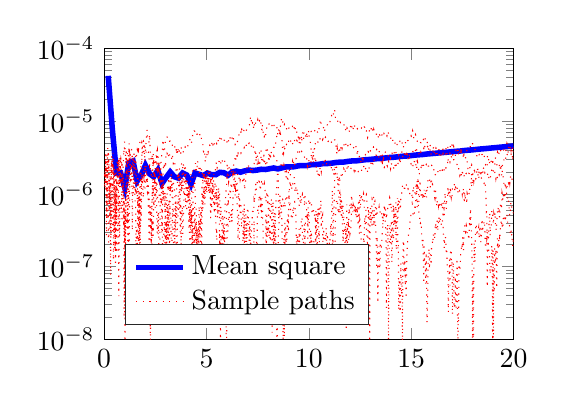
\begin{tikzpicture}

% \begin{axis}[%
% width=5.706cm,
% height=4cm,
% at={(0cm,0cm)},
% scale only axis,
% xmin=0,
% xmax=20,
% ymode=log,
% ymin=1e-10,
% ymax=0.0001,
% yminorticks=true,
% axis background/.style={fill=white},
% title style={font=\bfseries},
% title={error open-loop system},
% legend style={legend cell align=left, align=left, draw=white!15!black}
% ]
\begin{axis}[%
width=5.2cm,
height=3.7cm,
at={(0cm,0cm)},
scale only axis,
xmin=0,
xmax=20,
ymin=1e-08,
ymax=1e-04,
ymode=log,
axis background/.style={fill=white},
legend style={at={(0.05,0.05)}, anchor=south west, legend cell align=left, align=left, draw=white!15!black}
]
\addplot [color=blue, line width=2.0pt]
  table[row sep=crcr]{%
0	0\\
0.202020202020202	4.16999502208996e-05\\
0.404040404040404	7.70351063198471e-06\\
0.606060606060606	1.91559409972505e-06\\
0.808080808080808	1.93658949731201e-06\\
1.01010101010101	1.21237336518482e-06\\
1.21212121212121	2.66970675966661e-06\\
1.41414141414141	2.81922450959295e-06\\
1.61616161616162	1.49799631611757e-06\\
1.81818181818182	1.82560689254214e-06\\
2.02020202020202	2.45696480026046e-06\\
2.22222222222222	1.88479389861182e-06\\
2.42424242424242	1.71695531497272e-06\\
2.62626262626263	2.10890394360482e-06\\
2.82828282828283	1.39197912590424e-06\\
3.03030303030303	1.6747026341524e-06\\
3.23232323232323	1.99751976305593e-06\\
3.43434343434343	1.71733059223393e-06\\
3.63636363636364	1.64227913100189e-06\\
3.83838383838384	1.93327839668588e-06\\
4.04040404040404	1.81247818279963e-06\\
4.24242424242424	1.35595811573062e-06\\
4.44444444444444	1.93179122750832e-06\\
4.64646464646465	1.85387827686734e-06\\
4.84848484848485	1.78172308525527e-06\\
5.05050505050505	1.92560764868801e-06\\
5.25252525252525	1.83051489120253e-06\\
5.45454545454545	1.82939107933157e-06\\
5.65656565656566	1.97339558029152e-06\\
5.85858585858586	1.9483887863834e-06\\
6.06060606060606	1.8041671173223e-06\\
6.26262626262626	2.00222411248892e-06\\
6.46464646464646	2.05321175139142e-06\\
6.66666666666667	1.98321257142836e-06\\
6.86868686868687	2.06734962679268e-06\\
7.07070707070707	2.12287488501052e-06\\
7.27272727272727	2.08870957473154e-06\\
7.47474747474747	2.11993337287861e-06\\
7.67676767676768	2.17555691010297e-06\\
7.87878787878788	2.15923984552761e-06\\
8.08080808080808	2.20872956727098e-06\\
8.28282828282828	2.26510093828327e-06\\
8.48484848484848	2.19973265911587e-06\\
8.68686868686869	2.27202805024729e-06\\
8.88888888888889	2.34179413968359e-06\\
9.09090909090909	2.3357179258239e-06\\
9.29292929292929	2.35690069047644e-06\\
9.49494949494949	2.4277373029049e-06\\
9.6969696969697	2.44000751281706e-06\\
9.8989898989899	2.44118574344842e-06\\
10.1010101010101	2.50719895672632e-06\\
10.3030303030303	2.52626766416747e-06\\
10.5050505050505	2.54893245582739e-06\\
10.7070707070707	2.60023860897743e-06\\
10.9090909090909	2.6071300491429e-06\\
11.1111111111111	2.63423473087317e-06\\
11.3131313131313	2.69084207597384e-06\\
11.5151515151515	2.72257844195214e-06\\
11.7171717171717	2.73306771139126e-06\\
11.9191919191919	2.79079478956689e-06\\
12.1212121212121	2.83047346596641e-06\\
12.3232323232323	2.83950395778837e-06\\
12.5252525252525	2.88578001245677e-06\\
12.7272727272727	2.93262476752684e-06\\
12.9292929292929	2.95847267695918e-06\\
13.1313131313131	2.9935909474557e-06\\
13.3333333333333	3.03992708716807e-06\\
13.5353535353535	3.06401365229264e-06\\
13.7373737373737	3.10809155941226e-06\\
13.9393939393939	3.15513703220452e-06\\
14.1414141414141	3.17823039919982e-06\\
14.3434343434343	3.22327063360824e-06\\
14.5454545454545	3.27429707782018e-06\\
14.7474747474747	3.30225340821527e-06\\
14.9494949494949	3.33515687784264e-06\\
15.1515151515152	3.39381517388831e-06\\
15.3535353535354	3.4322962291202e-06\\
15.5555555555556	3.46203170760557e-06\\
15.7575757575758	3.52064714088643e-06\\
15.959595959596	3.55847721984071e-06\\
16.1616161616162	3.5994281320717e-06\\
16.3636363636364	3.65003702858817e-06\\
16.5656565656566	3.69086707013187e-06\\
16.7676767676768	3.73265120764125e-06\\
16.969696969697	3.78688461302214e-06\\
17.1717171717172	3.83186937739218e-06\\
17.3737373737374	3.8656589462149e-06\\
17.5757575757576	3.92604182827428e-06\\
17.7777777777778	3.97688275239554e-06\\
17.979797979798	4.01335416145516e-06\\
18.1818181818182	4.07132346498969e-06\\
18.3838383838384	4.12481901417198e-06\\
18.5858585858586	4.1712452359484e-06\\
18.7878787878788	4.22319146075711e-06\\
18.989898989899	4.27822340625832e-06\\
19.1919191919192	4.32591263905932e-06\\
19.3939393939394	4.38219397412309e-06\\
19.5959595959596	4.43883502466231e-06\\
19.7979797979798	4.48370008068376e-06\\
20	4.54435179730382e-06\\
};
\addlegendentry{Mean square}

\addplot [color=red, dotted]
  table[row sep=crcr]{%
0	0\\
0.02002002002002	1.98521654822912e-06\\
0.04004004004004	1.99131774052906e-06\\
0.0600600600600601	1.6561511627738e-06\\
0.0800800800800801	2.63521348565232e-06\\
0.1001001001001	1.27894227096942e-06\\
0.12012012012012	4.51230423519763e-07\\
0.14014014014014	2.13816419159851e-06\\
0.16016016016016	1.6836217758506e-06\\
0.18018018018018	2.92109002934421e-06\\
0.2002002002002	2.63064409624687e-06\\
0.22022022022022	3.00054624835369e-06\\
0.24024024024024	1.92803114788257e-06\\
0.26026026026026	1.74389153043655e-06\\
0.28028028028028	8.93994503161616e-07\\
0.3003003003003	3.28462823144721e-07\\
0.32032032032032	4.89481395250572e-07\\
0.34034034034034	5.88774672455164e-07\\
0.36036036036036	1.81883792434207e-06\\
0.38038038038038	2.47714332546284e-06\\
0.4004004004004	2.28750537662506e-06\\
0.42042042042042	1.26288026849111e-06\\
0.44044044044044	1.21308996521315e-06\\
0.46046046046046	1.23952723291602e-06\\
0.48048048048048	1.13274886941821e-06\\
0.500500500500501	2.21006383704863e-06\\
0.520520520520521	1.87661421501879e-06\\
0.540540540540541	1.71403325774459e-07\\
0.560560560560561	1.23294834079988e-06\\
0.580580580580581	1.11957600958159e-06\\
0.600600600600601	1.93266240806432e-07\\
0.620620620620621	3.7166232416048e-07\\
0.640640640640641	8.81341439649679e-07\\
0.660660660660661	2.57162933163082e-06\\
0.680680680680681	2.91380399783062e-06\\
0.700700700700701	2.82429377667973e-06\\
0.720720720720721	1.2689251073423e-06\\
0.740740740740741	1.38310913721983e-06\\
0.760760760760761	2.56400584757182e-06\\
0.780780780780781	2.77087444225802e-06\\
0.800800800800801	1.49134527929837e-06\\
0.820820820820821	1.50444655258226e-06\\
0.840840840840841	1.79113490605532e-06\\
0.860860860860861	1.59784331515816e-06\\
0.880880880880881	1.54050165034478e-06\\
0.900900900900901	1.87845968501091e-06\\
0.920920920920921	1.69705347379621e-06\\
0.940940940940941	7.26563224774688e-07\\
0.960960960960961	3.55787706372817e-07\\
0.980980980980981	8.14743625560327e-07\\
1.001001001001	4.63956475829413e-07\\
1.02102102102102	3.19230415913467e-07\\
1.04104104104104	2.20648642028528e-07\\
1.06106106106106	8.76168745501975e-07\\
1.08108108108108	1.31713909042676e-06\\
1.1011011011011	1.40177932433467e-06\\
1.12112112112112	1.10080318414892e-06\\
1.14114114114114	3.83825239200926e-07\\
1.16116116116116	8.92942094005949e-07\\
1.18118118118118	2.08869698344381e-06\\
1.2012012012012	6.38405270809992e-07\\
1.22122122122122	1.02810065920243e-06\\
1.24124124124124	1.16648188827952e-06\\
1.26126126126126	2.3645913086294e-06\\
1.28128128128128	2.59605699404938e-06\\
1.3013013013013	2.05079510885789e-06\\
1.32132132132132	2.31566786362173e-06\\
1.34134134134134	2.10627747386329e-06\\
1.36136136136136	2.86170179318446e-06\\
1.38138138138138	3.28522438633682e-06\\
1.4014014014014	2.87226552722934e-06\\
1.42142142142142	1.83682988063227e-06\\
1.44144144144144	1.85891940425315e-06\\
1.46146146146146	1.40908679758467e-06\\
1.48148148148148	1.45611551327743e-06\\
1.5015015015015	1.20428019444876e-06\\
1.52152152152152	1.14728921635685e-06\\
1.54154154154154	1.55033569764706e-06\\
1.56156156156156	1.02921661986707e-06\\
1.58158158158158	9.5760624725973e-07\\
1.6016016016016	1.1627020942862e-06\\
1.62162162162162	8.75422895657185e-07\\
1.64164164164164	6.97121671017906e-07\\
1.66166166166166	3.66151976273991e-07\\
1.68168168168168	5.48117491876677e-08\\
1.7017017017017	3.53878972357012e-07\\
1.72172172172172	2.26195735122615e-07\\
1.74174174174174	4.52626505001131e-07\\
1.76176176176176	1.48618177732241e-07\\
1.78178178178178	1.01622386628968e-06\\
1.8018018018018	4.23985456091329e-07\\
1.82182182182182	5.41583411255212e-07\\
1.84184184184184	3.05511805164061e-06\\
1.86186186186186	4.73595218361229e-06\\
1.88188188188188	3.97519758611368e-06\\
1.9019019019019	3.66412340345374e-06\\
1.92192192192192	3.89849750829642e-06\\
1.94194194194194	4.08216510041035e-06\\
1.96196196196196	4.05679964019178e-06\\
1.98198198198198	3.13317086998629e-06\\
2.002002002002	2.03960177928537e-06\\
2.02202202202202	2.16785075338759e-06\\
2.04204204204204	2.52249491925791e-06\\
2.06206206206206	2.13228623438556e-06\\
2.08208208208208	1.57894031472626e-06\\
2.1021021021021	1.0978444720059e-06\\
2.12212212212212	1.04546947142191e-06\\
2.14214214214214	1.18666567557011e-06\\
2.16216216216216	1.28750892913363e-06\\
2.18218218218218	8.94079891202645e-07\\
2.2022022022022	3.8612689595131e-07\\
2.22222222222222	2.96366676375411e-07\\
2.24224224224224	2.57806047493389e-07\\
2.26226226226226	5.76601717248341e-09\\
2.28228228228228	1.08744213283947e-07\\
2.3023023023023	2.09298236286098e-07\\
2.32232232232232	4.02825180970234e-07\\
2.34234234234234	7.61477481685127e-07\\
2.36236236236236	1.18501870939214e-06\\
2.38238238238238	1.44195796281771e-06\\
2.4024024024024	1.16217855882021e-06\\
2.42242242242242	1.25829223617331e-06\\
2.44244244244244	1.32350715353694e-06\\
2.46246246246246	1.75339137574633e-06\\
2.48248248248248	1.27243762319223e-06\\
2.5025025025025	1.74497439090794e-06\\
2.52252252252252	9.29614575614293e-07\\
2.54254254254254	1.02339676338066e-06\\
2.56256256256256	1.52922188637048e-06\\
2.58258258258258	1.50867599288614e-06\\
2.6026026026026	9.63973780336514e-07\\
2.62262262262262	8.14018470571186e-07\\
2.64264264264264	8.03805934681531e-07\\
2.66266266266266	7.50878394848981e-07\\
2.68268268268268	8.19328682699029e-07\\
2.7027027027027	1.18030566717218e-06\\
2.72272272272272	9.42327056653623e-07\\
2.74274274274274	9.81618753763188e-07\\
2.76276276276276	8.85739495860662e-07\\
2.78278278278278	7.24835974845324e-07\\
2.8028028028028	7.58769971493923e-07\\
2.82282282282282	2.81321842248312e-07\\
2.84284284284284	6.40601968897622e-07\\
2.86286286286286	6.13278825382933e-08\\
2.88288288288288	9.80280049566145e-08\\
2.9029029029029	2.30558916615242e-07\\
2.92292292292292	2.91446019476973e-07\\
2.94294294294294	4.1313347697703e-07\\
2.96296296296296	2.73610569130118e-07\\
2.98298298298298	1.84077785069614e-07\\
3.003003003003	1.51919575487685e-07\\
3.02302302302302	9.81365140570323e-07\\
3.04304304304304	6.2943467598664e-07\\
3.06306306306306	6.18913850678258e-07\\
3.08308308308308	1.11122616259629e-06\\
3.1031031031031	1.19500344954575e-06\\
3.12312312312312	1.32622938352889e-06\\
3.14314314314314	1.07910949552287e-06\\
3.16316316316316	1.66031500239481e-06\\
3.18318318318318	1.29465481387343e-06\\
3.2032032032032	1.04104586133805e-06\\
3.22322322322322	1.31568143047237e-06\\
3.24324324324324	1.23330365812593e-06\\
3.26326326326326	1.58695942446157e-06\\
3.28328328328328	1.73918688525821e-06\\
3.3033033033033	1.45247969112736e-06\\
3.32332332332332	8.83895807854491e-07\\
3.34334334334334	1.2920649484403e-06\\
3.36336336336336	1.52125762924768e-06\\
3.38338338338338	1.50072314981924e-06\\
3.4034034034034	1.19069364607757e-06\\
3.42342342342342	1.1589450901214e-06\\
3.44344344344344	1.10763040435655e-06\\
3.46346346346346	8.45131239122477e-07\\
3.48348348348348	7.18276827860688e-07\\
3.5035035035035	4.02009101296639e-07\\
3.52352352352352	2.13688458361014e-07\\
3.54354354354354	1.54277277998995e-08\\
3.56356356356356	1.22785174626277e-07\\
3.58358358358358	3.92042979145687e-07\\
3.6036036036036	4.92182063870184e-07\\
3.62362362362362	5.27719947567079e-07\\
3.64364364364364	6.94074621462263e-07\\
3.66366366366366	7.34931232744364e-07\\
3.68368368368368	6.10496850242619e-07\\
3.7037037037037	7.69823680780044e-07\\
3.72372372372372	9.95413897758697e-07\\
3.74374374374374	1.04385846689752e-06\\
3.76376376376376	1.15269867869221e-06\\
3.78378378378378	1.04616328439811e-06\\
3.8038038038038	1.49387620015406e-06\\
3.82382382382382	1.93633632634711e-06\\
3.84384384384384	2.32201127537986e-06\\
3.86386386386386	1.97353569016452e-06\\
3.88388388388388	1.90282609117224e-06\\
3.9039039039039	1.35617168594631e-06\\
3.92392392392392	1.85169336295397e-06\\
3.94394394394394	2.35568934644055e-06\\
3.96396396396396	2.49244695091477e-06\\
3.98398398398398	2.09027311934505e-06\\
4.004004004004	1.66340518559153e-06\\
4.02402402402402	1.29457345188206e-06\\
4.04404404404404	1.08962020393689e-06\\
4.06406406406406	1.28982539678649e-06\\
4.08408408408408	9.33530944021215e-07\\
4.1041041041041	8.8557047716343e-07\\
4.12412412412412	8.07569793028688e-07\\
4.14414414414414	8.91416838210882e-07\\
4.16416416416416	7.90700024373447e-07\\
4.18418418418418	4.35965430872953e-07\\
4.2042042042042	7.6246568065939e-07\\
4.22422422422422	7.9187675929862e-07\\
4.24424424424424	6.3089213269294e-07\\
4.26426426426426	3.84034063034653e-07\\
4.28428428428428	6.04484265372239e-07\\
4.3043043043043	3.94070337087883e-08\\
4.32432432432432	5.20044848138738e-07\\
4.34434434434434	8.49237208129345e-07\\
4.36436436436436	5.37620584095373e-07\\
4.38438438438438	1.51087341503425e-07\\
4.4044044044044	8.47567113608099e-08\\
4.42442442442442	4.37187383663548e-07\\
4.44444444444444	4.36184839016952e-07\\
4.46446446446446	4.2996643172966e-07\\
4.48448448448448	2.52158529429564e-07\\
4.5045045045045	4.05634894818537e-07\\
4.52452452452452	2.96455050978092e-08\\
4.54454454454454	3.24311228214968e-07\\
4.56456456456456	1.4882709628721e-07\\
4.58458458458458	3.38463756756204e-07\\
4.6046046046046	3.36676415905977e-07\\
4.62462462462462	2.76750877971769e-07\\
4.64464464464464	9.99274485245944e-08\\
4.66466466466466	1.07471371833146e-07\\
4.68468468468468	2.87648874517558e-08\\
4.7047047047047	4.68488968897101e-07\\
4.72472472472472	3.92492853468042e-07\\
4.74474474474474	4.71936195073092e-07\\
4.76476476476476	6.54429378727961e-07\\
4.78478478478478	5.47763422568637e-07\\
4.8048048048048	6.58962127318836e-07\\
4.82482482482482	6.7752502485676e-07\\
4.84484484484484	8.35308604907105e-07\\
4.86486486486486	1.07538014765405e-06\\
4.88488488488488	1.01954798104017e-06\\
4.9049049049049	1.23449859270752e-06\\
4.92492492492492	9.14191022808182e-07\\
4.94494494494494	1.13489025214256e-06\\
4.96496496496496	1.50169024316122e-06\\
4.98498498498498	1.50573545086532e-06\\
5.00500500500501	1.09247284082781e-06\\
5.02502502502503	1.46791852403494e-06\\
5.04504504504505	1.35755326835563e-06\\
5.06506506506507	1.48558277470347e-06\\
5.08508508508509	1.54232627492231e-06\\
5.10510510510511	1.36584233073727e-06\\
5.12512512512513	1.16540489461739e-06\\
5.14514514514515	1.01861986503147e-06\\
5.16516516516517	1.42496669105562e-06\\
5.18518518518519	1.36870603112286e-06\\
5.20520520520521	1.46033666926994e-06\\
5.22522522522523	1.18288670420612e-06\\
5.24524524524525	1.23173389214581e-06\\
5.26526526526527	1.22024169244795e-06\\
5.28528528528529	1.22187829858182e-06\\
5.30530530530531	8.6187061679023e-07\\
5.32532532532533	8.31480112117217e-07\\
5.34534534534535	7.31318333579892e-07\\
5.36536536536537	1.03784505115416e-06\\
5.38538538538539	5.3564258454049e-07\\
5.40540540540541	9.05493976683406e-07\\
5.42542542542543	7.21499596674387e-07\\
5.44544544544545	4.9449664015285e-07\\
5.46546546546547	3.60568681908847e-07\\
5.48548548548549	2.56215066915975e-07\\
5.50550550550551	3.35911595207301e-07\\
5.52552552552553	6.68397544885761e-08\\
5.54554554554555	2.04830237672163e-07\\
5.56556556556557	1.61236634022941e-07\\
5.58558558558559	1.26862951387096e-07\\
5.60560560560561	9.89400957478564e-08\\
5.62562562562563	5.15267444598051e-08\\
5.64564564564565	3.00817059111395e-07\\
5.66566566566567	1.03816649522586e-07\\
5.68568568568569	6.6192232398097e-09\\
5.70570570570571	7.39442991980406e-08\\
5.72572572572573	7.30877041008915e-08\\
5.74574574574575	2.83799687181155e-07\\
5.76576576576577	2.81903579023093e-07\\
5.78578578578579	2.6217094457729e-07\\
5.80580580580581	2.79262922792841e-07\\
5.82582582582583	5.0685185316747e-08\\
5.84584584584585	2.26152633379031e-07\\
5.86586586586587	3.55145129774986e-07\\
5.88588588588589	2.30702139542897e-07\\
5.90590590590591	1.68882539519547e-08\\
5.92592592592593	1.35927082069665e-07\\
5.94594594594595	2.01362267338275e-07\\
5.96596596596597	3.35938604968894e-07\\
5.98598598598599	6.36160822147066e-07\\
6.00600600600601	7.34360673566268e-07\\
6.02602602602603	6.72773648256051e-07\\
6.04604604604605	8.43419256578018e-07\\
6.06606606606607	7.99111701248926e-07\\
6.08608608608609	1.05825883361983e-06\\
6.10610610610611	1.0454794348493e-06\\
6.12612612612613	1.13047696001897e-06\\
6.14614614614615	1.11833979965802e-06\\
6.16616616616617	8.74872682853473e-07\\
6.18618618618619	1.19984741033773e-06\\
6.20620620620621	1.44269489393884e-06\\
6.22622622622623	1.27645805319463e-06\\
6.24624624624625	1.28059729872454e-06\\
6.26626626626627	1.31499613262712e-06\\
6.28628628628629	1.38075467028398e-06\\
6.30630630630631	1.35785908258047e-06\\
6.32632632632633	1.29116972325314e-06\\
6.34634634634635	1.3020895990317e-06\\
6.36636636636637	1.33844072362415e-06\\
6.38638638638639	1.92364288451322e-06\\
6.40640640640641	1.54829065401668e-06\\
6.42642642642643	1.27109516161373e-06\\
6.44644644644645	1.30414451348866e-06\\
6.46646646646647	1.50805925757755e-06\\
6.48648648648649	1.48544358242594e-06\\
6.50650650650651	1.30290906152498e-06\\
6.52652652652653	1.08984480139038e-06\\
6.54654654654655	9.42983878189481e-07\\
6.56656656656657	8.54748391777491e-07\\
6.58658658658659	1.02425480703688e-06\\
6.60660660660661	6.13668552295996e-07\\
6.62662662662663	8.37416871636789e-07\\
6.64664664664665	5.83650064451674e-07\\
6.66666666666667	5.0259201592335e-07\\
6.68668668668669	7.59896603559084e-07\\
6.70670670670671	3.42760389974151e-07\\
6.72672672672673	4.28225978975584e-07\\
6.74674674674675	4.19146053515065e-07\\
6.76676676676677	4.65927866893956e-07\\
6.78678678678679	6.11749077050286e-07\\
6.80680680680681	3.96224276347731e-07\\
6.82682682682683	2.58257970818233e-07\\
6.84684684684685	4.33723608318697e-07\\
6.86686686686687	8.67249403544786e-08\\
6.88688688688689	1.97933742168623e-07\\
6.90690690690691	4.21553511006921e-07\\
6.92692692692693	5.42429926032732e-07\\
6.94694694694695	1.24755459288337e-07\\
6.96696696696697	3.58714513171387e-07\\
6.98698698698699	2.05705586856077e-07\\
7.00700700700701	1.80508800046071e-07\\
7.02702702702703	1.41695229134257e-07\\
7.04704704704705	4.47803338338785e-08\\
7.06706706706707	1.80170974248363e-07\\
7.08708708708709	2.19996566649779e-07\\
7.10710710710711	3.15320515619536e-07\\
7.12712712712713	3.3501378748845e-07\\
7.14714714714715	2.56763326718507e-07\\
7.16716716716717	1.51065740909757e-07\\
7.18718718718719	2.9026368591771e-07\\
7.20720720720721	3.34550371450302e-07\\
7.22722722722723	3.73343589090771e-07\\
7.24724724724725	5.71713478770869e-07\\
7.26726726726727	5.7282041058473e-07\\
7.28728728728729	5.69061252831062e-07\\
7.30730730730731	5.53118207533457e-07\\
7.32732732732733	7.96958065982021e-07\\
7.34734734734735	7.41476334957632e-07\\
7.36736736736737	1.01812593024007e-06\\
7.38738738738739	9.4925010957514e-07\\
7.40740740740741	1.37123074185227e-06\\
7.42742742742743	1.12367880057827e-06\\
7.44744744744745	1.22444354084685e-06\\
7.46746746746747	1.32479938393739e-06\\
7.48748748748749	1.45568621131224e-06\\
7.50750750750751	1.36029942130432e-06\\
7.52752752752753	1.35596711458222e-06\\
7.54754754754755	1.41724557807393e-06\\
7.56756756756757	1.48374350800494e-06\\
7.58758758758759	1.45600857549089e-06\\
7.60760760760761	1.4762069022609e-06\\
7.62762762762763	1.10086370686691e-06\\
7.64764764764765	1.2714807816907e-06\\
7.66766766766767	1.45770333374324e-06\\
7.68768768768769	1.46640705124164e-06\\
7.70770770770771	1.2749874859959e-06\\
7.72772772772773	1.28265393951493e-06\\
7.74774774774775	1.40654450787807e-06\\
7.76776776776777	1.30393033431321e-06\\
7.78778778778779	1.27772868629744e-06\\
7.80780780780781	1.27510926394689e-06\\
7.82782782782783	1.36521993739367e-06\\
7.84784784784785	1.19099150685852e-06\\
7.86786786786787	1.09397243884016e-06\\
7.88788788788789	8.55713332203168e-07\\
7.90790790790791	7.68218723609017e-07\\
7.92792792792793	8.88318276434589e-07\\
7.94794794794795	1.08323312199491e-06\\
7.96796796796797	1.00274316893261e-06\\
7.98798798798799	6.9031136150282e-07\\
8.00800800800801	9.42640552079963e-07\\
8.02802802802803	5.42677316451058e-07\\
8.04804804804805	2.75050399377516e-07\\
8.06806806806807	2.54692652730235e-07\\
8.08808808808809	3.72526790433484e-07\\
8.10810810810811	2.43996172470564e-07\\
8.12812812812813	3.2819839719495e-07\\
8.14814814814815	1.89952566642565e-07\\
8.16816816816817	1.68416042611823e-07\\
8.18818818818819	2.01056847362689e-07\\
8.20820820820821	1.76778224913387e-07\\
8.22822822822823	5.31276364127228e-08\\
8.24824824824825	3.34411955588886e-08\\
8.26826826826827	1.83261667458529e-07\\
8.28828828828829	3.28745280702228e-07\\
8.30830830830831	9.59457229041387e-08\\
8.32832832832833	5.63402403613464e-07\\
8.34834834834835	4.42445084136315e-07\\
8.36836836836837	3.2868867097085e-07\\
8.38838838838839	2.48607791027057e-07\\
8.40840840840841	1.49818296032374e-08\\
8.42842842842843	8.06441709442221e-08\\
8.44844844844845	7.31975406076239e-10\\
8.46846846846847	2.88272673352822e-08\\
8.48848848848849	7.74723562918891e-08\\
8.50850850850851	2.36803335325964e-07\\
8.52852852852853	3.44157828182009e-07\\
8.54854854854855	4.02834097286098e-07\\
8.56856856856857	4.46653489037749e-07\\
8.58858858858859	4.92239001368528e-07\\
8.60860860860861	5.50645517381461e-07\\
8.62862862862863	5.24309939221818e-07\\
8.64864864864865	5.72635682866701e-07\\
8.66866866866867	5.79572655138417e-07\\
8.68868868868869	7.29805623802604e-07\\
8.70870870870871	8.12053374234422e-07\\
8.72872872872873	8.3649449916299e-07\\
8.74874874874875	8.07623565827861e-07\\
8.76876876876877	6.68274766930616e-07\\
8.78878878878879	6.52631777383431e-07\\
8.80880880880881	7.56989735552867e-07\\
8.82882882882883	6.47392840462812e-07\\
8.84884884884885	7.15619689555412e-07\\
8.86886886886887	8.7082040800425e-07\\
8.88888888888889	9.22605436799006e-07\\
8.90890890890891	9.56848393394234e-07\\
8.92892892892893	7.97377163982207e-07\\
8.94894894894895	8.04765290668858e-07\\
8.96896896896897	8.47546004173241e-07\\
8.98898898898899	8.55233698715464e-07\\
9.00900900900901	9.73571442320414e-07\\
9.02902902902903	1.08100282708594e-06\\
9.04904904904905	8.75284360162089e-07\\
9.06906906906907	6.56750611218473e-07\\
9.08908908908909	7.50471502723192e-07\\
9.10910910910911	5.8236770182691e-07\\
9.12912912912913	5.68849393355345e-07\\
9.14914914914915	4.62772820950178e-07\\
9.16916916916917	5.06461314069138e-07\\
9.18918918918919	4.84605001536181e-07\\
9.20920920920921	4.8754157656063e-07\\
9.22922922922923	6.36746001558663e-07\\
9.24924924924925	5.33802869594051e-07\\
9.26926926926927	7.02513112030123e-07\\
9.28928928928929	7.65702298855075e-07\\
9.30930930930931	7.75626992773469e-07\\
9.32932932932933	6.68082310698122e-07\\
9.34934934934935	5.46943894835479e-07\\
9.36936936936937	5.04012595131115e-07\\
9.38938938938939	2.53700623764552e-07\\
9.40940940940941	1.72085665233527e-07\\
9.42942942942943	2.69475064316255e-07\\
9.44944944944945	2.18940790945266e-07\\
9.46946946946947	2.64414598888523e-07\\
9.48948948948949	1.40831121732836e-07\\
9.50950950950951	8.70682309491323e-08\\
9.52952952952953	3.3412626053853e-07\\
9.54954954954955	2.16918910689564e-07\\
9.56956956956957	2.56770526554147e-07\\
9.58958958958959	2.82137116964902e-07\\
9.60960960960961	3.58910843732113e-07\\
9.62962962962963	4.09083547362273e-07\\
9.64964964964965	4.76077901834143e-07\\
9.66966966966967	4.70996897285397e-07\\
9.68968968968969	2.62286088401962e-07\\
9.70970970970971	1.88932684136749e-07\\
9.72972972972973	1.84084807959576e-07\\
9.74974974974975	2.8921133373911e-07\\
9.76976976976977	3.45190035300421e-07\\
9.78978978978979	3.87745147574492e-07\\
9.80980980980981	1.65780484979174e-07\\
9.82982982982983	3.82446722257204e-07\\
9.84984984984985	4.86962531651836e-07\\
9.86986986986987	5.39569358200729e-07\\
9.88988988988989	4.91626253385519e-07\\
9.90990990990991	4.53944577024505e-07\\
9.92992992992993	4.98024455625591e-07\\
9.94994994994995	3.62899133082315e-07\\
9.96996996996997	6.8261186959828e-07\\
9.98998998998999	7.70388671923907e-07\\
10.01001001001	8.51226437542124e-07\\
10.03003003003	7.41466940108425e-07\\
10.0500500500501	6.73505417867191e-07\\
10.0700700700701	7.94246170432569e-07\\
10.0900900900901	7.87865937999393e-07\\
10.1101101101101	7.97943247458377e-07\\
10.1301301301301	7.17676207343951e-07\\
10.1501501501502	5.6445586539488e-07\\
10.1701701701702	5.36759225660052e-07\\
10.1901901901902	5.99145845050336e-07\\
10.2102102102102	5.26358677761843e-07\\
10.2302302302302	5.95130474320342e-07\\
10.2502502502503	5.10928742912217e-07\\
10.2702702702703	5.00069771723315e-07\\
10.2902902902903	5.21580992844145e-07\\
10.3103103103103	4.47127705950914e-07\\
10.3303303303303	4.90729130022581e-07\\
10.3503503503504	6.01700239850882e-07\\
10.3703703703704	4.90683300680648e-07\\
10.3903903903904	3.80987461885194e-07\\
10.4104104104104	4.7431047425031e-07\\
10.4304304304304	5.43709732828039e-07\\
10.4504504504505	3.83250641701732e-07\\
10.4704704704705	4.15319429978395e-07\\
10.4904904904905	2.37390821295006e-07\\
10.5105105105105	3.18058050398608e-07\\
10.5305305305305	3.98321153748086e-08\\
10.5505505505506	1.3107537885076e-07\\
10.5705705705706	1.11834857746026e-07\\
10.5905905905906	1.05671624129281e-07\\
10.6106106106106	1.21523130117763e-07\\
10.6306306306306	1.95603082675248e-08\\
10.6506506506507	9.46988174407371e-08\\
10.6706706706707	1.1370141155017e-07\\
10.6906906906907	1.16626491157995e-07\\
10.7107107107107	1.16657141511572e-07\\
10.7307307307307	1.90698481662783e-08\\
10.7507507507508	1.15148066087389e-07\\
10.7707707707708	1.88340071731578e-07\\
10.7907907907908	7.38680964320136e-08\\
10.8108108108108	1.69983859338648e-07\\
10.8308308308308	1.43069042361724e-07\\
10.8508508508509	8.93540904758273e-08\\
10.8708708708709	7.10996704712328e-08\\
10.8908908908909	9.68187747431804e-08\\
10.9109109109109	7.16035587393909e-08\\
10.9309309309309	1.40397921162426e-07\\
10.950950950951	1.0207189786292e-07\\
10.970970970971	1.39656392449924e-07\\
10.990990990991	1.67649127278115e-07\\
11.011011011011	2.26821161509436e-07\\
11.031031031031	2.16034937403597e-07\\
11.0510510510511	2.81302365427713e-07\\
11.0710710710711	3.8425934903262e-07\\
11.0910910910911	2.59675967700972e-07\\
11.1111111111111	4.47360708596967e-07\\
11.1311311311311	7.66985455668736e-07\\
11.1511511511512	1.12294204162318e-06\\
11.1711711711712	6.20881577132689e-07\\
11.1911911911912	1.29459033865706e-07\\
11.2112112112112	2.44275894852154e-08\\
11.2312312312312	9.78806816687079e-08\\
11.2512512512513	1.1553341106454e-07\\
11.2712712712713	8.42039924617745e-08\\
11.2912912912913	3.76265705142451e-07\\
11.3113113113113	5.75143579038869e-07\\
11.3313313313313	6.53202734833294e-07\\
11.3513513513514	7.83690946450335e-07\\
11.3713713713714	7.88613148881301e-07\\
11.3913913913914	8.43685106810027e-07\\
11.4114114114114	6.89440425839217e-07\\
11.4314314314314	5.72981692032865e-07\\
11.4514514514515	5.27534705034998e-07\\
11.4714714714715	6.52771322496084e-07\\
11.4914914914915	5.74647406906389e-07\\
11.5115115115115	6.17038592783045e-07\\
11.5315315315315	5.49032740193137e-07\\
11.5515515515516	6.58522913244862e-07\\
11.5715715715716	7.65597878174409e-07\\
11.5915915915916	8.81089881455602e-07\\
11.6116116116116	5.88117847344284e-07\\
11.6316316316316	7.42555882975892e-07\\
11.6516516516517	6.09377176212125e-07\\
11.6716716716717	6.81421755774403e-07\\
11.6916916916917	4.14553032118431e-07\\
11.7117117117117	4.80480011315139e-07\\
11.7317317317317	4.13196382599566e-07\\
11.7517517517518	2.94733036833235e-07\\
11.7717717717718	2.89182768892898e-07\\
11.7917917917918	3.73879556941398e-07\\
11.8118118118118	2.58750883820286e-07\\
11.8318318318318	2.46584217723673e-07\\
11.8518518518519	2.2074956059894e-07\\
11.8718718718719	2.95385881479607e-07\\
11.8918918918919	3.54298732984675e-07\\
11.9119119119119	3.40041967968562e-07\\
11.9319319319319	3.69177448123076e-07\\
11.951951951952	3.00046955050887e-07\\
11.971971971972	3.06659824504672e-07\\
11.991991991992	3.59920336874197e-07\\
12.012012012012	2.83552546656127e-07\\
12.032032032032	3.02931839137348e-07\\
12.0520520520521	3.17714138221221e-07\\
12.0720720720721	4.69168030043321e-07\\
12.0920920920921	5.93472420395659e-07\\
12.1121121121121	6.55702089677362e-07\\
12.1321321321321	6.61490519560711e-07\\
12.1521521521522	6.19313957402369e-07\\
12.1721721721722	7.1128472840582e-07\\
12.1921921921922	6.59401318651277e-07\\
12.2122122122122	6.48916891278005e-07\\
12.2322322322322	5.26553439204757e-07\\
12.2522522522523	5.48096776555636e-07\\
12.2722722722723	5.70400699921873e-07\\
12.2922922922923	4.89015400520615e-07\\
12.3123123123123	5.53647161490076e-07\\
12.3323323323323	4.78512340271573e-07\\
12.3523523523524	6.40965252878253e-07\\
12.3723723723724	5.41651674404319e-07\\
12.3923923923924	6.81465881925297e-07\\
12.4124124124124	6.63999241059395e-07\\
12.4324324324324	8.37414080415146e-07\\
12.4524524524525	7.7420859998007e-07\\
12.4724724724725	7.67924511317295e-07\\
12.4924924924925	9.7279386891142e-07\\
12.5125125125125	6.18925254879208e-07\\
12.5325325325325	7.18558124819609e-07\\
12.5525525525526	9.4344991688848e-07\\
12.5725725725726	9.99101562621088e-07\\
12.5925925925926	7.86114944440645e-07\\
12.6126126126126	8.09597468401531e-07\\
12.6326326326326	8.53129974741576e-07\\
12.6526526526527	9.55979975829158e-07\\
12.6726726726727	1.00344241961376e-06\\
12.6926926926927	8.34944377733103e-07\\
12.7127127127127	6.49249167769798e-07\\
12.7327327327327	8.64051951923663e-07\\
12.7527527527528	8.61010730963075e-07\\
12.7727727727728	8.80426012438114e-07\\
12.7927927927928	9.44488277188265e-07\\
12.8128128128128	9.7081911113072e-07\\
12.8328328328328	8.16716851452445e-07\\
12.8528528528529	7.47928146177404e-07\\
12.8728728728729	7.16397184468277e-07\\
12.8928928928929	5.53301883265289e-07\\
12.9129129129129	5.26481635257428e-07\\
12.9329329329329	4.71208598080767e-07\\
12.952952952953	4.94135670554496e-07\\
12.972972972973	5.00323773842928e-07\\
12.992992992993	4.70179198010751e-07\\
13.013013013013	4.61959039736953e-07\\
13.033033033033	4.74187095192088e-07\\
13.0530530530531	4.29328781672599e-07\\
13.0730730730731	5.58795464880995e-07\\
13.0930930930931	3.40896095039565e-07\\
13.1131131131131	5.94632504422355e-07\\
13.1331331331331	6.00518944269567e-07\\
13.1531531531532	5.69770216412777e-07\\
13.1731731731732	3.58567110715178e-07\\
13.1931931931932	6.04928117225374e-07\\
13.2132132132132	4.60330252719436e-07\\
13.2332332332332	3.60818097567221e-07\\
13.2532532532533	3.79818489529752e-07\\
13.2732732732733	3.43909837511442e-07\\
13.2932932932933	2.23205863773781e-07\\
13.3133133133133	9.42189955205093e-08\\
13.3333333333333	2.61482442491297e-07\\
13.3533533533534	1.79049330975085e-07\\
13.3733733733734	3.16424239004505e-08\\
13.3933933933934	1.1381846249472e-07\\
13.4134134134134	1.68506003108218e-07\\
13.4334334334334	1.89681521281694e-07\\
13.4534534534535	9.95428697312255e-08\\
13.4734734734735	9.23196441759718e-08\\
13.4934934934935	1.95496992234762e-07\\
13.5135135135135	1.92969877095722e-07\\
13.5335335335335	1.71657627708983e-07\\
13.5535535535536	1.98005043701223e-07\\
13.5735735735736	2.41880118943095e-07\\
13.5935935935936	3.0338736254302e-07\\
13.6136136136136	3.63642347372794e-07\\
13.6336336336336	4.1865899446559e-07\\
13.6536536536537	4.76826166397217e-07\\
13.6736736736737	4.66583903276244e-07\\
13.6936936936937	5.08486367509698e-07\\
13.7137137137137	6.76674257689526e-07\\
13.7337337337337	6.72553753486176e-07\\
13.7537537537538	6.012974010043e-07\\
13.7737737737738	5.34392094571095e-07\\
13.7937937937938	4.49554587067548e-07\\
13.8138138138138	5.30938159455122e-07\\
13.8338338338338	5.71528689285884e-07\\
13.8538538538539	6.25133197474083e-07\\
13.8738738738739	6.9152409576054e-07\\
13.8938938938939	7.00683468344404e-07\\
13.9139139139139	6.73599227995043e-07\\
13.9339339339339	7.37445126770938e-07\\
13.953953953954	8.79435332408936e-07\\
13.973973973974	8.42383022659625e-07\\
13.993993993994	7.97463939358024e-07\\
14.014014014014	6.14873294855547e-07\\
14.034034034034	6.80664903496486e-07\\
14.0540540540541	6.54948103519713e-07\\
14.0740740740741	5.73156300980019e-07\\
14.0940940940941	5.64811273413791e-07\\
14.1141141141141	6.27733130306408e-07\\
14.1341341341341	7.12096763139888e-07\\
14.1541541541542	5.70595734802819e-07\\
14.1741741741742	4.10702334342608e-07\\
14.1941941941942	4.62935403115731e-07\\
14.2142142142142	4.42490968166139e-07\\
14.2342342342342	2.72440156819881e-07\\
14.2542542542543	4.32125742840806e-07\\
14.2742742742743	1.68403974382292e-07\\
14.2942942942943	2.1325150779519e-07\\
14.3143143143143	3.07925710390464e-07\\
14.3343343343343	4.18118491950863e-07\\
14.3543543543544	1.74177482387438e-07\\
14.3743743743744	2.00471655811995e-07\\
14.3943943943944	2.53650186420059e-08\\
14.4144144144144	6.80788213448907e-08\\
14.4344344344344	4.94795998250062e-08\\
14.4544544544545	2.5400863550533e-08\\
14.4744744744745	2.3640410882526e-08\\
14.4944944944945	1.11897207278904e-07\\
14.5145145145145	5.33378497412285e-08\\
14.5345345345345	4.08157965641653e-08\\
14.5545545545546	6.66383953804179e-08\\
14.5745745745746	5.64289588384055e-09\\
14.5945945945946	1.00968431113836e-07\\
14.6146146146146	2.13053114385064e-07\\
14.6346346346346	2.29880042483388e-07\\
14.6546546546547	8.2536951697901e-08\\
14.6746746746747	8.09517229368836e-08\\
14.6946946946947	1.27209382885512e-07\\
14.7147147147147	5.42402671838314e-08\\
14.7347347347347	1.01767238258512e-07\\
14.7547547547548	3.67280572523681e-08\\
14.7747747747748	9.01948331297846e-08\\
14.7947947947948	1.46283904473289e-07\\
14.8148148148148	1.91426471313546e-07\\
14.8348348348348	2.39617697576545e-07\\
14.8548548548549	2.6270746479346e-07\\
14.8748748748749	2.74712463092731e-07\\
14.8948948948949	2.99057881934197e-07\\
14.9149149149149	3.0679791008709e-07\\
14.9349349349349	3.75576914957978e-07\\
14.954954954955	4.39336885820333e-07\\
14.974974974975	4.70732425149843e-07\\
14.994994994995	5.34930701063962e-07\\
15.015015015015	5.43260682730706e-07\\
15.035035035035	5.28648739690128e-07\\
15.0550550550551	5.24642253006098e-07\\
15.0750750750751	5.06197726583681e-07\\
15.0950950950951	5.3562532160917e-07\\
15.1151151151151	5.45162558509885e-07\\
15.1351351351351	4.999853200444e-07\\
15.1551551551552	5.22695009992105e-07\\
15.1751751751752	6.66805969732907e-07\\
15.1951951951952	5.91927731626031e-07\\
15.2152152152152	7.73817122619831e-07\\
15.2352352352352	1.11432487170169e-06\\
15.2552552552553	1.09254828916739e-06\\
15.2752752752753	8.297630499644e-07\\
15.2952952952953	6.50234536324969e-07\\
15.3153153153153	8.15758918356626e-07\\
15.3353353353353	7.86421707844172e-07\\
15.3553553553554	6.76288574250084e-07\\
15.3753753753754	5.51535527657663e-07\\
15.3953953953954	5.04780513236644e-07\\
15.4154154154154	5.01980006479007e-07\\
15.4354354354354	3.83147401453924e-07\\
15.4554554554555	3.92726366629289e-07\\
15.4754754754755	3.65371710110814e-07\\
15.4954954954955	3.81052779800279e-07\\
15.5155155155155	2.63354920041271e-07\\
15.5355355355355	2.3779507362243e-07\\
15.5555555555556	1.91891133403929e-07\\
15.5755755755756	2.36548323995323e-07\\
15.5955955955956	1.28047497483103e-07\\
15.6156156156156	5.85521057254827e-08\\
15.6356356356356	1.90157304406915e-07\\
15.6556556556557	1.09419426334792e-07\\
15.6756756756757	1.05693556589321e-07\\
15.6956956956957	1.0800805547954e-07\\
15.7157157157157	5.85792601226551e-08\\
15.7357357357357	1.56153502637151e-07\\
15.7557557557558	5.47781131290003e-08\\
15.7757757757758	1.71590308561159e-08\\
15.7957957957958	2.66180649047355e-08\\
15.8158158158158	6.19706462819524e-08\\
15.8358358358358	1.40689225772868e-07\\
15.8558558558559	1.48684013412442e-07\\
15.8758758758759	1.78029031482566e-07\\
15.8958958958959	9.27586604241153e-08\\
15.9159159159159	1.3236633913008e-07\\
15.9359359359359	1.52816420198743e-07\\
15.955955955956	1.24838025334589e-07\\
15.975975975976	1.05269500774968e-07\\
15.995995995996	1.84961260807608e-07\\
16.016016016016	2.00592824330719e-07\\
16.036036036036	2.07136080416025e-07\\
16.0560560560561	2.51298138680718e-07\\
16.0760760760761	2.2819265306573e-07\\
16.0960960960961	2.88310992664574e-07\\
16.1161161161161	2.89114115524794e-07\\
16.1361361361361	2.682945642182e-07\\
16.1561561561562	2.40942261142869e-07\\
16.1761761761762	3.41103780986327e-07\\
16.1961961961962	4.01325751645645e-07\\
16.2162162162162	3.2193286470125e-07\\
16.2362362362362	3.70708939615579e-07\\
16.2562562562563	4.09224117265811e-07\\
16.2762762762763	4.28453581004868e-07\\
16.2962962962963	3.06528779650868e-07\\
16.3163163163163	3.65030688312745e-07\\
16.3363363363363	4.21219864149561e-07\\
16.3563563563564	4.79435025882581e-07\\
16.3763763763764	3.97305626014197e-07\\
16.3963963963964	4.65222051525178e-07\\
16.4164164164164	4.80308211913547e-07\\
16.4364364364364	4.02641660401705e-07\\
16.4564564564565	3.72328772464736e-07\\
16.4764764764765	3.87739742866803e-07\\
16.4964964964965	4.29248939741646e-07\\
16.5165165165165	4.46845727816317e-07\\
16.5365365365365	4.15061677555275e-07\\
16.5565565565566	4.00974900019933e-07\\
16.5765765765766	2.80370042849034e-07\\
16.5965965965966	2.55046877098108e-07\\
16.6166166166166	1.79800936918751e-07\\
16.6366366366366	2.25184320898606e-07\\
16.6566566566567	2.36007167222594e-07\\
16.6766766766767	2.58141663006743e-07\\
16.6966966966967	2.1051097458584e-07\\
16.7167167167167	1.53340528859251e-07\\
16.7367367367367	1.68388491226591e-07\\
16.7567567567568	1.13943787444141e-07\\
16.7767767767768	9.47127427448816e-08\\
16.7967967967968	8.37791109279946e-08\\
16.8168168168168	2.36021069643678e-08\\
16.8368368368368	6.85040189805191e-08\\
16.8568568568569	7.73265396880125e-08\\
16.8768768768769	1.2506926114829e-07\\
16.8968968968969	5.51750252373774e-08\\
16.9169169169169	1.49245399036678e-07\\
16.9369369369369	1.73619816616806e-07\\
16.956956956957	1.57615494072424e-07\\
16.976976976977	1.03428577303647e-07\\
16.996996996997	1.2094843036198e-07\\
17.017017017017	2.20347555072142e-08\\
17.037037037037	5.21949377023881e-08\\
17.0570570570571	1.1565888365653e-07\\
17.0770770770771	7.72782735785226e-08\\
17.0970970970971	2.76361114489109e-08\\
17.1171171171171	2.97607813163038e-08\\
17.1371371371371	2.61018225809013e-08\\
17.1571571571572	7.32230390048602e-08\\
17.1771771771772	4.0402813510791e-08\\
17.1971971971972	2.74720716411329e-08\\
17.2172172172172	4.80128754374849e-08\\
17.2372372372372	1.30053750805211e-07\\
17.2572572572573	7.96562580595047e-08\\
17.2772772772773	3.86513721881218e-09\\
17.2972972972973	2.18888851187952e-08\\
17.3173173173173	1.70183322507007e-08\\
17.3373373373373	1.09310615613101e-07\\
17.3573573573574	8.84688699298475e-08\\
17.3773773773774	8.82599524234872e-08\\
17.3973973973974	1.00282725950939e-07\\
17.4174174174174	1.49535506039123e-07\\
17.4374374374374	1.71061543699039e-07\\
17.4574574574575	1.81029970969202e-07\\
17.4774774774775	2.05219425066352e-07\\
17.4974974974975	1.7614267486248e-07\\
17.5175175175175	2.49102259097716e-07\\
17.5375375375375	2.53462973618835e-07\\
17.5575575575576	1.66841701487071e-07\\
17.5775775775776	2.86541798064583e-07\\
17.5975975975976	3.54291625732122e-07\\
17.6176176176176	3.68717104582186e-07\\
17.6376376376376	3.30282716385547e-07\\
17.6576576576577	2.98645576750258e-07\\
17.6776776776777	3.07850131631425e-07\\
17.6976976976977	3.67187484828064e-07\\
17.7177177177177	3.49229052363341e-07\\
17.7377377377377	2.90350986336143e-07\\
17.7577577577578	2.60836913703714e-07\\
17.7777777777778	2.71386884673263e-07\\
17.7977977977978	2.62676513921296e-07\\
17.8178178178178	2.3166396122688e-07\\
17.8378378378378	3.21205198394785e-07\\
17.8578578578579	4.7148216765639e-07\\
17.8778778778779	3.69833066864875e-07\\
17.8978978978979	6.29665106479389e-07\\
17.9179179179179	4.49717633340128e-07\\
17.9379379379379	3.65337583922001e-07\\
17.957957957958	2.24163483427138e-07\\
17.977977977978	1.16363197375911e-07\\
17.997997997998	9.06770158544267e-09\\
18.018018018018	7.50170560121701e-08\\
18.038038038038	2.35572641123974e-09\\
18.0580580580581	7.2329220230546e-08\\
18.0780780780781	2.12689032357445e-07\\
18.0980980980981	1.19768763473905e-07\\
18.1181181181181	1.14340868989501e-07\\
18.1381381381381	2.75926397745069e-07\\
18.1581581581582	3.74090676147471e-07\\
18.1781781781782	3.88779891727968e-07\\
18.1981981981982	2.9388418405174e-07\\
18.2182182182182	2.7114487311815e-07\\
18.2382382382382	3.05962654557768e-07\\
18.2582582582583	2.89389987491303e-07\\
18.2782782782783	3.23879192723582e-07\\
18.2982982982983	3.45321583110854e-07\\
18.3183183183183	2.43576300624757e-07\\
18.3383383383383	2.89724844631205e-07\\
18.3583583583584	3.63010259581886e-07\\
18.3783783783784	3.19155808040433e-07\\
18.3983983983984	2.17471882419333e-07\\
18.4184184184184	2.41732951169437e-07\\
18.4384384384384	3.23995852374421e-07\\
18.4584584584585	4.5314141546026e-07\\
18.4784784784785	4.11119308733289e-07\\
18.4984984984985	3.31663032988503e-07\\
18.5185185185185	3.35033916550986e-07\\
18.5385385385385	3.36858319974368e-07\\
18.5585585585586	4.12343872708057e-07\\
18.5785785785786	4.27554411208792e-07\\
18.5985985985986	3.14777668760103e-07\\
18.6186186186186	2.03815689672076e-07\\
18.6386386386386	1.78407491713855e-07\\
18.6586586586587	2.59965679985231e-07\\
18.6786786786787	3.00665543527324e-07\\
18.6986986986987	2.39653184451284e-07\\
18.7187187187187	2.54113715078458e-07\\
18.7387387387387	3.02992351545153e-07\\
18.7587587587588	2.23272235119464e-07\\
18.7787787787788	1.81895082224967e-07\\
18.7987987987988	1.55642917113247e-07\\
18.8188188188188	1.50708434095175e-07\\
18.8388388388388	1.13316350209189e-07\\
18.8588588588589	7.82992386854972e-08\\
18.8788788788789	9.91675096821781e-08\\
18.8988988988989	9.75634910329622e-08\\
18.9189189189189	1.15554989852474e-07\\
18.9389389389389	1.97495824367824e-07\\
18.958958958959	1.2880592281311e-07\\
18.978978978979	8.76124605217306e-09\\
18.998998998999	1.72892994941546e-07\\
19.019019019019	1.02661366742138e-08\\
19.039039039039	9.14578605043173e-08\\
19.0590590590591	4.49996281879097e-08\\
19.0790790790791	1.78345410798318e-07\\
19.0990990990991	1.19876518308817e-07\\
19.1191191191191	1.0974728372196e-07\\
19.1391391391391	1.74957345436633e-07\\
19.1591591591592	1.18495232025546e-07\\
19.1791791791792	5.04476448387015e-08\\
19.1991991991992	1.29991426492607e-07\\
19.2192192192192	2.45780625515082e-07\\
19.2392392392392	1.74788536846599e-07\\
19.2592592592593	1.9462242592573e-07\\
19.2792792792793	2.31985388171805e-07\\
19.2992992992993	1.74479144460828e-07\\
19.3193193193193	2.42745484172923e-07\\
19.3393393393393	2.30239537401195e-07\\
19.3593593593594	3.50083870421093e-07\\
19.3793793793794	3.77187525318188e-07\\
19.3993993993994	4.22806397657468e-07\\
19.4194194194194	3.72523665860047e-07\\
19.4394394394394	4.17238954490987e-07\\
19.4594594594595	3.31534819462763e-07\\
19.4794794794795	3.3392152364237e-07\\
19.4994994994995	4.61730517819294e-07\\
19.5195195195195	4.19122845402164e-07\\
19.5395395395395	4.58128527333873e-07\\
19.5595595595596	4.92155802753709e-07\\
19.5795795795796	5.08516851003965e-07\\
19.5995995995996	4.59798802962746e-07\\
19.6196196196196	4.6610381142948e-07\\
19.6396396396396	5.05238857741428e-07\\
19.6596596596597	5.3571007033582e-07\\
19.6796796796797	5.25872685610135e-07\\
19.6996996996997	4.62380475193027e-07\\
19.7197197197197	3.86050040062871e-07\\
19.7397397397397	3.80785268727344e-07\\
19.7597597597598	3.96231392846035e-07\\
19.7797797797798	3.82828785179757e-07\\
19.7997997997998	3.778838121532e-07\\
19.8198198198198	3.3124083591225e-07\\
19.8398398398398	2.88327945727088e-07\\
19.8598598598599	2.77500046218992e-07\\
19.8798798798799	3.13368167415802e-07\\
19.8998998998999	2.60984549318438e-07\\
19.9199199199199	2.82652109702309e-07\\
19.9399399399399	2.15812108594784e-07\\
19.95995995996	1.93449545162613e-07\\
19.97997997998	2.32489529530007e-07\\
20	2.11416240179304e-07\\
};
\addlegendentry{Sample paths}

\addplot [color=red, dotted]
  table[row sep=crcr]{%
0	0\\
0.02002002002002	1.87085760713168e-06\\
0.04004004004004	1.62429791758058e-06\\
0.0600600600600601	1.79948730710559e-06\\
0.0800800800800801	2.43339335074466e-06\\
0.1001001001001	1.23985743863839e-06\\
0.12012012012012	5.10839964550424e-07\\
0.14014014014014	9.81945758498193e-07\\
0.16016016016016	1.14851441073681e-06\\
0.18018018018018	1.82793437617227e-06\\
0.2002002002002	3.08685613899112e-06\\
0.22022022022022	2.14206750281179e-06\\
0.24024024024024	2.54908741434464e-06\\
0.26026026026026	7.1935721313715e-07\\
0.28028028028028	1.25267149170524e-06\\
0.3003003003003	1.63795800598012e-06\\
0.32032032032032	1.36301271031204e-06\\
0.34034034034034	1.47791899042601e-06\\
0.36036036036036	2.77916589324153e-06\\
0.38038038038038	3.32104624231631e-06\\
0.4004004004004	3.05971407371576e-06\\
0.42042042042042	2.96581275701663e-06\\
0.44044044044044	2.4100103858634e-06\\
0.46046046046046	2.25195908466604e-06\\
0.48048048048048	1.12983029335801e-06\\
0.500500500500501	1.38147664211049e-06\\
0.520520520520521	8.34651359141843e-07\\
0.540540540540541	9.58080243269471e-07\\
0.560560560560561	6.37770473077704e-07\\
0.580580580580581	4.39784646886592e-07\\
0.600600600600601	7.78277541482142e-07\\
0.620620620620621	1.52353741203815e-07\\
0.640640640640641	2.70095484806971e-07\\
0.660660660660661	3.77859848334522e-07\\
0.680680680680681	3.31744312620694e-07\\
0.700700700700701	1.45822690511717e-06\\
0.720720720720721	1.54978072242031e-06\\
0.740740740740741	1.41060270873646e-06\\
0.760760760760761	1.23650947927079e-06\\
0.780780780780781	2.04760386190321e-06\\
0.800800800800801	2.85020225310864e-06\\
0.820820820820821	1.23524968031514e-06\\
0.840840840840841	1.82520455581439e-06\\
0.860860860860861	1.69955893940381e-06\\
0.880880880880881	1.95397796689437e-06\\
0.900900900900901	1.11809951958032e-06\\
0.920920920920921	1.75222244821688e-06\\
0.940940940940941	1.7663024322192e-06\\
0.960960960960961	1.0028494763399e-06\\
0.980980980980981	2.72725498768058e-07\\
1.001001001001	3.48570516620611e-07\\
1.02102102102102	2.55865947723404e-07\\
1.04104104104104	7.43305079032308e-08\\
1.06106106106106	6.21906897478391e-07\\
1.08108108108108	7.9205417472734e-07\\
1.1011011011011	1.12648958578e-06\\
1.12112112112112	2.02464630246802e-06\\
1.14114114114114	2.62249114932988e-06\\
1.16116116116116	2.48356799262622e-06\\
1.18118118118118	2.8401251045735e-06\\
1.2012012012012	3.10091527307214e-06\\
1.22122122122122	2.86818300395335e-06\\
1.24124124124124	3.69907181643112e-06\\
1.26126126126126	2.45938593274938e-06\\
1.28128128128128	3.3061935321814e-06\\
1.3013013013013	3.16104197799485e-06\\
1.32132132132132	3.3295035475984e-06\\
1.34134134134134	3.28913849583591e-06\\
1.36136136136136	3.27433526760146e-06\\
1.38138138138138	3.17398323178866e-06\\
1.4014014014014	2.83287236792355e-06\\
1.42142142142142	2.87247458495526e-06\\
1.44144144144144	2.97990073008932e-06\\
1.46146146146146	3.61215884402953e-06\\
1.48148148148148	2.61869150281842e-06\\
1.5015015015015	2.38458624292577e-06\\
1.52152152152152	2.153491296481e-06\\
1.54154154154154	1.80774851283882e-06\\
1.56156156156156	2.27263260636203e-06\\
1.58158158158158	2.28204059251619e-06\\
1.6016016016016	2.19835386876625e-06\\
1.62162162162162	2.16475587048111e-06\\
1.64164164164164	1.05589960338026e-06\\
1.66166166166166	1.62322000814707e-06\\
1.68168168168168	1.437875517662e-06\\
1.7017017017017	3.32706618028166e-07\\
1.72172172172172	1.07327867979644e-06\\
1.74174174174174	6.68004739091696e-07\\
1.76176176176176	3.36068829697848e-07\\
1.78178178178178	1.41098333333662e-06\\
1.8018018018018	2.76050085059676e-06\\
1.82182182182182	2.51746449128476e-06\\
1.84184184184184	2.71333427700458e-06\\
1.86186186186186	3.71255395061989e-06\\
1.88188188188188	3.98891082100494e-06\\
1.9019019019019	4.17965623221771e-06\\
1.92192192192192	4.61142271902934e-06\\
1.94194194194194	4.03419578790806e-06\\
1.96196196196196	3.24039893662871e-06\\
1.98198198198198	3.16775081792738e-06\\
2.002002002002	3.36060666620679e-06\\
2.02202202202202	3.93919656845834e-06\\
2.04204204204204	4.80341146570282e-06\\
2.06206206206206	5.13309462491976e-06\\
2.08208208208208	6.59082495607154e-06\\
2.1021021021021	7.5667693966745e-06\\
2.12212212212212	5.73575714719536e-06\\
2.14214214214214	5.75041952685472e-06\\
2.16216216216216	5.41344701585859e-06\\
2.18218218218218	5.26732277783837e-06\\
2.2022022022022	5.05032482902738e-06\\
2.22222222222222	6.53038085591991e-06\\
2.24224224224224	4.83429136000195e-06\\
2.26226226226226	3.52065973326519e-06\\
2.28228228228228	3.39421552660113e-06\\
2.3023023023023	2.74436868795397e-06\\
2.32232232232232	2.87180899902861e-06\\
2.34234234234234	3.50993951765107e-06\\
2.36236236236236	2.92715447270789e-06\\
2.38238238238238	2.29743823752843e-06\\
2.4024024024024	3.59253959054989e-06\\
2.42242242242242	2.81932530285809e-06\\
2.44244244244244	3.06147158646755e-06\\
2.46246246246246	2.47555387424554e-06\\
2.48248248248248	2.64558261010474e-06\\
2.5025025025025	2.61333239782188e-06\\
2.52252252252252	2.88251460156869e-06\\
2.54254254254254	2.95824828388194e-06\\
2.56256256256256	2.9259426572281e-06\\
2.58258258258258	3.95447287449316e-06\\
2.6026026026026	3.71649002388011e-06\\
2.62262262262262	3.34423203033322e-06\\
2.64264264264264	3.28300583043121e-06\\
2.66266266266266	1.49224423371832e-06\\
2.68268268268268	2.03210607853698e-06\\
2.7027027027027	2.82657904486766e-06\\
2.72272272272272	2.7787017428277e-06\\
2.74274274274274	1.94616697406286e-06\\
2.76276276276276	2.06185897048361e-06\\
2.78278278278278	2.65840333446229e-06\\
2.8028028028028	3.20833050702374e-06\\
2.82282282282282	3.42456165296151e-06\\
2.84284284284284	3.88402039852184e-06\\
2.86286286286286	4.87583832424961e-06\\
2.88288288288288	5.57627192883318e-06\\
2.9029029029029	4.02926826167901e-06\\
2.92292292292292	3.68683797847965e-06\\
2.94294294294294	3.82630543248952e-06\\
2.96296296296296	4.56891851890665e-06\\
2.98298298298298	4.94852219529983e-06\\
3.003003003003	5.38667032285889e-06\\
3.02302302302302	6.01001008168391e-06\\
3.04304304304304	6.05561181031171e-06\\
3.06306306306306	6.05180185633456e-06\\
3.08308308308308	6.01545970492312e-06\\
3.1031031031031	5.90050905199955e-06\\
3.12312312312312	5.52357022766934e-06\\
3.14314314314314	5.3619870864264e-06\\
3.16316316316316	5.33320132224231e-06\\
3.18318318318318	5.48351289349241e-06\\
3.2032032032032	5.2796505649132e-06\\
3.22322322322322	5.31010391410852e-06\\
3.24324324324324	5.1647327727493e-06\\
3.26326326326326	5.07000836566666e-06\\
3.28328328328328	4.85483201163173e-06\\
3.3033033033033	4.64807020286085e-06\\
3.32332332332332	4.76544337596956e-06\\
3.34334334334334	4.55256440258551e-06\\
3.36336336336336	4.46863243941011e-06\\
3.38338338338338	4.36963838718916e-06\\
3.4034034034034	4.30393045399089e-06\\
3.42342342342342	4.40711949279716e-06\\
3.44344344344344	4.20891978210943e-06\\
3.46346346346346	4.66700144997205e-06\\
3.48348348348348	4.55436858141888e-06\\
3.5035035035035	4.30238624795149e-06\\
3.52352352352352	4.04083033577593e-06\\
3.54354354354354	4.29864618588169e-06\\
3.56356356356356	3.63897144712573e-06\\
3.58358358358358	3.3741184756177e-06\\
3.6036036036036	4.34307080647203e-06\\
3.62362362362362	3.85089568879615e-06\\
3.64364364364364	3.56983955040403e-06\\
3.66366366366366	3.72705339796143e-06\\
3.68368368368368	4.00383778924649e-06\\
3.7037037037037	3.89623889751244e-06\\
3.72372372372372	3.75373892905085e-06\\
3.74374374374374	3.50658172499993e-06\\
3.76376376376376	4.36976372333569e-06\\
3.78378378378378	4.11452841546243e-06\\
3.8038038038038	3.85283738859714e-06\\
3.82382382382382	3.95827289600443e-06\\
3.84384384384384	3.74078304227894e-06\\
3.86386386386386	3.76076391752533e-06\\
3.88388388388388	3.86427653375895e-06\\
3.9039039039039	4.0373194864817e-06\\
3.92392392392392	3.9228299140852e-06\\
3.94394394394394	4.18907816649234e-06\\
3.96396396396396	4.38742714105182e-06\\
3.98398398398398	4.290441890419e-06\\
4.004004004004	4.43941346132321e-06\\
4.02402402402402	4.49536545806069e-06\\
4.04404404404404	4.38287523045238e-06\\
4.06406406406406	4.28516521325466e-06\\
4.08408408408408	4.43996653217383e-06\\
4.1041041041041	4.74421297087019e-06\\
4.12412412412412	5.06274816102685e-06\\
4.14414414414414	5.18361914420466e-06\\
4.16416416416416	5.2078218556446e-06\\
4.18418418418418	5.48417747570748e-06\\
4.2042042042042	5.68830773508588e-06\\
4.22422422422422	5.64003111709796e-06\\
4.24424424424424	5.48008898962306e-06\\
4.26426426426426	4.95050730106248e-06\\
4.28428428428428	5.33592399214187e-06\\
4.3043043043043	5.83615069744132e-06\\
4.32432432432432	6.32701259342647e-06\\
4.34434434434434	6.55361551800648e-06\\
4.36436436436436	6.43186364370522e-06\\
4.38438438438438	6.67059591190265e-06\\
4.4044044044044	7.29496352948453e-06\\
4.42442442442442	7.27214107481271e-06\\
4.44444444444444	7.04839800030701e-06\\
4.46446446446446	6.48123177285872e-06\\
4.48448448448448	6.28646795764465e-06\\
4.5045045045045	6.4545077738884e-06\\
4.52452452452452	6.56381422704649e-06\\
4.54454454454454	6.5726498813569e-06\\
4.56456456456456	6.56950288963914e-06\\
4.58458458458458	6.32941628111563e-06\\
4.6046046046046	6.27602731438335e-06\\
4.62462462462462	6.5103932773608e-06\\
4.64464464464464	6.81384746220564e-06\\
4.66466466466466	6.622641111172e-06\\
4.68468468468468	6.40881676766664e-06\\
4.7047047047047	5.90972400432334e-06\\
4.72472472472472	6.16821301856842e-06\\
4.74474474474474	6.00258129866142e-06\\
4.76476476476476	5.46834135702542e-06\\
4.78478478478478	5.35201620354118e-06\\
4.8048048048048	5.30543236587164e-06\\
4.82482482482482	4.81202586101291e-06\\
4.84484484484484	3.90545854103122e-06\\
4.86486486486486	3.80062734958031e-06\\
4.88488488488488	3.88802783422374e-06\\
4.9049049049049	4.01719685297757e-06\\
4.92492492492492	3.15819834933151e-06\\
4.94494494494494	2.72238739036165e-06\\
4.96496496496496	3.05632502998294e-06\\
4.98498498498498	3.53534047812605e-06\\
5.00500500500501	3.48708689490407e-06\\
5.02502502502503	3.31872776421378e-06\\
5.04504504504505	3.98423045908492e-06\\
5.06506506506507	4.01247936479675e-06\\
5.08508508508509	3.79776130599819e-06\\
5.10510510510511	4.15635939343686e-06\\
5.12512512512513	4.33522278472631e-06\\
5.14514514514515	4.42133041311112e-06\\
5.16516516516517	4.6417489751958e-06\\
5.18518518518519	4.57695124655245e-06\\
5.20520520520521	4.73618861960359e-06\\
5.22522522522523	4.47948104015519e-06\\
5.24524524524525	4.73556494028899e-06\\
5.26526526526527	4.89098095736509e-06\\
5.28528528528529	5.3027608888351e-06\\
5.30530530530531	5.28454732662091e-06\\
5.32532532532533	4.4797274130289e-06\\
5.34534534534535	4.66477277001201e-06\\
5.36536536536537	5.05576628360305e-06\\
5.38538538538539	4.77306094114205e-06\\
5.40540540540541	4.72560985321737e-06\\
5.42542542542543	4.74980805533705e-06\\
5.44544544544545	5.20249206054592e-06\\
5.46546546546547	4.99682296791457e-06\\
5.48548548548549	4.98526922986453e-06\\
5.50550550550551	4.86163748893585e-06\\
5.52552552552553	4.95265230332404e-06\\
5.54554554554555	5.31975548520556e-06\\
5.56556556556557	5.6122189376959e-06\\
5.58558558558559	5.20121319433444e-06\\
5.60560560560561	5.03052790195326e-06\\
5.62562562562563	5.30993262096679e-06\\
5.64564564564565	5.62497255371878e-06\\
5.66566566566567	5.86176611628517e-06\\
5.68568568568569	6.03789836470721e-06\\
5.70570570570571	6.33243651843881e-06\\
5.72572572572573	5.82458195052568e-06\\
5.74574574574575	5.5074156432906e-06\\
5.76576576576577	5.51985194619902e-06\\
5.78578578578579	5.75894148186492e-06\\
5.80580580580581	5.88536935764182e-06\\
5.82582582582583	5.87794445553686e-06\\
5.84584584584585	5.71580375641986e-06\\
5.86586586586587	5.44698538987633e-06\\
5.88588588588589	5.38169642323499e-06\\
5.90590590590591	5.17210423799651e-06\\
5.92592592592593	5.11650785775231e-06\\
5.94594594594595	5.03916697160436e-06\\
5.96596596596597	4.96337539403365e-06\\
5.98598598598599	4.82826154204247e-06\\
6.00600600600601	5.2540636977109e-06\\
6.02602602602603	5.20220018773049e-06\\
6.04604604604605	4.84635640465722e-06\\
6.06606606606607	4.96785940432085e-06\\
6.08608608608609	5.51121836072325e-06\\
6.10610610610611	5.22019120817144e-06\\
6.12612612612613	5.59932800474573e-06\\
6.14614614614615	5.67342117559771e-06\\
6.16616616616617	6.01070466464749e-06\\
6.18618618618619	6.11367839983295e-06\\
6.20620620620621	6.18483528552292e-06\\
6.22622622622623	6.0819201952149e-06\\
6.24624624624625	5.60087695324177e-06\\
6.26626626626627	6.26891170086958e-06\\
6.28628628628629	6.17152991563891e-06\\
6.30630630630631	6.27561930322625e-06\\
6.32632632632633	5.49541624320314e-06\\
6.34634634634635	5.17618396811193e-06\\
6.36636636636637	5.11138788536809e-06\\
6.38638638638639	5.1767342172188e-06\\
6.40640640640641	4.76641616870712e-06\\
6.42642642642643	4.84267443768729e-06\\
6.44644644644645	4.81410878885677e-06\\
6.46646646646647	5.3419567307131e-06\\
6.48648648648649	5.21203413870188e-06\\
6.50650650650651	5.15665342164312e-06\\
6.52652652652653	5.32588449664692e-06\\
6.54654654654655	5.62910787673365e-06\\
6.56656656656657	6.11485424554926e-06\\
6.58658658658659	6.43260241424109e-06\\
6.60660660660661	6.71772144128831e-06\\
6.62662662662663	7.27301880974426e-06\\
6.64664664664665	7.299577380168e-06\\
6.66666666666667	6.93084637030842e-06\\
6.68668668668669	7.05699932320067e-06\\
6.70670670670671	6.62319423531919e-06\\
6.72672672672673	7.70860091794424e-06\\
6.74674674674675	7.58945622868731e-06\\
6.76676676676677	7.17966641570697e-06\\
6.78678678678679	6.88966928817436e-06\\
6.80680680680681	7.08605780584153e-06\\
6.82682682682683	7.39510308673714e-06\\
6.84684684684685	7.75630475011468e-06\\
6.86686686686687	7.99340793034326e-06\\
6.88688688688689	7.57542136744026e-06\\
6.90690690690691	7.53384279124594e-06\\
6.92692692692693	7.32337052050282e-06\\
6.94694694694695	7.46343558893922e-06\\
6.96696696696697	7.68134022701448e-06\\
6.98698698698699	7.78476562000993e-06\\
7.00700700700701	7.90917549256847e-06\\
7.02702702702703	7.9337456755592e-06\\
7.04704704704705	8.24757072919865e-06\\
7.06706706706707	8.24277335406928e-06\\
7.08708708708709	8.43545767590212e-06\\
7.10710710710711	8.98115850432758e-06\\
7.12712712712713	9.77742866414654e-06\\
7.14714714714715	1.1148318523202e-05\\
7.16716716716717	1.16381449546758e-05\\
7.18718718718719	1.03132396395679e-05\\
7.20720720720721	9.13712123528888e-06\\
7.22722722722723	9.82695312827721e-06\\
7.24724724724725	9.48443562706005e-06\\
7.26726726726727	9.76537981083146e-06\\
7.28728728728729	9.47804198271765e-06\\
7.30730730730731	7.68145236883932e-06\\
7.32732732732733	8.13829561741268e-06\\
7.34734734734735	9.43518812344151e-06\\
7.36736736736737	9.13996524286653e-06\\
7.38738738738739	9.7693127671965e-06\\
7.40740740740741	9.20314956440094e-06\\
7.42742742742743	8.91327715850789e-06\\
7.44744744744745	9.60514051652351e-06\\
7.46746746746747	9.6304439149404e-06\\
7.48748748748749	9.92200924419403e-06\\
7.50750750750751	1.0422675634094e-05\\
7.52752752752753	9.75037740672855e-06\\
7.54754754754755	9.56347223716552e-06\\
7.56756756756757	1.03175557607061e-05\\
7.58758758758759	1.01161762159348e-05\\
7.60760760760761	1.0515655721406e-05\\
7.62762762762763	9.90937979382543e-06\\
7.64764764764765	1.0195480178045e-05\\
7.66766766766767	9.09642871329151e-06\\
7.68768768768769	7.7947472833008e-06\\
7.70770770770771	7.67005824411687e-06\\
7.72772772772773	9.03245500833659e-06\\
7.74774774774775	7.96730459121592e-06\\
7.76776776776777	7.02321489132745e-06\\
7.78778778778779	6.48455949071181e-06\\
7.80780780780781	5.86286872191623e-06\\
7.82782782782783	6.07638437483928e-06\\
7.84784784784785	5.68896477445412e-06\\
7.86786786786787	5.95913111145929e-06\\
7.88788788788789	6.10255026571485e-06\\
7.90790790790791	7.21871731613721e-06\\
7.92792792792793	7.61276663425767e-06\\
7.94794794794795	8.13149466555735e-06\\
7.96796796796797	8.65707648383184e-06\\
7.98798798798799	8.55528677901269e-06\\
8.00800800800801	8.65054471698333e-06\\
8.02802802802803	8.51849862784601e-06\\
8.04804804804805	9.07006862693134e-06\\
8.06806806806807	9.11696949949891e-06\\
8.08808808808809	9.24558219275312e-06\\
8.10810810810811	9.16239647454703e-06\\
8.12812812812813	9.07372966780904e-06\\
8.14814814814815	9.03309416011167e-06\\
8.16816816816817	8.51929788513373e-06\\
8.18818818818819	8.2692202880854e-06\\
8.20820820820821	8.79662211326472e-06\\
8.22822822822823	9.17618092918889e-06\\
8.24824824824825	9.53937066284645e-06\\
8.26826826826827	9.52563139697159e-06\\
8.28828828828829	9.1437917796306e-06\\
8.30830830830831	8.47947170466432e-06\\
8.32832832832833	8.50185604780102e-06\\
8.34834834834835	8.76232437448731e-06\\
8.36836836836837	8.74046227770379e-06\\
8.38838838838839	8.5007475643892e-06\\
8.40840840840841	8.63386754368069e-06\\
8.42842842842843	8.11319799894618e-06\\
8.44844844844845	8.06950690744887e-06\\
8.46846846846847	7.82724141824117e-06\\
8.48848848848849	7.83030270937435e-06\\
8.50850850850851	7.68365086006878e-06\\
8.52852852852853	7.54388540308583e-06\\
8.54854854854855	6.89859743353231e-06\\
8.56856856856857	6.86663948323283e-06\\
8.58858858858859	6.08414700874915e-06\\
8.60860860860861	6.64025223989221e-06\\
8.62862862862863	6.29367548041007e-06\\
8.64864864864865	6.14993828065366e-06\\
8.66866866866867	5.71639444266933e-06\\
8.68868868868869	5.3961676931081e-06\\
8.70870870870871	5.1939088933704e-06\\
8.72872872872873	3.39650067386333e-06\\
8.74874874874875	3.86314301804597e-06\\
8.76876876876877	3.64500425733842e-06\\
8.78878878878879	4.23510408459518e-06\\
8.80880880880881	4.76940244058865e-06\\
8.82882882882883	4.13927253164866e-06\\
8.84884884884885	4.10923857514523e-06\\
8.86886886886887	4.65664207881001e-06\\
8.88888888888889	4.82839835975452e-06\\
8.90890890890891	4.76862513270406e-06\\
8.92892892892893	4.9556440058939e-06\\
8.94894894894895	4.95340198556029e-06\\
8.96896896896897	4.9577514927025e-06\\
8.98898898898899	5.37755474832942e-06\\
9.00900900900901	5.15884165798626e-06\\
9.02902902902903	5.55235517112059e-06\\
9.04904904904905	5.73479828725614e-06\\
9.06906906906907	5.36988379924151e-06\\
9.08908908908909	5.44569451787056e-06\\
9.10910910910911	5.43020878973105e-06\\
9.12912912912913	4.98989195389251e-06\\
9.14914914914915	5.18653214404438e-06\\
9.16916916916917	5.16088236444721e-06\\
9.18918918918919	5.25036750624544e-06\\
9.20920920920921	4.88968098277777e-06\\
9.22922922922923	4.75649192515318e-06\\
9.24924924924925	4.85814096659955e-06\\
9.26926926926927	4.91498016878739e-06\\
9.28928928928929	4.8174947339159e-06\\
9.30930930930931	5.5174076705525e-06\\
9.32932932932933	5.1226326541672e-06\\
9.34934934934935	5.05872232894008e-06\\
9.36936936936937	5.1089354311494e-06\\
9.38938938938939	5.22189444229158e-06\\
9.40940940940941	5.41911829229036e-06\\
9.42942942942943	5.3382783294986e-06\\
9.44944944944945	5.5833599558785e-06\\
9.46946946946947	5.60764811560829e-06\\
9.48948948948949	5.73919275811648e-06\\
9.50950950950951	6.09571682046592e-06\\
9.52952952952953	5.75840779670638e-06\\
9.54954954954955	5.99599534055893e-06\\
9.56956956956957	6.12443955336514e-06\\
9.58958958958959	6.42683078031771e-06\\
9.60960960960961	6.36327013485459e-06\\
9.62962962962963	6.08152596020427e-06\\
9.64964964964965	5.76252616415581e-06\\
9.66966966966967	6.05329401121827e-06\\
9.68968968968969	6.62371556497361e-06\\
9.70970970970971	7.24084802400728e-06\\
9.72972972972973	7.58937304736207e-06\\
9.74974974974975	7.00026496601018e-06\\
9.76976976976977	6.51476720353075e-06\\
9.78978978978979	6.58400678481695e-06\\
9.80980980980981	6.24314986465379e-06\\
9.82982982982983	5.96636029684929e-06\\
9.84984984984985	6.35441412257361e-06\\
9.86986986986987	6.51709562550159e-06\\
9.88988988988989	6.36111104823658e-06\\
9.90990990990991	5.8571261203849e-06\\
9.92992992992993	6.41372400481603e-06\\
9.94994994994995	6.37873757021958e-06\\
9.96996996996997	6.26164950660215e-06\\
9.98998998998999	6.08141738778625e-06\\
10.01001001001	6.46146115026915e-06\\
10.03003003003	5.61319209848768e-06\\
10.0500500500501	5.52799880681539e-06\\
10.0700700700701	5.36403055787307e-06\\
10.0900900900901	4.35653411501745e-06\\
10.1101101101101	4.15068937268445e-06\\
10.1301301301301	2.9399877972017e-06\\
10.1501501501502	2.94036197055946e-06\\
10.1701701701702	3.2791559230644e-06\\
10.1901901901902	2.88860939297617e-06\\
10.2102102102102	3.8863033188549e-06\\
10.2302302302302	3.31667066915215e-06\\
10.2502502502503	3.72811615855275e-06\\
10.2702702702703	4.59525473006052e-06\\
10.2902902902903	4.06229788310961e-06\\
10.3103103103103	4.7647107153576e-06\\
10.3303303303303	5.07324895575875e-06\\
10.3503503503504	5.37236056985814e-06\\
10.3703703703704	5.34622837887708e-06\\
10.3903903903904	5.34794885653616e-06\\
10.4104104104104	5.21724863795975e-06\\
10.4304304304304	5.0493477368803e-06\\
10.4504504504505	5.18312936495705e-06\\
10.4704704704705	5.27536030600097e-06\\
10.4904904904905	5.82141297553351e-06\\
10.5105105105105	5.79087851327992e-06\\
10.5305305305305	5.56760128456229e-06\\
10.5505505505506	5.7222165513455e-06\\
10.5705705705706	5.65960082478686e-06\\
10.5905905905906	5.47918205388024e-06\\
10.6106106106106	5.75629174678031e-06\\
10.6306306306306	5.83844533606755e-06\\
10.6506506506507	5.78668799294486e-06\\
10.6706706706707	5.51883354437848e-06\\
10.6906906906907	5.66696344072879e-06\\
10.7107107107107	5.4416530361722e-06\\
10.7307307307307	5.39447414416183e-06\\
10.7507507507508	5.52197131361785e-06\\
10.7707707707708	5.46929392000074e-06\\
10.7907907907908	5.84312135205926e-06\\
10.8108108108108	5.96879167080319e-06\\
10.8308308308308	5.68762850798299e-06\\
10.8508508508509	5.68642109235749e-06\\
10.8708708708709	5.73335882282423e-06\\
10.8908908908909	5.44075551038627e-06\\
10.9109109109109	5.17645319958093e-06\\
10.9309309309309	5.16276848673064e-06\\
10.950950950951	5.25292129127437e-06\\
10.970970970971	5.09426859612242e-06\\
10.990990990991	5.06407857706399e-06\\
11.011011011011	5.23083639713828e-06\\
11.031031031031	5.19779633270299e-06\\
11.0510510510511	4.92601993795462e-06\\
11.0710710710711	5.04279154760463e-06\\
11.0910910910911	5.08598290591059e-06\\
11.1111111111111	5.12829158651063e-06\\
11.1311311311311	5.0494886575055e-06\\
11.1511511511512	5.1603774255403e-06\\
11.1711711711712	5.17493726794797e-06\\
11.1911911911912	5.1553248222087e-06\\
11.2112112112112	5.36779758565155e-06\\
11.2312312312312	5.21890021773058e-06\\
11.2512512512513	5.4799343632425e-06\\
11.2712712712713	5.49963165310647e-06\\
11.2912912912913	5.44473981521187e-06\\
11.3113113113113	5.24247117787937e-06\\
11.3313313313313	4.54758050747668e-06\\
11.3513513513514	4.24172964002091e-06\\
11.3713713713714	3.53780109190844e-06\\
11.3913913913914	4.15784060971087e-06\\
11.4114114114114	3.74675721594652e-06\\
11.4314314314314	3.60643575256416e-06\\
11.4514514514515	3.98747606774987e-06\\
11.4714714714715	4.27194410002567e-06\\
11.4914914914915	3.8939090337495e-06\\
11.5115115115115	3.97390049029113e-06\\
11.5315315315315	3.72718272784112e-06\\
11.5515515515516	4.07051814324491e-06\\
11.5715715715716	4.35306403704383e-06\\
11.5915915915916	4.63338684663045e-06\\
11.6116116116116	4.7376864208395e-06\\
11.6316316316316	4.24226637383275e-06\\
11.6516516516517	4.43541994650968e-06\\
11.6716716716717	4.79962652052154e-06\\
11.6916916916917	4.72026571941177e-06\\
11.7117117117117	4.84263091958443e-06\\
11.7317317317317	4.4653665848345e-06\\
11.7517517517518	4.37321293252994e-06\\
11.7717717717718	4.79151441729687e-06\\
11.7917917917918	4.85572790738349e-06\\
11.8118118118118	4.77031814854925e-06\\
11.8318318318318	4.73647873117332e-06\\
11.8518518518519	4.717845903235e-06\\
11.8718718718719	5.08632187140036e-06\\
11.8918918918919	4.7293091690997e-06\\
11.9119119119119	4.59843953459541e-06\\
11.9319319319319	4.66564042504856e-06\\
11.951951951952	4.58052615521696e-06\\
11.971971971972	4.56978922427183e-06\\
11.991991991992	5.02223346428873e-06\\
12.012012012012	4.90514120670059e-06\\
12.032032032032	4.75459626825811e-06\\
12.0520520520521	4.68260859880957e-06\\
12.0720720720721	4.68555909948253e-06\\
12.0920920920921	4.59814321704667e-06\\
12.1121121121121	4.68011351052794e-06\\
12.1321321321321	4.75277837521736e-06\\
12.1521521521522	4.74065853000935e-06\\
12.1721721721722	4.52189874369614e-06\\
12.1921921921922	4.28438897942912e-06\\
12.2122122122122	4.11041335473341e-06\\
12.2322322322322	4.30284590218516e-06\\
12.2522522522523	4.34557448897267e-06\\
12.2722722722723	4.54977801215031e-06\\
12.2922922922923	4.58220105449249e-06\\
12.3123123123123	4.37677967825614e-06\\
12.3323323323323	4.01269776981785e-06\\
12.3523523523524	3.76642375391929e-06\\
12.3723723723724	3.33612025896925e-06\\
12.3923923923924	3.88454361009763e-06\\
12.4124124124124	3.74068383053415e-06\\
12.4324324324324	3.48311518287602e-06\\
12.4524524524525	3.39868381516771e-06\\
12.4724724724725	3.24154534971819e-06\\
12.4924924924925	3.2089367583133e-06\\
12.5125125125125	3.1157649603498e-06\\
12.5325325325325	2.71410929068364e-06\\
12.5525525525526	2.82106023693219e-06\\
12.5725725725726	3.24287891346296e-06\\
12.5925925925926	3.1199389346838e-06\\
12.6126126126126	3.05740889825673e-06\\
12.6326326326326	3.33970734618369e-06\\
12.6526526526527	3.0319278713406e-06\\
12.6726726726727	3.20414202399788e-06\\
12.6926926926927	3.31830772991393e-06\\
12.7127127127127	3.34731550380917e-06\\
12.7327327327327	3.49146701975887e-06\\
12.7527527527528	3.35835010374165e-06\\
12.7727727727728	3.48215170891202e-06\\
12.7927927927928	3.48057307438686e-06\\
12.8128128128128	3.3848938785934e-06\\
12.8328328328328	3.52310877754524e-06\\
12.8528528528529	3.75300395957691e-06\\
12.8728728728729	3.7750338648213e-06\\
12.8928928928929	3.82001178213561e-06\\
12.9129129129129	3.76327676349354e-06\\
12.9329329329329	3.92415382950982e-06\\
12.952952952953	3.80901491927082e-06\\
12.972972972973	4.08410751034311e-06\\
12.992992992993	3.91994350684024e-06\\
13.013013013013	3.88919059046236e-06\\
13.033033033033	4.02135586910637e-06\\
13.0530530530531	4.32259802193847e-06\\
13.0730730730731	4.39134274664078e-06\\
13.0930930930931	4.41952727447027e-06\\
13.1131131131131	4.46931069378379e-06\\
13.1331331331331	4.40987173151478e-06\\
13.1531531531532	4.42098242893438e-06\\
13.1731731731732	4.18462325978638e-06\\
13.1931931931932	4.15739903881889e-06\\
13.2132132132132	4.24354856696352e-06\\
13.2332332332332	4.37335766349192e-06\\
13.2532532532533	4.33212905602504e-06\\
13.2732732732733	4.31074600186303e-06\\
13.2932932932933	4.2177920468173e-06\\
13.3133133133133	4.07790307758611e-06\\
13.3333333333333	4.16342875961502e-06\\
13.3533533533534	4.33640860676819e-06\\
13.3733733733734	4.29613633725298e-06\\
13.3933933933934	4.07280599081943e-06\\
13.4134134134134	3.94793388712971e-06\\
13.4334334334334	3.82771418749458e-06\\
13.4534534534535	3.73584175952539e-06\\
13.4734734734735	3.46074540360309e-06\\
13.4934934934935	3.45666191706475e-06\\
13.5135135135135	3.22286001402796e-06\\
13.5335335335335	3.46302274800582e-06\\
13.5535535535536	3.7081230023292e-06\\
13.5735735735736	3.67747982313087e-06\\
13.5935935935936	3.43849691087778e-06\\
13.6136136136136	3.1438716765688e-06\\
13.6336336336336	3.3494366660334e-06\\
13.6536536536537	3.09886343691988e-06\\
13.6736736736737	3.42576820416596e-06\\
13.6936936936937	3.51619330444822e-06\\
13.7137137137137	3.56047815036918e-06\\
13.7337337337337	3.69975449647504e-06\\
13.7537537537538	3.79357177667439e-06\\
13.7737737737738	3.84688594279893e-06\\
13.7937937937938	3.83975569739776e-06\\
13.8138138138138	3.83167372404938e-06\\
13.8338338338338	3.66844794623204e-06\\
13.8538538538539	3.48664341749028e-06\\
13.8738738738739	3.34843708973177e-06\\
13.8938938938939	3.28219023942409e-06\\
13.9139139139139	3.16330220618234e-06\\
13.9339339339339	3.23113552168966e-06\\
13.953953953954	3.39075810463315e-06\\
13.973973973974	3.27526103118673e-06\\
13.993993993994	3.0978057712176e-06\\
14.014014014014	3.27278644220386e-06\\
14.034034034034	3.42865264626346e-06\\
14.0540540540541	3.34423856653625e-06\\
14.0740740740741	3.59182009586238e-06\\
14.0940940940941	3.54911249661585e-06\\
14.1141141141141	3.49479977018726e-06\\
14.1341341341341	3.71620576886077e-06\\
14.1541541541542	3.87513760243136e-06\\
14.1741741741742	3.61127315323828e-06\\
14.1941941941942	3.49271199862157e-06\\
14.2142142142142	3.56415488688616e-06\\
14.2342342342342	3.87406070172381e-06\\
14.2542542542543	3.71678099487291e-06\\
14.2742742742743	3.54394461162331e-06\\
14.2942942942943	3.46532311404458e-06\\
14.3143143143143	3.51420410565295e-06\\
14.3343343343343	3.64718956986252e-06\\
14.3543543543544	3.67863160204945e-06\\
14.3743743743744	3.59287537571279e-06\\
14.3943943943944	3.4434683124709e-06\\
14.4144144144144	3.59439833002809e-06\\
14.4344344344344	3.70618121951021e-06\\
14.4544544544545	3.73134211262842e-06\\
14.4744744744745	3.65058613120829e-06\\
14.4944944944945	3.69507661118491e-06\\
14.5145145145145	3.76844476601726e-06\\
14.5345345345345	3.67854009724861e-06\\
14.5545545545546	3.81201882474584e-06\\
14.5745745745746	3.80330104505126e-06\\
14.5945945945946	3.84334873158662e-06\\
14.6146146146146	3.98820170550955e-06\\
14.6346346346346	3.85695719577607e-06\\
14.6546546546547	3.68365916233893e-06\\
14.6746746746747	3.56451453523802e-06\\
14.6946946946947	3.47571478224291e-06\\
14.7147147147147	3.61037027417459e-06\\
14.7347347347347	3.5181077950336e-06\\
14.7547547547548	3.58473422072506e-06\\
14.7747747747748	3.38305879337131e-06\\
14.7947947947948	3.51873738351902e-06\\
14.8148148148148	3.45104465483682e-06\\
14.8348348348348	3.4088911289863e-06\\
14.8548548548549	3.46865335748892e-06\\
14.8748748748749	3.39823266953325e-06\\
14.8948948948949	3.58601191442308e-06\\
14.9149149149149	3.44053952128066e-06\\
14.9349349349349	3.29567614210352e-06\\
14.954954954955	3.40414448312322e-06\\
14.974974974975	3.51177143863513e-06\\
14.994994994995	3.50933164900507e-06\\
15.015015015015	3.58222282357962e-06\\
15.035035035035	3.62527214977277e-06\\
15.0550550550551	3.6619823041377e-06\\
15.0750750750751	3.75332874793076e-06\\
15.0950950950951	3.84096199737467e-06\\
15.1151151151151	3.99553992370261e-06\\
15.1351351351351	4.07090022373839e-06\\
15.1551551551552	4.2587317154229e-06\\
15.1751751751752	4.20262554425149e-06\\
15.1951951951952	4.04903558174823e-06\\
15.2152152152152	3.89585448367462e-06\\
15.2352352352352	3.75625309937777e-06\\
15.2552552552553	4.20494852192341e-06\\
15.2752752752753	3.92881505986163e-06\\
15.2952952952953	3.90028731163444e-06\\
15.3153153153153	3.70306743853022e-06\\
15.3353353353353	3.73176167477854e-06\\
15.3553553553554	3.81948273899499e-06\\
15.3753753753754	3.57042346817733e-06\\
15.3953953953954	3.46211306638205e-06\\
15.4154154154154	3.59340910190006e-06\\
15.4354354354354	3.61920636714426e-06\\
15.4554554554555	3.43530095751915e-06\\
15.4754754754755	3.74704056313801e-06\\
15.4954954954955	3.66518343703875e-06\\
15.5155155155155	3.83942493279251e-06\\
15.5355355355355	3.95511585332776e-06\\
15.5555555555556	3.91435999377489e-06\\
15.5755755755756	3.99680243691539e-06\\
15.5955955955956	4.0638478641404e-06\\
15.6156156156156	4.18529962342444e-06\\
15.6356356356356	3.90209933966255e-06\\
15.6556556556557	4.28339836854534e-06\\
15.6756756756757	4.63629429152559e-06\\
15.6956956956957	4.71953862532348e-06\\
15.7157157157157	4.76756188326982e-06\\
15.7357357357357	4.53358222151636e-06\\
15.7557557557558	4.40549277878683e-06\\
15.7757757757758	4.50379149295479e-06\\
15.7957957957958	4.44729611005923e-06\\
15.8158158158158	4.55354763252366e-06\\
15.8358358358358	4.64933705602894e-06\\
15.8558558558559	4.96724860878275e-06\\
15.8758758758759	4.92225055013378e-06\\
15.8958958958959	4.70734422407576e-06\\
15.9159159159159	4.69784089300774e-06\\
15.9359359359359	4.58737264856707e-06\\
15.955955955956	4.50286995129719e-06\\
15.975975975976	4.33773254352526e-06\\
15.995995995996	4.3338170216104e-06\\
16.016016016016	4.32374535173528e-06\\
16.036036036036	4.34233184843931e-06\\
16.0560560560561	4.10221055048419e-06\\
16.0760760760761	4.24415530633383e-06\\
16.0960960960961	4.27871366940397e-06\\
16.1161161161161	4.19088667471991e-06\\
16.1361361361361	4.10727277854254e-06\\
16.1561561561562	3.87842162216868e-06\\
16.1761761761762	3.73460502679498e-06\\
16.1961961961962	3.43046614195655e-06\\
16.2162162162162	3.44537542351478e-06\\
16.2362362362362	3.80902649512591e-06\\
16.2562562562563	3.57788297236186e-06\\
16.2762762762763	3.53791256658376e-06\\
16.2962962962963	3.47429817180347e-06\\
16.3163163163163	3.61244733318453e-06\\
16.3363363363363	3.74475535808003e-06\\
16.3563563563564	3.7344597911008e-06\\
16.3763763763764	3.38811182826886e-06\\
16.3963963963964	3.20021509735212e-06\\
16.4164164164164	3.48792402539094e-06\\
16.4364364364364	3.39720543909805e-06\\
16.4564564564565	3.39514730798516e-06\\
16.4764764764765	3.59188571968839e-06\\
16.4964964964965	3.6904312674851e-06\\
16.5165165165165	3.39640856573046e-06\\
16.5365365365365	3.43788092352286e-06\\
16.5565565565566	3.56901119461454e-06\\
16.5765765765766	3.37004430367364e-06\\
16.5965965965966	3.39198687402744e-06\\
16.6166166166166	3.43349848000228e-06\\
16.6366366366366	3.626636491502e-06\\
16.6566566566567	3.62558685054655e-06\\
16.6766766766767	3.4862264273376e-06\\
16.6966966966967	3.19301938262154e-06\\
16.7167167167167	3.26148188332483e-06\\
16.7367367367367	3.5409088386285e-06\\
16.7567567567568	3.5529471428546e-06\\
16.7767767767768	3.32388409271392e-06\\
16.7967967967968	3.35253974224505e-06\\
16.8168168168168	3.47215103588279e-06\\
16.8368368368368	3.41644005318347e-06\\
16.8568568568569	3.45716720182671e-06\\
16.8768768768769	3.47079172192365e-06\\
16.8968968968969	3.60365755166279e-06\\
16.9169169169169	3.51562109604389e-06\\
16.9369369369369	3.56478113432465e-06\\
16.956956956957	3.50457488085526e-06\\
16.976976976977	3.61847671000594e-06\\
16.996996996997	3.69019981466555e-06\\
17.017017017017	3.58506773713778e-06\\
17.037037037037	3.4279688643763e-06\\
17.0570570570571	3.4754308219094e-06\\
17.0770770770771	3.47233751390694e-06\\
17.0970970970971	3.4683017334768e-06\\
17.1171171171171	3.20654855933825e-06\\
17.1371371371371	3.17775874768456e-06\\
17.1571571571572	3.36586440790007e-06\\
17.1771771771772	3.48350075926523e-06\\
17.1971971971972	3.62104342598486e-06\\
17.2172172172172	3.62660264817695e-06\\
17.2372372372372	3.6125065924195e-06\\
17.2572572572573	3.633042635245e-06\\
17.2772772772773	3.75799558482831e-06\\
17.2972972972973	3.57606513934189e-06\\
17.3173173173173	3.47966664410423e-06\\
17.3373373373373	3.5039496396813e-06\\
17.3573573573574	3.59155341569969e-06\\
17.3773773773774	3.60212131763555e-06\\
17.3973973973974	3.44034667342655e-06\\
17.4174174174174	3.44065936394449e-06\\
17.4374374374374	3.72665879749116e-06\\
17.4574574574575	3.47633212877746e-06\\
17.4774774774775	3.45597044579006e-06\\
17.4974974974975	3.36888832228706e-06\\
17.5175175175175	3.43716638868707e-06\\
17.5375375375375	3.52004504445737e-06\\
17.5575575575576	3.40787849458598e-06\\
17.5775775775776	3.40510714442378e-06\\
17.5975975975976	3.4896344003223e-06\\
17.6176176176176	3.58145632667508e-06\\
17.6376376376376	3.61283195609001e-06\\
17.6576576576577	3.65817448703302e-06\\
17.6776776776777	3.80924049647527e-06\\
17.6976976976977	3.97131509410747e-06\\
17.7177177177177	3.92116003865925e-06\\
17.7377377377377	4.09463728259557e-06\\
17.7577577577578	4.06637996500604e-06\\
17.7777777777778	4.20189110992479e-06\\
17.7977977977978	4.34633150778831e-06\\
17.8178178178178	4.30116117498469e-06\\
17.8378378378378	4.32191738168723e-06\\
17.8578578578579	4.39060428155459e-06\\
17.8778778778779	4.36549293888551e-06\\
17.8978978978979	4.58536625120353e-06\\
17.9179179179179	4.67487185128639e-06\\
17.9379379379379	4.80565266923106e-06\\
17.957957957958	5.0071057096114e-06\\
17.977977977978	5.13672300639875e-06\\
17.997997997998	4.89868148731347e-06\\
18.018018018018	4.73206165631127e-06\\
18.038038038038	4.59902436289869e-06\\
18.0580580580581	4.38504864025145e-06\\
18.0780780780781	4.21478630548537e-06\\
18.0980980980981	4.21057739668533e-06\\
18.1181181181181	4.0890299762706e-06\\
18.1381381381381	3.94867065324288e-06\\
18.1581581581582	3.9324046632868e-06\\
18.1781781781782	3.71191289346166e-06\\
18.1981981981982	3.50088998361822e-06\\
18.2182182182182	3.16312030845112e-06\\
18.2382382382382	3.14853581991193e-06\\
18.2582582582583	3.25611884353452e-06\\
18.2782782782783	3.47836421308183e-06\\
18.2982982982983	3.49530586276973e-06\\
18.3183183183183	3.48844069011626e-06\\
18.3383383383383	3.29523406273338e-06\\
18.3583583583584	3.31447841425026e-06\\
18.3783783783784	3.48109813952847e-06\\
18.3983983983984	3.5628526872657e-06\\
18.4184184184184	3.61979275570489e-06\\
18.4384384384384	3.54108758915267e-06\\
18.4584584584585	3.45619492536221e-06\\
18.4784784784785	3.45704665762693e-06\\
18.4984984984985	3.35602814416835e-06\\
18.5185185185185	3.34760983329799e-06\\
18.5385385385385	3.07358554720525e-06\\
18.5585585585586	3.13415063186808e-06\\
18.5785785785786	3.32518455596162e-06\\
18.5985985985986	3.44802829308248e-06\\
18.6186186186186	3.51400018936102e-06\\
18.6386386386386	3.42806579990251e-06\\
18.6586586586587	3.33603474861562e-06\\
18.6786786786787	3.36895896001422e-06\\
18.6986986986987	3.36207032317979e-06\\
18.7187187187187	3.27643613273679e-06\\
18.7387387387387	3.17939510592833e-06\\
18.7587587587588	3.16043545654989e-06\\
18.7787787787788	3.15681998445604e-06\\
18.7987987987988	3.06845519637501e-06\\
18.8188188188188	2.95205082490377e-06\\
18.8388388388388	2.95312500278306e-06\\
18.8588588588589	2.95490490430732e-06\\
18.8788788788789	2.88161662022881e-06\\
18.8988988988989	2.82798094560489e-06\\
18.9189189189189	2.69524995105247e-06\\
18.9389389389389	2.79680321308437e-06\\
18.958958958959	2.88974805512831e-06\\
18.978978978979	2.68584101121715e-06\\
18.998998998999	2.90890208831451e-06\\
19.019019019019	2.82452966214448e-06\\
19.039039039039	2.83081352052375e-06\\
19.0590590590591	2.96227105212837e-06\\
19.0790790790791	2.9914588078218e-06\\
19.0990990990991	3.01167587662952e-06\\
19.1191191191191	3.10342614901404e-06\\
19.1391391391391	3.1893595567254e-06\\
19.1591591591592	3.27205408799667e-06\\
19.1791791791792	3.23996410688782e-06\\
19.1991991991992	3.47146808654974e-06\\
19.2192192192192	3.71791149614504e-06\\
19.2392392392392	3.53317202058215e-06\\
19.2592592592593	3.31162369250901e-06\\
19.2792792792793	3.51911694499914e-06\\
19.2992992992993	3.67626635073551e-06\\
19.3193193193193	3.58778736694473e-06\\
19.3393393393393	3.82270282230089e-06\\
19.3593593593594	4.05823923693685e-06\\
19.3793793793794	3.90630673957134e-06\\
19.3993993993994	3.8567094400387e-06\\
19.4194194194194	3.75174059875338e-06\\
19.4394394394394	3.80145157111751e-06\\
19.4594594594595	3.72810257265966e-06\\
19.4794794794795	3.66255979315149e-06\\
19.4994994994995	3.74077160556697e-06\\
19.5195195195195	4.03139127683756e-06\\
19.5395395395395	4.33123364410263e-06\\
19.5595595595596	4.1810278793672e-06\\
19.5795795795796	4.0014460931685e-06\\
19.5995995995996	3.93390986009975e-06\\
19.6196196196196	3.93832372170147e-06\\
19.6396396396396	4.23147859466446e-06\\
19.6596596596597	4.59276581778098e-06\\
19.6796796796797	4.92720921836889e-06\\
19.6996996996997	4.73838764474257e-06\\
19.7197197197197	4.3906796782738e-06\\
19.7397397397397	4.2225322742405e-06\\
19.7597597597598	4.21301790175999e-06\\
19.7797797797798	4.44877720760561e-06\\
19.7997997997998	4.41681299796018e-06\\
19.8198198198198	4.37049501668959e-06\\
19.8398398398398	4.27664813904234e-06\\
19.8598598598599	4.3772227691632e-06\\
19.8798798798799	3.98906183273094e-06\\
19.8998998998999	4.3282045913125e-06\\
19.9199199199199	4.26577104613002e-06\\
19.9399399399399	4.01758650265602e-06\\
19.95995995996	4.3336561085206e-06\\
19.97997997998	4.31065165947604e-06\\
20	4.29607397881054e-06\\
};
%\addlegendentry{data3}

\addplot [color=red, dotted]
  table[row sep=crcr]{%
0	0\\
0.02002002002002	1.36954432020887e-06\\
0.04004004004004	1.17645450147692e-06\\
0.0600600600600601	1.35987894701441e-06\\
0.0800800800800801	3.51730306066167e-06\\
0.1001001001001	2.1949474803626e-06\\
0.12012012012012	2.64506762901549e-07\\
0.14014014014014	9.21182970529199e-07\\
0.16016016016016	2.0907904024789e-06\\
0.18018018018018	1.63410742788048e-06\\
0.2002002002002	5.9482694887259e-07\\
0.22022022022022	2.13772538660995e-07\\
0.24024024024024	2.84079989813972e-07\\
0.26026026026026	5.79903155291639e-07\\
0.28028028028028	8.50453073431157e-07\\
0.3003003003003	1.0078288406204e-06\\
0.32032032032032	8.06435963881092e-07\\
0.34034034034034	2.61689108426918e-07\\
0.36036036036036	5.21790617971895e-07\\
0.38038038038038	6.68954048181153e-07\\
0.4004004004004	1.42087295671274e-06\\
0.42042042042042	3.08735332126964e-07\\
0.44044044044044	1.48049334008189e-06\\
0.46046046046046	1.23024351995128e-07\\
0.48048048048048	1.01077737315151e-06\\
0.500500500500501	1.06318186820718e-06\\
0.520520520520521	7.26434306996776e-07\\
0.540540540540541	1.30791971542921e-06\\
0.560560560560561	1.88279042885472e-06\\
0.580580580580581	1.90680724421546e-06\\
0.600600600600601	3.84454314962927e-07\\
0.620620620620621	1.94236658190161e-06\\
0.640640640640641	2.84819689811587e-06\\
0.660660660660661	1.97337087297668e-06\\
0.680680680680681	2.83055304944706e-06\\
0.700700700700701	2.93715565110784e-06\\
0.720720720720721	2.64820671539131e-06\\
0.740740740740741	1.30858517805274e-06\\
0.760760760760761	2.47828859631882e-06\\
0.780780780780781	2.24206625163491e-06\\
0.800800800800801	1.89268449141272e-06\\
0.820820820820821	1.34121181230634e-06\\
0.840840840840841	2.57286258284053e-06\\
0.860860860860861	2.88728575687506e-06\\
0.880880880880881	2.45496554549455e-06\\
0.900900900900901	2.44387920432933e-06\\
0.920920920920921	2.19557246944459e-06\\
0.940940940940941	2.72082179808223e-06\\
0.960960960960961	4.07621416993188e-06\\
0.980980980980981	3.62778688058624e-06\\
1.001001001001	5.19174938469006e-06\\
1.02102102102102	4.23586101980106e-06\\
1.04104104104104	3.60837033483679e-06\\
1.06106106106106	2.60047885610876e-06\\
1.08108108108108	4.13647837944221e-06\\
1.1011011011011	1.78381913870447e-06\\
1.12112112112112	1.88143271453149e-06\\
1.14114114114114	8.79926516756412e-07\\
1.16116116116116	3.30203983543025e-07\\
1.18118118118118	8.42195226553494e-07\\
1.2012012012012	1.10763857466043e-06\\
1.22122122122122	4.94740371426908e-06\\
1.24124124124124	3.89797580366976e-06\\
1.26126126126126	4.06979359256485e-06\\
1.28128128128128	2.40770899500415e-06\\
1.3013013013013	1.80246271088494e-06\\
1.32132132132132	1.52247245206949e-06\\
1.34134134134134	2.62336063431144e-06\\
1.36136136136136	1.31269365766543e-06\\
1.38138138138138	3.12662731509183e-07\\
1.4014014014014	1.18861253485182e-06\\
1.42142142142142	1.00209749884969e-06\\
1.44144144144144	1.45947296608292e-06\\
1.46146146146146	2.18471460322368e-06\\
1.48148148148148	2.114679547783e-06\\
1.5015015015015	2.76494004145327e-06\\
1.52152152152152	3.33152902845786e-06\\
1.54154154154154	3.23452810714482e-06\\
1.56156156156156	2.68662993069131e-06\\
1.58158158158158	3.02891328332932e-06\\
1.6016016016016	3.76818709774698e-06\\
1.62162162162162	4.06289935504276e-06\\
1.64164164164164	3.93731522605545e-06\\
1.66166166166166	4.37345933769574e-06\\
1.68168168168168	4.08254907441155e-06\\
1.7017017017017	4.76022534454108e-06\\
1.72172172172172	4.8618651099414e-06\\
1.74174174174174	4.96606313532962e-06\\
1.76176176176176	5.24996107822795e-06\\
1.78178178178178	5.20870466127011e-06\\
1.8018018018018	5.07895511487877e-06\\
1.82182182182182	4.74253119723499e-06\\
1.84184184184184	5.03619512746659e-06\\
1.86186186186186	4.70390669420089e-06\\
1.88188188188188	4.83796138646253e-06\\
1.9019019019019	5.23189627401805e-06\\
1.92192192192192	5.31032578695256e-06\\
1.94194194194194	4.55766202479661e-06\\
1.96196196196196	4.69546686038404e-06\\
1.98198198198198	3.99045782425377e-06\\
2.002002002002	4.43154090326598e-06\\
2.02202202202202	4.3329983718059e-06\\
2.04204204204204	4.33708130743498e-06\\
2.06206206206206	3.49189618286116e-06\\
2.08208208208208	3.76395139573467e-06\\
2.1021021021021	3.78274172195292e-06\\
2.12212212212212	3.78492278323536e-06\\
2.14214214214214	3.76376246047643e-06\\
2.16216216216216	3.74303293148558e-06\\
2.18218218218218	3.50593786707395e-06\\
2.2022022022022	2.93709145370517e-06\\
2.22222222222222	2.4644053342111e-06\\
2.24224224224224	2.60403872157311e-06\\
2.26226226226226	2.23671067188674e-06\\
2.28228228228228	1.85292157736055e-06\\
2.3023023023023	1.82064148299058e-06\\
2.32232232232232	2.17178327604574e-06\\
2.34234234234234	2.15536825970303e-06\\
2.36236236236236	1.71194707153227e-06\\
2.38238238238238	2.15827225985887e-06\\
2.4024024024024	2.23591042554925e-06\\
2.42242242242242	2.09745345122349e-06\\
2.44244244244244	1.66341058922381e-06\\
2.46246246246246	2.01949252865521e-06\\
2.48248248248248	1.30442881312541e-06\\
2.5025025025025	6.46356957503586e-07\\
2.52252252252252	1.26626044571288e-06\\
2.54254254254254	1.38887954075335e-06\\
2.56256256256256	8.37373433726955e-07\\
2.58258258258258	3.49915476942882e-07\\
2.6026026026026	2.83870333736746e-07\\
2.62262262262262	5.13807663062146e-07\\
2.64264264264264	2.80592557467097e-07\\
2.66266266266266	5.60440800549961e-07\\
2.68268268268268	6.31355974805702e-08\\
2.7027027027027	7.78115707920015e-08\\
2.72272272272272	1.89614332531525e-07\\
2.74274274274274	7.7022572946786e-07\\
2.76276276276276	1.00024791746527e-06\\
2.78278278278278	7.29557669145469e-07\\
2.8028028028028	1.19844320298774e-06\\
2.82282282282282	1.37216131796643e-06\\
2.84284284284284	1.37273386020802e-06\\
2.86286286286286	1.09410825621865e-06\\
2.88288288288288	2.14199819848718e-06\\
2.9029029029029	2.36861154820838e-06\\
2.92292292292292	2.59382223389334e-06\\
2.94294294294294	2.17867529137953e-06\\
2.96296296296296	2.80358934995135e-06\\
2.98298298298298	2.66257971640055e-06\\
3.003003003003	2.59973418081136e-06\\
3.02302302302302	3.27134752884948e-06\\
3.04304304304304	3.11243133034107e-06\\
3.06306306306306	3.11083079921152e-06\\
3.08308308308308	3.54765605984108e-06\\
3.1031031031031	3.448027484032e-06\\
3.12312312312312	3.12699469686315e-06\\
3.14314314314314	3.32335847319319e-06\\
3.16316316316316	3.47850525856813e-06\\
3.18318318318318	3.16742342423426e-06\\
3.2032032032032	3.48760122842373e-06\\
3.22322322322322	3.47962287828283e-06\\
3.24324324324324	3.34342130008986e-06\\
3.26326326326326	3.42079132104775e-06\\
3.28328328328328	3.38231361760893e-06\\
3.3033033033033	3.04934032568271e-06\\
3.32332332332332	2.94299245079031e-06\\
3.34334334334334	3.35148778784498e-06\\
3.36336336336336	2.93991999857209e-06\\
3.38338338338338	2.60795328834025e-06\\
3.4034034034034	2.6596678976681e-06\\
3.42342342342342	2.85145743381607e-06\\
3.44344344344344	2.83111251318876e-06\\
3.46346346346346	2.53786064648442e-06\\
3.48348348348348	2.32439150318953e-06\\
3.5035035035035	2.30146450852772e-06\\
3.52352352352352	2.00823536320918e-06\\
3.54354354354354	2.18869294925938e-06\\
3.56356356356356	2.23755943697197e-06\\
3.58358358358358	1.71524955057527e-06\\
3.6036036036036	1.58234147888889e-06\\
3.62362362362362	1.87625539214928e-06\\
3.64364364364364	1.2745586811507e-06\\
3.66366366366366	1.74877517547515e-06\\
3.68368368368368	1.30707171959515e-06\\
3.7037037037037	8.28787586394113e-07\\
3.72372372372372	2.98688029403833e-07\\
3.74374374374374	7.51495056836539e-07\\
3.76376376376376	1.78684297805039e-07\\
3.78378378378378	5.6647162793629e-07\\
3.8038038038038	5.05834300453395e-07\\
3.82382382382382	6.7507830849733e-07\\
3.84384384384384	2.79385243336362e-07\\
3.86386386386386	3.77701983209798e-07\\
3.88388388388388	5.65017778554527e-07\\
3.9039039039039	9.00031315539359e-07\\
3.92392392392392	1.10625094699452e-06\\
3.94394394394394	9.29694856432922e-07\\
3.96396396396396	9.57415547961406e-07\\
3.98398398398398	6.63412031616892e-07\\
4.004004004004	1.47401747274448e-06\\
4.02402402402402	1.44112926285399e-06\\
4.04404404404404	1.01180700023382e-06\\
4.06406406406406	1.01666467448776e-06\\
4.08408408408408	8.63925607665746e-07\\
4.1041041041041	7.25854103315787e-07\\
4.12412412412412	1.15336665114091e-06\\
4.14414414414414	1.2154471018846e-06\\
4.16416416416416	8.06861207111464e-07\\
4.18418418418418	9.77085460386602e-07\\
4.2042042042042	1.4878541958121e-06\\
4.22422422422422	1.45732728851814e-06\\
4.24424424424424	1.90464658142255e-06\\
4.26426426426426	1.92130551923255e-06\\
4.28428428428428	1.87295299563968e-06\\
4.3043043043043	1.66040922547197e-06\\
4.32432432432432	2.10158633207395e-06\\
4.34434434434434	2.16857738790264e-06\\
4.36436436436436	2.17025906838544e-06\\
4.38438438438438	2.10287354913452e-06\\
4.4044044044044	2.12871278194012e-06\\
4.42442442442442	2.04575871582752e-06\\
4.44444444444444	2.08130368124597e-06\\
4.46446446446446	2.63582670571689e-06\\
4.48448448448448	2.22302507174865e-06\\
4.5045045045045	2.16917715026075e-06\\
4.52452452452452	2.03218815485464e-06\\
4.54454454454454	2.29487474527801e-06\\
4.56456456456456	2.83682349445615e-06\\
4.58458458458458	2.6503597075085e-06\\
4.6046046046046	2.45957708468388e-06\\
4.62462462462462	2.34795708071579e-06\\
4.64464464464464	1.88737527942315e-06\\
4.66466466466466	2.11680272111194e-06\\
4.68468468468468	2.32307356018745e-06\\
4.7047047047047	2.1603656438214e-06\\
4.72472472472472	2.31535205405849e-06\\
4.74474474474474	2.33664686951066e-06\\
4.76476476476476	2.04527325636215e-06\\
4.78478478478478	2.13156083977401e-06\\
4.8048048048048	1.81240269869721e-06\\
4.82482482482482	1.32320212966198e-06\\
4.84484484484484	1.77608895084916e-06\\
4.86486486486486	1.98201521160198e-06\\
4.88488488488488	1.56952862162323e-06\\
4.9049049049049	1.65896492573759e-06\\
4.92492492492492	1.54763217596966e-06\\
4.94494494494494	1.58543366752117e-06\\
4.96496496496496	1.69657920035606e-06\\
4.98498498498498	1.35272859856325e-06\\
5.00500500500501	2.10772392004553e-06\\
5.02502502502503	1.73851596149856e-06\\
5.04504504504505	1.34669891903751e-06\\
5.06506506506507	1.9907462338088e-06\\
5.08508508508509	1.75196458627854e-06\\
5.10510510510511	1.08920930050173e-06\\
5.12512512512513	1.22215038623396e-06\\
5.14514514514515	1.53545608751551e-06\\
5.16516516516517	1.13380263899695e-06\\
5.18518518518519	1.24444414363274e-06\\
5.20520520520521	4.6506952194115e-07\\
5.22522522522523	8.34576356212429e-07\\
5.24524524524525	1.11538955678713e-06\\
5.26526526526527	1.22066302037576e-06\\
5.28528528528529	1.13308389957016e-06\\
5.30530530530531	1.69748279751828e-06\\
5.32532532532533	1.5455131015059e-06\\
5.34534534534535	1.43476238889011e-06\\
5.36536536536537	1.89897151516005e-06\\
5.38538538538539	2.067689315169e-06\\
5.40540540540541	2.05225710602477e-06\\
5.42542542542543	2.01492531298829e-06\\
5.44544544544545	2.27071597551593e-06\\
5.46546546546547	2.37583426704496e-06\\
5.48548548548549	2.73389214635775e-06\\
5.50550550550551	2.64054538568247e-06\\
5.52552552552553	2.30427085844153e-06\\
5.54554554554555	2.42682074810099e-06\\
5.56556556556557	2.58864401518982e-06\\
5.58558558558559	2.66693439117893e-06\\
5.60560560560561	2.7860696425507e-06\\
5.62562562562563	2.780022509313e-06\\
5.64564564564565	2.79960582131982e-06\\
5.66566566566567	3.00056023744699e-06\\
5.68568568568569	2.88693682179161e-06\\
5.70570570570571	2.59690299600989e-06\\
5.72572572572573	2.65958317795226e-06\\
5.74574574574575	2.94345517513159e-06\\
5.76576576576577	2.94889743603583e-06\\
5.78578578578579	2.73613659312696e-06\\
5.80580580580581	2.85837099880246e-06\\
5.82582582582583	2.67753272720137e-06\\
5.84584584584585	2.6975591355114e-06\\
5.86586586586587	2.71055992477563e-06\\
5.88588588588589	2.76719655120441e-06\\
5.90590590590591	2.84266548030554e-06\\
5.92592592592593	2.74500451890921e-06\\
5.94594594594595	2.6127869190382e-06\\
5.96596596596597	2.51096290311371e-06\\
5.98598598598599	2.42972501900932e-06\\
6.00600600600601	2.45580196253245e-06\\
6.02602602602603	2.37879566291632e-06\\
6.04604604604605	2.42050686664831e-06\\
6.06606606606607	2.36943951607257e-06\\
6.08608608608609	2.17053210356989e-06\\
6.10610610610611	2.22144011793389e-06\\
6.12612612612613	2.41654777466605e-06\\
6.14614614614615	2.24564857945368e-06\\
6.16616616616617	2.21584432307207e-06\\
6.18618618618619	2.13996180389717e-06\\
6.20620620620621	2.23692256497489e-06\\
6.22622622622623	2.21419368343096e-06\\
6.24624624624625	2.29165972782232e-06\\
6.26626626626627	2.29138361671816e-06\\
6.28628628628629	2.20293918124877e-06\\
6.30630630630631	2.02887694047413e-06\\
6.32632632632633	2.47943257210566e-06\\
6.34634634634635	2.5176306417957e-06\\
6.36636636636637	2.65006055653647e-06\\
6.38638638638639	2.98128397209203e-06\\
6.40640640640641	3.18185666989421e-06\\
6.42642642642643	2.85497931560331e-06\\
6.44644644644645	3.4568106095564e-06\\
6.46646646646647	3.50255288693134e-06\\
6.48648648648649	3.06598521457756e-06\\
6.50650650650651	2.99010910551169e-06\\
6.52652652652653	3.84614966898983e-06\\
6.54654654654655	3.62773506211445e-06\\
6.56656656656657	3.75383113237335e-06\\
6.58658658658659	3.70547079459177e-06\\
6.60660660660661	3.70420383786426e-06\\
6.62662662662663	3.58277512334732e-06\\
6.64664664664665	3.72096664095913e-06\\
6.66666666666667	3.76651508579697e-06\\
6.68668668668669	3.62516804310061e-06\\
6.70670670670671	3.74041932008912e-06\\
6.72672672672673	3.74885627379657e-06\\
6.74674674674675	3.80140310784123e-06\\
6.76676676676677	3.78121281830074e-06\\
6.78678678678679	3.99655565736753e-06\\
6.80680680680681	4.13837640410314e-06\\
6.82682682682683	4.15198832249526e-06\\
6.84684684684685	4.30896527663153e-06\\
6.86686686686687	4.16154394204201e-06\\
6.88688688688689	4.21991275188871e-06\\
6.90690690690691	4.1280257396262e-06\\
6.92692692692693	4.32391157585102e-06\\
6.94694694694695	4.63913148462907e-06\\
6.96696696696697	4.6129453524386e-06\\
6.98698698698699	4.40304175999884e-06\\
7.00700700700701	4.34999168712612e-06\\
7.02702702702703	4.42617664557602e-06\\
7.04704704704705	4.67295106186512e-06\\
7.06706706706707	4.85855823512501e-06\\
7.08708708708709	4.96465484100968e-06\\
7.10710710710711	4.83875627460258e-06\\
7.12712712712713	4.89940894719912e-06\\
7.14714714714715	4.97325936296851e-06\\
7.16716716716717	5.03208725885786e-06\\
7.18718718718719	4.78811534145444e-06\\
7.20720720720721	4.28726231048318e-06\\
7.22722722722723	4.38734319972434e-06\\
7.24724724724725	4.53317887119523e-06\\
7.26726726726727	4.43878084725125e-06\\
7.28728728728729	4.55585355877711e-06\\
7.30730730730731	4.1126707665279e-06\\
7.32732732732733	4.16732967399616e-06\\
7.34734734734735	3.73389896002074e-06\\
7.36736736736737	3.76255867652399e-06\\
7.38738738738739	3.41626223389514e-06\\
7.40740740740741	3.71743823947194e-06\\
7.42742742742743	2.74353566398801e-06\\
7.44744744744745	2.84899177125565e-06\\
7.46746746746747	2.643993805136e-06\\
7.48748748748749	2.47744035587912e-06\\
7.50750750750751	2.331843891798e-06\\
7.52752752752753	2.65560686931246e-06\\
7.54754754754755	2.39626351735465e-06\\
7.56756756756757	2.93073642903022e-06\\
7.58758758758759	2.73133977540357e-06\\
7.60760760760761	2.6807162789629e-06\\
7.62762762762763	2.93079701677741e-06\\
7.64764764764765	2.86444188060376e-06\\
7.66766766766767	3.22172774121445e-06\\
7.68768768768769	3.38461241135701e-06\\
7.70770770770771	2.84567466312421e-06\\
7.72772772772773	2.91814062217112e-06\\
7.74774774774775	2.71209387970633e-06\\
7.76776776776777	3.16723804204908e-06\\
7.78778778778779	3.14797585015781e-06\\
7.80780780780781	2.67596227033001e-06\\
7.82782782782783	2.50995801011866e-06\\
7.84784784784785	2.70041095965107e-06\\
7.86786786786787	2.88551846289932e-06\\
7.88788788788789	2.52341816502885e-06\\
7.90790790790791	2.81803199430604e-06\\
7.92792792792793	2.68811919800717e-06\\
7.94794794794795	2.5790392968598e-06\\
7.96796796796797	2.80241231976342e-06\\
7.98798798798799	2.8774531095075e-06\\
8.00800800800801	2.77480436148042e-06\\
8.02802802802803	2.84525587392844e-06\\
8.04804804804805	3.36431498759931e-06\\
8.06806806806807	3.22643190335195e-06\\
8.08808808808809	3.2988169508329e-06\\
8.10810810810811	3.29510096709441e-06\\
8.12812812812813	3.24590430126312e-06\\
8.14814814814815	3.19785677269758e-06\\
8.16816816816817	3.21602151336658e-06\\
8.18818818818819	3.33610790881081e-06\\
8.20820820820821	3.23894873968919e-06\\
8.22822822822823	3.19245810038709e-06\\
8.24824824824825	3.16419066639712e-06\\
8.26826826826827	3.17858589668408e-06\\
8.28828828828829	3.31309615038084e-06\\
8.30830830830831	3.20187751312951e-06\\
8.32832832832833	3.19764295294761e-06\\
8.34834834834835	3.25314043668131e-06\\
8.36836836836837	3.02169471247259e-06\\
8.38838838838839	3.00918969632789e-06\\
8.40840840840841	2.95517793087891e-06\\
8.42842842842843	2.91514356855206e-06\\
8.44844844844845	2.79303714125177e-06\\
8.46846846846847	2.69886040006857e-06\\
8.48848848848849	2.66935019703124e-06\\
8.50850850850851	2.66672657397483e-06\\
8.52852852852853	2.62344801179741e-06\\
8.54854854854855	2.59956040888222e-06\\
8.56856856856857	2.55266116701702e-06\\
8.58858858858859	2.56173182837634e-06\\
8.60860860860861	2.54565618164211e-06\\
8.62862862862863	2.55856292772433e-06\\
8.64864864864865	2.48566471220776e-06\\
8.66866866866867	2.34109841825149e-06\\
8.68868868868869	2.56961419854575e-06\\
8.70870870870871	2.54605488301915e-06\\
8.72872872872873	2.39622090422424e-06\\
8.74874874874875	2.40839776657936e-06\\
8.76876876876877	2.26140879754503e-06\\
8.78878878878879	2.48474339518344e-06\\
8.80880880880881	2.36679784458743e-06\\
8.82882882882883	2.16618667727197e-06\\
8.84884884884885	2.03092124860892e-06\\
8.86886886886887	1.68037950107667e-06\\
8.88888888888889	1.69196998805254e-06\\
8.90890890890891	2.29215606617032e-06\\
8.92892892892893	1.80376777515179e-06\\
8.94894894894895	1.71526753872304e-06\\
8.96896896896897	1.45378719507427e-06\\
8.98898898898899	1.60293795578519e-06\\
9.00900900900901	2.23789702689078e-06\\
9.02902902902903	2.24133847540113e-06\\
9.04904904904905	2.15551509222321e-06\\
9.06906906906907	1.86236666278225e-06\\
9.08908908908909	1.76839880919963e-06\\
9.10910910910911	1.8802040558384e-06\\
9.12912912912913	2.01730488860403e-06\\
9.14914914914915	2.25476348711066e-06\\
9.16916916916917	2.52722681819445e-06\\
9.18918918918919	2.53409816825519e-06\\
9.20920920920921	2.7913929729974e-06\\
9.22922922922923	2.62852253080663e-06\\
9.24924924924925	2.83538079902152e-06\\
9.26926926926927	2.55890846931338e-06\\
9.28928928928929	2.34773419227975e-06\\
9.30930930930931	2.43220243962598e-06\\
9.32932932932933	2.95127453586128e-06\\
9.34934934934935	3.02945799436282e-06\\
9.36936936936937	3.03458397918539e-06\\
9.38938938938939	3.08885480326465e-06\\
9.40940940940941	3.15429949157103e-06\\
9.42942942942943	3.41738018129744e-06\\
9.44944944944945	3.62445632232302e-06\\
9.46946946946947	3.90383057455741e-06\\
9.48948948948949	3.8919723839675e-06\\
9.50950950950951	3.6605448659299e-06\\
9.52952952952953	3.54843407677837e-06\\
9.54954954954955	3.77586998002529e-06\\
9.56956956956957	3.8421489109284e-06\\
9.58958958958959	3.63234306887051e-06\\
9.60960960960961	3.514191027531e-06\\
9.62962962962963	3.64636235302292e-06\\
9.64964964964965	3.82053777507034e-06\\
9.66966966966967	3.77440783647189e-06\\
9.68968968968969	3.74391335420907e-06\\
9.70970970970971	3.58744374316212e-06\\
9.72972972972973	3.57756333052583e-06\\
9.74974974974975	3.52054847585422e-06\\
9.76976976976977	3.39497772567423e-06\\
9.78978978978979	3.19634147650595e-06\\
9.80980980980981	3.12741163828294e-06\\
9.82982982982983	3.16462714587418e-06\\
9.84984984984985	2.969249835699e-06\\
9.86986986986987	3.14293861198945e-06\\
9.88988988988989	3.07871867097221e-06\\
9.90990990990991	2.89857303388711e-06\\
9.92992992992993	2.45791918355094e-06\\
9.94994994994995	2.66568122130275e-06\\
9.96996996996997	2.32950044031831e-06\\
9.98998998998999	2.72949203359617e-06\\
10.01001001001	2.92000314609614e-06\\
10.03003003003	2.60086318204543e-06\\
10.0500500500501	2.53409837888467e-06\\
10.0700700700701	2.32964014174766e-06\\
10.0900900900901	2.68450148503967e-06\\
10.1101101101101	2.74869230405279e-06\\
10.1301301301301	2.73958948698722e-06\\
10.1501501501502	2.771681136074e-06\\
10.1701701701702	2.91525076060289e-06\\
10.1901901901902	3.02406679781727e-06\\
10.2102102102102	3.33792174917018e-06\\
10.2302302302302	2.69032395581282e-06\\
10.2502502502503	2.60289809147704e-06\\
10.2702702702703	2.65997705952292e-06\\
10.2902902902903	2.84174422200186e-06\\
10.3103103103103	3.27160783488361e-06\\
10.3303303303303	3.12325264748741e-06\\
10.3503503503504	2.54886449440578e-06\\
10.3703703703704	2.18884996421419e-06\\
10.3903903903904	1.96843726358902e-06\\
10.4104104104104	2.12022209452318e-06\\
10.4304304304304	2.16316085147972e-06\\
10.4504504504505	1.73834476782836e-06\\
10.4704704704705	1.66563361713237e-06\\
10.4904904904905	1.93707780798557e-06\\
10.5105105105105	1.73027044607765e-06\\
10.5305305305305	1.95236869392569e-06\\
10.5505505505506	2.29419013147632e-06\\
10.5705705705706	2.20031106657137e-06\\
10.5905905905906	2.24304825126277e-06\\
10.6106106106106	2.02506673228908e-06\\
10.6306306306306	2.23338108067454e-06\\
10.6506506506507	2.26986213432338e-06\\
10.6706706706707	2.36985517984681e-06\\
10.6906906906907	2.47710704924656e-06\\
10.7107107107107	2.77297768032989e-06\\
10.7307307307307	2.65247739628289e-06\\
10.7507507507508	2.74931428939464e-06\\
10.7707707707708	2.89487970387864e-06\\
10.7907907907908	3.14747089527874e-06\\
10.8108108108108	2.96822927165194e-06\\
10.8308308308308	2.54256344294357e-06\\
10.8508508508509	2.4644252807343e-06\\
10.8708708708709	2.59536162428887e-06\\
10.8908908908909	2.70712849013722e-06\\
10.9109109109109	2.70959695746638e-06\\
10.9309309309309	2.71942404230621e-06\\
10.950950950951	2.73189650545966e-06\\
10.970970970971	2.73901065279541e-06\\
10.990990990991	2.6278598021716e-06\\
11.011011011011	2.59396909033716e-06\\
11.031031031031	2.56934751135588e-06\\
11.0510510510511	2.39255989165799e-06\\
11.0710710710711	2.5412621632376e-06\\
11.0910910910911	2.35536524907752e-06\\
11.1111111111111	2.20558025627651e-06\\
11.1311311311311	2.28536630030743e-06\\
11.1511511511512	2.06298558387589e-06\\
11.1711711711712	2.21583975607776e-06\\
11.1911911911912	2.12759432330412e-06\\
11.2112112112112	1.97651006454172e-06\\
11.2312312312312	1.81125784460565e-06\\
11.2512512512513	2.18533433187808e-06\\
11.2712712712713	2.29267592652219e-06\\
11.2912912912913	2.23749947889658e-06\\
11.3113113113113	2.28453441923066e-06\\
11.3313313313313	2.38148970279647e-06\\
11.3513513513514	2.40171540233512e-06\\
11.3713713713714	2.24354996282824e-06\\
11.3913913913914	1.7170331074658e-06\\
11.4114114114114	1.73331791621868e-06\\
11.4314314314314	1.31295994533602e-06\\
11.4514514514515	1.61057356178026e-06\\
11.4714714714715	1.29182822189499e-06\\
11.4914914914915	1.76626820482231e-06\\
11.5115115115115	1.55862432904361e-06\\
11.5315315315315	1.52396591822542e-06\\
11.5515515515516	1.50571177360698e-06\\
11.5715715715716	1.72031145786274e-06\\
11.5915915915916	1.86258600412313e-06\\
11.6116116116116	1.69758689962689e-06\\
11.6316316316316	1.77438605127268e-06\\
11.6516516516517	1.93701687051977e-06\\
11.6716716716717	1.97894185973572e-06\\
11.6916916916917	2.00785827155679e-06\\
11.7117117117117	2.2044449498927e-06\\
11.7317317317317	2.13564573604683e-06\\
11.7517517517518	1.90524451571638e-06\\
11.7717717717718	1.95735439666855e-06\\
11.7917917917918	2.1992192474592e-06\\
11.8118118118118	2.17443015712509e-06\\
11.8318318318318	2.11418951240501e-06\\
11.8518518518519	2.09201716313256e-06\\
11.8718718718719	2.36084270992589e-06\\
11.8918918918919	2.55057993472915e-06\\
11.9119119119119	2.4152250449294e-06\\
11.9319319319319	2.2996009095722e-06\\
11.951951951952	2.29326536723104e-06\\
11.971971971972	2.37650860197172e-06\\
11.991991991992	2.36949463062967e-06\\
12.012012012012	2.38529778417729e-06\\
12.032032032032	2.24182468994696e-06\\
12.0520520520521	2.19639542445942e-06\\
12.0720720720721	2.28048770444381e-06\\
12.0920920920921	2.24043170683918e-06\\
12.1121121121121	2.24646348908802e-06\\
12.1321321321321	2.31416120277855e-06\\
12.1521521521522	2.3293167355264e-06\\
12.1721721721722	2.22834139047198e-06\\
12.1921921921922	2.19812682387621e-06\\
12.2122122122122	2.09373266142459e-06\\
12.2322322322322	2.29413407801352e-06\\
12.2522522522523	2.20257089407291e-06\\
12.2722722722723	2.09259439838594e-06\\
12.2922922922923	1.96337394243863e-06\\
12.3123123123123	2.09762855227834e-06\\
12.3323323323323	2.08874572768036e-06\\
12.3523523523524	2.04186810115209e-06\\
12.3723723723724	2.05723955199888e-06\\
12.3923923923924	2.04710051016177e-06\\
12.4124124124124	2.03625193353269e-06\\
12.4324324324324	1.96407749383747e-06\\
12.4524524524525	2.01419102361236e-06\\
12.4724724724725	2.04182914721167e-06\\
12.4924924924925	2.07128921786716e-06\\
12.5125125125125	2.1005316409138e-06\\
12.5325325325325	2.12816898984747e-06\\
12.5525525525526	2.11946800601944e-06\\
12.5725725725726	2.04792167478897e-06\\
12.5925925925926	2.18970318569095e-06\\
12.6126126126126	2.18822579313998e-06\\
12.6326326326326	2.29932020743035e-06\\
12.6526526526527	2.34867814514517e-06\\
12.6726726726727	2.2702426049287e-06\\
12.6926926926927	2.43817812487523e-06\\
12.7127127127127	2.51543019543427e-06\\
12.7327327327327	2.51764241084775e-06\\
12.7527527527528	2.24824393872453e-06\\
12.7727727727728	2.22663072000751e-06\\
12.7927927927928	2.15480015974811e-06\\
12.8128128128128	2.28357329435559e-06\\
12.8328328328328	2.22466589413626e-06\\
12.8528528528529	2.1301863435112e-06\\
12.8728728728729	2.00152916049062e-06\\
12.8928928928929	2.19459970259866e-06\\
12.9129129129129	2.14191671184505e-06\\
12.9329329329329	2.14364067079873e-06\\
12.952952952953	2.37404279289966e-06\\
12.972972972973	2.31178484975399e-06\\
12.992992992993	2.41230354058284e-06\\
13.013013013013	2.47922758379602e-06\\
13.033033033033	2.5733338628303e-06\\
13.0530530530531	2.8086599516641e-06\\
13.0730730730731	2.90148106415682e-06\\
13.0930930930931	2.76150817811796e-06\\
13.1131131131131	2.61807820121446e-06\\
13.1331331331331	2.58960989175035e-06\\
13.1531531531532	2.80589134569815e-06\\
13.1731731731732	3.00648791721689e-06\\
13.1931931931932	2.86803826516937e-06\\
13.2132132132132	2.90460303787261e-06\\
13.2332332332332	2.94301356068326e-06\\
13.2532532532533	2.91924370585451e-06\\
13.2732732732733	3.01264676928524e-06\\
13.2932932932933	3.36599981997226e-06\\
13.3133133133133	3.3054778460929e-06\\
13.3333333333333	3.19835939353404e-06\\
13.3533533533534	3.36670801594246e-06\\
13.3733733733734	3.44252431677397e-06\\
13.3933933933934	3.30986701772575e-06\\
13.4134134134134	3.26562233022247e-06\\
13.4334334334334	3.08824652846139e-06\\
13.4534534534535	2.99205194479195e-06\\
13.4734734734735	2.9485895617133e-06\\
13.4934934934935	3.01074593159333e-06\\
13.5135135135135	2.97202518546311e-06\\
13.5335335335335	2.78767017613291e-06\\
13.5535535535536	2.50612841711587e-06\\
13.5735735735736	2.45769419263881e-06\\
13.5935935935936	2.64416128721566e-06\\
13.6136136136136	2.34573033828031e-06\\
13.6336336336336	2.35116625111203e-06\\
13.6536536536537	2.25367228335527e-06\\
13.6736736736737	2.22507542558346e-06\\
13.6936936936937	2.30669311906858e-06\\
13.7137137137137	2.23962864825905e-06\\
13.7337337337337	2.26898313435442e-06\\
13.7537537537538	2.30929325425448e-06\\
13.7737737737738	2.47191152226763e-06\\
13.7937937937938	2.45601278871806e-06\\
13.8138138138138	2.49738730569303e-06\\
13.8338338338338	2.42014545683566e-06\\
13.8538538538539	2.73762987289534e-06\\
13.8738738738739	2.69234401979496e-06\\
13.8938938938939	2.7882712938449e-06\\
13.9139139139139	2.66936322388627e-06\\
13.9339339339339	2.60835484257369e-06\\
13.953953953954	2.55634075831713e-06\\
13.973973973974	2.39426973765815e-06\\
13.993993993994	2.23354503639588e-06\\
14.014014014014	2.48450176692364e-06\\
14.034034034034	2.65017087689784e-06\\
14.0540540540541	2.44990043416362e-06\\
14.0740740740741	2.31309645334946e-06\\
14.0940940940941	2.24487191818648e-06\\
14.1141141141141	2.24601794936299e-06\\
14.1341341341341	2.31809588382967e-06\\
14.1541541541542	2.22056577515591e-06\\
14.1741741741742	2.13162619267237e-06\\
14.1941941941942	2.21478838261399e-06\\
14.2142142142142	2.46624165963323e-06\\
14.2342342342342	2.66502752031967e-06\\
14.2542542542543	2.7318005595072e-06\\
14.2742742742743	2.44748716861201e-06\\
14.2942942942943	2.31074647259185e-06\\
14.3143143143143	2.31178799519939e-06\\
14.3343343343343	2.42313769561877e-06\\
14.3543543543544	2.55983255347096e-06\\
14.3743743743744	2.81700056359733e-06\\
14.3943943943944	2.95333214417466e-06\\
14.4144144144144	2.80506992688818e-06\\
14.4344344344344	2.90793426529151e-06\\
14.4544544544545	2.57148023535579e-06\\
14.4744744744745	2.8535189538984e-06\\
14.4944944944945	2.81731575817523e-06\\
14.5145145145145	2.80247835030569e-06\\
14.5345345345345	2.85902941340804e-06\\
14.5545545545546	2.95430603292887e-06\\
14.5745745745746	3.05504932107927e-06\\
14.5945945945946	3.27738618343698e-06\\
14.6146146146146	3.31501477293755e-06\\
14.6346346346346	3.29258297575063e-06\\
14.6546546546547	3.3656914414297e-06\\
14.6746746746747	3.55059771579329e-06\\
14.6946946946947	3.39124294770259e-06\\
14.7147147147147	3.47547035567888e-06\\
14.7347347347347	3.49764631172769e-06\\
14.7547547547548	3.80792675142822e-06\\
14.7747747747748	3.49153821901815e-06\\
14.7947947947948	3.80587971578429e-06\\
14.8148148148148	3.34572120270737e-06\\
14.8348348348348	3.58415627934427e-06\\
14.8548548548549	3.01596965082718e-06\\
14.8748748748749	2.95366636051486e-06\\
14.8948948948949	2.95445402252026e-06\\
14.9149149149149	3.29915816558096e-06\\
14.9349349349349	2.87704371227253e-06\\
14.954954954955	2.8925365085033e-06\\
14.974974974975	2.67914081166914e-06\\
14.994994994995	2.59244208990815e-06\\
15.015015015015	2.73429242818667e-06\\
15.035035035035	2.77864106864397e-06\\
15.0550550550551	2.69708320112754e-06\\
15.0750750750751	2.54662431483175e-06\\
15.0950950950951	2.38149526453997e-06\\
15.1151151151151	2.35965488183481e-06\\
15.1351351351351	2.72016152419058e-06\\
15.1551551551552	2.77071608743803e-06\\
15.1751751751752	2.87616820319298e-06\\
15.1951951951952	2.75265247722308e-06\\
15.2152152152152	2.79143191183725e-06\\
15.2352352352352	2.41154066917358e-06\\
15.2552552552553	2.85212460500189e-06\\
15.2752752752753	2.26207182599248e-06\\
15.2952952952953	2.33698967835737e-06\\
15.3153153153153	2.69848292307837e-06\\
15.3353353353353	2.52251798992871e-06\\
15.3553553553554	2.33754328275838e-06\\
15.3753753753754	1.95397243981653e-06\\
15.3953953953954	1.825725957883e-06\\
15.4154154154154	2.03292552591704e-06\\
15.4354354354354	2.05918414222315e-06\\
15.4554554554555	2.09360272178639e-06\\
15.4754754754755	2.24454452201629e-06\\
15.4954954954955	2.34806298338861e-06\\
15.5155155155155	2.63575638226691e-06\\
15.5355355355355	2.34701130192254e-06\\
15.5555555555556	2.28883965662385e-06\\
15.5755755755756	2.44107028466607e-06\\
15.5955955955956	2.54072359331295e-06\\
15.6156156156156	2.37110512660746e-06\\
15.6356356356356	2.34392828274784e-06\\
15.6556556556557	2.46453636100851e-06\\
15.6756756756757	2.44039248730867e-06\\
15.6956956956957	2.48124701978971e-06\\
15.7157157157157	2.438484827154e-06\\
15.7357357357357	2.52157003321696e-06\\
15.7557557557558	2.43957150347456e-06\\
15.7757757757758	2.46162627638153e-06\\
15.7957957957958	2.61968763713702e-06\\
15.8158158158158	2.41091545866527e-06\\
15.8358358358358	2.39918742906395e-06\\
15.8558558558559	2.39509925895546e-06\\
15.8758758758759	2.32077704682224e-06\\
15.8958958958959	2.42539104386332e-06\\
15.9159159159159	2.39745923390579e-06\\
15.9359359359359	2.33674711414201e-06\\
15.955955955956	2.37257164595275e-06\\
15.975975975976	2.44263151768982e-06\\
15.995995995996	2.4616835380253e-06\\
16.016016016016	2.42400631955382e-06\\
16.036036036036	2.30256116440067e-06\\
16.0560560560561	2.19064399380094e-06\\
16.0760760760761	2.24800789043722e-06\\
16.0960960960961	2.24888450583037e-06\\
16.1161161161161	2.01890605677186e-06\\
16.1361361361361	1.89665318168171e-06\\
16.1561561561562	1.78745505798843e-06\\
16.1761761761762	1.82747571201106e-06\\
16.1961961961962	1.86841474822245e-06\\
16.2162162162162	1.84013384568763e-06\\
16.2362362362362	1.84947157918379e-06\\
16.2562562562563	1.92907322718947e-06\\
16.2762762762763	2.07025059933848e-06\\
16.2962962962963	2.0182295762031e-06\\
16.3163163163163	2.02086537362438e-06\\
16.3363363363363	2.02054749920845e-06\\
16.3563563563564	2.21615953426616e-06\\
16.3763763763764	2.23236269683194e-06\\
16.3963963963964	2.23907878165266e-06\\
16.4164164164164	2.01549774475982e-06\\
16.4364364364364	1.97155746440115e-06\\
16.4564564564565	1.95714185670247e-06\\
16.4764764764765	1.93637660565976e-06\\
16.4964964964965	2.11334506150055e-06\\
16.5165165165165	2.12947024154728e-06\\
16.5365365365365	1.93625357676688e-06\\
16.5565565565566	1.99406723338263e-06\\
16.5765765765766	1.97712385740189e-06\\
16.5965965965966	2.0463752320364e-06\\
16.6166166166166	2.17274091895863e-06\\
16.6366366366366	2.06876552370462e-06\\
16.6566566566567	2.13215776255189e-06\\
16.6766766766767	2.30759185051219e-06\\
16.6966966966967	2.26549560986006e-06\\
16.7167167167167	2.3754290741028e-06\\
16.7367367367367	2.53071883438322e-06\\
16.7567567567568	2.63177502339777e-06\\
16.7767767767768	2.59075568115937e-06\\
16.7967967967968	3.11788612256367e-06\\
16.8168168168168	2.84254132490349e-06\\
16.8368368368368	2.85135806490499e-06\\
16.8568568568569	2.67869509869025e-06\\
16.8768768768769	2.83518264624201e-06\\
16.8968968968969	2.7323640477945e-06\\
16.9169169169169	2.86004864785854e-06\\
16.9369369369369	3.07346071004494e-06\\
16.956956956957	3.29626639869116e-06\\
16.976976976977	3.1382223609683e-06\\
16.996996996997	2.99756728437514e-06\\
17.017017017017	2.9628972813094e-06\\
17.037037037037	3.05394118834355e-06\\
17.0570570570571	3.1207890951543e-06\\
17.0770770770771	2.94325502520487e-06\\
17.0970970970971	2.91076511061121e-06\\
17.1171171171171	2.86327645742134e-06\\
17.1371371371371	2.78017438147288e-06\\
17.1571571571572	2.80156635241812e-06\\
17.1771771771772	2.80663982913165e-06\\
17.1971971971972	2.76425697331478e-06\\
17.2172172172172	2.69370816099587e-06\\
17.2372372372372	2.55107385660832e-06\\
17.2572572572573	2.48441117879956e-06\\
17.2772772772773	2.40820991948844e-06\\
17.2972972972973	2.48785559498957e-06\\
17.3173173173173	2.30811736317976e-06\\
17.3373373373373	1.99509022680636e-06\\
17.3573573573574	1.96694214609225e-06\\
17.3773773773774	1.7973782217281e-06\\
17.3973973973974	1.87301293257722e-06\\
17.4174174174174	2.00415923940165e-06\\
17.4374374374374	1.95552517321016e-06\\
17.4574574574575	1.73417228509508e-06\\
17.4774774774775	1.98597199829844e-06\\
17.4974974974975	1.96186646380527e-06\\
17.5175175175175	1.94861932815086e-06\\
17.5375375375375	2.0446464840961e-06\\
17.5575575575576	1.94329440579108e-06\\
17.5775775775776	1.9030628666964e-06\\
17.5975975975976	1.69481707207206e-06\\
17.6176176176176	1.78291483459085e-06\\
17.6376376376376	1.89368578949257e-06\\
17.6576576576577	1.85896559708411e-06\\
17.6776776776777	1.88412408678941e-06\\
17.6976976976977	1.90724168545582e-06\\
17.7177177177177	1.86747224769389e-06\\
17.7377377377377	1.82726923699839e-06\\
17.7577577577578	1.76520008108233e-06\\
17.7777777777778	1.7545729334657e-06\\
17.7977977977978	1.78714921540957e-06\\
17.8178178178178	1.90735288031312e-06\\
17.8378378378378	1.89452069121398e-06\\
17.8578578578579	1.81703407339098e-06\\
17.8778778778779	1.8294838128386e-06\\
17.8978978978979	1.90916159470281e-06\\
17.9179179179179	1.92781023292975e-06\\
17.9379379379379	1.80466473451226e-06\\
17.957957957958	1.84124177738766e-06\\
17.977977977978	2.05389310011457e-06\\
17.997997997998	1.97540271447371e-06\\
18.018018018018	1.85612365899939e-06\\
18.038038038038	1.87622454238721e-06\\
18.0580580580581	1.91214877161833e-06\\
18.0780780780781	1.80712656019072e-06\\
18.0980980980981	1.97126821346565e-06\\
18.1181181181181	2.15391004315489e-06\\
18.1381381381381	2.154026002632e-06\\
18.1581581581582	2.01475117454334e-06\\
18.1781781781782	1.96509115459711e-06\\
18.1981981981982	1.97244465888659e-06\\
18.2182182182182	2.08193300801164e-06\\
18.2382382382382	1.97082055390884e-06\\
18.2582582582583	1.8973340520306e-06\\
18.2782782782783	1.87961953727498e-06\\
18.2982982982983	1.88742821286842e-06\\
18.3183183183183	1.98818673733954e-06\\
18.3383383383383	1.98399812333047e-06\\
18.3583583583584	1.96407821526805e-06\\
18.3783783783784	2.09083655979105e-06\\
18.3983983983984	1.92594533846793e-06\\
18.4184184184184	1.79729090253827e-06\\
18.4384384384384	1.98216377720792e-06\\
18.4584584584585	2.02140044164365e-06\\
18.4784784784785	2.0195716201774e-06\\
18.4984984984985	2.00527240717816e-06\\
18.5185185185185	1.87222395031171e-06\\
18.5385385385385	1.77179215805668e-06\\
18.5585585585586	1.82676159145994e-06\\
18.5785785785786	1.87235541624397e-06\\
18.5985985985986	1.942835087823e-06\\
18.6186186186186	1.86992337964776e-06\\
18.6386386386386	1.87968536207473e-06\\
18.6586586586587	1.84502374131818e-06\\
18.6786786786787	1.78516092540205e-06\\
18.6986986986987	1.82715619247463e-06\\
18.7187187187187	1.89760237175649e-06\\
18.7387387387387	1.83881674796931e-06\\
18.7587587587588	1.69458466962515e-06\\
18.7787787787788	1.5902024251027e-06\\
18.7987987987988	1.70390187962618e-06\\
18.8188188188188	1.80593543470055e-06\\
18.8388388388388	1.68301116140629e-06\\
18.8588588588589	1.65220115525525e-06\\
18.8788788788789	1.72273587178217e-06\\
18.8988988988989	1.84833742818897e-06\\
18.9189189189189	1.93812926684141e-06\\
18.9389389389389	2.13527857107422e-06\\
18.958958958959	2.2546513854105e-06\\
18.978978978979	2.30576832644659e-06\\
18.998998998999	2.19691022017464e-06\\
19.019019019019	2.0311885271005e-06\\
19.039039039039	1.92684891768209e-06\\
19.0590590590591	2.07792963846114e-06\\
19.0790790790791	2.06706843092403e-06\\
19.0990990990991	1.82334541707061e-06\\
19.1191191191191	1.80691165528703e-06\\
19.1391391391391	1.62411117413968e-06\\
19.1591591591592	1.76905321363858e-06\\
19.1791791791792	1.6574744906571e-06\\
19.1991991991992	1.61522531456387e-06\\
19.2192192192192	1.74939489810119e-06\\
19.2392392392392	1.91176878257412e-06\\
19.2592592592593	1.90544580890781e-06\\
19.2792792792793	1.87430412973867e-06\\
19.2992992992993	1.8221175381736e-06\\
19.3193193193193	1.96546421154664e-06\\
19.3393393393393	2.15141452406871e-06\\
19.3593593593594	2.37062005495646e-06\\
19.3793793793794	2.56980175130162e-06\\
19.3993993993994	2.44116604539155e-06\\
19.4194194194194	2.17151166627406e-06\\
19.4394394394394	2.26817739275572e-06\\
19.4594594594595	2.46830375369946e-06\\
19.4794794794795	2.57994888593919e-06\\
19.4994994994995	2.54829420770062e-06\\
19.5195195195195	2.74028055101837e-06\\
19.5395395395395	3.10735145591807e-06\\
19.5595595595596	2.8967815142197e-06\\
19.5795795795796	2.91817402273441e-06\\
19.5995995995996	2.96850672547884e-06\\
19.6196196196196	3.10303619090602e-06\\
19.6396396396396	3.24268064414997e-06\\
19.6596596596597	3.61495813860745e-06\\
19.6796796796797	3.5142749933583e-06\\
19.6996996996997	3.43150202569925e-06\\
19.7197197197197	3.24795581923626e-06\\
19.7397397397397	3.8304914145892e-06\\
19.7597597597598	3.70162022877683e-06\\
19.7797797797798	3.80154914178863e-06\\
19.7997997997998	4.04646054835179e-06\\
19.8198198198198	4.2661080310575e-06\\
19.8398398398398	4.27692886553e-06\\
19.8598598598599	3.74794334418114e-06\\
19.8798798798799	3.56166285466493e-06\\
19.8998998998999	3.35263214286248e-06\\
19.9199199199199	3.97473349478785e-06\\
19.9399399399399	3.31414790300906e-06\\
19.95995995996	2.85125788637545e-06\\
19.97997997998	3.83271085051094e-06\\
20	3.20771564870485e-06\\
};
%\addlegendentry{data4}

\addplot [color=red, dotted]
  table[row sep=crcr]{%
0	0\\
0.02002002002002	1.3064689083265e-06\\
0.04004004004004	1.55835713714094e-06\\
0.0600600600600601	1.32360292803063e-06\\
0.0800800800800801	2.5811355207407e-06\\
0.1001001001001	3.72947835826389e-06\\
0.12012012012012	1.77968937889685e-06\\
0.14014014014014	5.40709385911391e-07\\
0.16016016016016	3.08245932223618e-06\\
0.18018018018018	3.25437531113348e-06\\
0.2002002002002	3.69420922988232e-06\\
0.22022022022022	2.82073526017715e-06\\
0.24024024024024	6.30882136685097e-07\\
0.26026026026026	1.42461939621968e-06\\
0.28028028028028	4.80234862468134e-07\\
0.3003003003003	5.8591759079592e-07\\
0.32032032032032	6.62127598201184e-07\\
0.34034034034034	2.13729846386292e-06\\
0.36036036036036	2.73476722708285e-06\\
0.38038038038038	2.62112992924903e-06\\
0.4004004004004	2.48383683365797e-06\\
0.42042042042042	2.75887222473465e-06\\
0.44044044044044	2.03344290813531e-06\\
0.46046046046046	1.59686244346596e-06\\
0.48048048048048	2.23878666956763e-06\\
0.500500500500501	4.97361336990722e-07\\
0.520520520520521	1.78587848963602e-07\\
0.540540540540541	2.12666448658172e-07\\
0.560560560560561	1.6548251153212e-07\\
0.580580580580581	4.59697046108354e-07\\
0.600600600600601	9.29134752128356e-07\\
0.620620620620621	1.41459429865206e-06\\
0.640640640640641	1.14909166723828e-06\\
0.660660660660661	2.722750938621e-06\\
0.680680680680681	2.80532149965346e-06\\
0.700700700700701	2.97828200741104e-06\\
0.720720720720721	1.93095973697767e-06\\
0.740740740740741	3.07528128337754e-06\\
0.760760760760761	2.64624201632458e-06\\
0.780780780780781	3.26273233023346e-06\\
0.800800800800801	2.71468731596832e-06\\
0.820820820820821	3.01649125180338e-06\\
0.840840840840841	2.79825680283859e-06\\
0.860860860860861	2.66996200494889e-06\\
0.880880880880881	2.30800938463867e-06\\
0.900900900900901	2.14353930431425e-06\\
0.920920920920921	1.04215946257661e-06\\
0.940940940940941	1.30866803277434e-06\\
0.960960960960961	1.49644717062786e-06\\
0.980980980980981	1.97690591903203e-08\\
1.001001001001	4.314837012668e-07\\
1.02102102102102	3.55142586359192e-08\\
1.04104104104104	3.88571385835833e-07\\
1.06106106106106	4.34629148028906e-07\\
1.08108108108108	3.86426528757408e-07\\
1.1011011011011	3.43467764319188e-07\\
1.12112112112112	5.20552259674029e-07\\
1.14114114114114	3.65977981532417e-07\\
1.16116116116116	2.05573601335151e-07\\
1.18118118118118	5.82004618671303e-07\\
1.2012012012012	2.22909777774003e-07\\
1.22122122122122	9.84891194579663e-08\\
1.24124124124124	6.75932809121213e-07\\
1.26126126126126	1.53315558816362e-06\\
1.28128128128128	1.72232412458484e-06\\
1.3013013013013	1.55082496222144e-06\\
1.32132132132132	1.61398414651522e-06\\
1.34134134134134	1.75002099012709e-06\\
1.36136136136136	1.68245436545143e-06\\
1.38138138138138	1.88746606032989e-06\\
1.4014014014014	2.14480059049669e-06\\
1.42142142142142	1.7379441247e-06\\
1.44144144144144	1.18877137173186e-06\\
1.46146146146146	1.36220498326167e-06\\
1.48148148148148	1.16438676825146e-06\\
1.5015015015015	1.0013232177847e-06\\
1.52152152152152	7.54450737275649e-07\\
1.54154154154154	7.13828494366709e-07\\
1.56156156156156	1.57399018275296e-07\\
1.58158158158158	3.41187566116427e-07\\
1.6016016016016	2.48511929091448e-07\\
1.62162162162162	2.03964329556845e-07\\
1.64164164164164	6.22086833926085e-07\\
1.66166166166166	8.82670899246208e-07\\
1.68168168168168	1.91721228429144e-07\\
1.7017017017017	1.04238913725866e-06\\
1.72172172172172	6.17233684755871e-07\\
1.74174174174174	9.81968330369784e-07\\
1.76176176176176	1.89055806338837e-06\\
1.78178178178178	1.85182611875034e-06\\
1.8018018018018	1.59242419903173e-06\\
1.82182182182182	1.30167209913638e-06\\
1.84184184184184	1.62710874592508e-06\\
1.86186186186186	1.74304652732312e-06\\
1.88188188188188	1.40847920736192e-06\\
1.9019019019019	1.70853108884222e-06\\
1.92192192192192	1.74827537959865e-06\\
1.94194194194194	2.12441746637335e-06\\
1.96196196196196	1.78550263674854e-06\\
1.98198198198198	1.91010018873909e-06\\
2.002002002002	2.4292153260793e-06\\
2.02202202202202	1.71345972262258e-06\\
2.04204204204204	1.92510037922132e-06\\
2.06206206206206	2.14002813676248e-06\\
2.08208208208208	1.94928142879052e-06\\
2.1021021021021	1.75365820770655e-06\\
2.12212212212212	1.29683535850945e-06\\
2.14214214214214	1.33449375905759e-06\\
2.16216216216216	1.18165379495674e-06\\
2.18218218218218	9.30256959628869e-07\\
2.2022022022022	8.0774909451472e-07\\
2.22222222222222	5.02971202330212e-07\\
2.24224224224224	6.69802893062517e-07\\
2.26226226226226	4.61278250019932e-07\\
2.28228228228228	3.13784353414811e-07\\
2.3023023023023	4.78440046461888e-07\\
2.32232232232232	7.54232953125818e-08\\
2.34234234234234	4.3389584617887e-07\\
2.36236236236236	2.65425182577314e-07\\
2.38238238238238	4.56572404593987e-07\\
2.4024024024024	2.65523765366819e-07\\
2.42242242242242	9.00033091273991e-07\\
2.44244244244244	6.7097097195637e-07\\
2.46246246246246	1.29891822973271e-06\\
2.48248248248248	1.80807807384204e-06\\
2.5025025025025	2.39140276482466e-06\\
2.52252252252252	2.50397639390808e-06\\
2.54254254254254	3.36663378371741e-06\\
2.56256256256256	2.1881514771576e-06\\
2.58258258258258	2.41089711672047e-06\\
2.6026026026026	2.17278060267202e-06\\
2.62262262262262	2.44102983643734e-06\\
2.64264264264264	2.2443118481224e-06\\
2.66266266266266	2.42243474370307e-06\\
2.68268268268268	2.03222373003464e-06\\
2.7027027027027	1.63962189388965e-06\\
2.72272272272272	2.0896562138348e-06\\
2.74274274274274	1.67550238106965e-06\\
2.76276276276276	1.23261983461162e-06\\
2.78278278278278	1.21469743805216e-06\\
2.8028028028028	2.02896271236519e-06\\
2.82282282282282	1.62332468482242e-06\\
2.84284284284284	1.11980846370584e-06\\
2.86286286286286	1.27004431875365e-06\\
2.88288288288288	1.31141910327756e-06\\
2.9029029029029	9.10788450325547e-07\\
2.92292292292292	8.59920895974292e-07\\
2.94294294294294	8.3467625610012e-07\\
2.96296296296296	6.50946596171891e-07\\
2.98298298298298	5.44953825206253e-07\\
3.003003003003	9.88142155663513e-08\\
3.02302302302302	2.01233815914899e-07\\
3.04304304304304	4.21248441374053e-07\\
3.06306306306306	1.16641887058176e-07\\
3.08308308308308	6.56649185865915e-07\\
3.1031031031031	6.7303436086552e-07\\
3.12312312312312	2.36160498462004e-07\\
3.14314314314314	4.75264906368486e-07\\
3.16316316316316	8.27303771633909e-07\\
3.18318318318318	7.85134826921446e-07\\
3.2032032032032	8.05361681986759e-07\\
3.22322322322322	5.35891425531262e-07\\
3.24324324324324	4.92913411079737e-07\\
3.26326326326326	5.05842750355214e-07\\
3.28328328328328	1.1430399718655e-07\\
3.3033033033033	4.43349036719266e-08\\
3.32332332332332	3.65024034435476e-07\\
3.34334334334334	6.33070967357688e-07\\
3.36336336336336	3.51938487612084e-07\\
3.38338338338338	2.43890623635058e-07\\
3.4034034034034	9.53031742744502e-08\\
3.42342342342342	4.72702671819865e-08\\
3.44344344344344	1.21623565576126e-07\\
3.46346346346346	4.1279504442391e-07\\
3.48348348348348	3.27262030800119e-07\\
3.5035035035035	6.93281800104555e-07\\
3.52352352352352	5.36327560100049e-07\\
3.54354354354354	4.51243792786511e-07\\
3.56356356356356	7.68170946319793e-07\\
3.58358358358358	6.16412882624808e-07\\
3.6036036036036	6.13717790516844e-07\\
3.62362362362362	9.41223758313401e-07\\
3.64364364364364	7.18199915742909e-07\\
3.66366366366366	8.6956725665913e-07\\
3.68368368368368	1.66115318424776e-06\\
3.7037037037037	1.11487324185477e-06\\
3.72372372372372	1.41518538422195e-06\\
3.74374374374374	1.68968005094268e-06\\
3.76376376376376	1.14257519961102e-06\\
3.78378378378378	1.50898021160431e-06\\
3.8038038038038	1.11589353882495e-06\\
3.82382382382382	1.69741150217623e-06\\
3.84384384384384	1.66818086343959e-06\\
3.86386386386386	1.31457868471655e-06\\
3.88388388388388	1.0798594507139e-06\\
3.9039039039039	1.0077986512824e-06\\
3.92392392392392	1.42594948107813e-06\\
3.94394394394394	1.61489577953433e-06\\
3.96396396396396	1.93569045747101e-06\\
3.98398398398398	1.71421500513239e-06\\
4.004004004004	1.20980391355202e-06\\
4.02402402402402	1.24637759865348e-06\\
4.04404404404404	5.67244740611241e-07\\
4.06406406406406	9.77534136793625e-07\\
4.08408408408408	1.32707553623731e-06\\
4.1041041041041	1.14874727183616e-06\\
4.12412412412412	9.22760989969346e-07\\
4.14414414414414	1.18607332463863e-06\\
4.16416416416416	9.89096078365347e-07\\
4.18418418418418	1.17878387736166e-06\\
4.2042042042042	7.62774853077816e-07\\
4.22422422422422	3.04572669605122e-07\\
4.24424424424424	5.15215736125208e-07\\
4.26426426426426	5.87448842881151e-07\\
4.28428428428428	2.99879164626271e-07\\
4.3043043043043	1.45650902818795e-07\\
4.32432432432432	3.69744491517021e-07\\
4.34434434434434	1.78768381895209e-07\\
4.36436436436436	5.21458307229638e-08\\
4.38438438438438	5.85856810253468e-08\\
4.4044044044044	1.8897291322493e-08\\
4.42442442442442	6.66452238687746e-07\\
4.44444444444444	4.49887300124119e-07\\
4.46446446446446	2.69024034220659e-07\\
4.48448448448448	4.92472993655022e-08\\
4.5045045045045	1.99988594347202e-07\\
4.52452452452452	2.35301675413845e-07\\
4.54454454454454	2.94392485506652e-07\\
4.56456456456456	2.71942093246966e-07\\
4.58458458458458	2.75126290566942e-07\\
4.6046046046046	2.29476393094419e-07\\
4.62462462462462	4.30411007227036e-07\\
4.64464464464464	2.66631578957677e-07\\
4.66466466466466	2.90770942473897e-07\\
4.68468468468468	4.10246775633148e-07\\
4.7047047047047	3.73390519467307e-07\\
4.72472472472472	5.0649267040502e-07\\
4.74474474474474	5.85634780164518e-07\\
4.76476476476476	7.46923447619338e-08\\
4.78478478478478	4.71178831020961e-07\\
4.8048048048048	8.94246627099593e-07\\
4.82482482482482	9.17909764919449e-07\\
4.84484484484484	8.15735213075202e-07\\
4.86486486486486	1.21551991577564e-06\\
4.88488488488488	1.15943868858646e-06\\
4.9049049049049	1.9537284221984e-06\\
4.92492492492492	1.84187831264839e-06\\
4.94494494494494	1.66611407835216e-06\\
4.96496496496496	1.4136695566441e-06\\
4.98498498498498	1.48185550151181e-06\\
5.00500500500501	1.47633817847819e-06\\
5.02502502502503	1.816970620275e-06\\
5.04504504504505	1.75801394769976e-06\\
5.06506506506507	1.7411496661952e-06\\
5.08508508508509	1.85116175783857e-06\\
5.10510510510511	1.94317256907662e-06\\
5.12512512512513	1.74474864622327e-06\\
5.14514514514515	1.88312237700925e-06\\
5.16516516516517	1.9473674236178e-06\\
5.18518518518519	1.72709444455891e-06\\
5.20520520520521	1.56394828357429e-06\\
5.22522522522523	1.32966710272228e-06\\
5.24524524524525	1.642530609805e-06\\
5.26526526526527	1.48329136395287e-06\\
5.28528528528529	1.67286584176441e-06\\
5.30530530530531	1.34813065935338e-06\\
5.32532532532533	1.17989656275283e-06\\
5.34534534534535	1.26950846093835e-06\\
5.36536536536537	1.25040183318657e-06\\
5.38538538538539	1.16203471299601e-06\\
5.40540540540541	1.11595367081899e-06\\
5.42542542542543	9.8372396168757e-07\\
5.44544544544545	8.72088531840024e-07\\
5.46546546546547	1.08586649979488e-06\\
5.48548548548549	7.73142910347575e-07\\
5.50550550550551	8.97656475252215e-07\\
5.52552552552553	5.12820793787646e-07\\
5.54554554554555	4.70574300767123e-07\\
5.56556556556557	8.59359704035759e-07\\
5.58558558558559	1.23091720020634e-06\\
5.60560560560561	9.11595812543232e-07\\
5.62562562562563	1.0344586819289e-06\\
5.64564564564565	9.9851636559825e-07\\
5.66566566566567	6.84404342238763e-07\\
5.68568568568569	3.83178242088675e-07\\
5.70570570570571	6.75686814775573e-07\\
5.72572572572573	4.176426673052e-07\\
5.74574574574575	4.21927706540606e-07\\
5.76576576576577	1.68161309950523e-07\\
5.78578578578579	5.18325990331395e-07\\
5.80580580580581	4.96652355455072e-07\\
5.82582582582583	2.69321150685223e-07\\
5.84584584584585	1.45586691365125e-07\\
5.86586586586587	3.89878773067671e-07\\
5.88588588588589	4.94658697121387e-07\\
5.90590590590591	6.53049588319457e-07\\
5.92592592592593	8.01948118413705e-07\\
5.94594594594595	9.99129748860257e-07\\
5.96596596596597	1.18385609826855e-06\\
5.98598598598599	1.32558675874911e-06\\
6.00600600600601	1.65175288404951e-06\\
6.02602602602603	1.57431025006356e-06\\
6.04604604604605	2.25408458077158e-06\\
6.06606606606607	1.74018693875847e-06\\
6.08608608608609	1.47144600092459e-06\\
6.10610610610611	1.61092001529653e-06\\
6.12612612612613	1.68711245987692e-06\\
6.14614614614615	1.69525723386179e-06\\
6.16616616616617	1.85763257485507e-06\\
6.18618618618619	2.02147066579021e-06\\
6.20620620620621	1.92525171866623e-06\\
6.22622622622623	2.07124325796092e-06\\
6.24624624624625	1.9324564829656e-06\\
6.26626626626627	1.98758644590856e-06\\
6.28628628628629	1.85277404799921e-06\\
6.30630630630631	2.03081735324463e-06\\
6.32632632632633	1.82679332430854e-06\\
6.34634634634635	1.84046582765732e-06\\
6.36636636636637	1.91860133634037e-06\\
6.38638638638639	2.1212044421856e-06\\
6.40640640640641	1.89228393685093e-06\\
6.42642642642643	1.87636070136375e-06\\
6.44644644644645	1.90208739880747e-06\\
6.46646646646647	1.98150679069843e-06\\
6.48648648648649	1.99003126091625e-06\\
6.50650650650651	1.88209681609437e-06\\
6.52652652652653	1.70370488944886e-06\\
6.54654654654655	1.72239893878088e-06\\
6.56656656656657	1.7210521035446e-06\\
6.58658658658659	1.59916701048697e-06\\
6.60660660660661	1.76191919696105e-06\\
6.62662662662663	1.7286307107345e-06\\
6.64664664664665	1.5587780511834e-06\\
6.66666666666667	1.66728321172596e-06\\
6.68668668668669	1.62638019289525e-06\\
6.70670670670671	1.61618889615347e-06\\
6.72672672672673	1.59674886766012e-06\\
6.74674674674675	1.49000176779814e-06\\
6.76676676676677	1.50667112198682e-06\\
6.78678678678679	1.69331693473195e-06\\
6.80680680680681	1.4772933743217e-06\\
6.82682682682683	1.66399271984102e-06\\
6.84684684684685	1.50615767681818e-06\\
6.86686686686687	1.12679262951754e-06\\
6.88688688688689	1.37229542854844e-06\\
6.90690690690691	1.46711635559888e-06\\
6.92692692692693	1.85182551392065e-06\\
6.94694694694695	2.08033895626142e-06\\
6.96696696696697	2.10519429667552e-06\\
6.98698698698699	2.37736434856404e-06\\
7.00700700700701	2.33816573682947e-06\\
7.02702702702703	2.52961186697151e-06\\
7.04704704704705	2.52368835246161e-06\\
7.06706706706707	2.33450396562555e-06\\
7.08708708708709	2.24782141249879e-06\\
7.10710710710711	2.22104777530502e-06\\
7.12712712712713	2.07619679282301e-06\\
7.14714714714715	1.86283195116951e-06\\
7.16716716716717	2.33519581337321e-06\\
7.18718718718719	2.31498579386808e-06\\
7.20720720720721	2.21828009553372e-06\\
7.22722722722723	2.10880135057029e-06\\
7.24724724724725	2.21551246496306e-06\\
7.26726726726727	2.30533506847994e-06\\
7.28728728728729	2.49615335382572e-06\\
7.30730730730731	2.49308167493206e-06\\
7.32732732732733	2.56743774203217e-06\\
7.34734734734735	2.76934827953876e-06\\
7.36736736736737	2.79366591167925e-06\\
7.38738738738739	2.85464764559885e-06\\
7.40740740740741	2.94618566347228e-06\\
7.42742742742743	3.01366981857476e-06\\
7.44744744744745	3.41957996188252e-06\\
7.46746746746747	3.57252844659443e-06\\
7.48748748748749	3.3092745522572e-06\\
7.50750750750751	3.1448907036356e-06\\
7.52752752752753	3.3238678936837e-06\\
7.54754754754755	3.46348351720212e-06\\
7.56756756756757	3.45919941712808e-06\\
7.58758758758759	3.61131639666389e-06\\
7.60760760760761	3.91620996392154e-06\\
7.62762762762763	4.1487624987764e-06\\
7.64764764764765	4.0518084751117e-06\\
7.66766766766767	3.88483483628239e-06\\
7.68768768768769	3.77701424104175e-06\\
7.70770770770771	3.69469007420966e-06\\
7.72772772772773	3.78729880382009e-06\\
7.74774774774775	3.76077057339097e-06\\
7.76776776776777	3.60963611275222e-06\\
7.78778778778779	3.55541550835824e-06\\
7.80780780780781	3.36530966468834e-06\\
7.82782782782783	3.46846344684959e-06\\
7.84784784784785	3.46462142503168e-06\\
7.86786786786787	3.44140789647454e-06\\
7.88788788788789	3.82733529747568e-06\\
7.90790790790791	3.92212752147944e-06\\
7.92792792792793	4.14462176859604e-06\\
7.94794794794795	4.02423326686949e-06\\
7.96796796796797	4.28072944062341e-06\\
7.98798798798799	3.77251356985599e-06\\
8.00800800800801	3.47296938655445e-06\\
8.02802802802803	3.56981452326266e-06\\
8.04804804804805	3.50646913100669e-06\\
8.06806806806807	2.89853225351104e-06\\
8.08808808808809	3.52131741598641e-06\\
8.10810810810811	2.9867471648699e-06\\
8.12812812812813	3.4895424633098e-06\\
8.14814814814815	3.34043220467898e-06\\
8.16816816816817	3.70977097972845e-06\\
8.18818818818819	3.86493564327442e-06\\
8.20820820820821	4.0133637095567e-06\\
8.22822822822823	4.29338751478873e-06\\
8.24824824824825	4.38347306559795e-06\\
8.26826826826827	4.34123933558429e-06\\
8.28828828828829	4.35167569107622e-06\\
8.30830830830831	4.35903202237268e-06\\
8.32832832832833	4.7819594597473e-06\\
8.34834834834835	4.8805307670341e-06\\
8.36836836836837	4.73786965851788e-06\\
8.38838838838839	5.0871745801197e-06\\
8.40840840840841	5.58722355275681e-06\\
8.42842842842843	5.93472222306412e-06\\
8.44844844844845	6.88658828479248e-06\\
8.46846846846847	7.09340125817629e-06\\
8.48848848848849	6.40445399020745e-06\\
8.50850850850851	6.73809059662369e-06\\
8.52852852852853	7.67300645001711e-06\\
8.54854854854855	6.81414575236384e-06\\
8.56856856856857	7.30498872155824e-06\\
8.58858858858859	8.33543888854909e-06\\
8.60860860860861	8.09206590712988e-06\\
8.62862862862863	9.30405131860249e-06\\
8.64864864864865	1.02655911621657e-05\\
8.66866866866867	1.06330046379383e-05\\
8.68868868868869	1.07545587908615e-05\\
8.70870870870871	1.11127309924599e-05\\
8.72872872872873	9.62497931144756e-06\\
8.74874874874875	9.23069131958131e-06\\
8.76876876876877	8.37239599735752e-06\\
8.78878878878879	8.6230080170249e-06\\
8.80880880880881	8.91298806009246e-06\\
8.82882882882883	8.2814189160994e-06\\
8.84884884884885	8.05739028679039e-06\\
8.86886886886887	8.08721855371356e-06\\
8.88888888888889	7.89136198193248e-06\\
8.90890890890891	7.64829006607009e-06\\
8.92892892892893	8.58418226168451e-06\\
8.94894894894895	8.6331137922463e-06\\
8.96896896896897	8.51172900821294e-06\\
8.98898898898899	8.40340385875389e-06\\
9.00900900900901	8.39879364998251e-06\\
9.02902902902903	7.93982782269978e-06\\
9.04904904904905	7.92138858611352e-06\\
9.06906906906907	8.042524071379e-06\\
9.08908908908909	8.21717490645558e-06\\
9.10910910910911	8.57370604346577e-06\\
9.12912912912913	8.56971144897111e-06\\
9.14914914914915	8.56393745994194e-06\\
9.16916916916917	8.60143614157393e-06\\
9.18918918918919	8.78192919903511e-06\\
9.20920920920921	8.38344380197461e-06\\
9.22922922922923	8.32709976644794e-06\\
9.24924924924925	7.98025067554725e-06\\
9.26926926926927	7.49482707355413e-06\\
9.28928928928929	8.5045233475185e-06\\
9.30930930930931	8.22110608542333e-06\\
9.32932932932933	7.56763426679068e-06\\
9.34934934934935	8.17659617208342e-06\\
9.36936936936937	8.20137282251586e-06\\
9.38938938938939	7.61697266424593e-06\\
9.40940940940941	7.1317809832989e-06\\
9.42942942942943	6.59868160361947e-06\\
9.44944944944945	6.76105661965875e-06\\
9.46946946946947	6.57936061200212e-06\\
9.48948948948949	5.45754461642556e-06\\
9.50950950950951	6.03917055589377e-06\\
9.52952952952953	4.95607443632832e-06\\
9.54954954954955	5.71655095745981e-06\\
9.56956956956957	6.01708891336329e-06\\
9.58958958958959	4.86015443041366e-06\\
9.60960960960961	5.81281822379353e-06\\
9.62962962962963	5.75401268383404e-06\\
9.64964964964965	5.56171120713221e-06\\
9.66966966966967	5.46754369527576e-06\\
9.68968968968969	5.11363256610003e-06\\
9.70970970970971	5.20872723409418e-06\\
9.72972972972973	5.53968510129777e-06\\
9.74974974974975	5.83773898963261e-06\\
9.76976976976977	6.08450470941207e-06\\
9.78978978978979	6.02328154067507e-06\\
9.80980980980981	5.95518405705679e-06\\
9.82982982982983	6.13175849824027e-06\\
9.84984984984985	6.22487241732286e-06\\
9.86986986986987	6.26039817325867e-06\\
9.88988988988989	6.28405672837452e-06\\
9.90990990990991	6.92444544817133e-06\\
9.92992992992993	7.03384640508718e-06\\
9.94994994994995	7.09786606197349e-06\\
9.96996996996997	6.72032409788426e-06\\
9.98998998998999	7.15228685030522e-06\\
10.01001001001	7.18141126115768e-06\\
10.03003003003	7.17654010242079e-06\\
10.0500500500501	7.06361415445513e-06\\
10.0700700700701	6.7782744872577e-06\\
10.0900900900901	7.3829112549233e-06\\
10.1101101101101	7.2543876557467e-06\\
10.1301301301301	6.9846631777427e-06\\
10.1501501501502	7.00613111478488e-06\\
10.1701701701702	6.97261323379459e-06\\
10.1901901901902	6.75835406771385e-06\\
10.2102102102102	6.75185298337216e-06\\
10.2302302302302	6.78934394260638e-06\\
10.2502502502503	6.83822267579178e-06\\
10.2702702702703	6.96256113872879e-06\\
10.2902902902903	7.34165410519638e-06\\
10.3103103103103	7.49865037346348e-06\\
10.3303303303303	7.05691044448627e-06\\
10.3503503503504	7.19605937750158e-06\\
10.3703703703704	7.15713686039224e-06\\
10.3903903903904	7.10093083529322e-06\\
10.4104104104104	7.32333049335186e-06\\
10.4304304304304	6.82160505184951e-06\\
10.4504504504505	7.54623443997411e-06\\
10.4704704704705	7.72116817622065e-06\\
10.4904904904905	7.62483194789942e-06\\
10.5105105105105	8.22703880649331e-06\\
10.5305305305305	8.61901067567258e-06\\
10.5505505505506	9.48456122034972e-06\\
10.5705705705706	1.05460708275471e-05\\
10.5905905905906	9.62733747536162e-06\\
10.6106106106106	8.84364605595135e-06\\
10.6306306306306	8.47268645447314e-06\\
10.6506506506507	8.47132697712172e-06\\
10.6706706706707	8.44410222350299e-06\\
10.6906906906907	8.09916768694156e-06\\
10.7107107107107	7.97726454307109e-06\\
10.7307307307307	8.33145605282685e-06\\
10.7507507507508	7.90530920141496e-06\\
10.7707707707708	7.2136963749825e-06\\
10.7907907907908	7.90020859339767e-06\\
10.8108108108108	8.04130781987577e-06\\
10.8308308308308	8.16164386868618e-06\\
10.8508508508509	8.24548632524748e-06\\
10.8708708708709	8.19952908778597e-06\\
10.8908908908909	8.41104289034149e-06\\
10.9109109109109	8.97348150550067e-06\\
10.9309309309309	9.36824560029694e-06\\
10.950950950951	9.24241413556389e-06\\
10.970970970971	9.18920802351087e-06\\
10.990990990991	9.32513715851596e-06\\
11.011011011011	9.83054053520817e-06\\
11.031031031031	9.62500542723138e-06\\
11.0510510510511	1.01755018217534e-05\\
11.0710710710711	1.10542036270687e-05\\
11.0910910910911	1.18277233955642e-05\\
11.1111111111111	1.19009404224516e-05\\
11.1311311311311	1.13640850059286e-05\\
11.1511511511512	1.09983166677035e-05\\
11.1711711711712	1.1457379243908e-05\\
11.1911911911912	1.18929233593099e-05\\
11.2112112112112	1.29803227870615e-05\\
11.2312312312312	1.40463389914602e-05\\
11.2512512512513	1.45715570843432e-05\\
11.2712712712713	1.36336976392345e-05\\
11.2912912912913	1.15819233093387e-05\\
11.3113113113113	1.05822061764199e-05\\
11.3313313313313	1.06302991069658e-05\\
11.3513513513514	1.05316089624923e-05\\
11.3713713713714	1.08252183756956e-05\\
11.3913913913914	1.05347167336058e-05\\
11.4114114114114	1.00232556188517e-05\\
11.4314314314314	9.58549216510767e-06\\
11.4514514514515	9.41532603568722e-06\\
11.4714714714715	9.24149821186041e-06\\
11.4914914914915	9.2967328167098e-06\\
11.5115115115115	9.02083726160814e-06\\
11.5315315315315	9.6221963186027e-06\\
11.5515515515516	9.47098589790267e-06\\
11.5715715715716	9.45806942452254e-06\\
11.5915915915916	9.66011068019083e-06\\
11.6116116116116	9.48256125926158e-06\\
11.6316316316316	9.29509238753267e-06\\
11.6516516516517	9.29632516206186e-06\\
11.6716716716717	8.90128769349673e-06\\
11.6916916916917	8.70264111292514e-06\\
11.7117117117117	8.64914329996762e-06\\
11.7317317317317	9.06833108323009e-06\\
11.7517517517518	8.14500520842415e-06\\
11.7717717717718	8.03280881507064e-06\\
11.7917917917918	7.73305501891858e-06\\
11.8118118118118	7.48135656737661e-06\\
11.8318318318318	7.81254192001069e-06\\
11.8518518518519	7.32295674922473e-06\\
11.8718718718719	8.00691604216235e-06\\
11.8918918918919	7.8420266253616e-06\\
11.9119119119119	7.51389393330864e-06\\
11.9319319319319	7.18570727753561e-06\\
11.951951951952	7.295024874057e-06\\
11.971971971972	7.48971415230953e-06\\
11.991991991992	7.02846267297079e-06\\
12.012012012012	7.52604922544493e-06\\
12.032032032032	8.30455691001402e-06\\
12.0520520520521	8.50657892454822e-06\\
12.0720720720721	9.23350974373801e-06\\
12.0920920920921	8.86449041782972e-06\\
12.1121121121121	7.45384254047776e-06\\
12.1321321321321	7.33443108115811e-06\\
12.1521521521522	7.39167371294941e-06\\
12.1721721721722	7.97984762834246e-06\\
12.1921921921922	8.65926884767685e-06\\
12.2122122122122	9.08296337952308e-06\\
12.2322322322322	8.62475496371206e-06\\
12.2522522522523	7.97895719607558e-06\\
12.2722722722723	7.94878204135756e-06\\
12.2922922922923	8.26205134473583e-06\\
12.3123123123123	8.33866633574588e-06\\
12.3323323323323	8.22640015271023e-06\\
12.3523523523524	8.13528627649588e-06\\
12.3723723723724	7.83837044969585e-06\\
12.3923923923924	7.97834308484205e-06\\
12.4124124124124	7.89823569905128e-06\\
12.4324324324324	7.78044674645648e-06\\
12.4524524524525	7.90253980107711e-06\\
12.4724724724725	7.79945690356376e-06\\
12.4924924924925	7.6318603280965e-06\\
12.5125125125125	7.67769492714593e-06\\
12.5325325325325	7.94823339811731e-06\\
12.5525525525526	8.03923997576417e-06\\
12.5725725725726	8.00121295553997e-06\\
12.5925925925926	8.31383502996084e-06\\
12.6126126126126	8.16539687509968e-06\\
12.6326326326326	8.41716387695397e-06\\
12.6526526526527	8.6353749872869e-06\\
12.6726726726727	8.76937716635193e-06\\
12.6926926926927	8.74403502222737e-06\\
12.7127127127127	8.27048274500913e-06\\
12.7327327327327	8.220872760902e-06\\
12.7527527527528	8.49423669883586e-06\\
12.7727727727728	8.02939040671657e-06\\
12.7927927927928	7.50463670822605e-06\\
12.8128128128128	7.36995714562831e-06\\
12.8328328328328	6.70809542379967e-06\\
12.8528528528529	6.6248625907987e-06\\
12.8728728728729	5.97459874200314e-06\\
12.8928928928929	6.2150349610054e-06\\
12.9129129129129	6.90068409367881e-06\\
12.9329329329329	7.12394862892822e-06\\
12.952952952953	7.24548181507534e-06\\
12.972972972973	7.55321449159419e-06\\
12.992992992993	7.9084892949997e-06\\
13.013013013013	8.20392196598622e-06\\
13.033033033033	8.37299964574868e-06\\
13.0530530530531	7.74428337585798e-06\\
13.0730730730731	7.74900363698269e-06\\
13.0930930930931	8.37128238038471e-06\\
13.1131131131131	7.76964220746091e-06\\
13.1331331331331	7.2343869287881e-06\\
13.1531531531532	6.87997449608857e-06\\
13.1731731731732	7.65017140186526e-06\\
13.1931931931932	7.35338128925914e-06\\
13.2132132132132	6.74734804367641e-06\\
13.2332332332332	6.63982147564073e-06\\
13.2532532532533	6.59126038723835e-06\\
13.2732732732733	6.45402003216862e-06\\
13.2932932932933	6.58192645766883e-06\\
13.3133133133133	6.58060468879835e-06\\
13.3333333333333	6.20142685625282e-06\\
13.3533533533534	6.35456226570265e-06\\
13.3733733733734	5.87097972760556e-06\\
13.3933933933934	6.03335880100718e-06\\
13.4134134134134	6.69349249568385e-06\\
13.4334334334334	6.26226216108463e-06\\
13.4534534534535	6.44508497673043e-06\\
13.4734734734735	6.37416304180014e-06\\
13.4934934934935	6.22468462855936e-06\\
13.5135135135135	6.16482535890589e-06\\
13.5335335335335	6.60259649187937e-06\\
13.5535535535536	6.80974019764896e-06\\
13.5735735735736	6.40367073920323e-06\\
13.5935935935936	6.36756728062448e-06\\
13.6136136136136	5.94712434852487e-06\\
13.6336336336336	6.1477413718981e-06\\
13.6536536536537	6.34914834402645e-06\\
13.6736736736737	6.70673994399472e-06\\
13.6936936936937	6.55690365221947e-06\\
13.7137137137137	6.65579951978705e-06\\
13.7337337337337	6.84887761442148e-06\\
13.7537537537538	6.6638528540658e-06\\
13.7737737737738	6.58249329234092e-06\\
13.7937937937938	6.37466283392552e-06\\
13.8138138138138	6.2243960125885e-06\\
13.8338338338338	6.73869723913065e-06\\
13.8538538538539	7.27588014209542e-06\\
13.8738738738739	7.1489154543367e-06\\
13.8938938938939	6.73126278552631e-06\\
13.9139139139139	6.39249673526121e-06\\
13.9339339339339	6.48771784201084e-06\\
13.953953953954	6.43103831042482e-06\\
13.973973973974	6.33256552677073e-06\\
13.993993993994	5.97351124091565e-06\\
14.014014014014	5.6252509131786e-06\\
14.034034034034	5.52066347936093e-06\\
14.0540540540541	5.27985974201517e-06\\
14.0740740740741	5.42235816125549e-06\\
14.0940940940941	5.62602938838228e-06\\
14.1141141141141	5.03026480004298e-06\\
14.1341341341341	5.28534312364335e-06\\
14.1541541541542	5.14365299325206e-06\\
14.1741741741742	5.08805072458696e-06\\
14.1941941941942	5.06204936804208e-06\\
14.2142142142142	4.94585097689525e-06\\
14.2342342342342	4.89639862596411e-06\\
14.2542542542543	4.94481825848643e-06\\
14.2742742742743	4.52815223060589e-06\\
14.2942942942943	4.4624189053781e-06\\
14.3143143143143	4.77000148435389e-06\\
14.3343343343343	5.00612220085939e-06\\
14.3543543543544	5.04749076861703e-06\\
14.3743743743744	5.13981104015465e-06\\
14.3943943943944	5.1270572306279e-06\\
14.4144144144144	5.2419038438531e-06\\
14.4344344344344	5.46523210492496e-06\\
14.4544544544545	5.20950031902765e-06\\
14.4744744744745	5.16810531131323e-06\\
14.4944944944945	5.22383075894657e-06\\
14.5145145145145	5.52336353044772e-06\\
14.5345345345345	5.22046782992606e-06\\
14.5545545545546	5.08125542065035e-06\\
14.5745745745746	4.59743795460325e-06\\
14.5945945945946	4.25604082100204e-06\\
14.6146146146146	4.27336708297548e-06\\
14.6346346346346	4.50087940594228e-06\\
14.6546546546547	4.84929775039492e-06\\
14.6746746746747	4.88530047804125e-06\\
14.6946946946947	4.96461363474009e-06\\
14.7147147147147	5.20826999433266e-06\\
14.7347347347347	4.84018814014457e-06\\
14.7547547547548	4.74712991943506e-06\\
14.7747747747748	4.97796208049978e-06\\
14.7947947947948	5.22701273331972e-06\\
14.8148148148148	5.30823716150638e-06\\
14.8348348348348	5.37412162128126e-06\\
14.8548548548549	5.44684185132549e-06\\
14.8748748748749	5.59141600014986e-06\\
14.8948948948949	5.64635391399947e-06\\
14.9149149149149	5.81479532593653e-06\\
14.9349349349349	5.83424328692286e-06\\
14.954954954955	5.82279341570724e-06\\
14.974974974975	6.06526869723915e-06\\
14.994994994995	6.26910188489952e-06\\
15.015015015015	6.11499531760839e-06\\
15.035035035035	6.12079059523824e-06\\
15.0550550550551	6.6616490440898e-06\\
15.0750750750751	7.31312867919097e-06\\
15.0950950950951	7.00614225437786e-06\\
15.1151151151151	6.05089984146668e-06\\
15.1351351351351	5.74509209725831e-06\\
15.1551551551552	6.08767041516889e-06\\
15.1751751751752	6.32700639839626e-06\\
15.1951951951952	6.19930313729739e-06\\
15.2152152152152	6.4802361476272e-06\\
15.2352352352352	6.20363495222641e-06\\
15.2552552552553	5.60820619114451e-06\\
15.2752752752753	5.32917531938771e-06\\
15.2952952952953	5.30596265276316e-06\\
15.3153153153153	5.12286843985092e-06\\
15.3353353353353	5.15879540200656e-06\\
15.3553553553554	5.05734882296853e-06\\
15.3753753753754	5.16109286679639e-06\\
15.3953953953954	5.35212740473098e-06\\
15.4154154154154	5.21255328100571e-06\\
15.4354354354354	5.2105050345963e-06\\
15.4554554554555	5.08691294885152e-06\\
15.4754754754755	5.05313087791253e-06\\
15.4954954954955	5.36907241041207e-06\\
15.5155155155155	5.59788222162022e-06\\
15.5355355355355	5.74888721168079e-06\\
15.5555555555556	5.79713591692749e-06\\
15.5755755755756	5.63426170086874e-06\\
15.5955955955956	5.57575965625973e-06\\
15.6156156156156	5.70678161792025e-06\\
15.6356356356356	5.94198636359621e-06\\
15.6556556556557	5.95525632970055e-06\\
15.6756756756757	5.44987995439728e-06\\
15.6956956956957	5.83048008756392e-06\\
15.7157157157157	5.45769170052041e-06\\
15.7357357357357	5.26021761462722e-06\\
15.7557557557558	5.20104271519752e-06\\
15.7757757757758	5.27683914632594e-06\\
15.7957957957958	4.97275714101556e-06\\
15.8158158158158	4.64359659390848e-06\\
15.8358358358358	4.41824126818755e-06\\
15.8558558558559	4.03120036719404e-06\\
15.8758758758759	4.2494439583619e-06\\
15.8958958958959	4.06930721863572e-06\\
15.9159159159159	3.86457817297913e-06\\
15.9359359359359	4.15905477402512e-06\\
15.955955955956	3.76172322005541e-06\\
15.975975975976	3.46016243598585e-06\\
15.995995995996	3.341687747588e-06\\
16.016016016016	3.39758586711647e-06\\
16.036036036036	3.43769519820667e-06\\
16.0560560560561	3.7071114551156e-06\\
16.0760760760761	4.09992445789237e-06\\
16.0960960960961	3.91556294108171e-06\\
16.1161161161161	3.62887106073396e-06\\
16.1361361361361	3.77167798048391e-06\\
16.1561561561562	3.96174585175238e-06\\
16.1761761761762	3.85588761552921e-06\\
16.1961961961962	3.82336165790452e-06\\
16.2162162162162	4.28481013345976e-06\\
16.2362362362362	4.24010393018553e-06\\
16.2562562562563	3.95181611486748e-06\\
16.2762762762763	4.00299843936301e-06\\
16.2962962962963	4.03371034403663e-06\\
16.3163163163163	4.09749332433181e-06\\
16.3363363363363	4.14822414619773e-06\\
16.3563563563564	4.0387224797689e-06\\
16.3763763763764	4.00373895321228e-06\\
16.3963963963964	4.03400898182111e-06\\
16.4164164164164	4.00870047688595e-06\\
16.4364364364364	4.22341730912407e-06\\
16.4564564564565	4.22750644665705e-06\\
16.4764764764765	4.12255823047253e-06\\
16.4964964964965	4.09942133724729e-06\\
16.5165165165165	4.09227091775489e-06\\
16.5365365365365	3.99285496647257e-06\\
16.5565565565566	4.0895134441694e-06\\
16.5765765765766	4.02121596087077e-06\\
16.5965965965966	4.18289629225943e-06\\
16.6166166166166	4.20594019615137e-06\\
16.6366366366366	4.30666245229607e-06\\
16.6566566566567	4.42272972775802e-06\\
16.6766766766767	4.33982066858998e-06\\
16.6966966966967	4.24409608475384e-06\\
16.7167167167167	3.90347741192719e-06\\
16.7367367367367	3.85277063140788e-06\\
16.7567567567568	3.91786943778356e-06\\
16.7767767767768	4.0082295463216e-06\\
16.7967967967968	4.41082189505858e-06\\
16.8168168168168	4.51491447712911e-06\\
16.8368368368368	4.52528868649805e-06\\
16.8568568568569	4.42268132677569e-06\\
16.8768768768769	4.33811646985721e-06\\
16.8968968968969	4.18211725125502e-06\\
16.9169169169169	4.56560792370948e-06\\
16.9369369369369	4.52015450487548e-06\\
16.956956956957	4.27349310412691e-06\\
16.976976976977	4.25343277855553e-06\\
16.996996996997	4.67109966148723e-06\\
17.017017017017	4.63466827869347e-06\\
17.037037037037	4.41785537806195e-06\\
17.0570570570571	4.15349915587094e-06\\
17.0770770770771	4.4560449836114e-06\\
17.0970970970971	4.2567299117879e-06\\
17.1171171171171	3.95380905590405e-06\\
17.1371371371371	4.12211424877371e-06\\
17.1571571571572	4.10350483758086e-06\\
17.1771771771772	4.04104735973455e-06\\
17.1971971971972	3.88217802837423e-06\\
17.2172172172172	3.99112087154767e-06\\
17.2372372372372	4.26598840109379e-06\\
17.2572572572573	4.22043895051028e-06\\
17.2772772772773	3.93575141792846e-06\\
17.2972972972973	3.96710888669442e-06\\
17.3173173173173	4.15144386567741e-06\\
17.3373373373373	4.21257485066621e-06\\
17.3573573573574	3.95508877554753e-06\\
17.3773773773774	3.81503034083996e-06\\
17.3973973973974	3.4519364778645e-06\\
17.4174174174174	3.58328800887889e-06\\
17.4374374374374	3.92871932894475e-06\\
17.4574574574575	3.81339559318322e-06\\
17.4774774774775	3.56538246541962e-06\\
17.4974974974975	3.52010252192329e-06\\
17.5175175175175	3.56178121902438e-06\\
17.5375375375375	3.37150180019149e-06\\
17.5575575575576	3.06244416116864e-06\\
17.5775775775776	3.5743543053965e-06\\
17.5975975975976	3.6164619622668e-06\\
17.6176176176176	3.64659118074409e-06\\
17.6376376376376	3.32899326674477e-06\\
17.6576576576577	3.12615813275677e-06\\
17.6776776776777	2.95954248531725e-06\\
17.6976976976977	3.06978845738182e-06\\
17.7177177177177	2.99716824197182e-06\\
17.7377377377377	2.75449741361342e-06\\
17.7577577577578	2.38465046171024e-06\\
17.7777777777778	2.16059853466477e-06\\
17.7977977977978	2.30923183973353e-06\\
17.8178178178178	2.36834003491319e-06\\
17.8378378378378	2.28435694119714e-06\\
17.8578578578579	2.32920770686783e-06\\
17.8778778778779	2.26877844062075e-06\\
17.8978978978979	2.21846245608266e-06\\
17.9179179179179	2.14187947132552e-06\\
17.9379379379379	2.37425125909851e-06\\
17.957957957958	2.48979272246481e-06\\
17.977977977978	2.38752722097066e-06\\
17.997997997998	2.34348677517198e-06\\
18.018018018018	2.20351138266461e-06\\
18.038038038038	2.18397223501178e-06\\
18.0580580580581	2.14595014105162e-06\\
18.0780780780781	2.11197007538909e-06\\
18.0980980980981	2.0920655510642e-06\\
18.1181181181181	2.15557915181189e-06\\
18.1381381381381	2.19539165346707e-06\\
18.1581581581582	2.14026000355671e-06\\
18.1781781781782	2.17049825051627e-06\\
18.1981981981982	2.19607224088558e-06\\
18.2182182182182	2.10339120671323e-06\\
18.2382382382382	2.1554354855282e-06\\
18.2582582582583	2.16783742137922e-06\\
18.2782782782783	2.1222197605231e-06\\
18.2982982982983	2.02671201701093e-06\\
18.3183183183183	2.02809135690066e-06\\
18.3383383383383	1.95808744405696e-06\\
18.3583583583584	2.02623157725623e-06\\
18.3783783783784	1.90455298358874e-06\\
18.3983983983984	1.7986689429326e-06\\
18.4184184184184	1.86668100181018e-06\\
18.4384384384384	1.99642597858422e-06\\
18.4584584584585	1.90335757624673e-06\\
18.4784784784785	1.90187082774543e-06\\
18.4984984984985	2.00341511123797e-06\\
18.5185185185185	2.06310925088941e-06\\
18.5385385385385	2.26934675157561e-06\\
18.5585585585586	2.32440728766932e-06\\
18.5785785785786	2.22001098541518e-06\\
18.5985985985986	2.36050429249467e-06\\
18.6186186186186	2.45475679609966e-06\\
18.6386386386386	2.52047771404407e-06\\
18.6586586586587	2.52890510306409e-06\\
18.6786786786787	2.55592233759435e-06\\
18.6986986986987	2.32746216750649e-06\\
18.7187187187187	2.61237636510309e-06\\
18.7387387387387	2.64274952510362e-06\\
18.7587587587588	2.86527702248588e-06\\
18.7787787787788	3.00708384495055e-06\\
18.7987987987988	2.84528669062835e-06\\
18.8188188188188	2.53480800778622e-06\\
18.8388388388388	2.8108026602537e-06\\
18.8588588588589	2.83407870366291e-06\\
18.8788788788789	2.85437712562281e-06\\
18.8988988988989	2.86436003160971e-06\\
18.9189189189189	2.84352468588246e-06\\
18.9389389389389	2.88255126627183e-06\\
18.958958958959	2.90527684402226e-06\\
18.978978978979	2.71583853574056e-06\\
18.998998998999	2.72457467311532e-06\\
19.019019019019	2.64732604823967e-06\\
19.039039039039	2.51750891923841e-06\\
19.0590590590591	2.4045540159186e-06\\
19.0790790790791	2.5019899979746e-06\\
19.0990990990991	2.59719285950606e-06\\
19.1191191191191	2.63385005073439e-06\\
19.1391391391391	2.80259034351133e-06\\
19.1591591591592	2.65895837681399e-06\\
19.1791791791792	2.56384562449179e-06\\
19.1991991991992	2.45694157218616e-06\\
19.2192192192192	2.5068665757622e-06\\
19.2392392392392	2.46322219893654e-06\\
19.2592592592593	2.60800534928591e-06\\
19.2792792792793	2.506505355785e-06\\
19.2992992992993	2.51694826626053e-06\\
19.3193193193193	2.38587760343663e-06\\
19.3393393393393	2.53031680510754e-06\\
19.3593593593594	2.45275781852785e-06\\
19.3793793793794	2.27425201533507e-06\\
19.3993993993994	2.03342037192163e-06\\
19.4194194194194	1.73456711997872e-06\\
19.4394394394394	1.95753842444632e-06\\
19.4594594594595	2.07110600065023e-06\\
19.4794794794795	1.88723536898325e-06\\
19.4994994994995	1.64295560447793e-06\\
19.5195195195195	1.48104829984907e-06\\
19.5395395395395	1.28874998613465e-06\\
19.5595595595596	1.33460069163783e-06\\
19.5795795795796	1.39467215755926e-06\\
19.5995995995996	1.1747731157962e-06\\
19.6196196196196	1.3733856555867e-06\\
19.6396396396396	1.36957006673119e-06\\
19.6596596596597	9.97542285936469e-07\\
19.6796796796797	1.12765722097749e-06\\
19.6996996996997	1.39231821678263e-06\\
19.7197197197197	1.47120369436204e-06\\
19.7397397397397	1.46014813805577e-06\\
19.7597597597598	1.40971668156296e-06\\
19.7797797797798	1.54353208298111e-06\\
19.7997997997998	1.56920055486405e-06\\
19.8198198198198	1.40460007653244e-06\\
19.8398398398398	1.56720480016631e-06\\
19.8598598598599	1.77020428679225e-06\\
19.8798798798799	1.74031765373644e-06\\
19.8998998998999	1.57512180240975e-06\\
19.9199199199199	1.5474666666566e-06\\
19.9399399399399	1.69397374299257e-06\\
19.95995995996	1.76731518020909e-06\\
19.97997997998	1.70009534910763e-06\\
20	1.68039238868888e-06\\
};
%\addlegendentry{data5}

\addplot [color=red, dotted]
  table[row sep=crcr]{%
0	0\\
0.02002002002002	1.80621233053089e-06\\
0.04004004004004	1.57629633202803e-06\\
0.0600600600600601	1.29419036366344e-06\\
0.0800800800800801	2.73294324856944e-06\\
0.1001001001001	1.74289021348105e-06\\
0.12012012012012	7.07709248141578e-07\\
0.14014014014014	9.63640080284353e-07\\
0.16016016016016	1.99367017746995e-06\\
0.18018018018018	4.23905951267578e-06\\
0.2002002002002	3.84119815900656e-06\\
0.22022022022022	3.53748650629612e-06\\
0.24024024024024	1.72276299377237e-06\\
0.26026026026026	8.67106948715076e-07\\
0.28028028028028	8.25791853075941e-07\\
0.3003003003003	6.85793746896963e-07\\
0.32032032032032	7.59094633264423e-08\\
0.34034034034034	2.39891627413955e-06\\
0.36036036036036	1.82517797830695e-06\\
0.38038038038038	2.17908196931513e-06\\
0.4004004004004	2.03731001922025e-06\\
0.42042042042042	1.8134897256987e-06\\
0.44044044044044	3.6524365658898e-06\\
0.46046046046046	2.65979789730051e-06\\
0.48048048048048	1.82751666760724e-06\\
0.500500500500501	2.82146103909012e-07\\
0.520520520520521	3.30003999225158e-07\\
0.540540540540541	1.14118041167511e-06\\
0.560560560560561	1.12850602734871e-07\\
0.580580580580581	9.53423891150753e-07\\
0.600600600600601	6.41263520202116e-07\\
0.620620620620621	1.51595191714745e-06\\
0.640640640640641	1.6325856918111e-06\\
0.660660660660661	1.76977650295974e-06\\
0.680680680680681	1.63361890974767e-06\\
0.700700700700701	4.94242119734486e-07\\
0.720720720720721	3.92655514171971e-08\\
0.740740740740741	9.43235129989856e-07\\
0.760760760760761	2.56337028613913e-07\\
0.780780780780781	7.9738659066182e-07\\
0.800800800800801	6.61923548242348e-07\\
0.820820820820821	6.73647017454548e-07\\
0.840840840840841	5.71756890071865e-07\\
0.860860860860861	1.12417058079806e-06\\
0.880880880880881	4.1085818078907e-07\\
0.900900900900901	9.39642801407944e-07\\
0.920920920920921	1.12190727679072e-06\\
0.940940940940941	9.87732144308282e-07\\
0.960960960960961	8.68473112858972e-07\\
0.980980980980981	4.49101796311191e-07\\
1.001001001001	6.45710346439931e-07\\
1.02102102102102	2.38372739724174e-09\\
1.04104104104104	6.10422458180596e-07\\
1.06106106106106	1.02693286306212e-06\\
1.08108108108108	3.35747336663122e-06\\
1.1011011011011	1.76583560711002e-06\\
1.12112112112112	1.83994678829783e-06\\
1.14114114114114	3.69773741179655e-06\\
1.16116116116116	3.28114721059586e-06\\
1.18118118118118	3.23440823693639e-06\\
1.2012012012012	3.99049308958901e-06\\
1.22122122122122	3.3563576653801e-06\\
1.24124124124124	3.2753990492167e-06\\
1.26126126126126	3.34880906593e-06\\
1.28128128128128	3.42835455376006e-06\\
1.3013013013013	3.52563953863583e-06\\
1.32132132132132	4.08415294139832e-06\\
1.34134134134134	4.05144009329723e-06\\
1.36136136136136	3.53495847275551e-06\\
1.38138138138138	3.37516460349788e-06\\
1.4014014014014	2.5959680181097e-06\\
1.42142142142142	2.32792495238179e-06\\
1.44144144144144	2.9696594384986e-06\\
1.46146146146146	1.74328332461163e-06\\
1.48148148148148	2.49834698463137e-06\\
1.5015015015015	2.86031432621057e-06\\
1.52152152152152	2.70900791228012e-06\\
1.54154154154154	2.47100675778457e-06\\
1.56156156156156	1.80827292984104e-06\\
1.58158158158158	1.75006539396458e-06\\
1.6016016016016	1.50377879492429e-06\\
1.62162162162162	1.37336702503386e-06\\
1.64164164164164	7.02748708837762e-07\\
1.66166166166166	8.25286295008486e-07\\
1.68168168168168	6.11058004308131e-07\\
1.7017017017017	4.54331053242856e-07\\
1.72172172172172	7.05978858547421e-07\\
1.74174174174174	1.06254492439909e-07\\
1.76176176176176	3.20061096212818e-07\\
1.78178178178178	3.58947695456641e-07\\
1.8018018018018	8.27326339637019e-07\\
1.82182182182182	8.51133988331923e-07\\
1.84184184184184	1.64381598345638e-06\\
1.86186186186186	1.85078614212897e-06\\
1.88188188188188	1.41788552499256e-06\\
1.9019019019019	1.04244316308621e-06\\
1.92192192192192	8.77792782878656e-07\\
1.94194194194194	1.25634883616758e-06\\
1.96196196196196	1.85851012200744e-06\\
1.98198198198198	1.38704036734801e-06\\
2.002002002002	1.18624044480089e-06\\
2.02202202202202	1.37282440958448e-06\\
2.04204204204204	1.66165141103757e-06\\
2.06206206206206	1.55499312773449e-06\\
2.08208208208208	1.52457071316683e-06\\
2.1021021021021	1.7107182030025e-06\\
2.12212212212212	1.54286428214259e-06\\
2.14214214214214	1.2155723485819e-06\\
2.16216216216216	6.26316296048673e-07\\
2.18218218218218	5.58471207690581e-07\\
2.2022022022022	8.41822584316022e-08\\
2.22222222222222	2.99080679026841e-07\\
2.24224224224224	3.1665777264793e-07\\
2.26226226226226	4.16595703086983e-07\\
2.28228228228228	6.72990417205163e-07\\
2.3023023023023	2.0982286034569e-07\\
2.32232232232232	6.26765524865564e-07\\
2.34234234234234	6.81954058781084e-07\\
2.36236236236236	1.56851809888286e-06\\
2.38238238238238	9.63410382483024e-07\\
2.4024024024024	8.41538020875419e-07\\
2.42242242242242	1.66963416994321e-06\\
2.44244244244244	2.15382449017466e-06\\
2.46246246246246	1.37150174002661e-06\\
2.48248248248248	1.8875964911108e-06\\
2.5025025025025	1.89584738343466e-06\\
2.52252252252252	1.83798820812477e-06\\
2.54254254254254	2.07942680714631e-06\\
2.56256256256256	2.40553560735677e-06\\
2.58258258258258	3.66838740518668e-06\\
2.6026026026026	3.95998682795566e-06\\
2.62262262262262	3.1060987179666e-06\\
2.64264264264264	2.49761890730339e-06\\
2.66266266266266	1.8994729812513e-06\\
2.68268268268268	1.86609344907257e-06\\
2.7027027027027	1.53837015619086e-06\\
2.72272272272272	1.40544355377909e-06\\
2.74274274274274	1.44885722380361e-06\\
2.76276276276276	1.61454211068949e-06\\
2.78278278278278	1.48995268397991e-06\\
2.8028028028028	1.50304764873259e-06\\
2.82282282282282	1.23348303731147e-06\\
2.84284284284284	1.15007313999922e-06\\
2.86286286286286	6.91493044234197e-07\\
2.88288288288288	1.57626697260127e-06\\
2.9029029029029	8.5242391722237e-07\\
2.92292292292292	1.06220732756058e-06\\
2.94294294294294	8.164227112251e-07\\
2.96296296296296	6.63427703692043e-07\\
2.98298298298298	1.06977877321488e-06\\
3.003003003003	2.53909564240874e-07\\
3.02302302302302	2.905782613924e-07\\
3.04304304304304	4.32868061230422e-07\\
3.06306306306306	1.75446050195123e-07\\
3.08308308308308	7.06430918161225e-07\\
3.1031031031031	7.26535656854785e-07\\
3.12312312312312	2.55665699378442e-07\\
3.14314314314314	1.03868492023271e-07\\
3.16316316316316	6.50196316526232e-07\\
3.18318318318318	2.64182556352982e-07\\
3.2032032032032	1.77646061797528e-07\\
3.22322322322322	8.90914630953167e-07\\
3.24324324324324	1.1037533437123e-06\\
3.26326326326326	1.34615673298145e-06\\
3.28328328328328	1.90322893424727e-06\\
3.3033033033033	1.14025672571889e-06\\
3.32332332332332	1.27915880453317e-06\\
3.34334334334334	1.19176193246821e-06\\
3.36336336336336	8.13093540941747e-07\\
3.38338338338338	5.53206625211841e-07\\
3.4034034034034	4.90811222211054e-07\\
3.42342342342342	6.25752347790322e-07\\
3.44344344344344	2.15932178295349e-08\\
3.46346346346346	3.88679874377621e-07\\
3.48348348348348	5.57904267321751e-07\\
3.5035035035035	8.1709156356461e-07\\
3.52352352352352	1.04005037636321e-06\\
3.54354354354354	1.17377966886519e-06\\
3.56356356356356	1.2862417148979e-06\\
3.58358358358358	1.40334631710479e-06\\
3.6036036036036	1.64004821517905e-06\\
3.62362362362362	1.7463939646557e-06\\
3.64364364364364	1.57674241165831e-06\\
3.66366366366366	1.82194297171053e-06\\
3.68368368368368	2.20310512995526e-06\\
3.7037037037037	2.25746728724787e-06\\
3.72372372372372	2.21630617058895e-06\\
3.74374374374374	2.31679626909057e-06\\
3.76376376376376	2.36885336040449e-06\\
3.78378378378378	2.55411473347197e-06\\
3.8038038038038	2.73466500313463e-06\\
3.82382382382382	2.66579893854491e-06\\
3.84384384384384	2.6067182314499e-06\\
3.86386386386386	2.65990743011774e-06\\
3.88388388388388	2.43721917619222e-06\\
3.9039039039039	2.32189838671021e-06\\
3.92392392392392	2.20360902684222e-06\\
3.94394394394394	2.32578662234726e-06\\
3.96396396396396	1.81969398104765e-06\\
3.98398398398398	1.4973837489699e-06\\
4.004004004004	1.4247077784627e-06\\
4.02402402402402	1.3443561792391e-06\\
4.04404404404404	1.42431505973158e-06\\
4.06406406406406	1.65189816147581e-06\\
4.08408408408408	1.22237136106109e-06\\
4.1041041041041	1.09329023548085e-06\\
4.12412412412412	1.22753357492591e-06\\
4.14414414414414	3.44564350551345e-07\\
4.16416416416416	5.95617856408345e-07\\
4.18418418418418	1.70224470890338e-07\\
4.2042042042042	1.58109784604049e-07\\
4.22422422422422	4.32591705318026e-07\\
4.24424424424424	5.99579802161023e-07\\
4.26426426426426	3.99619344867437e-07\\
4.28428428428428	1.15608782285848e-06\\
4.3043043043043	1.29334035817624e-06\\
4.32432432432432	1.15252578314159e-06\\
4.34434434434434	1.0293547349019e-06\\
4.36436436436436	1.23547562896051e-06\\
4.38438438438438	1.38948152965496e-06\\
4.4044044044044	1.17847306255916e-06\\
4.42442442442442	1.72045037124435e-06\\
4.44444444444444	1.28331514434664e-06\\
4.46446446446446	7.15221297283869e-07\\
4.48448448448448	7.22837248506797e-07\\
4.5045045045045	5.88696409527771e-07\\
4.52452452452452	6.20879531193777e-08\\
4.54454454454454	7.9729766282546e-08\\
4.56456456456456	1.90720282226767e-07\\
4.58458458458458	1.72538431090973e-07\\
4.6046046046046	1.85011191338464e-07\\
4.62462462462462	4.40092394722986e-07\\
4.64464464464464	6.82189434792948e-07\\
4.66466466466466	3.52669992171608e-07\\
4.68468468468468	2.4130817799963e-07\\
4.7047047047047	4.10537845759925e-07\\
4.72472472472472	6.34356548264161e-07\\
4.74474474474474	7.35804780027122e-07\\
4.76476476476476	7.89019059672127e-07\\
4.78478478478478	1.34803938695259e-06\\
4.8048048048048	8.47841308351791e-07\\
4.82482482482482	6.31793669229243e-07\\
4.84484484484484	8.49568263063998e-07\\
4.86486486486486	8.81993050243438e-07\\
4.88488488488488	1.24082793795635e-06\\
4.9049049049049	9.45877539258618e-07\\
4.92492492492492	7.16968381359479e-07\\
4.94494494494494	1.06424797368275e-06\\
4.96496496496496	1.22611810244514e-06\\
4.98498498498498	1.24605013530482e-06\\
5.00500500500501	9.97674418895458e-07\\
5.02502502502503	1.08459043352231e-06\\
5.04504504504505	1.29689399728731e-06\\
5.06506506506507	1.40958952224365e-06\\
5.08508508508509	1.27573657821734e-06\\
5.10510510510511	1.17249506157188e-06\\
5.12512512512513	1.66197388536212e-06\\
5.14514514514515	1.18838533666359e-06\\
5.16516516516517	1.1342233176457e-06\\
5.18518518518519	1.05062163687031e-06\\
5.20520520520521	8.17499193430667e-07\\
5.22522522522523	8.21673471671696e-07\\
5.24524524524525	6.21918483810111e-07\\
5.26526526526527	6.84207805409276e-07\\
5.28528528528529	1.04315011051187e-06\\
5.30530530530531	1.20552432998048e-06\\
5.32532532532533	1.29682063267082e-06\\
5.34534534534535	1.01180670994765e-06\\
5.36536536536537	1.19339009505524e-06\\
5.38538538538539	1.33241736079814e-06\\
5.40540540540541	1.29866771388107e-06\\
5.42542542542543	1.40349320710182e-06\\
5.44544544544545	1.45780812272888e-06\\
5.46546546546547	1.34934194240464e-06\\
5.48548548548549	8.06552334649992e-07\\
5.50550550550551	1.16386080448538e-06\\
5.52552552552553	6.4303377887235e-07\\
5.54554554554555	7.47814461340497e-07\\
5.56556556556557	5.08217164443604e-07\\
5.58558558558559	1.01329087023003e-06\\
5.60560560560561	1.09812787592643e-06\\
5.62562562562563	6.95655681929352e-07\\
5.64564564564565	1.51087694763716e-07\\
5.66566566566567	1.80725284504956e-07\\
5.68568568568569	2.62271131317396e-07\\
5.70570570570571	2.24406622244324e-07\\
5.72572572572573	2.63521367258532e-07\\
5.74574574574575	2.64390424772403e-07\\
5.76576576576577	2.66495320396665e-07\\
5.78578578578579	1.51601231679914e-07\\
5.80580580580581	7.88998577884073e-08\\
5.82582582582583	3.6451233252134e-07\\
5.84584584584585	2.75203604940194e-07\\
5.86586586586587	2.21797508941725e-07\\
5.88588588588589	2.54227495231464e-07\\
5.90590590590591	1.09941052357001e-07\\
5.92592592592593	3.72137700501513e-08\\
5.94594594594595	6.07029877167009e-08\\
5.96596596596597	8.08473916751694e-09\\
5.98598598598599	5.4561711658029e-09\\
6.00600600600601	1.86390051508657e-07\\
6.02602602602603	4.22460426620268e-07\\
6.04604604604605	3.01201462281863e-07\\
6.06606606606607	4.00639341636271e-07\\
6.08608608608609	4.79307848288207e-07\\
6.10610610610611	5.68561373469846e-07\\
6.12612612612613	4.01310548094754e-07\\
6.14614614614615	4.67351462913286e-07\\
6.16616616616617	4.75621309163032e-07\\
6.18618618618619	5.68029966812938e-07\\
6.20620620620621	4.16809159259624e-07\\
6.22622622622623	6.1155610017959e-07\\
6.24624624624625	4.05504095495852e-07\\
6.26626626626627	6.27166193343796e-07\\
6.28628628628629	5.90585567431145e-07\\
6.30630630630631	1.19829976990856e-06\\
6.32632632632633	1.48846834915867e-06\\
6.34634634634635	1.60801630217844e-06\\
6.36636636636637	1.12169350374804e-06\\
6.38638638638639	1.20468616912129e-06\\
6.40640640640641	9.21666961444498e-07\\
6.42642642642643	1.08954469371419e-06\\
6.44644644644645	9.92860367488191e-07\\
6.46646646646647	1.36735218208131e-06\\
6.48648648648649	8.28970789056369e-07\\
6.50650650650651	6.47308197448872e-07\\
6.52652652652653	4.02212277670999e-07\\
6.54654654654655	2.36757572763553e-07\\
6.56656656656657	5.33269597192143e-07\\
6.58658658658659	4.38953161106669e-07\\
6.60660660660661	3.94173799185278e-07\\
6.62662662662663	5.21820330582123e-08\\
6.64664664664665	8.29598290076863e-08\\
6.66666666666667	4.12162573226461e-08\\
6.68668668668669	1.07137685474587e-07\\
6.70670670670671	1.05209358913174e-07\\
6.72672672672673	2.74769129878727e-08\\
6.74674674674675	3.97069463049532e-08\\
6.76676676676677	8.24520124385905e-08\\
6.78678678678679	3.27824311765247e-07\\
6.80680680680681	1.81344127208756e-07\\
6.82682682682683	1.06920172338933e-07\\
6.84684684684685	7.29181275450435e-07\\
6.86686686686687	2.550263197496e-08\\
6.88688688688689	4.80340237461154e-08\\
6.90690690690691	7.19843477676789e-08\\
6.92692692692693	1.24834587418295e-07\\
6.94694694694695	3.39178002419651e-07\\
6.96696696696697	3.75601160325084e-07\\
6.98698698698699	3.09083743478363e-07\\
7.00700700700701	6.26424245773688e-07\\
7.02702702702703	6.50057191860295e-07\\
7.04704704704705	4.54240809897942e-07\\
7.06706706706707	3.73579876639541e-07\\
7.08708708708709	2.606326355855e-07\\
7.10710710710711	4.21411695472128e-07\\
7.12712712712713	2.69126407237221e-07\\
7.14714714714715	1.5203021731572e-07\\
7.16716716716717	8.1839747376283e-08\\
7.18718718718719	9.10157422797054e-08\\
7.20720720720721	5.19278156784909e-08\\
7.22722722722723	2.08414264131752e-07\\
7.24724724724725	4.5742445192135e-08\\
7.26726726726727	7.4412272436955e-08\\
7.28728728728729	3.70936326830801e-08\\
7.30730730730731	9.3688863242144e-08\\
7.32732732732733	4.3674008604772e-07\\
7.34734734734735	1.96414083386761e-08\\
7.36736736736737	1.41184113305292e-07\\
7.38738738738739	1.58636152145887e-07\\
7.40740740740741	1.82755875974576e-07\\
7.42742742742743	1.91055101221185e-07\\
7.44744744744745	2.26985872112958e-07\\
7.46746746746747	1.12691884110787e-07\\
7.48748748748749	5.16641652508761e-07\\
7.50750750750751	6.61360484625874e-07\\
7.52752752752753	5.22294049478099e-07\\
7.54754754754755	5.14530729252263e-07\\
7.56756756756757	9.51388174841225e-07\\
7.58758758758759	8.04300662317788e-07\\
7.60760760760761	8.98077973969663e-07\\
7.62762762762763	9.75169774420222e-07\\
7.64764764764765	6.14508781201153e-07\\
7.66766766766767	8.57901880882412e-07\\
7.68768768768769	4.67904803355374e-07\\
7.70770770770771	8.69868665419635e-07\\
7.72772772772773	7.82137153584508e-07\\
7.74774774774775	4.45666009451933e-07\\
7.76776776776777	3.20969558702414e-07\\
7.78778778778779	1.15754097888108e-07\\
7.80780780780781	6.40440179411364e-08\\
7.82782782782783	9.79528779972e-08\\
7.84784784784785	1.31555652493371e-07\\
7.86786786786787	5.4008966919979e-08\\
7.88788788788789	2.89401541255174e-08\\
7.90790790790791	5.22023283830845e-07\\
7.92792792792793	1.76025703608279e-07\\
7.94794794794795	4.93814910563158e-07\\
7.96796796796797	2.5084793205162e-07\\
7.98798798798799	3.51880141045462e-07\\
8.00800800800801	3.36765928055033e-07\\
8.02802802802803	4.77211278179432e-07\\
8.04804804804805	6.97541473721924e-07\\
8.06806806806807	7.53529868119358e-07\\
8.08808808808809	5.56437459385144e-07\\
8.10810810810811	5.48541248098934e-07\\
8.12812812812813	4.29440653728962e-07\\
8.14814814814815	6.64542736478042e-07\\
8.16816816816817	8.50849689417606e-07\\
8.18818818818819	7.11484798924422e-07\\
8.20820820820821	1.24051471473854e-08\\
8.22822822822823	9.88092188828999e-08\\
8.24824824824825	7.85201223358956e-07\\
8.26826826826827	5.23409980527975e-07\\
8.28828828828829	9.76181998187676e-08\\
8.30830830830831	3.77694162720622e-07\\
8.32832832832833	4.05977859830214e-07\\
8.34834834834835	1.88424659651474e-07\\
8.36836836836837	4.14106568594459e-07\\
8.38838838838839	6.47720429901626e-07\\
8.40840840840841	1.06873237746078e-06\\
8.42842842842843	1.18538243382154e-06\\
8.44844844844845	1.3976094791466e-06\\
8.46846846846847	1.72851201452736e-06\\
8.48848848848849	2.28162754539597e-06\\
8.50850850850851	1.64963570756525e-06\\
8.52852852852853	4.47353680696514e-07\\
8.54854854854855	6.26165662158007e-07\\
8.56856856856857	4.8595230341519e-07\\
8.58858858858859	9.61794094064669e-07\\
8.60860860860861	6.94281709173205e-07\\
8.62862862862863	6.11258851081117e-07\\
8.64864864864865	7.2387041280287e-07\\
8.66866866866867	6.09584179399388e-07\\
8.68868868868869	3.89667749450336e-07\\
8.70870870870871	1.14526903814235e-07\\
8.72872872872873	2.86400909098064e-08\\
8.74874874874875	7.9463290974611e-09\\
8.76876876876877	3.38952640594955e-08\\
8.78878878878879	2.50530972754841e-07\\
8.80880880880881	1.07434972577712e-08\\
8.82882882882883	3.98166452768467e-07\\
8.84884884884885	3.70470466746309e-08\\
8.86886886886887	3.47655516080192e-07\\
8.88888888888889	2.54062492949831e-07\\
8.90890890890891	1.68311213771219e-07\\
8.92892892892893	2.44066096829476e-07\\
8.94894894894895	4.35212209414114e-07\\
8.96896896896897	3.50936902654345e-07\\
8.98898898898899	5.29355636557856e-07\\
9.00900900900901	2.98051477346344e-07\\
9.02902902902903	8.83718116810451e-07\\
9.04904904904905	1.1044750224155e-06\\
9.06906906906907	1.33537251581812e-06\\
9.08908908908909	1.53061687384654e-06\\
9.10910910910911	1.19437755999354e-06\\
9.12912912912913	1.36481747633822e-06\\
9.14914914914915	1.3453636317886e-06\\
9.16916916916917	1.18298892559042e-06\\
9.18918918918919	1.39948361351136e-06\\
9.20920920920921	1.34992856557996e-06\\
9.22922922922923	1.38753568821683e-06\\
9.24924924924925	1.3975597873043e-06\\
9.26926926926927	1.46604525208671e-06\\
9.28928928928929	1.68820109830773e-06\\
9.30930930930931	1.43960312389371e-06\\
9.32932932932933	1.044977895344e-06\\
9.34934934934935	1.1276500115185e-06\\
9.36936936936937	1.19539765092628e-06\\
9.38938938938939	1.28525166695847e-06\\
9.40940940940941	1.26421818976275e-06\\
9.42942942942943	1.07407370463457e-06\\
9.44944944944945	9.58824389233764e-07\\
9.46946946946947	1.03300116222785e-06\\
9.48948948948949	8.31594725894536e-07\\
9.50950950950951	7.86977206273352e-07\\
9.52952952952953	6.99145388184771e-07\\
9.54954954954955	6.73063454400544e-07\\
9.56956956956957	7.77701722251043e-07\\
9.58958958958959	9.47390919372974e-07\\
9.60960960960961	7.50217581138374e-07\\
9.62962962962963	8.81300220578036e-07\\
9.64964964964965	8.0340800429735e-07\\
9.66966966966967	8.99403587925019e-07\\
9.68968968968969	9.77557772216622e-07\\
9.70970970970971	9.20058651509417e-07\\
9.72972972972973	9.10702586096352e-07\\
9.74974974974975	9.51226671916599e-07\\
9.76976976976977	8.41412353670816e-07\\
9.78978978978979	6.73515075244847e-07\\
9.80980980980981	9.33824045582355e-07\\
9.82982982982983	8.83837083378548e-07\\
9.84984984984985	8.78137556112366e-07\\
9.86986986986987	7.72123029802793e-07\\
9.88988988988989	6.54036179220747e-07\\
9.90990990990991	4.49831654085761e-07\\
9.92992992992993	5.39392472543029e-07\\
9.94994994994995	2.42766267220009e-07\\
9.96996996996997	4.20093541111975e-07\\
9.98998998998999	5.82349194159453e-07\\
10.01001001001	5.07256125565614e-07\\
10.03003003003	3.35116714861144e-07\\
10.0500500500501	1.42937453223327e-07\\
10.0700700700701	1.27801874479283e-07\\
10.0900900900901	3.17232314292156e-07\\
10.1101101101101	1.55117006707603e-07\\
10.1301301301301	3.05357894929764e-07\\
10.1501501501502	1.95323395357208e-07\\
10.1701701701702	2.06841336101511e-07\\
10.1901901901902	1.13453372947625e-07\\
10.2102102102102	3.91807529439174e-08\\
10.2302302302302	1.94467472446774e-07\\
10.2502502502503	2.29027488754532e-07\\
10.2702702702703	1.37052558705568e-07\\
10.2902902902903	2.04584325581657e-07\\
10.3103103103103	8.12225023861211e-08\\
10.3303303303303	4.79268846494334e-07\\
10.3503503503504	2.09452291694779e-07\\
10.3703703703704	3.76693739507632e-07\\
10.3903903903904	2.29225557936511e-07\\
10.4104104104104	8.16350003136919e-08\\
10.4304304304304	4.48748420108991e-07\\
10.4504504504505	6.34941219128305e-07\\
10.4704704704705	6.3418794415263e-07\\
10.4904904904905	4.77305203123403e-07\\
10.5105105105105	6.29550637468117e-07\\
10.5305305305305	5.17077679119021e-07\\
10.5505505505506	6.33787625346975e-07\\
10.5705705705706	6.27200642996754e-07\\
10.5905905905906	8.23847602243183e-07\\
10.6106106106106	3.40780522783349e-07\\
10.6306306306306	5.24085982238316e-07\\
10.6506506506507	4.86472470423802e-07\\
10.6706706706707	5.08834454855005e-07\\
10.6906906906907	1.90276902449359e-07\\
10.7107107107107	2.05120104271399e-07\\
10.7307307307307	3.36080408684773e-07\\
10.7507507507508	1.91480148305216e-07\\
10.7707707707708	1.48404630023622e-07\\
10.7907907907908	1.29203957199264e-07\\
10.8108108108108	2.5594046455921e-07\\
10.8308308308308	2.42963694110227e-07\\
10.8508508508509	3.41319345102795e-07\\
10.8708708708709	2.10576460652057e-07\\
10.8908908908909	1.44263332050365e-07\\
10.9109109109109	2.81679760360891e-07\\
10.9309309309309	1.51434069199004e-07\\
10.950950950951	9.54420504266531e-08\\
10.970970970971	1.06149506737269e-07\\
10.990990990991	1.53715024314351e-07\\
11.011011011011	7.12450246839227e-08\\
11.031031031031	6.66834978137508e-08\\
11.0510510510511	3.86240497646326e-08\\
11.0710710710711	1.08030483227863e-07\\
11.0910910910911	4.7136623057656e-08\\
11.1111111111111	9.99453054781304e-08\\
11.1311311311311	6.78999299874128e-08\\
11.1511511511512	2.33478197421081e-07\\
11.1711711711712	2.22431984537936e-07\\
11.1911911911912	2.69324339560533e-07\\
11.2112112112112	4.909170505007e-07\\
11.2312312312312	6.17782224085821e-07\\
11.2512512512513	1.01376974937048e-06\\
11.2712712712713	2.08468343175615e-06\\
11.2912912912913	2.32805273233478e-06\\
11.3113113113113	1.8680345935416e-06\\
11.3313313313313	1.83852262452419e-06\\
11.3513513513514	1.91451772011122e-06\\
11.3713713713714	1.82655057307792e-06\\
11.3913913913914	1.64898330558824e-06\\
11.4114114114114	1.36852848929233e-06\\
11.4314314314314	1.12753568358232e-06\\
11.4514514514515	1.03491477337034e-06\\
11.4714714714715	8.68635809583275e-07\\
11.4914914914915	9.78212209382923e-07\\
11.5115115115115	1.02515012442394e-06\\
11.5315315315315	6.26956720435087e-07\\
11.5515515515516	1.03181675873118e-06\\
11.5715715715716	6.53805939835899e-07\\
11.5915915915916	4.80794142830607e-07\\
11.6116116116116	4.60276211482102e-07\\
11.6316316316316	6.05890549476797e-07\\
11.6516516516517	3.60502164448163e-07\\
11.6716716716717	2.17781037459876e-07\\
11.6916916916917	3.26871409591237e-07\\
11.7117117117117	8.10892431879655e-08\\
11.7317317317317	1.21497443182121e-07\\
11.7517517517518	1.22115069810653e-07\\
11.7717717717718	2.22092725745512e-07\\
11.7917917917918	2.13552498250109e-07\\
11.8118118118118	3.22043626766297e-07\\
11.8318318318318	1.39212322103237e-08\\
11.8518518518519	7.1323392336987e-07\\
11.8718718718719	4.33124871469124e-08\\
11.8918918918919	4.08502407755935e-07\\
11.9119119119119	4.26558517036923e-08\\
11.9319319319319	2.516590017013e-08\\
11.951951951952	5.40989948037778e-07\\
11.971971971972	6.3585238756271e-07\\
11.991991991992	5.22099307691158e-07\\
12.012012012012	7.40309285004343e-07\\
12.032032032032	7.24447417368824e-07\\
12.0520520520521	6.1258657368307e-07\\
12.0720720720721	7.04587489112502e-07\\
12.0920920920921	9.64176978531966e-07\\
12.1121121121121	7.36379324906643e-07\\
12.1321321321321	6.56302576316423e-07\\
12.1521521521522	5.60875517758845e-07\\
12.1721721721722	7.03689109641681e-07\\
12.1921921921922	6.67777125262859e-07\\
12.2122122122122	6.26722633491724e-07\\
12.2322322322322	7.0384718673331e-07\\
12.2522522522523	7.37959387407598e-07\\
12.2722722722723	6.51647771852549e-07\\
12.2922922922923	6.82205095539779e-07\\
12.3123123123123	6.06925164295357e-07\\
12.3323323323323	6.19784212082662e-07\\
12.3523523523524	4.90214779756685e-07\\
12.3723723723724	6.04313321520787e-07\\
12.3923923923924	4.24118858664143e-07\\
12.4124124124124	3.64001326437414e-07\\
12.4324324324324	4.32957376511746e-07\\
12.4524524524525	7.01464220084341e-07\\
12.4724724724725	2.83105769966819e-07\\
12.4924924924925	4.44483963181984e-07\\
12.5125125125125	4.20586617129869e-07\\
12.5325325325325	3.44770957657737e-07\\
12.5525525525526	2.86677178951009e-07\\
12.5725725725726	1.65874610568236e-07\\
12.5925925925926	3.61244359991599e-08\\
12.6126126126126	6.81835291058195e-08\\
12.6326326326326	1.96197033222583e-08\\
12.6526526526527	1.86755714468152e-07\\
12.6726726726727	2.41609826053524e-07\\
12.6926926926927	2.07819674669736e-07\\
12.7127127127127	3.03597552673696e-07\\
12.7327327327327	4.83700058590884e-07\\
12.7527527527528	3.7869130390519e-07\\
12.7727727727728	4.22343139960349e-07\\
12.7927927927928	6.034526245621e-07\\
12.8128128128128	3.49483542758734e-07\\
12.8328328328328	2.77950035046464e-07\\
12.8528528528529	2.49969883272305e-07\\
12.8728728728729	1.89028463921854e-07\\
12.8928928928929	3.28271808228701e-07\\
12.9129129129129	6.39585934122175e-07\\
12.9329329329329	5.0452472065174e-07\\
12.952952952953	3.0745994516507e-07\\
12.972972972973	6.11902032597086e-09\\
12.992992992993	5.32100077641188e-07\\
13.013013013013	6.52633438771985e-07\\
13.033033033033	3.84556874843111e-07\\
13.0530530530531	4.21539598821763e-07\\
13.0730730730731	5.93866337685701e-07\\
13.0930930930931	8.40201776096588e-07\\
13.1131131131131	8.1306339623854e-07\\
13.1331331331331	8.99991219353423e-07\\
13.1531531531532	9.21793210048493e-07\\
13.1731731731732	8.33951903012536e-07\\
13.1931931931932	6.7922517573852e-07\\
13.2132132132132	7.58977763414427e-07\\
13.2332332332332	7.91456902745491e-07\\
13.2532532532533	7.4972855875407e-07\\
13.2732732732733	5.15025031524469e-07\\
13.2932932932933	5.85159881663041e-07\\
13.3133133133133	6.46865220159429e-07\\
13.3333333333333	5.41094373939394e-07\\
13.3533533533534	5.47836435493279e-07\\
13.3733733733734	5.81825827867236e-07\\
13.3933933933934	5.93028758370363e-07\\
13.4134134134134	5.99228188734195e-07\\
13.4334334334334	6.52643741593729e-07\\
13.4534534534535	5.76853991677453e-07\\
13.4734734734735	5.47723091495667e-07\\
13.4934934934935	5.89796696715573e-07\\
13.5135135135135	5.89333007588444e-07\\
13.5335335335335	5.67743197550867e-07\\
13.5535535535536	5.19203866554355e-07\\
13.5735735735736	5.58607498142247e-07\\
13.5935935935936	4.95644550327071e-07\\
13.6136136136136	3.8352326048692e-07\\
13.6336336336336	5.51288179254176e-07\\
13.6536536536537	5.28621530747089e-07\\
13.6736736736737	5.98035369404206e-07\\
13.6936936936937	7.19813369627052e-07\\
13.7137137137137	5.70671750054506e-07\\
13.7337337337337	4.18634668121779e-07\\
13.7537537537538	3.31077933872065e-07\\
13.7737737737738	2.22382824814045e-07\\
13.7937937937938	2.70116745685967e-08\\
13.8138138138138	8.14535923639181e-08\\
13.8338338338338	3.83934563338311e-07\\
13.8538538538539	3.82006766629851e-07\\
13.8738738738739	2.25404934557996e-07\\
13.8938938938939	7.19784860724675e-09\\
13.9139139139139	7.24589818800328e-08\\
13.9339339339339	3.25815568909069e-07\\
13.953953953954	3.8368052533901e-07\\
13.973973973974	3.8441365499216e-07\\
13.993993993994	2.02993233136288e-07\\
14.014014014014	2.25860399582106e-07\\
14.034034034034	4.36652023587712e-07\\
14.0540540540541	1.13798222671504e-07\\
14.0740740740741	1.52093436242335e-07\\
14.0940940940941	4.10711757930636e-07\\
14.1141141141141	2.72264761946882e-07\\
14.1341341341341	2.32937224169303e-07\\
14.1541541541542	6.76619387376369e-07\\
14.1741741741742	3.79055903460032e-07\\
14.1941941941942	5.60928699852646e-07\\
14.2142142142142	3.69856654296583e-07\\
14.2342342342342	5.20603776930867e-07\\
14.2542542542543	7.75217200296259e-07\\
14.2742742742743	4.32008140457169e-07\\
14.2942942942943	3.88041929542057e-07\\
14.3143143143143	3.93454163590122e-07\\
14.3343343343343	8.66809211355367e-07\\
14.3543543543544	4.67808008082539e-07\\
14.3743743743744	8.37933311078108e-07\\
14.3943943943944	6.35549654067127e-07\\
14.4144144144144	6.46433825139786e-07\\
14.4344344344344	7.88826766150474e-07\\
14.4544544544545	7.89742738244582e-07\\
14.4744744744745	6.02757039010038e-07\\
14.4944944944945	9.05975651836348e-07\\
14.5145145145145	9.60307697641965e-07\\
14.5345345345345	9.91421182461014e-07\\
14.5545545545546	1.115241731268e-06\\
14.5745745745746	1.27480156272185e-06\\
14.5945945945946	1.30220725415578e-06\\
14.6146146146146	1.35800067553003e-06\\
14.6346346346346	1.34580385689162e-06\\
14.6546546546547	1.25639785139045e-06\\
14.6746746746747	1.07551291977614e-06\\
14.6946946946947	1.260824258707e-06\\
14.7147147147147	1.28357151664334e-06\\
14.7347347347347	1.36302516291695e-06\\
14.7547547547548	1.38474466773274e-06\\
14.7747747747748	1.28672513732033e-06\\
14.7947947947948	1.22606142798389e-06\\
14.8148148148148	1.28501445467716e-06\\
14.8348348348348	1.22210784380994e-06\\
14.8548548548549	1.16485651051427e-06\\
14.8748748748749	1.18854676478259e-06\\
14.8948948948949	1.17073121615097e-06\\
14.9149149149149	1.09682828127829e-06\\
14.9349349349349	9.89758843256151e-07\\
14.954954954955	9.29167855270348e-07\\
14.974974974975	9.38431960114687e-07\\
14.994994994995	9.20269280888272e-07\\
15.015015015015	9.70250151075186e-07\\
15.035035035035	9.6341373401888e-07\\
15.0550550550551	6.72144215648327e-07\\
15.0750750750751	8.3149203915547e-07\\
15.0950950950951	1.25138216794219e-06\\
15.1151151151151	1.27664068797269e-06\\
15.1351351351351	1.08321104678219e-06\\
15.1551551551552	1.05738846703274e-06\\
15.1751751751752	1.00627978947046e-06\\
15.1951951951952	1.04879608600776e-06\\
15.2152152152152	1.1232013914524e-06\\
15.2352352352352	1.21542083432455e-06\\
15.2552552552553	1.43801357848304e-06\\
15.2752752752753	1.0173955323865e-06\\
15.2952952952953	1.54148991587731e-06\\
15.3153153153153	1.15634278364167e-06\\
15.3353353353353	1.68386910962623e-06\\
15.3553553553554	1.31107280421277e-06\\
15.3753753753754	7.69476048800519e-07\\
15.3953953953954	8.19278092816012e-07\\
15.4154154154154	1.12415997710906e-06\\
15.4354354354354	1.54215734459362e-06\\
15.4554554554555	1.06738056698378e-06\\
15.4754754754755	1.10204025459844e-06\\
15.4954954954955	9.38133758355021e-07\\
15.5155155155155	9.07449361169199e-07\\
15.5355355355355	1.01056749951807e-06\\
15.5555555555556	8.43817301938025e-07\\
15.5755755755756	1.0304729925766e-06\\
15.5955955955956	9.07141833119032e-07\\
15.6156156156156	8.43611149992348e-07\\
15.6356356356356	1.13513146299868e-06\\
15.6556556556557	1.00299144162796e-06\\
15.6756756756757	8.67936269814542e-07\\
15.6956956956957	1.07437574695698e-06\\
15.7157157157157	1.1652163470141e-06\\
15.7357357357357	1.08584637526598e-06\\
15.7557557557558	8.95744518734443e-07\\
15.7757757757758	1.18952781453382e-06\\
15.7957957957958	1.12442986967299e-06\\
15.8158158158158	1.49214009208208e-06\\
15.8358358358358	1.5651845366698e-06\\
15.8558558558559	1.53140197917114e-06\\
15.8758758758759	1.64829928194453e-06\\
15.8958958958959	1.62552132837645e-06\\
15.9159159159159	1.48016186394239e-06\\
15.9359359359359	1.21790338993781e-06\\
15.955955955956	1.35740643660147e-06\\
15.975975975976	1.64084219616959e-06\\
15.995995995996	1.58281884772024e-06\\
16.016016016016	1.29413735309196e-06\\
16.036036036036	1.35575835007153e-06\\
16.0560560560561	1.31570313794893e-06\\
16.0760760760761	1.26357376189628e-06\\
16.0960960960961	1.22366120002499e-06\\
16.1161161161161	1.19023239741442e-06\\
16.1361361361361	9.31182077653141e-07\\
16.1561561561562	8.78819793171501e-07\\
16.1761761761762	1.19789042266089e-06\\
16.1961961961962	1.09461696427488e-06\\
16.2162162162162	8.49235320125866e-07\\
16.2362362362362	7.37000727871493e-07\\
16.2562562562563	6.69980045401321e-07\\
16.2762762762763	7.8450143315013e-07\\
16.2962962962963	8.10488465485724e-07\\
16.3163163163163	7.7736586763523e-07\\
16.3363363363363	6.95742995958043e-07\\
16.3563563563564	7.79988163693661e-07\\
16.3763763763764	7.54957208379778e-07\\
16.3963963963964	7.09715634589668e-07\\
16.4164164164164	7.18863736292811e-07\\
16.4364364364364	7.8074293246872e-07\\
16.4564564564565	7.24717992043435e-07\\
16.4764764764765	7.12920484986784e-07\\
16.4964964964965	6.46180681387059e-07\\
16.5165165165165	7.66513897992039e-07\\
16.5365365365365	6.24255703959616e-07\\
16.5565565565566	4.69141358520944e-07\\
16.5765765765766	5.39846599456817e-07\\
16.5965965965966	7.63509748334763e-07\\
16.6166166166166	5.03717383762337e-07\\
16.6366366366366	8.17351311070133e-07\\
16.6566566566567	1.04223002847508e-06\\
16.6766766766767	7.70190897830745e-07\\
16.6966966966967	7.66168495793549e-07\\
16.7167167167167	6.15034330672579e-07\\
16.7367367367367	8.52087728996322e-07\\
16.7567567567568	8.65485079732761e-07\\
16.7767767767768	8.75739957383625e-07\\
16.7967967967968	1.28121038946495e-06\\
16.8168168168168	9.64015837439318e-07\\
16.8368368368368	1.14367725060407e-06\\
16.8568568568569	1.01940323067824e-06\\
16.8768768768769	1.12582725630067e-06\\
16.8968968968969	8.8649554456303e-07\\
16.9169169169169	1.25181177209883e-06\\
16.9369369369369	9.7062961449258e-07\\
16.956956956957	8.91662894496524e-07\\
16.976976976977	9.91573529344466e-07\\
16.996996996997	9.22410214678434e-07\\
17.017017017017	1.20996641642898e-06\\
17.037037037037	1.21566717004956e-06\\
17.0570570570571	1.18276911482642e-06\\
17.0770770770771	1.20527304267075e-06\\
17.0970970970971	1.28434734193424e-06\\
17.1171171171171	1.37401686614677e-06\\
17.1371371371371	1.06384181837909e-06\\
17.1571571571572	1.17704676901312e-06\\
17.1771771771772	1.22782235656796e-06\\
17.1971971971972	1.20776148471041e-06\\
17.2172172172172	1.13608659145819e-06\\
17.2372372372372	1.23081876451449e-06\\
17.2572572572573	1.13767587598223e-06\\
17.2772772772773	1.01550970042602e-06\\
17.2972972972973	1.11385983939076e-06\\
17.3173173173173	1.16370911103863e-06\\
17.3373373373373	1.07481442326492e-06\\
17.3573573573574	1.10420947328872e-06\\
17.3773773773774	1.08834310502896e-06\\
17.3973973973974	1.08970273684969e-06\\
17.4174174174174	1.09220420330469e-06\\
17.4374374374374	1.09052569753871e-06\\
17.4574574574575	1.06719706888927e-06\\
17.4774774774775	1.09683402576922e-06\\
17.4974974974975	9.90938682195202e-07\\
17.5175175175175	1.08856569401469e-06\\
17.5375375375375	1.05253788585465e-06\\
17.5575575575576	1.20464125429472e-06\\
17.5775775775776	9.32965367165347e-07\\
17.5975975975976	7.39465963532769e-07\\
17.6176176176176	1.07270793297097e-06\\
17.6376376376376	8.18508362372492e-07\\
17.6576576576577	9.22292964305007e-07\\
17.6776776776777	8.87289756552388e-07\\
17.6976976976977	8.81528472544486e-07\\
17.7177177177177	7.2527649433133e-07\\
17.7377377377377	1.0015687774503e-06\\
17.7577577577578	9.49899893702242e-07\\
17.7777777777778	9.42331728616677e-07\\
17.7977977977978	1.01884677006602e-06\\
17.8178178178178	1.04915835988575e-06\\
17.8378378378378	9.70928772409472e-07\\
17.8578578578579	1.12577871966668e-06\\
17.8778778778779	1.23613380880958e-06\\
17.8978978978979	1.29764800852754e-06\\
17.9179179179179	1.32491232466233e-06\\
17.9379379379379	1.67395587199308e-06\\
17.957957957958	1.23555496350147e-06\\
17.977977977978	1.2607140389577e-06\\
17.997997997998	1.55788125560726e-06\\
18.018018018018	1.44866970578564e-06\\
18.038038038038	1.67692772999217e-06\\
18.0580580580581	1.5036141624243e-06\\
18.0780780780781	1.70689061849145e-06\\
18.0980980980981	1.69381068786645e-06\\
18.1181181181181	1.67267100441618e-06\\
18.1381381381381	1.67123407120529e-06\\
18.1581581581582	1.60807757739384e-06\\
18.1781781781782	1.64504336561461e-06\\
18.1981981981982	1.77586718196404e-06\\
18.2182182182182	1.75810503022423e-06\\
18.2382382382382	1.72454471256197e-06\\
18.2582582582583	1.72116456132854e-06\\
18.2782782782783	1.94528473724213e-06\\
18.2982982982983	1.73641923633631e-06\\
18.3183183183183	1.60577920341933e-06\\
18.3383383383383	1.63453659529079e-06\\
18.3583583583584	1.68846870107728e-06\\
18.3783783783784	1.74153978711245e-06\\
18.3983983983984	1.69974070537236e-06\\
18.4184184184184	1.69918909067528e-06\\
18.4384384384384	1.62670305193651e-06\\
18.4584584584585	1.59801109176928e-06\\
18.4784784784785	1.55008464646003e-06\\
18.4984984984985	1.53708629344172e-06\\
18.5185185185185	1.50341074914589e-06\\
18.5385385385385	1.40506447228317e-06\\
18.5585585585586	1.41037179196991e-06\\
18.5785785785786	1.32902778299435e-06\\
18.5985985985986	1.43359213345377e-06\\
18.6186186186186	1.3844884756229e-06\\
18.6386386386386	1.07917156909248e-06\\
18.6586586586587	8.34146449993986e-07\\
18.6786786786787	5.66993985501623e-07\\
18.6986986986987	5.79685008688545e-07\\
18.7187187187187	5.24666800381446e-08\\
18.7387387387387	1.65264815530436e-07\\
18.7587587587588	1.98251447684544e-07\\
18.7787787787788	2.60953316626606e-07\\
18.7987987987988	3.5190054352786e-07\\
18.8188188188188	5.47010646511239e-07\\
18.8388388388388	5.29871091274654e-07\\
18.8588588588589	2.65613544242424e-07\\
18.8788788788789	3.69255051064066e-07\\
18.8988988988989	3.64401231822985e-07\\
18.9189189189189	3.77810035250875e-07\\
18.9389389389389	5.96017313889551e-07\\
18.958958958959	5.50688759454833e-07\\
18.978978978979	5.4392197260698e-07\\
18.998998998999	4.44069857034785e-07\\
19.019019019019	3.80127183174827e-07\\
19.039039039039	5.32241404232215e-07\\
19.0590590590591	4.96753038870095e-07\\
19.0790790790791	4.75986902787076e-07\\
19.0990990990991	5.57717011924501e-07\\
19.1191191191191	3.34772071486496e-07\\
19.1391391391391	3.38665538576447e-07\\
19.1591591591592	3.13004695682696e-07\\
19.1791791791792	4.09382178599078e-07\\
19.1991991991992	4.79406646497561e-07\\
19.2192192192192	6.33310370947817e-07\\
19.2392392392392	6.01667751511662e-07\\
19.2592592592593	6.53369189702368e-07\\
19.2792792792793	5.6004637602201e-07\\
19.2992992992993	6.46616068854767e-07\\
19.3193193193193	4.70688010391068e-07\\
19.3393393393393	6.3005756147259e-07\\
19.3593593593594	6.90207213046623e-07\\
19.3793793793794	7.6758386782077e-07\\
19.3993993993994	6.11155414481823e-07\\
19.4194194194194	6.73881851487563e-07\\
19.4394394394394	1.03274363319545e-06\\
19.4594594594595	9.66932872912367e-07\\
19.4794794794795	8.06611035718311e-07\\
19.4994994994995	8.88433547504812e-07\\
19.5195195195195	1.06043160519944e-06\\
19.5395395395395	8.61903511060717e-07\\
19.5595595595596	9.82999398876009e-07\\
19.5795795795796	1.06494081829998e-06\\
19.5995995995996	9.77907118052431e-07\\
19.6196196196196	9.58483782818549e-07\\
19.6396396396396	9.73658556105295e-07\\
19.6596596596597	9.77810131544997e-07\\
19.6796796796797	9.52721144503077e-07\\
19.6996996996997	9.74037287981164e-07\\
19.7197197197197	8.08177023695341e-07\\
19.7397397397397	8.49842269880279e-07\\
19.7597597597598	7.85503117756186e-07\\
19.7797797797798	7.08837765237149e-07\\
19.7997997997998	5.30387587606573e-07\\
19.8198198198198	5.01211704420145e-07\\
19.8398398398398	5.54042038645131e-07\\
19.8598598598599	7.1529648841169e-07\\
19.8798798798799	7.71810786213207e-07\\
19.8998998998999	6.71901845175919e-07\\
19.9199199199199	6.48556357320942e-07\\
19.9399399399399	5.84063507891568e-07\\
19.95995995996	5.71874648421103e-07\\
19.97997997998	5.7413915871157e-07\\
20	5.35900922440981e-07\\
};
%\addlegendentry{data6}

\end{axis}


\end{tikzpicture}%
    \end{minipage} \hfill
  \begin{minipage}{.48\linewidth}
       % This file was created by matlab2tikz.
%
%The latest updates can be retrieved from
%  http://www.mathworks.com/matlabcentral/fileexchange/22022-matlab2tikz-matlab2tikz
%where you can also make suggestions and rate matlab2tikz.
%
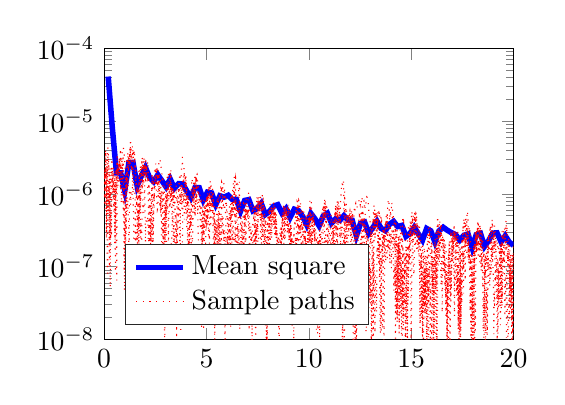
\begin{tikzpicture}

% \begin{axis}[%
% width=5.706cm,
% height=4cm,
% at={(0cm,0cm)},
% scale only axis,
% xmin=0,
% xmax=20,
% ymode=log,
% ymin=1e-10,
% ymax=0.0001,
% yminorticks=true,
% axis background/.style={fill=white},
% title style={font=\bfseries},
% title={error closed-loop system},
% legend style={legend cell align=left, align=left, draw=white!15!black}
% ]
\begin{axis}[%
width=5.2cm,
height=3.7cm,
at={(0cm,0cm)},
scale only axis,
xmin=0,
xmax=20,
ymin=1e-08,
ymax=1e-4,
ymode=log,
axis background/.style={fill=white},
legend style={at={(0.05,0.05)}, anchor=south west, legend cell align=left, align=left, draw=white!15!black}
]
\addplot [color=blue, line width=2.0pt]
  table[row sep=crcr]{%
0	0\\
0.202020202020202	4.07824277542804e-05\\
0.404040404040404	8.00555258100639e-06\\
0.606060606060606	1.93760639604469e-06\\
0.808080808080808	1.93626355437312e-06\\
1.01010101010101	1.10927778505979e-06\\
1.21212121212121	2.67550582165818e-06\\
1.41414141414141	2.69573101595518e-06\\
1.61616161616162	1.28430708841694e-06\\
1.81818181818182	1.7537503192262e-06\\
2.02020202020202	2.298227294745e-06\\
2.22222222222222	1.67283018762468e-06\\
2.42424242424242	1.47292626746642e-06\\
2.62626262626263	1.82436217013951e-06\\
2.82828282828283	1.51316151527027e-06\\
3.03030303030303	1.24325014726355e-06\\
3.23232323232323	1.5937056387878e-06\\
3.43434343434343	1.19363000835037e-06\\
3.63636363636364	1.37712267673274e-06\\
3.83838383838384	1.37178801120339e-06\\
4.04040404040404	1.09248048355853e-06\\
4.24242424242424	8.89943439800062e-07\\
4.44444444444444	1.22045101943362e-06\\
4.64646464646465	1.21352340310808e-06\\
4.84848484848485	8.22982758799756e-07\\
5.05050505050505	1.0549128428619e-06\\
5.25252525252525	1.02734352318636e-06\\
5.45454545454545	7.14253275908181e-07\\
5.65656565656566	9.4136590039811e-07\\
5.85858585858586	8.99997408546679e-07\\
6.06060606060606	9.55484160165764e-07\\
6.26262626262626	8.36800036841001e-07\\
6.46464646464646	8.35819503333777e-07\\
6.66666666666667	5.77394478669719e-07\\
6.86868686868687	8.10410295767769e-07\\
7.07070707070707	8.33028503383415e-07\\
7.27272727272727	5.86332159889176e-07\\
7.47474747474747	6.31452693043457e-07\\
7.67676767676768	7.40078195657773e-07\\
7.87878787878788	5.20654034214867e-07\\
8.08080808080808	5.72610651785131e-07\\
8.28282828282828	6.78707159602533e-07\\
8.48484848484848	7.09583435445949e-07\\
8.68686868686869	5.45281449667405e-07\\
8.88888888888889	6.29018712984296e-07\\
9.09090909090909	4.74478564969311e-07\\
9.29292929292929	6.1425888236521e-07\\
9.49494949494949	5.88612891584862e-07\\
9.6969696969697	4.92319164123579e-07\\
9.8989898989899	3.75019037236162e-07\\
10.1010101010101	5.3944653546908e-07\\
10.3030303030303	4.53100899356122e-07\\
10.5050505050505	3.64566684016713e-07\\
10.7070707070707	4.96836709921461e-07\\
10.9090909090909	5.41262988476621e-07\\
11.1111111111111	3.95338989604672e-07\\
11.3131313131313	4.5455681277475e-07\\
11.5151515151515	4.32086076211196e-07\\
11.7171717171717	5.01276230164971e-07\\
11.9191919191919	4.37050079121951e-07\\
12.1212121212121	4.33599379434e-07\\
12.3232323232323	2.64267263029737e-07\\
12.5252525252525	3.91238316036081e-07\\
12.7272727272727	4.08762591660682e-07\\
12.9292929292929	2.86602995429285e-07\\
13.1313131313131	3.44206481382708e-07\\
13.3333333333333	4.20190053116888e-07\\
13.5353535353535	3.34613135965317e-07\\
13.7373737373737	3.12158564433459e-07\\
13.9393939393939	3.81951510936981e-07\\
14.1414141414141	4.18078483020565e-07\\
14.3434343434343	3.55228280033925e-07\\
14.5454545454545	3.6839304828036e-07\\
14.7474747474747	2.60275372449399e-07\\
14.9494949494949	2.87455213024794e-07\\
15.1515151515152	3.48552794160172e-07\\
15.3535353535354	2.81153935744178e-07\\
15.5555555555556	2.31653884196773e-07\\
15.7575757575758	3.3414682265317e-07\\
15.959595959596	3.10477568652845e-07\\
16.1616161616162	2.18434929517447e-07\\
16.3636363636364	3.10537907685651e-07\\
16.5656565656566	3.47719801249642e-07\\
16.7676767676768	3.1614003509172e-07\\
16.969696969697	2.92622670080726e-07\\
17.1717171717172	2.75087073191094e-07\\
17.3737373737374	2.31266436911998e-07\\
17.5757575757576	2.69295967792273e-07\\
17.7777777777778	2.8107403443483e-07\\
17.979797979798	1.82272874038578e-07\\
18.1818181818182	2.75579673055555e-07\\
18.3838383838384	2.87038250053927e-07\\
18.5858585858586	1.89908937808278e-07\\
18.7878787878788	2.27942017645268e-07\\
18.989898989899	2.88883718737907e-07\\
19.1919191919192	2.9151644517401e-07\\
19.3939393939394	2.19226219847825e-07\\
19.5959595959596	2.65507127683619e-07\\
19.7979797979798	2.1588854522371e-07\\
20	1.96511712009889e-07\\
};
\addlegendentry{Mean square}

\addplot [color=red, dotted]
  table[row sep=crcr]{%
0	0\\
0.02002002002002	1.79738231652466e-06\\
0.04004004004004	6.11166875139531e-07\\
0.0600600600600601	1.13343033125576e-06\\
0.0800800800800801	2.58472336390318e-06\\
0.1001001001001	1.31203014942339e-06\\
0.12012012012012	2.9517715493227e-07\\
0.14014014014014	2.10126522674471e-06\\
0.16016016016016	2.30006788739547e-06\\
0.18018018018018	5.63992547635216e-07\\
0.2002002002002	1.46098105193566e-06\\
0.22022022022022	1.58349127143162e-06\\
0.24024024024024	9.39293444193072e-07\\
0.26026026026026	6.88291735954725e-07\\
0.28028028028028	1.4121050841941e-06\\
0.3003003003003	1.41862685001988e-06\\
0.32032032032032	1.30408883079514e-06\\
0.34034034034034	2.31513883624311e-06\\
0.36036036036036	2.01575195958695e-06\\
0.38038038038038	1.83771377090803e-06\\
0.4004004004004	1.75106818859878e-06\\
0.42042042042042	1.00614243793669e-06\\
0.44044044044044	8.87847094816436e-07\\
0.46046046046046	1.48319207543437e-06\\
0.48048048048048	1.73331391815283e-06\\
0.500500500500501	1.11178366037768e-06\\
0.520520520520521	1.73743301952242e-07\\
0.540540540540541	8.12037832710451e-07\\
0.560560560560561	7.07434773441614e-07\\
0.580580580580581	1.38597234438932e-06\\
0.600600600600601	9.9584773550479e-07\\
0.620620620620621	1.94322076274113e-06\\
0.640640640640641	2.25882721486134e-06\\
0.660660660660661	2.17012984119678e-06\\
0.680680680680681	2.07670736186002e-06\\
0.700700700700701	2.15484419813164e-06\\
0.720720720720721	1.37937588506534e-06\\
0.740740740740741	1.50985710411764e-06\\
0.760760760760761	1.54472496073403e-06\\
0.780780780780781	1.57753705089512e-06\\
0.800800800800801	1.28471887729001e-06\\
0.820820820820821	1.36711221597343e-06\\
0.840840840840841	7.36712284666624e-07\\
0.860860860860861	9.36969242900545e-07\\
0.880880880880881	1.61165931084056e-06\\
0.900900900900901	1.45876281664707e-06\\
0.920920920920921	3.41202629409401e-06\\
0.940940940940941	2.95543056364151e-06\\
0.960960960960961	1.60093331528921e-06\\
0.980980980980981	1.65864568692186e-06\\
1.001001001001	1.29724967007081e-06\\
1.02102102102102	8.6272563023945e-07\\
1.04104104104104	1.24012425932804e-07\\
1.06106106106106	3.70730654210053e-07\\
1.08108108108108	5.45277473565259e-07\\
1.1011011011011	1.96637556023943e-06\\
1.12112112112112	1.46254931495283e-06\\
1.14114114114114	1.08375857167848e-06\\
1.16116116116116	1.67394000719144e-06\\
1.18118118118118	1.24544452152292e-06\\
1.2012012012012	2.92763368422675e-06\\
1.22122122122122	2.64741230376142e-06\\
1.24124124124124	3.78175339354213e-06\\
1.26126126126126	2.40397859544669e-06\\
1.28128128128128	3.01057404036537e-06\\
1.3013013013013	3.40947295880296e-06\\
1.32132132132132	2.55609229696073e-06\\
1.34134134134134	2.05238454975593e-06\\
1.36136136136136	2.3241113666785e-06\\
1.38138138138138	2.29028943695376e-06\\
1.4014014014014	1.65565234493621e-06\\
1.42142142142142	8.02593044699843e-07\\
1.44144144144144	5.14396169731401e-07\\
1.46146146146146	2.21149343265277e-08\\
1.48148148148148	1.31011244218081e-07\\
1.5015015015015	1.16274652188354e-07\\
1.52152152152152	5.54479535734012e-07\\
1.54154154154154	1.15250030139807e-07\\
1.56156156156156	6.86948085867038e-08\\
1.58158158158158	4.60394116476129e-08\\
1.6016016016016	2.372195322979e-08\\
1.62162162162162	3.40010973291381e-07\\
1.64164164164164	5.82036732248516e-07\\
1.66166166166166	6.3329940774291e-07\\
1.68168168168168	3.33272810945815e-07\\
1.7017017017017	7.59899828274655e-07\\
1.72172172172172	3.07079519780806e-07\\
1.74174174174174	2.1945463953696e-06\\
1.76176176176176	6.641353395715e-07\\
1.78178178178178	6.8797089129196e-07\\
1.8018018018018	1.54923040086651e-06\\
1.82182182182182	2.0310315350374e-06\\
1.84184184184184	2.8107727145543e-06\\
1.86186186186186	1.18686229737275e-06\\
1.88188188188188	1.71292505713927e-06\\
1.9019019019019	2.72462269009781e-06\\
1.92192192192192	2.73387237835817e-06\\
1.94194194194194	1.41638860719469e-06\\
1.96196196196196	1.99629608563945e-06\\
1.98198198198198	2.4497555747375e-06\\
2.002002002002	1.78761448546649e-06\\
2.02202202202202	2.71506553095908e-06\\
2.04204204204204	2.24006075381222e-06\\
2.06206206206206	1.69213244835192e-06\\
2.08208208208208	2.18496928395914e-06\\
2.1021021021021	2.66960116596166e-06\\
2.12212212212212	2.5696135574795e-06\\
2.14214214214214	2.8108157150485e-06\\
2.16216216216216	1.81914102200669e-06\\
2.18218218218218	1.32079774699328e-06\\
2.2022022022022	1.22157639720319e-06\\
2.22222222222222	9.46901798265708e-07\\
2.24224224224224	7.07155873781529e-07\\
2.26226226226226	4.63206624386493e-07\\
2.28228228228228	2.08689823920761e-08\\
2.3023023023023	4.60271794451449e-07\\
2.32232232232232	4.25641298291139e-07\\
2.34234234234234	9.5921218816757e-07\\
2.36236236236236	9.19874128275405e-07\\
2.38238238238238	1.32163010759813e-06\\
2.4024024024024	1.35836333145153e-06\\
2.42242242242242	1.47885384423337e-06\\
2.44244244244244	1.43876562546459e-06\\
2.46246246246246	1.76048988948283e-06\\
2.48248248248248	1.74727368466441e-06\\
2.5025025025025	2.24320704979682e-06\\
2.52252252252252	2.18527418459989e-06\\
2.54254254254254	2.08426428641142e-06\\
2.56256256256256	1.99457952571198e-06\\
2.58258258258258	2.30278332307856e-06\\
2.6026026026026	1.74976830545487e-06\\
2.62262262262262	1.76072725556906e-06\\
2.64264264264264	2.20236009367197e-06\\
2.66266266266266	2.4561928693631e-06\\
2.68268268268268	2.69943092608889e-06\\
2.7027027027027	2.79537436446585e-06\\
2.72272272272272	3.00187885759723e-06\\
2.74274274274274	2.91294068847336e-06\\
2.76276276276276	2.38102166843405e-06\\
2.78278278278278	2.33017858112856e-06\\
2.8028028028028	2.02445883307823e-06\\
2.82282282282282	1.97998164658418e-06\\
2.84284284284284	1.53828080270741e-06\\
2.86286286286286	1.74930811800336e-06\\
2.88288288288288	7.5134123223183e-07\\
2.9029029029029	1.08495086130117e-06\\
2.92292292292292	1.12037251692603e-06\\
2.94294294294294	1.26722790174018e-06\\
2.96296296296296	4.21956351280248e-07\\
2.98298298298298	2.48219692178912e-07\\
3.003003003003	1.03577217881477e-06\\
3.02302302302302	9.22752268021462e-07\\
3.04304304304304	3.93653680711009e-07\\
3.06306306306306	7.26016120220963e-08\\
3.08308308308308	1.26160413290499e-07\\
3.1031031031031	1.25185940561762e-07\\
3.12312312312312	4.86588518315045e-08\\
3.14314314314314	2.95131318892765e-07\\
3.16316316316316	1.81709232431114e-07\\
3.18318318318318	1.75483323845342e-07\\
3.2032032032032	9.56110172835112e-08\\
3.22322322322322	8.4921522182168e-08\\
3.24324324324324	1.82983651575213e-07\\
3.26326326326326	1.23898342716926e-07\\
3.28328328328328	2.14968149124457e-07\\
3.3033033033033	2.12947128259638e-07\\
3.32332332332332	3.70072516875946e-07\\
3.34334334334334	8.043514561559e-07\\
3.36336336336336	1.00607246697146e-06\\
3.38338338338338	7.50328663576051e-07\\
3.4034034034034	7.86899118728879e-07\\
3.42342342342342	1.02424102910186e-06\\
3.44344344344344	7.42469467629628e-07\\
3.46346346346346	8.45034463317032e-07\\
3.48348348348348	8.56879854356721e-07\\
3.5035035035035	9.64043087057155e-07\\
3.52352352352352	1.3116327785357e-06\\
3.54354354354354	8.54098135293191e-07\\
3.56356356356356	9.45667413017613e-07\\
3.58358358358358	8.76339278050685e-07\\
3.6036036036036	9.71790876020393e-07\\
3.62362362362362	1.26141853894396e-06\\
3.64364364364364	1.40173588571157e-06\\
3.66366366366366	1.01425578258423e-06\\
3.68368368368368	1.67776718179388e-06\\
3.7037037037037	1.87872755570783e-06\\
3.72372372372372	1.55950283485649e-06\\
3.74374374374374	1.6318527970512e-06\\
3.76376376376376	1.6884116475164e-06\\
3.78378378378378	2.24986473285356e-06\\
3.8038038038038	2.20602160707234e-06\\
3.82382382382382	3.20427646601295e-06\\
3.84384384384384	2.35657026089956e-06\\
3.86386386386386	2.34022159852947e-06\\
3.88388388388388	2.25356137421942e-06\\
3.9039039039039	2.28789203197301e-06\\
3.92392392392392	1.65031864964e-06\\
3.94394394394394	1.67595544483991e-06\\
3.96396396396396	1.7366035729545e-06\\
3.98398398398398	1.15840478191725e-06\\
4.004004004004	1.55906397196905e-06\\
4.02402402402402	1.14587909376062e-06\\
4.04404404404404	8.00279897316302e-07\\
4.06406406406406	8.47546500164415e-07\\
4.08408408408408	6.73745125203159e-07\\
4.1041041041041	9.19572516827081e-07\\
4.12412412412412	7.061112426686e-07\\
4.14414414414414	3.87524725039024e-07\\
4.16416416416416	2.39169542963828e-07\\
4.18418418418418	1.80726659900963e-07\\
4.2042042042042	1.67022395600239e-07\\
4.22422422422422	1.25953270310434e-07\\
4.24424424424424	2.12615176186033e-08\\
4.26426426426426	4.5158552269675e-07\\
4.28428428428428	5.23767702664872e-07\\
4.3043043043043	4.07518922515943e-07\\
4.32432432432432	5.62279626818355e-07\\
4.34434434434434	1.05031402618675e-06\\
4.36436436436436	1.14601934500008e-06\\
4.38438438438438	7.85936361378243e-07\\
4.4044044044044	7.52952382899054e-07\\
4.42442442442442	6.54243346926827e-07\\
4.44444444444444	5.29284082005065e-07\\
4.46446446446446	6.22757610750025e-07\\
4.48448448448448	7.1006840206737e-07\\
4.5045045045045	9.05704560490301e-07\\
4.52452452452452	9.44190469913991e-07\\
4.54454454454454	8.67293200997257e-07\\
4.56456456456456	6.88741881928096e-07\\
4.58458458458458	5.52126477997668e-07\\
4.6046046046046	7.37309169337448e-07\\
4.62462462462462	7.99507314492756e-07\\
4.64464464464464	7.40925433470376e-07\\
4.66466466466466	6.44041009668856e-07\\
4.68468468468468	6.21521114774661e-07\\
4.7047047047047	3.2385904824102e-07\\
4.72472472472472	3.27833512729375e-07\\
4.74474474474474	4.45012676717904e-07\\
4.76476476476476	3.6976699883816e-07\\
4.78478478478478	1.54137840227271e-07\\
4.8048048048048	5.39345948729583e-08\\
4.82482482482482	2.22289991419707e-07\\
4.84484484484484	3.94646861709132e-07\\
4.86486486486486	2.1757041021962e-07\\
4.88488488488488	3.05602094336747e-07\\
4.9049049049049	3.61691728813579e-07\\
4.92492492492492	6.01621543173963e-07\\
4.94494494494494	5.52309638566028e-07\\
4.96496496496496	6.42356649975487e-07\\
4.98498498498498	6.21696283806475e-07\\
5.00500500500501	7.05409923324401e-07\\
5.02502502502503	3.92471153241042e-07\\
5.04504504504505	4.20669040292473e-07\\
5.06506506506507	7.85929294483827e-07\\
5.08508508508509	6.69842548594238e-07\\
5.10510510510511	5.58767437569431e-07\\
5.12512512512513	6.99880857145979e-07\\
5.14514514514515	6.28823816445429e-07\\
5.16516516516517	6.65093006327374e-07\\
5.18518518518519	8.57391499841682e-07\\
5.20520520520521	8.17545891045623e-07\\
5.22522522522523	7.08822279108021e-07\\
5.24524524524525	6.41983789873723e-07\\
5.26526526526527	8.04649090251375e-07\\
5.28528528528529	7.9209300025896e-07\\
5.30530530530531	7.35658815459342e-07\\
5.32532532532533	5.97430035955782e-07\\
5.34534534534535	5.05067239558482e-07\\
5.36536536536537	5.85013085020655e-07\\
5.38538538538539	4.41969847885951e-07\\
5.40540540540541	4.74159290164212e-09\\
5.42542542542543	2.77160740555534e-07\\
5.44544544544545	2.71000707410401e-07\\
5.46546546546547	4.12569588271545e-07\\
5.48548548548549	4.31424253428249e-07\\
5.50550550550551	7.5369990246105e-07\\
5.52552552552553	8.22180105482111e-07\\
5.54554554554555	7.58496959690518e-07\\
5.56556556556557	8.94860885176443e-07\\
5.58558558558559	7.75156641137355e-07\\
5.60560560560561	7.82395127911638e-07\\
5.62562562562563	8.00018399467214e-07\\
5.64564564564565	9.99104413410741e-07\\
5.66566566566567	8.7842700273352e-07\\
5.68568568568569	1.00859928990804e-06\\
5.70570570570571	1.07542196617164e-06\\
5.72572572572573	1.10967682756352e-06\\
5.74574574574575	1.06984434868678e-06\\
5.76576576576577	1.21392401652931e-06\\
5.78578578578579	8.23499086229489e-07\\
5.80580580580581	1.08496151991417e-06\\
5.82582582582583	9.94920127154607e-07\\
5.84584584584585	8.93547689893631e-07\\
5.86586586586587	1.08803429299948e-06\\
5.88588588588589	8.78667544687591e-07\\
5.90590590590591	9.09606108887326e-07\\
5.92592592592593	9.11278119165028e-07\\
5.94594594594595	9.68433105458304e-07\\
5.96596596596597	8.63734724882283e-07\\
5.98598598598599	6.69912396099551e-07\\
6.00600600600601	6.28091246954813e-07\\
6.02602602602603	4.84636037042672e-07\\
6.04604604604605	4.08727208854712e-07\\
6.06606606606607	4.5841481226966e-07\\
6.08608608608609	3.05960870639674e-07\\
6.10610610610611	2.19027542678674e-07\\
6.12612612612613	2.61652325246094e-07\\
6.14614614614615	7.12434522384771e-08\\
6.16616616616617	3.60663318873197e-08\\
6.18618618618619	1.47111934929948e-08\\
6.20620620620621	2.08987866433552e-08\\
6.22622622622623	8.59264323208114e-08\\
6.24624624624625	2.80924456674406e-07\\
6.26626626626627	1.44276147031419e-07\\
6.28628628628629	2.20586612150529e-07\\
6.30630630630631	3.69085285006208e-07\\
6.32632632632633	2.22818431235917e-07\\
6.34634634634635	2.12823485076222e-07\\
6.36636636636637	2.29460957623877e-07\\
6.38638638638639	2.94033574269353e-07\\
6.40640640640641	2.50271598434822e-07\\
6.42642642642643	2.39622232538218e-07\\
6.44644644644645	1.79060790167865e-07\\
6.46646646646647	3.16030551588677e-08\\
6.48648648648649	2.03482304942523e-07\\
6.50650650650651	3.71113711163793e-07\\
6.52652652652653	1.73387613874439e-07\\
6.54654654654655	8.35645173415755e-08\\
6.56656656656657	2.12495100803475e-08\\
6.58658658658659	3.46066248736538e-07\\
6.60660660660661	1.53882353194024e-07\\
6.62662662662663	1.35787139914898e-08\\
6.64664664664665	2.23965774006104e-08\\
6.66666666666667	1.82452583802027e-07\\
6.68668668668669	2.29272649084711e-07\\
6.70670670670671	4.27978623274279e-08\\
6.72672672672673	2.70128972949829e-07\\
6.74674674674675	4.81632019629514e-07\\
6.76676676676677	4.79302646069182e-07\\
6.78678678678679	4.714468912802e-07\\
6.80680680680681	8.27940365500653e-07\\
6.82682682682683	6.12924376538818e-07\\
6.84684684684685	4.36912431430813e-07\\
6.86686686686687	5.79745332865785e-07\\
6.88688688688689	8.05650230500459e-07\\
6.90690690690691	7.72587472534059e-07\\
6.92692692692693	7.0609417876177e-07\\
6.94694694694695	8.72013097917092e-07\\
6.96696696696697	7.20576811408762e-07\\
6.98698698698699	6.60720963903323e-07\\
7.00700700700701	6.81157634640336e-07\\
7.02702702702703	6.53121800063223e-07\\
7.04704704704705	9.43913475673555e-07\\
7.06706706706707	1.05707972371504e-06\\
7.08708708708709	1.05193606926327e-06\\
7.10710710710711	9.15660379895055e-07\\
7.12712712712713	8.22905180530973e-07\\
7.14714714714715	8.11005344354561e-07\\
7.16716716716717	6.3571347998283e-07\\
7.18718718718719	6.91498233964351e-07\\
7.20720720720721	6.80432886611471e-07\\
7.22722722722723	6.67418346595122e-07\\
7.24724724724725	5.29846363338105e-07\\
7.26726726726727	5.52627542453117e-07\\
7.28728728728729	6.92980559523387e-07\\
7.30730730730731	5.92693263370743e-07\\
7.32732732732733	5.46152524731795e-07\\
7.34734734734735	3.89329344704832e-07\\
7.36736736736737	2.10072182826426e-07\\
7.38738738738739	3.7774043935791e-07\\
7.40740740740741	2.24723644311747e-07\\
7.42742742742743	1.62922076494578e-07\\
7.44744744744745	4.00076462256001e-08\\
7.46746746746747	1.60051285965374e-07\\
7.48748748748749	5.64668652618152e-08\\
7.50750750750751	2.32050104540784e-07\\
7.52752752752753	2.88987341063929e-07\\
7.54754754754755	1.98107933300496e-07\\
7.56756756756757	6.14635910083292e-08\\
7.58758758758759	3.35282684008541e-08\\
7.60760760760761	4.8914861385947e-08\\
7.62762762762763	2.1449086010826e-07\\
7.64764764764765	4.55406601212524e-07\\
7.66766766766767	3.45743741363654e-07\\
7.68768768768769	2.01876726173413e-07\\
7.70770770770771	4.18675647925059e-07\\
7.72772772772773	6.80617829726547e-07\\
7.74774774774775	6.56989165268112e-07\\
7.76776776776777	5.25009324052707e-07\\
7.78778778778779	4.36372514987606e-07\\
7.80780780780781	4.53209174443027e-07\\
7.82782782782783	2.71644831424221e-07\\
7.84784784784785	1.54689912259424e-07\\
7.86786786786787	2.05170291817289e-07\\
7.88788788788789	1.33005179864414e-07\\
7.90790790790791	2.35622119401297e-07\\
7.92792792792793	6.09547606688193e-08\\
7.94794794794795	9.05367489958121e-09\\
7.96796796796797	3.09489793978417e-08\\
7.98798798798799	2.13554997874344e-07\\
8.00800800800801	7.91447102350976e-08\\
8.02802802802803	2.61883144624364e-07\\
8.04804804804805	5.77949173307755e-07\\
8.06806806806807	3.43402976016245e-07\\
8.08808808808809	5.78588888135684e-07\\
8.10810810810811	7.24631910986496e-07\\
8.12812812812813	5.55866654341903e-07\\
8.14814814814815	5.46115042466198e-07\\
8.16816816816817	6.3512816882322e-07\\
8.18818818818819	6.24620135735298e-07\\
8.20820820820821	5.55545111578682e-07\\
8.22822822822823	6.49548028099954e-07\\
8.24824824824825	5.07130766595783e-07\\
8.26826826826827	3.60343643808604e-07\\
8.28828828828829	4.60121746930037e-07\\
8.30830830830831	4.0963418119535e-07\\
8.32832832832833	3.56630681282304e-07\\
8.34834834834835	4.62988989627622e-07\\
8.36836836836837	4.72818286918893e-07\\
8.38838838838839	3.95716401691783e-07\\
8.40840840840841	2.57205638329745e-07\\
8.42842842842843	2.2372704031607e-07\\
8.44844844844845	1.76104570359004e-07\\
8.46846846846847	1.95726221999464e-07\\
8.48848848848849	1.21872932962923e-07\\
8.50850850850851	1.11219580203389e-07\\
8.52852852852853	6.23266160748905e-08\\
8.54854854854855	8.93542305031299e-08\\
8.56856856856857	3.55962481937389e-08\\
8.58858858858859	7.55608881677652e-08\\
8.60860860860861	1.28741004469896e-07\\
8.62862862862863	2.22376995080162e-07\\
8.64864864864865	2.26528252081621e-07\\
8.66866866866867	2.30818300520315e-07\\
8.68868868868869	2.77540802601587e-07\\
8.70870870870871	3.25011456433092e-07\\
8.72872872872873	5.23010668376231e-07\\
8.74874874874875	3.54002618118938e-07\\
8.76876876876877	2.90130749838245e-07\\
8.78878878878879	4.33234265488594e-07\\
8.80880880880881	5.67265281871284e-07\\
8.82882882882883	4.89424674388493e-07\\
8.84884884884885	4.79903777359641e-07\\
8.86886886886887	4.65587733580272e-07\\
8.88888888888889	5.37348795306696e-07\\
8.90890890890891	3.56616957636492e-07\\
8.92892892892893	3.70294207279854e-07\\
8.94894894894895	3.70912916082932e-07\\
8.96896896896897	4.73570446938744e-07\\
8.98898898898899	4.09468597957851e-07\\
9.00900900900901	3.16689360912027e-07\\
9.02902902902903	2.21682174187003e-07\\
9.04904904904905	3.32666671030617e-07\\
9.06906906906907	3.97576571108203e-07\\
9.08908908908909	2.37673016250087e-07\\
9.10910910910911	3.79485871317571e-07\\
9.12912912912913	3.3848519643712e-07\\
9.14914914914915	2.74931589251076e-07\\
9.16916916916917	2.43251981518509e-07\\
9.18918918918919	6.03326405132564e-08\\
9.20920920920921	9.39427520316847e-08\\
9.22922922922923	3.37974017169889e-08\\
9.24924924924925	3.00685020837357e-08\\
9.26926926926927	7.34584231396471e-09\\
9.28928928928929	8.89316884435943e-08\\
9.30930930930931	6.98194081352501e-08\\
9.32932932932933	8.9470002078355e-08\\
9.34934934934935	1.49929097132198e-08\\
9.36936936936937	4.29280650116133e-08\\
9.38938938938939	1.26615877126397e-07\\
9.40940940940941	2.4853988768114e-07\\
9.42942942942943	1.59430799900862e-07\\
9.44944944944945	3.03177395378309e-07\\
9.46946946946947	7.54234167142967e-07\\
9.48948948948949	3.19561142458192e-07\\
9.50950950950951	3.45353263673718e-07\\
9.52952952952953	3.04774899630482e-07\\
9.54954954954955	4.83133299092281e-07\\
9.56956956956957	4.76538461479968e-07\\
9.58958958958959	3.80157996735921e-07\\
9.60960960960961	2.46724254165292e-07\\
9.62962962962963	2.84089744423174e-07\\
9.64964964964965	2.08204758827112e-07\\
9.66966966966967	2.17557271433342e-07\\
9.68968968968969	8.31013533751741e-08\\
9.70970970970971	5.97722751947577e-08\\
9.72972972972973	1.42487159998622e-07\\
9.74974974974975	2.73037742140413e-08\\
9.76976976976977	9.09419050275975e-08\\
9.78978978978979	8.08355792777694e-08\\
9.80980980980981	2.94769519565409e-07\\
9.82982982982983	2.97537977726574e-07\\
9.84984984984985	1.45396090213323e-07\\
9.86986986986987	2.28557515606712e-07\\
9.88988988988989	1.68674125574107e-07\\
9.90990990990991	1.57309098870777e-07\\
9.92992992992993	3.24024065642337e-08\\
9.94994994994995	2.71990140857065e-08\\
9.96996996996997	1.77998418139442e-07\\
9.98998998998999	2.36060514754875e-07\\
10.01001001001	3.62603535429979e-07\\
10.03003003003	1.89574780452062e-07\\
10.0500500500501	2.83162363272415e-07\\
10.0700700700701	6.62530501624224e-07\\
10.0900900900901	3.27186621703728e-07\\
10.1101101101101	1.86115361791696e-07\\
10.1301301301301	3.07077809953834e-07\\
10.1501501501502	2.1985737590093e-07\\
10.1701701701702	4.25326377824192e-07\\
10.1901901901902	2.37837144886243e-07\\
10.2102102102102	1.59892081054493e-07\\
10.2302302302302	2.10860665296596e-07\\
10.2502502502503	1.1582698072359e-07\\
10.2702702702703	3.46441879987803e-08\\
10.2902902902903	4.93502474462582e-08\\
10.3103103103103	3.00931082323783e-08\\
10.3303303303303	3.46138441803678e-08\\
10.3503503503504	6.60247057921834e-08\\
10.3703703703704	7.09176548917808e-08\\
10.3903903903904	4.4004078080359e-08\\
10.4104104104104	2.21746317004246e-07\\
10.4304304304304	3.57841742483747e-08\\
10.4504504504505	9.3273075386992e-08\\
10.4704704704705	2.37888520660381e-07\\
10.4904904904905	1.52366057252898e-07\\
10.5105105105105	1.17727525231837e-07\\
10.5305305305305	2.91730324480333e-07\\
10.5505505505506	3.18507069019212e-07\\
10.5705705705706	4.93439550318586e-07\\
10.5905905905906	3.86162992960011e-07\\
10.6106106106106	3.71332112146889e-07\\
10.6306306306306	3.92115382848579e-07\\
10.6506506506507	5.44372166202902e-07\\
10.6706706706707	6.39460894137846e-07\\
10.6906906906907	5.02247281393232e-07\\
10.7107107107107	7.15770708545298e-07\\
10.7307307307307	4.78632265384813e-07\\
10.7507507507508	4.87396374955691e-07\\
10.7707707707708	6.53441488405021e-07\\
10.7907907907908	7.10140917536171e-07\\
10.8108108108108	5.94979772563134e-07\\
10.8308308308308	5.30772366186925e-07\\
10.8508508508509	4.4438810990427e-07\\
10.8708708708709	3.98477192656646e-07\\
10.8908908908909	3.53625968945752e-07\\
10.9109109109109	3.14404239283938e-07\\
10.9309309309309	2.51099571413463e-07\\
10.950950950951	2.06402432529122e-07\\
10.970970970971	1.67151152782826e-07\\
10.990990990991	1.78306591406588e-07\\
11.011011011011	3.9913998982725e-08\\
11.031031031031	1.08435791817381e-07\\
11.0510510510511	1.64128159177715e-07\\
11.0710710710711	1.04764099671468e-07\\
11.0910910910911	2.17755441085939e-08\\
11.1111111111111	9.52381282999937e-08\\
11.1311311311311	7.89954830421407e-08\\
11.1511511511512	2.03414303365718e-07\\
11.1711711711712	5.39931536677117e-08\\
11.1911911911912	2.73080582052352e-07\\
11.2112112112112	3.50742045626391e-07\\
11.2312312312312	5.15986521455905e-08\\
11.2512512512513	4.03686798017927e-07\\
11.2712712712713	5.88085649875657e-07\\
11.2912912912913	4.68192304077368e-07\\
11.3113113113113	7.22485940971809e-07\\
11.3313313313313	5.38573098493046e-07\\
11.3513513513514	5.52545038704746e-07\\
11.3713713713714	6.06393978938516e-07\\
11.3913913913914	7.86936403232749e-07\\
11.4114114114114	4.97588540236325e-07\\
11.4314314314314	4.77527773978249e-07\\
11.4514514514515	4.12781783378686e-07\\
11.4714714714715	3.60808949303907e-07\\
11.4914914914915	3.27715376600675e-07\\
11.5115115115115	2.5117547448251e-07\\
11.5315315315315	3.01499495570882e-07\\
11.5515515515516	1.91795736670561e-07\\
11.5715715715716	1.06899190126047e-07\\
11.5915915915916	1.02792797925289e-07\\
11.6116116116116	3.16521660752372e-08\\
11.6316316316316	1.82980757484416e-08\\
11.6516516516517	2.69583185274076e-09\\
11.6716716716717	9.57665778338654e-08\\
11.6916916916917	1.24534866480925e-07\\
11.7117117117117	3.78545927924215e-08\\
11.7317317317317	7.68878315605985e-08\\
11.7517517517518	1.89080419297562e-07\\
11.7717717717718	1.08155188870387e-07\\
11.7917917917918	9.17388863315817e-08\\
11.8118118118118	1.52847068051572e-08\\
11.8318318318318	1.68908221714528e-07\\
11.8518518518519	3.95331169023656e-07\\
11.8718718718719	3.75226350301616e-07\\
11.8918918918919	1.0040903252457e-07\\
11.9119119119119	2.39765336025069e-07\\
11.9319319319319	2.83059079225156e-07\\
11.951951951952	4.45884083126916e-07\\
11.971971971972	4.80118111802019e-07\\
11.991991991992	5.02992719137286e-07\\
12.012012012012	4.61759668144532e-07\\
12.032032032032	2.85411198843925e-07\\
12.0520520520521	2.19469969748836e-07\\
12.0720720720721	2.53174335385779e-07\\
12.0920920920921	2.35320321031163e-07\\
12.1121121121121	1.60274709924248e-07\\
12.1321321321321	3.13520234453494e-07\\
12.1521521521522	2.86570539933627e-07\\
12.1721721721722	2.97581657936243e-07\\
12.1921921921922	2.54938699377573e-07\\
12.2122122122122	2.81023589104182e-07\\
12.2322322322322	2.92836321215879e-07\\
12.2522522522523	4.05925197598477e-07\\
12.2722722722723	1.00820264522272e-08\\
12.2922922922923	3.26813490145769e-07\\
12.3123123123123	2.30687669873458e-07\\
12.3323323323323	1.69347502325613e-07\\
12.3523523523524	1.271290087932e-07\\
12.3723723723724	8.26824662410753e-08\\
12.3923923923924	1.01886512811349e-07\\
12.4124124124124	1.16368478056111e-07\\
12.4324324324324	6.85813284446888e-08\\
12.4524524524525	7.65929546275135e-08\\
12.4724724724725	3.8799492175762e-08\\
12.4924924924925	2.26101110316716e-08\\
12.5125125125125	1.64365274497768e-07\\
12.5325325325325	6.36402115347063e-08\\
12.5525525525526	2.92444181600082e-07\\
12.5725725725726	7.00428283318718e-08\\
12.5925925925926	3.28965799213185e-07\\
12.6126126126126	4.24492374479904e-07\\
12.6326326326326	2.51117142163164e-07\\
12.6526526526527	2.5208300866903e-07\\
12.6726726726727	2.89322303451814e-07\\
12.6926926926927	3.52451316162531e-07\\
12.7127127127127	2.86520183261809e-07\\
12.7327327327327	4.17362285408774e-08\\
12.7527527527528	1.20229454280609e-07\\
12.7727727727728	1.7728947029071e-07\\
12.7927927927928	1.33689994403353e-08\\
12.8128128128128	1.26045270492745e-08\\
12.8328328328328	5.87008042738406e-08\\
12.8528528528529	2.52527524931829e-08\\
12.8728728728729	9.99912957575201e-08\\
12.8928928928929	8.2838110031273e-08\\
12.9129129129129	1.13438379932458e-07\\
12.9329329329329	1.31715973226758e-07\\
12.952952952953	1.99133171761363e-07\\
12.972972972973	1.89020655592859e-07\\
12.992992992993	2.08558317645216e-07\\
13.013013013013	2.19389928152633e-07\\
13.033033033033	2.98586072340257e-07\\
13.0530530530531	3.03191826282925e-07\\
13.0730730730731	3.33126548396655e-07\\
13.0930930930931	3.35425653709366e-07\\
13.1131131131131	2.77011605467116e-07\\
13.1331331331331	4.57647170102035e-07\\
13.1531531531532	3.45953676304412e-07\\
13.1731731731732	4.39862784055641e-07\\
13.1931931931932	5.86940631224184e-07\\
13.2132132132132	3.71083712940091e-07\\
13.2332332332332	4.35811538606715e-07\\
13.2532532532533	4.56769754744433e-07\\
13.2732732732733	4.95269047902868e-07\\
13.2932932932933	5.55529417144416e-07\\
13.3133133133133	4.8970737429202e-07\\
13.3333333333333	4.54881643780005e-07\\
13.3533533533534	4.06575549271481e-07\\
13.3733733733734	4.62066859516e-07\\
13.3933933933934	3.77421225033663e-07\\
13.4134134134134	3.81458039051071e-07\\
13.4334334334334	3.64849737772459e-07\\
13.4534534534535	1.99989314969998e-07\\
13.4734734734735	1.5519067055955e-07\\
13.4934934934935	1.15957112535996e-07\\
13.5135135135135	8.89571467460927e-08\\
13.5335335335335	1.23502722583339e-07\\
13.5535535535536	4.53682623170139e-08\\
13.5735735735736	2.54165271382942e-08\\
13.5935935935936	1.38602236275125e-08\\
13.6136136136136	2.50950778849135e-08\\
13.6336336336336	9.44210251138412e-08\\
13.6536536536537	1.44315749234661e-07\\
13.6736736736737	1.3332732108244e-07\\
13.6936936936937	1.61833642868923e-07\\
13.7137137137137	1.91810850607115e-07\\
13.7337337337337	2.78438442917251e-07\\
13.7537537537538	2.34389970866625e-07\\
13.7737737737738	2.46259507328498e-07\\
13.7937937937938	1.93966974771886e-07\\
13.8138138138138	1.50725077140385e-07\\
13.8338338338338	1.29426161926697e-07\\
13.8538538538539	1.98416892982317e-07\\
13.8738738738739	1.71032922811153e-07\\
13.8938938938939	2.51339334446379e-07\\
13.9139139139139	2.29590237506982e-07\\
13.9339339339339	1.45987051226968e-07\\
13.953953953954	2.18705061031834e-07\\
13.973973973974	3.08088987077015e-07\\
13.993993993994	3.47263213742915e-07\\
14.014014014014	3.45946578455987e-07\\
14.034034034034	3.50287316565243e-07\\
14.0540540540541	3.52833483552853e-07\\
14.0740740740741	2.37088255987879e-07\\
14.0940940940941	2.26057946742211e-07\\
14.1141141141141	2.03823435340024e-07\\
14.1341341341341	3.21960132714413e-07\\
14.1541541541542	3.22067531273601e-07\\
14.1741741741742	2.05297893032979e-07\\
14.1941941941942	2.040057179458e-07\\
14.2142142142142	1.59375849459715e-07\\
14.2342342342342	5.65920116125442e-08\\
14.2542542542543	5.6845377022048e-08\\
14.2742742742743	8.03028357046884e-08\\
14.2942942942943	2.90449324509675e-08\\
14.3143143143143	1.92976599774928e-07\\
14.3343343343343	1.86849585556194e-08\\
14.3543543543544	2.13532035157875e-08\\
14.3743743743744	2.01875587715117e-07\\
14.3943943943944	1.64073416773578e-07\\
14.4144144144144	1.88416377314931e-07\\
14.4344344344344	9.79889104204305e-08\\
14.4544544544545	3.12712365961191e-07\\
14.4744744744745	3.72507393308866e-07\\
14.4944944944945	2.72921041108256e-07\\
14.5145145145145	2.02394910251366e-07\\
14.5345345345345	1.70406663312858e-07\\
14.5545545545546	1.89321073098126e-07\\
14.5745745745746	4.1576896185191e-07\\
14.5945945945946	4.88334306084939e-07\\
14.6146146146146	3.78022245021588e-07\\
14.6346346346346	4.03566910030908e-07\\
14.6546546546547	3.43224584875e-07\\
14.6746746746747	3.51732282188783e-07\\
14.6946946946947	3.42709426067793e-07\\
14.7147147147147	2.92659409806541e-07\\
14.7347347347347	2.21131912451276e-07\\
14.7547547547548	1.48069580910866e-07\\
14.7747747747748	1.34248116402103e-07\\
14.7947947947948	5.51313014903806e-08\\
14.8148148148148	9.32703181012795e-09\\
14.8348348348348	5.02022467649517e-08\\
14.8548548548549	4.22649653207344e-08\\
14.8748748748749	1.27325056980613e-07\\
14.8948948948949	1.37508542171179e-07\\
14.9149149149149	1.49474345668865e-07\\
14.9349349349349	2.36309934057212e-07\\
14.954954954955	1.91165193610954e-07\\
14.974974974975	1.90353355309665e-07\\
14.994994994995	9.01922679873834e-09\\
15.015015015015	1.91525074163415e-08\\
15.035035035035	9.7720886160513e-08\\
15.0550550550551	3.33270858670052e-07\\
15.0750750750751	2.96347011907176e-07\\
15.0950950950951	2.06172330323198e-07\\
15.1151151151151	2.63202508528255e-07\\
15.1351351351351	2.60605763087576e-07\\
15.1551551551552	3.47214138896172e-07\\
15.1751751751752	2.70773784451237e-07\\
15.1951951951952	3.17109515050147e-07\\
15.2152152152152	2.07646589655574e-07\\
15.2352352352352	2.11038681005141e-07\\
15.2552552552553	2.14197580828882e-07\\
15.2752752752753	1.62415097310348e-07\\
15.2952952952953	1.62468911335314e-07\\
15.3153153153153	2.40673899545869e-07\\
15.3353353353353	2.39699524892887e-07\\
15.3553553553554	1.88127675288534e-07\\
15.3753753753754	2.86768270939669e-07\\
15.3953953953954	1.48463947820022e-07\\
15.4154154154154	6.64647543816122e-08\\
15.4354354354354	1.4308998225724e-08\\
15.4554554554555	2.1623075346783e-08\\
15.4754754754755	2.46963195874858e-08\\
15.4954954954955	1.38716231247351e-07\\
15.5155155155155	2.32876118897012e-08\\
15.5355355355355	8.76077612386087e-08\\
15.5555555555556	1.03328433284746e-07\\
15.5755755755756	9.26595335924447e-08\\
15.5955955955956	1.41601174004549e-07\\
15.6156156156156	1.1212152014862e-07\\
15.6356356356356	1.84727698865029e-07\\
15.6556556556557	1.67413103429539e-07\\
15.6756756756757	1.01488129243223e-07\\
15.6956956956957	4.93950932654154e-08\\
15.7157157157157	4.09958853661005e-08\\
15.7357357357357	3.97944659997426e-08\\
15.7557557557558	2.20295817028719e-08\\
15.7757757757758	4.96604296858064e-08\\
15.7957957957958	2.032934164291e-07\\
15.8158158158158	1.14307734070505e-07\\
15.8358358358358	1.13512688808909e-07\\
15.8558558558559	3.52316940700164e-07\\
15.8758758758759	3.07852264034438e-07\\
15.8958958958959	2.36236566336319e-07\\
15.9159159159159	3.37134158375931e-07\\
15.9359359359359	3.68375019725649e-07\\
15.955955955956	3.38191582753701e-07\\
15.975975975976	2.94110818788508e-07\\
15.995995995996	2.08455827801335e-07\\
16.016016016016	8.61104104334154e-08\\
16.036036036036	7.13045575877687e-08\\
16.0560560560561	5.32562977532866e-08\\
16.0760760760761	5.47109213064756e-08\\
16.0960960960961	6.42470486896425e-08\\
16.1161161161161	4.18442231545829e-08\\
16.1361361361361	1.05511440433747e-07\\
16.1561561561562	1.48123105808303e-07\\
16.1761761761762	1.47004759806202e-07\\
16.1961961961962	1.43849119531531e-07\\
16.2162162162162	2.9623083820408e-07\\
16.2362362362362	2.67240358985964e-07\\
16.2562562562563	2.91303278174404e-07\\
16.2762762762763	3.92193002663822e-07\\
16.2962962962963	4.89555841859042e-07\\
16.3163163163163	3.43721469234451e-07\\
16.3363363363363	2.68258340277698e-07\\
16.3563563563564	3.25318465406853e-07\\
16.3763763763764	4.04855428350643e-07\\
16.3963963963964	4.35257231895739e-07\\
16.4164164164164	3.64828849224712e-07\\
16.4364364364364	3.31570066574026e-07\\
16.4564564564565	2.24349836157974e-07\\
16.4764764764765	3.08191950524977e-07\\
16.4964964964965	2.62118380955719e-07\\
16.5165165165165	2.24158946206622e-07\\
16.5365365365365	2.32767168933241e-07\\
16.5565565565566	2.24970140016491e-07\\
16.5765765765766	2.17099863369547e-07\\
16.5965965965966	1.89736663732131e-07\\
16.6166166166166	1.476984244544e-07\\
16.6366366366366	1.22116764653249e-07\\
16.6566566566567	7.16627458389147e-08\\
16.6766766766767	5.19451531159337e-08\\
16.6966966966967	3.79568641273282e-08\\
16.7167167167167	4.44559934922002e-08\\
16.7367367367367	2.71924367611174e-08\\
16.7567567567568	4.64604205723497e-09\\
16.7767767767768	5.82760836446862e-08\\
16.7967967967968	7.37519552791614e-08\\
16.8168168168168	1.49993272205038e-07\\
16.8368368368368	1.43578748360371e-07\\
16.8568568568569	1.29595253723849e-07\\
16.8768768768769	2.33666667111643e-07\\
16.8968968968969	2.10238919329734e-07\\
16.9169169169169	2.48436399642491e-07\\
16.9369369369369	2.70859976287486e-07\\
16.956956956957	2.22306748072946e-07\\
16.976976976977	2.4699133267476e-07\\
16.996996996997	1.99332563784778e-07\\
17.017017017017	2.33221792411186e-07\\
17.037037037037	2.68716846021709e-07\\
17.0570570570571	2.00794209743153e-07\\
17.0770770770771	1.08615488612086e-07\\
17.0970970970971	5.21475023840153e-08\\
17.1171171171171	2.08020550747171e-08\\
17.1371371371371	7.26858543295679e-08\\
17.1571571571572	6.33404454729636e-08\\
17.1771771771772	1.57773098054075e-07\\
17.1971971971972	2.48380260955014e-07\\
17.2172172172172	2.90017639042447e-07\\
17.2372372372372	2.03779676879346e-07\\
17.2572572572573	2.019666650136e-07\\
17.2772772772773	1.66340781802445e-07\\
17.2972972972973	6.30778731409201e-08\\
17.3173173173173	5.90605795430172e-08\\
17.3373373373373	2.16123335345962e-07\\
17.3573573573574	2.11482760328902e-07\\
17.3773773773774	1.0695781442878e-08\\
17.3973973973974	1.84949921096366e-07\\
17.4174174174174	4.48388539492766e-08\\
17.4374374374374	1.82905162824546e-08\\
17.4574574574575	4.89696355886437e-08\\
17.4774774774775	3.08366398371591e-08\\
17.4974974974975	6.28251767641063e-08\\
17.5175175175175	9.82600612010123e-08\\
17.5375375375375	1.64598264905298e-07\\
17.5575575575576	4.28870305760186e-08\\
17.5775775775776	2.39692952021319e-07\\
17.5975975975976	2.29407909239944e-07\\
17.6176176176176	2.16383131443209e-07\\
17.6376376376376	1.90651524862395e-07\\
17.6576576576577	2.16969537882782e-07\\
17.6776776776777	2.09352618056605e-07\\
17.6976976976977	1.95328974155552e-07\\
17.7177177177177	4.26972564428085e-07\\
17.7377377377377	5.80041533101211e-07\\
17.7577577577578	5.62216262593805e-07\\
17.7777777777778	4.24073657297531e-07\\
17.7977977977978	2.78196100757486e-07\\
17.8178178178178	2.96602618220952e-07\\
17.8378378378378	3.48788653640919e-07\\
17.8578578578579	3.5605834168943e-07\\
17.8778778778779	2.71352870984759e-07\\
17.8978978978979	2.80829126267008e-07\\
17.9179179179179	1.7011802987153e-07\\
17.9379379379379	6.87357720585599e-08\\
17.957957957958	3.20087220317129e-08\\
17.977977977978	2.50547756060503e-08\\
17.997997997998	5.38132255502837e-08\\
18.018018018018	9.8525534526373e-08\\
18.038038038038	5.19708813446321e-08\\
18.0580580580581	5.30827871245732e-08\\
18.0780780780781	5.91629207679155e-08\\
18.0980980980981	1.28178521305714e-07\\
18.1181181181181	2.50874103337032e-07\\
18.1381381381381	3.07306120851497e-07\\
18.1581581581582	3.01022953636767e-07\\
18.1781781781782	2.86080395440115e-07\\
18.1981981981982	1.56232644337239e-07\\
18.2182182182182	2.13701669054957e-07\\
18.2382382382382	2.46206159862922e-07\\
18.2582582582583	3.10779432759264e-07\\
18.2782782782783	3.82526591156029e-07\\
18.2982982982983	3.23057825678688e-07\\
18.3183183183183	3.03158809555068e-07\\
18.3383383383383	3.30484315656305e-07\\
18.3583583583584	3.50609957807996e-07\\
18.3783783783784	3.33897358029287e-07\\
18.3983983983984	2.89509409942305e-07\\
18.4184184184184	3.27591943664668e-07\\
18.4384384384384	2.77911540163767e-07\\
18.4584584584585	2.49087217277943e-07\\
18.4784784784785	2.73271808235474e-07\\
18.4984984984985	2.17924914418597e-07\\
18.5185185185185	2.14493626336563e-07\\
18.5385385385385	2.06154667523881e-07\\
18.5585585585586	1.55736063671352e-07\\
18.5785785785786	7.19606690375939e-08\\
18.5985985985986	1.06450935301055e-07\\
18.6186186186186	1.44383511642081e-07\\
18.6386386386386	6.19640056998968e-08\\
18.6586586586587	2.65106623026554e-08\\
18.6786786786787	4.29085011506013e-08\\
18.6986986986987	5.18059956946407e-08\\
18.7187187187187	1.16322848141787e-08\\
18.7387387387387	4.34305320410281e-08\\
18.7587587587588	4.98870929748832e-08\\
18.7787787787788	5.3116389659405e-08\\
18.7987987987988	1.05659076663923e-07\\
18.8188188188188	8.23638421311545e-08\\
18.8388388388388	5.40303831376614e-08\\
18.8588588588589	8.67327380596429e-08\\
18.8788788788789	1.00514049276909e-07\\
18.8988988988989	8.55823440301922e-08\\
18.9189189189189	1.7909668807209e-07\\
18.9389389389389	2.21328334086143e-07\\
18.958958958959	1.6360281503356e-07\\
18.978978978979	1.20590054055202e-07\\
18.998998998999	9.88613772682458e-08\\
19.019019019019	6.5085126450018e-08\\
19.039039039039	1.18666737312271e-08\\
19.0590590590591	4.420169310656e-08\\
19.0790790790791	2.70820863215799e-08\\
19.0990990990991	7.45272090496069e-08\\
19.1191191191191	6.14679541398849e-08\\
19.1391391391391	1.18725028096011e-07\\
19.1591591591592	5.31454274490058e-08\\
19.1791791791792	3.6739441191806e-08\\
19.1991991991992	9.71261590170199e-09\\
19.2192192192192	1.38426226241192e-08\\
19.2392392392392	1.25605844104963e-07\\
19.2592592592593	6.61503670170975e-08\\
19.2792792792793	3.51396295433467e-08\\
19.2992992992993	2.80468532114791e-08\\
19.3193193193193	6.08269104555873e-08\\
19.3393393393393	1.9750480054299e-07\\
19.3593593593594	8.36127409000716e-08\\
19.3793793793794	1.0893993517927e-07\\
19.3993993993994	1.92961263828545e-07\\
19.4194194194194	1.16458236963065e-07\\
19.4394394394394	2.2588729929675e-07\\
19.4594594594595	1.68705564433522e-07\\
19.4794794794795	2.88262803750237e-07\\
19.4994994994995	2.5490773070685e-07\\
19.5195195195195	3.01290046858042e-07\\
19.5395395395395	3.46946313397207e-07\\
19.5595595595596	3.46325300445002e-07\\
19.5795795795796	2.5742470617416e-07\\
19.5995995995996	2.13574311360956e-07\\
19.6196196196196	2.16262258789862e-07\\
19.6396396396396	2.18301228024594e-07\\
19.6596596596597	2.05438589879047e-07\\
19.6796796796797	1.884620603522e-07\\
19.6996996996997	1.51858409817381e-07\\
19.7197197197197	1.03780792730861e-07\\
19.7397397397397	1.47404016097445e-07\\
19.7597597597598	1.15120032209522e-07\\
19.7797797797798	7.90676664325283e-08\\
19.7997997997998	6.53229659887771e-08\\
19.8198198198198	9.06799379443646e-08\\
19.8398398398398	4.51046481706566e-08\\
19.8598598598599	1.46998736982032e-07\\
19.8798798798799	3.17825168808977e-08\\
19.8998998998999	6.49595659194919e-08\\
19.9199199199199	6.83944660394564e-08\\
19.9399399399399	8.10976428866982e-08\\
19.95995995996	1.53886961001541e-08\\
19.97997997998	7.29252243673512e-08\\
20	1.4509929198111e-07\\
};
\addlegendentry{Sample paths}

\addplot [color=red, dotted]
  table[row sep=crcr]{%
0	0\\
0.02002002002002	2.14918758900364e-06\\
0.04004004004004	8.49448664979084e-07\\
0.0600600600600601	2.1651789863084e-06\\
0.0800800800800801	3.8894282141313e-06\\
0.1001001001001	2.69755500298338e-06\\
0.12012012012012	2.55655000147695e-06\\
0.14014014014014	1.20980697656772e-06\\
0.16016016016016	7.84781006454814e-08\\
0.18018018018018	7.35184029194618e-08\\
0.2002002002002	1.38523120748347e-06\\
0.22022022022022	5.68862848255071e-07\\
0.24024024024024	1.23142208075111e-06\\
0.26026026026026	9.79962611139354e-08\\
0.28028028028028	7.7141374992003e-07\\
0.3003003003003	1.04874536597693e-06\\
0.32032032032032	9.79701617366529e-07\\
0.34034034034034	1.00456717510516e-06\\
0.36036036036036	1.74086506929675e-06\\
0.38038038038038	3.03308338136172e-06\\
0.4004004004004	2.38619313546608e-06\\
0.42042042042042	1.93376733954156e-06\\
0.44044044044044	1.91110242153403e-06\\
0.46046046046046	1.32362760318711e-06\\
0.48048048048048	8.87509598322342e-07\\
0.500500500500501	9.23712293734963e-07\\
0.520520520520521	8.43246048532152e-07\\
0.540540540540541	2.21979820218302e-07\\
0.560560560560561	7.80168178357934e-07\\
0.580580580580581	1.17571180648777e-06\\
0.600600600600601	1.64673248224314e-06\\
0.620620620620621	2.81088946672131e-06\\
0.640640640640641	3.13851045578356e-06\\
0.660660660660661	1.95902693225222e-06\\
0.680680680680681	1.64282099189366e-06\\
0.700700700700701	1.62691541740556e-06\\
0.720720720720721	2.78430887473221e-06\\
0.740740740740741	2.84902852868223e-06\\
0.760760760760761	2.67139588972524e-06\\
0.780780780780781	2.32271683376081e-06\\
0.800800800800801	1.69865569378681e-06\\
0.820820820820821	2.71686424450444e-06\\
0.840840840840841	3.11475903462527e-06\\
0.860860860860861	3.56255256821563e-06\\
0.880880880880881	3.6862729511284e-06\\
0.900900900900901	4.20972147647539e-06\\
0.920920920920921	4.27263276694747e-06\\
0.940940940940941	4.34445819777584e-06\\
0.960960960960961	3.96895320894848e-06\\
0.980980980980981	3.48943800792113e-06\\
1.001001001001	2.95156247478195e-06\\
1.02102102102102	2.51916789717516e-06\\
1.04104104104104	2.02172314542903e-06\\
1.06106106106106	1.92595518873997e-06\\
1.08108108108108	1.12447618615186e-06\\
1.1011011011011	1.46251784296406e-06\\
1.12112112112112	8.24502222414344e-07\\
1.14114114114114	5.78591803061976e-07\\
1.16116116116116	8.3385534334739e-07\\
1.18118118118118	4.52377042366689e-07\\
1.2012012012012	4.17510180229966e-07\\
1.22122122122122	6.56513468733924e-08\\
1.24124124124124	1.07200636862036e-06\\
1.26126126126126	9.58984727289372e-07\\
1.28128128128128	1.06259189171445e-06\\
1.3013013013013	6.99709842336235e-07\\
1.32132132132132	1.06375519890382e-06\\
1.34134134134134	1.00837748539665e-06\\
1.36136136136136	9.35354663040383e-07\\
1.38138138138138	1.08356614106055e-06\\
1.4014014014014	2.4647337779238e-06\\
1.42142142142142	1.97307002062864e-06\\
1.44144144144144	1.71386151708557e-06\\
1.46146146146146	1.09203391706258e-06\\
1.48148148148148	1.0039368747953e-06\\
1.5015015015015	1.04625395759548e-06\\
1.52152152152152	8.07146121255253e-07\\
1.54154154154154	3.41049142611629e-07\\
1.56156156156156	1.28209948012212e-07\\
1.58158158158158	2.98500199336461e-07\\
1.6016016016016	2.37010730726208e-07\\
1.62162162162162	2.90024860265014e-07\\
1.64164164164164	8.72228237189611e-07\\
1.66166166166166	1.04862813398295e-06\\
1.68168168168168	8.8870150076912e-07\\
1.7017017017017	1.33414581452348e-06\\
1.72172172172172	1.67242921393695e-06\\
1.74174174174174	1.42223776702916e-06\\
1.76176176176176	1.64034204974909e-06\\
1.78178178178178	2.47800446144788e-06\\
1.8018018018018	1.93492493851419e-06\\
1.82182182182182	2.13671238820686e-06\\
1.84184184184184	2.47599821166487e-06\\
1.86186186186186	3.15744341564704e-06\\
1.88188188188188	2.4251442963946e-06\\
1.9019019019019	1.78904556699114e-06\\
1.92192192192192	2.34052270716091e-06\\
1.94194194194194	2.84969143247652e-06\\
1.96196196196196	3.18894972583498e-06\\
1.98198198198198	3.05192871413214e-06\\
2.002002002002	2.80705965202241e-06\\
2.02202202202202	2.15002004627473e-06\\
2.04204204204204	1.80701987038049e-06\\
2.06206206206206	1.9668566709091e-06\\
2.08208208208208	2.17927378820585e-06\\
2.1021021021021	2.07546981867187e-06\\
2.12212212212212	1.78747155812773e-06\\
2.14214214214214	1.56009267220038e-06\\
2.16216216216216	1.55826498935421e-06\\
2.18218218218218	1.61048676677732e-06\\
2.2022022022022	1.1097294173057e-06\\
2.22222222222222	1.06193640423074e-06\\
2.24224224224224	9.95384341789127e-07\\
2.26226226226226	9.06670025733347e-07\\
2.28228228228228	4.89174499116779e-07\\
2.3023023023023	1.17902167489838e-07\\
2.32232232232232	4.72888278298366e-08\\
2.34234234234234	1.38223912564367e-07\\
2.36236236236236	3.7781903239284e-07\\
2.38238238238238	2.04076611956984e-07\\
2.4024024024024	2.59572268631024e-07\\
2.42242242242242	6.04275731429308e-07\\
2.44244244244244	6.41159048196356e-07\\
2.46246246246246	1.33598700626882e-06\\
2.48248248248248	1.21389941545446e-06\\
2.5025025025025	1.41665776416446e-06\\
2.52252252252252	1.51195796645688e-06\\
2.54254254254254	1.66344425590878e-06\\
2.56256256256256	1.3520882563877e-06\\
2.58258258258258	1.28759349203153e-06\\
2.6026026026026	1.688116669015e-06\\
2.62262262262262	1.14139815007808e-06\\
2.64264264264264	9.02256534149277e-07\\
2.66266266266266	1.10965073291703e-06\\
2.68268268268268	1.33124541729044e-06\\
2.7027027027027	9.11020316367138e-07\\
2.72272272272272	9.58551096109562e-07\\
2.74274274274274	8.17899942423946e-07\\
2.76276276276276	5.23966625981135e-07\\
2.78278278278278	8.9174945812983e-07\\
2.8028028028028	4.5312022200225e-07\\
2.82282282282282	3.81292299273675e-07\\
2.84284284284284	2.89327459294233e-07\\
2.86286286286286	3.95942984133252e-07\\
2.88288288288288	2.06441259680048e-08\\
2.9029029029029	6.35131429288592e-08\\
2.92292292292292	2.04953139549318e-07\\
2.94294294294294	6.21880137750094e-07\\
2.96296296296296	5.89578457079288e-07\\
2.98298298298298	7.66251364061203e-07\\
3.003003003003	6.71280766425931e-07\\
3.02302302302302	1.09619710508461e-06\\
3.04304304304304	1.41283414399968e-06\\
3.06306306306306	1.24620526229978e-06\\
3.08308308308308	1.1300582735811e-06\\
3.1031031031031	8.55217509742213e-07\\
3.12312312312312	1.46085282225895e-06\\
3.14314314314314	1.05219114334616e-06\\
3.16316316316316	1.34832974539178e-06\\
3.18318318318318	1.38593583899613e-06\\
3.2032032032032	9.78846723965874e-07\\
3.22322322322322	1.15666666994688e-06\\
3.24324324324324	1.37174357759117e-06\\
3.26326326326326	1.1151174638221e-06\\
3.28328328328328	1.48679357801748e-06\\
3.3033033033033	9.9586676707479e-07\\
3.32332332332332	1.26983267144743e-06\\
3.34334334334334	9.82503196683484e-07\\
3.36336336336336	1.04609849646726e-06\\
3.38338338338338	8.72163706058375e-07\\
3.4034034034034	1.12019166016613e-06\\
3.42342342342342	9.98158908341128e-07\\
3.44344344344344	8.91968910305211e-07\\
3.46346346346346	6.17391248419981e-07\\
3.48348348348348	3.08457836957095e-07\\
3.5035035035035	3.40027071667592e-07\\
3.52352352352352	5.57270365696116e-08\\
3.54354354354354	7.31951699838853e-08\\
3.56356356356356	1.83473225083796e-08\\
3.58358358358358	2.55741829424995e-07\\
3.6036036036036	3.82408734891026e-07\\
3.62362362362362	4.81672258196808e-07\\
3.64364364364364	5.22967461105231e-07\\
3.66366366366366	5.2524341246136e-07\\
3.68368368368368	6.25098468412008e-07\\
3.7037037037037	9.03781969081791e-07\\
3.72372372372372	9.61491863768036e-07\\
3.74374374374374	6.98500168510918e-07\\
3.76376376376376	9.08476176196623e-07\\
3.78378378378378	8.5736986129209e-07\\
3.8038038038038	6.13858385912054e-07\\
3.82382382382382	8.857947820435e-07\\
3.84384384384384	1.29451323678933e-06\\
3.86386386386386	9.27658539027819e-07\\
3.88388388388388	8.09717661998292e-07\\
3.9039039039039	1.2539759806238e-06\\
3.92392392392392	8.94952510905383e-07\\
3.94394394394394	9.41322116252563e-07\\
3.96396396396396	1.02177384441154e-06\\
3.98398398398398	7.53517922027373e-07\\
4.004004004004	6.14193945609924e-07\\
4.02402402402402	4.01585049351422e-07\\
4.04404404404404	3.43469699073783e-07\\
4.06406406406406	3.08904549501927e-07\\
4.08408408408408	1.94523707111049e-07\\
4.1041041041041	6.53987872167938e-08\\
4.12412412412412	6.31676657384655e-08\\
4.14414414414414	2.36365684834963e-07\\
4.16416416416416	2.02956678011061e-07\\
4.18418418418418	3.19990130388621e-07\\
4.2042042042042	5.873539758569e-07\\
4.22422422422422	4.088510854892e-07\\
4.24424424424424	4.2148089207085e-07\\
4.26426426426426	6.62117663743234e-07\\
4.28428428428428	6.45348330633043e-07\\
4.3043043043043	6.34276884930941e-07\\
4.32432432432432	8.87600370853008e-07\\
4.34434434434434	9.9478493789402e-07\\
4.36436436436436	9.30557874868366e-07\\
4.38438438438438	8.57800796503649e-07\\
4.4044044044044	5.70110464236519e-07\\
4.42442442442442	5.97938956336386e-07\\
4.44444444444444	4.81891670093193e-07\\
4.46446446446446	8.49734131195672e-07\\
4.48448448448448	1.09185968778997e-06\\
4.5045045045045	1.18549347540454e-06\\
4.52452452452452	9.60879757470977e-07\\
4.54454454454454	1.02168286267365e-06\\
4.56456456456456	9.64408156893727e-07\\
4.58458458458458	1.11796517659366e-06\\
4.6046046046046	1.1725591445512e-06\\
4.62462462462462	1.04074921860826e-06\\
4.64464464464464	1.00123730955443e-06\\
4.66466466466466	1.05713309162495e-06\\
4.68468468468468	9.48790368132074e-07\\
4.7047047047047	6.34612596454297e-07\\
4.72472472472472	7.4695399484485e-07\\
4.74474474474474	7.88255243765556e-07\\
4.76476476476476	7.37273906540313e-07\\
4.78478478478478	5.4075231085461e-07\\
4.8048048048048	5.6146230404699e-07\\
4.82482482482482	1.33937215835776e-07\\
4.84484484484484	2.02098275152977e-07\\
4.86486486486486	6.95805687970661e-08\\
4.88488488488488	1.45317425662e-07\\
4.9049049049049	2.9635123570723e-08\\
4.92492492492492	1.00671826942788e-07\\
4.94494494494494	6.12137292586202e-08\\
4.96496496496496	2.62481740083087e-07\\
4.98498498498498	5.04364435129233e-07\\
5.00500500500501	3.81112641811903e-07\\
5.02502502502503	5.10581287958555e-07\\
5.04504504504505	4.32601027079177e-07\\
5.06506506506507	5.27030643423445e-07\\
5.08508508508509	5.39786413508584e-07\\
5.10510510510511	2.63386990872497e-07\\
5.12512512512513	3.89903458505771e-07\\
5.14514514514515	1.84893209070517e-07\\
5.16516516516517	4.9285642686116e-07\\
5.18518518518519	7.99648250899888e-07\\
5.20520520520521	3.50317063032807e-07\\
5.22522522522523	4.91819872284021e-07\\
5.24524524524525	6.09899152118938e-07\\
5.26526526526527	5.86426009794153e-07\\
5.28528528528529	8.38322207955373e-07\\
5.30530530530531	6.46935888744289e-07\\
5.32532532532533	3.38965727148616e-07\\
5.34534534534535	1.80390990648008e-07\\
5.36536536536537	2.64182166476915e-07\\
5.38538538538539	2.84493896364184e-07\\
5.40540540540541	1.6492798533298e-07\\
5.42542542542543	9.93133200008533e-08\\
5.44544544544545	2.25702389080659e-07\\
5.46546546546547	3.54109457283812e-07\\
5.48548548548549	2.6925527883299e-07\\
5.50550550550551	3.97701292953437e-07\\
5.52552552552553	2.92403333760647e-07\\
5.54554554554555	4.20491874120774e-07\\
5.56556556556557	8.31807324177809e-07\\
5.58558558558559	9.2257201511238e-07\\
5.60560560560561	4.50412264828011e-07\\
5.62562562562563	5.47139082499414e-07\\
5.64564564564565	6.24411975084076e-07\\
5.66566566566567	6.2424621183788e-07\\
5.68568568568569	7.9175750752761e-07\\
5.70570570570571	1.20851625880106e-06\\
5.72572572572573	1.18116489955734e-06\\
5.74574574574575	1.43814891159083e-06\\
5.76576576576577	1.36789856554411e-06\\
5.78578578578579	1.18731290303986e-06\\
5.80580580580581	1.23767455542758e-06\\
5.82582582582583	1.28452247512739e-06\\
5.84584584584585	1.42988785580851e-06\\
5.86586586586587	1.31800655724459e-06\\
5.88588588588589	1.14307473207037e-06\\
5.90590590590591	9.28167428579646e-07\\
5.92592592592593	8.07596760188971e-07\\
5.94594594594595	7.14330666379117e-07\\
5.96596596596597	7.94624519273824e-07\\
5.98598598598599	6.17460898901249e-07\\
6.00600600600601	4.80952231839335e-07\\
6.02602602602603	4.09876262643164e-07\\
6.04604604604605	2.23887361296354e-07\\
6.06606606606607	1.03628361105403e-07\\
6.08608608608609	4.47076113910519e-08\\
6.10610610610611	4.49950430339279e-08\\
6.12612612612613	1.28280975370728e-07\\
6.14614614614615	8.86457571848792e-08\\
6.16616616616617	1.23474363941613e-07\\
6.18618618618619	3.81625255367223e-07\\
6.20620620620621	5.97867220304003e-07\\
6.22622622622623	4.89493944542172e-07\\
6.24624624624625	4.79796148010892e-07\\
6.26626626626627	2.4799910154655e-07\\
6.28628628628629	7.73697477070863e-07\\
6.30630630630631	5.31034184131419e-07\\
6.32632632632633	8.00611460960574e-07\\
6.34634634634635	1.02042583307172e-06\\
6.36636636636637	4.59636049486545e-07\\
6.38638638638639	5.25724158123187e-07\\
6.40640640640641	7.73600539625309e-07\\
6.42642642642643	8.74010008386949e-07\\
6.44644644644645	7.5726715361779e-07\\
6.46646646646647	6.26828912022845e-07\\
6.48648648648649	4.89803830184183e-07\\
6.50650650650651	4.0290251393415e-07\\
6.52652652652653	3.70527606924567e-07\\
6.54654654654655	2.92165279714885e-07\\
6.56656656656657	2.38750993322793e-07\\
6.58658658658659	2.29126693905118e-07\\
6.60660660660661	2.38687544239439e-07\\
6.62662662662663	1.46433677618201e-07\\
6.64664664664665	1.22866553161537e-07\\
6.66666666666667	1.11046735678159e-07\\
6.68668668668669	9.90119381200945e-08\\
6.70670670670671	1.69632852140791e-07\\
6.72672672672673	9.689019150631e-08\\
6.74674674674675	1.83341293174946e-07\\
6.76676676676677	2.72944477790227e-07\\
6.78678678678679	2.96927965561784e-07\\
6.80680680680681	2.24071473406808e-07\\
6.82682682682683	3.39729575896611e-07\\
6.84684684684685	3.87851230875123e-07\\
6.86686686686687	5.98144534260633e-07\\
6.88688688688689	3.48858978274246e-07\\
6.90690690690691	6.5524337362492e-07\\
6.92692692692693	5.7868083532345e-07\\
6.94694694694695	7.02086909349143e-07\\
6.96696696696697	5.00982966767457e-07\\
6.98698698698699	6.12136430190367e-07\\
7.00700700700701	4.76641127220111e-07\\
7.02702702702703	5.48990997898469e-07\\
7.04704704704705	6.03845068607891e-07\\
7.06706706706707	6.60321908255994e-07\\
7.08708708708709	6.47086988770399e-07\\
7.10710710710711	4.23429536482313e-07\\
7.12712712712713	1.71523257682219e-07\\
7.14714714714715	1.62547628938464e-07\\
7.16716716716717	2.40453220198614e-07\\
7.18718718718719	1.97733159479764e-07\\
7.20720720720721	3.17535763521534e-08\\
7.22722722722723	1.64338360300171e-07\\
7.24724724724725	1.88575992555353e-07\\
7.26726726726727	1.14029161069602e-07\\
7.28728728728729	1.30080728124612e-07\\
7.30730730730731	1.28474496332528e-07\\
7.32732732732733	4.11852258586802e-08\\
7.34734734734735	3.93842899456893e-08\\
7.36736736736737	1.86768654142975e-08\\
7.38738738738739	2.39113574051579e-08\\
7.40740740740741	9.62363488257348e-09\\
7.42742742742743	3.97221111658402e-07\\
7.44744744744745	2.53219412787259e-07\\
7.46746746746747	3.73270639941113e-07\\
7.48748748748749	3.87271135568713e-07\\
7.50750750750751	2.98907350620456e-07\\
7.52752752752753	6.40655435565995e-07\\
7.54754754754755	5.44727745765011e-07\\
7.56756756756757	6.84032781296256e-07\\
7.58758758758759	8.27580290704754e-07\\
7.60760760760761	6.75293697711585e-07\\
7.62762762762763	6.46340154967588e-07\\
7.64764764764765	6.31348581679426e-07\\
7.66766766766767	7.74955647311626e-07\\
7.68768768768769	7.29096882350575e-07\\
7.70770770770771	5.01158972913762e-07\\
7.72772772772773	5.38316970971623e-07\\
7.74774774774775	2.53803337770668e-07\\
7.76776776776777	3.28827117130177e-07\\
7.78778778778779	2.44786467538848e-07\\
7.80780780780781	1.13714841196384e-07\\
7.82782782782783	1.97182325604094e-07\\
7.84784784784785	3.2734642036968e-07\\
7.86786786786787	2.48408590716267e-07\\
7.88788788788789	8.65957034137292e-08\\
7.90790790790791	1.90491804546318e-07\\
7.92792792792793	1.51809293141798e-09\\
7.94794794794795	1.43127078307524e-08\\
7.96796796796797	1.3344644223407e-07\\
7.98798798798799	6.71549957715206e-08\\
8.00800800800801	2.12864502148408e-07\\
8.02802802802803	2.65075674557881e-08\\
8.04804804804805	1.97078724308405e-07\\
8.06806806806807	1.45327385364747e-07\\
8.08808808808809	1.98435059710747e-07\\
8.10810810810811	3.52533701588353e-07\\
8.12812812812813	3.14663037105718e-07\\
8.14814814814815	4.47894733813723e-07\\
8.16816816816817	3.66241995670796e-07\\
8.18818818818819	3.72732730533992e-07\\
8.20820820820821	5.23455769656999e-07\\
8.22822822822823	5.233345422225e-07\\
8.24824824824825	5.08435545604594e-07\\
8.26826826826827	4.24249292978998e-07\\
8.28828828828829	5.56478161180238e-07\\
8.30830830830831	6.73102306920938e-07\\
8.32832832832833	6.66286105995032e-07\\
8.34834834834835	4.0173177537135e-07\\
8.36836836836837	3.79219419958102e-07\\
8.38838838838839	2.76515868386064e-07\\
8.40840840840841	2.76328774428811e-07\\
8.42842842842843	3.99354671523005e-07\\
8.44844844844845	1.61092576383187e-07\\
8.46846846846847	6.61005806073829e-08\\
8.48848848848849	3.38207060726203e-08\\
8.50850850850851	1.33665936039006e-07\\
8.52852852852853	2.56470885004341e-07\\
8.54854854854855	1.33027642743396e-07\\
8.56856856856857	2.44818819310382e-07\\
8.58858858858859	2.73205623205598e-07\\
8.60860860860861	3.40402894427326e-07\\
8.62862862862863	1.60734983041516e-07\\
8.64864864864865	1.13861096615328e-07\\
8.66866866866867	2.97838724250173e-07\\
8.68868868868869	4.55503949686908e-07\\
8.70870870870871	5.16323192942035e-07\\
8.72872872872873	2.84448290969917e-07\\
8.74874874874875	2.43910918355267e-07\\
8.76876876876877	2.5505920014729e-07\\
8.78878878878879	1.82657144348139e-07\\
8.80880880880881	2.2115949564471e-07\\
8.82882882882883	4.23204339835241e-07\\
8.84884884884885	3.76672302551644e-07\\
8.86886886886887	5.05260180731457e-07\\
8.88888888888889	5.0834692609509e-07\\
8.90890890890891	6.16198655362411e-07\\
8.92892892892893	4.53512019815344e-07\\
8.94894894894895	2.72956438708206e-07\\
8.96896896896897	4.21361141402921e-07\\
8.98898898898899	4.1495568426591e-07\\
9.00900900900901	3.47653092705975e-07\\
9.02902902902903	2.77325673441121e-07\\
9.04904904904905	3.10728689226471e-07\\
9.06906906906907	2.23412844632087e-07\\
9.08908908908909	1.11590705285405e-07\\
9.10910910910911	1.36089469181078e-07\\
9.12912912912913	1.52193176936964e-07\\
9.14914914914915	1.97631973294715e-07\\
9.16916916916917	2.44438177137987e-07\\
9.18918918918919	4.01114311646482e-08\\
9.20920920920921	3.39316526199757e-08\\
9.22922922922923	2.51358815933477e-08\\
9.24924924924925	1.18630955293382e-07\\
9.26926926926927	1.44890076830042e-07\\
9.28928928928929	6.0520267146409e-08\\
9.30930930930931	1.10345772089016e-07\\
9.32932932932933	1.31159442007367e-07\\
9.34934934934935	2.15353477972976e-07\\
9.36936936936937	7.24144945569517e-08\\
9.38938938938939	1.40428902135537e-07\\
9.40940940940941	1.55493102568402e-07\\
9.42942942942943	2.18557501716447e-07\\
9.44944944944945	2.8155831358056e-07\\
9.46946946946947	3.20797730704631e-07\\
9.48948948948949	1.37157666088919e-07\\
9.50950950950951	2.29341247946442e-07\\
9.52952952952953	3.38170115227111e-07\\
9.54954954954955	2.85933977902592e-07\\
9.56956956956957	2.76754857104899e-07\\
9.58958958958959	2.84344456924603e-07\\
9.60960960960961	4.56613481766657e-07\\
9.62962962962963	5.62174213866894e-07\\
9.64964964964965	3.17966627522537e-07\\
9.66966966966967	3.32094471184407e-07\\
9.68968968968969	2.34590259132978e-07\\
9.70970970970971	2.21479112726353e-07\\
9.72972972972973	4.66915245051726e-07\\
9.74974974974975	5.9790131372782e-07\\
9.76976976976977	3.33372422163338e-07\\
9.78978978978979	1.631703223724e-07\\
9.80980980980981	1.85851545221318e-07\\
9.82982982982983	1.78976919889752e-07\\
9.84984984984985	1.0656281430807e-07\\
9.86986986986987	1.13658409553693e-07\\
9.88988988988989	7.96166610613711e-08\\
9.90990990990991	1.10270945865028e-07\\
9.92992992992993	1.70826960222422e-07\\
9.94994994994995	2.45259832272795e-07\\
9.96996996996997	3.13573224014599e-07\\
9.98998998998999	5.25147001627227e-07\\
10.01001001001	2.04044148385739e-07\\
10.03003003003	4.66208317386456e-07\\
10.0500500500501	3.93996660463119e-07\\
10.0700700700701	5.47391734490928e-07\\
10.0900900900901	4.24042517005181e-07\\
10.1101101101101	4.90425940514138e-07\\
10.1301301301301	5.1276861295728e-07\\
10.1501501501502	5.04369021316679e-07\\
10.1701701701702	4.00366540973192e-07\\
10.1901901901902	4.60290630439221e-07\\
10.2102102102102	5.19618556162976e-07\\
10.2302302302302	4.00663324985977e-07\\
10.2502502502503	5.11005263378452e-07\\
10.2702702702703	2.91954234082707e-07\\
10.2902902902903	2.38053567508013e-07\\
10.3103103103103	3.10537907373477e-07\\
10.3303303303303	3.3677091597985e-07\\
10.3503503503504	3.19261207962206e-07\\
10.3703703703704	2.16667912822313e-07\\
10.3903903903904	1.56621215680648e-07\\
10.4104104104104	1.28882143256269e-07\\
10.4304304304304	1.20669868491719e-08\\
10.4504504504505	1.28408690746753e-08\\
10.4704704704705	2.45134007123873e-07\\
10.4904904904905	4.94808223852317e-08\\
10.5105105105105	4.17823129104673e-08\\
10.5305305305305	2.51406627631384e-07\\
10.5505505505506	1.98944706551843e-07\\
10.5705705705706	1.68977730028751e-08\\
10.5905905905906	3.24920083737952e-08\\
10.6106106106106	1.28823048213421e-07\\
10.6306306306306	1.569929907626e-07\\
10.6506506506507	1.65278641621973e-07\\
10.6706706706707	2.67174600677004e-07\\
10.6906906906907	2.63674019213317e-07\\
10.7107107107107	3.09537217434592e-07\\
10.7307307307307	3.20545124989596e-07\\
10.7507507507508	4.04688705995821e-07\\
10.7707707707708	3.25317915675219e-07\\
10.7907907907908	1.52245656502542e-07\\
10.8108108108108	2.0623975355106e-07\\
10.8308308308308	3.01402816906747e-07\\
10.8508508508509	2.30796196246417e-07\\
10.8708708708709	2.20492773334226e-07\\
10.8908908908909	1.92556306898563e-07\\
10.9109109109109	1.75625793755895e-07\\
10.9309309309309	2.33965667807275e-07\\
10.950950950951	3.85972981008916e-07\\
10.970970970971	2.66417551445429e-07\\
10.990990990991	1.12311612496761e-07\\
11.011011011011	1.47251197484812e-07\\
11.031031031031	7.96127489088927e-08\\
11.0510510510511	6.80428391089329e-08\\
11.0710710710711	2.13921837226845e-08\\
11.0910910910911	3.67457914490045e-08\\
11.1111111111111	6.47600262690543e-08\\
11.1311311311311	1.01983996390767e-07\\
11.1511511511512	8.1784164838416e-08\\
11.1711711711712	3.17036696319951e-07\\
11.1911911911912	2.75289379822239e-07\\
11.2112112112112	2.94461036137667e-07\\
11.2312312312312	2.96423002518474e-07\\
11.2512512512513	4.62066621289375e-07\\
11.2712712712713	3.62033220101439e-07\\
11.2912912912913	5.26012441046542e-07\\
11.3113113113113	6.12500036674553e-07\\
11.3313313313313	6.32203707196676e-07\\
11.3513513513514	5.6589784713827e-07\\
11.3713713713714	2.25958556610745e-07\\
11.3913913913914	2.0348382248238e-07\\
11.4114114114114	3.84528537328384e-07\\
11.4314314314314	5.37459900404913e-07\\
11.4514514514515	5.80719050883023e-07\\
11.4714714714715	6.25010596261547e-07\\
11.4914914914915	6.17318154062221e-07\\
11.5115115115115	5.3766516846315e-07\\
11.5315315315315	4.20178965760188e-07\\
11.5515515515516	4.55605445141451e-07\\
11.5715715715716	3.53732334397644e-07\\
11.5915915915916	2.97272873096026e-07\\
11.6116116116116	3.83315400033621e-07\\
11.6316316316316	3.47410436420388e-07\\
11.6516516516517	3.38446872679544e-07\\
11.6716716716717	2.9872330889946e-07\\
11.6916916916917	2.92289470568495e-07\\
11.7117117117117	2.46195301843621e-07\\
11.7317317317317	1.99557499915609e-07\\
11.7517517517518	2.24761669631023e-07\\
11.7717717717718	1.46493489629671e-07\\
11.7917917917918	2.58884438322005e-07\\
11.8118118118118	3.11058973144678e-07\\
11.8318318318318	2.26989728857176e-07\\
11.8518518518519	1.40377968282306e-07\\
11.8718718718719	2.29947280286909e-08\\
11.8918918918919	2.82380443282389e-08\\
11.9119119119119	7.21187986548753e-08\\
11.9319319319319	7.71595986545169e-08\\
11.951951951952	2.58019754157617e-08\\
11.971971971972	1.70053324841098e-08\\
11.991991991992	1.25413307730996e-07\\
12.012012012012	1.74611041362334e-07\\
12.032032032032	9.43154884802657e-08\\
12.0520520520521	1.91842122371015e-07\\
12.0720720720721	1.50928975708705e-07\\
12.0920920920921	1.50038466772866e-07\\
12.1121121121121	1.71147800946739e-07\\
12.1321321321321	7.57339450345187e-08\\
12.1521521521522	7.28419121016949e-08\\
12.1721721721722	6.58215583724048e-09\\
12.1921921921922	2.05454828516354e-09\\
12.2122122122122	4.06393421153984e-09\\
12.2322322322322	3.8827760145272e-08\\
12.2522522522523	9.49670093401407e-08\\
12.2722722722723	2.37213807420264e-07\\
12.2922922922923	2.59842112088605e-07\\
12.3123123123123	2.30522583286585e-07\\
12.3323323323323	2.76294057766314e-07\\
12.3523523523524	2.39187826048081e-07\\
12.3723723723724	2.78137667475562e-07\\
12.3923923923924	2.40473784171448e-07\\
12.4124124124124	3.41509298202613e-07\\
12.4324324324324	3.91101105116225e-07\\
12.4524524524525	4.78915649454301e-07\\
12.4724724724725	4.72124560630998e-07\\
12.4924924924925	5.53876235308728e-07\\
12.5125125125125	4.54733777939581e-07\\
12.5325325325325	4.18351775471135e-07\\
12.5525525525526	3.71774105310639e-07\\
12.5725725725726	4.32248005732332e-07\\
12.5925925925926	5.83743105863481e-07\\
12.6126126126126	6.58228626475544e-07\\
12.6326326326326	6.56191366106564e-07\\
12.6526526526527	5.07786149159518e-07\\
12.6726726726727	4.05706007997099e-07\\
12.6926926926927	4.58860146527504e-07\\
12.7127127127127	4.05419837308414e-07\\
12.7327327327327	5.34238755236964e-07\\
12.7527527527528	5.35853732739745e-07\\
12.7727727727728	4.43828839918663e-07\\
12.7927927927928	4.34885464267722e-07\\
12.8128128128128	3.40647180112911e-07\\
12.8328328328328	3.34893345682692e-07\\
12.8528528528529	2.89966217325813e-07\\
12.8728728728729	3.28532507633201e-07\\
12.8928928928929	1.95427108229396e-07\\
12.9129129129129	1.91848383810605e-07\\
12.9329329329329	1.71232419621467e-07\\
12.952952952953	1.50735528551645e-07\\
12.972972972973	3.73445321976655e-08\\
12.992992992993	3.06237003642501e-08\\
13.013013013013	9.89617078339791e-08\\
13.033033033033	3.94003475596326e-08\\
13.0530530530531	4.5625146280553e-08\\
13.0730730730731	1.30291822171434e-08\\
13.0930930930931	9.11720135740485e-09\\
13.1131131131131	8.3436147922005e-09\\
13.1331331331331	3.68013288813128e-08\\
13.1531531531532	1.65272598783445e-07\\
13.1731731731732	5.37975027114932e-08\\
13.1931931931932	2.45113541696271e-07\\
13.2132132132132	2.46610849477983e-07\\
13.2332332332332	2.55366935722346e-07\\
13.2532532532533	5.82957623433772e-07\\
13.2732732732733	4.30263979426263e-07\\
13.2932932932933	5.62930986633754e-07\\
13.3133133133133	5.17086237331133e-07\\
13.3333333333333	3.33803096503417e-07\\
13.3533533533534	3.79545188747219e-07\\
13.3733733733734	5.20171854170165e-07\\
13.3933933933934	3.12258095163523e-07\\
13.4134134134134	1.10469704365812e-07\\
13.4334334334334	2.0989742338547e-07\\
13.4534534534535	1.41547212405195e-07\\
13.4734734734735	2.29246438849602e-08\\
13.4934934934935	1.22237713088696e-08\\
13.5135135135135	5.46988230068401e-08\\
13.5335335335335	7.1338286773247e-08\\
13.5535535535536	1.36644708316819e-07\\
13.5735735735736	1.04730689041383e-07\\
13.5935935935936	1.61923062642214e-07\\
13.6136136136136	2.55116239304614e-07\\
13.6336336336336	2.0145570404296e-07\\
13.6536536536537	3.15861612346406e-07\\
13.6736736736737	1.85818835720572e-07\\
13.6936936936937	2.69037580921012e-07\\
13.7137137137137	3.58640715872382e-07\\
13.7337337337337	3.83892250125007e-07\\
13.7537537537538	4.19229906298676e-07\\
13.7737737737738	3.52752156476499e-07\\
13.7937937937938	4.37821860213087e-07\\
13.8138138138138	4.47428082897579e-07\\
13.8338338338338	4.80727769590204e-07\\
13.8538538538539	3.90872137214088e-07\\
13.8738738738739	3.50943994040881e-07\\
13.8938938938939	3.73765186846942e-07\\
13.9139139139139	3.41186978954464e-07\\
13.9339339339339	3.3845579608917e-07\\
13.953953953954	3.7014866875634e-07\\
13.973973973974	3.45814099731028e-07\\
13.993993993994	3.0388627049279e-07\\
14.014014014014	2.89845340625761e-07\\
14.034034034034	2.09499710134883e-07\\
14.0540540540541	2.30346546482869e-07\\
14.0740740740741	2.08682119346499e-07\\
14.0940940940941	3.04259323495994e-07\\
14.1141141141141	3.72791178457883e-07\\
14.1341341341341	3.15402548691928e-07\\
14.1541541541542	1.96452095947053e-07\\
14.1741741741742	2.63514617432574e-07\\
14.1941941941942	1.80049496092525e-07\\
14.2142142142142	2.32511503083279e-07\\
14.2342342342342	3.42103191078045e-08\\
14.2542542542543	6.55914511969386e-08\\
14.2742742742743	2.2394210383552e-08\\
14.2942942942943	3.84130628252549e-08\\
14.3143143143143	2.06545157593889e-08\\
14.3343343343343	3.97423739674389e-08\\
14.3543543543544	2.14826208603827e-07\\
14.3743743743744	5.73566717184567e-08\\
14.3943943943944	2.47043343805731e-07\\
14.4144144144144	1.84652041402039e-07\\
14.4344344344344	1.72634231679745e-07\\
14.4544544544545	1.37892382652773e-07\\
14.4744744744745	1.71707567737584e-07\\
14.4944944944945	2.3168977333513e-08\\
14.5145145145145	1.02922105305105e-07\\
14.5345345345345	6.43980751776716e-08\\
14.5545545545546	8.35044513418663e-08\\
14.5745745745746	5.55043113089301e-08\\
14.5945945945946	5.32880925863039e-08\\
14.6146146146146	1.97460197231101e-08\\
14.6346346346346	9.1221258056803e-08\\
14.6546546546547	5.6787561542556e-08\\
14.6746746746747	7.12652657966337e-08\\
14.6946946946947	1.41871005178108e-07\\
14.7147147147147	7.77948999173391e-08\\
14.7347347347347	1.27865944394514e-07\\
14.7547547547548	1.85949451529111e-07\\
14.7747747747748	1.51636218723317e-07\\
14.7947947947948	1.06274724933622e-07\\
14.8148148148148	7.15085776276436e-09\\
14.8348348348348	3.63165416589157e-08\\
14.8548548548549	3.28508852839459e-08\\
14.8748748748749	6.49301610990642e-08\\
14.8948948948949	1.45040607744554e-07\\
14.9149149149149	1.15327595357614e-07\\
14.9349349349349	2.57005471158745e-07\\
14.954954954955	3.02788996996027e-07\\
14.974974974975	2.66625389816907e-07\\
14.994994994995	3.4094406021319e-07\\
15.015015015015	3.73674340826657e-07\\
15.035035035035	4.23110467417264e-07\\
15.0550550550551	3.9626307930676e-07\\
15.0750750750751	3.73272003361096e-07\\
15.0950950950951	3.47746467976372e-07\\
15.1151151151151	2.90415238163783e-07\\
15.1351351351351	3.06558579662864e-07\\
15.1551551551552	4.41158210769954e-07\\
15.1751751751752	5.48300702216037e-07\\
15.1951951951952	5.33357656344355e-07\\
15.2152152152152	4.2138359836134e-07\\
15.2352352352352	3.04187445239853e-07\\
15.2552552552553	2.9485308830487e-07\\
15.2752752752753	2.16840151410063e-07\\
15.2952952952953	2.71823312581636e-07\\
15.3153153153153	2.8812350308383e-07\\
15.3353353353353	2.59215816676163e-07\\
15.3553553553554	3.10095970540272e-07\\
15.3753753753754	3.59166404439275e-07\\
15.3953953953954	3.68015776249163e-07\\
15.4154154154154	3.37243972483752e-07\\
15.4354354354354	2.62287436957565e-07\\
15.4554554554555	2.49611911215172e-07\\
15.4754754754755	2.08016018146667e-07\\
15.4954954954955	1.78503994176166e-07\\
15.5155155155155	1.28481109772033e-07\\
15.5355355355355	1.36917060801234e-07\\
15.5555555555556	1.97998016672585e-07\\
15.5755755755756	1.61300516511994e-07\\
15.5955955955956	1.4385097509435e-07\\
15.6156156156156	3.02291548640207e-08\\
15.6356356356356	9.8648945825966e-08\\
15.6556556556557	3.00928434277867e-08\\
15.6756756756757	2.01073043577593e-08\\
15.6956956956957	6.98828767414615e-08\\
15.7157157157157	4.70698041325031e-08\\
15.7357357357357	3.61544548381862e-08\\
15.7557557557558	2.610006000928e-08\\
15.7757757757758	5.35164217569724e-09\\
15.7957957957958	3.25072211104502e-08\\
15.8158158158158	9.58548578460031e-08\\
15.8358358358358	3.83383127719001e-08\\
15.8558558558559	3.0260042409842e-08\\
15.8758758758759	6.55626556016508e-08\\
15.8958958958959	1.09693161189877e-07\\
15.9159159159159	9.5419153147849e-08\\
15.9359359359359	1.02246467738396e-07\\
15.955955955956	1.01646948270589e-07\\
15.975975975976	1.26906562622056e-07\\
15.995995995996	7.00239226280336e-08\\
16.016016016016	5.96628629635799e-08\\
16.036036036036	4.76445527560962e-08\\
16.0560560560561	1.222286359333e-07\\
16.0760760760761	5.80096563960185e-08\\
16.0960960960961	4.79115929311473e-09\\
16.1161161161161	3.09721657385682e-08\\
16.1361361361361	1.90592262993786e-07\\
16.1561561561562	2.30726867882647e-07\\
16.1761761761762	1.5106653983952e-07\\
16.1961961961962	1.08350419279327e-07\\
16.2162162162162	5.29139416728446e-08\\
16.2362362362362	5.92588897674444e-08\\
16.2562562562563	2.12733917960014e-07\\
16.2762762762763	3.24978874731618e-07\\
16.2962962962963	3.83326801578075e-07\\
16.3163163163163	3.37797158185017e-07\\
16.3363363363363	2.83946501307926e-07\\
16.3563563563564	2.48400216527166e-07\\
16.3763763763764	2.66740204614151e-07\\
16.3963963963964	3.35161660335487e-07\\
16.4164164164164	3.25742040778603e-07\\
16.4364364364364	3.83851911057297e-07\\
16.4564564564565	3.23273424958619e-07\\
16.4764764764765	3.74787050764038e-07\\
16.4964964964965	3.53506690285732e-07\\
16.5165165165165	3.04214014648605e-07\\
16.5365365365365	2.55441027448878e-07\\
16.5565565565566	2.196155750489e-07\\
16.5765765765766	2.48802197710483e-07\\
16.5965965965966	2.54472910846962e-07\\
16.6166166166166	1.74161694907185e-07\\
16.6366366366366	1.64699284554078e-07\\
16.6566566566567	1.93092834244117e-07\\
16.6766766766767	2.1141530669303e-07\\
16.6966966966967	1.74343241732165e-07\\
16.7167167167167	1.45062370443836e-07\\
16.7367367367367	6.18206704715387e-08\\
16.7567567567568	5.05181412395004e-08\\
16.7767767767768	2.13889780275554e-08\\
16.7967967967968	1.0248281949098e-07\\
16.8168168168168	1.11491744042898e-07\\
16.8368368368368	8.98943306958677e-08\\
16.8568568568569	5.96646659600493e-08\\
16.8768768768769	6.36791850910494e-08\\
16.8968968968969	7.06809313956259e-08\\
16.9169169169169	3.79829741575185e-08\\
16.9369369369369	9.47289482735909e-08\\
16.956956956957	5.06607417629988e-08\\
16.976976976977	9.46067721144447e-08\\
16.996996996997	2.91165725417409e-07\\
17.017017017017	1.16774476087248e-07\\
17.037037037037	1.92456867402623e-07\\
17.0570570570571	2.35674788411119e-07\\
17.0770770770771	2.64177787058905e-07\\
17.0970970970971	2.23184583909804e-07\\
17.1171171171171	2.26779301755691e-07\\
17.1371371371371	2.44702753552464e-07\\
17.1571571571572	2.66935133464532e-07\\
17.1771771771772	2.85306775365732e-07\\
17.1971971971972	2.46019138921427e-07\\
17.2172172172172	1.93364723685149e-07\\
17.2372372372372	1.3536882297582e-07\\
17.2572572572573	4.35253980932466e-08\\
17.2772772772773	1.10146520765001e-07\\
17.2972972972973	1.56932128665673e-08\\
17.3173173173173	4.9254846192497e-08\\
17.3373373373373	9.98218786999387e-09\\
17.3573573573574	6.38084959769236e-08\\
17.3773773773774	1.44068439981606e-08\\
17.3973973973974	2.97238579155195e-08\\
17.4174174174174	1.13920383216049e-07\\
17.4374374374374	1.14344094988564e-07\\
17.4574574574575	1.31368242618236e-07\\
17.4774774774775	2.23130147107751e-07\\
17.4974974974975	1.99003600004677e-07\\
17.5175175175175	2.72516218385119e-07\\
17.5375375375375	3.78793312099786e-07\\
17.5575575575576	3.29661487934464e-07\\
17.5775775775776	3.49748265414273e-07\\
17.5975975975976	4.13370800336462e-07\\
17.6176176176176	2.97012807381372e-07\\
17.6376376376376	2.88159267411959e-07\\
17.6576576576577	4.58974640028662e-07\\
17.6776776776777	2.45259940337487e-07\\
17.6976976976977	2.64732623450192e-07\\
17.7177177177177	2.40883902260566e-07\\
17.7377377377377	2.4824558797462e-07\\
17.7577577577578	2.75356179647795e-07\\
17.7777777777778	1.27730308372663e-07\\
17.7977977977978	2.04211111570792e-07\\
17.8178178178178	2.4180432471566e-07\\
17.8378378378378	1.27432590916747e-07\\
17.8578578578579	8.33523086996905e-08\\
17.8778778778779	1.07024953434221e-07\\
17.8978978978979	8.77088203803022e-08\\
17.9179179179179	9.57246248750735e-08\\
17.9379379379379	2.46897842268646e-08\\
17.957957957958	2.09229868037164e-08\\
17.977977977978	3.46049808514868e-08\\
17.997997997998	2.20656958591069e-08\\
18.018018018018	7.45351566101218e-08\\
18.038038038038	1.11376356907648e-07\\
18.0580580580581	2.00866350025086e-07\\
18.0780780780781	1.41488120198772e-07\\
18.0980980980981	9.73537216486896e-08\\
18.1181181181181	1.68683424722049e-07\\
18.1381381381381	3.03389125402153e-07\\
18.1581581581582	3.18185281659613e-07\\
18.1781781781782	2.69259126262126e-07\\
18.1981981981982	1.60232364402399e-07\\
18.2182182182182	2.38226122276246e-07\\
18.2382382382382	3.2394065894043e-07\\
18.2582582582583	4.01754364762707e-07\\
18.2782782782783	4.28839849612525e-07\\
18.2982982982983	3.01630082580872e-07\\
18.3183183183183	2.77786459278677e-07\\
18.3383383383383	2.4929271537927e-07\\
18.3583583583584	2.09792181379688e-07\\
18.3783783783784	2.02363881824772e-07\\
18.3983983983984	2.46248473584399e-07\\
18.4184184184184	2.58950132245134e-07\\
18.4384384384384	2.35380247087106e-07\\
18.4584584584585	2.16055101613714e-07\\
18.4784784784785	2.09130404077375e-07\\
18.4984984984985	1.99526922100066e-07\\
18.5185185185185	1.71486741875077e-07\\
18.5385385385385	1.45326077597803e-07\\
18.5585585585586	1.41121739361986e-07\\
18.5785785785786	8.61325859706705e-08\\
18.5985985985986	3.79065309861589e-08\\
18.6186186186186	1.36880050795525e-08\\
18.6386386386386	2.05688761152006e-08\\
18.6586586586587	2.57672913801379e-08\\
18.6786786786787	4.50147059374384e-08\\
18.6986986986987	1.18086816490036e-08\\
18.7187187187187	1.39329520637516e-08\\
18.7387387387387	1.80615503867739e-07\\
18.7587587587588	1.02953230721454e-07\\
18.7787787787788	1.7523124070412e-07\\
18.7987987987988	1.87194621021794e-07\\
18.8188188188188	1.74742571870637e-07\\
18.8388388388388	1.74445200384613e-07\\
18.8588588588589	2.10225340478535e-07\\
18.8788788788789	1.56212862532268e-07\\
18.8988988988989	2.20312992119781e-07\\
18.9189189189189	2.36977611163958e-07\\
18.9389389389389	1.28198230055147e-07\\
18.958958958959	1.84675238070577e-07\\
18.978978978979	1.1832759840877e-07\\
18.998998998999	1.91705850533842e-07\\
19.019019019019	2.76195090337532e-07\\
19.039039039039	1.5067399207736e-07\\
19.0590590590591	2.18002644322642e-07\\
19.0790790790791	2.29823769351017e-07\\
19.0990990990991	8.58133088767911e-08\\
19.1191191191191	7.75168888792072e-08\\
19.1391391391391	9.18716975653175e-08\\
19.1591591591592	8.76856481320223e-08\\
19.1791791791792	1.01142471817224e-07\\
19.1991991991992	9.85514748348491e-08\\
19.2192192192192	6.07556166009014e-08\\
19.2392392392392	5.26898924197362e-08\\
19.2592592592593	3.31700060606053e-08\\
19.2792792792793	8.89100964233528e-08\\
19.2992992992993	1.00202750915279e-07\\
19.3193193193193	1.12460848804568e-07\\
19.3393393393393	1.22083599091422e-07\\
19.3593593593594	1.47931592711381e-07\\
19.3793793793794	2.1039439239802e-07\\
19.3993993993994	1.99953082643732e-07\\
19.4194194194194	2.11126490932363e-07\\
19.4394394394394	1.85934885736079e-07\\
19.4594594594595	1.60068786706763e-07\\
19.4794794794795	1.73698361483235e-07\\
19.4994994994995	1.46809985702426e-07\\
19.5195195195195	1.6155536596081e-07\\
19.5395395395395	9.83279819397117e-08\\
19.5595595595596	1.61544796344722e-07\\
19.5795795795796	1.78392754738994e-07\\
19.5995995995996	2.2280722378134e-07\\
19.6196196196196	1.88827717149979e-07\\
19.6396396396396	1.74187453549896e-07\\
19.6596596596597	1.63157298375085e-07\\
19.6796796796797	2.33576660942378e-07\\
19.6996996996997	2.29918439953559e-07\\
19.7197197197197	1.9341544669967e-07\\
19.7397397397397	1.40969379873039e-07\\
19.7597597597598	1.0262542353809e-07\\
19.7797797797798	1.65366017003704e-07\\
19.7997997997998	2.83953229702115e-08\\
19.8198198198198	1.10251232260355e-07\\
19.8398398398398	8.73180868213e-08\\
19.8598598598599	2.45247783745494e-08\\
19.8798798798799	6.84565821647228e-08\\
19.8998998998999	4.09449313807083e-08\\
19.9199199199199	1.64693039183086e-08\\
19.9399399399399	4.20989495795608e-08\\
19.95995995996	9.04883064530362e-08\\
19.97997997998	1.49397102437286e-07\\
20	1.21509969008064e-07\\
};
%\addlegendentry{data3}

\addplot [color=red, dotted]
  table[row sep=crcr]{%
0	0\\
0.02002002002002	1.92342910214958e-06\\
0.04004004004004	1.76553842307846e-06\\
0.0600600600600601	2.09078185019262e-06\\
0.0800800800800801	3.95802324591881e-06\\
0.1001001001001	2.68283328559921e-06\\
0.12012012012012	7.9179926469274e-07\\
0.14014014014014	1.41852459444751e-06\\
0.16016016016016	3.18702382057035e-06\\
0.18018018018018	4.31323875611051e-06\\
0.2002002002002	4.07625233275068e-06\\
0.22022022022022	3.08255132298205e-06\\
0.24024024024024	2.08855462987217e-06\\
0.26026026026026	5.01444802752287e-07\\
0.28028028028028	2.31845747067154e-07\\
0.3003003003003	6.18983148298759e-07\\
0.32032032032032	1.46622149572216e-06\\
0.34034034034034	1.87093751224689e-06\\
0.36036036036036	2.17748661743783e-06\\
0.38038038038038	1.82836102063456e-06\\
0.4004004004004	1.83835816299391e-06\\
0.42042042042042	2.05447914472511e-06\\
0.44044044044044	1.56976201181813e-06\\
0.46046046046046	1.15861484872604e-06\\
0.48048048048048	5.66539151778018e-07\\
0.500500500500501	1.30794790482648e-06\\
0.520520520520521	1.00564466216754e-06\\
0.540540540540541	1.15897368400863e-06\\
0.560560560560561	8.38381517888041e-08\\
0.580580580580581	7.72191083829176e-07\\
0.600600600600601	1.13008655505718e-06\\
0.620620620620621	1.22822391945299e-06\\
0.640640640640641	2.70552440321017e-06\\
0.660660660660661	2.41352918249468e-06\\
0.680680680680681	2.12306613184659e-06\\
0.700700700700701	2.58259782746611e-06\\
0.720720720720721	2.50537040774736e-06\\
0.740740740740741	2.70413981351535e-06\\
0.760760760760761	2.46984637141905e-06\\
0.780780780780781	2.91679331789251e-06\\
0.800800800800801	2.2126699758167e-06\\
0.820820820820821	2.59692031103256e-06\\
0.840840840840841	2.18238118220952e-06\\
0.860860860860861	2.44106217758214e-06\\
0.880880880880881	2.9634965837143e-06\\
0.900900900900901	2.70974551271195e-06\\
0.920920920920921	2.17465043882003e-06\\
0.940940940940941	2.01769573739653e-06\\
0.960960960960961	1.203864100288e-06\\
0.980980980980981	5.30296437827002e-07\\
1.001001001001	3.69726133183641e-07\\
1.02102102102102	2.57670236858667e-07\\
1.04104104104104	1.71392166755754e-07\\
1.06106106106106	9.43534173127002e-08\\
1.08108108108108	1.0655909060618e-06\\
1.1011011011011	1.2965894479769e-06\\
1.12112112112112	2.07833668718952e-06\\
1.14114114114114	2.4695507744554e-06\\
1.16116116116116	3.74328947917241e-06\\
1.18118118118118	1.74206148134661e-06\\
1.2012012012012	2.36126035747522e-06\\
1.22122122122122	2.75981199096449e-06\\
1.24124124124124	2.82135537691321e-06\\
1.26126126126126	3.75318602798938e-06\\
1.28128128128128	5.01961935268062e-06\\
1.3013013013013	5.03181997655782e-06\\
1.32132132132132	4.09040626392575e-06\\
1.34134134134134	4.27451431094696e-06\\
1.36136136136136	4.11998452924778e-06\\
1.38138138138138	4.52596961212779e-06\\
1.4014014014014	3.3067608707366e-06\\
1.42142142142142	3.2780757866234e-06\\
1.44144144144144	3.58522991628152e-06\\
1.46146146146146	3.66850407861574e-06\\
1.48148148148148	3.49365034612472e-06\\
1.5015015015015	2.9222166277123e-06\\
1.52152152152152	2.06384521141369e-06\\
1.54154154154154	2.10449254544643e-06\\
1.56156156156156	1.34903153657096e-06\\
1.58158158158158	5.9899337356166e-07\\
1.6016016016016	1.02374219130511e-06\\
1.62162162162162	1.31116930309669e-06\\
1.64164164164164	1.14243048394002e-06\\
1.66166166166166	1.34671513009688e-06\\
1.68168168168168	3.81139839821635e-07\\
1.7017017017017	2.09949159834623e-06\\
1.72172172172172	8.3984613504918e-07\\
1.74174174174174	1.08351751277002e-06\\
1.76176176176176	1.03748304825899e-06\\
1.78178178178178	2.46593286071825e-07\\
1.8018018018018	4.23506827848609e-07\\
1.82182182182182	6.18386948149086e-08\\
1.84184184184184	2.72149520968413e-07\\
1.86186186186186	5.92481593048978e-07\\
1.88188188188188	8.34152913983906e-07\\
1.9019019019019	6.9754821692958e-07\\
1.92192192192192	6.22133161959737e-07\\
1.94194194194194	5.49611431793663e-07\\
1.96196196196196	1.10112129173422e-06\\
1.98198198198198	1.32016394636724e-06\\
2.002002002002	5.87883196993315e-07\\
2.02202202202202	2.155032374245e-07\\
2.04204204204204	4.68031078443883e-07\\
2.06206206206206	4.60400192266912e-07\\
2.08208208208208	4.52436620311042e-07\\
2.1021021021021	4.10262222569155e-07\\
2.12212212212212	4.75711226368985e-07\\
2.14214214214214	3.97135558689483e-07\\
2.16216216216216	1.87565314034184e-07\\
2.18218218218218	1.72224951363546e-07\\
2.2022022022022	7.40827560177521e-07\\
2.22222222222222	4.04301742334292e-08\\
2.24224224224224	2.52994374501212e-07\\
2.26226226226226	2.4071786578606e-07\\
2.28228228228228	5.20504192350018e-07\\
2.3023023023023	5.6199672838105e-07\\
2.32232232232232	1.10047099813261e-06\\
2.34234234234234	1.80836900875317e-06\\
2.36236236236236	1.47933922833009e-06\\
2.38238238238238	2.33398026145006e-07\\
2.4024024024024	2.60741085503639e-07\\
2.42242242242242	5.27285328509955e-07\\
2.44244244244244	9.89208810012066e-07\\
2.46246246246246	8.45800185169088e-07\\
2.48248248248248	1.23897637650576e-06\\
2.5025025025025	1.23210261486885e-06\\
2.52252252252252	1.81575353767181e-06\\
2.54254254254254	1.81599678125132e-06\\
2.56256256256256	2.04698143367911e-06\\
2.58258258258258	1.67523569407355e-06\\
2.6026026026026	1.64660140356214e-06\\
2.62262262262262	1.89966939533422e-06\\
2.64264264264264	1.42846434828947e-06\\
2.66266266266266	1.73981085230945e-06\\
2.68268268268268	1.66674377910214e-06\\
2.7027027027027	1.61265191347266e-06\\
2.72272272272272	1.68705384136753e-06\\
2.74274274274274	1.5715868990763e-06\\
2.76276276276276	1.42177638125778e-06\\
2.78278278278278	1.02654575456444e-06\\
2.8028028028028	1.15631769737754e-06\\
2.82282282282282	1.10653645833874e-06\\
2.84284284284284	8.74973956475002e-07\\
2.86286286286286	5.4263953291456e-07\\
2.88288288288288	2.44127198851908e-07\\
2.9029029029029	4.30725433238765e-07\\
2.92292292292292	2.15199021760251e-07\\
2.94294294294294	1.15022131672249e-07\\
2.96296296296296	2.61755797661257e-09\\
2.98298298298298	5.81878553567682e-07\\
3.003003003003	5.3550784134131e-07\\
3.02302302302302	6.32075502529763e-07\\
3.04304304304304	5.25325753690567e-07\\
3.06306306306306	1.00820114224445e-06\\
3.08308308308308	5.81727579859938e-07\\
3.1031031031031	1.09981494394906e-06\\
3.12312312312312	1.33826433617699e-06\\
3.14314314314314	1.13511255689259e-06\\
3.16316316316316	8.10782641051394e-07\\
3.18318318318318	1.33109692404813e-06\\
3.2032032032032	1.57920000410436e-06\\
3.22322322322322	8.78279645961561e-07\\
3.24324324324324	1.80412680822486e-06\\
3.26326326326326	8.79476947098209e-07\\
3.28328328328328	1.19159049152633e-06\\
3.3033033033033	1.22013500454918e-06\\
3.32332332332332	1.01010677709559e-06\\
3.34334334334334	7.78731125828993e-07\\
3.36336336336336	8.69547440052673e-07\\
3.38338338338338	6.99182925073849e-07\\
3.4034034034034	7.0088422920326e-07\\
3.42342342342342	2.29388164702945e-07\\
3.44344344344344	2.27721631033448e-07\\
3.46346346346346	1.0028114704296e-07\\
3.48348348348348	1.96057643908444e-07\\
3.5035035035035	1.23469757315056e-07\\
3.52352352352352	3.21334004805715e-07\\
3.54354354354354	4.16608069314018e-07\\
3.56356356356356	3.52711616479478e-07\\
3.58358358358358	7.84865078962809e-07\\
3.6036036036036	5.98265741953256e-07\\
3.62362362362362	5.19731738387145e-07\\
3.64364364364364	6.47603282206121e-07\\
3.66366366366366	4.46148963658495e-07\\
3.68368368368368	3.62415620386841e-07\\
3.7037037037037	1.85482061701065e-07\\
3.72372372372372	6.23451130541758e-07\\
3.74374374374374	1.35910210977829e-08\\
3.76376376376376	1.85233422278859e-07\\
3.78378378378378	6.62740987650215e-08\\
3.8038038038038	1.44380424462372e-07\\
3.82382382382382	1.63774456237725e-07\\
3.84384384384384	6.006596824588e-07\\
3.86386386386386	8.57329562832731e-07\\
3.88388388388388	7.95850105225144e-07\\
3.9039039039039	1.01777135683876e-06\\
3.92392392392392	4.44682484713971e-07\\
3.94394394394394	9.79408172308096e-07\\
3.96396396396396	9.5443144736878e-07\\
3.98398398398398	5.52081759394749e-07\\
4.004004004004	9.7171017011395e-07\\
4.02402402402402	1.22173090732749e-06\\
4.04404404404404	6.02444276134985e-07\\
4.06406406406406	4.59243023584448e-07\\
4.08408408408408	9.15436640521663e-07\\
4.1041041041041	3.06409429818309e-07\\
4.12412412412412	2.22303791203306e-07\\
4.14414414414414	3.65553748339661e-08\\
4.16416416416416	4.79863222802142e-07\\
4.18418418418418	5.29319722056071e-07\\
4.2042042042042	7.32748744555524e-07\\
4.22422422422422	7.61955978549779e-07\\
4.24424424424424	7.75875890618864e-07\\
4.26426426426426	1.21139460408386e-06\\
4.28428428428428	1.55288140041418e-06\\
4.3043043043043	1.62337208026722e-06\\
4.32432432432432	1.19198525231467e-06\\
4.34434434434434	8.61261089136821e-07\\
4.36436436436436	1.19128685975697e-06\\
4.38438438438438	1.42479752109596e-06\\
4.4044044044044	1.02785089201224e-06\\
4.42442442442442	1.6497145450887e-06\\
4.44444444444444	1.70790084570212e-06\\
4.46446446446446	1.17274256816201e-06\\
4.48448448448448	1.50628907246268e-06\\
4.5045045045045	1.40056488438872e-06\\
4.52452452452452	1.55336728602313e-06\\
4.54454454454454	1.48361489924606e-06\\
4.56456456456456	1.36220663408815e-06\\
4.58458458458458	1.36618472962246e-06\\
4.6046046046046	1.22270497254682e-06\\
4.62462462462462	8.9776415925559e-07\\
4.64464464464464	8.1237266627928e-07\\
4.66466466466466	7.25323887985125e-07\\
4.68468468468468	6.48846577943687e-07\\
4.7047047047047	6.03177396592714e-07\\
4.72472472472472	6.45033862530854e-07\\
4.74474474474474	5.244872285848e-07\\
4.76476476476476	4.66821872631333e-07\\
4.78478478478478	3.5613449310065e-07\\
4.8048048048048	1.66836358751595e-07\\
4.82482482482482	1.68643417865392e-07\\
4.84484484484484	3.87583936919414e-08\\
4.86486486486486	1.33450772451542e-08\\
4.88488488488488	1.93697212075524e-07\\
4.9049049049049	3.13314453118308e-07\\
4.92492492492492	3.75285510425741e-07\\
4.94494494494494	4.76801917513893e-07\\
4.96496496496496	3.77840005703788e-07\\
4.98498498498498	5.2317368458889e-07\\
5.00500500500501	3.82055729889225e-07\\
5.02502502502503	3.70865135227245e-07\\
5.04504504504505	9.72362572723146e-07\\
5.06506506506507	4.65338825688273e-07\\
5.08508508508509	6.18751581505004e-07\\
5.10510510510511	8.99285751716666e-07\\
5.12512512512513	7.91926978568045e-07\\
5.14514514514515	6.84072585428385e-07\\
5.16516516516517	8.49174579270868e-07\\
5.18518518518519	1.47796993572698e-06\\
5.20520520520521	1.2265775632029e-06\\
5.22522522522523	1.40068893053928e-06\\
5.24524524524525	9.87243373680061e-07\\
5.26526526526527	8.86410355481489e-07\\
5.28528528528529	1.07547939845318e-06\\
5.30530530530531	1.19840700837585e-06\\
5.32532532532533	1.00374851568583e-06\\
5.34534534534535	8.42914901401625e-07\\
5.36536536536537	5.39424526755303e-07\\
5.38538538538539	3.94019258211383e-07\\
5.40540540540541	3.58730576372261e-07\\
5.42542542542543	3.14800168585502e-07\\
5.44544544544545	2.03260387447085e-07\\
5.46546546546547	9.37703112006814e-08\\
5.48548548548549	4.11303551885931e-08\\
5.50550550550551	6.5114477272398e-08\\
5.52552552552553	2.93517062685559e-07\\
5.54554554554555	9.79538379445721e-08\\
5.56556556556557	1.6614572998995e-07\\
5.58558558558559	1.94568317464689e-07\\
5.60560560560561	2.51694221209413e-07\\
5.62562562562563	6.55343778104055e-07\\
5.64564564564565	5.62490724516621e-07\\
5.66566566566567	4.50274032908285e-07\\
5.68568568568569	4.64503560932525e-07\\
5.70570570570571	2.97929177908465e-07\\
5.72572572572573	2.15114478106884e-07\\
5.74574574574575	3.44212693157129e-07\\
5.76576576576577	4.61256449380805e-07\\
5.78578578578579	4.53424894259032e-07\\
5.80580580580581	4.93715840605575e-07\\
5.82582582582583	4.12308666335118e-07\\
5.84584584584585	2.33648451162548e-07\\
5.86586586586587	2.23310243303901e-07\\
5.88588588588589	2.17625681877626e-07\\
5.90590590590591	8.74365587474505e-08\\
5.92592592592593	9.1577368834498e-08\\
5.94594594594595	2.62665873889673e-07\\
5.96596596596597	5.97054210964492e-08\\
5.98598598598599	4.93528447631946e-08\\
6.00600600600601	1.55811281234102e-07\\
6.02602602602603	1.60443477158828e-07\\
6.04604604604605	1.05294631664146e-07\\
6.06606606606607	1.79359317903246e-08\\
6.08608608608609	5.87607268027082e-08\\
6.10610610610611	1.99304940510459e-07\\
6.12612612612613	3.53127120555618e-07\\
6.14614614614615	2.48844092891275e-07\\
6.16616616616617	4.70202670372072e-07\\
6.18618618618619	6.36665706275979e-07\\
6.20620620620621	4.00300860509388e-07\\
6.22622622622623	6.97193885565747e-07\\
6.24624624624625	4.952647342117e-07\\
6.26626626626627	5.97592921443998e-07\\
6.28628628628629	7.82315176824898e-07\\
6.30630630630631	8.37058166573044e-07\\
6.32632632632633	7.63665115536415e-07\\
6.34634634634635	7.62620547876025e-07\\
6.36636636636637	7.45186011456985e-07\\
6.38638638638639	6.26945516129274e-07\\
6.40640640640641	4.86094670660298e-07\\
6.42642642642643	5.06877786229743e-07\\
6.44644644644645	4.6721294475375e-07\\
6.46646646646647	5.96235182921212e-07\\
6.48648648648649	5.36559377283145e-07\\
6.50650650650651	6.06510967796153e-07\\
6.52652652652653	5.34165864758872e-07\\
6.54654654654655	7.80915279535341e-07\\
6.56656656656657	6.51955483507213e-07\\
6.58658658658659	5.71390779396442e-07\\
6.60660660660661	4.67342421186899e-07\\
6.62662662662663	5.31405440808904e-07\\
6.64664664664665	4.44311426370809e-07\\
6.66666666666667	4.18647431721545e-07\\
6.68668668668669	2.96616660988488e-07\\
6.70670670670671	3.28229052979313e-07\\
6.72672672672673	3.58508906341657e-07\\
6.74674674674675	5.23358885032169e-08\\
6.76676676676677	1.13147121041283e-07\\
6.78678678678679	3.88673341933623e-08\\
6.80680680680681	2.26299515068468e-07\\
6.82682682682683	9.99743222343734e-08\\
6.84684684684685	3.60316890375443e-07\\
6.86686686686687	4.15294231498464e-07\\
6.88688688688689	4.42352804719149e-07\\
6.90690690690691	6.45268873225438e-07\\
6.92692692692693	2.14885280808789e-07\\
6.94694694694695	4.86796553816995e-07\\
6.96696696696697	5.1456593955154e-07\\
6.98698698698699	5.28714893225014e-07\\
7.00700700700701	5.79809635246944e-07\\
7.02702702702703	5.47932794271161e-07\\
7.04704704704705	4.00886171631766e-07\\
7.06706706706707	3.09121791929085e-07\\
7.08708708708709	3.32065344181107e-07\\
7.10710710710711	6.21048451020738e-08\\
7.12712712712713	1.56522037942981e-07\\
7.14714714714715	1.4384760708168e-07\\
7.16716716716717	4.14384852908767e-08\\
7.18718718718719	1.19754917467511e-07\\
7.20720720720721	1.7679985377178e-07\\
7.22722722722723	9.58425957642618e-09\\
7.24724724724725	3.8627712904476e-08\\
7.26726726726727	2.33930062222832e-07\\
7.28728728728729	2.98030379772916e-07\\
7.30730730730731	2.86673111511731e-07\\
7.32732732732733	2.03825877992177e-07\\
7.34734734734735	2.74611669254055e-07\\
7.36736736736737	6.94633643994392e-07\\
7.38738738738739	3.50086924360873e-07\\
7.40740740740741	2.66761680778002e-08\\
7.42742742742743	4.83721934754419e-07\\
7.44744744744745	5.44329963798179e-07\\
7.46746746746747	6.22603691434924e-07\\
7.48748748748749	7.87183584908914e-07\\
7.50750750750751	4.72998628602559e-07\\
7.52752752752753	6.44513646631146e-07\\
7.54754754754755	8.00025589843786e-07\\
7.56756756756757	7.20779918562896e-07\\
7.58758758758759	7.18543743605976e-07\\
7.60760760760761	7.9939739509632e-07\\
7.62762762762763	6.80402033694898e-07\\
7.64764764764765	5.26944923616575e-07\\
7.66766766766767	4.27886853750477e-07\\
7.68768768768769	7.05647269118602e-07\\
7.70770770770771	9.66623701605928e-07\\
7.72772772772773	9.72844094082699e-07\\
7.74774774774775	6.95680461450672e-07\\
7.76776776776777	7.77583886083761e-07\\
7.78778778778779	7.85427769403778e-07\\
7.80780780780781	6.898101342871e-07\\
7.82782782782783	5.54358682398068e-07\\
7.84784784784785	5.03899967625237e-07\\
7.86786786786787	4.21023696689085e-07\\
7.88788788788789	3.40004832284599e-07\\
7.90790790790791	4.41153354249999e-07\\
7.92792792792793	2.3383376475967e-07\\
7.94794794794795	6.10448261627616e-08\\
7.96796796796797	2.3846253101605e-09\\
7.98798798798799	8.48314869033722e-08\\
8.00800800800801	1.76963638254424e-07\\
8.02802802802803	2.7496390023718e-07\\
8.04804804804805	3.28078688911147e-07\\
8.06806806806807	4.99050309824726e-07\\
8.08808808808809	4.29211361570008e-07\\
8.10810810810811	4.818817733535e-07\\
8.12812812812813	5.18510769749243e-07\\
8.14814814814815	4.89026585906683e-07\\
8.16816816816817	4.44893277234438e-07\\
8.18818818818819	5.80968434008276e-07\\
8.20820820820821	5.99321102056142e-07\\
8.22822822822823	4.59005221044137e-07\\
8.24824824824825	4.94715960933139e-07\\
8.26826826826827	5.12633257511399e-07\\
8.28828828828829	7.89990720912659e-07\\
8.30830830830831	5.08679225245007e-07\\
8.32832832832833	4.9083262307262e-07\\
8.34834834834835	6.57954488420724e-07\\
8.36836836836837	4.8169652684224e-07\\
8.38838838838839	4.37225091076441e-07\\
8.40840840840841	5.29679159785535e-07\\
8.42842842842843	3.50171595378396e-07\\
8.44844844844845	2.76888038226781e-07\\
8.46846846846847	2.28752221512199e-07\\
8.48848848848849	6.98397159098105e-08\\
8.50850850850851	3.92812462031899e-08\\
8.52852852852853	6.28639504159536e-08\\
8.54854854854855	8.60070239377191e-08\\
8.56856856856857	1.21174390023029e-07\\
8.58858858858859	1.15516885841277e-07\\
8.60860860860861	2.23702311094805e-07\\
8.62862862862863	2.27526966973643e-07\\
8.64864864864865	3.49873044650216e-07\\
8.66866866866867	2.9634642052688e-07\\
8.68868868868869	3.0373725877211e-07\\
8.70870870870871	3.45724564170721e-07\\
8.72872872872873	5.30727433925652e-07\\
8.74874874874875	4.54091027089258e-07\\
8.76876876876877	6.14358079812304e-07\\
8.78878878878879	6.09034679672931e-07\\
8.80880880880881	6.59741699197964e-07\\
8.82882882882883	4.60513591875834e-07\\
8.84884884884885	4.59507611937449e-07\\
8.86886886886887	5.6914305884978e-07\\
8.88888888888889	5.96772459599761e-07\\
8.90890890890891	4.9895372355132e-07\\
8.92892892892893	5.44631255543639e-07\\
8.94894894894895	4.87217437588294e-07\\
8.96896896896897	4.94043031190362e-07\\
8.98898898898899	4.76512934652497e-07\\
9.00900900900901	6.30974600841834e-07\\
9.02902902902903	4.93342490500263e-07\\
9.04904904904905	6.09733206421952e-07\\
9.06906906906907	6.44896850025344e-07\\
9.08908908908909	4.91063837861871e-07\\
9.10910910910911	4.65348350564403e-07\\
9.12912912912913	2.43035674413473e-07\\
9.14914914914915	1.45561014347992e-07\\
9.16916916916917	1.97717372135111e-07\\
9.18918918918919	1.16392594844523e-07\\
9.20920920920921	1.96691843800686e-08\\
9.22922922922923	1.65985375126666e-08\\
9.24924924924925	9.91008252983532e-08\\
9.26926926926927	1.92343398273206e-07\\
9.28928928928929	4.06402076869481e-07\\
9.30930930930931	4.03337746931462e-07\\
9.32932932932933	3.94446783820354e-07\\
9.34934934934935	4.20243221940505e-07\\
9.36936936936937	5.89784628751855e-07\\
9.38938938938939	4.06815626386184e-07\\
9.40940940940941	6.03971016701597e-07\\
9.42942942942943	7.91725860052687e-07\\
9.44944944944945	7.71456925289625e-07\\
9.46946946946947	6.33370203736759e-07\\
9.48948948948949	5.2922429106386e-07\\
9.50950950950951	5.98192557026023e-07\\
9.52952952952953	7.46464591975295e-07\\
9.54954954954955	4.89421342550858e-07\\
9.56956956956957	6.31049574907737e-07\\
9.58958958958959	7.73895686293466e-07\\
9.60960960960961	6.33537008237804e-07\\
9.62962962962963	5.82237094802327e-07\\
9.64964964964965	5.80805629560035e-07\\
9.66966966966967	6.30384286939072e-07\\
9.68968968968969	5.90599980749409e-07\\
9.70970970970971	4.60914550736712e-07\\
9.72972972972973	4.39610633300646e-07\\
9.74974974974975	3.40000524635353e-07\\
9.76976976976977	3.21218838575158e-07\\
9.78978978978979	1.66733831740753e-07\\
9.80980980980981	6.20249229279977e-08\\
9.82982982982983	9.24013801695943e-08\\
9.84984984984985	6.07042252174555e-08\\
9.86986986986987	1.36114095507998e-07\\
9.88988988988989	7.80647786277702e-08\\
9.90990990990991	2.24285695152937e-07\\
9.92992992992993	1.53289762346348e-07\\
9.94994994994995	2.91965363951835e-07\\
9.96996996996997	2.9134668624064e-07\\
9.98998998998999	3.18762958449476e-07\\
10.01001001001	2.8559327605761e-07\\
10.03003003003	2.40338630060291e-07\\
10.0500500500501	9.76291488160681e-08\\
10.0700700700701	2.00550937209192e-08\\
10.0900900900901	1.23939207201364e-07\\
10.1101101101101	1.74889369053991e-07\\
10.1301301301301	2.1408729832799e-07\\
10.1501501501502	1.94022740010882e-07\\
10.1701701701702	2.22574136336068e-07\\
10.1901901901902	1.76568339231124e-07\\
10.2102102102102	1.2172782878625e-07\\
10.2302302302302	1.8181051784233e-07\\
10.2502502502503	2.09115294614066e-07\\
10.2702702702703	1.84759544238341e-07\\
10.2902902902903	2.84709404208725e-07\\
10.3103103103103	1.73409683773004e-07\\
10.3303303303303	1.6073958897158e-07\\
10.3503503503504	1.73621910157806e-07\\
10.3703703703704	6.17429166458545e-08\\
10.3903903903904	3.63433842288943e-08\\
10.4104104104104	2.98271541973086e-08\\
10.4304304304304	3.67853711128135e-08\\
10.4504504504505	1.97973613929427e-08\\
10.4704704704705	5.73141082603669e-08\\
10.4904904904905	9.49666492167108e-08\\
10.5105105105105	2.05781876530965e-07\\
10.5305305305305	3.22124547257261e-07\\
10.5505505505506	2.79014860892503e-07\\
10.5705705705706	2.14534833949365e-07\\
10.5905905905906	3.4343113181676e-07\\
10.6106106106106	3.74531359645559e-07\\
10.6306306306306	4.95533800496994e-07\\
10.6506506506507	4.31357333066086e-07\\
10.6706706706707	3.67127186493681e-07\\
10.6906906906907	3.14331106123461e-07\\
10.7107107107107	4.75629572388746e-07\\
10.7307307307307	6.57232122696253e-07\\
10.7507507507508	4.2565583443755e-07\\
10.7707707707708	5.66567218832641e-07\\
10.7907907907908	4.9094355586261e-07\\
10.8108108108108	6.24427734735486e-07\\
10.8308308308308	4.51246666877705e-07\\
10.8508508508509	4.59067301640702e-07\\
10.8708708708709	3.33368749148334e-07\\
10.8908908908909	2.82726455144813e-07\\
10.9109109109109	2.78051077356852e-07\\
10.9309309309309	2.22228657543275e-07\\
10.950950950951	1.12907190775657e-07\\
10.970970970971	6.7283589757876e-08\\
10.990990990991	6.30340170702638e-08\\
11.011011011011	3.6424232038306e-08\\
11.031031031031	1.00933583899158e-07\\
11.0510510510511	8.59162717495444e-08\\
11.0710710710711	7.02064307596983e-08\\
11.0910910910911	1.09252426983926e-07\\
11.1111111111111	5.34141668613125e-08\\
11.1311311311311	2.34998903234172e-08\\
11.1511511511512	1.24025670759319e-07\\
11.1711711711712	2.31395699796897e-07\\
11.1911911911912	2.72032079458848e-07\\
11.2112112112112	1.03739598158157e-07\\
11.2312312312312	3.16005652478026e-07\\
11.2512512512513	3.35251921297071e-07\\
11.2712712712713	3.51083990101661e-07\\
11.2912912912913	3.66917561264354e-07\\
11.3113113113113	2.860261335795e-07\\
11.3313313313313	3.95673032184686e-07\\
11.3513513513514	4.17406701185435e-07\\
11.3713713713714	5.93419085648451e-07\\
11.3913913913914	4.95538303424748e-07\\
11.4114114114114	8.18215316821748e-07\\
11.4314314314314	7.42209546253257e-07\\
11.4514514514515	7.34679114236712e-07\\
11.4714714714715	6.31637627263946e-07\\
11.4914914914915	5.23690185605471e-07\\
11.5115115115115	4.73630142509383e-07\\
11.5315315315315	3.20720501074717e-07\\
11.5515515515516	2.52076950626608e-07\\
11.5715715715716	1.33707011395113e-07\\
11.5915915915916	1.25029448514989e-07\\
11.6116116116116	6.75496607032157e-08\\
11.6316316316316	1.11949773400726e-07\\
11.6516516516517	1.28534008656902e-08\\
11.6716716716717	1.09251952759908e-07\\
11.6916916916917	1.88329680196471e-07\\
11.7117117117117	2.44775262267516e-07\\
11.7317317317317	2.14121526013601e-07\\
11.7517517517518	2.06524730959673e-07\\
11.7717717717718	3.35783252999472e-07\\
11.7917917917918	3.3763160636082e-07\\
11.8118118118118	3.25902305010449e-07\\
11.8318318318318	4.33546678030661e-07\\
11.8518518518519	3.24923625286132e-07\\
11.8718718718719	4.14529682692308e-07\\
11.8918918918919	5.02094127550357e-07\\
11.9119119119119	3.504709909606e-07\\
11.9319319319319	4.2854568150626e-07\\
11.951951951952	4.25604808659433e-07\\
11.971971971972	4.25036899149254e-07\\
11.991991991992	3.56159054072236e-07\\
12.012012012012	3.45930775502759e-07\\
12.032032032032	5.36957063362065e-07\\
12.0520520520521	5.65469648135796e-07\\
12.0720720720721	3.7528361916037e-07\\
12.0920920920921	4.1133328643324e-07\\
12.1121121121121	4.66252041057837e-07\\
12.1321321321321	5.59635818783556e-07\\
12.1521521521522	4.68576669058604e-07\\
12.1721721721722	2.93054752930936e-07\\
12.1921921921922	2.91281878507394e-07\\
12.2122122122122	3.44202874474729e-07\\
12.2322322322322	3.80990499578837e-07\\
12.2522522522523	2.86962054124945e-07\\
12.2722722722723	1.95369915217866e-07\\
12.2922922922923	9.7186296317576e-08\\
12.3123123123123	6.50347081741161e-08\\
12.3323323323323	5.90499630995587e-09\\
12.3523523523524	4.76014405004832e-08\\
12.3723723723724	6.98364021024264e-08\\
12.3923923923924	5.51913698978365e-08\\
12.4124124124124	1.52779566045238e-07\\
12.4324324324324	1.58648030332059e-07\\
12.4524524524525	7.26326358979607e-08\\
12.4724724724725	1.90830114476906e-07\\
12.4924924924925	1.50562005346245e-07\\
12.5125125125125	2.12479756518223e-07\\
12.5325325325325	1.89099326143452e-07\\
12.5525525525526	1.7046104012778e-07\\
12.5725725725726	1.74251964212112e-07\\
12.5925925925926	3.16927502245956e-07\\
12.6126126126126	2.30127016687875e-07\\
12.6326326326326	2.34956883194108e-07\\
12.6526526526527	2.13401688753694e-07\\
12.6726726726727	2.61537541757781e-07\\
12.6926926926927	3.81712464023296e-07\\
12.7127127127127	3.83555315454908e-07\\
12.7327327327327	3.46621292970109e-07\\
12.7527527527528	2.59401445142492e-07\\
12.7727727727728	2.04325219812977e-07\\
12.7927927927928	1.65952128691832e-07\\
12.8128128128128	2.09044293929036e-07\\
12.8328328328328	3.15402360273213e-07\\
12.8528528528529	2.57377974597098e-07\\
12.8728728728729	2.70336050513421e-07\\
12.8928928928929	2.55980485821368e-07\\
12.9129129129129	8.78725744575679e-08\\
12.9329329329329	1.07633374062112e-07\\
12.952952952953	7.51289124985911e-08\\
12.972972972973	1.12588667571074e-07\\
12.992992992993	3.4176445010647e-08\\
13.013013013013	7.49659952999236e-08\\
13.033033033033	8.52342453641078e-08\\
13.0530530530531	7.71256633950712e-09\\
13.0730730730731	1.68529060986699e-08\\
13.0930930930931	2.00766493398677e-07\\
13.1131131131131	4.15914895382754e-08\\
13.1331331331331	2.93885296622731e-08\\
13.1531531531532	1.64270412182577e-07\\
13.1731731731732	3.69885561588582e-07\\
13.1931931931932	3.3944457965534e-07\\
13.2132132132132	5.10146500229402e-07\\
13.2332332332332	2.43829017550098e-07\\
13.2532532532533	3.27553041127631e-07\\
13.2732732732733	4.18195327286223e-07\\
13.2932932932933	4.33595645940686e-07\\
13.3133133133133	4.88224307918184e-07\\
13.3333333333333	3.01127753034388e-07\\
13.3533533533534	3.56773269921004e-07\\
13.3733733733734	1.41900604143581e-07\\
13.3933933933934	2.62055691129447e-07\\
13.4134134134134	2.43610689599672e-07\\
13.4334334334334	1.61110463990886e-07\\
13.4534534534535	7.26907027573973e-08\\
13.4734734734735	1.26814825069638e-07\\
13.4934934934935	4.47308453599426e-08\\
13.5135135135135	4.83075276889202e-08\\
13.5335335335335	1.23388508203723e-08\\
13.5535535535536	7.52088294661775e-08\\
13.5735735735736	9.12685290169096e-08\\
13.5935935935936	1.30291762880094e-07\\
13.6136136136136	1.83811818033494e-07\\
13.6336336336336	2.21545983119706e-07\\
13.6536536536537	3.38534565155539e-07\\
13.6736736736737	1.70075211629158e-07\\
13.6936936936937	2.23721270911666e-07\\
13.7137137137137	2.15850083319098e-07\\
13.7337337337337	3.3435368996551e-07\\
13.7537537537538	3.51138644573946e-07\\
13.7737737737738	4.56862270363006e-07\\
13.7937937937938	5.43789152760596e-07\\
13.8138138138138	5.49630393643856e-07\\
13.8338338338338	5.02175630258387e-07\\
13.8538538538539	2.55227436890713e-07\\
13.8738738738739	3.04752319962875e-07\\
13.8938938938939	3.86499313008159e-07\\
13.9139139139139	3.8204803306453e-07\\
13.9339339339339	3.49859357581094e-07\\
13.953953953954	5.27457100323186e-07\\
13.973973973974	4.61391974320556e-07\\
13.993993993994	4.78797671908976e-07\\
14.014014014014	5.75042284479993e-07\\
14.034034034034	6.40727247657549e-07\\
14.0540540540541	7.67655253875413e-07\\
14.0740740740741	6.44522147263473e-07\\
14.0940940940941	5.87828720097939e-07\\
14.1141141141141	5.32064258080849e-07\\
14.1341341341341	4.61795240788779e-07\\
14.1541541541542	4.31004008912868e-07\\
14.1741741741742	3.79430701543178e-07\\
14.1941941941942	3.34264615192348e-07\\
14.2142142142142	3.62206228285253e-07\\
14.2342342342342	1.39083886873098e-07\\
14.2542542542543	2.96959951203148e-07\\
14.2742742742743	2.15721455187993e-07\\
14.2942942942943	2.54957089406138e-07\\
14.3143143143143	3.24279867493491e-07\\
14.3343343343343	7.09428965609256e-08\\
14.3543543543544	6.1712388991092e-08\\
14.3743743743744	1.00586910840622e-07\\
14.3943943943944	2.6092692158154e-07\\
14.4144144144144	1.12501197091085e-08\\
14.4344344344344	8.13163802689622e-08\\
14.4544544544545	4.11698600322565e-08\\
14.4744744744745	8.19085558731642e-08\\
14.4944944944945	1.36684985561459e-07\\
14.5145145145145	6.12613567578706e-08\\
14.5345345345345	1.3354394883108e-08\\
14.5545545545546	8.70369835569276e-08\\
14.5745745745746	2.76696159678243e-08\\
14.5945945945946	1.91503550778836e-07\\
14.6146146146146	4.84229943475537e-08\\
14.6346346346346	1.96099012357575e-08\\
14.6546546546547	5.10292771506787e-08\\
14.6746746746747	3.10537382363246e-08\\
14.6946946946947	4.62642156460053e-08\\
14.7147147147147	1.04415400892396e-08\\
14.7347347347347	5.34998311278261e-08\\
14.7547547547548	9.4807495142342e-08\\
14.7747747747748	1.72236416219099e-07\\
14.7947947947948	1.97669710369853e-07\\
14.8148148148148	2.10734300023221e-07\\
14.8348348348348	2.3018251197752e-07\\
14.8548548548549	2.84533589310213e-07\\
14.8748748748749	3.79007910075265e-07\\
14.8948948948949	3.2355752811789e-07\\
14.9149149149149	2.45491223107409e-07\\
14.9349349349349	3.3298102960232e-07\\
14.954954954955	4.28316655998399e-07\\
14.974974974975	3.40008441699307e-07\\
14.994994994995	3.97395204590102e-07\\
15.015015015015	3.36883934034631e-07\\
15.035035035035	3.83312476527263e-07\\
15.0550550550551	3.87551570302813e-07\\
15.0750750750751	4.32287791666995e-07\\
15.0950950950951	4.17039687559962e-07\\
15.1151151151151	2.79693602819064e-07\\
15.1351351351351	3.41444167844152e-07\\
15.1551551551552	3.72598518471922e-07\\
15.1751751751752	2.51314668570549e-07\\
15.1951951951952	3.70202788660381e-07\\
15.2152152152152	4.52333133846506e-07\\
15.2352352352352	5.35983732810318e-07\\
15.2552552552553	5.18703686587216e-07\\
15.2752752752753	4.12864134221564e-07\\
15.2952952952953	3.02720680755686e-07\\
15.3153153153153	2.97568487839956e-07\\
15.3353353353353	2.62710892286203e-07\\
15.3553553553554	2.54717935871771e-07\\
15.3753753753754	2.10981871797369e-07\\
15.3953953953954	1.79656598671805e-07\\
15.4154154154154	2.31697277447952e-07\\
15.4354354354354	1.8517950462484e-07\\
15.4554554554555	1.66439932165853e-07\\
15.4754754754755	1.39244285234733e-07\\
15.4954954954955	1.4207877202664e-07\\
15.5155155155155	1.23372551309995e-07\\
15.5355355355355	1.12570245773879e-07\\
15.5555555555556	6.72377324693327e-09\\
15.5755755755756	2.50070615008124e-08\\
15.5955955955956	4.48626725260717e-09\\
15.6156156156156	2.08417975719002e-08\\
15.6356356356356	4.05728706703794e-08\\
15.6556556556557	2.76813472384234e-08\\
15.6756756756757	1.14162823572894e-07\\
15.6956956956957	2.60214578277224e-08\\
15.7157157157157	6.72869812552463e-08\\
15.7357357357357	5.41300749345878e-08\\
15.7557557557558	8.81421309980406e-08\\
15.7757757757758	1.42395930345859e-07\\
15.7957957957958	2.91390454193747e-07\\
15.8158158158158	2.4477307716878e-07\\
15.8358358358358	1.94795832723389e-07\\
15.8558558558559	1.78962949677031e-07\\
15.8758758758759	2.50080635465419e-07\\
15.8958958958959	2.67394309626119e-07\\
15.9159159159159	1.41764354169512e-07\\
15.9359359359359	1.32131904198524e-07\\
15.955955955956	1.74182247845015e-07\\
15.975975975976	2.10530223874082e-07\\
15.995995995996	1.98933124563582e-07\\
16.016016016016	1.46033498882336e-07\\
16.036036036036	9.12955201863721e-08\\
16.0560560560561	6.60955045625267e-08\\
16.0760760760761	6.4542237596628e-08\\
16.0960960960961	1.29452465043788e-07\\
16.1161161161161	5.63802013278649e-08\\
16.1361361361361	1.20245379503314e-08\\
16.1561561561562	5.89682216074101e-08\\
16.1761761761762	1.15937200634823e-07\\
16.1961961961962	4.83908265582393e-08\\
16.2162162162162	1.00090776648248e-07\\
16.2362362362362	1.94774944356185e-07\\
16.2562562562563	5.94967418401376e-08\\
16.2762762762763	1.63200104974532e-07\\
16.2962962962963	1.50747167991142e-07\\
16.3163163163163	2.83708107092165e-07\\
16.3363363363363	1.04071075913291e-07\\
16.3563563563564	1.48112372430076e-07\\
16.3763763763764	2.18095298993816e-07\\
16.3963963963964	2.21084932592687e-07\\
16.4164164164164	1.33713201084383e-07\\
16.4364364364364	1.31487543962797e-07\\
16.4564564564565	5.96953975144496e-08\\
16.4764764764765	5.47814859787517e-08\\
16.4964964964965	1.40079835523102e-07\\
16.5165165165165	2.32721443871343e-08\\
16.5365365365365	7.67634428275422e-08\\
16.5565565565566	1.61412482628475e-07\\
16.5765765765766	1.75213827527448e-07\\
16.5965965965966	9.10181738522808e-08\\
16.6166166166166	1.52252643882142e-07\\
16.6366366366366	9.41324942747235e-08\\
16.6566566566567	4.81738870852445e-08\\
16.6766766766767	6.54061847077793e-08\\
16.6966966966967	2.10208405881054e-08\\
16.7167167167167	3.99400320974554e-08\\
16.7367367367367	1.53556520531967e-08\\
16.7567567567568	4.02542165014749e-08\\
16.7767767767768	4.96980750418118e-08\\
16.7967967967968	4.52205570110951e-08\\
16.8168168168168	1.38731438235381e-07\\
16.8368368368368	1.75802990630516e-07\\
16.8568568568569	8.72378830014722e-08\\
16.8768768768769	1.07685472236361e-07\\
16.8968968968969	6.08802791625551e-08\\
16.9169169169169	6.75365888827749e-08\\
16.9369369369369	3.33699711169101e-08\\
16.956956956957	4.89896492065029e-08\\
16.976976976977	8.36054709371601e-08\\
16.996996996997	1.6926084855238e-07\\
17.017017017017	1.61635091570344e-07\\
17.037037037037	2.60139947342247e-07\\
17.0570570570571	3.03277560923026e-07\\
17.0770770770771	2.3327437994664e-07\\
17.0970970970971	1.32271598962175e-07\\
17.1171171171171	5.07158347771407e-08\\
17.1371371371371	8.52627143500005e-08\\
17.1571571571572	1.39097409445666e-07\\
17.1771771771772	2.36219614687016e-07\\
17.1971971971972	2.72075628991208e-07\\
17.2172172172172	1.83622957619221e-07\\
17.2372372372372	2.36283747727884e-07\\
17.2572572572573	1.90290232567779e-07\\
17.2772772772773	3.07031640441618e-07\\
17.2972972972973	1.74966484595167e-07\\
17.3173173173173	1.58501194676049e-08\\
17.3373373373373	2.12522235236376e-08\\
17.3573573573574	3.89116498335515e-08\\
17.3773773773774	2.3853011712783e-08\\
17.3973973973974	7.6879112915648e-09\\
17.4174174174174	1.03619225496931e-08\\
17.4374374374374	6.71543677432002e-08\\
17.4574574574575	5.50566668039667e-08\\
17.4774774774775	1.30130760344562e-07\\
17.4974974974975	2.4092557052677e-07\\
17.5175175175175	2.28291170687626e-07\\
17.5375375375375	3.68606315976585e-07\\
17.5575575575576	2.3098354636679e-07\\
17.5775775775776	4.60622466614105e-07\\
17.5975975975976	3.80657339526521e-07\\
17.6176176176176	4.00901220819552e-07\\
17.6376376376376	4.0194723421181e-07\\
17.6576576576577	3.63714632553035e-07\\
17.6776776776777	4.52697504588703e-07\\
17.6976976976977	3.74120249039468e-07\\
17.7177177177177	3.69843852060397e-07\\
17.7377377377377	3.16057768239296e-07\\
17.7577577577578	3.03372250023877e-07\\
17.7777777777778	2.5474605560637e-07\\
17.7977977977978	1.79156891058073e-07\\
17.8178178178178	1.48779232582377e-07\\
17.8378378378378	1.89769262458151e-07\\
17.8578578578579	9.35569995549696e-08\\
17.8778778778779	2.43078096312504e-08\\
17.8978978978979	5.71574105870078e-08\\
17.9179179179179	9.29551173015003e-09\\
17.9379379379379	2.28321378618013e-08\\
17.957957957958	9.01374557885977e-09\\
17.977977977978	1.35469251171788e-07\\
17.997997997998	9.74220022900206e-09\\
18.018018018018	2.44617284134104e-08\\
18.038038038038	3.73084451708729e-08\\
18.0580580580581	2.03231864469444e-07\\
18.0780780780781	2.10582853120636e-08\\
18.0980980980981	6.11794382115409e-09\\
18.1181181181181	3.44466775368762e-08\\
18.1381381381381	1.33040886856061e-08\\
18.1581581581582	1.01134002529484e-07\\
18.1781781781782	1.25085109420878e-07\\
18.1981981981982	2.38068834561355e-07\\
18.2182182182182	1.98662311533851e-07\\
18.2382382382382	2.95516271993166e-07\\
18.2582582582583	3.94549623418927e-07\\
18.2782782782783	1.41409047206701e-07\\
18.2982982982983	3.62633934476765e-07\\
18.3183183183183	3.82408373061378e-07\\
18.3383383383383	3.59010972039749e-07\\
18.3583583583584	3.51665205496995e-07\\
18.3783783783784	2.36398646662697e-07\\
18.3983983983984	1.78998418551979e-07\\
18.4184184184184	2.40101024858237e-07\\
18.4384384384384	9.89426982438194e-08\\
18.4584584584585	1.41298060672302e-07\\
18.4784784784785	9.43659341034619e-08\\
18.4984984984985	1.03389975825939e-07\\
18.5185185185185	1.35018458714021e-08\\
18.5385385385385	3.96241107132868e-08\\
18.5585585585586	8.20978364280304e-09\\
18.5785785785786	4.34434891723772e-08\\
18.5985985985986	9.05699696497239e-08\\
18.6186186186186	8.62230372789324e-08\\
18.6386386386386	1.5083264189433e-07\\
18.6586586586587	1.21414979053255e-07\\
18.6786786786787	1.08889283158264e-07\\
18.6986986986987	1.50684034662072e-07\\
18.7187187187187	1.58791790432429e-07\\
18.7387387387387	1.71179911441712e-07\\
18.7587587587588	2.16438027613107e-07\\
18.7787787787788	2.44681759974075e-07\\
18.7987987987988	2.27897050362301e-07\\
18.8188188188188	2.79790904452866e-07\\
18.8388388388388	2.84500712787289e-07\\
18.8588588588589	3.59320211204889e-07\\
18.8788788788789	2.63558570185823e-07\\
18.8988988988989	2.00696892077017e-07\\
18.9189189189189	2.95501563727174e-07\\
18.9389389389389	3.50236463804132e-07\\
18.958958958959	4.50334569228454e-07\\
18.978978978979	2.4012124399516e-07\\
18.998998998999	2.45383458401264e-07\\
19.019019019019	2.71674577249459e-07\\
19.039039039039	3.05113987167942e-07\\
19.0590590590591	2.15308822838898e-07\\
19.0790790790791	2.24669132398673e-07\\
19.0990990990991	1.77753203912914e-07\\
19.1191191191191	2.07433796383466e-07\\
19.1391391391391	1.50205869379207e-07\\
19.1591591591592	1.09283199828264e-07\\
19.1791791791792	9.45291668626348e-08\\
19.1991991991992	3.4492721880697e-08\\
19.2192192192192	4.32349931315601e-08\\
19.2392392392392	1.19229717273459e-08\\
19.2592592592593	2.94460717968762e-08\\
19.2792792792793	6.79152860852656e-08\\
19.2992992992993	1.03564217479686e-07\\
19.3193193193193	1.2472386186359e-07\\
19.3393393393393	1.81228443589684e-07\\
19.3593593593594	1.61808243061482e-07\\
19.3793793793794	9.24300671137944e-08\\
19.3993993993994	1.67120207617044e-07\\
19.4194194194194	2.88928025546904e-07\\
19.4394394394394	3.12800179450254e-07\\
19.4594594594595	2.67475806461092e-07\\
19.4794794794795	1.51669529709e-07\\
19.4994994994995	1.29510244076722e-07\\
19.5195195195195	1.34946540488329e-07\\
19.5395395395395	2.43230939913579e-07\\
19.5595595595596	2.3459058293647e-07\\
19.5795795795796	2.90946681212514e-07\\
19.5995995995996	3.12679374759371e-07\\
19.6196196196196	3.78414463091896e-07\\
19.6396396396396	4.31916318923779e-07\\
19.6596596596597	2.74318936946784e-07\\
19.6796796796797	3.61149288631416e-07\\
19.6996996996997	2.64193404559455e-07\\
19.7197197197197	2.2071366151117e-07\\
19.7397397397397	2.51778640860945e-07\\
19.7597597597598	2.49255535651736e-07\\
19.7797797797798	1.8062929046859e-07\\
19.7997997997998	9.38098045839667e-08\\
19.8198198198198	5.19396809829944e-08\\
19.8398398398398	7.15935351125892e-08\\
19.8598598598599	6.43950071649922e-08\\
19.8798798798799	4.98350402418163e-08\\
19.8998998998999	2.06285225154169e-08\\
19.9199199199199	7.01199235640831e-09\\
19.9399399399399	2.41406393278797e-09\\
19.95995995996	2.05386970708817e-08\\
19.97997997998	1.13152905323198e-08\\
20	3.82573809168893e-08\\
};
%\addlegendentry{data4}

\addplot [color=red, dotted]
  table[row sep=crcr]{%
0	0\\
0.02002002002002	2.03988073331281e-06\\
0.04004004004004	1.36785979780686e-06\\
0.0600600600600601	1.42909391795182e-06\\
0.0800800800800801	2.22981160569382e-06\\
0.1001001001001	2.09432762978576e-06\\
0.12012012012012	2.92949786358904e-07\\
0.14014014014014	2.20157493446754e-06\\
0.16016016016016	1.65861187590488e-06\\
0.18018018018018	1.90951747796446e-06\\
0.2002002002002	2.80543623261219e-06\\
0.22022022022022	2.34435305472102e-06\\
0.24024024024024	2.46959811148889e-06\\
0.26026026026026	1.51536773576442e-06\\
0.28028028028028	6.7472001431271e-07\\
0.3003003003003	5.57862739814652e-07\\
0.32032032032032	2.33962164604156e-07\\
0.34034034034034	8.03323763518287e-07\\
0.36036036036036	7.75603825491817e-07\\
0.38038038038038	1.89964312906697e-06\\
0.4004004004004	1.46593689488568e-06\\
0.42042042042042	1.21800236878383e-06\\
0.44044044044044	1.69042514867415e-06\\
0.46046046046046	2.29116103170207e-06\\
0.48048048048048	2.21848996399985e-06\\
0.500500500500501	1.59911040738864e-06\\
0.520520520520521	1.27962619040911e-06\\
0.540540540540541	2.07672959108259e-06\\
0.560560560560561	3.98782407456774e-07\\
0.580580580580581	7.71735184734439e-07\\
0.600600600600601	3.08828213703138e-07\\
0.620620620620621	6.49771727294506e-08\\
0.640640640640641	2.07808393491918e-06\\
0.660660660660661	1.26766961192008e-06\\
0.680680680680681	1.3344426015273e-06\\
0.700700700700701	2.35620876168554e-06\\
0.720720720720721	1.83568021141443e-06\\
0.740740740740741	3.21772402281551e-06\\
0.760760760760761	1.76775298061212e-06\\
0.780780780780781	2.97017801815874e-06\\
0.800800800800801	4.13930709387628e-06\\
0.820820820820821	2.56331307202923e-06\\
0.840840840840841	1.5758082064296e-06\\
0.860860860860861	2.84231050992896e-06\\
0.880880880880881	2.08034715553837e-06\\
0.900900900900901	2.27176529267865e-06\\
0.920920920920921	1.48167394703542e-06\\
0.940940940940941	1.05953801241084e-06\\
0.960960960960961	5.9411097810659e-07\\
0.980980980980981	8.4848946337435e-08\\
1.001001001001	4.08668007547856e-07\\
1.02102102102102	8.92532377177434e-08\\
1.04104104104104	6.25093524860214e-07\\
1.06106106106106	1.27265393807553e-06\\
1.08108108108108	1.8048966753465e-06\\
1.1011011011011	1.32234417614061e-06\\
1.12112112112112	1.66201165404877e-06\\
1.14114114114114	2.27443972222334e-06\\
1.16116116116116	2.42660453441521e-06\\
1.18118118118118	2.79715339402088e-06\\
1.2012012012012	3.01909406641743e-06\\
1.22122122122122	2.8980488398543e-06\\
1.24124124124124	2.46134622737636e-06\\
1.26126126126126	3.26410269309724e-06\\
1.28128128128128	3.78326752746146e-06\\
1.3013013013013	3.32800285414655e-06\\
1.32132132132132	3.42346068370306e-06\\
1.34134134134134	2.88858509411458e-06\\
1.36136136136136	3.14867114441259e-06\\
1.38138138138138	3.07341209191449e-06\\
1.4014014014014	3.07277252147326e-06\\
1.42142142142142	3.4974052711215e-06\\
1.44144144144144	4.05247708056262e-06\\
1.46146146146146	3.47943259637801e-06\\
1.48148148148148	3.73493891425931e-06\\
1.5015015015015	2.75669340979343e-06\\
1.52152152152152	2.32496749242009e-06\\
1.54154154154154	2.48107913536202e-06\\
1.56156156156156	1.71101947997979e-06\\
1.58158158158158	1.39436869698596e-06\\
1.6016016016016	9.89497389236704e-07\\
1.62162162162162	1.19029243086113e-06\\
1.64164164164164	5.57685317596361e-07\\
1.66166166166166	1.22748257405238e-07\\
1.68168168168168	7.4743871064376e-08\\
1.7017017017017	4.40290077357833e-07\\
1.72172172172172	6.18301523516318e-07\\
1.74174174174174	5.38768056753483e-07\\
1.76176176176176	5.53614335479114e-07\\
1.78178178178178	1.28867726491847e-06\\
1.8018018018018	1.83031158092512e-06\\
1.82182182182182	1.9655954459567e-06\\
1.84184184184184	1.64918945860585e-06\\
1.86186186186186	2.2428674724168e-06\\
1.88188188188188	2.55488099605763e-06\\
1.9019019019019	2.00847097175001e-06\\
1.92192192192192	1.97091120973021e-06\\
1.94194194194194	1.99230488405703e-06\\
1.96196196196196	1.84996694108287e-06\\
1.98198198198198	2.53990313341393e-06\\
2.002002002002	2.38931977170615e-06\\
2.02202202202202	1.38936920697404e-06\\
2.04204204204204	1.9010701395396e-06\\
2.06206206206206	2.24157801624682e-06\\
2.08208208208208	2.35412361107929e-06\\
2.1021021021021	1.62398935198836e-06\\
2.12212212212212	1.61633457957172e-06\\
2.14214214214214	1.77466730082269e-06\\
2.16216216216216	1.39305397829607e-06\\
2.18218218218218	1.23773721825124e-06\\
2.2022022022022	7.87323153593327e-07\\
2.22222222222222	7.54989541291125e-07\\
2.24224224224224	3.57873693749852e-07\\
2.26226226226226	1.17617285908746e-07\\
2.28228228228228	9.50536034570467e-08\\
2.3023023023023	3.29118429174353e-08\\
2.32232232232232	3.23856637989133e-07\\
2.34234234234234	4.26195772886256e-07\\
2.36236236236236	3.14137100778402e-07\\
2.38238238238238	4.18678411960886e-07\\
2.4024024024024	6.48667062980853e-07\\
2.42242242242242	1.02389820826851e-06\\
2.44244244244244	9.75574365272138e-07\\
2.46246246246246	1.44564112986567e-06\\
2.48248248248248	1.61311552161374e-06\\
2.5025025025025	1.36333930414328e-06\\
2.52252252252252	1.67113769833006e-06\\
2.54254254254254	1.54802229168946e-06\\
2.56256256256256	9.55356550843368e-07\\
2.58258258258258	7.78791711470741e-07\\
2.6026026026026	6.09119516103606e-07\\
2.62262262262262	6.39631924809275e-07\\
2.64264264264264	9.02792641131893e-07\\
2.66266266266266	1.69142852098519e-06\\
2.68268268268268	1.83953820596706e-06\\
2.7027027027027	1.9825007671363e-06\\
2.72272272272272	1.06974039979114e-06\\
2.74274274274274	1.08894303383241e-06\\
2.76276276276276	6.21002768761168e-07\\
2.78278278278278	1.01394729234811e-06\\
2.8028028028028	8.86801444609183e-07\\
2.82282282282282	9.98265995214425e-07\\
2.84284284284284	5.98554378290793e-07\\
2.86286286286286	6.61140233830023e-07\\
2.88288288288288	7.71495238441337e-07\\
2.9029029029029	4.52914945717463e-07\\
2.92292292292292	2.46078611264338e-07\\
2.94294294294294	1.52491918539411e-07\\
2.96296296296296	3.75061097509296e-07\\
2.98298298298298	1.10301138720402e-07\\
3.003003003003	3.41811357909109e-07\\
3.02302302302302	5.70350256286901e-07\\
3.04304304304304	3.13290614599389e-07\\
3.06306306306306	8.94584837278491e-07\\
3.08308308308308	1.87042097596064e-06\\
3.1031031031031	1.75799355362946e-06\\
3.12312312312312	1.5811414196276e-06\\
3.14314314314314	1.83841099128919e-06\\
3.16316316316316	1.82878067612627e-06\\
3.18318318318318	1.67873652715042e-06\\
3.2032032032032	1.72845247427094e-06\\
3.22322322322322	2.08368043283397e-06\\
3.24324324324324	1.60544780025816e-06\\
3.26326326326326	2.10687783985516e-06\\
3.28328328328328	7.92635723401004e-07\\
3.3033033033033	9.02072395988896e-07\\
3.32332332332332	1.18561362881369e-06\\
3.34334334334334	1.14032193374413e-06\\
3.36336336336336	1.28129501631728e-06\\
3.38338338338338	8.82823274419459e-07\\
3.4034034034034	1.02557323849495e-06\\
3.42342342342342	1.09178000982333e-06\\
3.44344344344344	7.30246121501334e-07\\
3.46346346346346	6.31723673612541e-07\\
3.48348348348348	5.6384008622028e-07\\
3.5035035035035	5.06871339253215e-07\\
3.52352352352352	2.21048577835124e-07\\
3.54354354354354	1.03934606986417e-08\\
3.56356356356356	1.78916931343968e-07\\
3.58358358358358	3.25133643426134e-07\\
3.6036036036036	3.3856620338286e-07\\
3.62362362362362	4.43074559546197e-07\\
3.64364364364364	6.30373505068762e-07\\
3.66366366366366	8.45376335794128e-07\\
3.68368368368368	1.00310922213095e-06\\
3.7037037037037	9.05611590066753e-07\\
3.72372372372372	1.27076975018682e-06\\
3.74374374374374	1.36797813615679e-06\\
3.76376376376376	1.15349844655858e-06\\
3.78378378378378	1.33755233706804e-06\\
3.8038038038038	9.4444930774779e-07\\
3.82382382382382	1.23182379320359e-06\\
3.84384384384384	1.34621835075803e-06\\
3.86386386386386	1.68046981956115e-06\\
3.88388388388388	1.5974253098946e-06\\
3.9039039039039	1.50006488486939e-06\\
3.92392392392392	1.57528852844678e-06\\
3.94394394394394	1.14493794946809e-06\\
3.96396396396396	1.30579611296775e-06\\
3.98398398398398	1.3802851346285e-06\\
4.004004004004	1.73411609219766e-06\\
4.02402402402402	1.32972781730779e-06\\
4.04404404404404	1.07357431476381e-06\\
4.06406406406406	9.75502254149576e-07\\
4.08408408408408	9.83722708816279e-07\\
4.1041041041041	7.52153830510839e-07\\
4.12412412412412	8.84575910945749e-07\\
4.14414414414414	6.65424716884543e-07\\
4.16416416416416	5.34541904835591e-07\\
4.18418418418418	5.23000817035104e-07\\
4.2042042042042	5.82383762489004e-07\\
4.22422422422422	2.87970393517673e-07\\
4.24424424424424	2.26534977293985e-07\\
4.26426426426426	1.49995979229185e-07\\
4.28428428428428	1.25732080249779e-07\\
4.3043043043043	2.2839636837857e-07\\
4.32432432432432	2.1090624853706e-07\\
4.34434434434434	4.94704025071296e-07\\
4.36436436436436	5.82419399176797e-07\\
4.38438438438438	6.59339936959877e-07\\
4.4044044044044	7.72607235612687e-07\\
4.42442442442442	9.89870886796303e-07\\
4.44444444444444	1.4759875637086e-06\\
4.46446446446446	5.87310171803948e-07\\
4.48448448448448	8.08363308565962e-07\\
4.5045045045045	9.50594206907449e-07\\
4.52452452452452	9.06098273267045e-07\\
4.54454454454454	8.0148977794913e-07\\
4.56456456456456	6.86579846767502e-07\\
4.58458458458458	3.93386020479081e-07\\
4.6046046046046	2.75551562400352e-07\\
4.62462462462462	1.47770130307608e-07\\
4.64464464464464	1.43929146026898e-07\\
4.66466466466466	7.42036034676358e-08\\
4.68468468468468	1.72903362344797e-08\\
4.7047047047047	2.73924145986904e-08\\
4.72472472472472	8.3313513946776e-08\\
4.74474474474474	5.37259605608817e-08\\
4.76476476476476	1.43479409369214e-08\\
4.78478478478478	2.90743196350282e-07\\
4.8048048048048	2.70487255481442e-07\\
4.82482482482482	4.93113648323544e-07\\
4.84484484484484	2.78109493404525e-07\\
4.86486486486486	8.40847067284298e-07\\
4.88488488488488	5.40848247511546e-07\\
4.9049049049049	5.24576371081063e-07\\
4.92492492492492	6.73716090320207e-07\\
4.94494494494494	7.42942837009044e-07\\
4.96496496496496	8.35489763538167e-07\\
4.98498498498498	9.13144212285045e-07\\
5.00500500500501	8.64597304071351e-07\\
5.02502502502503	5.94962008217879e-07\\
5.04504504504505	5.27687757910642e-07\\
5.06506506506507	8.08160247314015e-07\\
5.08508508508509	1.16657289878514e-06\\
5.10510510510511	1.04545594344346e-06\\
5.12512512512513	1.29390213839306e-06\\
5.14514514514515	9.38346135440109e-07\\
5.16516516516517	5.61508816815859e-07\\
5.18518518518519	9.6088908783476e-07\\
5.20520520520521	1.02402707631492e-06\\
5.22522522522523	8.9892547379448e-07\\
5.24524524524525	9.63869557522248e-07\\
5.26526526526527	9.76221073404481e-07\\
5.28528528528529	7.35193113042655e-07\\
5.30530530530531	5.81535442536957e-07\\
5.32532532532533	4.67718316040098e-07\\
5.34534534534535	3.77964507514362e-07\\
5.36536536536537	4.67308319394843e-07\\
5.38538538538539	5.26807581087659e-07\\
5.40540540540541	4.43406199526904e-08\\
5.42542542542543	6.8823372597113e-08\\
5.44544544544545	6.45536950992077e-08\\
5.46546546546547	6.62005416070607e-08\\
5.48548548548549	6.04142423964342e-08\\
5.50550550550551	8.87354116315096e-08\\
5.52552552552553	3.3696695912603e-07\\
5.54554554554555	3.42324168642797e-07\\
5.56556556556557	4.60663290019741e-07\\
5.58558558558559	3.96919936945762e-07\\
5.60560560560561	3.54219459122107e-07\\
5.62562562562563	3.83909066211125e-07\\
5.64564564564565	2.62923383895688e-07\\
5.66566566566567	1.31696646873637e-07\\
5.68568568568569	1.00999495691919e-07\\
5.70570570570571	4.12975456858876e-07\\
5.72572572572573	7.84122891623245e-07\\
5.74574574574575	5.70604987059154e-07\\
5.76576576576577	6.17528194571915e-07\\
5.78578578578579	8.92177992261496e-07\\
5.80580580580581	6.79363893853951e-07\\
5.82582582582583	6.95081651364702e-07\\
5.84584584584585	6.34989275041145e-07\\
5.86586586586587	6.82551114639082e-07\\
5.88588588588589	5.87884276432858e-07\\
5.90590590590591	6.6774128543332e-07\\
5.92592592592593	6.27768715249653e-07\\
5.94594594594595	4.48711032873583e-07\\
5.96596596596597	2.33727699896774e-07\\
5.98598598598599	2.29988962000315e-07\\
6.00600600600601	1.10172950325755e-07\\
6.02602602602603	2.38650175089787e-07\\
6.04604604604605	4.75455728695973e-08\\
6.06606606606607	6.77003200989359e-08\\
6.08608608608609	1.85863916853314e-07\\
6.10610610610611	4.33450215160801e-07\\
6.12612612612613	4.85414056280004e-07\\
6.14614614614615	4.52764435810904e-07\\
6.16616616616617	5.24230055889014e-07\\
6.18618618618619	1.80052731880049e-07\\
6.20620620620621	4.48242438222187e-07\\
6.22622622622623	7.67257660178377e-07\\
6.24624624624625	6.88417067408878e-07\\
6.26626626626627	9.43092559847905e-07\\
6.28628628628629	1.14087851354452e-06\\
6.30630630630631	1.31472126881804e-06\\
6.32632632632633	1.45988704714429e-06\\
6.34634634634635	1.48714445609452e-06\\
6.36636636636637	1.75773766780663e-06\\
6.38638638638639	1.04776484040556e-06\\
6.40640640640641	2.17470566842006e-07\\
6.42642642642643	1.14869613110071e-06\\
6.44644644644645	1.02898128568115e-06\\
6.46646646646647	1.00340235497385e-07\\
6.48648648648649	8.06617935651482e-08\\
6.50650650650651	4.35623522584119e-08\\
6.52652652652653	1.44318913890456e-07\\
6.54654654654655	3.9188996675445e-07\\
6.56656656656657	6.27691410602777e-07\\
6.58658658658659	5.32247222512904e-07\\
6.60660660660661	1.45738873213033e-06\\
6.62662662662663	7.8838522312063e-07\\
6.64664664664665	6.11967886381754e-07\\
6.66666666666667	7.96142972076766e-07\\
6.68668668668669	5.13815714404137e-07\\
6.70670670670671	4.1007171170611e-07\\
6.72672672672673	2.9290315349191e-07\\
6.74674674674675	3.91339136510037e-07\\
6.76676676676677	4.16390122706239e-07\\
6.78678678678679	1.71087999585958e-07\\
6.80680680680681	6.46172923175077e-08\\
6.82682682682683	1.0934373105513e-07\\
6.84684684684685	1.40733040798118e-07\\
6.86686686686687	8.28701009725692e-08\\
6.88688688688689	2.86234251274831e-07\\
6.90690690690691	6.04155781295985e-08\\
6.92692692692693	1.248746540814e-07\\
6.94694694694695	8.12988695451402e-08\\
6.96696696696697	1.07922192960225e-07\\
6.98698698698699	1.23854613706524e-07\\
7.00700700700701	1.67270853019822e-07\\
7.02702702702703	8.03727301473762e-08\\
7.04704704704705	1.24565296116055e-07\\
7.06706706706707	1.74058813106873e-07\\
7.08708708708709	1.32703201267396e-08\\
7.10710710710711	4.45764676358033e-08\\
7.12712712712713	2.4658715984241e-08\\
7.14714714714715	5.51785090471735e-08\\
7.16716716716717	1.05107034927465e-07\\
7.18718718718719	3.21224135061176e-07\\
7.20720720720721	1.94326929115853e-07\\
7.22722722722723	2.55290922458573e-07\\
7.24724724724725	3.23554633239854e-07\\
7.26726726726727	4.39949071147817e-07\\
7.28728728728729	4.37097938386821e-07\\
7.30730730730731	4.59571901904237e-07\\
7.32732732732733	3.31258503964519e-07\\
7.34734734734735	3.53360487986886e-07\\
7.36736736736737	5.32757121239171e-07\\
7.38738738738739	7.15937016064408e-07\\
7.40740740740741	7.5078337573561e-07\\
7.42742742742743	4.79367775569539e-07\\
7.44744744744745	5.80002316220159e-07\\
7.46746746746747	9.24305431907609e-07\\
7.48748748748749	7.83358159622701e-07\\
7.50750750750751	5.69014729110092e-07\\
7.52752752752753	9.14004606053244e-07\\
7.54754754754755	6.86178598792533e-07\\
7.56756756756757	8.96922349271384e-07\\
7.58758758758759	5.27829623184498e-07\\
7.60760760760761	7.00097459780686e-07\\
7.62762762762763	8.0379442211568e-07\\
7.64764764764765	9.11024696624029e-07\\
7.66766766766767	7.56801388426878e-07\\
7.68768768768769	8.26883732041456e-07\\
7.70770770770771	5.78455548076103e-07\\
7.72772772772773	5.8394110302447e-07\\
7.74774774774775	8.30897100947537e-07\\
7.76776776776777	8.46312937761113e-07\\
7.78778778778779	5.94353441784968e-07\\
7.80780780780781	6.8666513084088e-07\\
7.82782782782783	5.33375752929438e-07\\
7.84784784784785	5.24702771064712e-07\\
7.86786786786787	4.63415093921633e-07\\
7.88788788788789	2.56458478128185e-07\\
7.90790790790791	2.27943456106606e-07\\
7.92792792792793	2.28969208114941e-07\\
7.94794794794795	1.78269498318202e-07\\
7.96796796796797	9.80381437550282e-08\\
7.98798798798799	2.72055461099274e-08\\
8.00800800800801	9.31034524513712e-08\\
8.02802802802803	1.45447988228984e-07\\
8.04804804804805	2.04708751444649e-08\\
8.06806806806807	7.22052418414865e-08\\
8.08808808808809	2.69987253320311e-07\\
8.10810810810811	1.94295894843016e-07\\
8.12812812812813	2.99089501772993e-07\\
8.14814814814815	2.61213932470689e-07\\
8.16816816816817	5.53000528685127e-07\\
8.18818818818819	2.45819203284881e-07\\
8.20820820820821	3.65802609920856e-07\\
8.22822822822823	3.69280381551241e-07\\
8.24824824824825	4.68627563676874e-07\\
8.26826826826827	5.68199990802861e-07\\
8.28828828828829	5.01574413892373e-07\\
8.30830830830831	5.49502865922863e-07\\
8.32832832832833	3.8780669455524e-07\\
8.34834834834835	4.1297210920893e-07\\
8.36836836836837	2.55686632422407e-07\\
8.38838838838839	2.64431037245866e-07\\
8.40840840840841	3.49213215089753e-07\\
8.42842842842843	3.19310995713883e-07\\
8.44844844844845	2.32849409123479e-07\\
8.46846846846847	2.11397178915358e-07\\
8.48848848848849	2.32729159100643e-07\\
8.50850850850851	2.51519764733613e-07\\
8.52852852852853	1.37287386491289e-07\\
8.54854854854855	1.43582315985867e-07\\
8.56856856856857	5.64683737509719e-08\\
8.58858858858859	1.04569372696749e-07\\
8.60860860860861	6.22652777225101e-08\\
8.62862862862863	7.11816951297316e-08\\
8.64864864864865	1.64115326540622e-07\\
8.66866866866867	2.80616623635208e-07\\
8.68868868868869	2.16638533926031e-07\\
8.70870870870871	3.69462656954965e-07\\
8.72872872872873	4.45399921499132e-07\\
8.74874874874875	5.95156758155373e-07\\
8.76876876876877	7.19387808471536e-07\\
8.78878878878879	5.76682681951045e-07\\
8.80880880880881	3.81901185980722e-07\\
8.82882882882883	2.44096288862933e-07\\
8.84884884884885	2.35786709245324e-07\\
8.86886886886887	4.09756643576827e-07\\
8.88888888888889	5.79118602124918e-07\\
8.90890890890891	5.52126748102627e-07\\
8.92892892892893	5.60518656007703e-07\\
8.94894894894895	6.33534094171789e-07\\
8.96896896896897	7.13322438687456e-07\\
8.98898898898899	6.00928364645944e-07\\
9.00900900900901	7.06218379084027e-07\\
9.02902902902903	4.37208868102897e-07\\
9.04904904904905	4.43041915314412e-07\\
9.06906906906907	2.95680265558425e-07\\
9.08908908908909	2.3929705636767e-07\\
9.10910910910911	1.767127313885e-07\\
9.12912912912913	2.89922498640814e-07\\
9.14914914914915	3.42706635947908e-07\\
9.16916916916917	6.54046787922882e-08\\
9.18918918918919	2.55370642589397e-07\\
9.20920920920921	2.36964736145315e-07\\
9.22922922922923	3.05209375263549e-08\\
9.24924924924925	1.02192866247004e-07\\
9.26926926926927	7.48137749952277e-08\\
9.28928928928929	1.42789617374529e-07\\
9.30930930930931	1.39533469296096e-07\\
9.32932932932933	9.38601739802718e-08\\
9.34934934934935	2.62724642591574e-07\\
9.36936936936937	3.22564134165413e-08\\
9.38938938938939	2.73610610039731e-07\\
9.40940940940941	5.58925360225681e-07\\
9.42942942942943	4.35768004048612e-07\\
9.44944944944945	3.51328380685287e-07\\
9.46946946946947	3.40362518666488e-07\\
9.48948948948949	3.76367512259797e-07\\
9.50950950950951	4.98509070282206e-07\\
9.52952952952953	4.27363944544713e-07\\
9.54954954954955	3.28465689369291e-07\\
9.56956956956957	2.53341986605294e-07\\
9.58958958958959	1.52387332618425e-07\\
9.60960960960961	1.30325228154716e-07\\
9.62962962962963	2.31030891848193e-07\\
9.64964964964965	5.59836861097285e-08\\
9.66966966966967	2.25494197358025e-08\\
9.68968968968969	4.02736105548277e-08\\
9.70970970970971	2.58576276974114e-08\\
9.72972972972973	1.16430855967393e-07\\
9.74974974974975	1.43172705251791e-07\\
9.76976976976977	1.03429757081922e-07\\
9.78978978978979	1.0675778089092e-07\\
9.80980980980981	2.63062603012429e-07\\
9.82982982982983	2.44707392912779e-07\\
9.84984984984985	3.91248349234398e-07\\
9.86986986986987	4.52578851873249e-07\\
9.88988988988989	4.19797220007622e-07\\
9.90990990990991	3.45276684135203e-07\\
9.92992992992993	5.0515615680925e-07\\
9.94994994994995	5.2728093533835e-07\\
9.96996996996997	3.68088078060787e-07\\
9.98998998998999	3.92879563485074e-07\\
10.01001001001	5.62467969059653e-07\\
10.03003003003	4.39899219792426e-07\\
10.0500500500501	7.98261897975422e-07\\
10.0700700700701	4.61139041148734e-07\\
10.0900900900901	5.87271673453967e-07\\
10.1101101101101	7.37394019480461e-07\\
10.1301301301301	7.69998624976756e-07\\
10.1501501501502	4.93126775591547e-07\\
10.1701701701702	4.44783605439624e-07\\
10.1901901901902	5.00522162971715e-07\\
10.2102102102102	4.36480365091864e-07\\
10.2302302302302	5.40250062068958e-07\\
10.2502502502503	3.67731846821151e-07\\
10.2702702702703	3.78184529288966e-07\\
10.2902902902903	2.89206102259104e-07\\
10.3103103103103	2.27449538431269e-07\\
10.3303303303303	2.37592126343679e-07\\
10.3503503503504	2.43568623008981e-07\\
10.3703703703704	2.21302865879296e-07\\
10.3903903903904	1.02757888705401e-07\\
10.4104104104104	1.9052738691195e-07\\
10.4304304304304	2.53363658254535e-07\\
10.4504504504505	2.45870610849105e-08\\
10.4704704704705	3.27482095308568e-08\\
10.4904904904905	2.57780214090398e-08\\
10.5105105105105	4.66414768385212e-08\\
10.5305305305305	9.36471326824423e-09\\
10.5505505505506	1.47191629325727e-07\\
10.5705705705706	3.61201439943764e-08\\
10.5905905905906	4.95749579894029e-08\\
10.6106106106106	4.4343030910011e-08\\
10.6306306306306	4.07986965796275e-08\\
10.6506506506507	1.88765375691388e-07\\
10.6706706706707	1.19059393153489e-07\\
10.6906906906907	2.20740133843204e-07\\
10.7107107107107	8.41035166160564e-08\\
10.7307307307307	1.77123868101499e-07\\
10.7507507507508	1.97025629736881e-07\\
10.7707707707708	2.28926594002019e-07\\
10.7907907907908	1.3794642468241e-07\\
10.8108108108108	2.29445084043135e-07\\
10.8308308308308	2.35526998213497e-07\\
10.8508508508509	2.39745900240308e-07\\
10.8708708708709	2.2332317054566e-07\\
10.8908908908909	2.33766125798519e-07\\
10.9109109109109	1.8829369432562e-07\\
10.9309309309309	1.50511896945282e-07\\
10.950950950951	3.18323656756191e-08\\
10.970970970971	4.69340408008967e-08\\
10.990990990991	3.48830888013454e-08\\
11.011011011011	1.65396990473309e-08\\
11.031031031031	5.35801427969799e-08\\
11.0510510510511	6.87932354534555e-08\\
11.0710710710711	2.23643036048917e-07\\
11.0910910910911	2.02061611075642e-07\\
11.1111111111111	2.07804546545887e-07\\
11.1311311311311	2.12452419652771e-07\\
11.1511511511512	4.30489171056928e-07\\
11.1711711711712	2.6916665704848e-07\\
11.1911911911912	4.51104400438984e-07\\
11.2112112112112	4.15954806007361e-07\\
11.2312312312312	3.65525694234531e-07\\
11.2512512512513	3.75953602532879e-07\\
11.2712712712713	3.56427349915655e-07\\
11.2912912912913	4.66860853872151e-07\\
11.3113113113113	5.96834461964713e-07\\
11.3313313313313	2.98029375646366e-07\\
11.3513513513514	4.16706905961511e-07\\
11.3713713713714	6.07408729415657e-07\\
11.3913913913914	4.48041593056222e-07\\
11.4114114114114	4.84044409131407e-07\\
11.4314314314314	3.6904154257936e-07\\
11.4514514514515	4.27841175800697e-07\\
11.4714714714715	4.60009316818326e-07\\
11.4914914914915	4.22334738603818e-07\\
11.5115115115115	4.13923322466954e-07\\
11.5315315315315	4.33115081117568e-07\\
11.5515515515516	4.02492999711275e-07\\
11.5715715715716	3.49614210611624e-07\\
11.5915915915916	3.12409066132781e-07\\
11.6116116116116	2.85252800252182e-07\\
11.6316316316316	2.99121881806382e-07\\
11.6516516516517	1.60789309370649e-07\\
11.6716716716717	1.49334111763916e-07\\
11.6916916916917	1.04212273957988e-07\\
11.7117117117117	1.52467389409916e-08\\
11.7317317317317	7.95246842278962e-09\\
11.7517517517518	2.10189924979458e-08\\
11.7717717717718	2.04048790803851e-07\\
11.7917917917918	1.68799040482366e-07\\
11.8118118118118	2.75734432421998e-07\\
11.8318318318318	3.01395663740167e-07\\
11.8518518518519	5.2637969049281e-07\\
11.8718718718719	4.50051605223332e-07\\
11.8918918918919	4.00331251797934e-07\\
11.9119119119119	5.18854005006881e-07\\
11.9319319319319	4.32732603721703e-07\\
11.951951951952	3.50186925674196e-07\\
11.971971971972	4.98937896737783e-07\\
11.991991991992	4.09528634080775e-07\\
12.012012012012	3.88580348218237e-07\\
12.032032032032	4.34354663664885e-07\\
12.0520520520521	3.09776790684746e-07\\
12.0720720720721	2.55021817546734e-07\\
12.0920920920921	4.21971404300196e-07\\
12.1121121121121	2.9816971006719e-07\\
12.1321321321321	3.88030714888404e-07\\
12.1521521521522	5.01566841966673e-07\\
12.1721721721722	3.43359663834911e-07\\
12.1921921921922	2.59876292615351e-07\\
12.2122122122122	1.96799546053843e-07\\
12.2322322322322	1.11279105931252e-07\\
12.2522522522523	6.57739416044449e-08\\
12.2722722722723	7.50416509997237e-08\\
12.2922922922923	4.01661086981416e-08\\
12.3123123123123	8.33693301927831e-09\\
12.3323323323323	1.44997156712274e-07\\
12.3523523523524	9.73484843029451e-08\\
12.3723723723724	9.28395132460583e-08\\
12.3923923923924	1.1429546864116e-07\\
12.4124124124124	2.78202920680694e-07\\
12.4324324324324	2.42051209220513e-07\\
12.4524524524525	3.19715345220429e-07\\
12.4724724724725	4.94851795438713e-07\\
12.4924924924925	4.7495583521007e-07\\
12.5125125125125	3.76866963743023e-07\\
12.5325325325325	5.28290430439287e-07\\
12.5525525525526	5.3449316169165e-07\\
12.5725725725726	4.66766314352935e-07\\
12.5925925925926	4.40864166366015e-07\\
12.6126126126126	5.20696763190417e-07\\
12.6326326326326	6.14811344407956e-07\\
12.6526526526527	4.67661138033427e-07\\
12.6726726726727	3.37558403381306e-07\\
12.6926926926927	4.04303804528292e-07\\
12.7127127127127	3.37336685319073e-07\\
12.7327327327327	3.41466228231708e-07\\
12.7527527527528	3.84592872952372e-07\\
12.7727727727728	2.62024397919092e-07\\
12.7927927927928	2.79505310813541e-07\\
12.8128128128128	2.44897077696969e-07\\
12.8328328328328	1.29694308348438e-07\\
12.8528528528529	1.47841674340398e-07\\
12.8728728728729	7.58124344050583e-08\\
12.8928928928929	7.98042132837134e-08\\
12.9129129129129	1.93905531908784e-08\\
12.9329329329329	2.44744118311892e-08\\
12.952952952953	6.07966097975214e-08\\
12.972972972973	1.01126687425676e-07\\
12.992992992993	1.30419781981545e-07\\
13.013013013013	2.13560096467768e-07\\
13.033033033033	2.40456201089455e-07\\
13.0530530530531	2.80196385572396e-07\\
13.0730730730731	3.03018243167783e-07\\
13.0930930930931	2.96165841614274e-07\\
13.1131131131131	3.53380299670563e-07\\
13.1331331331331	3.36585819679329e-07\\
13.1531531531532	5.26998346673725e-07\\
13.1731731731732	6.59432691882662e-07\\
13.1931931931932	7.04145706193938e-07\\
13.2132132132132	6.26799828731169e-07\\
13.2332332332332	5.23019086741324e-07\\
13.2532532532533	4.01044760624633e-07\\
13.2732732732733	3.68102097418556e-07\\
13.2932932932933	3.23412235188573e-07\\
13.3133133133133	3.16404110329189e-07\\
13.3333333333333	4.24865842860713e-07\\
13.3533533533534	4.10290044667224e-07\\
13.3733733733734	5.73020206025382e-07\\
13.3933933933934	5.65597812849089e-07\\
13.4134134134134	6.0867752388027e-07\\
13.4334334334334	4.98014071154453e-07\\
13.4534534534535	5.73728077091682e-07\\
13.4734734734735	4.58020821537514e-07\\
13.4934934934935	4.02421851979094e-07\\
13.5135135135135	4.83280853202708e-07\\
13.5335335335335	3.95022374066975e-07\\
13.5535535535536	4.15396487932497e-07\\
13.5735735735736	3.16344709858475e-07\\
13.5935935935936	1.84703933623651e-07\\
13.6136136136136	2.07545000919646e-07\\
13.6336336336336	7.75179334201711e-08\\
13.6536536536537	3.77666992926961e-08\\
13.6736736736737	7.79850801914127e-09\\
13.6936936936937	6.26311580222849e-08\\
13.7137137137137	1.74216457542449e-07\\
13.7337337337337	1.92564450978379e-07\\
13.7537537537538	1.18273385859707e-07\\
13.7737737737738	1.56220174250136e-07\\
13.7937937937938	2.85636015412557e-07\\
13.8138138138138	3.14948599449741e-07\\
13.8338338338338	2.02918873476996e-07\\
13.8538538538539	2.37840106465474e-07\\
13.8738738738739	1.9196442670324e-07\\
13.8938938938939	1.73968620682645e-07\\
13.9139139139139	2.1229615530805e-07\\
13.9339339339339	3.03548015691421e-07\\
13.953953953954	1.09481717052955e-07\\
13.973973973974	2.03600904640488e-07\\
13.993993993994	2.78315432646166e-07\\
14.014014014014	2.62486153614802e-07\\
14.034034034034	9.41729432469252e-08\\
14.0540540540541	1.62990683534739e-07\\
14.0740740740741	1.74344888689853e-07\\
14.0940940940941	1.76177336356932e-07\\
14.1141141141141	1.89331077809813e-07\\
14.1341341341341	1.31303879906185e-07\\
14.1541541541542	4.66115800451501e-08\\
14.1741741741742	9.93987616075671e-08\\
14.1941941941942	6.03832462544442e-08\\
14.2142142142142	1.0916913004643e-07\\
14.2342342342342	1.03173597197662e-08\\
14.2542542542543	3.57917412788636e-08\\
14.2742742742743	4.39520379348111e-08\\
14.2942942942943	1.23671859900333e-07\\
14.3143143143143	1.71286935422793e-08\\
14.3343343343343	3.26318557701993e-08\\
14.3543543543544	1.25773541562069e-07\\
14.3743743743744	1.35943179891306e-07\\
14.3943943943944	2.7278837438204e-07\\
14.4144144144144	1.20674319247483e-07\\
14.4344344344344	1.53458411808656e-07\\
14.4544544544545	2.20472670851256e-07\\
14.4744744744745	2.0861547788241e-07\\
14.4944944944945	2.1446784664088e-07\\
14.5145145145145	2.93859449523175e-07\\
14.5345345345345	1.93315750746517e-07\\
14.5545545545546	2.58583813833173e-07\\
14.5745745745746	2.8315245419784e-07\\
14.5945945945946	1.46114142034368e-07\\
14.6146146146146	1.42612540295727e-07\\
14.6346346346346	1.31746485764735e-07\\
14.6546546546547	1.64728977183495e-07\\
14.6746746746747	6.86839862297321e-08\\
14.6946946946947	1.22025815920358e-07\\
14.7147147147147	1.46384141972186e-07\\
14.7347347347347	1.1003330583725e-07\\
14.7547547547548	9.4331302421218e-08\\
14.7747747747748	1.62454711712365e-08\\
14.7947947947948	4.49221242884749e-08\\
14.8148148148148	4.99317477403052e-08\\
14.8348348348348	4.49189935269185e-08\\
14.8548548548549	4.98423014411826e-08\\
14.8748748748749	1.53616113713428e-07\\
14.8948948948949	1.01896856646242e-07\\
14.9149149149149	1.49275347311628e-07\\
14.9349349349349	1.59211473121516e-07\\
14.954954954955	1.93802300333442e-07\\
14.974974974975	2.86039747694786e-07\\
14.994994994995	3.18419092178634e-07\\
15.015015015015	4.82078251075813e-07\\
15.035035035035	5.73813618813741e-07\\
15.0550550550551	4.72719353533457e-07\\
15.0750750750751	2.69602217825288e-07\\
15.0950950950951	1.3143693872766e-07\\
15.1151151151151	9.10852235417997e-08\\
15.1351351351351	7.65846485015458e-08\\
15.1551551551552	1.36911123987337e-07\\
15.1751751751752	2.14959207924305e-07\\
15.1951951951952	3.15340119743556e-07\\
15.2152152152152	3.92826050252426e-07\\
15.2352352352352	4.33296313420865e-07\\
15.2552552552553	5.24521394690812e-07\\
15.2752752752753	4.44127378617708e-07\\
15.2952952952953	3.39353867434102e-07\\
15.3153153153153	3.85142412461764e-07\\
15.3353353353353	3.97945581520867e-07\\
15.3553553553554	3.30222326068411e-07\\
15.3753753753754	3.3919720670612e-07\\
15.3953953953954	2.72088231135578e-07\\
15.4154154154154	2.81362607258517e-07\\
15.4354354354354	2.02416120039811e-07\\
15.4554554554555	1.63189958049433e-07\\
15.4754754754755	1.1181302016948e-07\\
15.4954954954955	1.20372260888e-07\\
15.5155155155155	9.08746285995811e-08\\
15.5355355355355	6.60847239217078e-08\\
15.5555555555556	2.81577749828626e-08\\
15.5755755755756	2.29494912336655e-08\\
15.5955955955956	3.76334094024988e-08\\
15.6156156156156	7.4331682184775e-08\\
15.6356356356356	2.75259642577617e-08\\
15.6556556556557	9.29948875866176e-08\\
15.6756756756757	2.21085175388986e-08\\
15.6956956956957	9.53153430995371e-08\\
15.7157157157157	1.44596950990647e-07\\
15.7357357357357	9.09403088262837e-08\\
15.7557557557558	7.63293093520326e-09\\
15.7757757757758	3.93489704814393e-08\\
15.7957957957958	9.07272384026726e-08\\
15.8158158158158	5.03311348021744e-08\\
15.8358358358358	4.86424192132301e-08\\
15.8558558558559	1.04223053816123e-07\\
15.8758758758759	1.24272948654049e-07\\
15.8958958958959	1.20190259597391e-07\\
15.9159159159159	6.31096542844758e-08\\
15.9359359359359	3.05454349679882e-08\\
15.955955955956	4.45555623406028e-08\\
15.975975975976	2.95641137359057e-08\\
15.995995995996	8.9787231617352e-09\\
16.016016016016	2.30547538807033e-08\\
16.036036036036	6.75906588221551e-08\\
16.0560560560561	2.83974711292688e-08\\
16.0760760760761	9.33868733234399e-09\\
16.0960960960961	5.08470192972928e-08\\
16.1161161161161	1.01776198757937e-07\\
16.1361361361361	1.33862057829908e-07\\
16.1561561561562	1.22712939901119e-07\\
16.1761761761762	1.25866010142184e-07\\
16.1961961961962	7.07030513785293e-08\\
16.2162162162162	5.45981728129105e-09\\
16.2362362362362	1.32289449960772e-09\\
16.2562562562563	4.13873586034944e-08\\
16.2762762762763	1.32461127345682e-07\\
16.2962962962963	1.34712387464984e-07\\
16.3163163163163	1.73249158142248e-07\\
16.3363363363363	2.61803076471487e-07\\
16.3563563563564	2.1401707006159e-07\\
16.3763763763764	2.71389460103193e-07\\
16.3963963963964	1.90470339414117e-07\\
16.4164164164164	2.45902126204889e-07\\
16.4364364364364	3.05345422497458e-07\\
16.4564564564565	2.50495129196187e-07\\
16.4764764764765	2.23702136070613e-07\\
16.4964964964965	2.38064604746302e-07\\
16.5165165165165	2.40654841553224e-07\\
16.5365365365365	2.46139907698556e-07\\
16.5565565565566	2.38223250469852e-07\\
16.5765765765766	1.75581901012988e-07\\
16.5965965965966	1.39636178627069e-07\\
16.6166166166166	1.43608226317969e-07\\
16.6366366366366	1.04988143894071e-07\\
16.6566566566567	5.64764877519599e-08\\
16.6766766766767	8.93478712087155e-08\\
16.6966966966967	3.37216902972005e-08\\
16.7167167167167	4.68712415713889e-08\\
16.7367367367367	2.31585816119713e-08\\
16.7567567567568	1.09521846788348e-08\\
16.7767767767768	6.15141827324507e-08\\
16.7967967967968	2.67030283102106e-08\\
16.8168168168168	7.44188903770107e-08\\
16.8368368368368	1.09942380176199e-07\\
16.8568568568569	1.74659762357715e-07\\
16.8768768768769	1.70459055743639e-07\\
16.8968968968969	6.57033846212661e-08\\
16.9169169169169	1.42790823176054e-07\\
16.9369369369369	1.52916669068812e-07\\
16.956956956957	2.65206462935017e-07\\
16.976976976977	2.70718132045958e-07\\
16.996996996997	2.75448519955817e-07\\
17.017017017017	2.17724689362974e-07\\
17.037037037037	2.38493355029637e-07\\
17.0570570570571	1.75452624151133e-07\\
17.0770770770771	3.07429180776017e-07\\
17.0970970970971	2.2509113304055e-07\\
17.1171171171171	2.51359372151218e-07\\
17.1371371371371	3.10455340348228e-07\\
17.1571571571572	2.46130270456096e-07\\
17.1771771771772	2.52224303344947e-07\\
17.1971971971972	1.23964868703683e-07\\
17.2172172172172	3.96684550809659e-08\\
17.2372372372372	9.30390728872822e-08\\
17.2572572572573	7.8885965156346e-08\\
17.2772772772773	4.06776915715011e-08\\
17.2972972972973	7.3603013199906e-08\\
17.3173173173173	5.21886852180921e-08\\
17.3373373373373	4.44183218262858e-08\\
17.3573573573574	7.29387065791339e-08\\
17.3773773773774	4.40130020195982e-08\\
17.3973973973974	1.46910273788446e-07\\
17.4174174174174	8.90294024824063e-09\\
17.4374374374374	7.33439601359856e-08\\
17.4574574574575	6.46676773185085e-08\\
17.4774774774775	5.96919319499196e-08\\
17.4974974974975	8.78887366898493e-08\\
17.5175175175175	1.101960631371e-07\\
17.5375375375375	1.47943258120209e-07\\
17.5575575575576	9.00813921930212e-08\\
17.5775775775776	1.63680673819677e-07\\
17.5975975975976	1.70702191203973e-07\\
17.6176176176176	1.30465305898611e-07\\
17.6376376376376	6.43029117101841e-08\\
17.6576576576577	1.46078554962868e-07\\
17.6776776776777	2.47711916085783e-07\\
17.6976976976977	1.98479586069635e-07\\
17.7177177177177	1.42172022928325e-07\\
17.7377377377377	1.59666282628412e-07\\
17.7577577577578	2.17114993894497e-07\\
17.7777777777778	3.0131295511283e-07\\
17.7977977977978	2.62346851478618e-07\\
17.8178178178178	2.01986865661593e-07\\
17.8378378378378	1.19674239123462e-07\\
17.8578578578579	1.66496267058621e-07\\
17.8778778778779	1.70979134520743e-07\\
17.8978978978979	1.19904619578102e-07\\
17.9179179179179	1.74161726311119e-08\\
17.9379379379379	7.81571134564392e-08\\
17.957957957958	1.55100818664958e-07\\
17.977977977978	7.83113521181041e-08\\
17.997997997998	4.95638588038784e-08\\
18.018018018018	2.03931338521931e-08\\
18.038038038038	2.0691023516676e-08\\
18.0580580580581	2.76161926340384e-08\\
18.0780780780781	1.10084161574106e-07\\
18.0980980980981	1.98713902223127e-07\\
18.1181181181181	1.9687079668943e-07\\
18.1381381381381	2.13695904500289e-07\\
18.1581581581582	2.50680590803734e-07\\
18.1781781781782	3.02335409297016e-07\\
18.1981981981982	1.63144063301992e-07\\
18.2182182182182	2.8703862576428e-07\\
18.2382382382382	3.52239615518424e-07\\
18.2582582582583	2.52939064797814e-07\\
18.2782782782783	2.20422593857561e-07\\
18.2982982982983	2.44058234833314e-07\\
18.3183183183183	1.72373821021271e-07\\
18.3383383383383	2.6492146664945e-07\\
18.3583583583584	3.71732050732122e-07\\
18.3783783783784	1.87525104936001e-07\\
18.3983983983984	2.59841014336333e-07\\
18.4184184184184	3.15266244726068e-07\\
18.4384384384384	2.77429963726502e-07\\
18.4584584584585	1.6179843401961e-07\\
18.4784784784785	1.61887994105981e-07\\
18.4984984984985	1.53425760214842e-07\\
18.5185185185185	1.31922494507402e-07\\
18.5385385385385	1.46279455812332e-07\\
18.5585585585586	1.35861752229947e-07\\
18.5785785785786	9.10030319023884e-08\\
18.5985985985986	1.88896872620372e-08\\
18.6186186186186	1.09133354963455e-08\\
18.6386386386386	9.4292752736264e-09\\
18.6586586586587	7.01629099873676e-08\\
18.6786786786787	8.84214397847192e-08\\
18.6986986986987	9.22799605315362e-08\\
18.7187187187187	1.17047574277184e-07\\
18.7387387387387	1.29774014083659e-07\\
18.7587587587588	9.61294184659044e-08\\
18.7787787787788	1.20856488865379e-07\\
18.7987987987988	1.18523680524593e-07\\
18.8188188188188	1.11696797037062e-07\\
18.8388388388388	9.15816406277265e-08\\
18.8588588588589	1.33919371694999e-07\\
18.8788788788789	7.73185197420229e-08\\
18.8988988988989	7.44117758334962e-08\\
18.9189189189189	1.36731076782897e-07\\
18.9389389389389	1.98967072735966e-07\\
18.958958958959	1.74106853872301e-07\\
18.978978978979	1.85150621334156e-07\\
18.998998998999	2.00245653911523e-07\\
19.019019019019	1.83047871850177e-07\\
19.039039039039	2.72325729103311e-07\\
19.0590590590591	3.02090698048715e-07\\
19.0790790790791	3.66433548239063e-07\\
19.0990990990991	3.0402458703576e-07\\
19.1191191191191	2.81897013530152e-07\\
19.1391391391391	2.01244590534045e-07\\
19.1591591591592	1.13844122575034e-07\\
19.1791791791792	1.03009122045854e-07\\
19.1991991991992	1.17990436082301e-07\\
19.2192192192192	1.29239578414991e-07\\
19.2392392392392	8.70859001833055e-08\\
19.2592592592593	6.6670651541289e-08\\
19.2792792792793	8.83311048050623e-08\\
19.2992992992993	3.72945149493321e-08\\
19.3193193193193	4.81609731184208e-08\\
19.3393393393393	3.90034419275338e-08\\
19.3593593593594	8.16001528505436e-08\\
19.3793793793794	2.70800461012939e-08\\
19.3993993993994	2.68211441562141e-08\\
19.4194194194194	1.38242274351958e-07\\
19.4394394394394	2.79943908091534e-08\\
19.4594594594595	1.30720571293794e-07\\
19.4794794794795	1.09972620080426e-07\\
19.4994994994995	1.27290528215098e-07\\
19.5195195195195	1.5609260479621e-07\\
19.5395395395395	1.30031393506678e-07\\
19.5595595595596	1.58620597563049e-07\\
19.5795795795796	2.12898448227696e-07\\
19.5995995995996	2.17085729227373e-07\\
19.6196196196196	2.53162093273281e-07\\
19.6396396396396	1.53184798635742e-07\\
19.6596596596597	6.55487476478989e-08\\
19.6796796796797	4.74324307317636e-08\\
19.6996996996997	8.18249205729332e-08\\
19.7197197197197	1.309887110559e-07\\
19.7397397397397	1.21830938819154e-07\\
19.7597597597598	2.05087417394492e-07\\
19.7797797797798	1.76377884568256e-07\\
19.7997997997998	1.97670616473739e-07\\
19.8198198198198	1.80499024736221e-07\\
19.8398398398398	1.06388761713574e-07\\
19.8598598598599	5.9614370181344e-08\\
19.8798798798799	1.21871918017275e-07\\
19.8998998998999	4.71632133396197e-08\\
19.9199199199199	3.13204579765237e-08\\
19.9399399399399	1.89336733783708e-08\\
19.95995995996	1.19544656992273e-08\\
19.97997997998	2.41982545635324e-08\\
20	1.15118704874107e-07\\
};
%\addlegendentry{data5}

\addplot [color=red, dotted]
  table[row sep=crcr]{%
0	0\\
0.02002002002002	1.66470857528797e-06\\
0.04004004004004	1.68317820841034e-06\\
0.0600600600600601	1.25346505577244e-06\\
0.0800800800800801	2.43588025678088e-06\\
0.1001001001001	1.30206920955831e-06\\
0.12012012012012	2.378617177991e-07\\
0.14014014014014	1.34778955620426e-06\\
0.16016016016016	2.29610364816306e-06\\
0.18018018018018	3.10055505357428e-06\\
0.2002002002002	3.40619557612699e-06\\
0.22022022022022	2.6222048073839e-06\\
0.24024024024024	2.05954914629769e-06\\
0.26026026026026	1.62113919774091e-06\\
0.28028028028028	9.79049169368629e-07\\
0.3003003003003	5.16507383923413e-08\\
0.32032032032032	5.65962624997913e-07\\
0.34034034034034	3.94232295596696e-07\\
0.36036036036036	2.57857142045436e-07\\
0.38038038038038	1.03064728670349e-06\\
0.4004004004004	1.2538309581705e-06\\
0.42042042042042	2.04633228494894e-06\\
0.44044044044044	1.10207135832e-06\\
0.46046046046046	1.14737400828276e-06\\
0.48048048048048	1.13490819028139e-06\\
0.500500500500501	1.32279834068323e-06\\
0.520520520520521	3.0437559410939e-07\\
0.540540540540541	3.8999574859601e-07\\
0.560560560560561	4.7379215363552e-07\\
0.580580580580581	2.18691346151525e-06\\
0.600600600600601	1.59629036605126e-06\\
0.620620620620621	2.10073493883424e-06\\
0.640640640640641	3.38272544918335e-06\\
0.660660660660661	1.72249454931335e-06\\
0.680680680680681	2.07160354939985e-06\\
0.700700700700701	2.53157470421369e-06\\
0.720720720720721	2.22511366049184e-06\\
0.740740740740741	2.05748299006535e-06\\
0.760760760760761	2.79342506820382e-06\\
0.780780780780781	1.89568299860813e-06\\
0.800800800800801	2.34593902861788e-06\\
0.820820820820821	1.36879188247837e-06\\
0.840840840840841	1.64743514806902e-06\\
0.860860860860861	1.81061356201477e-06\\
0.880880880880881	1.47025189820086e-06\\
0.900900900900901	1.07718992256179e-06\\
0.920920920920921	8.65334493393818e-07\\
0.940940940940941	5.10420448512554e-07\\
0.960960960960961	1.16003419362328e-06\\
0.980980980980981	1.06337707637912e-06\\
1.001001001001	4.69904366776308e-08\\
1.02102102102102	2.11957764228086e-07\\
1.04104104104104	5.18206151384184e-07\\
1.06106106106106	1.88304862504927e-06\\
1.08108108108108	3.08702555994606e-07\\
1.1011011011011	8.55963157506142e-07\\
1.12112112112112	3.12378346145168e-06\\
1.14114114114114	2.58339025734714e-06\\
1.16116116116116	2.91994829683709e-06\\
1.18118118118118	2.01329238638591e-06\\
1.2012012012012	2.12509882776148e-06\\
1.22122122122122	2.76890255447452e-06\\
1.24124124124124	3.02957478867509e-06\\
1.26126126126126	3.6747808121457e-06\\
1.28128128128128	4.61445350054381e-06\\
1.3013013013013	3.3585541309984e-06\\
1.32132132132132	3.13263573389629e-06\\
1.34134134134134	2.16045424030255e-06\\
1.36136136136136	2.05872138224048e-06\\
1.38138138138138	3.14908425784654e-06\\
1.4014014014014	4.08121117023671e-06\\
1.42142142142142	3.41784499447281e-06\\
1.44144144144144	2.70675558010199e-06\\
1.46146146146146	2.97729006445927e-06\\
1.48148148148148	2.62591417801245e-06\\
1.5015015015015	2.80337861991913e-06\\
1.52152152152152	2.18882406999316e-06\\
1.54154154154154	1.60470489873623e-06\\
1.56156156156156	1.21402089502127e-06\\
1.58158158158158	1.28394665290875e-06\\
1.6016016016016	6.24554869221903e-07\\
1.62162162162162	3.47110331526718e-07\\
1.64164164164164	7.5320329880883e-08\\
1.66166166166166	9.08408711049406e-08\\
1.68168168168168	5.64123598906585e-07\\
1.7017017017017	1.71575144236204e-07\\
1.72172172172172	6.96781165656583e-07\\
1.74174174174174	8.39822739849483e-07\\
1.76176176176176	9.71174023425853e-07\\
1.78178178178178	6.96818286603927e-07\\
1.8018018018018	1.16046972519454e-06\\
1.82182182182182	1.197588512963e-06\\
1.84184184184184	1.59228493244024e-06\\
1.86186186186186	1.02184239574534e-06\\
1.88188188188188	1.60587826089001e-06\\
1.9019019019019	1.3180182884335e-06\\
1.92192192192192	1.30168788878934e-06\\
1.94194194194194	2.61683067657904e-06\\
1.96196196196196	2.18662019412367e-06\\
1.98198198198198	1.95562260982948e-06\\
2.002002002002	2.56915191917843e-06\\
2.02202202202202	2.2507376615257e-06\\
2.04204204204204	2.82396606755815e-06\\
2.06206206206206	2.78561282206497e-06\\
2.08208208208208	1.63668024681875e-06\\
2.1021021021021	1.51798157855777e-06\\
2.12212212212212	1.27481116832877e-06\\
2.14214214214214	1.1050044386846e-06\\
2.16216216216216	8.30838654389828e-07\\
2.18218218218218	2.3027931783974e-07\\
2.2022022022022	1.15681396388879e-07\\
2.22222222222222	3.48767415292186e-08\\
2.24224224224224	4.34278494374837e-07\\
2.26226226226226	9.45075715805792e-08\\
2.28228228228228	2.90855475486928e-07\\
2.3023023023023	3.46353538369003e-07\\
2.32232232232232	8.76098170115836e-07\\
2.34234234234234	1.8308385863587e-06\\
2.36236236236236	1.71281587762597e-06\\
2.38238238238238	1.53547595291131e-06\\
2.4024024024024	1.33892673509837e-06\\
2.42242242242242	1.455833493528e-06\\
2.44244244244244	1.52720424791335e-06\\
2.46246246246246	1.76643559855667e-06\\
2.48248248248248	2.12821533830398e-06\\
2.5025025025025	2.32847411885122e-06\\
2.52252252252252	2.59994605500688e-06\\
2.54254254254254	1.76267672426212e-06\\
2.56256256256256	2.17748161848064e-06\\
2.58258258258258	1.95330147022237e-06\\
2.6026026026026	1.64923887739996e-06\\
2.62262262262262	1.26080075052787e-06\\
2.64264264264264	1.53314747049559e-06\\
2.66266266266266	1.88907728035043e-06\\
2.68268268268268	1.3435456966668e-06\\
2.7027027027027	9.73390667011826e-07\\
2.72272272272272	6.43867261765213e-07\\
2.74274274274274	6.4555605163439e-07\\
2.76276276276276	9.09322196853411e-07\\
2.78278278278278	6.82881218758576e-07\\
2.8028028028028	3.57728954231407e-07\\
2.82282282282282	8.77632048801185e-08\\
2.84284284284284	5.32701941956827e-08\\
2.86286286286286	1.11195917539776e-07\\
2.88288288288288	2.17220886118939e-07\\
2.9029029029029	4.9738056413824e-07\\
2.92292292292292	5.60484987377867e-07\\
2.94294294294294	7.27337071692579e-08\\
2.96296296296296	1.71289127117175e-07\\
2.98298298298298	5.96992126822473e-07\\
3.003003003003	7.15041165236122e-07\\
3.02302302302302	5.31508294684129e-07\\
3.04304304304304	9.30284157708848e-07\\
3.06306306306306	9.24082604064219e-07\\
3.08308308308308	8.49176654287087e-07\\
3.1031031031031	9.07814490930903e-07\\
3.12312312312312	6.27530106360559e-07\\
3.14314314314314	2.64759854676682e-07\\
3.16316316316316	4.8097341846319e-07\\
3.18318318318318	6.52596514249785e-07\\
3.2032032032032	7.66806063218497e-07\\
3.22322322322322	6.32185680240819e-07\\
3.24324324324324	9.00254506199962e-07\\
3.26326326326326	7.60597727164345e-07\\
3.28328328328328	1.21179236222206e-06\\
3.3033033033033	6.73477803486083e-07\\
3.32332332332332	5.03768325008142e-07\\
3.34334334334334	4.10490035007428e-07\\
3.36336336336336	4.95834100329462e-07\\
3.38338338338338	2.18526805412632e-07\\
3.4034034034034	3.82328197346602e-07\\
3.42342342342342	1.51043690800656e-07\\
3.44344344344344	2.69294892603187e-07\\
3.46346346346346	2.12866294750715e-07\\
3.48348348348348	2.45510724621219e-07\\
3.5035035035035	5.33130889389248e-07\\
3.52352352352352	4.35312836067389e-07\\
3.54354354354354	1.42067460515096e-07\\
3.56356356356356	8.75722303861983e-07\\
3.58358358358358	8.22789761150188e-07\\
3.6036036036036	7.32839176558846e-07\\
3.62362362362362	5.96832385870262e-07\\
3.64364364364364	1.234170152446e-06\\
3.66366366366366	1.12953736418269e-06\\
3.68368368368368	1.03341254697006e-06\\
3.7037037037037	1.14298615900589e-06\\
3.72372372372372	8.95925855120282e-07\\
3.74374374374374	8.80082768990502e-07\\
3.76376376376376	7.94967493300347e-07\\
3.78378378378378	9.99279562963385e-07\\
3.8038038038038	1.13669901565756e-06\\
3.82382382382382	1.47421085110761e-06\\
3.84384384384384	1.52409514631273e-06\\
3.86386386386386	1.42984614792562e-06\\
3.88388388388388	1.86693667716339e-06\\
3.9039039039039	1.99234251190049e-06\\
3.92392392392392	1.79286214725555e-06\\
3.94394394394394	1.7033478636676e-06\\
3.96396396396396	1.78928218148208e-06\\
3.98398398398398	1.30493930341862e-06\\
4.004004004004	1.20271495019394e-06\\
4.02402402402402	1.0797525385434e-06\\
4.04404404404404	8.67118091147616e-07\\
4.06406406406406	6.10866641426652e-07\\
4.08408408408408	2.6985078028891e-07\\
4.1041041041041	2.39834809552596e-07\\
4.12412412412412	1.5814791627655e-07\\
4.14414414414414	1.73454957533165e-07\\
4.16416416416416	3.17214075280887e-07\\
4.18418418418418	3.89746043358452e-07\\
4.2042042042042	3.28440476044333e-07\\
4.22422422422422	5.05227636768391e-07\\
4.24424424424424	3.37237756244989e-07\\
4.26426426426426	6.61200923323699e-07\\
4.28428428428428	1.02047950375477e-06\\
4.3043043043043	1.1708423729775e-06\\
4.32432432432432	6.56346198719304e-07\\
4.34434434434434	9.09194252394491e-07\\
4.36436436436436	1.18848265311217e-06\\
4.38438438438438	1.31996373430138e-06\\
4.4044044044044	1.29016113743257e-06\\
4.42442442442442	9.87768360773248e-07\\
4.44444444444444	1.06880987121746e-06\\
4.46446446446446	6.91011666158875e-07\\
4.48448448448448	7.83612786252416e-07\\
4.5045045045045	8.59490667215733e-07\\
4.52452452452452	1.80036123741935e-06\\
4.54454454454454	1.85238802692184e-06\\
4.56456456456456	1.76505525209795e-06\\
4.58458458458458	1.20951036576813e-06\\
4.6046046046046	1.21270757510865e-06\\
4.62462462462462	9.79252257041683e-07\\
4.64464464464464	8.85601320571769e-07\\
4.66466466466466	8.82102467578071e-07\\
4.68468468468468	5.75618206798847e-07\\
4.7047047047047	5.13088933145697e-07\\
4.72472472472472	4.49988199693479e-07\\
4.74474474474474	2.62700697507293e-07\\
4.76476476476476	8.03098337391563e-08\\
4.78478478478478	1.19785516983881e-07\\
4.8048048048048	1.83955364434768e-07\\
4.82482482482482	2.60826995400016e-07\\
4.84484484484484	5.74940593834631e-07\\
4.86486486486486	4.77716088749482e-07\\
4.88488488488488	4.87469157793399e-07\\
4.9049049049049	6.70825455570505e-07\\
4.92492492492492	3.47002680565573e-07\\
4.94494494494494	6.65303497271582e-07\\
4.96496496496496	6.24818515019434e-07\\
4.98498498498498	8.17816704305911e-07\\
5.00500500500501	6.53142816460329e-07\\
5.02502502502503	9.54545073995539e-07\\
5.04504504504505	7.67539473283885e-07\\
5.06506506506507	1.02409796001743e-06\\
5.08508508508509	8.16969606515027e-07\\
5.10510510510511	8.09144346168999e-07\\
5.12512512512513	1.3259838195988e-06\\
5.14514514514515	1.03245132598827e-06\\
5.16516516516517	1.04452914598917e-06\\
5.18518518518519	8.47694340103176e-07\\
5.20520520520521	9.85336078279569e-07\\
5.22522522522523	6.89533800645893e-07\\
5.24524524524525	7.67226926148019e-07\\
5.26526526526527	8.48597962304167e-07\\
5.28528528528529	9.32677751183526e-07\\
5.30530530530531	9.73470210611632e-07\\
5.32532532532533	9.7058755590335e-07\\
5.34534534534535	7.93398816261045e-07\\
5.36536536536537	8.04742328190531e-07\\
5.38538538538539	6.59618303217536e-07\\
5.40540540540541	3.04954220583809e-07\\
5.42542542542543	4.33398038851293e-07\\
5.44544544544545	1.79767241960315e-07\\
5.46546546546547	2.66168871465251e-07\\
5.48548548548549	3.6734386647415e-07\\
5.50550550550551	1.65994263505613e-07\\
5.52552552552553	1.78253431298169e-07\\
5.54554554554555	4.56197941157956e-08\\
5.56556556556557	1.26061243579116e-07\\
5.58558558558559	5.18066118287609e-07\\
5.60560560560561	2.68528410353182e-08\\
5.62562562562563	4.04600086912613e-07\\
5.64564564564565	1.47305460300686e-07\\
5.66566566566567	1.92400739820616e-08\\
5.68568568568569	1.17975670328458e-07\\
5.70570570570571	2.41287812370068e-07\\
5.72572572572573	2.36061222851034e-07\\
5.74574574574575	2.77299227314304e-07\\
5.76576576576577	5.22133649227739e-07\\
5.78578578578579	3.27103441347547e-07\\
5.80580580580581	2.71842508673797e-07\\
5.82582582582583	2.85339079263268e-07\\
5.84584584584585	1.28611612176153e-07\\
5.86586586586587	1.53330630664348e-07\\
5.88588588588589	3.28400795971913e-07\\
5.90590590590591	2.07697254058724e-09\\
5.92592592592593	9.15210261578675e-08\\
5.94594594594595	1.76175442365198e-07\\
5.96596596596597	4.40907803172239e-08\\
5.98598598598599	1.68789300444099e-07\\
6.00600600600601	2.04036277226399e-07\\
6.02602602602603	2.95245152495999e-07\\
6.04604604604605	2.169180825364e-08\\
6.06606606606607	4.45605577897026e-07\\
6.08608608608609	3.57792699791671e-07\\
6.10610610610611	3.6183947116877e-07\\
6.12612612612613	7.32478045201309e-07\\
6.14614614614615	5.99776277270381e-07\\
6.16616616616617	4.50719983645633e-07\\
6.18618618618619	8.9597883668577e-07\\
6.20620620620621	8.25212947086552e-07\\
6.22622622622623	8.76309002898637e-07\\
6.24624624624625	9.30462177189283e-07\\
6.26626626626627	1.02641793430084e-06\\
6.28628628628629	5.33716233153819e-07\\
6.30630630630631	5.93818783824732e-07\\
6.32632632632633	1.27255035171583e-06\\
6.34634634634635	1.12239712390346e-06\\
6.36636636636637	9.16487923467166e-07\\
6.38638638638639	1.5251680664373e-06\\
6.40640640640641	1.39065334042274e-06\\
6.42642642642643	1.6435630534819e-06\\
6.44644644644645	1.48635303821707e-06\\
6.46646646646647	1.27748285735391e-06\\
6.48648648648649	1.23498014664942e-06\\
6.50650650650651	1.51472289759857e-06\\
6.52652652652653	1.4650186789779e-06\\
6.54654654654655	1.20642355460033e-06\\
6.56656656656657	1.21265893623221e-06\\
6.58658658658659	8.86641144786831e-07\\
6.60660660660661	8.06577345356011e-07\\
6.62662662662663	4.52405307211034e-07\\
6.64664664664665	4.99976863924262e-07\\
6.66666666666667	2.91093915557855e-07\\
6.68668668668669	2.11387747173897e-07\\
6.70670670670671	3.65716648019167e-08\\
6.72672672672673	1.18974178426235e-07\\
6.74674674674675	6.44611262626785e-08\\
6.76676676676677	2.2667984674931e-07\\
6.78678678678679	2.56385401398227e-07\\
6.80680680680681	2.69557180945085e-07\\
6.82682682682683	2.76452058700776e-07\\
6.84684684684685	2.84444989325937e-07\\
6.86686686686687	5.24534988920137e-07\\
6.88688688688689	5.02410729097313e-07\\
6.90690690690691	5.71587831803015e-07\\
6.92692692692693	4.92821017008359e-07\\
6.94694694694695	4.95634969231549e-07\\
6.96696696696697	6.4106654364631e-07\\
6.98698698698699	5.17771562294017e-07\\
7.00700700700701	6.14560135073223e-07\\
7.02702702702703	5.31577559623804e-07\\
7.04704704704705	6.01996911566282e-07\\
7.06706706706707	3.32346549796548e-07\\
7.08708708708709	3.56258589719781e-07\\
7.10710710710711	3.40025805640058e-07\\
7.12712712712713	3.14927104544202e-07\\
7.14714714714715	3.01633301025465e-07\\
7.16716716716717	3.71677174311841e-07\\
7.18718718718719	2.40204882561544e-07\\
7.20720720720721	2.26239826811875e-07\\
7.22722722722723	1.23683136065801e-07\\
7.24724724724725	1.13076120594046e-07\\
7.26726726726727	3.54879333144723e-08\\
7.28728728728729	8.39973579256029e-08\\
7.30730730730731	7.35630402312988e-08\\
7.32732732732733	1.12739308631575e-07\\
7.34734734734735	2.36502194713675e-07\\
7.36736736736737	8.51553680600049e-08\\
7.38738738738739	3.35488543261054e-07\\
7.40740740740741	2.70424593864584e-07\\
7.42742742742743	2.25082075531688e-07\\
7.44744744744745	3.59074844029742e-07\\
7.46746746746747	3.19188995060731e-07\\
7.48748748748749	4.03847555823594e-07\\
7.50750750750751	3.12049565171146e-07\\
7.52752752752753	5.56038090838578e-07\\
7.54754754754755	6.95316141997953e-07\\
7.56756756756757	7.01332254500756e-07\\
7.58758758758759	5.93112123621119e-07\\
7.60760760760761	4.46980096676317e-07\\
7.62762762762763	4.59456219471514e-07\\
7.64764764764765	5.48141471478039e-07\\
7.66766766766767	6.0991561483137e-07\\
7.68768768768769	4.65575963084106e-07\\
7.70770770770771	6.40594694735723e-07\\
7.72772772772773	3.08340449390309e-07\\
7.74774774774775	2.63363460806941e-07\\
7.76776776776777	4.15829665366456e-07\\
7.78778778778779	3.54377275359809e-07\\
7.80780780780781	4.87121697465914e-07\\
7.82782782782783	3.3418141419964e-07\\
7.84784784784785	2.86521779403657e-07\\
7.86786786786787	1.59933443884151e-07\\
7.88788788788789	1.55920911649491e-08\\
7.90790790790791	1.32646387614025e-07\\
7.92792792792793	1.29346472580082e-07\\
7.94794794794795	1.30350420837991e-07\\
7.96796796796797	2.36877256436893e-08\\
7.98798798798799	4.76794919967637e-07\\
8.00800800800801	7.56217546755251e-08\\
8.02802802802803	2.59031145210201e-07\\
8.04804804804805	2.66473447552589e-07\\
8.06806806806807	5.99248161531654e-07\\
8.08808808808809	2.58832325424851e-07\\
8.10810810810811	5.02528138035125e-07\\
8.12812812812813	4.37677853886732e-07\\
8.14814814814815	5.23240926351712e-07\\
8.16816816816817	5.94404688933258e-07\\
8.18818818818819	5.16727622574368e-07\\
8.20820820820821	5.76454499289938e-07\\
8.22822822822823	5.48783131165248e-07\\
8.24824824824825	5.49768040343163e-07\\
8.26826826826827	6.52354929828583e-07\\
8.28828828828829	6.99586809859333e-07\\
8.30830830830831	3.03162192376885e-07\\
8.32832832832833	2.77166507547062e-07\\
8.34834834834835	4.00704305787665e-07\\
8.36836836836837	5.97324335114567e-07\\
8.38838838838839	2.66748652954248e-07\\
8.40840840840841	3.23841655546216e-07\\
8.42842842842843	2.87352628795868e-07\\
8.44844844844845	2.81855635825044e-07\\
8.46846846846847	2.32849709564935e-07\\
8.48848848848849	1.37312808180775e-07\\
8.50850850850851	1.01934969184909e-07\\
8.52852852852853	2.8454539706976e-08\\
8.54854854854855	2.43336367473708e-09\\
8.56856856856857	4.54846750028547e-08\\
8.58858858858859	1.06215573381381e-07\\
8.60860860860861	2.01490144766738e-07\\
8.62862862862863	1.64630059024993e-07\\
8.64864864864865	1.77027686012069e-07\\
8.66866866866867	3.50623822959545e-07\\
8.68868868868869	3.63837252758816e-07\\
8.70870870870871	4.68188089218146e-07\\
8.72872872872873	3.89383457795933e-07\\
8.74874874874875	5.66896335921939e-07\\
8.76876876876877	6.00414315072813e-07\\
8.78878878878879	6.69007784936042e-07\\
8.80880880880881	3.50843293989061e-07\\
8.82882882882883	4.73092638598005e-07\\
8.84884884884885	6.265625731301e-07\\
8.86886886886887	6.49819341632539e-07\\
8.88888888888889	4.48999041204339e-07\\
8.90890890890891	4.632035816979e-07\\
8.92892892892893	5.93882725517554e-07\\
8.94894894894895	4.41470127366516e-07\\
8.96896896896897	3.15440674662867e-07\\
8.98898898898899	3.87335049826793e-07\\
9.00900900900901	3.0689038515901e-07\\
9.02902902902903	2.66235266592357e-07\\
9.04904904904905	3.43738690929535e-07\\
9.06906906906907	1.73684740275583e-07\\
9.08908908908909	3.3351500944514e-07\\
9.10910910910911	3.89456607278144e-07\\
9.12912912912913	8.70773904379539e-08\\
9.14914914914915	2.94097860455449e-08\\
9.16916916916917	4.19985916842035e-08\\
9.18918918918919	1.49140015029938e-08\\
9.20920920920921	2.53784574995383e-08\\
9.22922922922923	1.24413267777079e-07\\
9.24924924924925	2.24951041106451e-07\\
9.26926926926927	2.65328575022026e-07\\
9.28928928928929	3.65216329251097e-07\\
9.30930930930931	3.59516884829682e-07\\
9.32932932932933	4.19688948375262e-07\\
9.34934934934935	5.06915014057306e-07\\
9.36936936936937	5.14164649166711e-07\\
9.38938938938939	5.86451714548066e-07\\
9.40940940940941	5.92173040987675e-07\\
9.42942942942943	5.79289573928064e-07\\
9.44944944944945	4.11492456814982e-07\\
9.46946946946947	5.7438817040427e-07\\
9.48948948948949	7.50190484537865e-07\\
9.50950950950951	8.15443895336285e-07\\
9.52952952952953	7.74045561417914e-07\\
9.54954954954955	6.37517115208994e-07\\
9.56956956956957	4.91608429570652e-07\\
9.58958958958959	4.89136424222769e-07\\
9.60960960960961	3.56916543285449e-07\\
9.62962962962963	3.8330141030118e-07\\
9.64964964964965	4.17129211667108e-07\\
9.66966966966967	3.55228738250381e-07\\
9.68968968968969	2.81368627452141e-07\\
9.70970970970971	2.95792709486182e-07\\
9.72972972972973	3.33246834386794e-07\\
9.74974974974975	2.52427401825027e-07\\
9.76976976976977	2.75299752304063e-07\\
9.78978978978979	2.42225124940794e-07\\
9.80980980980981	3.1238657618176e-07\\
9.82982982982983	2.0936549086997e-07\\
9.84984984984985	1.48648432771371e-07\\
9.86986986986987	3.64148095290657e-08\\
9.88988988988989	1.94384819818535e-07\\
9.90990990990991	9.61312393876145e-08\\
9.92992992992993	2.07437742443062e-07\\
9.94994994994995	3.86924842754763e-07\\
9.96996996996997	1.41470858341298e-07\\
9.98998998998999	3.5169232697935e-08\\
10.01001001001	1.99847621911602e-07\\
10.03003003003	4.01848862396465e-07\\
10.0500500500501	4.74412787059419e-07\\
10.0700700700701	2.35203574490389e-07\\
10.0900900900901	3.27156666954167e-07\\
10.1101101101101	2.06244316315235e-07\\
10.1301301301301	5.01783229378977e-07\\
10.1501501501502	3.78449034430157e-07\\
10.1701701701702	4.71080598816998e-07\\
10.1901901901902	2.38289056724774e-07\\
10.2102102102102	3.63472280777622e-07\\
10.2302302302302	2.7741410217283e-07\\
10.2502502502503	3.86006053449434e-07\\
10.2702702702703	3.00873625397522e-07\\
10.2902902902903	2.48889065626514e-07\\
10.3103103103103	2.20850722692318e-07\\
10.3303303303303	5.37180058665693e-08\\
10.3503503503504	9.18746557194897e-08\\
10.3703703703704	1.36700158623874e-08\\
10.3903903903904	8.72174624362768e-08\\
10.4104104104104	2.58565364638082e-08\\
10.4304304304304	1.01300217847217e-07\\
10.4504504504505	8.59023076335447e-08\\
10.4704704704705	1.20262604161625e-07\\
10.4904904904905	6.41027868025502e-08\\
10.5105105105105	2.07264898745218e-07\\
10.5305305305305	1.66167977270075e-07\\
10.5505505505506	1.5299219141001e-07\\
10.5705705705706	2.43346880179452e-07\\
10.5905905905906	2.84945731152499e-07\\
10.6106106106106	2.73562168704392e-08\\
10.6306306306306	2.42540939789529e-07\\
10.6506506506507	3.52466929408923e-07\\
10.6706706706707	4.61240783158187e-07\\
10.6906906906907	4.39765823323005e-07\\
10.7107107107107	4.89643916750048e-07\\
10.7307307307307	4.96405011255736e-07\\
10.7507507507508	4.88626820024902e-07\\
10.7707707707708	8.59134976387739e-07\\
10.7907907907908	5.03753635062645e-07\\
10.8108108108108	8.31917391282947e-07\\
10.8308308308308	3.84503473000575e-07\\
10.8508508508509	7.10897593275165e-07\\
10.8708708708709	7.35425210455842e-07\\
10.8908908908909	6.25772055481921e-07\\
10.9109109109109	5.92995522128523e-07\\
10.9309309309309	5.22338662786323e-07\\
10.950950950951	4.5935271908059e-07\\
10.970970970971	5.10565259106438e-07\\
10.990990990991	3.95639049235516e-07\\
11.011011011011	2.25829605854818e-07\\
11.031031031031	1.32474711390456e-07\\
11.0510510510511	2.01982932010952e-07\\
11.0710710710711	4.51751156590859e-07\\
11.0910910910911	5.2128529117141e-07\\
11.1111111111111	4.58324391454877e-07\\
11.1311311311311	5.9774958723523e-08\\
11.1511511511512	1.20139208347344e-07\\
11.1711711711712	6.45203694828201e-08\\
11.1911911911912	8.77028033063931e-08\\
11.2112112112112	9.74208500305915e-08\\
11.2312312312312	5.36232765983231e-08\\
11.2512512512513	1.20261518676332e-07\\
11.2712712712713	2.23899155740323e-07\\
11.2912912912913	1.52257283219105e-07\\
11.3113113113113	1.92656889374661e-07\\
11.3313313313313	3.84207447193633e-07\\
11.3513513513514	2.9733941969937e-07\\
11.3713713713714	2.04688044420356e-07\\
11.3913913913914	3.73745576708717e-08\\
11.4114114114114	2.49871148828004e-07\\
11.4314314314314	6.43735970535339e-07\\
11.4514514514515	7.88512407238602e-07\\
11.4714714714715	6.7194583838335e-07\\
11.4914914914915	4.96419440098172e-07\\
11.5115115115115	5.86972919706514e-07\\
11.5315315315315	4.5831140142655e-07\\
11.5515515515516	7.89431910296749e-07\\
11.5715715715716	9.37359545709645e-07\\
11.5915915915916	1.21992667836358e-06\\
11.6116116116116	1.17933605885319e-06\\
11.6316316316316	1.43514380982783e-06\\
11.6516516516517	1.27959655230881e-06\\
11.6716716716717	1.53870962520005e-06\\
11.6916916916917	1.5328592842386e-06\\
11.7117117117117	9.05606245922127e-07\\
11.7317317317317	1.12866879041561e-07\\
11.7517517517518	1.07959602466971e-06\\
11.7717717717718	3.11312393884844e-07\\
11.7917917917918	5.04880762119862e-07\\
11.8118118118118	7.07413210599949e-07\\
11.8318318318318	7.29012553105362e-07\\
11.8518518518519	4.23413461972533e-07\\
11.8718718718719	3.72929395049733e-07\\
11.8918918918919	5.22399571446354e-07\\
11.9119119119119	4.6880530571003e-07\\
11.9319319319319	5.24259419897272e-07\\
11.951951951952	2.86583835520862e-07\\
11.971971971972	4.9049507314873e-07\\
11.991991991992	5.38329633118462e-07\\
12.012012012012	5.79886213967833e-07\\
12.032032032032	5.3212288867831e-07\\
12.0520520520521	3.17693902122073e-07\\
12.0720720720721	4.07105666601627e-07\\
12.0920920920921	5.88786528199427e-07\\
12.1121121121121	4.38206691497595e-07\\
12.1321321321321	3.97847472413343e-07\\
12.1521521521522	4.03536771366699e-07\\
12.1721721721722	4.60508405349128e-07\\
12.1921921921922	4.50123590395868e-07\\
12.2122122122122	5.35134651004676e-07\\
12.2322322322322	6.76825889447968e-07\\
12.2522522522523	5.43959262375452e-07\\
12.2722722722723	7.06255934485166e-07\\
12.2922922922923	7.36174358828512e-07\\
12.3123123123123	6.40970712906215e-07\\
12.3323323323323	6.30725747467414e-07\\
12.3523523523524	6.34417700598044e-07\\
12.3723723723724	6.99534141726946e-07\\
12.3923923923924	7.20879141088289e-07\\
12.4124124124124	7.67352813732214e-07\\
12.4324324324324	7.70000089192805e-07\\
12.4524524524525	8.08885393668867e-07\\
12.4724724724725	8.36827484780318e-07\\
12.4924924924925	7.6746352757356e-07\\
12.5125125125125	7.09922439338781e-07\\
12.5325325325325	7.76522635239399e-07\\
12.5525525525526	7.33438182816551e-07\\
12.5725725725726	8.56505120798611e-07\\
12.5925925925926	9.05236130865452e-07\\
12.6126126126126	7.95165573404479e-07\\
12.6326326326326	7.95684566002695e-07\\
12.6526526526527	7.59974688276865e-07\\
12.6726726726727	7.97391920858674e-07\\
12.6926926926927	8.05187388329927e-07\\
12.7127127127127	6.64351284316643e-07\\
12.7327327327327	7.40743668691882e-07\\
12.7527527527528	6.29883943860887e-07\\
12.7727727727728	6.56363782851689e-07\\
12.7927927927928	7.56479255658568e-07\\
12.8128128128128	8.49894854702797e-07\\
12.8328328328328	9.0909520683886e-07\\
12.8528528528529	8.97610711983734e-07\\
12.8728728728729	8.30006327358697e-07\\
12.8928928928929	7.77368446637197e-07\\
12.9129129129129	7.22995006796281e-07\\
12.9329329329329	5.50621190542531e-07\\
12.952952952953	5.16996336409322e-07\\
12.972972972973	4.50912859052904e-07\\
12.992992992993	4.63353739955121e-07\\
13.013013013013	2.28036171885567e-07\\
13.033033033033	3.63488747070455e-07\\
13.0530530530531	2.03857624552042e-07\\
13.0730730730731	2.59823118558457e-07\\
13.0930930930931	2.63332956376697e-07\\
13.1131131131131	2.45004433845566e-07\\
13.1331331331331	2.02585474326166e-07\\
13.1531531531532	1.04864439021904e-08\\
13.1731731731732	9.63889660422043e-08\\
13.1931931931932	1.13472960383868e-07\\
13.2132132132132	3.64499497537499e-08\\
13.2332332332332	1.2237836083586e-08\\
13.2532532532533	7.68906785774436e-08\\
13.2732732732733	5.80215202732464e-08\\
13.2932932932933	4.59330517357246e-08\\
13.3133133133133	2.35602654052627e-08\\
13.3333333333333	1.88056963774917e-07\\
13.3533533533534	1.28556071285639e-07\\
13.3733733733734	2.49495289074295e-07\\
13.3933933933934	2.55266164033862e-07\\
13.4134134134134	1.5934611896972e-07\\
13.4334334334334	2.68668668094229e-07\\
13.4534534534535	1.60371747134552e-07\\
13.4734734734735	2.41268328394463e-07\\
13.4934934934935	2.68956299464468e-07\\
13.5135135135135	1.27585593932391e-07\\
13.5335335335335	2.03445297982996e-07\\
13.5535535535536	2.02259498343984e-07\\
13.5735735735736	1.52205871437982e-07\\
13.5935935935936	1.9906859062195e-07\\
13.6136136136136	3.17349378559869e-07\\
13.6336336336336	3.18650604200476e-07\\
13.6536536536537	2.78971803218066e-07\\
13.6736736736737	2.40604764802597e-07\\
13.6936936936937	2.91242210929657e-07\\
13.7137137137137	2.74483904691947e-07\\
13.7337337337337	3.64745646458804e-07\\
13.7537537537538	3.16149532677587e-07\\
13.7737737737738	4.24375617344535e-07\\
13.7937937937938	3.8591791172652e-07\\
13.8138138138138	3.92859331930484e-07\\
13.8338338338338	5.21719598939921e-07\\
13.8538538538539	6.65415951164036e-07\\
13.8738738738739	7.82847590143279e-07\\
13.8938938938939	8.4304546699887e-07\\
13.9139139139139	7.64983227236087e-07\\
13.9339339339339	5.85289928647105e-07\\
13.953953953954	5.46615693598163e-07\\
13.973973973974	5.80281096689701e-07\\
13.993993993994	5.31161589725454e-07\\
14.014014014014	4.85445454369191e-07\\
14.034034034034	4.74064122672469e-07\\
14.0540540540541	4.84512166728888e-07\\
14.0740740740741	4.74140020291778e-07\\
14.0940940940941	4.66630063742242e-07\\
14.1141141141141	4.68797722536014e-07\\
14.1341341341341	4.67545819133788e-07\\
14.1541541541542	4.55426525915978e-07\\
14.1741741741742	4.1594859744287e-07\\
14.1941941941942	4.6280918078379e-07\\
14.2142142142142	3.60275231649413e-07\\
14.2342342342342	2.87689568690454e-07\\
14.2542542542543	4.29154103833446e-07\\
14.2742742742743	1.80426915369039e-07\\
14.2942942942943	2.04072706918234e-07\\
14.3143143143143	9.95057446485015e-08\\
14.3343343343343	4.7885303789953e-08\\
14.3543543543544	3.36090863753128e-08\\
14.3743743743744	4.04040476063586e-08\\
14.3943943943944	7.16919964972666e-08\\
14.4144144144144	1.29048107266729e-08\\
14.4344344344344	1.03869597777833e-07\\
14.4544544544545	1.73225016623909e-07\\
14.4744744744745	4.28400325489759e-08\\
14.4944944944945	3.41827786534576e-08\\
14.5145145145145	1.55442581630785e-07\\
14.5345345345345	2.90846859500545e-09\\
14.5545545545546	4.56561885283659e-10\\
14.5745745745746	9.0949604793883e-08\\
14.5945945945946	1.42177502507608e-07\\
14.6146146146146	1.34601966107538e-08\\
14.6346346346346	4.84956276263468e-08\\
14.6546546546547	6.14630686375589e-08\\
14.6746746746747	9.67482656200167e-08\\
14.6946946946947	4.23942828890157e-08\\
14.7147147147147	4.24561606993481e-08\\
14.7347347347347	1.03115533609464e-08\\
14.7547547547548	5.08841325408651e-08\\
14.7747747747748	3.27459517590889e-08\\
14.7947947947948	6.49215077602429e-08\\
14.8148148148148	1.9756637519529e-07\\
14.8348348348348	7.86082289772751e-08\\
14.8548548548549	2.04553938765965e-07\\
14.8748748748749	1.86084967794682e-07\\
14.8948948948949	2.0715679975211e-07\\
14.9149149149149	1.7095613549027e-07\\
14.9349349349349	2.92990283524437e-07\\
14.954954954955	3.65605282991468e-07\\
14.974974974975	2.444612193879e-07\\
14.994994994995	3.24681122518744e-07\\
15.015015015015	2.21174531748985e-07\\
15.035035035035	2.96056128244409e-07\\
15.0550550550551	3.48463680199698e-07\\
15.0750750750751	4.85339076124306e-07\\
15.0950950950951	4.85938733117522e-07\\
15.1151151151151	5.17761279688606e-07\\
15.1351351351351	4.72404845767035e-07\\
15.1551551551552	3.56113968528622e-07\\
15.1751751751752	5.55901228098993e-07\\
15.1951951951952	3.72171300021218e-07\\
15.2152152152152	4.54964497297257e-07\\
15.2352352352352	3.5796333044099e-07\\
15.2552552552553	2.90952611023129e-07\\
15.2752752752753	3.08054358499892e-07\\
15.2952952952953	2.26613605311916e-07\\
15.3153153153153	2.3975757552008e-07\\
15.3353353353353	1.91051617814149e-07\\
15.3553553553554	1.58788974741689e-07\\
15.3753753753754	1.87270236626464e-07\\
15.3953953953954	1.02599604436943e-07\\
15.4154154154154	1.17753573154009e-07\\
15.4354354354354	1.86192937118686e-08\\
15.4554554554555	8.96977952466716e-08\\
15.4754754754755	1.16443580482619e-07\\
15.4954954954955	1.19748582156474e-07\\
15.5155155155155	1.94360079784463e-08\\
15.5355355355355	4.22285200864293e-08\\
15.5555555555556	1.16413502885054e-08\\
15.5755755755756	8.88738056641172e-08\\
15.5955955955956	2.52137245755542e-08\\
15.6156156156156	6.71171416245902e-08\\
15.6356356356356	3.73766108321948e-08\\
15.6556556556557	6.37256767243165e-08\\
15.6756756756757	8.0307216407919e-08\\
15.6956956956957	9.67900612389117e-08\\
15.7157157157157	7.20291617935123e-08\\
15.7357357357357	8.21372114453993e-08\\
15.7557557557558	1.15419890808927e-07\\
15.7757757757758	5.18414052203926e-08\\
15.7957957957958	5.64651238205492e-08\\
15.8158158158158	1.68066983195096e-08\\
15.8358358358358	9.80455095648169e-09\\
15.8558558558559	9.20349895305085e-09\\
15.8758758758759	8.99020392260161e-08\\
15.8958958958959	7.67815848649298e-08\\
15.9159159159159	7.72197747781443e-08\\
15.9359359359359	1.17083916880724e-09\\
15.955955955956	1.63737026455379e-08\\
15.975975975976	9.01475609768853e-08\\
15.995995995996	1.56380274814171e-07\\
16.016016016016	2.02588735027841e-07\\
16.036036036036	1.06624842205865e-07\\
16.0560560560561	4.66482287617226e-08\\
16.0760760760761	4.17192069310426e-08\\
16.0960960960961	1.34313941672002e-07\\
16.1161161161161	1.6072618811101e-07\\
16.1361361361361	1.41638112983329e-07\\
16.1561561561562	1.74585147277456e-07\\
16.1761761761762	2.44964571223592e-07\\
16.1961961961962	1.39615962078343e-07\\
16.2162162162162	8.26109616086662e-08\\
16.2362362362362	6.94268755844518e-09\\
16.2562562562563	1.04007418122184e-08\\
16.2762762762763	8.67630571650877e-09\\
16.2962962962963	8.04895274371007e-08\\
16.3163163163163	2.01607731602707e-07\\
16.3363363363363	2.36879728854127e-07\\
16.3563563563564	1.83647523696325e-07\\
16.3763763763764	1.1595839209569e-07\\
16.3963963963964	1.63156985968573e-07\\
16.4164164164164	2.00310413217136e-07\\
16.4364364364364	3.03834139015225e-07\\
16.4564564564565	2.44389994808019e-07\\
16.4764764764765	1.69411511323048e-07\\
16.4964964964965	2.06099345031219e-07\\
16.5165165165165	1.75669109235571e-07\\
16.5365365365365	2.3060047115813e-07\\
16.5565565565566	1.8201817173409e-07\\
16.5765765765766	7.97730117217131e-08\\
16.5965965965966	1.35528409761761e-07\\
16.6166166166166	2.40350622828113e-07\\
16.6366366366366	1.84582663527149e-07\\
16.6566566566567	8.38713255436703e-08\\
16.6766766766767	1.14051311033978e-07\\
16.6966966966967	8.62364758555108e-08\\
16.7167167167167	4.66913732489862e-08\\
16.7367367367367	8.57943923483561e-08\\
16.7567567567568	7.36250457971196e-09\\
16.7767767767768	4.13575942971617e-08\\
16.7967967967968	7.18650991077071e-08\\
16.8168168168168	3.39252431083546e-09\\
16.8368368368368	1.43851335134895e-07\\
16.8568568568569	2.20860920603919e-07\\
16.8768768768769	1.46918598851264e-07\\
16.8968968968969	5.38414870745898e-09\\
16.9169169169169	3.22851135238384e-08\\
16.9369369369369	3.26282923855904e-08\\
16.956956956957	1.57005282524101e-07\\
16.976976976977	1.98551902072699e-07\\
16.996996996997	1.73288533743576e-07\\
17.017017017017	1.17465604978279e-07\\
17.037037037037	2.09139385165395e-07\\
17.0570570570571	2.07147902804731e-07\\
17.0770770770771	1.67228541202575e-07\\
17.0970970970971	3.83604887476212e-07\\
17.1171171171171	2.48563115271444e-07\\
17.1371371371371	2.6552623126392e-07\\
17.1571571571572	2.3334553982978e-07\\
17.1771771771772	2.21256474587682e-07\\
17.1971971971972	2.32626575356998e-07\\
17.2172172172172	2.27605386933639e-07\\
17.2372372372372	1.92910860555194e-07\\
17.2572572572573	1.4821248911556e-07\\
17.2772772772773	5.68508760177952e-08\\
17.2972972972973	1.33818589956346e-08\\
17.3173173173173	2.84906280480743e-08\\
17.3373373373373	4.29065608122479e-08\\
17.3573573573574	6.37004239028554e-08\\
17.3773773773774	5.17249516293757e-08\\
17.3973973973974	6.04801089543505e-08\\
17.4174174174174	1.40703524562985e-08\\
17.4374374374374	9.45796079898522e-08\\
17.4574574574575	2.05714381514378e-07\\
17.4774774774775	2.22047468287836e-07\\
17.4974974974975	1.37308867450575e-07\\
17.5175175175175	1.52861879349466e-07\\
17.5375375375375	1.92126770965917e-07\\
17.5575575575576	1.69535258255476e-07\\
17.5775775775776	2.50673946212829e-07\\
17.5975975975976	2.10431351670978e-07\\
17.6176176176176	2.71079096329305e-07\\
17.6376376376376	1.72035861118798e-07\\
17.6576576576577	2.18505791221216e-07\\
17.6776776776777	3.37845701276554e-07\\
17.6976976976977	3.38740668928733e-07\\
17.7177177177177	3.21875071610271e-07\\
17.7377377377377	2.58757734964228e-07\\
17.7577577577578	3.55136822176131e-07\\
17.7777777777778	2.92224022720179e-07\\
17.7977977977978	1.94860296146618e-07\\
17.8178178178178	1.08417215633926e-07\\
17.8378378378378	1.64862738252193e-07\\
17.8578578578579	1.14546615605377e-07\\
17.8778778778779	1.02182115071696e-07\\
17.8978978978979	1.12467989443171e-07\\
17.9179179179179	9.48894656259308e-08\\
17.9379379379379	9.83043974211087e-08\\
17.957957957958	9.99304003764287e-08\\
17.977977977978	4.04107668606777e-08\\
17.997997997998	3.63042354502352e-08\\
18.018018018018	4.69811189484174e-09\\
18.038038038038	3.12501691492216e-08\\
18.0580580580581	9.83312553382846e-09\\
18.0780780780781	3.13750439146337e-08\\
18.0980980980981	1.74577075881457e-07\\
18.1181181181181	1.76858402583566e-07\\
18.1381381381381	1.37694105474635e-07\\
18.1581581581582	2.81414097543448e-07\\
18.1781781781782	2.14182564941664e-07\\
18.1981981981982	3.17383671419988e-07\\
18.2182182182182	2.58880863751481e-07\\
18.2382382382382	2.53552443413108e-07\\
18.2582582582583	1.67762139326293e-07\\
18.2782782782783	2.40049946520757e-07\\
18.2982982982983	2.05509154430327e-07\\
18.3183183183183	1.89991608533266e-07\\
18.3383383383383	2.06891320939654e-07\\
18.3583583583584	1.14570730485338e-07\\
18.3783783783784	1.69658455534709e-07\\
18.3983983983984	1.73576595368728e-07\\
18.4184184184184	8.53008961937223e-08\\
18.4384384384384	2.40992912111095e-07\\
18.4584584584585	1.65162831042454e-07\\
18.4784784784785	8.49773827401496e-08\\
18.4984984984985	5.09065419519258e-08\\
18.5185185185185	8.37242741874015e-08\\
18.5385385385385	7.53145107025124e-08\\
18.5585585585586	4.52693618039042e-08\\
18.5785785785786	1.98716703746149e-08\\
18.5985985985986	7.67296793453815e-08\\
18.6186186186186	1.19398819424454e-07\\
18.6386386386386	1.28200038985472e-07\\
18.6586586586587	9.90459902325211e-08\\
18.6786786786787	1.61733849511838e-07\\
18.6986986986987	1.71221141481507e-07\\
18.7187187187187	2.26474417397291e-07\\
18.7387387387387	2.26883379073497e-07\\
18.7587587587588	1.95749282753827e-07\\
18.7787787787788	1.85424498650587e-07\\
18.7987987987988	2.63221503851762e-07\\
18.8188188188188	2.73921641112998e-07\\
18.8388388388388	2.9108941583599e-07\\
18.8588588588589	2.9255347772282e-07\\
18.8788788788789	3.60149853404256e-07\\
18.8988988988989	3.12915778630771e-07\\
18.9189189189189	2.22206315729529e-07\\
18.9389389389389	2.80803705363675e-07\\
18.958958958959	3.55593883855711e-07\\
18.978978978979	4.09598805950688e-07\\
18.998998998999	3.39283186274346e-07\\
19.019019019019	2.76633853989308e-07\\
19.039039039039	2.72159187921527e-07\\
19.0590590590591	2.81994113624751e-07\\
19.0790790790791	2.44593211586412e-07\\
19.0990990990991	2.77263756881888e-07\\
19.1191191191191	2.09756658373273e-07\\
19.1391391391391	2.37319662306074e-07\\
19.1591591591592	2.19674212991236e-07\\
19.1791791791792	2.28791838359682e-07\\
19.1991991991992	2.34752793523044e-07\\
19.2192192192192	1.78807639161882e-07\\
19.2392392392392	1.93814341081176e-07\\
19.2592592592593	1.69875940841204e-07\\
19.2792792792793	1.85440576034246e-07\\
19.2992992992993	1.8305495088109e-07\\
19.3193193193193	1.05423990880141e-07\\
19.3393393393393	4.55534491736647e-08\\
19.3593593593594	1.57552139376865e-08\\
19.3793793793794	2.88582572358527e-08\\
19.3993993993994	1.86164831099375e-07\\
19.4194194194194	3.23240119865083e-08\\
19.4394394394394	6.11044882167555e-08\\
19.4594594594595	3.81122604278294e-08\\
19.4794794794795	6.77434520822613e-08\\
19.4994994994995	1.44827941628768e-07\\
19.5195195195195	1.87062949076367e-07\\
19.5395395395395	1.65956910997702e-07\\
19.5595595595596	1.19227867147956e-07\\
19.5795795795796	2.0585786699248e-08\\
19.5995995995996	7.52547118010286e-08\\
19.6196196196196	4.57783914771044e-08\\
19.6396396396396	4.01286714546999e-08\\
19.6596596596597	1.05182385841769e-08\\
19.6796796796797	3.80637385365702e-08\\
19.6996996996997	2.47223134811829e-08\\
19.7197197197197	1.41996987755997e-08\\
19.7397397397397	6.16404331120539e-09\\
19.7597597597598	2.43872131639122e-08\\
19.7797797797798	4.26410554571583e-08\\
19.7997997997998	1.90655858131759e-08\\
19.8198198198198	7.25662870992814e-08\\
19.8398398398398	3.27687271319728e-08\\
19.8598598598599	7.5735124640005e-08\\
19.8798798798799	1.47265002359811e-07\\
19.8998998998999	1.3691107790231e-07\\
19.9199199199199	8.16103211559883e-10\\
19.9399399399399	1.49365785716748e-07\\
19.95995995996	1.47537131840134e-07\\
19.97997997998	9.58331209636547e-08\\
20	1.90794243612696e-07\\
};
%\addlegendentry{data6}

\end{axis}
\end{tikzpicture}%
      \end{minipage}
\caption{Open-loop and closed-loop error systems driven by $L^2$-input $u$.}\label{fig:errCL}
\end{figure}

We can see that the error is small in both cases, but  by stability it
decays only in the closed-loop case.
Furthermore, we observed in this example that the reduced feedback controller also stabilizes the
full system. To visualize this effect, we have computed $t\mapsto\sqrt{\mathbb E \left \vert y(t)\right\vert^2}$ (blue graphs) for system \eqref{full_system} with $u\equiv 0$ (Fig.\ \ref{fig:uncontrolled} left), $u(t)=B_r^\top\Sigma_r \mathcal W_r^\top x(t)$ (Fig.\ \ref{fig:uncontrolled} right) and a randomly generated initial state $x_0$, where  $\mathcal W_r^\top$ are the first $r$ rows of the balancing transformation $S_b$ in Section \ref{sec:balanced-truncation}. As mean square stability is stronger than path-wise stability in the linear case, we see the same effect for the trajectories $t\mapsto\left \vert y(t, \omega)\right\vert$ (red dotted graphs) in Fig.\ \ref{fig:uncontrolled}.

\begin{figure}[h]\centering
    \begin{minipage}{.48\linewidth}
      % This file was created by matlab2tikz.
%
%The latest updates can be retrieved from
%  http://www.mathworks.com/matlabcentral/fileexchange/22022-matlab2tikz-matlab2tikz
%where you can also make suggestions and rate matlab2tikz.
%
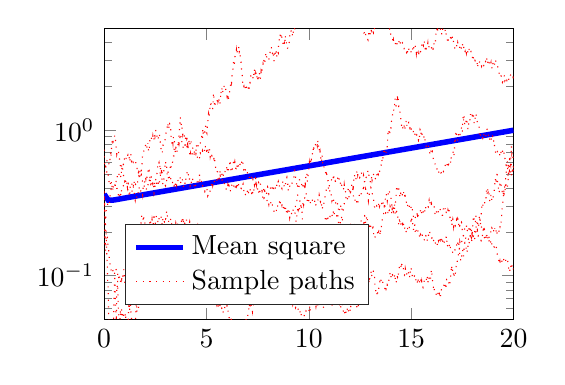
\begin{tikzpicture}

% \begin{axis}[%
% width=5.706cm,
% height=4cm,
% at={(0cm,0cm)},
% scale only axis,
% xmin=0,
% xmax=20,
% ymode=log,
% ymin=0.01,
% ymax=10.4545718358131,
% yminorticks=true,
% axis background/.style={fill=white},
% title style={font=\bfseries},
% title={uncontrolled system},
% legend style={legend cell align=left, align=left, draw=white!15!black}
% ]
\begin{axis}[%
width=5.2cm,
height=3.7cm,
at={(0cm,0cm)},
scale only axis,
xmin=0,
xmax=20,
ymin=0.05,
ymax=5,
ymode=log,
axis background/.style={fill=white},
legend style={at={(0.05,0.05)}, anchor=south west, legend cell align=left, align=left, draw=white!15!black}
]
\addplot [color=blue, line width=2.0pt]
  table[row sep=crcr]{%
0	0.36339119680705\\
0.202020202020202	0.330293084852533\\
0.404040404040404	0.329904816885572\\
0.606060606060606	0.333246911667301\\
0.808080808080808	0.337200739960539\\
1.01010101010101	0.341236643472142\\
1.21212121212121	0.345277509474294\\
1.41414141414141	0.34932495013141\\
1.61616161616162	0.353390119404504\\
1.81818181818182	0.357482324836063\\
2.02020202020202	0.361608183558299\\
2.22222222222222	0.365772309552614\\
2.42424242424242	0.369977972980865\\
2.62626262626263	0.374227558307416\\
2.82828282828283	0.378522864625664\\
3.03030303030303	0.382865301722821\\
3.23232323232323	0.387256019170625\\
3.43434343434343	0.391695992163524\\
3.63636363636364	0.396186079080745\\
3.83838383838384	0.400727060348888\\
4.04040404040404	0.405319664824893\\
4.24242424242424	0.409964587793038\\
4.44444444444444	0.414662503297633\\
4.64646464646465	0.419414072634428\\
4.84848484848485	0.424219950228321\\
5.05050505050505	0.429080787727369\\
5.25252525252525	0.433997236875986\\
5.45454545454545	0.438969951550056\\
5.65656565656566	0.443999589214764\\
5.85858585858586	0.449086811983346\\
6.06060606060606	0.454232287398785\\
6.26262626262626	0.459436689022211\\
6.46464646464646	0.464700696885725\\
6.66666666666667	0.470024997849565\\
6.86868686868687	0.475410285891329\\
7.07070707070707	0.480857262346582\\
7.27272727272727	0.486366636114428\\
7.47474747474747	0.491939123837652\\
7.67676767676768	0.497575450064269\\
7.87878787878788	0.503276347395398\\
8.08080808080808	0.509042556623013\\
8.28282828282828	0.514874826860187\\
8.48484848484848	0.520773915665789\\
8.68686868686869	0.526740589165071\\
8.88888888888889	0.532775622167225\\
9.09090909090909	0.538879798280821\\
9.29292929292929	0.545053910027704\\
9.49494949494949	0.551298758955954\\
9.6969696969697	0.557615155752248\\
9.8989898989899	0.564003920353992\\
10.1010101010101	0.570465882061488\\
10.3030303030303	0.577001879650357\\
10.5050505050505	0.583612761484385\\
10.7070707070707	0.590299385628954\\
10.9090909090909	0.597062619965187\\
11.1111111111111	0.603903342304913\\
11.3131313131313	0.610822440506535\\
11.5151515151515	0.617820812591877\\
11.7171717171717	0.6248993668641\\
11.9191919191919	0.632059022026725\\
12.1212121212121	0.639300707303818\\
12.3232323232323	0.646625362561386\\
12.5252525252525	0.654033938430019\\
12.7272727272727	0.661527396428841\\
12.9292929292929	0.669106709090756\\
13.1313131313131	0.676772860089066\\
13.3333333333333	0.684526844365458\\
13.5353535353535	0.692369668259422\\
13.7373737373737	0.700302349639075\\
13.9393939393939	0.708325918033459\\
14.1414141414141	0.71644141476632\\
14.3434343434343	0.724649893091397\\
14.5454545454545	0.732952418329221\\
14.7474747474747	0.741350068005478\\
14.9494949494949	0.749843931990926\\
15.1515151515152	0.75843511264292\\
15.3535353535354	0.767124724948524\\
15.5555555555556	0.775913896669272\\
15.7575757575758	0.784803768487567\\
15.959595959596	0.793795494154755\\
16.1616161616162	0.8028902406409\\
16.3636363636364	0.812089188286244\\
16.5656565656566	0.821393530954421\\
16.7676767676768	0.830804476187421\\
16.969696969697	0.840323245362319\\
17.1717171717172	0.849951073849794\\
17.3737373737374	0.859689211174474\\
17.5757575757576	0.869538921177112\\
17.7777777777778	0.879501482178615\\
17.979797979798	0.889578187145952\\
18.1818181818182	0.899770343859962\\
18.3838383838384	0.910079275085093\\
18.5858585858586	0.920506318741072\\
18.7878787878788	0.931052828076545\\
18.989898989899	0.941720171844706\\
19.1919191919192	0.952509734480948\\
19.3939393939394	0.963422916282533\\
19.5959595959596	0.974461133590329\\
19.7979797979798	0.985625818972625\\
20	0.996918421411061\\
};
\addlegendentry{Mean square}

\addplot [color=red, dotted]
  table[row sep=crcr]{%
0	0.733104233847529\\
0.02002002002002	0.594520368991298\\
0.04004004004004	0.572160493852255\\
0.0600600600600601	0.54492822137041\\
0.0800800800800801	0.55458131370617\\
0.1001001001001	0.580806954021973\\
0.12012012012012	0.580606760677271\\
0.14014014014014	0.616105538048407\\
0.16016016016016	0.623216277577213\\
0.18018018018018	0.613398477746379\\
0.2002002002002	0.615123104629857\\
0.22022022022022	0.621081916703298\\
0.24024024024024	0.583782487245148\\
0.26026026026026	0.577022480761444\\
0.28028028028028	0.60318658039425\\
0.3003003003003	0.668487637564646\\
0.32032032032032	0.73225659593014\\
0.34034034034034	0.647917860880774\\
0.36036036036036	0.738595735225278\\
0.38038038038038	0.81322243499986\\
0.4004004004004	0.834244414174284\\
0.42042042042042	0.876936320107375\\
0.44044044044044	0.828769207366646\\
0.46046046046046	0.840948836381465\\
0.48048048048048	0.872650726976408\\
0.500500500500501	0.876853676485597\\
0.520520520520521	0.924577733985581\\
0.540540540540541	0.876715830611237\\
0.560560560560561	0.848694103980321\\
0.580580580580581	0.779455587039209\\
0.600600600600601	0.735816694395398\\
0.620620620620621	0.684325993243158\\
0.640640640640641	0.707867895950302\\
0.660660660660661	0.705931419888333\\
0.680680680680681	0.695340238923908\\
0.700700700700701	0.712922946982035\\
0.720720720720721	0.68341128983184\\
0.740740740740741	0.65728463410428\\
0.760760760760761	0.619468169638117\\
0.780780780780781	0.591505087750358\\
0.800800800800801	0.560786634213541\\
0.820820820820821	0.557890444953131\\
0.840840840840841	0.540540760861424\\
0.860860860860861	0.590852775942353\\
0.880880880880881	0.580190626583989\\
0.900900900900901	0.574228534414985\\
0.920920920920921	0.56931901686687\\
0.940940940940941	0.580383281534767\\
0.960960960960961	0.575502650046271\\
0.980980980980981	0.610388859275332\\
1.001001001001	0.654046147573242\\
1.02102102102102	0.655995563722791\\
1.04104104104104	0.660225037825363\\
1.06106106106106	0.666633175962131\\
1.08108108108108	0.630811495532306\\
1.1011011011011	0.62231347711338\\
1.12112112112112	0.639085231235753\\
1.14114114114114	0.661540292431594\\
1.16116116116116	0.671417230272459\\
1.18118118118118	0.638086901184918\\
1.2012012012012	0.625511448168916\\
1.22122122122122	0.632936256059245\\
1.24124124124124	0.657891278687704\\
1.26126126126126	0.614708514766103\\
1.28128128128128	0.645104066184619\\
1.3013013013013	0.685154831192696\\
1.32132132132132	0.666165284464584\\
1.34134134134134	0.611038816185328\\
1.36136136136136	0.618552008354966\\
1.38138138138138	0.587164427107056\\
1.4014014014014	0.6034894554843\\
1.42142142142142	0.600062625082068\\
1.44144144144144	0.623798975912899\\
1.46146146146146	0.610158284697628\\
1.48148148148148	0.609199071019979\\
1.5015015015015	0.603937293784978\\
1.52152152152152	0.602669867426011\\
1.54154154154154	0.605509695346846\\
1.56156156156156	0.58834592533808\\
1.58158158158158	0.556535108069384\\
1.6016016016016	0.558754321891588\\
1.62162162162162	0.532769097903036\\
1.64164164164164	0.52213913738389\\
1.66166166166166	0.503660780449526\\
1.68168168168168	0.511736395678986\\
1.7017017017017	0.468128972249827\\
1.72172172172172	0.483647678186592\\
1.74174174174174	0.492166224338552\\
1.76176176176176	0.504913934607029\\
1.78178178178178	0.506470490426447\\
1.8018018018018	0.488945752051321\\
1.82182182182182	0.493514507238789\\
1.84184184184184	0.46788499392268\\
1.86186186186186	0.455901725115302\\
1.88188188188188	0.438169801416476\\
1.9019019019019	0.429208602490521\\
1.92192192192192	0.426690075849652\\
1.94194194194194	0.42251746177399\\
1.96196196196196	0.431882783544722\\
1.98198198198198	0.442733658774817\\
2.002002002002	0.462584580665438\\
2.02202202202202	0.476816506922267\\
2.04204204204204	0.461805492164541\\
2.06206206206206	0.482370406191094\\
2.08208208208208	0.465887170057703\\
2.1021021021021	0.476398889299475\\
2.12212212212212	0.477248857401529\\
2.14214214214214	0.507023203412549\\
2.16216216216216	0.548546187585548\\
2.18218218218218	0.525987339499815\\
2.2022022022022	0.528070228348133\\
2.22222222222222	0.502216769724132\\
2.24224224224224	0.470622448257631\\
2.26226226226226	0.435877619015479\\
2.28228228228228	0.424562130962317\\
2.3023023023023	0.428576370025505\\
2.32232232232232	0.422289440316076\\
2.34234234234234	0.436422296757815\\
2.36236236236236	0.43942424540502\\
2.38238238238238	0.426906809677588\\
2.4024024024024	0.434572826240591\\
2.42242242242242	0.422234308774215\\
2.44244244244244	0.432616829805794\\
2.46246246246246	0.438441672180264\\
2.48248248248248	0.419447984478959\\
2.5025025025025	0.435977203696887\\
2.52252252252252	0.432614252671657\\
2.54254254254254	0.435865072967486\\
2.56256256256256	0.436795078822685\\
2.58258258258258	0.418666228895894\\
2.6026026026026	0.425340999650149\\
2.62262262262262	0.435008588223772\\
2.64264264264264	0.42606085030444\\
2.66266266266266	0.454768445803023\\
2.68268268268268	0.445925523496646\\
2.7027027027027	0.436851386820005\\
2.72272272272272	0.457014200760422\\
2.74274274274274	0.48078354576739\\
2.76276276276276	0.499252443216527\\
2.78278278278278	0.497422523032156\\
2.8028028028028	0.486325490354298\\
2.82282282282282	0.46444644788965\\
2.84284284284284	0.445368560252808\\
2.86286286286286	0.422244868958616\\
2.88288288288288	0.447966622672134\\
2.9029029029029	0.468344096910546\\
2.92292292292292	0.461012833285025\\
2.94294294294294	0.441723552462682\\
2.96296296296296	0.438327393644266\\
2.98298298298298	0.420445138858625\\
3.003003003003	0.414940196750389\\
3.02302302302302	0.433475550574024\\
3.04304304304304	0.430098487988357\\
3.06306306306306	0.458198349255386\\
3.08308308308308	0.461456500896196\\
3.1031031031031	0.478426600866451\\
3.12312312312312	0.483723774185741\\
3.14314314314314	0.469459099882564\\
3.16316316316316	0.448426341033864\\
3.18318318318318	0.460605351462094\\
3.2032032032032	0.480126172724692\\
3.22322322322322	0.451330523839044\\
3.24324324324324	0.456658163871632\\
3.26326326326326	0.467604030357473\\
3.28328328328328	0.471172489447954\\
3.3033033033033	0.456946749539117\\
3.32332332332332	0.437480343583111\\
3.34334334334334	0.437532995291557\\
3.36336336336336	0.419299419858948\\
3.38338338338338	0.402977573530326\\
3.4034034034034	0.407554657105689\\
3.42342342342342	0.413651857299992\\
3.44344344344344	0.405189255117621\\
3.46346346346346	0.418577226391484\\
3.48348348348348	0.431438480190671\\
3.5035035035035	0.4146392424961\\
3.52352352352352	0.433866535864208\\
3.54354354354354	0.419436463131331\\
3.56356356356356	0.44048974459666\\
3.58358358358358	0.438723082645756\\
3.6036036036036	0.455056361650415\\
3.62362362362362	0.442953780781874\\
3.64364364364364	0.447208652909173\\
3.66366366366366	0.442805178587103\\
3.68368368368368	0.457459731236141\\
3.7037037037037	0.45770940345666\\
3.72372372372372	0.477345205565243\\
3.74374374374374	0.436158223125418\\
3.76376376376376	0.434549821709767\\
3.78378378378378	0.444887290221705\\
3.8038038038038	0.465716310265458\\
3.82382382382382	0.459338951780872\\
3.84384384384384	0.435415802343556\\
3.86386386386386	0.432539115073784\\
3.88388388388388	0.403704333702725\\
3.9039039039039	0.410263066520516\\
3.92392392392392	0.40710752438454\\
3.94394394394394	0.411863783300981\\
3.96396396396396	0.459769249373987\\
3.98398398398398	0.450643930454831\\
4.004004004004	0.465038288341573\\
4.02402402402402	0.48929801629607\\
4.04404404404404	0.503205502045644\\
4.06406406406406	0.518376827179955\\
4.08408408408408	0.517625137567342\\
4.1041041041041	0.485696788665042\\
4.12412412412412	0.497390290370127\\
4.14414414414414	0.502173775672092\\
4.16416416416416	0.478858164816956\\
4.18418418418418	0.440208193178229\\
4.2042042042042	0.416221144794781\\
4.22422422422422	0.428134768229551\\
4.24424424424424	0.416525124627036\\
4.26426426426426	0.438752067390839\\
4.28428428428428	0.438742410289285\\
4.3043043043043	0.469834664088193\\
4.32432432432432	0.461369816473394\\
4.34434434434434	0.441205690248672\\
4.36436436436436	0.436094391988541\\
4.38438438438438	0.429720805915175\\
4.4044044044044	0.404289989400132\\
4.42442442442442	0.395118359331945\\
4.44444444444444	0.396186941439534\\
4.46446446446446	0.408955968892174\\
4.48448448448448	0.426891269932629\\
4.5045045045045	0.435918595951579\\
4.52452452452452	0.437894507616889\\
4.54454454454454	0.450087319764461\\
4.56456456456456	0.427858050877779\\
4.58458458458458	0.419127303604961\\
4.6046046046046	0.428416985100365\\
4.62462462462462	0.437213876272126\\
4.64464464464464	0.44478377082696\\
4.66466466466466	0.496965647301747\\
4.68468468468468	0.447853044514018\\
4.7047047047047	0.431700671202695\\
4.72472472472472	0.430874975296929\\
4.74474474474474	0.44716151609396\\
4.76476476476476	0.439720557199192\\
4.78478478478478	0.411792383345006\\
4.8048048048048	0.419543863880281\\
4.82482482482482	0.412591390915347\\
4.84484484484484	0.414616655769985\\
4.86486486486486	0.402881788743906\\
4.88488488488488	0.401851262505983\\
4.9049049049049	0.390088116585959\\
4.92492492492492	0.378458600408418\\
4.94494494494494	0.383199585719096\\
4.96496496496496	0.385992312532224\\
4.98498498498498	0.39904481669021\\
5.00500500500501	0.397030536136155\\
5.02502502502503	0.398681277683926\\
5.04504504504505	0.373195623862782\\
5.06506506506507	0.353437062732699\\
5.08508508508509	0.358826533348017\\
5.10510510510511	0.361637089996692\\
5.12512512512513	0.376596715527055\\
5.14514514514515	0.370979311766325\\
5.16516516516517	0.375470038563129\\
5.18518518518519	0.385357465472814\\
5.20520520520521	0.396948760432401\\
5.22522522522523	0.404894646737707\\
5.24524524524525	0.416712702453355\\
5.26526526526527	0.439717638834218\\
5.28528528528529	0.433287710231502\\
5.30530530530531	0.416860427501071\\
5.32532532532533	0.434185120791048\\
5.34534534534535	0.443844349673764\\
5.36536536536537	0.433640145911698\\
5.38538538538539	0.441732078191532\\
5.40540540540541	0.450332145524977\\
5.42542542542543	0.454474686893093\\
5.44544544544545	0.448864173295384\\
5.46546546546547	0.449694267327818\\
5.48548548548549	0.458613858217384\\
5.50550550550551	0.463625382452616\\
5.52552552552553	0.433532740521229\\
5.54554554554555	0.448004125610234\\
5.56556556556557	0.482800664541345\\
5.58558558558559	0.465679082193324\\
5.60560560560561	0.47032791508113\\
5.62562562562563	0.465873835527599\\
5.64564564564565	0.485415928832782\\
5.66566566566567	0.525611185835319\\
5.68568568568569	0.476947851307544\\
5.70570570570571	0.506383309676565\\
5.72572572572573	0.500936627933458\\
5.74574574574575	0.502697120010266\\
5.76576576576577	0.4887779866416\\
5.78578578578579	0.474565393190053\\
5.80580580580581	0.468589814786965\\
5.82582582582583	0.490607466372949\\
5.84584584584585	0.504954114404337\\
5.86586586586587	0.523815615960296\\
5.88588588588589	0.519218951374336\\
5.90590590590591	0.512613790768152\\
5.92592592592593	0.535148823185457\\
5.94594594594595	0.537970530488121\\
5.96596596596597	0.54613160739336\\
5.98598598598599	0.561540140134908\\
6.00600600600601	0.514841633282101\\
6.02602602602603	0.543490143347283\\
6.04604604604605	0.553884651912483\\
6.06606606606607	0.525907861488995\\
6.08608608608609	0.547031982998238\\
6.10610610610611	0.549565482100832\\
6.12612612612613	0.55125404453479\\
6.14614614614615	0.622949976812883\\
6.16616616616617	0.597410623974369\\
6.18618618618619	0.545497379640962\\
6.20620620620621	0.525295093374531\\
6.22622622622623	0.513040640307268\\
6.24624624624625	0.511603245917049\\
6.26626626626627	0.547107852658371\\
6.28628628628629	0.574566050595935\\
6.30630630630631	0.577918635009642\\
6.32632632632633	0.631218801103005\\
6.34634634634635	0.568645877251789\\
6.36636636636637	0.580406822084783\\
6.38638638638639	0.601969359187513\\
6.40640640640641	0.569749008928537\\
6.42642642642643	0.547117784463605\\
6.44644644644645	0.544655087283765\\
6.46646646646647	0.577207667883845\\
6.48648648648649	0.581843973249576\\
6.50650650650651	0.548692548244684\\
6.52652652652653	0.578339928533954\\
6.54654654654655	0.575693042376063\\
6.56656656656657	0.562427870524777\\
6.58658658658659	0.546280984820784\\
6.60660660660661	0.560723353164044\\
6.62662662662663	0.57983745353785\\
6.64664664664665	0.581614043154479\\
6.66666666666667	0.58004405429755\\
6.68668668668669	0.570927729492821\\
6.70670670670671	0.563531377856848\\
6.72672672672673	0.62028364064424\\
6.74674674674675	0.627826496283051\\
6.76676676676677	0.617952459881571\\
6.78678678678679	0.587839771523889\\
6.80680680680681	0.553130220879507\\
6.82682682682683	0.533995302496369\\
6.84684684684685	0.53728082761899\\
6.86686686686687	0.529258969375295\\
6.88688688688689	0.552467706790798\\
6.90690690690691	0.532150027449003\\
6.92692692692693	0.525753535003781\\
6.94694694694695	0.540050726415918\\
6.96696696696697	0.534162144820446\\
6.98698698698699	0.520758702589756\\
7.00700700700701	0.502255582758982\\
7.02702702702703	0.502388996544338\\
7.04704704704705	0.507956043700771\\
7.06706706706707	0.490865257292919\\
7.08708708708709	0.479264077959796\\
7.10710710710711	0.460459252346955\\
7.12712712712713	0.475013066025893\\
7.14714714714715	0.471822030201924\\
7.16716716716717	0.470721385725451\\
7.18718718718719	0.465757451304294\\
7.20720720720721	0.478481020510526\\
7.22722722722723	0.457522734637947\\
7.24724724724725	0.449166663249813\\
7.26726726726727	0.458843595125608\\
7.28728728728729	0.442949791751309\\
7.30730730730731	0.448734865303105\\
7.32732732732733	0.435901163051546\\
7.34734734734735	0.420669614701535\\
7.36736736736737	0.438961282237757\\
7.38738738738739	0.445355697175844\\
7.40740740740741	0.466934793954488\\
7.42742742742743	0.461902456419519\\
7.44744744744745	0.420417194155098\\
7.46746746746747	0.432366353141407\\
7.48748748748749	0.436553811062648\\
7.50750750750751	0.425360245512985\\
7.52752752752753	0.429159662454684\\
7.54754754754755	0.435644431602106\\
7.56756756756757	0.426157025839157\\
7.58758758758759	0.41553440334914\\
7.60760760760761	0.415270740107034\\
7.62762762762763	0.430845258290592\\
7.64764764764765	0.418963358864412\\
7.66766766766767	0.417691229853436\\
7.68768768768769	0.403271675685746\\
7.70770770770771	0.391968299644005\\
7.72772772772773	0.367039906056319\\
7.74774774774775	0.345574488729965\\
7.76776776776777	0.332757047439598\\
7.78778778778779	0.345958430840858\\
7.80780780780781	0.340500073308182\\
7.82782782782783	0.343171425711825\\
7.84784784784785	0.344626420507017\\
7.86786786786787	0.336701198396834\\
7.88788788788789	0.338576867628415\\
7.90790790790791	0.332150244053992\\
7.92792792792793	0.336340669067314\\
7.94794794794795	0.333213237835585\\
7.96796796796797	0.325276733563507\\
7.98798798798799	0.318952679288842\\
8.00800800800801	0.311332439055359\\
8.02802802802803	0.318418519736371\\
8.04804804804805	0.309204052081565\\
8.06806806806807	0.322411857514077\\
8.08808808808809	0.31434845209135\\
8.10810810810811	0.311660254889777\\
8.12812812812813	0.312658495454317\\
8.14814814814815	0.318347211783745\\
8.16816816816817	0.325339692007207\\
8.18818818818819	0.327373143136306\\
8.20820820820821	0.321096420291748\\
8.22822822822823	0.295930443001947\\
8.24824824824825	0.286111168805266\\
8.26826826826827	0.284175879555473\\
8.28828828828829	0.278173288382026\\
8.30830830830831	0.277398206631688\\
8.32832832832833	0.275466817448866\\
8.34834834834835	0.278870456117912\\
8.36836836836837	0.279250480351156\\
8.38838838838839	0.281967504765511\\
8.40840840840841	0.272859491645505\\
8.42842842842843	0.293945657977085\\
8.44844844844845	0.296201307244413\\
8.46846846846847	0.291511168263717\\
8.48848848848849	0.309682603304439\\
8.50850850850851	0.316686886121467\\
8.52852852852853	0.31554111417825\\
8.54854854854855	0.324899932680649\\
8.56856856856857	0.322107281514936\\
8.58858858858859	0.302802485028739\\
8.60860860860861	0.31804278759978\\
8.62862862862863	0.326422154787873\\
8.64864864864865	0.327774109056395\\
8.66866866866867	0.316817811321561\\
8.68868868868869	0.305508816289726\\
8.70870870870871	0.314652076559789\\
8.72872872872873	0.308567346792438\\
8.74874874874875	0.299668567545032\\
8.76876876876877	0.285306499053833\\
8.78878878878879	0.299120168312679\\
8.80880880880881	0.292513233597987\\
8.82882882882883	0.284895018092446\\
8.84884884884885	0.275685180716426\\
8.86886886886887	0.290013210720153\\
8.88888888888889	0.297503447502535\\
8.90890890890891	0.272727936912877\\
8.92892892892893	0.286081873077024\\
8.94894894894895	0.279654505455777\\
8.96896896896897	0.261953837471874\\
8.98898898898899	0.282854771729021\\
9.00900900900901	0.278043186808956\\
9.02902902902903	0.2874099670075\\
9.04904904904905	0.269396216484061\\
9.06906906906907	0.251002021938167\\
9.08908908908909	0.260576645048612\\
9.10910910910911	0.259857876768732\\
9.12912912912913	0.255360256012885\\
9.14914914914915	0.257593280339441\\
9.16916916916917	0.280506489963474\\
9.18918918918919	0.287093422849957\\
9.20920920920921	0.288260336297487\\
9.22922922922923	0.284616616228802\\
9.24924924924925	0.272779953034664\\
9.26926926926927	0.26630814989911\\
9.28928928928929	0.262129765707224\\
9.30930930930931	0.267693897992146\\
9.32932932932933	0.268714141911863\\
9.34934934934935	0.305284584394184\\
9.36936936936937	0.307827951812889\\
9.38938938938939	0.307795292409453\\
9.40940940940941	0.309941259060366\\
9.42942942942943	0.349919786741511\\
9.44944944944945	0.36101784736152\\
9.46946946946947	0.353013487317128\\
9.48948948948949	0.352866932630835\\
9.50950950950951	0.3477775767713\\
9.52952952952953	0.338287217825808\\
9.54954954954955	0.330769470954243\\
9.56956956956957	0.324528841231502\\
9.58958958958959	0.322966822624663\\
9.60960960960961	0.32125538960644\\
9.62962962962963	0.299872988353528\\
9.64964964964965	0.29087135267928\\
9.66966966966967	0.292478774067498\\
9.68968968968969	0.290590071452982\\
9.70970970970971	0.312392794163032\\
9.72972972972973	0.326310471154353\\
9.74974974974975	0.307678405783581\\
9.76976976976977	0.319249039190596\\
9.78978978978979	0.325465552162845\\
9.80980980980981	0.357415708276135\\
9.82982982982983	0.365071450731154\\
9.84984984984985	0.369506284496934\\
9.86986986986987	0.370631672218541\\
9.88988988988989	0.350317026040488\\
9.90990990990991	0.346986893299141\\
9.92992992992993	0.322386041372451\\
9.94994994994995	0.337178653158223\\
9.96996996996997	0.337381045859746\\
9.98998998998999	0.33543883627308\\
10.01001001001	0.320326314567396\\
10.03003003003	0.311475445794133\\
10.0500500500501	0.321160830441247\\
10.0700700700701	0.322382524718419\\
10.0900900900901	0.310214049220142\\
10.1101101101101	0.323438621615929\\
10.1301301301301	0.323726014442677\\
10.1501501501502	0.322500821271125\\
10.1701701701702	0.327503452537959\\
10.1901901901902	0.336370901574986\\
10.2102102102102	0.333663430247469\\
10.2302302302302	0.334868467107592\\
10.2502502502503	0.340246421454195\\
10.2702702702703	0.337505897061231\\
10.2902902902903	0.32247614097631\\
10.3103103103103	0.311517667969554\\
10.3303303303303	0.319346018416176\\
10.3503503503504	0.305411535581277\\
10.3703703703704	0.304727357130746\\
10.3903903903904	0.305275516485179\\
10.4104104104104	0.31151945544896\\
10.4304304304304	0.319893008342255\\
10.4504504504505	0.337622406400278\\
10.4704704704705	0.33292228990227\\
10.4904904904905	0.332648486753966\\
10.5105105105105	0.356917825947466\\
10.5305305305305	0.347744978586736\\
10.5505505505506	0.33082528766302\\
10.5705705705706	0.322639869878\\
10.5905905905906	0.330146757419656\\
10.6106106106106	0.323277162731726\\
10.6306306306306	0.29965253736409\\
10.6506506506507	0.308619310267122\\
10.6706706706707	0.291036365069702\\
10.6906906906907	0.288129440744297\\
10.7107107107107	0.301003918917833\\
10.7307307307307	0.30728338879992\\
10.7507507507508	0.323964771221288\\
10.7707707707708	0.334266440299956\\
10.7907907907908	0.34448677380145\\
10.8108108108108	0.363603072290404\\
10.8308308308308	0.374022931884967\\
10.8508508508509	0.385874535188142\\
10.8708708708709	0.400622118900265\\
10.8908908908909	0.40048742896999\\
10.9109109109109	0.398239395070094\\
10.9309309309309	0.400959549257814\\
10.950950950951	0.392142040609432\\
10.970970970971	0.408714067074387\\
10.990990990991	0.410842259228692\\
11.011011011011	0.394953156242788\\
11.031031031031	0.379208781310313\\
11.0510510510511	0.360171509104618\\
11.0710710710711	0.367694601804972\\
11.0910910910911	0.361389659934823\\
11.1111111111111	0.342916936179103\\
11.1311311311311	0.325427618754981\\
11.1511511511512	0.332057844902045\\
11.1711711711712	0.337519084045751\\
11.1911911911912	0.321977222161848\\
11.2112112112112	0.329011152358694\\
11.2312312312312	0.335105436140427\\
11.2512512512513	0.335117633531155\\
11.2712712712713	0.338374203738486\\
11.2912912912913	0.333997986539837\\
11.3113113113113	0.315254256543028\\
11.3313313313313	0.310083837015236\\
11.3513513513514	0.299229885333002\\
11.3713713713714	0.299517626608902\\
11.3913913913914	0.307851221127137\\
11.4114114114114	0.314698701153584\\
11.4314314314314	0.301824085031328\\
11.4514514514515	0.278604445826718\\
11.4714714714715	0.280531056374738\\
11.4914914914915	0.291987179689184\\
11.5115115115115	0.277327638990981\\
11.5315315315315	0.289084921095098\\
11.5515515515516	0.293312673397432\\
11.5715715715716	0.30828897885884\\
11.5915915915916	0.306719750405012\\
11.6116116116116	0.29671252145078\\
11.6316316316316	0.275446374777876\\
11.6516516516517	0.270428907010354\\
11.6716716716717	0.274063098358448\\
11.6916916916917	0.289148186270047\\
11.7117117117117	0.309065449345253\\
11.7317317317317	0.310747163437254\\
11.7517517517518	0.337539225782477\\
11.7717717717718	0.339071488053657\\
11.7917917917918	0.342267647197662\\
11.8118118118118	0.342940139356997\\
11.8318318318318	0.355026360212576\\
11.8518518518519	0.343954699821278\\
11.8718718718719	0.334683403469213\\
11.8918918918919	0.338378315569602\\
11.9119119119119	0.342309477160182\\
11.9319319319319	0.335765431828934\\
11.951951951952	0.354200092165538\\
11.971971971972	0.345887318945109\\
11.991991991992	0.341493612515229\\
12.012012012012	0.349157575595777\\
12.032032032032	0.370928276942724\\
12.0520520520521	0.367348522522696\\
12.0720720720721	0.3647752399668\\
12.0920920920921	0.372248999754818\\
12.1121121121121	0.371019555163595\\
12.1321321321321	0.381486186472598\\
12.1521521521522	0.391633225578925\\
12.1721721721722	0.36110979713638\\
12.1921921921922	0.340734572286031\\
12.2122122122122	0.336253961823847\\
12.2322322322322	0.337347000248945\\
12.2522522522523	0.326218630079511\\
12.2722722722723	0.340744901887254\\
12.2922922922923	0.33493543165527\\
12.3123123123123	0.320648951847385\\
12.3323323323323	0.320809123636253\\
12.3523523523524	0.327710681421862\\
12.3723723723724	0.317840737155604\\
12.3923923923924	0.311058880942105\\
12.4124124124124	0.324192009057548\\
12.4324324324324	0.342042220628513\\
12.4524524524525	0.344767308314665\\
12.4724724724725	0.361345940550899\\
12.4924924924925	0.350486825798126\\
12.5125125125125	0.364995212894403\\
12.5325325325325	0.363320502368042\\
12.5525525525526	0.364537736685767\\
12.5725725725726	0.367302006918401\\
12.5925925925926	0.374560967742439\\
12.6126126126126	0.377668177347988\\
12.6326326326326	0.382254140627116\\
12.6526526526527	0.380100271209826\\
12.6726726726727	0.42177677213795\\
12.6926926926927	0.392207104605275\\
12.7127127127127	0.383317850708622\\
12.7327327327327	0.383855278633706\\
12.7527527527528	0.38182314944006\\
12.7727727727728	0.394019653123716\\
12.7927927927928	0.382767797130746\\
12.8128128128128	0.388891632115426\\
12.8328328328328	0.386766390326153\\
12.8528528528529	0.386545084901027\\
12.8728728728729	0.36087591994742\\
12.8928928928929	0.352763023263933\\
12.9129129129129	0.329197594202661\\
12.9329329329329	0.348967303560839\\
12.952952952953	0.360776729808502\\
12.972972972973	0.376493637150615\\
12.992992992993	0.384883921019557\\
13.013013013013	0.388883477036761\\
13.033033033033	0.40209433260992\\
13.0530530530531	0.396359224979488\\
13.0730730730731	0.39412804284087\\
13.0930930930931	0.371595130546898\\
13.1131131131131	0.358045933801813\\
13.1331331331331	0.351049378563476\\
13.1531531531532	0.343376450170218\\
13.1731731731732	0.325996661937261\\
13.1931931931932	0.312784490706851\\
13.2132132132132	0.296930890554683\\
13.2332332332332	0.290552263738203\\
13.2532532532533	0.301981279430362\\
13.2732732732733	0.305448791388864\\
13.2932932932933	0.300559744459283\\
13.3133133133133	0.302150873161636\\
13.3333333333333	0.292252924832546\\
13.3533533533534	0.291228458270921\\
13.3733733733734	0.290451774445031\\
13.3933933933934	0.294105672956535\\
13.4134134134134	0.309786290203759\\
13.4334334334334	0.318932402255998\\
13.4534534534535	0.29932256018241\\
13.4734734734735	0.305667761054564\\
13.4934934934935	0.300176186062982\\
13.5135135135135	0.310086039832253\\
13.5335335335335	0.316626419143447\\
13.5535535535536	0.314363249798995\\
13.5735735735736	0.312069129749783\\
13.5935935935936	0.311012895266532\\
13.6136136136136	0.327894773282761\\
13.6336336336336	0.307675282350517\\
13.6536536536537	0.312043397745694\\
13.6736736736737	0.297505804764227\\
13.6936936936937	0.302588890759241\\
13.7137137137137	0.31715581488307\\
13.7337337337337	0.328663895714549\\
13.7537537537538	0.359810507945484\\
13.7737737737738	0.365672815649598\\
13.7937937937938	0.359223139575697\\
13.8138138138138	0.34627999372188\\
13.8338338338338	0.326357443984739\\
13.8538538538539	0.340341070365195\\
13.8738738738739	0.361065084456885\\
13.8938938938939	0.373431937242641\\
13.9139139139139	0.365179493711156\\
13.9339339339339	0.380992566139612\\
13.953953953954	0.37028244813181\\
13.973973973974	0.36494279540723\\
13.993993993994	0.350993248250887\\
14.014014014014	0.34405229068448\\
14.034034034034	0.317953038145534\\
14.0540540540541	0.306893659266018\\
14.0740740740741	0.295979075437936\\
14.0940940940941	0.298706450585654\\
14.1141141141141	0.28561004825345\\
14.1341341341341	0.306473901583904\\
14.1541541541542	0.283411166293083\\
14.1741741741742	0.289459368115618\\
14.1941941941942	0.309712486277803\\
14.2142142142142	0.324606012912845\\
14.2342342342342	0.31581868451625\\
14.2542542542543	0.33688808966766\\
14.2742742742743	0.369558520326193\\
14.2942942942943	0.410390188462349\\
14.3143143143143	0.395821917430983\\
14.3343343343343	0.389237051231354\\
14.3543543543544	0.396373047096928\\
14.3743743743744	0.414612704427666\\
14.3943943943944	0.398004608681712\\
14.4144144144144	0.372975520416834\\
14.4344344344344	0.366101252008089\\
14.4544544544545	0.342833030520285\\
14.4744744744745	0.358039854586352\\
14.4944944944945	0.368925699526959\\
14.5145145145145	0.367555890084516\\
14.5345345345345	0.366894063462613\\
14.5545545545546	0.378971422493311\\
14.5745745745746	0.351132618376916\\
14.5945945945946	0.352687972087459\\
14.6146146146146	0.349444385872626\\
14.6346346346346	0.375898333958527\\
14.6546546546547	0.361053633592255\\
14.6746746746747	0.367189353810946\\
14.6946946946947	0.335442651574425\\
14.7147147147147	0.353115327617089\\
14.7347347347347	0.350455234286253\\
14.7547547547548	0.326822469832688\\
14.7747747747748	0.315367369688656\\
14.7947947947948	0.307027847952281\\
14.8148148148148	0.295689151396731\\
14.8348348348348	0.306985242617064\\
14.8548548548549	0.301207961930223\\
14.8748748748749	0.291712726023529\\
14.8948948948949	0.290188356270363\\
14.9149149149149	0.300410190749174\\
14.9349349349349	0.311947031844161\\
14.954954954955	0.309823461850839\\
14.974974974975	0.308783125195395\\
14.994994994995	0.290842123212647\\
15.015015015015	0.277343552408228\\
15.035035035035	0.283832645345696\\
15.0550550550551	0.286178232506946\\
15.0750750750751	0.27393662071397\\
15.0950950950951	0.264864325839368\\
15.1151151151151	0.250407265500147\\
15.1351351351351	0.255054484178798\\
15.1551551551552	0.25727986697672\\
15.1751751751752	0.256426145946861\\
15.1951951951952	0.248184807482059\\
15.2152152152152	0.255939431028933\\
15.2352352352352	0.264658159264439\\
15.2552552552553	0.270293742687832\\
15.2752752752753	0.271618574349421\\
15.2952952952953	0.264364786060845\\
15.3153153153153	0.274351589009376\\
15.3353353353353	0.258516481195308\\
15.3553553553554	0.261455708087378\\
15.3753753753754	0.258776040815252\\
15.3953953953954	0.260080422146517\\
15.4154154154154	0.26232265467472\\
15.4354354354354	0.267220438075272\\
15.4554554554555	0.279358712340268\\
15.4754754754755	0.28978017161979\\
15.4954954954955	0.278141589808489\\
15.5155155155155	0.267669422019002\\
15.5355355355355	0.26506761851153\\
15.5555555555556	0.25939034849893\\
15.5755755755756	0.271418689527759\\
15.5955955955956	0.276926388323638\\
15.6156156156156	0.282043846894959\\
15.6356356356356	0.290242744513859\\
15.6556556556557	0.289511910183861\\
15.6756756756757	0.271203173368028\\
15.6956956956957	0.285908173879531\\
15.7157157157157	0.296830830151312\\
15.7357357357357	0.296336493667006\\
15.7557557557558	0.300685171588692\\
15.7757757757758	0.303297728720124\\
15.7957957957958	0.308552941758619\\
15.8158158158158	0.299451631000476\\
15.8358358358358	0.297080558506759\\
15.8558558558559	0.318428938013762\\
15.8758758758759	0.328585609476029\\
15.8958958958959	0.313399988167323\\
15.9159159159159	0.324680938385414\\
15.9359359359359	0.309486125884072\\
15.955955955956	0.297226316762948\\
15.975975975976	0.302922544730234\\
15.995995995996	0.311405313808085\\
16.016016016016	0.300646433096369\\
16.036036036036	0.302294378546711\\
16.0560560560561	0.304426604586936\\
16.0760760760761	0.298531410345818\\
16.0960960960961	0.29967670124113\\
16.1161161161161	0.298437181604704\\
16.1361361361361	0.293939321695648\\
16.1561561561562	0.26939443158257\\
16.1761761761762	0.264692461702636\\
16.1961961961962	0.268687155838915\\
16.2162162162162	0.282057919089321\\
16.2362362362362	0.274185123609806\\
16.2562562562563	0.270789660389498\\
16.2762762762763	0.263318482414814\\
16.2962962962963	0.273302341241256\\
16.3163163163163	0.271079368001377\\
16.3363363363363	0.282433117990299\\
16.3563563563564	0.282741077609641\\
16.3763763763764	0.292723957965924\\
16.3963963963964	0.292357843490249\\
16.4164164164164	0.286180097459872\\
16.4364364364364	0.279708215979984\\
16.4564564564565	0.267377406912973\\
16.4764764764765	0.267734432804676\\
16.4964964964965	0.263650674857031\\
16.5165165165165	0.259986620670377\\
16.5365365365365	0.260001543157091\\
16.5565565565566	0.272069372267688\\
16.5765765765766	0.292586034211649\\
16.5965965965966	0.290763157033548\\
16.6166166166166	0.286347267611897\\
16.6366366366366	0.296319716936929\\
16.6566566566567	0.291235784821483\\
16.6766766766767	0.274687407793982\\
16.6966966966967	0.28135550257106\\
16.7167167167167	0.271729259954783\\
16.7367367367367	0.271851829326902\\
16.7567567567568	0.265837791085541\\
16.7767767767768	0.273068167958535\\
16.7967967967968	0.282547248138836\\
16.8168168168168	0.275356618437691\\
16.8368368368368	0.289531889497837\\
16.8568568568569	0.279167171781501\\
16.8768768768769	0.266563503995068\\
16.8968968968969	0.251675756469072\\
16.9169169169169	0.252410734785259\\
16.9369369369369	0.253926508362442\\
16.956956956957	0.235784893201268\\
16.976976976977	0.244643432149135\\
16.996996996997	0.22223371316119\\
17.017017017017	0.233304830655961\\
17.037037037037	0.243312039968715\\
17.0570570570571	0.235941555441106\\
17.0770770770771	0.218465163816154\\
17.0970970970971	0.230480676782683\\
17.1171171171171	0.226679581339321\\
17.1371371371371	0.224898935870864\\
17.1571571571572	0.220011606902455\\
17.1771771771772	0.222952881453748\\
17.1971971971972	0.235499801264952\\
17.2172172172172	0.241362235071968\\
17.2372372372372	0.232074738980347\\
17.2572572572573	0.232358809798276\\
17.2772772772773	0.245930998744919\\
17.2972972972973	0.241881169728053\\
17.3173173173173	0.222624541941875\\
17.3373373373373	0.234289658277086\\
17.3573573573574	0.231442551954469\\
17.3773773773774	0.218531970762326\\
17.3973973973974	0.219087425860096\\
17.4174174174174	0.229230830873093\\
17.4374374374374	0.22678179492367\\
17.4574574574575	0.232259858547575\\
17.4774774774775	0.22880497786896\\
17.4974974974975	0.20706066425874\\
17.5175175175175	0.206325143206634\\
17.5375375375375	0.198199713087106\\
17.5575575575576	0.186764434754271\\
17.5775775775776	0.179219060501682\\
17.5975975975976	0.183235223884236\\
17.6176176176176	0.183081362698532\\
17.6376376376376	0.180319100583307\\
17.6576576576577	0.180993499441185\\
17.6776776776777	0.18118438072539\\
17.6976976976977	0.180666107580657\\
17.7177177177177	0.179969466232792\\
17.7377377377377	0.183233756794689\\
17.7577577577578	0.183416428703747\\
17.7777777777778	0.175688284621296\\
17.7977977977978	0.17836114421581\\
17.8178178178178	0.179602826011755\\
17.8378378378378	0.182084866208079\\
17.8578578578579	0.184304639184203\\
17.8778778778779	0.189740789996225\\
17.8978978978979	0.188476961402884\\
17.9179179179179	0.187050514597173\\
17.9379379379379	0.183274354634735\\
17.957957957958	0.196941052903783\\
17.977977977978	0.191288700135476\\
17.997997997998	0.199064695844828\\
18.018018018018	0.188746244816563\\
18.038038038038	0.187104929433821\\
18.0580580580581	0.191294821984799\\
18.0780780780781	0.193169572685756\\
18.0980980980981	0.203956448887321\\
18.1181181181181	0.197771593958962\\
18.1381381381381	0.201841123632773\\
18.1581581581582	0.20683833098255\\
18.1781781781782	0.21703999194389\\
18.1981981981982	0.221229678344127\\
18.2182182182182	0.228050195285637\\
18.2382382382382	0.222790414424423\\
18.2582582582583	0.230777236156401\\
18.2782782782783	0.237045929376648\\
18.2982982982983	0.23891269229676\\
18.3183183183183	0.24069965368708\\
18.3383383383383	0.261362814652532\\
18.3583583583584	0.234477793736403\\
18.3783783783784	0.224142448145759\\
18.3983983983984	0.233673951945136\\
18.4184184184184	0.224189449638904\\
18.4384384384384	0.213593674436486\\
18.4584584584585	0.208385693005175\\
18.4784784784785	0.210697970703694\\
18.4984984984985	0.202970162397521\\
18.5185185185185	0.206199996657269\\
18.5385385385385	0.196421685511609\\
18.5585585585586	0.202200216892959\\
18.5785785785786	0.207556987482631\\
18.5985985985986	0.204087569614186\\
18.6186186186186	0.198770183575807\\
18.6386386386386	0.194889346761272\\
18.6586586586587	0.190937649389177\\
18.6786786786787	0.188893969579729\\
18.6986986986987	0.188756737821177\\
18.7187187187187	0.187682302576538\\
18.7387387387387	0.185118671481754\\
18.7587587587588	0.188873473829879\\
18.7787787787788	0.186452592632376\\
18.7987987987988	0.180989858934813\\
18.8188188188188	0.187761497395447\\
18.8388388388388	0.186975446967197\\
18.8588588588589	0.187904324130133\\
18.8788788788789	0.189142914817142\\
18.8988988988989	0.206821799596288\\
18.9189189189189	0.203235672413689\\
18.9389389389389	0.212901714663308\\
18.958958958959	0.210906110812551\\
18.978978978979	0.208107189738713\\
18.998998998999	0.209479210388271\\
19.019019019019	0.214457341164666\\
19.039039039039	0.197449464728228\\
19.0590590590591	0.199919841186338\\
19.0790790790791	0.212110350590108\\
19.0990990990991	0.197527574546841\\
19.1191191191191	0.198940404361121\\
19.1391391391391	0.200132748292123\\
19.1591591591592	0.208082893508292\\
19.1791791791792	0.21025539620525\\
19.1991991991992	0.195656057040969\\
19.2192192192192	0.193085575556611\\
19.2392392392392	0.191701261366359\\
19.2592592592593	0.199265007269555\\
19.2792792792793	0.197187157150919\\
19.2992992992993	0.207301328337383\\
19.3193193193193	0.220449689415655\\
19.3393393393393	0.216775368813828\\
19.3593593593594	0.221908888495403\\
19.3793793793794	0.218873682993483\\
19.3993993993994	0.238949331717144\\
19.4194194194194	0.255900095052707\\
19.4394394394394	0.282245533991361\\
19.4594594594595	0.306119083952127\\
19.4794794794795	0.318960376188599\\
19.4994994994995	0.336364119569116\\
19.5195195195195	0.387005771386331\\
19.5395395395395	0.3732488801065\\
19.5595595595596	0.390589296693431\\
19.5795795795796	0.428181796107631\\
19.5995995995996	0.411625834286098\\
19.6196196196196	0.474088149255633\\
19.6396396396396	0.50730979551149\\
19.6596596596597	0.530608784518669\\
19.6796796796797	0.579302485456759\\
19.6996996996997	0.619295307982216\\
19.7197197197197	0.523922740918229\\
19.7397397397397	0.471694405854887\\
19.7597597597598	0.558732166146669\\
19.7797797797798	0.512708953473717\\
19.7997997997998	0.521822626145262\\
19.8198198198198	0.49244781934438\\
19.8398398398398	0.506367543331277\\
19.8598598598599	0.531515775923297\\
19.8798798798799	0.511635124908623\\
19.8998998998999	0.491055515496394\\
19.9199199199199	0.480985958743897\\
19.9399399399399	0.553977340932276\\
19.95995995996	0.503776379098994\\
19.97997997998	0.52535668242727\\
20	0.537273946515652\\
};
\addlegendentry{Sample paths}

\addplot [color=red, dotted]
  table[row sep=crcr]{%
0	0.503082365845743\\
0.02002002002002	0.531796530455029\\
0.04004004004004	0.537447577044149\\
0.0600600600600601	0.551707876946112\\
0.0800800800800801	0.565699996703668\\
0.1001001001001	0.563940250628603\\
0.12012012012012	0.53955413299103\\
0.14014014014014	0.500678182818205\\
0.16016016016016	0.512501609737453\\
0.18018018018018	0.501782480793919\\
0.2002002002002	0.502623637446723\\
0.22022022022022	0.460324821141185\\
0.24024024024024	0.444662248473466\\
0.26026026026026	0.422740476942035\\
0.28028028028028	0.418680759652267\\
0.3003003003003	0.415141751875587\\
0.32032032032032	0.434824105114568\\
0.34034034034034	0.419081442817003\\
0.36036036036036	0.410050300792315\\
0.38038038038038	0.409050697251151\\
0.4004004004004	0.406117687253942\\
0.42042042042042	0.405082072024163\\
0.44044044044044	0.406152142958429\\
0.46046046046046	0.409842844346902\\
0.48048048048048	0.415162284169888\\
0.500500500500501	0.419502205995451\\
0.520520520520521	0.40492079388403\\
0.540540540540541	0.405631157314693\\
0.560560560560561	0.427869412885416\\
0.580580580580581	0.419819701622821\\
0.600600600600601	0.408837901570104\\
0.620620620620621	0.397534814193152\\
0.640640640640641	0.396708786379316\\
0.660660660660661	0.392419460643709\\
0.680680680680681	0.373308502450434\\
0.700700700700701	0.354353313066156\\
0.720720720720721	0.354896200724084\\
0.740740740740741	0.363837469018888\\
0.760760760760761	0.350059506483601\\
0.780780780780781	0.36415522343742\\
0.800800800800801	0.37843031226455\\
0.820820820820821	0.353159548782658\\
0.840840840840841	0.373524827630079\\
0.860860860860861	0.391224623163902\\
0.880880880880881	0.387401585494443\\
0.900900900900901	0.393654634674188\\
0.920920920920921	0.402199929215899\\
0.940940940940941	0.413829741965994\\
0.960960960960961	0.419749871152795\\
0.980980980980981	0.442347062111777\\
1.001001001001	0.453356363595235\\
1.02102102102102	0.43921845739491\\
1.04104104104104	0.433449918061774\\
1.06106106106106	0.428495084467295\\
1.08108108108108	0.435357562094529\\
1.1011011011011	0.441870447330396\\
1.12112112112112	0.428246097514108\\
1.14114114114114	0.421592250134901\\
1.16116116116116	0.385481201691033\\
1.18118118118118	0.374498010194267\\
1.2012012012012	0.381126767489724\\
1.22122122122122	0.361087667965897\\
1.24124124124124	0.348070157869063\\
1.26126126126126	0.370387999472691\\
1.28128128128128	0.380780264682572\\
1.3013013013013	0.379634341554113\\
1.32132132132132	0.36974581230037\\
1.34134134134134	0.376033399717355\\
1.36136136136136	0.37541859830838\\
1.38138138138138	0.389615893652147\\
1.4014014014014	0.396368363345271\\
1.42142142142142	0.393837336034874\\
1.44144144144144	0.43791492454657\\
1.46146146146146	0.449526327321986\\
1.48148148148148	0.423447615209777\\
1.5015015015015	0.408495448185645\\
1.52152152152152	0.415445216571973\\
1.54154154154154	0.426015309559482\\
1.56156156156156	0.425437038887562\\
1.58158158158158	0.422583305085327\\
1.6016016016016	0.427393078197048\\
1.62162162162162	0.419621885439526\\
1.64164164164164	0.443397640449411\\
1.66166166166166	0.452983861364285\\
1.68168168168168	0.456695339256932\\
1.7017017017017	0.48329407515873\\
1.72172172172172	0.507877897125828\\
1.74174174174174	0.529892410045721\\
1.76176176176176	0.509025704686275\\
1.78178178178178	0.539864674476042\\
1.8018018018018	0.532408974616273\\
1.82182182182182	0.528945266311738\\
1.84184184184184	0.544145169319083\\
1.86186186186186	0.610444501607036\\
1.88188188188188	0.678468661694333\\
1.9019019019019	0.677530500095731\\
1.92192192192192	0.699195788891436\\
1.94194194194194	0.714873607199538\\
1.96196196196196	0.747237323304545\\
1.98198198198198	0.755510232511307\\
2.002002002002	0.751020020844283\\
2.02202202202202	0.778801670184061\\
2.04204204204204	0.814229193720855\\
2.06206206206206	0.787646578018587\\
2.08208208208208	0.771634174720747\\
2.1021021021021	0.751856060922411\\
2.12212212212212	0.7512738229122\\
2.14214214214214	0.813747680090835\\
2.16216216216216	0.741715830799285\\
2.18218218218218	0.708594791346329\\
2.2022022022022	0.725311781175137\\
2.22222222222222	0.790588955072253\\
2.24224224224224	0.884314085903614\\
2.26226226226226	0.900331190332606\\
2.28228228228228	0.898054634243191\\
2.3023023023023	0.900292868393536\\
2.32232232232232	0.863542922815966\\
2.34234234234234	0.847970515097228\\
2.36236236236236	0.865161502164974\\
2.38238238238238	0.910108580704235\\
2.4024024024024	0.867316513357053\\
2.42242242242242	0.845972522747408\\
2.44244244244244	0.875629118596357\\
2.46246246246246	0.939795973160189\\
2.48248248248248	0.914400133609536\\
2.5025025025025	1.00106357805654\\
2.52252252252252	0.994952230087125\\
2.54254254254254	0.935008032471112\\
2.56256256256256	0.942000503346957\\
2.58258258258258	0.913629762470987\\
2.6026026026026	0.874286870770736\\
2.62262262262262	0.894377474199785\\
2.64264264264264	0.870861111299213\\
2.66266266266266	0.898786485909238\\
2.68268268268268	0.934358684738515\\
2.7027027027027	0.948426198506327\\
2.72272272272272	0.873667672068427\\
2.74274274274274	0.835733169261458\\
2.76276276276276	0.773596954507022\\
2.78278278278278	0.744325971247388\\
2.8028028028028	0.741096093214647\\
2.82282282282282	0.732133662496519\\
2.84284284284284	0.691490960425166\\
2.86286286286286	0.748823697649034\\
2.88288288288288	0.786963764130025\\
2.9029029029029	0.783228718809775\\
2.92292292292292	0.79727178670579\\
2.94294294294294	0.814504179402383\\
2.96296296296296	0.840762031354713\\
2.98298298298298	0.864802885546672\\
3.003003003003	0.930449620784912\\
3.02302302302302	0.948457296527175\\
3.04304304304304	0.976572865539478\\
3.06306306306306	0.974889221097587\\
3.08308308308308	1.02747112648097\\
3.1031031031031	1.1241409416644\\
3.12312312312312	1.07500299585665\\
3.14314314314314	1.11151341065543\\
3.16316316316316	1.05620098680237\\
3.18318318318318	1.01912396827141\\
3.2032032032032	1.10635283332813\\
3.22322322322322	1.09990098497348\\
3.24324324324324	1.06737828342546\\
3.26326326326326	0.973940663248369\\
3.28328328328328	0.83514244511002\\
3.3033033033033	0.824381224656294\\
3.32332332332332	0.807609240628096\\
3.34334334334334	0.851492776102188\\
3.36336336336336	0.812548094195949\\
3.38338338338338	0.892370702862175\\
3.4034034034034	0.845184579595706\\
3.42342342342342	0.860976446200514\\
3.44344344344344	0.824050817345961\\
3.46346346346346	0.804250778221898\\
3.48348348348348	0.776494731852379\\
3.5035035035035	0.755853592922139\\
3.52352352352352	0.773645097166806\\
3.54354354354354	0.792854092578902\\
3.56356356356356	0.791965653426532\\
3.58358358358358	0.785633092655679\\
3.6036036036036	0.787864615643868\\
3.62362362362362	0.795599010043409\\
3.64364364364364	0.872591500988274\\
3.66366366366366	0.922587328916207\\
3.68368368368368	1.01522641066451\\
3.7037037037037	1.08348042938391\\
3.72372372372372	1.22559871689906\\
3.74374374374374	1.13940360239449\\
3.76376376376376	1.1337713010324\\
3.78378378378378	1.0254621826558\\
3.8038038038038	1.04845730094621\\
3.82382382382382	0.987666356021234\\
3.84384384384384	0.932396630645238\\
3.86386386386386	0.967001833174008\\
3.88388388388388	0.969392623575496\\
3.9039039039039	0.96526361469307\\
3.92392392392392	0.910810262883991\\
3.94394394394394	0.851411780399666\\
3.96396396396396	0.851912432788972\\
3.98398398398398	0.887021110665879\\
4.004004004004	0.910943193834562\\
4.02402402402402	0.916276799450951\\
4.04404404404404	0.870699381998315\\
4.06406406406406	0.888103928051186\\
4.08408408408408	0.812440510921088\\
4.1041041041041	0.836870402130363\\
4.12412412412412	0.855149199853979\\
4.14414414414414	0.822383497043245\\
4.16416416416416	0.86399832741871\\
4.18418418418418	0.821566403452736\\
4.2042042042042	0.796746554326127\\
4.22422422422422	0.832953325380572\\
4.24424424424424	0.850524861815782\\
4.26426426426426	0.806895235333418\\
4.28428428428428	0.805691591438047\\
4.3043043043043	0.770511463557137\\
4.32432432432432	0.762680140212912\\
4.34434434434434	0.716186557635498\\
4.36436436436436	0.716961915555897\\
4.38438438438438	0.688316644581105\\
4.4044044044044	0.682635218156484\\
4.42442442442442	0.668180216497762\\
4.44444444444444	0.696593659308229\\
4.46446446446446	0.700871121080195\\
4.48448448448448	0.686745207451405\\
4.5045045045045	0.706309729000267\\
4.52452452452452	0.693538568205543\\
4.54454454454454	0.682284041326629\\
4.56456456456456	0.638735604149239\\
4.58458458458458	0.631001472086437\\
4.6046046046046	0.631216737934427\\
4.62462462462462	0.618664666652285\\
4.64464464464464	0.637272019023542\\
4.66466466466466	0.646755736270184\\
4.68468468468468	0.706615478138173\\
4.7047047047047	0.695047094801001\\
4.72472472472472	0.708600766324785\\
4.74474474474474	0.713051598597079\\
4.76476476476476	0.695704207135786\\
4.78478478478478	0.701996782931465\\
4.8048048048048	0.720738369652595\\
4.82482482482482	0.700291955227441\\
4.84484484484484	0.708940128820273\\
4.86486486486486	0.726813767630139\\
4.88488488488488	0.711183815328203\\
4.9049049049049	0.716420576112471\\
4.92492492492492	0.786158327102156\\
4.94494494494494	0.773559815279351\\
4.96496496496496	0.708572580054063\\
4.98498498498498	0.712453726763008\\
5.00500500500501	0.718332320840101\\
5.02502502502503	0.697699151669819\\
5.04504504504505	0.724192862012003\\
5.06506506506507	0.710478469851945\\
5.08508508508509	0.753411896358733\\
5.10510510510511	0.695780116128655\\
5.12512512512513	0.712337203150164\\
5.14514514514515	0.746993364951839\\
5.16516516516517	0.707675704745239\\
5.18518518518519	0.657734802597802\\
5.20520520520521	0.679294346808442\\
5.22522522522523	0.683877791423294\\
5.24524524524525	0.656724523720868\\
5.26526526526527	0.666244126191475\\
5.28528528528529	0.655918673248041\\
5.30530530530531	0.67287460839605\\
5.32532532532533	0.651006648681996\\
5.34534534534535	0.652612047959129\\
5.36536536536537	0.63762398946514\\
5.38538538538539	0.660529312003224\\
5.40540540540541	0.629630661850569\\
5.42542542542543	0.57728378189001\\
5.44544544544545	0.554665934557513\\
5.46546546546547	0.528290770949803\\
5.48548548548549	0.52557448261802\\
5.50550550550551	0.511901234287332\\
5.52552552552553	0.518388833182416\\
5.54554554554555	0.516855323810625\\
5.56556556556557	0.507200346020493\\
5.58558558558559	0.500163947434811\\
5.60560560560561	0.500824830928876\\
5.62562562562563	0.509858471129709\\
5.64564564564565	0.508305579983297\\
5.66566566566567	0.495213320565398\\
5.68568568568569	0.478845266661723\\
5.70570570570571	0.471483632086672\\
5.72572572572573	0.451977762504619\\
5.74574574574575	0.450532783590619\\
5.76576576576577	0.453979714396688\\
5.78578578578579	0.440436853003514\\
5.80580580580581	0.442223672577827\\
5.82582582582583	0.44882932101515\\
5.84584584584585	0.440622794888917\\
5.86586586586587	0.440313560553693\\
5.88588588588589	0.418972247225894\\
5.90590590590591	0.410476992626023\\
5.92592592592593	0.407562250888573\\
5.94594594594595	0.410280969069699\\
5.96596596596597	0.392791835078282\\
5.98598598598599	0.389881907591292\\
6.00600600600601	0.385722426213773\\
6.02602602602603	0.392841545952213\\
6.04604604604605	0.416449657257427\\
6.06606606606607	0.394231319681661\\
6.08608608608609	0.396870919840786\\
6.10610610610611	0.413999839719813\\
6.12612612612613	0.40729844640301\\
6.14614614614615	0.389900680484039\\
6.16616616616617	0.378869061204615\\
6.18618618618619	0.404782475299114\\
6.20620620620621	0.401568749111761\\
6.22622622622623	0.408336807411355\\
6.24624624624625	0.418815179116148\\
6.26626626626627	0.420374564274357\\
6.28628628628629	0.416411126598304\\
6.30630630630631	0.424513945995973\\
6.32632632632633	0.405994233166161\\
6.34634634634635	0.417406045776324\\
6.36636636636637	0.41773275524263\\
6.38638638638639	0.419082703687391\\
6.40640640640641	0.396734162109838\\
6.42642642642643	0.429180410443948\\
6.44644644644645	0.417216230483832\\
6.46646646646647	0.410930441704502\\
6.48648648648649	0.436409045066359\\
6.50650650650651	0.42107483692235\\
6.52652652652653	0.406097911354856\\
6.54654654654655	0.428677837315226\\
6.56656656656657	0.42994005529384\\
6.58658658658659	0.401209684094742\\
6.60660660660661	0.407185259674332\\
6.62662662662663	0.404151509781766\\
6.64664664664665	0.400100213181424\\
6.66666666666667	0.401226792978401\\
6.68668668668669	0.39910766452175\\
6.70670670670671	0.397294498991222\\
6.72672672672673	0.42294531901119\\
6.74674674674675	0.418369761555576\\
6.76676676676677	0.417947132422136\\
6.78678678678679	0.425018371993633\\
6.80680680680681	0.389659415690318\\
6.82682682682683	0.384965492550784\\
6.84684684684685	0.371500248996419\\
6.86686686686687	0.379118150424205\\
6.88688688688689	0.369627034471837\\
6.90690690690691	0.360101338146848\\
6.92692692692693	0.357107532930708\\
6.94694694694695	0.374113342422352\\
6.96696696696697	0.372501706012539\\
6.98698698698699	0.38266773140949\\
7.00700700700701	0.378981448565795\\
7.02702702702703	0.360385444123235\\
7.04704704704705	0.375579627804846\\
7.06706706706707	0.36832383575621\\
7.08708708708709	0.391520875546935\\
7.10710710710711	0.386433364760978\\
7.12712712712713	0.384725118156525\\
7.14714714714715	0.392847800353678\\
7.16716716716717	0.378258032754919\\
7.18718718718719	0.363883402767419\\
7.20720720720721	0.367735423116584\\
7.22722722722723	0.363803117075167\\
7.24724724724725	0.38615966074528\\
7.26726726726727	0.364845122541023\\
7.28728728728729	0.382629584881729\\
7.30730730730731	0.378536505710517\\
7.32732732732733	0.392677452104639\\
7.34734734734735	0.410249450486127\\
7.36736736736737	0.408662628097123\\
7.38738738738739	0.439299782156966\\
7.40740740740741	0.420118755892687\\
7.42742742742743	0.433684660053597\\
7.44744744744745	0.42740962077839\\
7.46746746746747	0.416113301858099\\
7.48748748748749	0.405635257809078\\
7.50750750750751	0.389315647613606\\
7.52752752752753	0.391979401148741\\
7.54754754754755	0.367970501311738\\
7.56756756756757	0.385718020528264\\
7.58758758758759	0.397284692652751\\
7.60760760760761	0.379752102923106\\
7.62762762762763	0.378199069789028\\
7.64764764764765	0.376618817365578\\
7.66766766766767	0.369782214675103\\
7.68768768768769	0.377743155166646\\
7.70770770770771	0.386345238134851\\
7.72772772772773	0.373533210641784\\
7.74774774774775	0.364141111060743\\
7.76776776776777	0.371056756064554\\
7.78778778778779	0.386485465056806\\
7.80780780780781	0.400033228770994\\
7.82782782782783	0.377318300503107\\
7.84784784784785	0.381727727944515\\
7.86786786786787	0.366711503668086\\
7.88788788788789	0.365867354068997\\
7.90790790790791	0.369205000418274\\
7.92792792792793	0.359225645236099\\
7.94794794794795	0.379235375575376\\
7.96796796796797	0.398027897581706\\
7.98798798798799	0.406868197759856\\
8.00800800800801	0.398505443380563\\
8.02802802802803	0.369307029782581\\
8.04804804804805	0.363908116563238\\
8.06806806806807	0.371141264784944\\
8.08808808808809	0.392347707395944\\
8.10810810810811	0.3947711632949\\
8.12812812812813	0.399488068504667\\
8.14814814814815	0.407796779814279\\
8.16816816816817	0.409633520416337\\
8.18818818818819	0.401476151436976\\
8.20820820820821	0.390145265088358\\
8.22822822822823	0.420424420705937\\
8.24824824824825	0.406330950837067\\
8.26826826826827	0.398649429444502\\
8.28828828828829	0.397106623406167\\
8.30830830830831	0.403590678437506\\
8.32832832832833	0.386782616825131\\
8.34834834834835	0.397193131378153\\
8.36836836836837	0.400063668413755\\
8.38838838838839	0.421429267269445\\
8.40840840840841	0.416645878422407\\
8.42842842842843	0.409101603908182\\
8.44844844844845	0.427750068982867\\
8.46846846846847	0.417573548832806\\
8.48848848848849	0.436153335600971\\
8.50850850850851	0.443152022673489\\
8.52852852852853	0.419173226911062\\
8.54854854854855	0.42486219535675\\
8.56856856856857	0.411920312821792\\
8.58858858858859	0.39854818293771\\
8.60860860860861	0.399152046930458\\
8.62862862862863	0.401905073413042\\
8.64864864864865	0.394589134291938\\
8.66866866866867	0.402663082777221\\
8.68868868868869	0.397244371660865\\
8.70870870870871	0.416803191503825\\
8.72872872872873	0.442955457386607\\
8.74874874874875	0.448950323717716\\
8.76876876876877	0.44112489552272\\
8.78878878878879	0.421717867437552\\
8.80880880880881	0.402624093673492\\
8.82882882882883	0.401988566664562\\
8.84884884884885	0.403792378469511\\
8.86886886886887	0.437079218356882\\
8.88888888888889	0.45792290224749\\
8.90890890890891	0.46434497252413\\
8.92892892892893	0.472578970247765\\
8.94894894894895	0.450574455608805\\
8.96896896896897	0.430433316682478\\
8.98898898898899	0.385394599377831\\
9.00900900900901	0.394132262850853\\
9.02902902902903	0.403753992792105\\
9.04904904904905	0.420971911363447\\
9.06906906906907	0.412430533528113\\
9.08908908908909	0.404916030618057\\
9.10910910910911	0.422536682131931\\
9.12912912912913	0.427075604701456\\
9.14914914914915	0.424960673539392\\
9.16916916916917	0.424839823052215\\
9.18918918918919	0.434407949029178\\
9.20920920920921	0.438613033332219\\
9.22922922922923	0.441121739602576\\
9.24924924924925	0.460159121409496\\
9.26926926926927	0.468212487384584\\
9.28928928928929	0.519738077596234\\
9.30930930930931	0.527123006090381\\
9.32932932932933	0.515415646321379\\
9.34934934934935	0.477760287282656\\
9.36936936936937	0.464066886686226\\
9.38938938938939	0.445296344630265\\
9.40940940940941	0.422720812524275\\
9.42942942942943	0.399615938622915\\
9.44944944944945	0.412497076891543\\
9.46946946946947	0.410789698682287\\
9.48948948948949	0.390500450933228\\
9.50950950950951	0.398353916960408\\
9.52952952952953	0.418384969543585\\
9.54954954954955	0.46007463309602\\
9.56956956956957	0.453363187744699\\
9.58958958958959	0.450267538492122\\
9.60960960960961	0.436270776445324\\
9.62962962962963	0.435100575737607\\
9.64964964964965	0.425469855940248\\
9.66966966966967	0.408393709499195\\
9.68968968968969	0.418256841114482\\
9.70970970970971	0.407195709086887\\
9.72972972972973	0.430651537812501\\
9.74974974974975	0.430482114066803\\
9.76976976976977	0.414203485120986\\
9.78978978978979	0.409461110131548\\
9.80980980980981	0.445025651994357\\
9.82982982982983	0.428995753704961\\
9.84984984984985	0.46886364708351\\
9.86986986986987	0.491875954245244\\
9.88988988988989	0.509684720812791\\
9.90990990990991	0.495402003753514\\
9.92992992992993	0.442997511997961\\
9.94994994994995	0.471261895357295\\
9.96996996996997	0.496125471125568\\
9.98998998998999	0.519666962854448\\
10.01001001001	0.549211705586814\\
10.03003003003	0.597264828745723\\
10.0500500500501	0.571156400671506\\
10.0700700700701	0.603455419683697\\
10.0900900900901	0.608513663394669\\
10.1101101101101	0.585435612750887\\
10.1301301301301	0.629447219740355\\
10.1501501501502	0.627571180259348\\
10.1701701701702	0.67748029949179\\
10.1901901901902	0.703862631299219\\
10.2102102102102	0.750020840381501\\
10.2302302302302	0.705029692359746\\
10.2502502502503	0.753443233906028\\
10.2702702702703	0.750376930336837\\
10.2902902902903	0.738153192033861\\
10.3103103103103	0.766869060856836\\
10.3303303303303	0.816649962275978\\
10.3503503503504	0.806135447550566\\
10.3703703703704	0.810155912864974\\
10.3903903903904	0.821722402776849\\
10.4104104104104	0.789744470109846\\
10.4304304304304	0.853673613271752\\
10.4504504504505	0.820960174032784\\
10.4704704704705	0.763606701969961\\
10.4904904904905	0.794815706266421\\
10.5105105105105	0.746481350341591\\
10.5305305305305	0.683621194378761\\
10.5505505505506	0.71045249152352\\
10.5705705705706	0.673294431345218\\
10.5905905905906	0.63648232481031\\
10.6106106106106	0.599727562496891\\
10.6306306306306	0.631437194875121\\
10.6506506506507	0.67571403388458\\
10.6706706706707	0.612309068492015\\
10.6906906906907	0.574872462318219\\
10.7107107107107	0.5853877587131\\
10.7307307307307	0.578719066814446\\
10.7507507507508	0.536882152867462\\
10.7707707707708	0.519459544167385\\
10.7907907907908	0.520959716315108\\
10.8108108108108	0.516112057337759\\
10.8308308308308	0.505669877844966\\
10.8508508508509	0.480565092905805\\
10.8708708708709	0.499131453350703\\
10.8908908908909	0.490542771436964\\
10.9109109109109	0.48824771626009\\
10.9309309309309	0.448806995882402\\
10.950950950951	0.448423084979732\\
10.970970970971	0.426945563880748\\
10.990990990991	0.410898396849484\\
11.011011011011	0.417875076953621\\
11.031031031031	0.435417134100926\\
11.0510510510511	0.444641161857828\\
11.0710710710711	0.449749780392307\\
11.0910910910911	0.44946830440164\\
11.1111111111111	0.456373819529324\\
11.1311311311311	0.472840726641935\\
11.1511511511512	0.457835167339014\\
11.1711711711712	0.461360328683733\\
11.1911911911912	0.468209514693161\\
11.2112112112112	0.499201638029436\\
11.2312312312312	0.460186129357634\\
11.2512512512513	0.451385155607058\\
11.2712712712713	0.439565749780041\\
11.2912912912913	0.446997972425725\\
11.3113113113113	0.440761270720218\\
11.3313313313313	0.444248512825243\\
11.3513513513514	0.456672938046047\\
11.3713713713714	0.473367500675864\\
11.3913913913914	0.470045248443527\\
11.4114114114114	0.467421934848453\\
11.4314314314314	0.463006211433361\\
11.4514514514515	0.479019792636528\\
11.4714714714715	0.484240886906069\\
11.4914914914915	0.44155661885344\\
11.5115115115115	0.447260388532742\\
11.5315315315315	0.448879916882488\\
11.5515515515516	0.426656103046316\\
11.5715715715716	0.442435522810913\\
11.5915915915916	0.419177274033571\\
11.6116116116116	0.417579557450313\\
11.6316316316316	0.425653308988712\\
11.6516516516517	0.423469596262235\\
11.6716716716717	0.406815459824663\\
11.6916916916917	0.402003941208609\\
11.7117117117117	0.386820851836237\\
11.7317317317317	0.418761820742121\\
11.7517517517518	0.397693869939204\\
11.7717717717718	0.385026738687784\\
11.7917917917918	0.378661299493952\\
11.8118118118118	0.367909191491954\\
11.8318318318318	0.372805022456111\\
11.8518518518519	0.375886859328181\\
11.8718718718719	0.375352673037675\\
11.8918918918919	0.377993539894487\\
11.9119119119119	0.390913965304031\\
11.9319319319319	0.390389386511361\\
11.951951951952	0.376830720343044\\
11.971971971972	0.367192498276221\\
11.991991991992	0.386195776190195\\
12.012012012012	0.372609602459586\\
12.032032032032	0.364006355410696\\
12.0520520520521	0.383343551618516\\
12.0720720720721	0.391097300429509\\
12.0920920920921	0.412651780050794\\
12.1121121121121	0.433587992847718\\
12.1321321321321	0.42428196886391\\
12.1521521521522	0.417091583942591\\
12.1721721721722	0.407457190041756\\
12.1921921921922	0.441415929283888\\
12.2122122122122	0.493245937007816\\
12.2322322322322	0.492730711256037\\
12.2522522522523	0.474341818524159\\
12.2722722722723	0.48147680904588\\
12.2922922922923	0.4583261882928\\
12.3123123123123	0.46859964656805\\
12.3323323323323	0.477875852177565\\
12.3523523523524	0.522427289397947\\
12.3723723723724	0.530629034950886\\
12.3923923923924	0.491632600491762\\
12.4124124124124	0.506301366620393\\
12.4324324324324	0.504276145838029\\
12.4524524524525	0.494436989284591\\
12.4724724724725	0.485599627134513\\
12.4924924924925	0.471385569298104\\
12.5125125125125	0.477074571074135\\
12.5325325325325	0.501166096332631\\
12.5525525525526	0.509072830169649\\
12.5725725725726	0.511095733585291\\
12.5925925925926	0.482909356830867\\
12.6126126126126	0.475758873956391\\
12.6326326326326	0.472639593539084\\
12.6526526526527	0.472755274815951\\
12.6726726726727	0.486869198609674\\
12.6926926926927	0.455911614302516\\
12.7127127127127	0.44186801524414\\
12.7327327327327	0.442385916326131\\
12.7527527527528	0.435212339728381\\
12.7727727727728	0.458155485102504\\
12.7927927927928	0.468396354348193\\
12.8128128128128	0.47522946741819\\
12.8328328328328	0.474766907177578\\
12.8528528528529	0.491265480088272\\
12.8728728728729	0.507795515481194\\
12.8928928928929	0.531014432638241\\
12.9129129129129	0.524783923050327\\
12.9329329329329	0.493715893478156\\
12.952952952953	0.471507751961727\\
12.972972972973	0.457456535070007\\
12.992992992993	0.449073486053223\\
13.013013013013	0.436677436512057\\
13.033033033033	0.433715195169496\\
13.0530530530531	0.437665691600798\\
13.0730730730731	0.487337724046128\\
13.0930930930931	0.452332167403379\\
13.1131131131131	0.464439521872588\\
13.1331331331331	0.488702716604199\\
13.1531531531532	0.48831541026358\\
13.1731731731732	0.504157216129388\\
13.1931931931932	0.491480214148648\\
13.2132132132132	0.487218221800121\\
13.2332332332332	0.473322658291645\\
13.2532532532533	0.464365425968698\\
13.2732732732733	0.459109847146089\\
13.2932932932933	0.465705270137629\\
13.3133133133133	0.461753071921629\\
13.3333333333333	0.497616825733452\\
13.3533533533534	0.522334877048146\\
13.3733733733734	0.504117151064446\\
13.3933933933934	0.497322350981044\\
13.4134134134134	0.526995972247442\\
13.4334334334334	0.514133973913746\\
13.4534534534535	0.517335221148555\\
13.4734734734735	0.529089109294423\\
13.4934934934935	0.542109979454474\\
13.5135135135135	0.553330119947938\\
13.5335335335335	0.554589717820511\\
13.5535535535536	0.627511181133805\\
13.5735735735736	0.619783278470921\\
13.5935935935936	0.599279704895886\\
13.6136136136136	0.614809026282907\\
13.6336336336336	0.679718052955794\\
13.6536536536537	0.692017428693534\\
13.6736736736737	0.727963705885311\\
13.6936936936937	0.689777050068893\\
13.7137137137137	0.726674316577239\\
13.7337337337337	0.697717725570701\\
13.7537537537538	0.694344697952051\\
13.7737737737738	0.686955256823347\\
13.7937937937938	0.757797287279342\\
13.8138138138138	0.752828385714702\\
13.8338338338338	0.774130656274859\\
13.8538538538539	0.867433481290154\\
13.8738738738739	0.977989280768524\\
13.8938938938939	0.971086702529846\\
13.9139139139139	1.0033013706029\\
13.9339339339339	0.920461425533856\\
13.953953953954	0.922972627682156\\
13.973973973974	1.04883404484453\\
13.993993993994	1.03893584716954\\
14.014014014014	1.03467669870759\\
14.034034034034	1.14449151956744\\
14.0540540540541	1.15680303419519\\
14.0740740740741	1.20283524591532\\
14.0940940940941	1.28412058730632\\
14.1141141141141	1.26562073703443\\
14.1341341341341	1.30019765159101\\
14.1541541541542	1.41758717596209\\
14.1741741741742	1.40832515764672\\
14.1941941941942	1.49695842182581\\
14.2142142142142	1.64489180636606\\
14.2342342342342	1.5476726753799\\
14.2542542542543	1.4667876172276\\
14.2742742742743	1.46670412245813\\
14.2942942942943	1.52320057562024\\
14.3143143143143	1.74034062565308\\
14.3343343343343	1.68053746038671\\
14.3543543543544	1.7357995369991\\
14.3743743743744	1.61325590515756\\
14.3943943943944	1.44944208833243\\
14.4144144144144	1.45104462798659\\
14.4344344344344	1.43633912781001\\
14.4544544544545	1.31855023144221\\
14.4744744744745	1.26112933206208\\
14.4944944944945	1.20170556186197\\
14.5145145145145	1.11502212373809\\
14.5345345345345	1.06676862748782\\
14.5545545545546	1.10053318719908\\
14.5745745745746	1.08089319850749\\
14.5945945945946	1.02202277553381\\
14.6146146146146	1.05156998864728\\
14.6346346346346	1.07942709050006\\
14.6546546546547	1.05339100608013\\
14.6746746746747	1.09089396407647\\
14.6946946946947	1.02026330106685\\
14.7147147147147	1.07665848770316\\
14.7347347347347	1.09332975531146\\
14.7547547547548	1.14970499981209\\
14.7747747747748	1.16962113132938\\
14.7947947947948	1.0558410836582\\
14.8148148148148	1.06277280062096\\
14.8348348348348	1.0581744573328\\
14.8548548548549	1.11691314561619\\
14.8748748748749	1.12480388294479\\
14.8948948948949	1.04197878875978\\
14.9149149149149	1.04875185355223\\
14.9349349349349	1.03295745256841\\
14.954954954955	1.07216532953461\\
14.974974974975	1.08087383010196\\
14.994994994995	1.04755898118369\\
15.015015015015	0.990629249519703\\
15.035035035035	0.987683122366083\\
15.0550550550551	0.988643248856828\\
15.0750750750751	0.959061790243044\\
15.0950950950951	0.95215591588212\\
15.1151151151151	0.987467856646146\\
15.1351351351351	0.988013096577362\\
15.1551551551552	0.954182679735888\\
15.1751751751752	0.968966153743265\\
15.1951951951952	0.90741795825038\\
15.2152152152152	0.937289153535199\\
15.2352352352352	0.918718008425116\\
15.2552552552553	0.914082416408149\\
15.2752752752753	0.929028175501506\\
15.2952952952953	0.923793798697432\\
15.3153153153153	0.905377308942988\\
15.3353353353353	0.868660373118777\\
15.3553553553554	0.852873522820269\\
15.3753753753754	0.897243447013177\\
15.3953953953954	0.873874574185604\\
15.4154154154154	0.922115944030762\\
15.4354354354354	1.00907067680569\\
15.4554554554555	0.997838888070756\\
15.4754754754755	0.932471985075239\\
15.4954954954955	0.982664452446661\\
15.5155155155155	0.992721478484284\\
15.5355355355355	0.921346428738011\\
15.5555555555556	0.899170795426269\\
15.5755755755756	0.900087511911029\\
15.5955955955956	0.876121455735335\\
15.6156156156156	0.874827123181325\\
15.6356356356356	0.913795718015471\\
15.6556556556557	0.921849851827381\\
15.6756756756757	0.850542087367067\\
15.6956956956957	0.814934783314695\\
15.7157157157157	0.813107837012092\\
15.7357357357357	0.775448121673298\\
15.7557557557558	0.781300408885281\\
15.7757757757758	0.762181385133109\\
15.7957957957958	0.75565100098102\\
15.8158158158158	0.76973724243713\\
15.8358358358358	0.78636391010025\\
15.8558558558559	0.764419642038241\\
15.8758758758759	0.734637568426451\\
15.8958958958959	0.712042284748248\\
15.9159159159159	0.685756736290529\\
15.9359359359359	0.699649005990032\\
15.955955955956	0.732146203558288\\
15.975975975976	0.704807434901456\\
15.995995995996	0.68035017809489\\
16.016016016016	0.705025325497677\\
16.036036036036	0.71184224129903\\
16.0560560560561	0.67354236482497\\
16.0760760760761	0.641205813987267\\
16.0960960960961	0.630218620434399\\
16.1161161161161	0.620041626272966\\
16.1361361361361	0.616512144396561\\
16.1561561561562	0.618999753073198\\
16.1761761761762	0.575506139623551\\
16.1961961961962	0.580769382443166\\
16.2162162162162	0.554907106825153\\
16.2362362362362	0.552345209335979\\
16.2562562562563	0.542585707761351\\
16.2762762762763	0.530237778250855\\
16.2962962962963	0.526041405673586\\
16.3163163163163	0.51110655849914\\
16.3363363363363	0.524077609238011\\
16.3563563563564	0.505175230084742\\
16.3763763763764	0.506598694063203\\
16.3963963963964	0.511423057295233\\
16.4164164164164	0.50197306365953\\
16.4364364364364	0.515355339858214\\
16.4564564564565	0.507897925288625\\
16.4764764764765	0.511163487562726\\
16.4964964964965	0.513823168878304\\
16.5165165165165	0.518435315524458\\
16.5365365365365	0.522313024875935\\
16.5565565565566	0.540120033206605\\
16.5765765765766	0.520453203532287\\
16.5965965965966	0.525834256202899\\
16.6166166166166	0.532652492195089\\
16.6366366366366	0.56580575665139\\
16.6566566566567	0.565526798650414\\
16.6766766766767	0.579368799647286\\
16.6966966966967	0.584591284018334\\
16.7167167167167	0.561043870238154\\
16.7367367367367	0.560702100421954\\
16.7567567567568	0.582721781270611\\
16.7767767767768	0.606646522147211\\
16.7967967967968	0.590728128916562\\
16.8168168168168	0.578591778640906\\
16.8368368368368	0.585122625988935\\
16.8568568568569	0.615152516683892\\
16.8768768768769	0.607409766232243\\
16.8968968968969	0.609058210054545\\
16.9169169169169	0.613783338699026\\
16.9369369369369	0.590671575809162\\
16.956956956957	0.648418812030399\\
16.976976976977	0.654990204455986\\
16.996996996997	0.664175056319792\\
17.017017017017	0.662642110527785\\
17.037037037037	0.688003467459609\\
17.0570570570571	0.716166610430758\\
17.0770770770771	0.667708868143392\\
17.0970970970971	0.680408162252122\\
17.1171171171171	0.751107186602328\\
17.1371371371371	0.86969691150321\\
17.1571571571572	0.832612160892593\\
17.1771771771772	0.931178343442284\\
17.1971971971972	0.989980713033553\\
17.2172172172172	0.928905548455723\\
17.2372372372372	0.866926746074249\\
17.2572572572573	0.872780475531172\\
17.2772772772773	0.845918004091216\\
17.2972972972973	0.873129371172335\\
17.3173173173173	0.938633007115751\\
17.3373373373373	0.950110158284686\\
17.3573573573574	0.907178926245928\\
17.3773773773774	0.907067568575292\\
17.3973973973974	0.942856292138473\\
17.4174174174174	0.99590114020084\\
17.4374374374374	1.00442216534111\\
17.4574574574575	1.03441417250062\\
17.4774774774775	1.04565105023739\\
17.4974974974975	0.9707959412976\\
17.5175175175175	1.10657677680962\\
17.5375375375375	1.22993545434255\\
17.5575575575576	1.14731226753347\\
17.5775775775776	1.26725344265045\\
17.5975975975976	1.2077051871358\\
17.6176176176176	1.09344416294345\\
17.6376376376376	1.10690204524385\\
17.6576576576577	1.17058789782467\\
17.6776776776777	1.14792747895486\\
17.6976976976977	1.15076522836463\\
17.7177177177177	1.20071354857822\\
17.7377377377377	1.12924235307252\\
17.7577577577578	1.0539152209254\\
17.7777777777778	1.00750676821578\\
17.7977977977978	1.03499815385896\\
17.8178178178178	1.12985801270237\\
17.8378378378378	1.17122306987593\\
17.8578578578579	1.19781104185949\\
17.8778778778779	1.16724239374098\\
17.8978978978979	1.28391741814264\\
17.9179179179179	1.2209837746349\\
17.9379379379379	1.21847705294425\\
17.957957957958	1.25847013692137\\
17.977977977978	1.25333080127276\\
17.997997997998	1.31645327934792\\
18.018018018018	1.31975099866822\\
18.038038038038	1.28170520825711\\
18.0580580580581	1.21277626741626\\
18.0780780780781	1.10594906242618\\
18.0980980980981	1.11598940090438\\
18.1181181181181	1.1802710198631\\
18.1381381381381	1.25145316503582\\
18.1581581581582	1.30075550105933\\
18.1781781781782	1.26391921562099\\
18.1981981981982	1.24601168315891\\
18.2182182182182	1.15524215956912\\
18.2382382382382	1.13041697366438\\
18.2582582582583	1.05324502296265\\
18.2782782782783	1.04602660593745\\
18.2982982982983	1.04626728651887\\
18.3183183183183	1.0455090150903\\
18.3383383383383	0.938445469332444\\
18.3583583583584	0.907183703778281\\
18.3783783783784	0.886213886675683\\
18.3983983983984	0.941760608928871\\
18.4184184184184	0.935229133887705\\
18.4384384384384	0.927517805233307\\
18.4584584584585	0.936255520435111\\
18.4784784784785	0.904152328031151\\
18.4984984984985	0.884278582680361\\
18.5185185185185	0.910527106690085\\
18.5385385385385	0.887106482770383\\
18.5585585585586	0.938059164985234\\
18.5785785785786	0.916684122797357\\
18.5985985985986	0.901546247253095\\
18.6186186186186	0.924500948736117\\
18.6386386386386	0.930160747915453\\
18.6586586586587	0.914111519115359\\
18.6786786786787	0.917283611575025\\
18.6986986986987	1.00596526119501\\
18.7187187187187	1.01288197662691\\
18.7387387387387	1.00997278608554\\
18.7587587587588	0.942005595378949\\
18.7787787787788	0.919508651229184\\
18.7987987987988	0.876505409507065\\
18.8188188188188	0.89492198073436\\
18.8388388388388	0.856324973922481\\
18.8588588588589	0.859792811573867\\
18.8788788788789	0.840744381876481\\
18.8988988988989	0.880118670698769\\
18.9189189189189	0.858261740055625\\
18.9389389389389	0.88695317802796\\
18.958958958959	0.925707111071062\\
18.978978978979	0.909379203688925\\
18.998998998999	0.920060937975727\\
19.019019019019	0.898917246881506\\
19.039039039039	0.812727336670909\\
19.0590590590591	0.825374077144878\\
19.0790790790791	0.757178261214238\\
19.0990990990991	0.733137507293182\\
19.1191191191191	0.707521072795908\\
19.1391391391391	0.68837546929354\\
19.1591591591592	0.698937021463924\\
19.1791791791792	0.683613106480999\\
19.1991991991992	0.694838346301337\\
19.2192192192192	0.714853996502473\\
19.2392392392392	0.715673685825073\\
19.2592592592593	0.713309692978465\\
19.2792792792793	0.696335164954452\\
19.2992992992993	0.707121381387037\\
19.3193193193193	0.686896465865384\\
19.3393393393393	0.654983962669414\\
19.3593593593594	0.672353522355695\\
19.3793793793794	0.697833205238042\\
19.3993993993994	0.704734834496571\\
19.4194194194194	0.706388978800986\\
19.4394394394394	0.743605707221635\\
19.4594594594595	0.727746274026425\\
19.4794794794795	0.676022080231995\\
19.4994994994995	0.672082358953002\\
19.5195195195195	0.671157923693169\\
19.5395395395395	0.700920910806626\\
19.5595595595596	0.676704441315316\\
19.5795795795796	0.645954592352767\\
19.5995995995996	0.609221615817046\\
19.6196196196196	0.582666361654764\\
19.6396396396396	0.574690708865436\\
19.6596596596597	0.579492110712859\\
19.6796796796797	0.568519380798814\\
19.6996996996997	0.574958681178\\
19.7197197197197	0.581251912863396\\
19.7397397397397	0.563079954096146\\
19.7597597597598	0.578948712482917\\
19.7797797797798	0.603010937907842\\
19.7997997997998	0.632853120420439\\
19.8198198198198	0.636285081457607\\
19.8398398398398	0.615988699684695\\
19.8598598598599	0.596008652631736\\
19.8798798798799	0.587103682330818\\
19.8998998998999	0.567441923429994\\
19.9199199199199	0.544804460398543\\
19.9399399399399	0.555369937440748\\
19.95995995996	0.553415215270235\\
19.97997997998	0.554468332874106\\
20	0.5635957180088\\
};
%\addlegendentry{data3}

\addplot [color=red, dotted]
  table[row sep=crcr]{%
0	0.382111399361057\\
0.02002002002002	0.327365677269532\\
0.04004004004004	0.269760851745006\\
0.0600600600600601	0.241846290632377\\
0.0800800800800801	0.206803241130916\\
0.1001001001001	0.203049735564776\\
0.12012012012012	0.189862953512055\\
0.14014014014014	0.184669020127679\\
0.16016016016016	0.184120542871899\\
0.18018018018018	0.167764080230643\\
0.2002002002002	0.160085497996192\\
0.22022022022022	0.152330169331442\\
0.24024024024024	0.142051157473817\\
0.26026026026026	0.126997096283863\\
0.28028028028028	0.123845612108168\\
0.3003003003003	0.118826329965743\\
0.32032032032032	0.119084040744616\\
0.34034034034034	0.110854116758482\\
0.36036036036036	0.104921163935918\\
0.38038038038038	0.105554642346454\\
0.4004004004004	0.109242942826693\\
0.42042042042042	0.109431038710009\\
0.44044044044044	0.107607546217986\\
0.46046046046046	0.106259609705803\\
0.48048048048048	0.104252973786426\\
0.500500500500501	0.100850389461674\\
0.520520520520521	0.10501904391639\\
0.540540540540541	0.105472502749834\\
0.560560560560561	0.112390637930767\\
0.580580580580581	0.110800133691634\\
0.600600600600601	0.109110069399207\\
0.620620620620621	0.110589432297861\\
0.640640640640641	0.107497574426279\\
0.660660660660661	0.102868197082268\\
0.680680680680681	0.100412460912356\\
0.700700700700701	0.0946529000604795\\
0.720720720720721	0.0979269602203721\\
0.740740740740741	0.102656386766294\\
0.760760760760761	0.0960783056383713\\
0.780780780780781	0.0957103443299455\\
0.800800800800801	0.0899305391503677\\
0.820820820820821	0.0966836070717271\\
0.840840840840841	0.0980475209687336\\
0.860860860860861	0.09496056216574\\
0.880880880880881	0.100050638173848\\
0.900900900900901	0.0971046791167131\\
0.920920920920921	0.100685018398916\\
0.940940940940941	0.102684052091579\\
0.960960960960961	0.110656666016583\\
0.980980980980981	0.102208029311288\\
1.001001001001	0.0915399757782384\\
1.02102102102102	0.0895082692101632\\
1.04104104104104	0.0869259156739278\\
1.06106106106106	0.0900361652584593\\
1.08108108108108	0.0890616660297425\\
1.1011011011011	0.0921510928916744\\
1.12112112112112	0.0987904758922313\\
1.14114114114114	0.110316676340763\\
1.16116116116116	0.11308037162933\\
1.18118118118118	0.118219024693272\\
1.2012012012012	0.117409275596809\\
1.22122122122122	0.107568850029291\\
1.24124124124124	0.104661593402348\\
1.26126126126126	0.0980618729250287\\
1.28128128128128	0.101944087580857\\
1.3013013013013	0.107807188568927\\
1.32132132132132	0.11975555958303\\
1.34134134134134	0.10988677708955\\
1.36136136136136	0.115115177860636\\
1.38138138138138	0.117509870116179\\
1.4014014014014	0.111368133485225\\
1.42142142142142	0.117339897084154\\
1.44144144144144	0.120149525980833\\
1.46146146146146	0.1261569308373\\
1.48148148148148	0.116199518018671\\
1.5015015015015	0.11223217121759\\
1.52152152152152	0.116002584137133\\
1.54154154154154	0.126269915376405\\
1.56156156156156	0.1306652815863\\
1.58158158158158	0.134558002256031\\
1.6016016016016	0.139953580868762\\
1.62162162162162	0.135242144544674\\
1.64164164164164	0.16259735705977\\
1.66166166166166	0.166856430521818\\
1.68168168168168	0.16486643099479\\
1.7017017017017	0.17659337177455\\
1.72172172172172	0.184504285554816\\
1.74174174174174	0.185747195227566\\
1.76176176176176	0.199012689364566\\
1.78178178178178	0.235135440035465\\
1.8018018018018	0.227924048720749\\
1.82182182182182	0.249170318983733\\
1.84184184184184	0.258567210830936\\
1.86186186186186	0.249057329466401\\
1.88188188188188	0.249949384932786\\
1.9019019019019	0.241782275521335\\
1.92192192192192	0.260313461187744\\
1.94194194194194	0.247006982536967\\
1.96196196196196	0.247056405335074\\
1.98198198198198	0.249060348321645\\
2.002002002002	0.220406565006056\\
2.02202202202202	0.22288469822004\\
2.04204204204204	0.226157725585922\\
2.06206206206206	0.223870049475416\\
2.08208208208208	0.224588098440309\\
2.1021021021021	0.212706543016486\\
2.12212212212212	0.211164978299906\\
2.14214214214214	0.213016241653528\\
2.16216216216216	0.212036880281824\\
2.18218218218218	0.211196065817876\\
2.2022022022022	0.206704177717884\\
2.22222222222222	0.217780968327617\\
2.24224224224224	0.238500700731313\\
2.26226226226226	0.227419469837461\\
2.28228228228228	0.235707821556745\\
2.3023023023023	0.236054389860711\\
2.32232232232232	0.230188173086359\\
2.34234234234234	0.242681853192089\\
2.36236236236236	0.231976369858655\\
2.38238238238238	0.227380158306855\\
2.4024024024024	0.222416089734187\\
2.42242242242242	0.266251755172841\\
2.44244244244244	0.25988988977621\\
2.46246246246246	0.239147365168391\\
2.48248248248248	0.23233823183202\\
2.5025025025025	0.228905437997052\\
2.52252252252252	0.237754082958058\\
2.54254254254254	0.253420280245802\\
2.56256256256256	0.257348929150502\\
2.58258258258258	0.255878009999011\\
2.6026026026026	0.253900239116567\\
2.62262262262262	0.238219623280929\\
2.64264264264264	0.228794079001498\\
2.66266266266266	0.238925075175006\\
2.68268268268268	0.245577753799943\\
2.7027027027027	0.25695971041102\\
2.72272272272272	0.254870374442449\\
2.74274274274274	0.257373823351428\\
2.76276276276276	0.259218612785235\\
2.78278278278278	0.254945513095611\\
2.8028028028028	0.232458619704795\\
2.82282282282282	0.229461226599507\\
2.84284284284284	0.225027002998965\\
2.86286286286286	0.244948574271935\\
2.88288288288288	0.238234257801018\\
2.9029029029029	0.228727145773036\\
2.92292292292292	0.236511291132341\\
2.94294294294294	0.234786662411315\\
2.96296296296296	0.251801216625741\\
2.98298298298298	0.250363550973242\\
3.003003003003	0.245066723902712\\
3.02302302302302	0.24775207568191\\
3.04304304304304	0.26937019227238\\
3.06306306306306	0.279013662146154\\
3.08308308308308	0.261947814275629\\
3.1031031031031	0.252053083129575\\
3.12312312312312	0.254055195313152\\
3.14314314314314	0.246236328798547\\
3.16316316316316	0.227020387911543\\
3.18318318318318	0.223470898237153\\
3.2032032032032	0.217063431168517\\
3.22322322322322	0.2165254400757\\
3.24324324324324	0.241456224300861\\
3.26326326326326	0.247620792227616\\
3.28328328328328	0.242073899247409\\
3.3033033033033	0.22664044584593\\
3.32332332332332	0.227140608617238\\
3.34334334334334	0.233552071268895\\
3.36336336336336	0.235893000232137\\
3.38338338338338	0.234022192216803\\
3.4034034034034	0.227094176509098\\
3.42342342342342	0.216386278430089\\
3.44344344344344	0.217639373896756\\
3.46346346346346	0.221490418902601\\
3.48348348348348	0.221794477009221\\
3.5035035035035	0.229787626369469\\
3.52352352352352	0.222686695198446\\
3.54354354354354	0.217426751765485\\
3.56356356356356	0.217360061318746\\
3.58358358358358	0.22025261488257\\
3.6036036036036	0.224188619878376\\
3.62362362362362	0.220354957602448\\
3.64364364364364	0.228418634212699\\
3.66366366366366	0.219993003608704\\
3.68368368368368	0.221404652164342\\
3.7037037037037	0.216381917217568\\
3.72372372372372	0.223803652668975\\
3.74374374374374	0.226388101896547\\
3.76376376376376	0.230214671533805\\
3.78378378378378	0.237362215909533\\
3.8038038038038	0.251952069059396\\
3.82382382382382	0.229928449645316\\
3.84384384384384	0.231719017791772\\
3.86386386386386	0.251555246832781\\
3.88388388388388	0.227490669977793\\
3.9039039039039	0.228137571950116\\
3.92392392392392	0.235982044796411\\
3.94394394394394	0.227772411944493\\
3.96396396396396	0.236132524585832\\
3.98398398398398	0.243174970448128\\
4.004004004004	0.245225830034357\\
4.02402402402402	0.243596894860093\\
4.04404404404404	0.224930228205713\\
4.06406406406406	0.217617376345878\\
4.08408408408408	0.220621907965792\\
4.1041041041041	0.226384525463872\\
4.12412412412412	0.230109385080477\\
4.14414414414414	0.229458745056873\\
4.16416416416416	0.226357405831934\\
4.18418418418418	0.234012821657443\\
4.2042042042042	0.225698410574792\\
4.22422422422422	0.226313489999839\\
4.24424424424424	0.219476821619214\\
4.26426426426426	0.212172854176628\\
4.28428428428428	0.199522400679583\\
4.3043043043043	0.208249661250217\\
4.32432432432432	0.196982505974755\\
4.34434434434434	0.195665123070057\\
4.36436436436436	0.203576445045165\\
4.38438438438438	0.196796392675985\\
4.4044044044044	0.206456955262563\\
4.42442442442442	0.20369654388166\\
4.44444444444444	0.197015927816956\\
4.46446446446446	0.193036700573055\\
4.48448448448448	0.200014237510093\\
4.5045045045045	0.201201359309487\\
4.52452452452452	0.203725234362853\\
4.54454454454454	0.21045861689401\\
4.56456456456456	0.214671297948808\\
4.58458458458458	0.2225150200329\\
4.6046046046046	0.218482056466602\\
4.62462462462462	0.212892376432135\\
4.64464464464464	0.210162246219515\\
4.66466466466466	0.204202920789768\\
4.68468468468468	0.199902682212826\\
4.7047047047047	0.199850650613617\\
4.72472472472472	0.192723709840951\\
4.74474474474474	0.193856724069375\\
4.76476476476476	0.181087433600863\\
4.78478478478478	0.175630781163712\\
4.8048048048048	0.173593444273317\\
4.82482482482482	0.179530848699991\\
4.84484484484484	0.18413042992443\\
4.86486486486486	0.182347863175005\\
4.88488488488488	0.181061595816813\\
4.9049049049049	0.181232020282705\\
4.92492492492492	0.183859241902631\\
4.94494494494494	0.185749393134787\\
4.96496496496496	0.192280897146197\\
4.98498498498498	0.188599962818316\\
5.00500500500501	0.196393967755555\\
5.02502502502503	0.186544848184212\\
5.04504504504505	0.187773479879836\\
5.06506506506507	0.189886656121888\\
5.08508508508509	0.194066080678197\\
5.10510510510511	0.191761253056249\\
5.12512512512513	0.186401633219251\\
5.14514514514515	0.185866215166881\\
5.16516516516517	0.18664966221463\\
5.18518518518519	0.197014345960894\\
5.20520520520521	0.202420333286852\\
5.22522522522523	0.191783249828974\\
5.24524524524525	0.186528452811046\\
5.26526526526527	0.187575197427225\\
5.28528528528529	0.181528978304637\\
5.30530530530531	0.181645856842714\\
5.32532532532533	0.176989807154797\\
5.34534534534535	0.166793776166739\\
5.36536536536537	0.158138359669806\\
5.38538538538539	0.159928635986852\\
5.40540540540541	0.155774419936608\\
5.42542542542543	0.156107124628462\\
5.44544544544545	0.154746574893354\\
5.46546546546547	0.148265257279956\\
5.48548548548549	0.149576495683944\\
5.50550550550551	0.150310863624523\\
5.52552552552553	0.14781766199107\\
5.54554554554555	0.147230947150558\\
5.56556556556557	0.149391551425517\\
5.58558558558559	0.146876899318846\\
5.60560560560561	0.143121002676538\\
5.62562562562563	0.145196536131738\\
5.64564564564565	0.156327579567577\\
5.66566566566567	0.150123762418516\\
5.68568568568569	0.145729996054006\\
5.70570570570571	0.145841224329725\\
5.72572572572573	0.147619962681056\\
5.74574574574575	0.152590390649754\\
5.76576576576577	0.145407940826799\\
5.78578578578579	0.145492867179081\\
5.80580580580581	0.14561486964616\\
5.82582582582583	0.145734710514707\\
5.84584584584585	0.139182572787301\\
5.86586586586587	0.135606422159015\\
5.88588588588589	0.133021663111802\\
5.90590590590591	0.131012698830827\\
5.92592592592593	0.138713612903817\\
5.94594594594595	0.149129198314519\\
5.96596596596597	0.140815977812646\\
5.98598598598599	0.138074694184229\\
6.00600600600601	0.142927110289475\\
6.02602602602603	0.148100155537974\\
6.04604604604605	0.140579564632484\\
6.06606606606607	0.134761924940273\\
6.08608608608609	0.136694876997411\\
6.10610610610611	0.126222424481433\\
6.12612612612613	0.125753372897777\\
6.14614614614615	0.117958281534639\\
6.16616616616617	0.119877062282653\\
6.18618618618619	0.116780762736212\\
6.20620620620621	0.121494779139182\\
6.22622622622623	0.117390356851974\\
6.24624624624625	0.120627977093301\\
6.26626626626627	0.121729822248536\\
6.28628628628629	0.120886343128138\\
6.30630630630631	0.115870545275694\\
6.32632632632633	0.115937827615046\\
6.34634634634635	0.11227174320902\\
6.36636636636637	0.108622453840616\\
6.38638638638639	0.106618385527232\\
6.40640640640641	0.104384668603261\\
6.42642642642643	0.106959785141243\\
6.44644644644645	0.111941153251872\\
6.46646646646647	0.119397747174503\\
6.48648648648649	0.118373100264947\\
6.50650650650651	0.113961652944096\\
6.52652652652653	0.113937727672928\\
6.54654654654655	0.106973721430541\\
6.56656656656657	0.105083338501341\\
6.58658658658659	0.101263798438691\\
6.60660660660661	0.0965789104557896\\
6.62662662662663	0.096632801797385\\
6.64664664664665	0.0929978989625724\\
6.66666666666667	0.0923192404328622\\
6.68668668668669	0.0881830076835461\\
6.70670670670671	0.0860042434379482\\
6.72672672672673	0.0887517550792402\\
6.74674674674675	0.088914527843615\\
6.76676676676677	0.0886324254313106\\
6.78678678678679	0.0903687109542323\\
6.80680680680681	0.0920884122115368\\
6.82682682682683	0.0881723363102703\\
6.84684684684685	0.0908272511825254\\
6.86686686686687	0.088053416053501\\
6.88688688688689	0.092835680326695\\
6.90690690690691	0.0856311431560851\\
6.92692692692693	0.087600107824747\\
6.94694694694695	0.0899680505866483\\
6.96696696696697	0.0876979052974034\\
6.98698698698699	0.0880143038411455\\
7.00700700700701	0.0882890165066967\\
7.02702702702703	0.0871824589621521\\
7.04704704704705	0.0876995890584904\\
7.06706706706707	0.0910420748094998\\
7.08708708708709	0.0878329913765235\\
7.10710710710711	0.0911703011813335\\
7.12712712712713	0.0959700645580877\\
7.14714714714715	0.0927429007713339\\
7.16716716716717	0.0896785465087679\\
7.18718718718719	0.0901971027224617\\
7.20720720720721	0.0911454385833937\\
7.22722722722723	0.087684513423479\\
7.24724724724725	0.0943432240410522\\
7.26726726726727	0.0948167195456501\\
7.28728728728729	0.0918712911287368\\
7.30730730730731	0.0903874085474834\\
7.32732732732733	0.0903672514464387\\
7.34734734734735	0.0942095608196581\\
7.36736736736737	0.101028953506021\\
7.38738738738739	0.100791752273897\\
7.40740740740741	0.101175425373492\\
7.42742742742743	0.102338765778985\\
7.44744744744745	0.106312260915129\\
7.46746746746747	0.0988649480737133\\
7.48748748748749	0.104268812166198\\
7.50750750750751	0.105689821322573\\
7.52752752752753	0.101443581254591\\
7.54754754754755	0.0997576957063976\\
7.56756756756757	0.101241340888609\\
7.58758758758759	0.101232849309361\\
7.60760760760761	0.0925350739934485\\
7.62762762762763	0.0949685702819054\\
7.64764764764765	0.0915297895392495\\
7.66766766766767	0.0888782417535007\\
7.68768768768769	0.0951554367232426\\
7.70770770770771	0.0935331536918791\\
7.72772772772773	0.0953172150309481\\
7.74774774774775	0.0907725992417539\\
7.76776776776777	0.0917869348472887\\
7.78778778778779	0.0897248817396434\\
7.80780780780781	0.0953818112162377\\
7.82782782782783	0.101281574789932\\
7.84784784784785	0.103204022421376\\
7.86786786786787	0.103819831416408\\
7.88788788788789	0.109099602550033\\
7.90790790790791	0.109433182448797\\
7.92792792792793	0.108336246086445\\
7.94794794794795	0.103805215013175\\
7.96796796796797	0.096355836458669\\
7.98798798798799	0.0967040440075819\\
8.00800800800801	0.0932349645511503\\
8.02802802802803	0.0929875349841513\\
8.04804804804805	0.0928277503421005\\
8.06806806806807	0.0914151453486899\\
8.08808808808809	0.0852393281267852\\
8.10810810810811	0.090998486343313\\
8.12812812812813	0.0862627539503806\\
8.14814814814815	0.0844846962830013\\
8.16816816816817	0.0811694627573776\\
8.18818818818819	0.0777144849626956\\
8.20820820820821	0.0840120564656049\\
8.22822822822823	0.0827930216394128\\
8.24824824824825	0.0832891215550512\\
8.26826826826827	0.0874084274250951\\
8.28828828828829	0.0867237935136198\\
8.30830830830831	0.0815696382499164\\
8.32832832832833	0.080327246853024\\
8.34834834834835	0.0794637124145562\\
8.36836836836837	0.0760249786886069\\
8.38838838838839	0.0788158983637678\\
8.40840840840841	0.0838541779782869\\
8.42842842842843	0.0829077308067843\\
8.44844844844845	0.0840464804503881\\
8.46846846846847	0.082676610947812\\
8.48848848848849	0.0789256758567496\\
8.50850850850851	0.0780594286562128\\
8.52852852852853	0.0780803753475255\\
8.54854854854855	0.0751586119970851\\
8.56856856856857	0.0759302999931563\\
8.58858858858859	0.0769652830064791\\
8.60860860860861	0.0741509373576889\\
8.62862862862863	0.0715242370005812\\
8.64864864864865	0.0738741300317501\\
8.66866866866867	0.0727460798815128\\
8.68868868868869	0.0758149786585761\\
8.70870870870871	0.075946144390322\\
8.72872872872873	0.0796804298783498\\
8.74874874874875	0.0849834616395952\\
8.76876876876877	0.0948174811676087\\
8.78878878878879	0.0936395502334336\\
8.80880880880881	0.0950707274885276\\
8.82882882882883	0.0882216231374416\\
8.84884884884885	0.0883940594465149\\
8.86886886886887	0.0884484242992941\\
8.88888888888889	0.0893946035770267\\
8.90890890890891	0.0838008189664942\\
8.92892892892893	0.0855786918792586\\
8.94894894894895	0.0820939857016408\\
8.96896896896897	0.0773687781306392\\
8.98898898898899	0.0740841525902133\\
9.00900900900901	0.0740170160955066\\
9.02902902902903	0.0686938155601659\\
9.04904904904905	0.0715488836485759\\
9.06906906906907	0.0701133836406902\\
9.08908908908909	0.0693718255203739\\
9.10910910910911	0.0685034867401321\\
9.12912912912913	0.0676129852571873\\
9.14914914914915	0.0666756669531802\\
9.16916916916917	0.0672253729487911\\
9.18918918918919	0.0681606277709011\\
9.20920920920921	0.0647353922996826\\
9.22922922922923	0.0681618443141715\\
9.24924924924925	0.066998610015808\\
9.26926926926927	0.0642972632471027\\
9.28928928928929	0.0650025213362826\\
9.30930930930931	0.0644321294745104\\
9.32932932932933	0.0615617039156174\\
9.34934934934935	0.0603186130121128\\
9.36936936936937	0.0616031846505083\\
9.38938938938939	0.0606690657403455\\
9.40940940940941	0.0601768110000648\\
9.42942942942943	0.0591353216523162\\
9.44944944944945	0.0598523927410986\\
9.46946946946947	0.0602689436148583\\
9.48948948948949	0.0582516155964289\\
9.50950950950951	0.057257357142361\\
9.52952952952953	0.056126866475023\\
9.54954954954955	0.0549157460699591\\
9.56956956956957	0.0557782088832518\\
9.58958958958959	0.0581131679661624\\
9.60960960960961	0.0579567632905691\\
9.62962962962963	0.0541302195985286\\
9.64964964964965	0.0540839235666391\\
9.66966966966967	0.054200807059358\\
9.68968968968969	0.0541322651783713\\
9.70970970970971	0.0543258728918839\\
9.72972972972973	0.0542642850851983\\
9.74974974974975	0.0531644962202888\\
9.76976976976977	0.0519082878424774\\
9.78978978978979	0.0550941489144749\\
9.80980980980981	0.0569138112140342\\
9.82982982982983	0.05629595543325\\
9.84984984984985	0.0561632395629986\\
9.86986986986987	0.0575477769107008\\
9.88988988988989	0.0574125807461782\\
9.90990990990991	0.056208585651593\\
9.92992992992993	0.0570371217770504\\
9.94994994994995	0.0581011668270746\\
9.96996996996997	0.0580518185688698\\
9.98998998998999	0.0572353959265452\\
10.01001001001	0.0578109687874051\\
10.03003003003	0.0624770452900093\\
10.0500500500501	0.0597619682699268\\
10.0700700700701	0.0565393391861269\\
10.0900900900901	0.0604646614317329\\
10.1101101101101	0.0604241443466382\\
10.1301301301301	0.0634485412306959\\
10.1501501501502	0.0653271926649897\\
10.1701701701702	0.0677117614988137\\
10.1901901901902	0.0636432848386283\\
10.2102102102102	0.0625651137183249\\
10.2302302302302	0.0678643635408483\\
10.2502502502503	0.0695171138733176\\
10.2702702702703	0.0667190533314572\\
10.2902902902903	0.0661700605258818\\
10.3103103103103	0.0629290349950707\\
10.3303303303303	0.0644932521522857\\
10.3503503503504	0.0615498811695475\\
10.3703703703704	0.0641544306145121\\
10.3903903903904	0.0624817634984853\\
10.4104104104104	0.064041284655666\\
10.4304304304304	0.0614053916174888\\
10.4504504504505	0.0601242213583346\\
10.4704704704705	0.0617826618876172\\
10.4904904904905	0.0674181941286327\\
10.5105105105105	0.0668831424606713\\
10.5305305305305	0.0675227740066698\\
10.5505505505506	0.0685895811791275\\
10.5705705705706	0.0704152928299768\\
10.5905905905906	0.0682840360671809\\
10.6106106106106	0.0652483060477344\\
10.6306306306306	0.064716396062342\\
10.6506506506507	0.0650255956538861\\
10.6706706706707	0.0693291079031497\\
10.6906906906907	0.0638764083543606\\
10.7107107107107	0.0610781738662444\\
10.7307307307307	0.0600926009371913\\
10.7507507507508	0.0632832863075462\\
10.7707707707708	0.0637120201090789\\
10.7907907907908	0.0632450537582154\\
10.8108108108108	0.0635413646712039\\
10.8308308308308	0.0645646375606009\\
10.8508508508509	0.0680393487918883\\
10.8708708708709	0.066495366703832\\
10.8908908908909	0.0667853159181192\\
10.9109109109109	0.06944966170032\\
10.9309309309309	0.0674290953296457\\
10.950950950951	0.0659918815667479\\
10.970970970971	0.0614352554699108\\
10.990990990991	0.0659766986207936\\
11.011011011011	0.0647136522898365\\
11.031031031031	0.0657260206421016\\
11.0510510510511	0.0683593317470406\\
11.0710710710711	0.0680702540577847\\
11.0910910910911	0.0687529784244728\\
11.1111111111111	0.0628402518928363\\
11.1311311311311	0.0627220853903511\\
11.1511511511512	0.0655394479880841\\
11.1711711711712	0.065799509005694\\
11.1911911911912	0.069897428639852\\
11.2112112112112	0.0695846305620873\\
11.2312312312312	0.0742680252503114\\
11.2512512512513	0.0750205408133839\\
11.2712712712713	0.0751489589004883\\
11.2912912912913	0.0818244469915854\\
11.3113113113113	0.0760601228542321\\
11.3313313313313	0.0780213995308968\\
11.3513513513514	0.0734503902640409\\
11.3713713713714	0.0733648801664023\\
11.3913913913914	0.0738071034986947\\
11.4114114114114	0.0720149866116237\\
11.4314314314314	0.0717953857200124\\
11.4514514514515	0.0723872845396283\\
11.4714714714715	0.0688487882811304\\
11.4914914914915	0.0654467872307888\\
11.5115115115115	0.0633384725442553\\
11.5315315315315	0.0636577870562151\\
11.5515515515516	0.0596516005576084\\
11.5715715715716	0.0625879346023878\\
11.5915915915916	0.0626325691803953\\
11.6116116116116	0.0652091107176848\\
11.6316316316316	0.0652521241857493\\
11.6516516516517	0.0612864362365308\\
11.6716716716717	0.0584421818981094\\
11.6916916916917	0.0565604534188879\\
11.7117117117117	0.058749131257722\\
11.7317317317317	0.0569376847974288\\
11.7517517517518	0.0563466530844806\\
11.7717717717718	0.0536411898205509\\
11.7917917917918	0.0548584130311964\\
11.8118118118118	0.0566913735593727\\
11.8318318318318	0.0546555248650104\\
11.8518518518519	0.0578670206775721\\
11.8718718718719	0.058543465797298\\
11.8918918918919	0.0598143737972872\\
11.9119119119119	0.0587319011374353\\
11.9319319319319	0.056099666703171\\
11.951951951952	0.059872106210708\\
11.971971971972	0.0606483468243176\\
11.991991991992	0.059582668703079\\
12.012012012012	0.0588006089954101\\
12.032032032032	0.0566356659634881\\
12.0520520520521	0.0623078419892293\\
12.0720720720721	0.0670484653969642\\
12.0920920920921	0.0699323376347782\\
12.1121121121121	0.0739451012827441\\
12.1321321321321	0.0789028948997681\\
12.1521521521522	0.0798762859194647\\
12.1721721721722	0.0817107883825642\\
12.1921921921922	0.0772350375249387\\
12.2122122122122	0.0770184450949188\\
12.2322322322322	0.069619090096421\\
12.2522522522523	0.0690129932916917\\
12.2722722722723	0.0664309688750378\\
12.2922922922923	0.0629620695445627\\
12.3123123123123	0.0609715802052004\\
12.3323323323323	0.0599697359989232\\
12.3523523523524	0.062368915988402\\
12.3723723723724	0.0605685126563826\\
12.3923923923924	0.0598355409135167\\
12.4124124124124	0.0609432722570563\\
12.4324324324324	0.0654177738241071\\
12.4524524524525	0.067431362500286\\
12.4724724724725	0.0658846939572096\\
12.4924924924925	0.0654468730247192\\
12.5125125125125	0.0699203973067748\\
12.5325325325325	0.0740341659051823\\
12.5525525525526	0.0761085351173782\\
12.5725725725726	0.0741815115253514\\
12.5925925925926	0.0750821906314154\\
12.6126126126126	0.073911741627294\\
12.6326326326326	0.0750194512694181\\
12.6526526526527	0.0724920951270284\\
12.6726726726727	0.0709622174480129\\
12.6926926926927	0.0753812451841239\\
12.7127127127127	0.0765056836129607\\
12.7327327327327	0.0760066539357054\\
12.7527527527528	0.0767524435488973\\
12.7727727727728	0.0753195254398724\\
12.7927927927928	0.0751528994511722\\
12.8128128128128	0.078727046661492\\
12.8328328328328	0.076614624202608\\
12.8528528528529	0.0763309802771264\\
12.8728728728729	0.0803884484765362\\
12.8928928928929	0.0740649431880987\\
12.9129129129129	0.0837302685153345\\
12.9329329329329	0.0884824120092604\\
12.952952952953	0.0980531807993322\\
12.972972972973	0.0951819155064291\\
12.992992992993	0.0962218209142613\\
13.013013013013	0.100071181949781\\
13.033033033033	0.103402092934419\\
13.0530530530531	0.108502164101901\\
13.0730730730731	0.100970095811759\\
13.0930930930931	0.0986207252415917\\
13.1131131131131	0.100489484524706\\
13.1331331331331	0.105301009949495\\
13.1531531531532	0.107321468182688\\
13.1731731731732	0.10672468620673\\
13.1931931931932	0.105926858113712\\
13.2132132132132	0.0976900444377202\\
13.2332332332332	0.0838483667533099\\
13.2532532532533	0.0820281206554708\\
13.2732732732733	0.0788181048712184\\
13.2932932932933	0.0774362792867322\\
13.3133133133133	0.0732258469532028\\
13.3333333333333	0.0761903301359527\\
13.3533533533534	0.0727237450136427\\
13.3733733733734	0.0799597328250503\\
13.3933933933934	0.0788508913723082\\
13.4134134134134	0.080122191275833\\
13.4334334334334	0.0848482161082534\\
13.4534534534535	0.0878950906690325\\
13.4734734734735	0.0916481365291898\\
13.4934934934935	0.0916430472254015\\
13.5135135135135	0.096587846030078\\
13.5335335335335	0.090558807451424\\
13.5535535535536	0.0893634592165427\\
13.5735735735736	0.0888409287689669\\
13.5935935935936	0.0917913419997645\\
13.6136136136136	0.0899010532834603\\
13.6336336336336	0.0866812238199722\\
13.6536536536537	0.0865349527207723\\
13.6736736736737	0.0855456937092656\\
13.6936936936937	0.0843223325689798\\
13.7137137137137	0.0820082913500826\\
13.7337337337337	0.0789526525779735\\
13.7537537537538	0.0829604392906796\\
13.7737737737738	0.0809138587867037\\
13.7937937937938	0.0823302236798859\\
13.8138138138138	0.0809386173270399\\
13.8338338338338	0.0865040921556039\\
13.8538538538539	0.085504029601516\\
13.8738738738739	0.0881452872783809\\
13.8938938938939	0.0906954355055473\\
13.9139139139139	0.0929314440168289\\
13.9339339339339	0.0976610768084085\\
13.953953953954	0.100903658247276\\
13.973973973974	0.105294106041399\\
13.993993993994	0.105444992941287\\
14.014014014014	0.097994200838772\\
14.034034034034	0.10461903995799\\
14.0540540540541	0.102472907930293\\
14.0740740740741	0.103001893936613\\
14.0940940940941	0.101229976152143\\
14.1141141141141	0.102143530990798\\
14.1341341341341	0.0994128195582595\\
14.1541541541542	0.0966546548824724\\
14.1741741741742	0.0978117777808944\\
14.1941941941942	0.101836528514783\\
14.2142142142142	0.102895595000496\\
14.2342342342342	0.0898086018379168\\
14.2542542542543	0.0887138988271859\\
14.2742742742743	0.090902324259619\\
14.2942942942943	0.0942105843099889\\
14.3143143143143	0.0995874636475303\\
14.3343343343343	0.0980053759916411\\
14.3543543543544	0.104128777942086\\
14.3743743743744	0.101371821292537\\
14.3943943943944	0.108176156553075\\
14.4144144144144	0.112309701904791\\
14.4344344344344	0.117446998765627\\
14.4544544544545	0.120807318807229\\
14.4744744744745	0.120127140374158\\
14.4944944944945	0.117257810820259\\
14.5145145145145	0.111575452404157\\
14.5345345345345	0.119175555126961\\
14.5545545545546	0.118728481424367\\
14.5745745745746	0.115984782361952\\
14.5945945945946	0.111247557520116\\
14.6146146146146	0.113122078837876\\
14.6346346346346	0.108715403728968\\
14.6546546546547	0.102950863390892\\
14.6746746746747	0.101034516893109\\
14.6946946946947	0.102168690940514\\
14.7147147147147	0.111537166776535\\
14.7347347347347	0.107947496649056\\
14.7547547547548	0.104525134816387\\
14.7747747747748	0.105971116411309\\
14.7947947947948	0.100791922432396\\
14.8148148148148	0.102811293594787\\
14.8348348348348	0.103952432483119\\
14.8548548548549	0.106992550844087\\
14.8748748748749	0.103886850275196\\
14.8948948948949	0.0984103480064206\\
14.9149149149149	0.100604976028065\\
14.9349349349349	0.0970737463460197\\
14.954954954955	0.105696559555505\\
14.974974974975	0.109297076728106\\
14.994994994995	0.114362440820834\\
15.015015015015	0.108884803808638\\
15.035035035035	0.106520840106832\\
15.0550550550551	0.099818464851839\\
15.0750750750751	0.0962830217482836\\
15.0950950950951	0.0997891581221958\\
15.1151151151151	0.0994559136365711\\
15.1351351351351	0.0998528373464345\\
15.1551551551552	0.099393700588911\\
15.1751751751752	0.101747813685896\\
15.1951951951952	0.0985173915427649\\
15.2152152152152	0.0957667948404223\\
15.2352352352352	0.0925426152469898\\
15.2552552552553	0.0947574588153696\\
15.2752752752753	0.0942247491802161\\
15.2952952952953	0.0897497507615066\\
15.3153153153153	0.0917060011324557\\
15.3353353353353	0.0968323762484956\\
15.3553553553554	0.0904639314077801\\
15.3753753753754	0.0939020061971444\\
15.3953953953954	0.0934370916740505\\
15.4154154154154	0.0899220403564712\\
15.4354354354354	0.0958358508578291\\
15.4554554554555	0.095461344930636\\
15.4754754754755	0.0884206800724218\\
15.4954954954955	0.0873741748443935\\
15.5155155155155	0.0912554187042669\\
15.5355355355355	0.0864438852594852\\
15.5555555555556	0.0841025284166068\\
15.5755755755756	0.0832161878740795\\
15.5955955955956	0.086986535370519\\
15.6156156156156	0.0865547321436604\\
15.6356356356356	0.0916852712529132\\
15.6556556556557	0.0922097273762619\\
15.6756756756757	0.0916440287715758\\
15.6956956956957	0.0940202141869761\\
15.7157157157157	0.093353382269652\\
15.7357357357357	0.0916466185218494\\
15.7557557557558	0.09716734418281\\
15.7757757757758	0.1008491111888\\
15.7957957957958	0.0957735073241747\\
15.8158158158158	0.0892111094759643\\
15.8358358358358	0.094844322895682\\
15.8558558558559	0.0925833553030418\\
15.8758758758759	0.0974809368191415\\
15.8958958958959	0.0933134479541098\\
15.9159159159159	0.0928596742520203\\
15.9359359359359	0.0935066033487166\\
15.955955955956	0.0991097341006535\\
15.975975975976	0.105497107967178\\
15.995995995996	0.110324862722021\\
16.016016016016	0.100640443398571\\
16.036036036036	0.0949007409452207\\
16.0560560560561	0.090070170363552\\
16.0760760760761	0.0860238323112956\\
16.0960960960961	0.0808790295062819\\
16.1161161161161	0.0776934434689567\\
16.1361361361361	0.0813612189790702\\
16.1561561561562	0.0788239376333035\\
16.1761761761762	0.0769700563680777\\
16.1961961961962	0.0760046973550436\\
16.2162162162162	0.0754068040221389\\
16.2362362362362	0.0722900580108763\\
16.2562562562563	0.0727637464860974\\
16.2762762762763	0.0734244318435327\\
16.2962962962963	0.0725614152818376\\
16.3163163163163	0.0780589862355144\\
16.3363363363363	0.0758673531976347\\
16.3563563563564	0.0771664029824385\\
16.3763763763764	0.0756210446992305\\
16.3963963963964	0.0782415090550362\\
16.4164164164164	0.0774569831094838\\
16.4364364364364	0.0725130901371191\\
16.4564564564565	0.0784123557167946\\
16.4764764764765	0.0800991657453876\\
16.4964964964965	0.0805163883346373\\
16.5165165165165	0.0807767214300071\\
16.5365365365365	0.0829139824729171\\
16.5565565565566	0.0821230394505011\\
16.5765765765766	0.082855864370108\\
16.5965965965966	0.083508831552038\\
16.6166166166166	0.0902641866081833\\
16.6366366366366	0.0886329246601354\\
16.6566566566567	0.085502293195784\\
16.6766766766767	0.0811557197315316\\
16.6966966966967	0.0809168848052937\\
16.7167167167167	0.0916205502237668\\
16.7367367367367	0.0947079471610218\\
16.7567567567568	0.0949250782106219\\
16.7767767767768	0.0914351206214312\\
16.7967967967968	0.0906950227104829\\
16.8168168168168	0.0917117037204147\\
16.8368368368368	0.0902184124725179\\
16.8568568568569	0.0865848114291657\\
16.8768768768769	0.0849217115746667\\
16.8968968968969	0.0904908055005157\\
16.9169169169169	0.0935019306101044\\
16.9369369369369	0.101433166393097\\
16.956956956957	0.110168217308104\\
16.976976976977	0.118197834354024\\
16.996996996997	0.107613784068793\\
17.017017017017	0.11086754841327\\
17.037037037037	0.103071111212587\\
17.0570570570571	0.100580237467614\\
17.0770770770771	0.107351570944572\\
17.0970970970971	0.103426506719014\\
17.1171171171171	0.0973589183499853\\
17.1371371371371	0.101778119474123\\
17.1571571571572	0.103489231931874\\
17.1771771771772	0.107139641493306\\
17.1971971971972	0.115072090388589\\
17.2172172172172	0.122614421182118\\
17.2372372372372	0.121411396757073\\
17.2572572572573	0.126338770628999\\
17.2772772772773	0.128415720197388\\
17.2972972972973	0.133712440536042\\
17.3173173173173	0.144769269506563\\
17.3373373373373	0.144209295074215\\
17.3573573573574	0.155444479657007\\
17.3773773773774	0.135831813911432\\
17.3973973973974	0.135244439670686\\
17.4174174174174	0.128242232294804\\
17.4374374374374	0.125960183359305\\
17.4574574574575	0.131857674777623\\
17.4774774774775	0.140305899560086\\
17.4974974974975	0.14261751836446\\
17.5175175175175	0.150159640776359\\
17.5375375375375	0.144324959447882\\
17.5575575575576	0.135498731383998\\
17.5775775775776	0.147950735410657\\
17.5975975975976	0.166325431382081\\
17.6176176176176	0.167888869418509\\
17.6376376376376	0.159116052740839\\
17.6576576576577	0.160935533375224\\
17.6776776776777	0.158191252170567\\
17.6976976976977	0.14991841285673\\
17.7177177177177	0.143475789625973\\
17.7377377377377	0.147087377559609\\
17.7577577577578	0.161436175855083\\
17.7777777777778	0.158614957526702\\
17.7977977977978	0.155591546059684\\
17.8178178178178	0.162102728911671\\
17.8378378378378	0.169108578050687\\
17.8578578578579	0.170431050951893\\
17.8778778778779	0.184551256680638\\
17.8978978978979	0.214147389025216\\
17.9179179179179	0.206586032799421\\
17.9379379379379	0.201924597152203\\
17.957957957958	0.210720185899793\\
17.977977977978	0.186794401193071\\
17.997997997998	0.205621682102484\\
18.018018018018	0.238874943526804\\
18.038038038038	0.248465119899962\\
18.0580580580581	0.257760584523395\\
18.0780780780781	0.237744751854617\\
18.0980980980981	0.230015290478695\\
18.1181181181181	0.228576794874068\\
18.1381381381381	0.233712091926766\\
18.1581581581582	0.258777412493236\\
18.1781781781782	0.248427646999566\\
18.1981981981982	0.247030780394147\\
18.2182182182182	0.218640893091121\\
18.2382382382382	0.204362180688339\\
18.2582582582583	0.21107778331093\\
18.2782782782783	0.217942652185874\\
18.2982982982983	0.222329070498591\\
18.3183183183183	0.226553829916637\\
18.3383383383383	0.22400770978812\\
18.3583583583584	0.230237748889973\\
18.3783783783784	0.247957770693107\\
18.3983983983984	0.253346893737991\\
18.4184184184184	0.259349320851323\\
18.4384384384384	0.287342086304868\\
18.4584584584585	0.301629789301365\\
18.4784784784785	0.313551955449471\\
18.4984984984985	0.302353877381853\\
18.5185185185185	0.315138594820721\\
18.5385385385385	0.315551008760179\\
18.5585585585586	0.326497864475619\\
18.5785785785786	0.32302861543739\\
18.5985985985986	0.314372772797928\\
18.6186186186186	0.314135215584319\\
18.6386386386386	0.32110347257742\\
18.6586586586587	0.344255960037172\\
18.6786786786787	0.391499144412917\\
18.6986986986987	0.3944981595705\\
18.7187187187187	0.361290785446523\\
18.7387387387387	0.390896159003269\\
18.7587587587588	0.362491047082301\\
18.7787787787788	0.38969779873912\\
18.7987987987988	0.369916876995642\\
18.8188188188188	0.340136017409336\\
18.8388388388388	0.328245528510408\\
18.8588588588589	0.326051117303833\\
18.8788788788789	0.32535943440542\\
18.8988988988989	0.360452883417188\\
18.9189189189189	0.362732414380734\\
18.9389389389389	0.327272416249065\\
18.958958958959	0.324490801758653\\
18.978978978979	0.328216570540773\\
18.998998998999	0.331493545081992\\
19.019019019019	0.358853674477998\\
19.039039039039	0.36769517614781\\
19.0590590590591	0.383019996350304\\
19.0790790790791	0.409507786917981\\
19.0990990990991	0.465299216892772\\
19.1191191191191	0.462335440562668\\
19.1391391391391	0.428818225205139\\
19.1591591591592	0.465798824688374\\
19.1791791791792	0.480673962260028\\
19.1991991991992	0.520730874625226\\
19.2192192192192	0.437400471751902\\
19.2392392392392	0.420140846910497\\
19.2592592592593	0.402795265692518\\
19.2792792792793	0.371859131985342\\
19.2992992992993	0.36962974433255\\
19.3193193193193	0.399705532087348\\
19.3393393393393	0.423519144930743\\
19.3593593593594	0.422249461902827\\
19.3793793793794	0.439662765084676\\
19.3993993993994	0.418401129606682\\
19.4194194194194	0.387599737278816\\
19.4394394394394	0.386858400717852\\
19.4594594594595	0.362988889061312\\
19.4794794794795	0.372851871095864\\
19.4994994994995	0.364199040349019\\
19.5195195195195	0.386966563405807\\
19.5395395395395	0.365090877397645\\
19.5595595595596	0.37232017489607\\
19.5795795795796	0.366858172582315\\
19.5995995995996	0.403315731958185\\
19.6196196196196	0.397274705963201\\
19.6396396396396	0.430976110367763\\
19.6596596596597	0.430987453483157\\
19.6796796796797	0.408417625495124\\
19.6996996996997	0.406963139399829\\
19.7197197197197	0.426799696375538\\
19.7397397397397	0.458159517464724\\
19.7597597597598	0.4784173971529\\
19.7797797797798	0.513928775610448\\
19.7997997997998	0.592504148485563\\
19.8198198198198	0.63570764539889\\
19.8398398398398	0.598467524323908\\
19.8598598598599	0.57982334909175\\
19.8798798798799	0.675675264219417\\
19.8998998998999	0.778272067169753\\
19.9199199199199	0.689946130724139\\
19.9399399399399	0.706086230096161\\
19.95995995996	0.674191904404466\\
19.97997997998	0.640150994698914\\
20	0.647039023395134\\
};
%\addlegendentry{data4}

\addplot [color=red, dotted]
  table[row sep=crcr]{%
0	0.297585361567237\\
0.02002002002002	0.377843457466195\\
0.04004004004004	0.217758410012931\\
0.0600600600600601	0.169360097852431\\
0.0800800800800801	0.148369176774828\\
0.1001001001001	0.197497404786533\\
0.12012012012012	0.153634211759991\\
0.14014014014014	0.131359982911529\\
0.16016016016016	0.120186968032981\\
0.18018018018018	0.0875927876166683\\
0.2002002002002	0.0848470586044528\\
0.22022022022022	0.0546687479981545\\
0.24024024024024	0.0521725366866913\\
0.26026026026026	0.0377950440333408\\
0.28028028028028	0.010277122419668\\
0.3003003003003	0.0152259891387924\\
0.32032032032032	0.0458149057762482\\
0.34034034034034	0.0413417160244431\\
0.36036036036036	0.0426753669543343\\
0.38038038038038	0.0453093408584003\\
0.4004004004004	0.0271316321813456\\
0.42042042042042	0.0296151999796562\\
0.44044044044044	0.0337430430474429\\
0.46046046046046	0.0402907112019816\\
0.48048048048048	0.0675156866097693\\
0.500500500500501	0.0737535937440696\\
0.520520520520521	0.100851805207446\\
0.540540540540541	0.0891594180464467\\
0.560560560560561	0.061373599582866\\
0.580580580580581	0.0560871457374139\\
0.600600600600601	0.0488804300854742\\
0.620620620620621	0.083729321121514\\
0.640640640640641	0.08204148027146\\
0.660660660660661	0.0925057958311151\\
0.680680680680681	0.0711929697954726\\
0.700700700700701	0.0570895733964499\\
0.720720720720721	0.0543421628054928\\
0.740740740740741	0.0471615530661376\\
0.760760760760761	0.0493823113070325\\
0.780780780780781	0.0507745071774641\\
0.800800800800801	0.0583463802686408\\
0.820820820820821	0.05340842348564\\
0.840840840840841	0.0564778999693168\\
0.860860860860861	0.0590100577308377\\
0.880880880880881	0.0579571268561631\\
0.900900900900901	0.0483598536987103\\
0.920920920920921	0.045923728543771\\
0.940940940940941	0.0489645566622583\\
0.960960960960961	0.0539967477201901\\
0.980980980980981	0.045752404672964\\
1.001001001001	0.0429567657690882\\
1.02102102102102	0.0416992668231704\\
1.04104104104104	0.055730077131759\\
1.06106106106106	0.0515303656240154\\
1.08108108108108	0.050304290260925\\
1.1011011011011	0.0397254056947917\\
1.12112112112112	0.0462918768163235\\
1.14114114114114	0.048474337808178\\
1.16116116116116	0.0487234074330179\\
1.18118118118118	0.0483324086553331\\
1.2012012012012	0.0598694419456096\\
1.22122122122122	0.0685728331756014\\
1.24124124124124	0.0570921936937146\\
1.26126126126126	0.0600668839079796\\
1.28128128128128	0.0674031697023361\\
1.3013013013013	0.058868523041456\\
1.32132132132132	0.0552827927203048\\
1.34134134134134	0.050469138191331\\
1.36136136136136	0.0499416204684378\\
1.38138138138138	0.0426269974639061\\
1.4014014014014	0.0409198713051356\\
1.42142142142142	0.0369415463381044\\
1.44144144144144	0.0451192490945202\\
1.46146146146146	0.0489950639409689\\
1.48148148148148	0.0378335997741102\\
1.5015015015015	0.0476122645192229\\
1.52152152152152	0.0453259360760714\\
1.54154154154154	0.0519016782129078\\
1.56156156156156	0.0613632932577934\\
1.58158158158158	0.065274223266298\\
1.6016016016016	0.0560670986665477\\
1.62162162162162	0.060913422063413\\
1.64164164164164	0.060258014932106\\
1.66166166166166	0.0605043213164422\\
1.68168168168168	0.0600166765296783\\
1.7017017017017	0.0678324721051906\\
1.72172172172172	0.0779466102812939\\
1.74174174174174	0.0911197334052821\\
1.76176176176176	0.092270150496313\\
1.78178178178178	0.0924016661394775\\
1.8018018018018	0.0872226061150429\\
1.82182182182182	0.0808514560156518\\
1.84184184184184	0.0817561896279897\\
1.86186186186186	0.0837545685145608\\
1.88188188188188	0.0729218843404924\\
1.9019019019019	0.0698076742156394\\
1.92192192192192	0.0797611841739204\\
1.94194194194194	0.0826294880759719\\
1.96196196196196	0.0992589080354586\\
1.98198198198198	0.114125329807297\\
2.002002002002	0.108314009395111\\
2.02202202202202	0.111846789121646\\
2.04204204204204	0.119337830055456\\
2.06206206206206	0.130370701828554\\
2.08208208208208	0.118951360996946\\
2.1021021021021	0.150364418305918\\
2.12212212212212	0.135415006865265\\
2.14214214214214	0.14225521445749\\
2.16216216216216	0.16548571362445\\
2.18218218218218	0.183958437177298\\
2.2022022022022	0.173662237212935\\
2.22222222222222	0.157396485126454\\
2.24224224224224	0.156111917966878\\
2.26226226226226	0.156353244707002\\
2.28228228228228	0.160809931362227\\
2.3023023023023	0.161699529597226\\
2.32232232232232	0.159131181933488\\
2.34234234234234	0.164704709439931\\
2.36236236236236	0.155687134610626\\
2.38238238238238	0.15982762609433\\
2.4024024024024	0.155279064776756\\
2.42242242242242	0.139105845980589\\
2.44244244244244	0.139391889875179\\
2.46246246246246	0.147443432247013\\
2.48248248248248	0.157411648311912\\
2.5025025025025	0.155630536970225\\
2.52252252252252	0.161342658396719\\
2.54254254254254	0.148419727799566\\
2.56256256256256	0.138108344303721\\
2.58258258258258	0.135609811732065\\
2.6026026026026	0.140937231437014\\
2.62262262262262	0.147587683505269\\
2.64264264264264	0.140218944948588\\
2.66266266266266	0.139612227714323\\
2.68268268268268	0.13349317048721\\
2.7027027027027	0.12981755370069\\
2.72272272272272	0.131957921018094\\
2.74274274274274	0.12407230237489\\
2.76276276276276	0.123828107993809\\
2.78278278278278	0.12090656798041\\
2.8028028028028	0.122259633495\\
2.82282282282282	0.104279508257116\\
2.84284284284284	0.109815057003163\\
2.86286286286286	0.118034114686341\\
2.88288288288288	0.114699373128706\\
2.9029029029029	0.116294472656935\\
2.92292292292292	0.128995449673878\\
2.94294294294294	0.118954223673603\\
2.96296296296296	0.121343065579547\\
2.98298298298298	0.122713932043655\\
3.003003003003	0.131089320821767\\
3.02302302302302	0.125621465881745\\
3.04304304304304	0.119371820504451\\
3.06306306306306	0.121220564016855\\
3.08308308308308	0.142064874165366\\
3.1031031031031	0.149490739780335\\
3.12312312312312	0.150371114464441\\
3.14314314314314	0.149358990197504\\
3.16316316316316	0.14114501134121\\
3.18318318318318	0.15627238712896\\
3.2032032032032	0.162635067691175\\
3.22322322322322	0.15672551725571\\
3.24324324324324	0.149558350906549\\
3.26326326326326	0.136881295497405\\
3.28328328328328	0.128547525792098\\
3.3033033033033	0.125206057011716\\
3.32332332332332	0.116760397391736\\
3.34334334334334	0.111406421506448\\
3.36336336336336	0.113792968653699\\
3.38338338338338	0.113823914818193\\
3.4034034034034	0.114578771032933\\
3.42342342342342	0.12285330056981\\
3.44344344344344	0.122038424137729\\
3.46346346346346	0.11446973414367\\
3.48348348348348	0.114255585799745\\
3.5035035035035	0.114432603010708\\
3.52352352352352	0.110741744441222\\
3.54354354354354	0.118966327473374\\
3.56356356356356	0.115614240342182\\
3.58358358358358	0.109752362801149\\
3.6036036036036	0.11156439895923\\
3.62362362362362	0.106241589690196\\
3.64364364364364	0.103886741221652\\
3.66366366366366	0.103958799988304\\
3.68368368368368	0.1063902199736\\
3.7037037037037	0.101566421483439\\
3.72372372372372	0.100408961982402\\
3.74374374374374	0.107784032859646\\
3.76376376376376	0.105863631587688\\
3.78378378378378	0.110559261814622\\
3.8038038038038	0.116589103102524\\
3.82382382382382	0.108948124954817\\
3.84384384384384	0.112624575655487\\
3.86386386386386	0.112853515419423\\
3.88388388388388	0.117684676810995\\
3.9039039039039	0.113142335840539\\
3.92392392392392	0.109856021091688\\
3.94394394394394	0.113934044123982\\
3.96396396396396	0.117426844046254\\
3.98398398398398	0.116910472729477\\
4.004004004004	0.114439778237828\\
4.02402402402402	0.112823799436726\\
4.04404404404404	0.106077380659555\\
4.06406406406406	0.108184992741465\\
4.08408408408408	0.107259790452433\\
4.1041041041041	0.11030537492464\\
4.12412412412412	0.112689688826219\\
4.14414414414414	0.112575438597996\\
4.16416416416416	0.115966961804733\\
4.18418418418418	0.116390124913126\\
4.2042042042042	0.122657737967152\\
4.22422422422422	0.131666281877132\\
4.24424424424424	0.131713704359652\\
4.26426426426426	0.132169884834539\\
4.28428428428428	0.13787137686096\\
4.3043043043043	0.148292602796458\\
4.32432432432432	0.14688948737739\\
4.34434434434434	0.144778795368922\\
4.36436436436436	0.146220847401873\\
4.38438438438438	0.127919581692637\\
4.4044044044044	0.121171304769278\\
4.42442442442442	0.115065671782188\\
4.44444444444444	0.117078679885434\\
4.46446446446446	0.115950707658143\\
4.48448448448448	0.115328081139455\\
4.5045045045045	0.108874044848203\\
4.52452452452452	0.105981325374707\\
4.54454454454454	0.102619521199043\\
4.56456456456456	0.100856205667269\\
4.58458458458458	0.0935301499982149\\
4.6046046046046	0.0960812969270419\\
4.62462462462462	0.0939635830411884\\
4.64464464464464	0.0943898511016589\\
4.66466466466466	0.0964254004406837\\
4.68468468468468	0.0989482664507607\\
4.7047047047047	0.091518985875438\\
4.72472472472472	0.0904055467111954\\
4.74474474474474	0.090226790549616\\
4.76476476476476	0.0919781058579905\\
4.78478478478478	0.0913663857860472\\
4.8048048048048	0.0922368509538274\\
4.82482482482482	0.091710562884007\\
4.84484484484484	0.0875027999043005\\
4.86486486486486	0.0897500817565044\\
4.88488488488488	0.0911425711721831\\
4.9049049049049	0.0922619092023866\\
4.92492492492492	0.091218711958762\\
4.94494494494494	0.087484791569144\\
4.96496496496496	0.0866025609831685\\
4.98498498498498	0.0860201076771087\\
5.00500500500501	0.0827955473135228\\
5.02502502502503	0.0828985664412949\\
5.04504504504505	0.0811694658170374\\
5.06506506506507	0.0832366879018508\\
5.08508508508509	0.0751808938957648\\
5.10510510510511	0.0759332374200755\\
5.12512512512513	0.0783901666747636\\
5.14514514514515	0.0785050333844244\\
5.16516516516517	0.0814299744940045\\
5.18518518518519	0.082256646616192\\
5.20520520520521	0.0798859244890275\\
5.22522522522523	0.0820831299481199\\
5.24524524524525	0.0797353531165004\\
5.26526526526527	0.0794695954429771\\
5.28528528528529	0.0773974191397006\\
5.30530530530531	0.075532999590556\\
5.32532532532533	0.0726245343646215\\
5.34534534534535	0.071008005714339\\
5.36536536536537	0.0698888779296812\\
5.38538538538539	0.0674101353207714\\
5.40540540540541	0.0685625980538633\\
5.42542542542543	0.0651714445051392\\
5.44544544544545	0.0662357960437669\\
5.46546546546547	0.0643416337739787\\
5.48548548548549	0.0653264380671165\\
5.50550550550551	0.0634447593746221\\
5.52552552552553	0.0658230907303829\\
5.54554554554555	0.0658004330815251\\
5.56556556556557	0.0637157968784575\\
5.58558558558559	0.0605964473909633\\
5.60560560560561	0.0630347610701554\\
5.62562562562563	0.0639216602802387\\
5.64564564564565	0.0630504573223553\\
5.66566566566567	0.0621507914946734\\
5.68568568568569	0.0598000774402768\\
5.70570570570571	0.0611254839599715\\
5.72572572572573	0.0596334991547135\\
5.74574574574575	0.0599507335953229\\
5.76576576576577	0.0586714000155606\\
5.78578578578579	0.0570675057715778\\
5.80580580580581	0.0550829237270008\\
5.82582582582583	0.0571215045611782\\
5.84584584584585	0.0594183477334649\\
5.86586586586587	0.0612850639202279\\
5.88588588588589	0.0612004528305469\\
5.90590590590591	0.059379076690887\\
5.92592592592593	0.0607682019423167\\
5.94594594594595	0.0612506788092984\\
5.96596596596597	0.0610497203329083\\
5.98598598598599	0.0601266172468745\\
6.00600600600601	0.0622821175632347\\
6.02602602602603	0.0605123114113665\\
6.04604604604605	0.060684749108465\\
6.06606606606607	0.0551408547504923\\
6.08608608608609	0.0529978689808095\\
6.10610610610611	0.0515893561448365\\
6.12612612612613	0.0515787899629598\\
6.14614614614615	0.0518114625622583\\
6.16616616616617	0.0494942794906437\\
6.18618618618619	0.0496654778956153\\
6.20620620620621	0.0509154974375532\\
6.22622622622623	0.0483535277674438\\
6.24624624624625	0.0491554884331539\\
6.26626626626627	0.0473883015146123\\
6.28628628628629	0.0458023329083751\\
6.30630630630631	0.0450332195734095\\
6.32632632632633	0.0448879290609892\\
6.34634634634635	0.0431914492695421\\
6.36636636636637	0.0415323889860796\\
6.38638638638639	0.0420988752690931\\
6.40640640640641	0.0406668251029749\\
6.42642642642643	0.0398005989004204\\
6.44644644644645	0.0422403142953716\\
6.46646646646647	0.0414761298296104\\
6.48648648648649	0.043269931367448\\
6.50650650650651	0.042853809536423\\
6.52652652652653	0.0423199026855886\\
6.54654654654655	0.0416610812665508\\
6.56656656656657	0.0420254018150083\\
6.58658658658659	0.0423511359512443\\
6.60660660660661	0.0408170510783773\\
6.62662662662663	0.0410222763928106\\
6.64664664664665	0.041094799101787\\
6.66666666666667	0.0419438660200545\\
6.68668668668669	0.0420648997627845\\
6.70670670670671	0.0444941815416277\\
6.72672672672673	0.0443525847678759\\
6.74674674674675	0.0449666980344517\\
6.76676676676677	0.0461582967878355\\
6.78678678678679	0.0465876224851997\\
6.80680680680681	0.0478016923767515\\
6.82682682682683	0.0464948199466489\\
6.84684684684685	0.0482182232751236\\
6.86686686686687	0.0490266924656416\\
6.88688688688689	0.0488936843942654\\
6.90690690690691	0.0498631875654949\\
6.92692692692693	0.0495995806869892\\
6.94694694694695	0.0501020373581143\\
6.96696696696697	0.0515182166401056\\
6.98698698698699	0.0529218299798499\\
7.00700700700701	0.0521036634883836\\
7.02702702702703	0.0540016937669356\\
7.04704704704705	0.0576851105422966\\
7.06706706706707	0.0584186581345587\\
7.08708708708709	0.0642161789783744\\
7.10710710710711	0.0618924877835662\\
7.12712712712713	0.0648533755686479\\
7.14714714714715	0.0596271260959684\\
7.16716716716717	0.0593145792519478\\
7.18718718718719	0.0628948337420874\\
7.20720720720721	0.060483442846983\\
7.22722722722723	0.0592817817713459\\
7.24724724724725	0.0568884726202171\\
7.26726726726727	0.0607362207734095\\
7.28728728728729	0.0617550611477695\\
7.30730730730731	0.0678454363433345\\
7.32732732732733	0.0704609501125038\\
7.34734734734735	0.0746039231235021\\
7.36736736736737	0.0748575594459325\\
7.38738738738739	0.0818074759839077\\
7.40740740740741	0.0784084240757322\\
7.42742742742743	0.0856254101862901\\
7.44744744744745	0.0885439247394167\\
7.46746746746747	0.0926005990378453\\
7.48748748748749	0.0907681530038212\\
7.50750750750751	0.0861425747536153\\
7.52752752752753	0.0873636431511582\\
7.54754754754755	0.0840054838756352\\
7.56756756756757	0.0881392708015252\\
7.58758758758759	0.0847280120992621\\
7.60760760760761	0.0831006583426411\\
7.62762762762763	0.0872820182811698\\
7.64764764764765	0.0851251937802491\\
7.66766766766767	0.0807736091856122\\
7.68768768768769	0.0832379475772191\\
7.70770770770771	0.0889962951914075\\
7.72772772772773	0.0826775948776042\\
7.74774774774775	0.0777006914872898\\
7.76776776776777	0.0803782029322022\\
7.78778778778779	0.0812486849184429\\
7.80780780780781	0.0879043532241384\\
7.82782782782783	0.0858765359187351\\
7.84784784784785	0.0865487347551024\\
7.86786786786787	0.0925863878890631\\
7.88788788788789	0.0908838138370104\\
7.90790790790791	0.0954561274228298\\
7.92792792792793	0.102324240137868\\
7.94794794794795	0.0998164794690347\\
7.96796796796797	0.108067281565801\\
7.98798798798799	0.104750141592581\\
8.00800800800801	0.110190174299424\\
8.02802802802803	0.113385810887231\\
8.04804804804805	0.121746374858421\\
8.06806806806807	0.120348242859111\\
8.08808808808809	0.131661059071849\\
8.10810810810811	0.133657971968246\\
8.12812812812813	0.129994290693075\\
8.14814814814815	0.133252250625678\\
8.16816816816817	0.132849974123847\\
8.18818818818819	0.123779549538473\\
8.20820820820821	0.114564655597007\\
8.22822822822823	0.106178401823698\\
8.24824824824825	0.106700529022973\\
8.26826826826827	0.11003196720178\\
8.28828828828829	0.109586714128637\\
8.30830830830831	0.0975544197138125\\
8.32832832832833	0.093885144240482\\
8.34834834834835	0.0991568617174838\\
8.36836836836837	0.0961649122235358\\
8.38838838838839	0.0978944720148594\\
8.40840840840841	0.10082258338794\\
8.42842842842843	0.100182311179861\\
8.44844844844845	0.0991015355348279\\
8.46846846846847	0.104677950649056\\
8.48848848848849	0.107513104475512\\
8.50850850850851	0.111078518581434\\
8.52852852852853	0.117146068293746\\
8.54854854854855	0.121054172750385\\
8.56856856856857	0.118366199135022\\
8.58858858858859	0.126173316396851\\
8.60860860860861	0.142004087198851\\
8.62862862862863	0.136575285646753\\
8.64864864864865	0.138493406100719\\
8.66866866866867	0.134154574646467\\
8.68868868868869	0.131967785784036\\
8.70870870870871	0.135534651735567\\
8.72872872872873	0.132886934092048\\
8.74874874874875	0.131017600813788\\
8.76876876876877	0.139505628208751\\
8.78878878878879	0.157261382390425\\
8.80880880880881	0.154529610991436\\
8.82882882882883	0.160652932398211\\
8.84884884884885	0.147323243502836\\
8.86886886886887	0.150837539462304\\
8.88888888888889	0.17134697720671\\
8.90890890890891	0.179978461138271\\
8.92892892892893	0.192375844388596\\
8.94894894894895	0.204775845872934\\
8.96896896896897	0.180476626110706\\
8.98898898898899	0.186232874792062\\
9.00900900900901	0.183779058973183\\
9.02902902902903	0.189483526385674\\
9.04904904904905	0.199782126437403\\
9.06906906906907	0.203437841770527\\
9.08908908908909	0.20223568430082\\
9.10910910910911	0.195726198009239\\
9.12912912912913	0.180824054608936\\
9.14914914914915	0.16410526704675\\
9.16916916916917	0.149716720509795\\
9.18918918918919	0.156232555338573\\
9.20920920920921	0.167254928480223\\
9.22922922922923	0.184726572811483\\
9.24924924924925	0.179109287608314\\
9.26926926926927	0.18135567037085\\
9.28928928928929	0.196428837308622\\
9.30930930930931	0.217529875621656\\
9.32932932932933	0.21768037262683\\
9.34934934934935	0.209294078823932\\
9.36936936936937	0.230848487479045\\
9.38938938938939	0.251711314789705\\
9.40940940940941	0.249241970900205\\
9.42942942942943	0.281275353251986\\
9.44944944944945	0.280911163461004\\
9.46946946946947	0.298498627548354\\
9.48948948948949	0.283610655848483\\
9.50950950950951	0.290060401395273\\
9.52952952952953	0.277356902820034\\
9.54954954954955	0.293211870814901\\
9.56956956956957	0.308475659700801\\
9.58958958958959	0.301833977287365\\
9.60960960960961	0.30259924633293\\
9.62962962962963	0.282744000087593\\
9.64964964964965	0.282918113595602\\
9.66966966966967	0.274425299321371\\
9.68968968968969	0.238414167857713\\
9.70970970970971	0.232199173355312\\
9.72972972972973	0.222893342384753\\
9.74974974974975	0.213094484593369\\
9.76976976976977	0.211228452720561\\
9.78978978978979	0.217542605762151\\
9.80980980980981	0.226392039761478\\
9.82982982982983	0.216876766675582\\
9.84984984984985	0.212933781989175\\
9.86986986986987	0.200555786968609\\
9.88988988988989	0.193057499275987\\
9.90990990990991	0.19433811156434\\
9.92992992992993	0.190747432621651\\
9.94994994994995	0.179495092383968\\
9.96996996996997	0.176611256883593\\
9.98998998998999	0.177323461655921\\
10.01001001001	0.16810619335837\\
10.03003003003	0.167525120697543\\
10.0500500500501	0.169578554451434\\
10.0700700700701	0.174814664403245\\
10.0900900900901	0.17263298700815\\
10.1101101101101	0.166061374048406\\
10.1301301301301	0.168589895081239\\
10.1501501501502	0.171411882530057\\
10.1701701701702	0.167586910500206\\
10.1901901901902	0.159228187354497\\
10.2102102102102	0.164103703142568\\
10.2302302302302	0.174503548970577\\
10.2502502502503	0.194768545409016\\
10.2702702702703	0.18824137427111\\
10.2902902902903	0.184108659332223\\
10.3103103103103	0.186556297104052\\
10.3303303303303	0.17463457660812\\
10.3503503503504	0.186532365706934\\
10.3703703703704	0.190656032055109\\
10.3903903903904	0.174866458326301\\
10.4104104104104	0.165595361040372\\
10.4304304304304	0.159507199610943\\
10.4504504504505	0.155438385359267\\
10.4704704704705	0.157989429931797\\
10.4904904904905	0.167435154025105\\
10.5105105105105	0.173172899445304\\
10.5305305305305	0.170799575855017\\
10.5505505505506	0.183897539345087\\
10.5705705705706	0.173282221815457\\
10.5905905905906	0.184575108956799\\
10.6106106106106	0.181869215501748\\
10.6306306306306	0.194051080076393\\
10.6506506506507	0.189676709697532\\
10.6706706706707	0.217327868861258\\
10.6906906906907	0.225689049028049\\
10.7107107107107	0.221720373326952\\
10.7307307307307	0.222291628663375\\
10.7507507507508	0.204268025035147\\
10.7707707707708	0.207148494404617\\
10.7907907907908	0.237580774962885\\
10.8108108108108	0.249657814556392\\
10.8308308308308	0.252859376107211\\
10.8508508508509	0.258802828340632\\
10.8708708708709	0.248416921509716\\
10.8908908908909	0.238209419754946\\
10.9109109109109	0.246321917904603\\
10.9309309309309	0.252312628937742\\
10.950950950951	0.242871767680822\\
10.970970970971	0.242795826195096\\
10.990990990991	0.254305859146127\\
11.011011011011	0.25173435306059\\
11.031031031031	0.253646944507761\\
11.0510510510511	0.263723465022569\\
11.0710710710711	0.270194309301422\\
11.0910910910911	0.26846879247007\\
11.1111111111111	0.266494817303168\\
11.1311311311311	0.260973517825992\\
11.1511511511512	0.255914373223601\\
11.1711711711712	0.266002801135348\\
11.1911911911912	0.276530393636348\\
11.2112112112112	0.268796522178098\\
11.2312312312312	0.256453670521122\\
11.2512512512513	0.27120364506949\\
11.2712712712713	0.260021905021166\\
11.2912912912913	0.261301485235159\\
11.3113113113113	0.259726495297317\\
11.3313313313313	0.256209596892522\\
11.3513513513514	0.25639945774097\\
11.3713713713714	0.258711965585644\\
11.3913913913914	0.271563771492895\\
11.4114114114114	0.260209282286336\\
11.4314314314314	0.254564668823674\\
11.4514514514515	0.232340221891068\\
11.4714714714715	0.231870554358319\\
11.4914914914915	0.220735415508657\\
11.5115115115115	0.226049138548584\\
11.5315315315315	0.228552798794154\\
11.5515515515516	0.235617023249472\\
11.5715715715716	0.233336958487025\\
11.5915915915916	0.243608599882732\\
11.6116116116116	0.259728171959467\\
11.6316316316316	0.246610792090011\\
11.6516516516517	0.238160677983195\\
11.6716716716717	0.227072770100195\\
11.6916916916917	0.209511927808871\\
11.7117117117117	0.206153245400319\\
11.7317317317317	0.213592135609904\\
11.7517517517518	0.219587529524928\\
11.7717717717718	0.200453756303072\\
11.7917917917918	0.19989713962164\\
11.8118118118118	0.187648583130601\\
11.8318318318318	0.1902213747141\\
11.8518518518519	0.187776158356101\\
11.8718718718719	0.187208545519347\\
11.8918918918919	0.183047004008691\\
11.9119119119119	0.188966649372698\\
11.9319319319319	0.186785746689629\\
11.951951951952	0.184732725313272\\
11.971971971972	0.190603370008906\\
11.991991991992	0.204118350535934\\
12.012012012012	0.224599757041216\\
12.032032032032	0.221834530439495\\
12.0520520520521	0.224346624393494\\
12.0720720720721	0.2218652977367\\
12.0920920920921	0.2065691427731\\
12.1121121121121	0.206713109479942\\
12.1321321321321	0.218488023535357\\
12.1521521521522	0.208094250463445\\
12.1721721721722	0.217149747242952\\
12.1921921921922	0.220756129308313\\
12.2122122122122	0.228450794981588\\
12.2322322322322	0.22370060021124\\
12.2522522522523	0.226102571569861\\
12.2722722722723	0.223156815549079\\
12.2922922922923	0.226349255534195\\
12.3123123123123	0.21367152875619\\
12.3323323323323	0.215694601094923\\
12.3523523523524	0.223688932047484\\
12.3723723723724	0.213580204668953\\
12.3923923923924	0.198519112621764\\
12.4124124124124	0.208213863723738\\
12.4324324324324	0.203921577752671\\
12.4524524524525	0.203958306575072\\
12.4724724724725	0.219306385189713\\
12.4924924924925	0.219438627693848\\
12.5125125125125	0.222586796095132\\
12.5325325325325	0.231307069535452\\
12.5525525525526	0.240107694956396\\
12.5725725725726	0.225258428216978\\
12.5925925925926	0.218646342919217\\
12.6126126126126	0.229599646995123\\
12.6326326326326	0.231967816511631\\
12.6526526526527	0.233459893679191\\
12.6726726726727	0.237081604703511\\
12.6926926926927	0.229721998378057\\
12.7127127127127	0.240536545107808\\
12.7327327327327	0.257075890819209\\
12.7527527527528	0.255450815383278\\
12.7727727727728	0.229821025325191\\
12.7927927927928	0.228851011641436\\
12.8128128128128	0.247502769196048\\
12.8328328328328	0.254581764159271\\
12.8528528528529	0.258811071121505\\
12.8728728728729	0.232373720534798\\
12.8928928928929	0.217696118534099\\
12.9129129129129	0.209382240872757\\
12.9329329329329	0.219338411162396\\
12.952952952953	0.2193085615732\\
12.972972972973	0.218178924943077\\
12.992992992993	0.213866332507908\\
13.013013013013	0.207069207092786\\
13.033033033033	0.218642139110213\\
13.0530530530531	0.218705209804853\\
13.0730730730731	0.21906907517925\\
13.0930930930931	0.215334110744705\\
13.1131131131131	0.206710708733378\\
13.1331331331331	0.225866566769199\\
13.1531531531532	0.207824653365346\\
13.1731731731732	0.189215324464402\\
13.1931931931932	0.184439266957278\\
13.2132132132132	0.180161114509122\\
13.2332332332332	0.183496811622024\\
13.2532532532533	0.190121034948817\\
13.2732732732733	0.188729415884626\\
13.2932932932933	0.190084996789162\\
13.3133133133133	0.188778586172542\\
13.3333333333333	0.19040672446494\\
13.3533533533534	0.193619703340023\\
13.3733733733734	0.206477003300915\\
13.3933933933934	0.197166630868623\\
13.4134134134134	0.200364107060796\\
13.4334334334334	0.18913240741925\\
13.4534534534535	0.189339898088029\\
13.4734734734735	0.190138632368849\\
13.4934934934935	0.209341758692057\\
13.5135135135135	0.199095695682966\\
13.5335335335335	0.204360070164579\\
13.5535535535536	0.223086209110304\\
13.5735735735736	0.231651203421894\\
13.5935935935936	0.24795969347609\\
13.6136136136136	0.253986744011705\\
13.6336336336336	0.256181260303964\\
13.6536536536537	0.262977278596822\\
13.6736736736737	0.284346168166017\\
13.6936936936937	0.312526809697401\\
13.7137137137137	0.31387362348966\\
13.7337337337337	0.288059805616613\\
13.7537537537538	0.269941257496215\\
13.7737737737738	0.271470451192513\\
13.7937937937938	0.269834462423049\\
13.8138138138138	0.267797938934138\\
13.8338338338338	0.271198953824206\\
13.8538538538539	0.279741434445587\\
13.8738738738739	0.262062427965703\\
13.8938938938939	0.273313300221778\\
13.9139139139139	0.277922522368676\\
13.9339339339339	0.280808511304847\\
13.953953953954	0.274883269369485\\
13.973973973974	0.297747498303824\\
13.993993993994	0.291301767109684\\
14.014014014014	0.291561990873233\\
14.034034034034	0.290027972824075\\
14.0540540540541	0.263426202589046\\
14.0740740740741	0.285045022016825\\
14.0940940940941	0.273564451850493\\
14.1141141141141	0.282844369280396\\
14.1341341341341	0.275983491497689\\
14.1541541541542	0.281823423121466\\
14.1741741741742	0.274240215998674\\
14.1941941941942	0.294671626414923\\
14.2142142142142	0.272302671203993\\
14.2342342342342	0.26254555267821\\
14.2542542542543	0.277515584136125\\
14.2742742742743	0.274505574738668\\
14.2942942942943	0.276431203052463\\
14.3143143143143	0.277807312241004\\
14.3343343343343	0.261088813726363\\
14.3543543543544	0.245268539361626\\
14.3743743743744	0.237152858674899\\
14.3943943943944	0.222550701025472\\
14.4144144144144	0.231186206652027\\
14.4344344344344	0.251338201009035\\
14.4544544544545	0.231396746180114\\
14.4744744744745	0.219340453628666\\
14.4944944944945	0.226042457064302\\
14.5145145145145	0.236440749016138\\
14.5345345345345	0.237498491764489\\
14.5545545545546	0.23112691308499\\
14.5745745745746	0.22741040103512\\
14.5945945945946	0.239157977797303\\
14.6146146146146	0.232720512288274\\
14.6346346346346	0.223840384906932\\
14.6546546546547	0.207784708661374\\
14.6746746746747	0.208211536610733\\
14.6946946946947	0.217221413227285\\
14.7147147147147	0.209621416447329\\
14.7347347347347	0.205788676527531\\
14.7547547547548	0.201211651693759\\
14.7747747747748	0.195503217644426\\
14.7947947947948	0.201279689193065\\
14.8148148148148	0.205296102676103\\
14.8348348348348	0.214504265745489\\
14.8548548548549	0.214849441515666\\
14.8748748748749	0.215630676510281\\
14.8948948948949	0.207441229235773\\
14.9149149149149	0.216094077416349\\
14.9349349349349	0.219375268676193\\
14.954954954955	0.227727499094418\\
14.974974974975	0.234780863395925\\
14.994994994995	0.238138127546257\\
15.015015015015	0.229231671119453\\
15.035035035035	0.248244771432813\\
15.0550550550551	0.239863112958378\\
15.0750750750751	0.227981176485651\\
15.0950950950951	0.225241096418116\\
15.1151151151151	0.206586472639078\\
15.1351351351351	0.224684895091406\\
15.1551551551552	0.221079209312893\\
15.1751751751752	0.222334972555805\\
15.1951951951952	0.200367192326504\\
15.2152152152152	0.213264924328272\\
15.2352352352352	0.20726920871037\\
15.2552552552553	0.199738665790153\\
15.2752752752753	0.201988152310282\\
15.2952952952953	0.195789395504157\\
15.3153153153153	0.198517753395919\\
15.3353353353353	0.204625460597715\\
15.3553553553554	0.20443139528059\\
15.3753753753754	0.201326794572855\\
15.3953953953954	0.192673124695067\\
15.4154154154154	0.184702631830317\\
15.4354354354354	0.180830347593031\\
15.4554554554555	0.192085624280153\\
15.4754754754755	0.189742137174706\\
15.4954954954955	0.186958294274088\\
15.5155155155155	0.192893329603696\\
15.5355355355355	0.195949196164408\\
15.5555555555556	0.186766227671177\\
15.5755755755756	0.180351340622189\\
15.5955955955956	0.179570944337974\\
15.6156156156156	0.181939281397155\\
15.6356356356356	0.178217171532465\\
15.6556556556557	0.17305430826562\\
15.6756756756757	0.177545384156827\\
15.6956956956957	0.181504797637635\\
15.7157157157157	0.18796632489\\
15.7357357357357	0.187258854780999\\
15.7557557557558	0.181477982645276\\
15.7757757757758	0.172669571274633\\
15.7957957957958	0.180577307312849\\
15.8158158158158	0.17922638120708\\
15.8358358358358	0.178813199517725\\
15.8558558558559	0.196724671692786\\
15.8758758758759	0.201733194608696\\
15.8958958958959	0.203791155040003\\
15.9159159159159	0.196397940301362\\
15.9359359359359	0.190600326608314\\
15.955955955956	0.187083825122019\\
15.975975975976	0.18747973315175\\
15.995995995996	0.181653163283846\\
16.016016016016	0.181601722498944\\
16.036036036036	0.184731579212898\\
16.0560560560561	0.177649188898852\\
16.0760760760761	0.171998395356181\\
16.0960960960961	0.173928308530167\\
16.1161161161161	0.179605551531399\\
16.1361361361361	0.178352001976518\\
16.1561561561562	0.177057909089435\\
16.1761761761762	0.169451274587782\\
16.1961961961962	0.164420703938788\\
16.2162162162162	0.159811914620591\\
16.2362362362362	0.160771783979449\\
16.2562562562563	0.15877631282175\\
16.2762762762763	0.164248121928408\\
16.2962962962963	0.175618949386398\\
16.3163163163163	0.177433263680977\\
16.3363363363363	0.17406620082874\\
16.3563563563564	0.184326687456974\\
16.3763763763764	0.178049228274176\\
16.3963963963964	0.177036373250349\\
16.4164164164164	0.175194355590969\\
16.4364364364364	0.184070073704508\\
16.4564564564565	0.185252943164682\\
16.4764764764765	0.167938337664638\\
16.4964964964965	0.176886073092665\\
16.5165165165165	0.183725514639052\\
16.5365365365365	0.175816014952826\\
16.5565565565566	0.165876140892044\\
16.5765765765766	0.168419612546669\\
16.5965965965966	0.16533351913023\\
16.6166166166166	0.17023997613599\\
16.6366366366366	0.177518570881473\\
16.6566566566567	0.18310749054433\\
16.6766766766767	0.181766911958988\\
16.6966966966967	0.183816472632056\\
16.7167167167167	0.183251967611277\\
16.7367367367367	0.168648119817927\\
16.7567567567568	0.175291672309747\\
16.7767767767768	0.161426875851194\\
16.7967967967968	0.158802495199547\\
16.8168168168168	0.160545880090834\\
16.8368368368368	0.15696989542078\\
16.8568568568569	0.154877164691116\\
16.8768768768769	0.165330826101318\\
16.8968968968969	0.167150697943734\\
16.9169169169169	0.155476400017772\\
16.9369369369369	0.147925514519362\\
16.956956956957	0.146332298959867\\
16.976976976977	0.146811445237637\\
16.996996996997	0.146996234950022\\
17.017017017017	0.147369267864849\\
17.037037037037	0.142081104134044\\
17.0570570570571	0.143701223275413\\
17.0770770770771	0.147129746477904\\
17.0970970970971	0.150357131285912\\
17.1171171171171	0.149129052430996\\
17.1371371371371	0.149559430509601\\
17.1571571571572	0.15582188537961\\
17.1771771771772	0.159681973385804\\
17.1971971971972	0.157740984571103\\
17.2172172172172	0.161437925397497\\
17.2372372372372	0.167000636715886\\
17.2572572572573	0.160846782159952\\
17.2772772772773	0.169995084238827\\
17.2972972972973	0.163751054177705\\
17.3173173173173	0.160021662738689\\
17.3373373373373	0.165880448248819\\
17.3573573573574	0.152401294526217\\
17.3773773773774	0.16996731168707\\
17.3973973973974	0.164432819437398\\
17.4174174174174	0.165024370005876\\
17.4374374374374	0.162897519471309\\
17.4574574574575	0.170411166552534\\
17.4774774774775	0.171958078143833\\
17.4974974974975	0.182096247654388\\
17.5175175175175	0.18584030618047\\
17.5375375375375	0.185366300229153\\
17.5575575575576	0.190325079637029\\
17.5775775775776	0.199045111339718\\
17.5975975975976	0.204276709712715\\
17.6176176176176	0.211014047467741\\
17.6376376376376	0.216914285583438\\
17.6576576576577	0.220702998357546\\
17.6776776776777	0.223845949417106\\
17.6976976976977	0.224482358786013\\
17.7177177177177	0.206681165002793\\
17.7377377377377	0.200765762197248\\
17.7577577577578	0.216935183230167\\
17.7777777777778	0.216969066179528\\
17.7977977977978	0.216282969876188\\
17.8178178178178	0.209946935834674\\
17.8378378378378	0.201866870940759\\
17.8578578578579	0.212327135775202\\
17.8778778778779	0.196226417491338\\
17.8978978978979	0.183408191193836\\
17.9179179179179	0.181443744248803\\
17.9379379379379	0.172433760598572\\
17.957957957958	0.174275425519788\\
17.977977977978	0.176779608816165\\
17.997997997998	0.176322463474253\\
18.018018018018	0.174782912203263\\
18.038038038038	0.17150922381032\\
18.0580580580581	0.174609864783914\\
18.0780780780781	0.176228919551438\\
18.0980980980981	0.177643034776972\\
18.1181181181181	0.184102086301144\\
18.1381381381381	0.19600863701976\\
18.1581581581582	0.210067987510087\\
18.1781781781782	0.204194510011963\\
18.1981981981982	0.203268406700326\\
18.2182182182182	0.201706598460605\\
18.2382382382382	0.203190396877838\\
18.2582582582583	0.185518275668787\\
18.2782782782783	0.187555486580898\\
18.2982982982983	0.184822895735541\\
18.3183183183183	0.186571560045103\\
18.3383383383383	0.186067851997963\\
18.3583583583584	0.180844775930764\\
18.3783783783784	0.18039810937538\\
18.3983983983984	0.176705272702891\\
18.4184184184184	0.174402704358117\\
18.4384384384384	0.177670202541413\\
18.4584584584585	0.183879120919002\\
18.4784784784785	0.190751056865401\\
18.4984984984985	0.1843228170957\\
18.5185185185185	0.185377024920322\\
18.5385385385385	0.190309667320328\\
18.5585585585586	0.184935835689949\\
18.5785785785786	0.182484802848266\\
18.5985985985986	0.182797539306824\\
18.6186186186186	0.177759436871808\\
18.6386386386386	0.174556856353279\\
18.6586586586587	0.180723841913179\\
18.6786786786787	0.191452923630317\\
18.6986986986987	0.191801919102615\\
18.7187187187187	0.188975402774239\\
18.7387387387387	0.185597122258764\\
18.7587587587588	0.17388163663685\\
18.7787787787788	0.168766322097036\\
18.7987987987988	0.172821693969043\\
18.8188188188188	0.174215690505893\\
18.8388388388388	0.174480691771384\\
18.8588588588589	0.164744942897808\\
18.8788788788789	0.168659700458992\\
18.8988988988989	0.17683754701954\\
18.9189189189189	0.173197336483116\\
18.9389389389389	0.163779303337866\\
18.958958958959	0.163286568870506\\
18.978978978979	0.163313240329465\\
18.998998998999	0.155073709483752\\
19.019019019019	0.156982829382105\\
19.039039039039	0.15792076271279\\
19.0590590590591	0.157295503171702\\
19.0790790790791	0.161578517469828\\
19.0990990990991	0.16326576592831\\
19.1191191191191	0.160523417465748\\
19.1391391391391	0.161776749391324\\
19.1591591591592	0.156614932950394\\
19.1791791791792	0.152673654216007\\
19.1991991991992	0.143340925082462\\
19.2192192192192	0.134792552840063\\
19.2392392392392	0.132369193072153\\
19.2592592592593	0.129757525754171\\
19.2792792792793	0.127447773573929\\
19.2992992992993	0.123799593273177\\
19.3193193193193	0.120102300148539\\
19.3393393393393	0.124850366023967\\
19.3593593593594	0.11955502730893\\
19.3793793793794	0.121837360209958\\
19.3993993993994	0.12108499876106\\
19.4194194194194	0.123761005287096\\
19.4394394394394	0.12671133575237\\
19.4594594594595	0.132783259799324\\
19.4794794794795	0.133185845055726\\
19.4994994994995	0.133603212995991\\
19.5195195195195	0.12904647438964\\
19.5395395395395	0.127751453172761\\
19.5595595595596	0.1273585425832\\
19.5795795795796	0.129812844598791\\
19.5995995995996	0.132820228251019\\
19.6196196196196	0.126278093907643\\
19.6396396396396	0.126378357332846\\
19.6596596596597	0.123117372178183\\
19.6796796796797	0.127791244048318\\
19.6996996996997	0.12715177391162\\
19.7197197197197	0.125260983760742\\
19.7397397397397	0.119425480557103\\
19.7597597597598	0.113267799469502\\
19.7797797797798	0.107082188437187\\
19.7997997997998	0.105384507976081\\
19.8198198198198	0.108897390924157\\
19.8398398398398	0.110695235686887\\
19.8598598598599	0.118329453442961\\
19.8798798798799	0.112986122704986\\
19.8998998998999	0.119420161694636\\
19.9199199199199	0.117081011072772\\
19.9399399399399	0.115209383227734\\
19.95995995996	0.109141183880131\\
19.97997997998	0.108464324558063\\
20	0.113512266116819\\
};
%\addlegendentry{data5}

\addplot [color=red, dotted]
  table[row sep=crcr]{%
0	0.164249602079061\\
0.02002002002002	0.184005693084836\\
0.04004004004004	0.199062957132304\\
0.0600600600600601	0.224281209509016\\
0.0800800800800801	0.244344521055687\\
0.1001001001001	0.274727623310169\\
0.12012012012012	0.297411937721109\\
0.14014014014014	0.299488525878554\\
0.16016016016016	0.301622124931927\\
0.18018018018018	0.311041026913998\\
0.2002002002002	0.317605915720323\\
0.22022022022022	0.307224738980221\\
0.24024024024024	0.311943200648089\\
0.26026026026026	0.312784109004928\\
0.28028028028028	0.331161496087262\\
0.3003003003003	0.359259020154833\\
0.32032032032032	0.384240182994036\\
0.34034034034034	0.389508085135253\\
0.36036036036036	0.445436970317905\\
0.38038038038038	0.41466383609769\\
0.4004004004004	0.4034214066412\\
0.42042042042042	0.381518038416655\\
0.44044044044044	0.40402510140914\\
0.46046046046046	0.406102572581333\\
0.48048048048048	0.399777157908972\\
0.500500500500501	0.40183969774207\\
0.520520520520521	0.413989070405685\\
0.540540540540541	0.433776485132164\\
0.560560560560561	0.423715064265653\\
0.580580580580581	0.437270459395184\\
0.600600600600601	0.454772867578432\\
0.620620620620621	0.470713640262372\\
0.640640640640641	0.485300283954383\\
0.660660660660661	0.465088583243867\\
0.680680680680681	0.463900290104806\\
0.700700700700701	0.469251501804746\\
0.720720720720721	0.48838713837987\\
0.740740740740741	0.509306422988119\\
0.760760760760761	0.494209776740919\\
0.780780780780781	0.495282829022386\\
0.800800800800801	0.496626013843343\\
0.820820820820821	0.470750126440154\\
0.840840840840841	0.497072829870033\\
0.860860860860861	0.556565463820107\\
0.880880880880881	0.530545320144092\\
0.900900900900901	0.556964759973977\\
0.920920920920921	0.521169192652122\\
0.940940940940941	0.501099364814187\\
0.960960960960961	0.472094941605095\\
0.980980980980981	0.44813848568808\\
1.001001001001	0.443403825004285\\
1.02102102102102	0.419905714642104\\
1.04104104104104	0.429724224979852\\
1.06106106106106	0.446114282753256\\
1.08108108108108	0.447709059216662\\
1.1011011011011	0.425685061583459\\
1.12112112112112	0.42449394435436\\
1.14114114114114	0.407073764680566\\
1.16116116116116	0.44018989381427\\
1.18118118118118	0.430736818785273\\
1.2012012012012	0.436522920176214\\
1.22122122122122	0.437299096738251\\
1.24124124124124	0.43216100084578\\
1.26126126126126	0.427806809258445\\
1.28128128128128	0.395823538900305\\
1.3013013013013	0.394971776909081\\
1.32132132132132	0.39927026000362\\
1.34134134134134	0.410661522815611\\
1.36136136136136	0.425242989981141\\
1.38138138138138	0.433838975885178\\
1.4014014014014	0.41203110290121\\
1.42142142142142	0.414653641878071\\
1.44144144144144	0.396442924175211\\
1.46146146146146	0.394432684950634\\
1.48148148148148	0.369786345697636\\
1.5015015015015	0.341026416061175\\
1.52152152152152	0.330123350503701\\
1.54154154154154	0.347125375288996\\
1.56156156156156	0.346636423252064\\
1.58158158158158	0.338955649129347\\
1.6016016016016	0.350070237243047\\
1.62162162162162	0.344439232591274\\
1.64164164164164	0.363302440345624\\
1.66166166166166	0.368659949003428\\
1.68168168168168	0.395782967734432\\
1.7017017017017	0.39027206178554\\
1.72172172172172	0.407490916650612\\
1.74174174174174	0.403545087981303\\
1.76176176176176	0.406941434974877\\
1.78178178178178	0.391080192346284\\
1.8018018018018	0.374424326102839\\
1.82182182182182	0.376490563031279\\
1.84184184184184	0.383174361488285\\
1.86186186186186	0.37574242881114\\
1.88188188188188	0.36031484555066\\
1.9019019019019	0.393899375088936\\
1.92192192192192	0.405475847112078\\
1.94194194194194	0.426557895832743\\
1.96196196196196	0.412149941094691\\
1.98198198198198	0.405865336225578\\
2.002002002002	0.392136516936358\\
2.02202202202202	0.386745991407534\\
2.04204204204204	0.396873262050615\\
2.06206206206206	0.394391052442355\\
2.08208208208208	0.391877854709336\\
2.1021021021021	0.388493522284417\\
2.12212212212212	0.415666116839255\\
2.14214214214214	0.416608988871413\\
2.16216216216216	0.440611717247266\\
2.18218218218218	0.458993421396668\\
2.2022022022022	0.45627166028706\\
2.22222222222222	0.447533580860073\\
2.24224224224224	0.427996228352038\\
2.26226226226226	0.451987097807864\\
2.28228228228228	0.47957923051586\\
2.3023023023023	0.487269988899469\\
2.32232232232232	0.453653701746329\\
2.34234234234234	0.422032596209691\\
2.36236236236236	0.40882362756338\\
2.38238238238238	0.443141979426339\\
2.4024024024024	0.436267833823108\\
2.42242242242242	0.404062979461383\\
2.44244244244244	0.369581165623542\\
2.46246246246246	0.381156266225564\\
2.48248248248248	0.404394176680818\\
2.5025025025025	0.438013881235466\\
2.52252252252252	0.456579568220448\\
2.54254254254254	0.460621631847072\\
2.56256256256256	0.461405261310724\\
2.58258258258258	0.499523195316036\\
2.6026026026026	0.536948048527199\\
2.62262262262262	0.569889667238804\\
2.64264264264264	0.595777605669212\\
2.66266266266266	0.588555267681721\\
2.68268268268268	0.598003289567745\\
2.7027027027027	0.561075650241154\\
2.72272272272272	0.576007592052798\\
2.74274274274274	0.498127497641216\\
2.76276276276276	0.559877511841253\\
2.78278278278278	0.539686640199293\\
2.8028028028028	0.52331738325008\\
2.82282282282282	0.546462888652549\\
2.84284284284284	0.501914741259968\\
2.86286286286286	0.494328129334237\\
2.88288288288288	0.504256259488824\\
2.9029029029029	0.503566725718537\\
2.92292292292292	0.534535624895611\\
2.94294294294294	0.560697070918817\\
2.96296296296296	0.551922633351782\\
2.98298298298298	0.57240910785261\\
3.003003003003	0.611476521017975\\
3.02302302302302	0.57562000245933\\
3.04304304304304	0.584638488839058\\
3.06306306306306	0.545143583357032\\
3.08308308308308	0.492224102474671\\
3.1031031031031	0.481634685313601\\
3.12312312312312	0.513437828324003\\
3.14314314314314	0.512860308439427\\
3.16316316316316	0.51247688834552\\
3.18318318318318	0.509689453271671\\
3.2032032032032	0.522005556541594\\
3.22322322322322	0.53190666119126\\
3.24324324324324	0.586185075843777\\
3.26326326326326	0.564363703736713\\
3.28328328328328	0.550995482212699\\
3.3033033033033	0.566923609811728\\
3.32332332332332	0.590788723627216\\
3.34334334334334	0.599028488496517\\
3.36336336336336	0.613353916734703\\
3.38338338338338	0.662300405190574\\
3.4034034034034	0.662798678844798\\
3.42342342342342	0.733503122476216\\
3.44344344344344	0.763463300838037\\
3.46346346346346	0.743153377632949\\
3.48348348348348	0.701384773790836\\
3.5035035035035	0.687213817274209\\
3.52352352352352	0.679756947336341\\
3.54354354354354	0.707957527550412\\
3.56356356356356	0.715517515291289\\
3.58358358358358	0.746339594311213\\
3.6036036036036	0.78135910109596\\
3.62362362362362	0.830580957324845\\
3.64364364364364	0.846878323976184\\
3.66366366366366	0.807814156958122\\
3.68368368368368	0.841005168516104\\
3.7037037037037	0.887703348609823\\
3.72372372372372	0.927061977206769\\
3.74374374374374	0.886490841951331\\
3.76376376376376	0.912656457257781\\
3.78378378378378	0.881542396200938\\
3.8038038038038	0.814333792683166\\
3.82382382382382	0.819167783244882\\
3.84384384384384	0.79759197470848\\
3.86386386386386	0.754702630431202\\
3.88388388388388	0.757862452553975\\
3.9039039039039	0.772406370324557\\
3.92392392392392	0.806721137634665\\
3.94394394394394	0.788814166034896\\
3.96396396396396	0.748864222838405\\
3.98398398398398	0.780697659246127\\
4.004004004004	0.812015827241538\\
4.02402402402402	0.819418960506843\\
4.04404404404404	0.781527486067828\\
4.06406406406406	0.74862171505568\\
4.08408408408408	0.726219778497821\\
4.1041041041041	0.760301814964082\\
4.12412412412412	0.735345152687976\\
4.14414414414414	0.732605676626911\\
4.16416416416416	0.721109174062065\\
4.18418418418418	0.696202048754085\\
4.2042042042042	0.652575553415257\\
4.22422422422422	0.688937572761333\\
4.24424424424424	0.663444151677237\\
4.26426426426426	0.687398147166872\\
4.28428428428428	0.681159925532236\\
4.3043043043043	0.679633787428559\\
4.32432432432432	0.704774174668679\\
4.34434434434434	0.729165211146801\\
4.36436436436436	0.710312150021115\\
4.38438438438438	0.710391685468824\\
4.4044044044044	0.70622123247318\\
4.42442442442442	0.70403658884721\\
4.44444444444444	0.686708929018985\\
4.46446446446446	0.682789292646696\\
4.48448448448448	0.691604108911603\\
4.5045045045045	0.793039380629074\\
4.52452452452452	0.767716437878816\\
4.54454454454454	0.751467607371918\\
4.56456456456456	0.786584678659068\\
4.58458458458458	0.790763173343737\\
4.6046046046046	0.760103483646532\\
4.62462462462462	0.763255146652084\\
4.64464464464464	0.773876769929861\\
4.66466466466466	0.790056656321155\\
4.68468468468468	0.807051962519276\\
4.7047047047047	0.816065254364064\\
4.72472472472472	0.8472033200127\\
4.74474474474474	0.854448569761681\\
4.76476476476476	0.891009139447946\\
4.78478478478478	0.927888076515584\\
4.8048048048048	0.874758756155049\\
4.82482482482482	1.0234273178329\\
4.84484484484484	0.949906156889916\\
4.86486486486486	0.942472741707596\\
4.88488488488488	0.932661837553624\\
4.9049049049049	0.914993337896337\\
4.92492492492492	0.99437155757461\\
4.94494494494494	1.06696137022659\\
4.96496496496496	1.05872571985174\\
4.98498498498498	1.01018147629004\\
5.00500500500501	0.962024229166659\\
5.02502502502503	0.949000814799674\\
5.04504504504505	1.05684839494343\\
5.06506506506507	1.08673183294606\\
5.08508508508509	1.25856735126621\\
5.10510510510511	1.29883565563099\\
5.12512512512513	1.22331055934948\\
5.14514514514515	1.29472174851164\\
5.16516516516517	1.35607043972571\\
5.18518518518519	1.52515874719079\\
5.20520520520521	1.50297881011233\\
5.22522522522523	1.51072257442525\\
5.24524524524525	1.46380198403202\\
5.26526526526527	1.39957199590324\\
5.28528528528529	1.38550369785642\\
5.30530530530531	1.3993299526579\\
5.32532532532533	1.52807356700455\\
5.34534534534535	1.80004599034071\\
5.36536536536537	1.65355672634653\\
5.38538538538539	1.56253462651203\\
5.40540540540541	1.43551021645137\\
5.42542542542543	1.46645569487049\\
5.44544544544545	1.56306896141637\\
5.46546546546547	1.53769364542561\\
5.48548548548549	1.52792239205467\\
5.50550550550551	1.55237296505967\\
5.52552552552553	1.5876527261465\\
5.54554554554555	1.66606722231843\\
5.56556556556557	1.56669202779635\\
5.58558558558559	1.60884386941389\\
5.60560560560561	1.66792183777514\\
5.62562562562563	1.49483133123468\\
5.64564564564565	1.49828192668737\\
5.66566566566567	1.54101961951231\\
5.68568568568569	1.62020516918102\\
5.70570570570571	1.85092725473021\\
5.72572572572573	1.76796636055223\\
5.74574574574575	1.85478121781848\\
5.76576576576577	1.9775643449666\\
5.78578578578579	1.87686799597954\\
5.80580580580581	1.81885556000147\\
5.82582582582583	1.85808693484842\\
5.84584584584585	1.90433817836886\\
5.86586586586587	2.011064273058\\
5.88588588588589	2.0369055144065\\
5.90590590590591	1.9905293154388\\
5.92592592592593	1.99785906295973\\
5.94594594594595	1.89090733203578\\
5.96596596596597	1.81665173249469\\
5.98598598598599	1.76768452633367\\
6.00600600600601	1.7068149744562\\
6.02602602602603	1.78585976439871\\
6.04604604604605	1.73229056484163\\
6.06606606606607	1.58616653506\\
6.08608608608609	1.69354260172857\\
6.10610610610611	1.76635172338445\\
6.12612612612613	1.8220938094859\\
6.14614614614615	1.85981614693471\\
6.16616616616617	1.99143045888387\\
6.18618618618619	2.072230858017\\
6.20620620620621	2.18736066107419\\
6.22622622622623	2.1238761664658\\
6.24624624624625	2.32036685400028\\
6.26626626626627	2.47174817461723\\
6.28628628628629	2.53968730397776\\
6.30630630630631	2.74518704790088\\
6.32632632632633	2.97882758443808\\
6.34634634634635	2.81531614639452\\
6.36636636636637	2.8438034812187\\
6.38638638638639	3.17456671266799\\
6.40640640640641	3.20938967801908\\
6.42642642642643	3.2771157187905\\
6.44644644644645	3.34026118245712\\
6.46646646646647	3.53513318537756\\
6.48648648648649	3.31344365932088\\
6.50650650650651	3.46591849050519\\
6.52652652652653	3.53245290335934\\
6.54654654654655	3.61373048922738\\
6.56656656656657	3.5518933828845\\
6.58658658658659	3.76136248175785\\
6.60660660660661	3.45408174178065\\
6.62662662662663	3.51411211526924\\
6.64664664664665	3.37326887918367\\
6.66666666666667	2.95360752820392\\
6.68668668668669	2.93691830719195\\
6.70670670670671	2.69746821011317\\
6.72672672672673	2.5197565248515\\
6.74674674674675	2.39968444605617\\
6.76676676676677	2.14893983228642\\
6.78678678678679	2.03657016563985\\
6.80680680680681	1.96220399964932\\
6.82682682682683	1.99335749463336\\
6.84684684684685	1.87616100607467\\
6.86686686686687	1.8931874739807\\
6.88688688688689	1.89804088833989\\
6.90690690690691	2.05839437214891\\
6.92692692692693	2.05917159045776\\
6.94694694694695	2.03087321213417\\
6.96696696696697	1.90149632862187\\
6.98698698698699	1.92843863726994\\
7.00700700700701	1.88954553188206\\
7.02702702702703	1.88938827273698\\
7.04704704704705	1.93647851481501\\
7.06706706706707	1.97185130251051\\
7.08708708708709	1.87295299668308\\
7.10710710710711	2.12494189973296\\
7.12712712712713	2.11060688931489\\
7.14714714714715	2.32959903427352\\
7.16716716716717	2.35137545979135\\
7.18718718718719	2.33373427256015\\
7.20720720720721	2.38227314472506\\
7.22722722722723	2.40729535286743\\
7.24724724724725	2.31304882752112\\
7.26726726726727	2.31873322987708\\
7.28728728728729	2.22959121544204\\
7.30730730730731	2.32069660307524\\
7.32732732732733	2.62303196021235\\
7.34734734734735	2.5697913071437\\
7.36736736736737	2.37402551325051\\
7.38738738738739	2.44812392281551\\
7.40740740740741	2.33436684149729\\
7.42742742742743	2.51301165803613\\
7.44744744744745	2.46571365014006\\
7.46746746746747	2.30087065471976\\
7.48748748748749	2.17764869503274\\
7.50750750750751	2.25758531999555\\
7.52752752752753	2.24542817592553\\
7.54754754754755	2.15595732583689\\
7.56756756756757	2.37795468393022\\
7.58758758758759	2.48804362370424\\
7.60760760760761	2.340085487492\\
7.62762762762763	2.23207727399574\\
7.64764764764765	2.30515280238888\\
7.66766766766767	2.49754305593988\\
7.68768768768769	2.40131469267552\\
7.70770770770771	2.5287126401261\\
7.72772772772773	2.69463372652401\\
7.74774774774775	2.68371967545409\\
7.76776776776777	2.84243312699818\\
7.78778778778779	2.77588234661901\\
7.80780780780781	3.07922318885587\\
7.82782782782783	3.05360004969707\\
7.84784784784785	2.91013446850042\\
7.86786786786787	3.00024105218104\\
7.88788788788789	3.23259285040771\\
7.90790790790791	3.40881234575089\\
7.92792792792793	3.24084414941136\\
7.94794794794795	3.15034519937087\\
7.96796796796797	3.10435384071109\\
7.98798798798799	3.09313211324039\\
8.00800800800801	3.06135477368141\\
8.02802802802803	2.98115622397192\\
8.04804804804805	3.04129323946951\\
8.06806806806807	3.1462570149186\\
8.08808808808809	3.22620782252782\\
8.10810810810811	3.40777160619757\\
8.12812812812813	3.43677119478972\\
8.14814814814815	3.55183696146704\\
8.16816816816817	3.72239164256342\\
8.18818818818819	3.56674806980415\\
8.20820820820821	3.34253710750084\\
8.22822822822823	3.35977783999665\\
8.24824824824825	3.18274482901708\\
8.26826826826827	3.3096747819884\\
8.28828828828829	2.9686306544127\\
8.30830830830831	3.00871916383263\\
8.32832832832833	3.51995350788109\\
8.34834834834835	3.40023828937164\\
8.36836836836837	3.32881908190204\\
8.38838838838839	3.44823959612568\\
8.40840840840841	3.54395112501182\\
8.42842842842843	3.16048132705586\\
8.44844844844845	3.36104147686757\\
8.46846846846847	3.31907340035556\\
8.48848848848849	3.44260707595481\\
8.50850850850851	3.39120210730394\\
8.52852852852853	3.99848624592008\\
8.54854854854855	4.06838483975619\\
8.56856856856857	4.26532973917714\\
8.58858858858859	4.19996391253513\\
8.60860860860861	4.69484936182797\\
8.62862862862863	4.53430591553202\\
8.64864864864865	4.35405090027982\\
8.66866866866867	4.53413344579975\\
8.68868868868869	4.30438398989735\\
8.70870870870871	4.05434457099193\\
8.72872872872873	4.05910986546816\\
8.74874874874875	3.82720072197644\\
8.76876876876877	3.74479457074432\\
8.78878878878879	3.88317601271183\\
8.80880880880881	3.96045607043676\\
8.82882882882883	3.84707400082097\\
8.84884884884885	4.4728987592524\\
8.86886886886887	4.16510192857452\\
8.88888888888889	4.17621190647944\\
8.90890890890891	3.92546801078528\\
8.92892892892893	3.74221711092631\\
8.94894894894895	3.61695147117872\\
8.96896896896897	3.65757458305439\\
8.98898898898899	3.85819521480772\\
9.00900900900901	3.98283929355697\\
9.02902902902903	3.96394325241407\\
9.04904904904905	4.00655566517531\\
9.06906906906907	4.39663686415255\\
9.08908908908909	4.79411534316131\\
9.10910910910911	4.83671059658238\\
9.12912912912913	4.81158540133951\\
9.14914914914915	4.68294328769034\\
9.16916916916917	4.79146973813324\\
9.18918918918919	4.66794602632019\\
9.20920920920921	4.37143949390881\\
9.22922922922923	4.63182136692263\\
9.24924924924925	4.74008487135828\\
9.26926926926927	5.36835385016272\\
9.28928928928929	5.09709911126923\\
9.30930930930931	5.02708753855636\\
9.32932932932933	5.4300953211492\\
9.34934934934935	5.19139843113834\\
9.36936936936937	5.86169356327947\\
9.38938938938939	5.69359179474579\\
9.40940940940941	5.5666018755913\\
9.42942942942943	6.17016099312179\\
9.44944944944945	6.26542638357072\\
9.46946946946947	6.40024278094024\\
9.48948948948949	7.22960726701715\\
9.50950950950951	7.84249035448955\\
9.52952952952953	7.63813644229372\\
9.54954954954955	7.68152629317069\\
9.56956956956957	8.19510553946681\\
9.58958958958959	7.96579600526185\\
9.60960960960961	8.26570115960135\\
9.62962962962963	8.6682119581411\\
9.64964964964965	8.80446728819049\\
9.66966966966967	8.67186573634613\\
9.68968968968969	8.81599827994378\\
9.70970970970971	8.85073074462733\\
9.72972972972973	9.68435943350671\\
9.74974974974975	8.62566401363296\\
9.76976976976977	8.75283957990358\\
9.78978978978979	8.77394221291337\\
9.80980980980981	8.44194081644658\\
9.82982982982983	8.19763118681016\\
9.84984984984985	8.76193153548162\\
9.86986986986987	8.9367153438153\\
9.88988988988989	8.97060923238711\\
9.90990990990991	7.83035888936409\\
9.92992992992993	8.26449206321041\\
9.94994994994995	7.73701788120503\\
9.96996996996997	7.99083536302515\\
9.98998998998999	8.43934440345967\\
10.01001001001	9.18516199222182\\
10.03003003003	9.06991043840974\\
10.0500500500501	8.89708418028419\\
10.0700700700701	9.5736981411016\\
10.0900900900901	8.94128132201432\\
10.1101101101101	10.4545718358131\\
10.1301301301301	9.37211087855589\\
10.1501501501502	9.32466138081636\\
10.1701701701702	9.61180969153321\\
10.1901901901902	9.0899186484591\\
10.2102102102102	8.25574594473457\\
10.2302302302302	7.95289043660949\\
10.2502502502503	7.80228249177804\\
10.2702702702703	8.26965462810918\\
10.2902902902903	8.46394989471471\\
10.3103103103103	8.58860749776638\\
10.3303303303303	7.81431742330677\\
10.3503503503504	7.3069387652359\\
10.3703703703704	7.3291315437731\\
10.3903903903904	6.90856104869462\\
10.4104104104104	7.49553749562498\\
10.4304304304304	7.3398582853673\\
10.4504504504505	7.40613375531841\\
10.4704704704705	7.13629636220909\\
10.4904904904905	6.99236660491353\\
10.5105105105105	6.55245823018777\\
10.5305305305305	6.34236710496372\\
10.5505505505506	6.12267975218849\\
10.5705705705706	5.7421454077572\\
10.5905905905906	5.82097724901473\\
10.6106106106106	5.58708610248942\\
10.6306306306306	5.77729237040166\\
10.6506506506507	5.62096429436845\\
10.6706706706707	5.7831729079194\\
10.6906906906907	5.83430385921285\\
10.7107107107107	5.4412564962403\\
10.7307307307307	5.33466863195141\\
10.7507507507508	5.23657588638908\\
10.7707707707708	5.44684927652175\\
10.7907907907908	5.47279244771034\\
10.8108108108108	5.59376198999796\\
10.8308308308308	5.4849348644134\\
10.8508508508509	5.41186295510483\\
10.8708708708709	5.45002040093303\\
10.8908908908909	5.39612647040259\\
10.9109109109109	5.52445233952134\\
10.9309309309309	5.47541196810045\\
10.950950950951	5.42618871330065\\
10.970970970971	5.56996252942084\\
10.990990990991	5.14451529308304\\
11.011011011011	5.18422070120331\\
11.031031031031	5.48113495088018\\
11.0510510510511	5.55203641916428\\
11.0710710710711	5.56425362404011\\
11.0910910910911	5.90908703409518\\
11.1111111111111	5.98363522395327\\
11.1311311311311	5.95648862112786\\
11.1511511511512	6.15813397425393\\
11.1711711711712	6.36604647939133\\
11.1911911911912	6.81136713219257\\
11.2112112112112	7.01646507359003\\
11.2312312312312	6.93187632831853\\
11.2512512512513	7.16365044914592\\
11.2712712712713	7.08124102820724\\
11.2912912912913	6.98683311489629\\
11.3113113113113	7.33203838027946\\
11.3313313313313	8.49249968119449\\
11.3513513513514	8.56772114442623\\
11.3713713713714	8.25886159767758\\
11.3913913913914	8.93234757194416\\
11.4114114114114	9.49101943918584\\
11.4314314314314	9.50865803802448\\
11.4514514514515	9.44879728754971\\
11.4714714714715	9.80008284043321\\
11.4914914914915	9.84311536453587\\
11.5115115115115	9.73558908269395\\
11.5315315315315	9.1548533666286\\
11.5515515515516	9.31233433759638\\
11.5715715715716	9.44995126895267\\
11.5915915915916	8.68496060344071\\
11.6116116116116	8.47078611005676\\
11.6316316316316	8.48693885289872\\
11.6516516516517	7.99089608104352\\
11.6716716716717	7.85923491940932\\
11.6916916916917	8.11434674935457\\
11.7117117117117	7.65418938358771\\
11.7317317317317	7.60128271527465\\
11.7517517517518	7.36330471561035\\
11.7717717717718	7.68980304148169\\
11.7917917917918	7.89309160290835\\
11.8118118118118	7.80533445723082\\
11.8318318318318	7.74686539709898\\
11.8518518518519	7.49150666327915\\
11.8718718718719	6.8740006347893\\
11.8918918918919	6.693133460144\\
11.9119119119119	6.4651968956501\\
11.9319319319319	6.20920649461161\\
11.951951951952	5.85128359343969\\
11.971971971972	6.0766859186939\\
11.991991991992	5.94474029072329\\
12.012012012012	5.85789961879784\\
12.032032032032	5.9002020806925\\
12.0520520520521	5.87838240422938\\
12.0720720720721	6.22551506258076\\
12.0920920920921	5.99593638081163\\
12.1121121121121	6.15168612545652\\
12.1321321321321	6.56785264892016\\
12.1521521521522	6.44445076779678\\
12.1721721721722	5.99580040737818\\
12.1921921921922	6.01261058942258\\
12.2122122122122	5.95187398215265\\
12.2322322322322	5.82631169196234\\
12.2522522522523	5.94289027889478\\
12.2722722722723	6.15813077454518\\
12.2922922922923	6.33022149091352\\
12.3123123123123	6.44545855496956\\
12.3323323323323	6.08990209084008\\
12.3523523523524	6.32319172309986\\
12.3723723723724	6.34640049464179\\
12.3923923923924	6.09704565785296\\
12.4124124124124	5.73950794268725\\
12.4324324324324	5.59500887149806\\
12.4524524524525	5.52735172958745\\
12.4724724724725	5.61620191461127\\
12.4924924924925	5.4373346892037\\
12.5125125125125	5.51451375441044\\
12.5325325325325	5.43362957407371\\
12.5525525525526	5.44491302965085\\
12.5725725725726	5.43345663518325\\
12.5925925925926	5.27899508729305\\
12.6126126126126	5.35381193095013\\
12.6326326326326	5.22324899600018\\
12.6526526526527	4.94564399896449\\
12.6726726726727	4.76795918852739\\
12.6926926926927	4.64076064295688\\
12.7127127127127	4.64916200817287\\
12.7327327327327	4.50001993316454\\
12.7527527527528	4.41498408110903\\
12.7727727727728	4.58111329089188\\
12.7927927927928	4.34639023872374\\
12.8128128128128	4.37028266961844\\
12.8328328328328	4.24395059518187\\
12.8528528528529	4.20388085754305\\
12.8728728728729	4.197594322769\\
12.8928928928929	4.15040539565313\\
12.9129129129129	4.33246270600645\\
12.9329329329329	4.69072284799211\\
12.952952952953	4.66634827016568\\
12.972972972973	4.46026492992493\\
12.992992992993	4.56440312205106\\
13.013013013013	4.67419170311295\\
13.033033033033	4.94517499952723\\
13.0530530530531	4.81728805702627\\
13.0730730730731	4.93730346470663\\
13.0930930930931	4.95092944541494\\
13.1131131131131	4.711398355495\\
13.1331331331331	4.75881943600353\\
13.1531531531532	4.67841509397726\\
13.1731731731732	5.00939034233911\\
13.1931931931932	4.9306986485746\\
13.2132132132132	4.98030814182168\\
13.2332332332332	5.25483134468344\\
13.2532532532533	5.6125925478123\\
13.2732732732733	5.57408118411291\\
13.2932932932933	5.42458188722499\\
13.3133133133133	5.52456121076921\\
13.3333333333333	5.24930034199399\\
13.3533533533534	5.07022980239647\\
13.3733733733734	5.06192513255675\\
13.3933933933934	5.34392070564765\\
13.4134134134134	5.40102939948842\\
13.4334334334334	5.55649852876963\\
13.4534534534535	5.62641223115012\\
13.4734734734735	5.63478481247251\\
13.4934934934935	5.82492282458105\\
13.5135135135135	5.86967409502851\\
13.5335335335335	5.89093712659234\\
13.5535535535536	5.60375839335073\\
13.5735735735736	5.73865418097724\\
13.5935935935936	5.50752396088936\\
13.6136136136136	5.56825791168307\\
13.6336336336336	5.47612232910126\\
13.6536536536537	5.55560696151078\\
13.6736736736737	5.35479271851335\\
13.6936936936937	5.61816731232832\\
13.7137137137137	5.73361119337566\\
13.7337337337337	5.50939122361103\\
13.7537537537538	5.48716159557938\\
13.7737737737738	5.57328555700182\\
13.7937937937938	5.18287512597462\\
13.8138138138138	5.52059743052279\\
13.8338338338338	5.44317473513767\\
13.8538538538539	5.19630532072494\\
13.8738738738739	5.26575462904935\\
13.8938938938939	5.06697809059325\\
13.9139139139139	5.15215988882692\\
13.9339339339339	4.77527031757391\\
13.953953953954	4.99379591058913\\
13.973973973974	4.64493715777979\\
13.993993993994	4.58360600696064\\
14.014014014014	4.51537842846357\\
14.034034034034	4.41779299675107\\
14.0540540540541	4.42301640530509\\
14.0740740740741	4.42740840663922\\
14.0940940940941	4.31192201313621\\
14.1141141141141	3.96420772827863\\
14.1341341341341	4.15193086450587\\
14.1541541541542	3.99440603790227\\
14.1741741741742	4.08648839401958\\
14.1941941941942	4.07164234479176\\
14.2142142142142	3.97591371465747\\
14.2342342342342	3.9148900571907\\
14.2542542542543	3.7296108570637\\
14.2742742742743	3.76025398018524\\
14.2942942942943	3.77077168348276\\
14.3143143143143	3.96600379529228\\
14.3343343343343	4.06913244331235\\
14.3543543543544	4.02833490838356\\
14.3743743743744	4.07136520957565\\
14.3943943943944	3.97927981316252\\
14.4144144144144	4.13306119375659\\
14.4344344344344	4.00690355461065\\
14.4544544544545	3.88741678096219\\
14.4744744744745	3.97664959825959\\
14.4944944944945	4.00613672596515\\
14.5145145145145	4.03161089648751\\
14.5345345345345	3.96376721835039\\
14.5545545545546	3.8389442160785\\
14.5745745745746	3.96099890481745\\
14.5945945945946	3.9274312569876\\
14.6146146146146	3.874011548981\\
14.6346346346346	3.61955660686878\\
14.6546546546547	3.63040641124571\\
14.6746746746747	3.54190736906755\\
14.6946946946947	3.47156587765334\\
14.7147147147147	3.48918298973251\\
14.7347347347347	3.52729369832982\\
14.7547547547548	3.44652879087295\\
14.7747747747748	3.40811524659208\\
14.7947947947948	3.61662357862009\\
14.8148148148148	3.57049639839349\\
14.8348348348348	3.34313579355108\\
14.8548548548549	3.49923631113693\\
14.8748748748749	3.53038556386869\\
14.8948948948949	3.63360872149546\\
14.9149149149149	3.50363429350363\\
14.9349349349349	3.49882448270065\\
14.954954954955	3.48968139857534\\
14.974974974975	3.53766966110253\\
14.994994994995	3.43397177938427\\
15.015015015015	3.35415596113686\\
15.035035035035	3.36636124194769\\
15.0550550550551	3.45495595431741\\
15.0750750750751	3.63882477155973\\
15.0950950950951	3.56203722062995\\
15.1151151151151	3.75077694881783\\
15.1351351351351	3.61789623943836\\
15.1551551551552	3.5847508893759\\
15.1751751751752	3.64467110685883\\
15.1951951951952	3.81185247590502\\
15.2152152152152	3.63274030340147\\
15.2352352352352	3.62443781689557\\
15.2552552552553	3.36813064142587\\
15.2752752752753	3.5602545284956\\
15.2952952952953	3.38974094243347\\
15.3153153153153	3.33516991980763\\
15.3353353353353	3.31851326199232\\
15.3553553553554	3.21792465935871\\
15.3753753753754	3.37122369697497\\
15.3953953953954	3.27677009724949\\
15.4154154154154	3.2671333062982\\
15.4354354354354	3.43099769696034\\
15.4554554554555	3.44004661556337\\
15.4754754754755	3.49945277354731\\
15.4954954954955	3.64546288323689\\
15.5155155155155	3.81010369356607\\
15.5355355355355	3.87261533099632\\
15.5555555555556	3.9985199368137\\
15.5755755755756	3.86688626044243\\
15.5955955955956	3.80532252616415\\
15.6156156156156	3.97509361580465\\
15.6356356356356	4.13411326199054\\
15.6556556556557	3.91884654786365\\
15.6756756756757	3.69474089091323\\
15.6956956956957	3.52972491828221\\
15.7157157157157	3.42393054102988\\
15.7357357357357	3.61933493181897\\
15.7557557557558	3.59658892007288\\
15.7757757757758	3.62935129963764\\
15.7957957957958	3.7957657043046\\
15.8158158158158	3.94934961910606\\
15.8358358358358	3.67026840534706\\
15.8558558558559	3.67200705178177\\
15.8758758758759	3.7754159952094\\
15.8958958958959	3.73597339234141\\
15.9159159159159	3.66817935975389\\
15.9359359359359	3.65108463670254\\
15.955955955956	3.69712168007337\\
15.975975975976	3.75469343288083\\
15.995995995996	3.66306236103003\\
16.016016016016	3.6151750860139\\
16.036036036036	3.44966439805813\\
16.0560560560561	3.53526535245615\\
16.0760760760761	3.61650292552272\\
16.0960960960961	3.58356950670832\\
16.1161161161161	3.94129879829938\\
16.1361361361361	3.99982657639029\\
16.1561561561562	3.92576613627391\\
16.1761761761762	3.89864037423645\\
16.1961961961962	4.21725736478659\\
16.2162162162162	4.72831568881269\\
16.2362362362362	4.65477561316095\\
16.2562562562563	4.7464744070224\\
16.2762762762763	5.25697101207187\\
16.2962962962963	5.0979014438472\\
16.3163163163163	5.66258843215681\\
16.3363363363363	5.40248720345333\\
16.3563563563564	5.19766650292731\\
16.3763763763764	4.86144745640159\\
16.3963963963964	4.87220207841787\\
16.4164164164164	4.78253814430578\\
16.4364364364364	5.0011002137863\\
16.4564564564565	4.87719264919333\\
16.4764764764765	4.76014361107153\\
16.4964964964965	4.51345407736698\\
16.5165165165165	4.52801925069569\\
16.5365365365365	4.88605634768436\\
16.5565565565566	5.36153149906214\\
16.5765765765766	5.08888468166858\\
16.5965965965966	4.92406887708508\\
16.6166166166166	5.18442656056496\\
16.6366366366366	5.2274492052043\\
16.6566566566567	4.89607029662543\\
16.6766766766767	4.6208301907087\\
16.6966966966967	4.73070041897638\\
16.7167167167167	4.40438902317897\\
16.7367367367367	4.24220219214567\\
16.7567567567568	4.24956003614253\\
16.7767767767768	4.07921590186488\\
16.7967967967968	4.29612092448083\\
16.8168168168168	4.12564566946647\\
16.8368368368368	4.05484203107629\\
16.8568568568569	4.23816990620635\\
16.8768768768769	4.30999497773928\\
16.8968968968969	4.28296868949004\\
16.9169169169169	4.2981181146836\\
16.9369369369369	4.35953996519859\\
16.956956956957	4.12371631033017\\
16.976976976977	4.52998427429303\\
16.996996996997	4.44276655606718\\
17.017017017017	4.27560743830081\\
17.037037037037	4.35853616182293\\
17.0570570570571	4.13346835373155\\
17.0770770770771	3.98262343999794\\
17.0970970970971	3.91052025712958\\
17.1171171171171	3.76616564118013\\
17.1371371371371	3.59738502278687\\
17.1571571571572	3.58630917718365\\
17.1771771771772	3.55120661857144\\
17.1971971971972	3.64340711605315\\
17.2172172172172	3.77614480105404\\
17.2372372372372	3.86156918630202\\
17.2572572572573	3.75107994668795\\
17.2772772772773	3.98319354706572\\
17.2972972972973	3.88302563851483\\
17.3173173173173	3.89379667231156\\
17.3373373373373	3.91846404274019\\
17.3573573573574	3.84772238865464\\
17.3773773773774	3.63621807687819\\
17.3973973973974	3.63418178152023\\
17.4174174174174	3.69471526154098\\
17.4374374374374	3.56225238277953\\
17.4574574574575	3.71940210091339\\
17.4774774774775	3.77992615135126\\
17.4974974974975	3.94965904739288\\
17.5175175175175	3.79949457732292\\
17.5375375375375	3.90327878604842\\
17.5575575575576	3.90775118347824\\
17.5775775775776	3.58725846569734\\
17.5975975975976	3.478629685017\\
17.6176176176176	3.39492021168521\\
17.6376376376376	3.46388608017549\\
17.6576576576577	3.36863168517162\\
17.6776776776777	3.50853823440096\\
17.6976976976977	3.37403657929784\\
17.7177177177177	3.52573577011573\\
17.7377377377377	3.49196313821449\\
17.7577577577578	3.3947231653001\\
17.7777777777778	3.50576708287918\\
17.7977977977978	3.61173971850244\\
17.8178178178178	3.69276045434444\\
17.8378378378378	3.51696744974006\\
17.8578578578579	3.55200304787187\\
17.8778778778779	3.38825054520197\\
17.8978978978979	3.43649230964936\\
17.9179179179179	3.46198354851622\\
17.9379379379379	3.41142729392357\\
17.957957957958	3.42891799864662\\
17.977977977978	3.25307256554764\\
17.997997997998	3.10617894491101\\
18.018018018018	3.26119413526301\\
18.038038038038	3.15719023778075\\
18.0580580580581	2.97758382981411\\
18.0780780780781	2.97536012002597\\
18.0980980980981	2.92316241230627\\
18.1181181181181	2.99480123433841\\
18.1381381381381	2.9569058096719\\
18.1581581581582	2.88592516469112\\
18.1781781781782	2.84437765488453\\
18.1981981981982	2.78285192349573\\
18.2182182182182	2.79353028943499\\
18.2382382382382	2.96402598046645\\
18.2582582582583	2.74387832017984\\
18.2782782782783	2.73116648405275\\
18.2982982982983	2.7990569639244\\
18.3183183183183	2.78012558563335\\
18.3383383383383	2.93120783522694\\
18.3583583583584	2.9612032088483\\
18.3783783783784	2.81866264994305\\
18.3983983983984	2.81379600127167\\
18.4184184184184	2.82552147551133\\
18.4384384384384	2.75273275078118\\
18.4584584584585	2.83577086267194\\
18.4784784784785	2.75894018904678\\
18.4984984984985	2.77600671904741\\
18.5185185185185	2.72007626875794\\
18.5385385385385	2.7583663794579\\
18.5585585585586	2.78301893790613\\
18.5785785785786	2.77437034205095\\
18.5985985985986	2.82506511358747\\
18.6186186186186	2.99241436423384\\
18.6386386386386	2.96056187066565\\
18.6586586586587	3.0344171392596\\
18.6786786786787	3.17523519647585\\
18.6986986986987	3.02936578543397\\
18.7187187187187	3.10982685359935\\
18.7387387387387	2.9453777234768\\
18.7587587587588	2.85586803040348\\
18.7787787787788	2.95394182911619\\
18.7987987987988	2.99217251525549\\
18.8188188188188	2.83837734425073\\
18.8388388388388	2.87064839405977\\
18.8588588588589	2.89981729082542\\
18.8788788788789	2.82345461102408\\
18.8988988988989	2.90429893876658\\
18.9189189189189	2.70276882120398\\
18.9389389389389	2.64000285443147\\
18.958958958959	2.74022770505613\\
18.978978978979	2.91445055891607\\
18.998998998999	2.84926094101908\\
19.019019019019	2.82403464592413\\
19.039039039039	2.85929621061793\\
19.0590590590591	2.74353593840436\\
19.0790790790791	2.88780813841135\\
19.0990990990991	3.02662312681182\\
19.1191191191191	3.0552085733767\\
19.1391391391391	2.91827882114362\\
19.1591591591592	2.86131637081148\\
19.1791791791792	2.8687027380769\\
19.1991991991992	2.82406078060719\\
19.2192192192192	2.73628077584217\\
19.2392392392392	2.68716925132396\\
19.2592592592593	2.67189485249387\\
19.2792792792793	2.62171115106144\\
19.2992992992993	2.44391362849358\\
19.3193193193193	2.37716795973906\\
19.3393393393393	2.41276580375297\\
19.3593593593594	2.32944847016568\\
19.3793793793794	2.35240452940004\\
19.3993993993994	2.34967054907093\\
19.4194194194194	2.28268842874383\\
19.4394394394394	2.23767202077041\\
19.4594594594595	2.13075806546209\\
19.4794794794795	2.15982389136832\\
19.4994994994995	2.27005695410483\\
19.5195195195195	2.27764806034484\\
19.5395395395395	2.28092687599698\\
19.5595595595596	2.39117043531751\\
19.5795795795796	2.17933961642112\\
19.5995995995996	2.20233135373493\\
19.6196196196196	2.25044044436076\\
19.6396396396396	2.20370240252691\\
19.6596596596597	2.14429862422848\\
19.6796796796797	2.1935629700948\\
19.6996996996997	2.16904561485255\\
19.7197197197197	2.13366941982533\\
19.7397397397397	2.17661755271954\\
19.7597597597598	2.25472485039141\\
19.7797797797798	2.19610323041068\\
19.7997997997998	2.2163361543606\\
19.8198198198198	2.28380409508731\\
19.8398398398398	2.29580588028528\\
19.8598598598599	2.40545547013712\\
19.8798798798799	2.43088015700195\\
19.8998998998999	2.35514042716423\\
19.9199199199199	2.37183988171613\\
19.9399399399399	2.33813585582961\\
19.95995995996	2.3509774113129\\
19.97997997998	2.3031453996702\\
20	2.35489122853366\\
};
%\addlegendentry{data6}

\end{axis}

\end{tikzpicture}%
    \end{minipage} \hfill
  \begin{minipage}{.48\linewidth}
       % This file was created by matlab2tikz.
%
%The latest updates can be retrieved from
%  http://www.mathworks.com/matlabcentral/fileexchange/22022-matlab2tikz-matlab2tikz
%where you can also make suggestions and rate matlab2tikz.
%
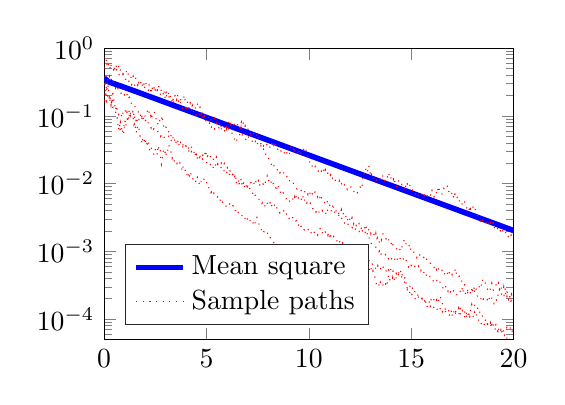
\begin{tikzpicture}

%\ begin{axis}[%
% width=5.706cm,
% height=4cm,
% at={(0cm,0cm)},
% scale only axis,
% xmin=0,
% xmax=20,
% ymode=log,
% ymin=1e-05,
% ymax=1,
% yminorticks=true,
% axis background/.style={fill=white},
% title style={font=\bfseries},
% title={reduced order controller},
% legend style={legend cell align=left, align=left, draw=white!15!black}
% ]
\begin{axis}[%
width=5.2cm,
height=3.7cm,
at={(0cm,0cm)},
scale only axis,
xmin=0,
xmax=20,
ymin=5e-05,
ymax=1,
ymode=log,
axis background/.style={fill=white},
legend style={at={(0.05,0.05)}, anchor=south west, legend cell align=left, align=left, draw=white!15!black}
]
\addplot [color=blue, line width=2.0pt]
  table[row sep=crcr]{%
0	0.36339119680705\\
0.202020202020202	0.320459400194069\\
0.404040404040404	0.304210969000361\\
0.606060606060606	0.290101900597729\\
0.808080808080808	0.276362027891353\\
1.01010101010101	0.262956704191335\\
1.21212121212121	0.25000285620796\\
1.41414141414141	0.237573501844568\\
1.61616161616162	0.225697318093611\\
1.81818181818182	0.214376894575785\\
2.02020202020202	0.203601313957933\\
2.22222222222222	0.193353043994078\\
2.42424242424242	0.183611502062773\\
2.62626262626263	0.174354892394527\\
2.82828282828283	0.165561170942239\\
3.03030303030303	0.157208564980986\\
3.23232323232323	0.14927585824784\\
3.43434343434343	0.141742547305093\\
3.63636363636364	0.134588923887381\\
3.83838383838384	0.127796112906742\\
4.04040404040404	0.121346083030465\\
4.24242424242424	0.115221639969157\\
4.44444444444444	0.109406408822842\\
4.64646464646465	0.103884809598938\\
4.84848484848485	0.0986420286323177\\
5.05050505050505	0.0936639877452251\\
5.25252525252525	0.0889373123906408\\
5.45454545454545	0.0844492996192829\\
5.65656565656566	0.0801878864314219\\
5.85858585858586	0.0761416188819059\\
6.06060606060606	0.0722996221716069\\
6.26262626262626	0.0686515718654088\\
6.46464646464646	0.0651876663112406\\
6.66666666666667	0.0618986002906416\\
6.86868686868687	0.0587755399007668\\
7.07070707070707	0.055810098647762\\
7.27272727272727	0.0529943147182152\\
7.47474747474747	0.0503206293875001\\
7.67676767676768	0.0477818665187611\\
7.87878787878788	0.0453712131049015\\
8.08080808080808	0.0430822008041114\\
8.28282828282828	0.0409086884209992\\
8.48484848484848	0.038844845285576\\
8.68686868686869	0.036885135485031\\
8.88888888888889	0.0350243029037932\\
9.09090909090909	0.033257357030343\\
9.29292929292929	0.0315795594907355\\
9.49494949494949	0.0299864112710885\\
9.6969696969697	0.0284736405929829\\
9.8989898989899	0.0270371914079603\\
10.1010101010101	0.025673212478328\\
10.3030303030303	0.024378047014855\\
10.5050505050505	0.0231482228413837\\
10.7070707070707	0.0219804430599352\\
10.9090909090909	0.0208715771896477\\
11.1111111111111	0.0198186527562416\\
11.3131313131313	0.0188188473077753\\
11.5151515151515	0.0178694808353933\\
11.7171717171717	0.0169680085780967\\
11.9191919191919	0.016112014192076\\
12.1212121212121	0.0152992032658071\\
12.3232323232323	0.0145273971636103\\
12.5252525252525	0.0137945271798698\\
12.7272727272727	0.0130986289900284\\
12.9292929292929	0.0124378373812559\\
13.1313131313131	0.0118103812500749\\
13.3333333333333	0.0112145788519433\\
13.5353535353535	0.010648833291947\\
13.7373737373737	0.0101116282425513\\
13.9393939393939	0.00960152387784802\\
14.1414141414141	0.0091171530130262\\
14.3434343434343	0.00865721743891272\\
14.5454545454545	0.00822048444151122\\
14.7474747474747	0.00780578349772744\\
14.9494949494949	0.00741200313640805\\
15.1515151515152	0.00703808795988641\\
15.3535353535354	0.00668303581428288\\
15.5555555555556	0.00634589510368296\\
15.7575757575758	0.00602576223838984\\
15.959595959596	0.00572177921382537\\
16.1616161616162	0.00543313131040472\\
16.3636363636364	0.00515904490975712\\
16.5656565656566	0.00489878542103152\\
16.7676767676768	0.00465165531195692\\
16.969696969697	0.00441699223924318\\
17.1717171717172	0.00419416727415203\\
17.3737373737374	0.00398258321484887\\
17.5757575757576	0.00378167298765328\\
17.7777777777778	0.00359089812616232\\
17.979797979798	0.00340974732894319\\
18.1818181818182	0.00323773508745117\\
18.3838383838384	0.0030744003863354\\
18.5858585858586	0.00291930546740519\\
18.7878787878788	0.00277203465627838\\
18.989898989899	0.00263219324817721\\
19.1919191919192	0.00249940644992965\\
19.3939393939394	0.00237331837556102\\
19.5959595959596	0.00225359109401439\\
19.7979797979798	0.00213990371987221\\
20	0.0020319515566487\\
};
\addlegendentry{Mean square}

\addplot [color=red, dotted]
  table[row sep=crcr]{%
0	0.733104233847529\\
0.02002002002002	0.646324787221493\\
0.04004004004004	0.648874736859844\\
0.0600600600600601	0.652843339128975\\
0.0800800800800801	0.647684873772235\\
0.1001001001001	0.675053831771465\\
0.12012012012012	0.647706328716021\\
0.14014014014014	0.632460633302073\\
0.16016016016016	0.656232145204731\\
0.18018018018018	0.620461162340896\\
0.2002002002002	0.585275923830458\\
0.22022022022022	0.560042853944174\\
0.24024024024024	0.54535179567966\\
0.26026026026026	0.528369909031415\\
0.28028028028028	0.565187527304748\\
0.3003003003003	0.553471746706723\\
0.32032032032032	0.565189281454622\\
0.34034034034034	0.556408687050879\\
0.36036036036036	0.536078839425328\\
0.38038038038038	0.53553390553816\\
0.4004004004004	0.526327280628495\\
0.42042042042042	0.527013978505917\\
0.44044044044044	0.514146594033145\\
0.46046046046046	0.500618066044095\\
0.48048048048048	0.503563767995262\\
0.500500500500501	0.517953989970728\\
0.520520520520521	0.503725071672013\\
0.540540540540541	0.535068588911094\\
0.560560560560561	0.496638291181907\\
0.580580580580581	0.506954660808583\\
0.600600600600601	0.562688509624717\\
0.620620620620621	0.561443605434184\\
0.640640640640641	0.592391076592891\\
0.660660660660661	0.577495771399926\\
0.680680680680681	0.57272961598051\\
0.700700700700701	0.55083886600988\\
0.720720720720721	0.531126975111277\\
0.740740740740741	0.484617231669433\\
0.760760760760761	0.483804465476424\\
0.780780780780781	0.505911023858578\\
0.800800800800801	0.467127204494059\\
0.820820820820821	0.444075933443123\\
0.840840840840841	0.439640325807461\\
0.860860860860861	0.447595110889789\\
0.880880880880881	0.432906547427056\\
0.900900900900901	0.425151221944503\\
0.920920920920921	0.407774253747736\\
0.940940940940941	0.412396098742461\\
0.960960960960961	0.416138000966063\\
0.980980980980981	0.43202154141227\\
1.001001001001	0.421805627059937\\
1.02102102102102	0.416603331992292\\
1.04104104104104	0.430615770989305\\
1.06106106106106	0.425779037394344\\
1.08108108108108	0.433524752781712\\
1.1011011011011	0.478138166463395\\
1.12112112112112	0.479326863416499\\
1.14114114114114	0.447517260975407\\
1.16116116116116	0.421833224771297\\
1.18118118118118	0.412944110746715\\
1.2012012012012	0.404494366522619\\
1.22122122122122	0.405381059599551\\
1.24124124124124	0.391950189452\\
1.26126126126126	0.376542194839096\\
1.28128128128128	0.372835977589905\\
1.3013013013013	0.387331763450652\\
1.32132132132132	0.351663192413488\\
1.34134134134134	0.340146089661392\\
1.36136136136136	0.346700108484984\\
1.38138138138138	0.346640422363531\\
1.4014014014014	0.361043244417345\\
1.42142142142142	0.381164082486361\\
1.44144144144144	0.361556538711018\\
1.46146146146146	0.36440679578785\\
1.48148148148148	0.361038398972964\\
1.5015015015015	0.365909328914583\\
1.52152152152152	0.384601812066819\\
1.54154154154154	0.362870532989338\\
1.56156156156156	0.347004454951122\\
1.58158158158158	0.348933038434176\\
1.6016016016016	0.352362635331609\\
1.62162162162162	0.355508514804708\\
1.64164164164164	0.336003125780376\\
1.66166166166166	0.333751825084097\\
1.68168168168168	0.323134323211657\\
1.7017017017017	0.30965547177567\\
1.72172172172172	0.315620612155368\\
1.74174174174174	0.317418241419258\\
1.76176176176176	0.312185898483676\\
1.78178178178178	0.308616740255619\\
1.8018018018018	0.306418694091679\\
1.82182182182182	0.310092223608482\\
1.84184184184184	0.289486298888855\\
1.86186186186186	0.285186648194899\\
1.88188188188188	0.282570196978801\\
1.9019019019019	0.274386240704288\\
1.92192192192192	0.265298438080758\\
1.94194194194194	0.255106447271383\\
1.96196196196196	0.246696383628363\\
1.98198198198198	0.263895358580493\\
2.002002002002	0.272442182203746\\
2.02202202202202	0.266671614624832\\
2.04204204204204	0.253075000879924\\
2.06206206206206	0.252173486768017\\
2.08208208208208	0.246415050868938\\
2.1021021021021	0.245240639856551\\
2.12212212212212	0.243269196971854\\
2.14214214214214	0.24138632307485\\
2.16216216216216	0.237394035948291\\
2.18218218218218	0.239827814368119\\
2.2022022022022	0.232861255595684\\
2.22222222222222	0.218491587245214\\
2.24224224224224	0.225429634231494\\
2.26226226226226	0.222113988305373\\
2.28228228228228	0.240679837970539\\
2.3023023023023	0.261359810387614\\
2.32232232232232	0.247184042889173\\
2.34234234234234	0.244665531599794\\
2.36236236236236	0.256796745400897\\
2.38238238238238	0.280448261472847\\
2.4024024024024	0.259074932305065\\
2.42242242242242	0.253628354959198\\
2.44244244244244	0.258435935390615\\
2.46246246246246	0.240960524410921\\
2.48248248248248	0.235127048149145\\
2.5025025025025	0.236623903555889\\
2.52252252252252	0.23110659359802\\
2.54254254254254	0.237094241512083\\
2.56256256256256	0.240379064048399\\
2.58258258258258	0.236397857121703\\
2.6026026026026	0.236497910375081\\
2.62262262262262	0.222986049941444\\
2.64264264264264	0.220129732565191\\
2.66266266266266	0.224118019302236\\
2.68268268268268	0.220611994476894\\
2.7027027027027	0.216731870595339\\
2.72272272272272	0.221055162489879\\
2.74274274274274	0.21299334441804\\
2.76276276276276	0.204170353774316\\
2.78278278278278	0.210584345280858\\
2.8028028028028	0.209384828825948\\
2.82282282282282	0.203648590231945\\
2.84284284284284	0.204850604127984\\
2.86286286286286	0.198334820406017\\
2.88288288288288	0.208228685722417\\
2.9029029029029	0.222432771979531\\
2.92292292292292	0.211581957285724\\
2.94294294294294	0.20812633744656\\
2.96296296296296	0.198297882596698\\
2.98298298298298	0.180998810093551\\
3.003003003003	0.180321849281916\\
3.02302302302302	0.17393109455088\\
3.04304304304304	0.183467355556575\\
3.06306306306306	0.208426922422713\\
3.08308308308308	0.209587708023864\\
3.1031031031031	0.201649673606504\\
3.12312312312312	0.194673926990055\\
3.14314314314314	0.191612711053164\\
3.16316316316316	0.186020320260605\\
3.18318318318318	0.194103989661246\\
3.2032032032032	0.195352891824109\\
3.22322322322322	0.189167223157284\\
3.24324324324324	0.178894144573103\\
3.26326326326326	0.175851352822831\\
3.28328328328328	0.172828650003485\\
3.3033033033033	0.173940840299181\\
3.32332332332332	0.158140252188697\\
3.34334334334334	0.156404793547541\\
3.36336336336336	0.166261210770458\\
3.38338338338338	0.155382318358075\\
3.4034034034034	0.159705364051133\\
3.42342342342342	0.15504471743582\\
3.44344344344344	0.152435319975499\\
3.46346346346346	0.152115393324235\\
3.48348348348348	0.149965229237072\\
3.5035035035035	0.152402371740822\\
3.52352352352352	0.160116898715172\\
3.54354354354354	0.170049537999229\\
3.56356356356356	0.160390699022067\\
3.58358358358358	0.164156185883334\\
3.6036036036036	0.16153957726562\\
3.62362362362362	0.153755674163255\\
3.64364364364364	0.165578832023943\\
3.66366366366366	0.164785912875266\\
3.68368368368368	0.167959227033525\\
3.7037037037037	0.176464028721037\\
3.72372372372372	0.170307714832777\\
3.74374374374374	0.152101819266005\\
3.76376376376376	0.140947727898517\\
3.78378378378378	0.131623257277787\\
3.8038038038038	0.129041804663805\\
3.82382382382382	0.129762829196831\\
3.84384384384384	0.130760212839099\\
3.86386386386386	0.129442818671942\\
3.88388388388388	0.131368893436991\\
3.9039039039039	0.123915864042607\\
3.92392392392392	0.125502614588774\\
3.94394394394394	0.123893837948406\\
3.96396396396396	0.128574300739964\\
3.98398398398398	0.130876476515256\\
4.004004004004	0.129423979236743\\
4.02402402402402	0.128715980010094\\
4.04404404404404	0.135439923340952\\
4.06406406406406	0.1286954445889\\
4.08408408408408	0.130707533997713\\
4.1041041041041	0.135808187515971\\
4.12412412412412	0.132729777064482\\
4.14414414414414	0.132014255946762\\
4.16416416416416	0.129640853376474\\
4.18418418418418	0.134473632355864\\
4.2042042042042	0.135449570685669\\
4.22422422422422	0.134223391011982\\
4.24424424424424	0.129257930704881\\
4.26426426426426	0.121175328602405\\
4.28428428428428	0.122435213237981\\
4.3043043043043	0.133097683080687\\
4.32432432432432	0.131703418998291\\
4.34434434434434	0.126403549999838\\
4.36436436436436	0.11975343816176\\
4.38438438438438	0.114426602027332\\
4.4044044044044	0.10676626651513\\
4.42442442442442	0.102525856537497\\
4.44444444444444	0.0994862116199186\\
4.46446446446446	0.10337564851745\\
4.48448448448448	0.103918055595807\\
4.5045045045045	0.103240691470709\\
4.52452452452452	0.101197477722414\\
4.54454454454454	0.103124804571072\\
4.56456456456456	0.102757615889668\\
4.58458458458458	0.102624653463783\\
4.6046046046046	0.0999154662735517\\
4.62462462462462	0.0996301275224384\\
4.64464464464464	0.106011354021387\\
4.66466466466466	0.105487380038022\\
4.68468468468468	0.104388264895043\\
4.7047047047047	0.101779935365216\\
4.72472472472472	0.102768721376176\\
4.74474474474474	0.0993270707074693\\
4.76476476476476	0.0991040936157664\\
4.78478478478478	0.104418964872559\\
4.8048048048048	0.101347948839176\\
4.82482482482482	0.0963689001982036\\
4.84484484484484	0.09122594303528\\
4.86486486486486	0.0866955004386361\\
4.88488488488488	0.0839768958114943\\
4.9049049049049	0.0847591843627837\\
4.92492492492492	0.0849748273531898\\
4.94494494494494	0.0852244230455547\\
4.96496496496496	0.0858228344798328\\
4.98498498498498	0.0829049006306614\\
5.00500500500501	0.0836269725938935\\
5.02502502502503	0.0822024470762569\\
5.04504504504505	0.0803468610583171\\
5.06506506506507	0.0763576736011506\\
5.08508508508509	0.0773683999271199\\
5.10510510510511	0.0787678596963892\\
5.12512512512513	0.0782605841814763\\
5.14514514514515	0.0784494382809719\\
5.16516516516517	0.0750861525650623\\
5.18518518518519	0.0765517195885987\\
5.20520520520521	0.069656566715812\\
5.22522522522523	0.0669819435214521\\
5.24524524524525	0.068479884451265\\
5.26526526526527	0.0660417454262531\\
5.28528528528529	0.0644596120871943\\
5.30530530530531	0.0613012459900482\\
5.32532532532533	0.0639494682656243\\
5.34534534534535	0.0627864930636039\\
5.36536536536537	0.0636326336420395\\
5.38538538538539	0.063353265040748\\
5.40540540540541	0.0646141991762518\\
5.42542542542543	0.0649084472106362\\
5.44544544544545	0.0666502191817635\\
5.46546546546547	0.067302230797479\\
5.48548548548549	0.0656610751991055\\
5.50550550550551	0.0656024397315401\\
5.52552552552553	0.0668308205208545\\
5.54554554554555	0.0671022063405107\\
5.56556556556557	0.0686597615916669\\
5.58558558558559	0.0669860555746745\\
5.60560560560561	0.0669752473055671\\
5.62562562562563	0.0620406903029936\\
5.64564564564565	0.0621315717652625\\
5.66566566566567	0.0648604744293264\\
5.68568568568569	0.0668912799912144\\
5.70570570570571	0.0692708825783204\\
5.72572572572573	0.072855501198459\\
5.74574574574575	0.070486334835373\\
5.76576576576577	0.0684231966762732\\
5.78578578578579	0.0702290953011452\\
5.80580580580581	0.0677892109423976\\
5.82582582582583	0.0672595322668339\\
5.84584584584585	0.0684885166787946\\
5.86586586586587	0.0681977790357591\\
5.88588588588589	0.0681110525953407\\
5.90590590590591	0.0700779951380513\\
5.92592592592593	0.0718848302333859\\
5.94594594594595	0.0754012949908703\\
5.96596596596597	0.0751247162789525\\
5.98598598598599	0.0695371903779407\\
6.00600600600601	0.0640090881534784\\
6.02602602602603	0.0654637301497388\\
6.04604604604605	0.0617294527222122\\
6.06606606606607	0.0611652029095005\\
6.08608608608609	0.0642771917350877\\
6.10610610610611	0.0624760734705456\\
6.12612612612613	0.0617726261273519\\
6.14614614614615	0.0616473191326485\\
6.16616616616617	0.0597246887158464\\
6.18618618618619	0.0580497036598444\\
6.20620620620621	0.0581845805336813\\
6.22622622622623	0.0549425083554071\\
6.24624624624625	0.0556343732592686\\
6.26626626626627	0.0546834013009815\\
6.28628628628629	0.0519713736601609\\
6.30630630630631	0.0510730248886072\\
6.32632632632633	0.0492144137016396\\
6.34634634634635	0.0490871079982742\\
6.36636636636637	0.0468961281273285\\
6.38638638638639	0.0429950052910337\\
6.40640640640641	0.0442409762615302\\
6.42642642642643	0.0421601235384033\\
6.44644644644645	0.0415084570087052\\
6.46646646646647	0.0418263104392149\\
6.48648648648649	0.0449650710256941\\
6.50650650650651	0.0456654484169152\\
6.52652652652653	0.046110873866772\\
6.54654654654655	0.047275103764353\\
6.56656656656657	0.0489327403306754\\
6.58658658658659	0.050145945202876\\
6.60660660660661	0.0501568964856492\\
6.62662662662663	0.0530931303128895\\
6.64664664664665	0.0549211052543004\\
6.66666666666667	0.0585165240024441\\
6.68668668668669	0.065270899000937\\
6.70670670670671	0.0561582662676225\\
6.72672672672673	0.054644717157587\\
6.74674674674675	0.0524284852824129\\
6.76676676676677	0.0525594971231588\\
6.78678678678679	0.0512998312640432\\
6.80680680680681	0.0521585798121975\\
6.82682682682683	0.0509210396081663\\
6.84684684684685	0.0474224622643004\\
6.86686686686687	0.0471605344495846\\
6.88688688688689	0.0458970361491707\\
6.90690690690691	0.0452813181036726\\
6.92692692692693	0.0451051156785923\\
6.94694694694695	0.0468265076882736\\
6.96696696696697	0.0474708514957289\\
6.98698698698699	0.0449122418837148\\
7.00700700700701	0.0469299553743505\\
7.02702702702703	0.0470186392596718\\
7.04704704704705	0.0479998741438872\\
7.06706706706707	0.0512754402706688\\
7.08708708708709	0.0503288734488626\\
7.10710710710711	0.0520629447401828\\
7.12712712712713	0.0515941981135977\\
7.14714714714715	0.0511869895641337\\
7.16716716716717	0.0540457496837983\\
7.18718718718719	0.0476634795131028\\
7.20720720720721	0.0470474492700719\\
7.22722722722723	0.0442455728041362\\
7.24724724724725	0.0414815951798581\\
7.26726726726727	0.0405078689239448\\
7.28728728728729	0.0416608559599172\\
7.30730730730731	0.0416137152303799\\
7.32732732732733	0.0422757666760322\\
7.34734734734735	0.0418127703510904\\
7.36736736736737	0.0437385185656794\\
7.38738738738739	0.0421980479994819\\
7.40740740740741	0.0435117312721763\\
7.42742742742743	0.0415457701505205\\
7.44744744744745	0.0410776964606529\\
7.46746746746747	0.0427440363743657\\
7.48748748748749	0.0396910165122667\\
7.50750750750751	0.0379111384204438\\
7.52752752752753	0.038233738261732\\
7.54754754754755	0.035662680903473\\
7.56756756756757	0.0350421866449373\\
7.58758758758759	0.0346107265356421\\
7.60760760760761	0.0349679181614901\\
7.62762762762763	0.0355278971342948\\
7.64764764764765	0.0359945747396434\\
7.66766766766767	0.0360036556508681\\
7.68768768768769	0.0343921970336499\\
7.70770770770771	0.0324841852137664\\
7.72772772772773	0.0316483598711281\\
7.74774774774775	0.0320009890545102\\
7.76776776776777	0.0311284088700877\\
7.78778778778779	0.0322318333770405\\
7.80780780780781	0.0316374181037555\\
7.82782782782783	0.0307619631111137\\
7.84784784784785	0.0291288800579017\\
7.86786786786787	0.0276781789869509\\
7.88788788788789	0.0282178542822796\\
7.90790790790791	0.0266048436517283\\
7.92792792792793	0.0258441192604274\\
7.94794794794795	0.0263330422735005\\
7.96796796796797	0.0251814328309119\\
7.98798798798799	0.0246012124499184\\
8.00800800800801	0.0237750978203564\\
8.02802802802803	0.0238979427027936\\
8.04804804804805	0.0233919497765359\\
8.06806806806807	0.0224323316570198\\
8.08808808808809	0.0216774095576942\\
8.10810810810811	0.0213602676254787\\
8.12812812812813	0.020468307481789\\
8.14814814814815	0.0204628786018624\\
8.16816816816817	0.0192940844056475\\
8.18818818818819	0.0185911401483858\\
8.20820820820821	0.0180373945469657\\
8.22822822822823	0.017223455607493\\
8.24824824824825	0.0179432730848965\\
8.26826826826827	0.0177241269710703\\
8.28828828828829	0.0182695061892371\\
8.30830830830831	0.0183175212094267\\
8.32832832832833	0.0182499734085894\\
8.34834834834835	0.016936667679894\\
8.36836836836837	0.0165357370767977\\
8.38838838838839	0.0162610068846762\\
8.40840840840841	0.0161277215237178\\
8.42842842842843	0.0164878747064878\\
8.44844844844845	0.0163333203415533\\
8.46846846846847	0.0158570021127674\\
8.48848848848849	0.0153727432315282\\
8.50850850850851	0.0147856097814878\\
8.52852852852853	0.0150918035416001\\
8.54854854854855	0.0146957685652733\\
8.56856856856857	0.0150539314668732\\
8.58858858858859	0.0144479393407317\\
8.60860860860861	0.0147947727313316\\
8.62862862862863	0.0148162704254953\\
8.64864864864865	0.0144118720558524\\
8.66866866866867	0.0142110094844333\\
8.68868868868869	0.0146256603268992\\
8.70870870870871	0.0146158544689283\\
8.72872872872873	0.0143524628455238\\
8.74874874874875	0.0144763250890107\\
8.76876876876877	0.0148379896096965\\
8.78878878878879	0.014013020465584\\
8.80880880880881	0.0138177632684518\\
8.82882882882883	0.0141172230502025\\
8.84884884884885	0.0136740522935021\\
8.86886886886887	0.0133411066787458\\
8.88888888888889	0.0135546435403659\\
8.90890890890891	0.0132908536711224\\
8.92892892892893	0.0127630808853839\\
8.94894894894895	0.0123507497317601\\
8.96896896896897	0.0116741917584231\\
8.98898898898899	0.0115376111926003\\
9.00900900900901	0.0118994244509965\\
9.02902902902903	0.0116628461918834\\
9.04904904904905	0.0112145241305317\\
9.06906906906907	0.0108356972213177\\
9.08908908908909	0.0107013729267834\\
9.10910910910911	0.0106632106970798\\
9.12912912912913	0.010497083776603\\
9.14914914914915	0.0106722402707614\\
9.16916916916917	0.0105409610250021\\
9.18918918918919	0.0103909480055398\\
9.20920920920921	0.0106752734528817\\
9.22922922922923	0.0104847716163646\\
9.24924924924925	0.0101288533295413\\
9.26926926926927	0.00973458693532372\\
9.28928928928929	0.00973583933785714\\
9.30930930930931	0.0095356092724532\\
9.32932932932933	0.0093663898738892\\
9.34934934934935	0.00928043155657876\\
9.36936936936937	0.0087720155626611\\
9.38938938938939	0.00857809262009112\\
9.40940940940941	0.00846752975260821\\
9.42942942942943	0.00835672635542383\\
9.44944944944945	0.00848860643431547\\
9.46946946946947	0.00843843516848113\\
9.48948948948949	0.0084820369644348\\
9.50950950950951	0.00850804932769392\\
9.52952952952953	0.00850953700707989\\
9.54954954954955	0.00816602595882144\\
9.56956956956957	0.00804494229528445\\
9.58958958958959	0.00780259552996382\\
9.60960960960961	0.00785590637467294\\
9.62962962962963	0.00797367312371569\\
9.64964964964965	0.00807766408582368\\
9.66966966966967	0.00799948341896548\\
9.68968968968969	0.0077636424965898\\
9.70970970970971	0.00762344787047755\\
9.72972972972973	0.00755269026138071\\
9.74974974974975	0.00759813198944962\\
9.76976976976977	0.00726029534417504\\
9.78978978978979	0.00740881421754853\\
9.80980980980981	0.00776569050548932\\
9.82982982982983	0.0077919314115264\\
9.84984984984985	0.00753496367672915\\
9.86986986986987	0.00742127512952037\\
9.88988988988989	0.00708528437879415\\
9.90990990990991	0.00706436461267599\\
9.92992992992993	0.00714866644721461\\
9.94994994994995	0.00694857529805108\\
9.96996996996997	0.00739214089416805\\
9.98998998998999	0.00776908402216677\\
10.01001001001	0.00795043086613859\\
10.03003003003	0.00775998090774116\\
10.0500500500501	0.0073902281799479\\
10.0700700700701	0.00697260255411871\\
10.0900900900901	0.00708513058756169\\
10.1101101101101	0.00697415889805334\\
10.1301301301301	0.00723380070225249\\
10.1501501501502	0.0075580868348668\\
10.1701701701702	0.00710022423516943\\
10.1901901901902	0.00725275377279765\\
10.2102102102102	0.00703826377635402\\
10.2302302302302	0.00671644887187606\\
10.2502502502503	0.00698154026813525\\
10.2702702702703	0.00715323555384806\\
10.2902902902903	0.00748594883346823\\
10.3103103103103	0.0075143206749389\\
10.3303303303303	0.00724017736767818\\
10.3503503503504	0.00694848350333533\\
10.3703703703704	0.00707782046098386\\
10.3903903903904	0.00708450538502001\\
10.4104104104104	0.00678471874364821\\
10.4304304304304	0.00640478686675507\\
10.4504504504505	0.00665352556866311\\
10.4704704704705	0.00663351790348544\\
10.4904904904905	0.00666200477762849\\
10.5105105105105	0.00692061492444864\\
10.5305305305305	0.00658998148250801\\
10.5505505505506	0.00600742597676722\\
10.5705705705706	0.00570244019994454\\
10.5905905905906	0.00593515761920314\\
10.6106106106106	0.00631076973423984\\
10.6306306306306	0.00602428305379444\\
10.6506506506507	0.00566285164358482\\
10.6706706706707	0.00571326547838656\\
10.6906906906907	0.00555206833750536\\
10.7107107107107	0.00552911664725114\\
10.7307307307307	0.00556831770944402\\
10.7507507507508	0.00543098687596645\\
10.7707707707708	0.00524744333632487\\
10.7907907907908	0.00521162117118063\\
10.8108108108108	0.00563703896160955\\
10.8308308308308	0.00538926379783003\\
10.8508508508509	0.00546594963400707\\
10.8708708708709	0.00535287851502732\\
10.8908908908909	0.005425991429914\\
10.9109109109109	0.00541314135342665\\
10.9309309309309	0.00521711136580623\\
10.950950950951	0.00506212946216984\\
10.970970970971	0.00509236781696024\\
10.990990990991	0.00474922919582987\\
11.011011011011	0.0049251463311347\\
11.031031031031	0.00468264786916051\\
11.0510510510511	0.00447699924661792\\
11.0710710710711	0.00456681378237732\\
11.0910910910911	0.00467601265829983\\
11.1111111111111	0.00479933256698556\\
11.1311311311311	0.00488381538068394\\
11.1511511511512	0.00476654271544358\\
11.1711711711712	0.00444829260155111\\
11.1911911911912	0.00421749448071677\\
11.2112112112112	0.0039945117976969\\
11.2312312312312	0.00386722576039201\\
11.2512512512513	0.00380648019450236\\
11.2712712712713	0.00379751444609755\\
11.2912912912913	0.00370474313128525\\
11.3113113113113	0.00369754541368619\\
11.3313313313313	0.0035932580556503\\
11.3513513513514	0.00352807055588897\\
11.3713713713714	0.00352986229491975\\
11.3913913913914	0.00349990002702423\\
11.4114114114114	0.00341762362326738\\
11.4314314314314	0.00331620254129595\\
11.4514514514515	0.00339806776501319\\
11.4714714714715	0.0033926383565145\\
11.4914914914915	0.00332903608501455\\
11.5115115115115	0.00319437458939731\\
11.5315315315315	0.00318663866051885\\
11.5515515515516	0.00330792836848774\\
11.5715715715716	0.00313356951518569\\
11.5915915915916	0.00313294178112438\\
11.6116116116116	0.00298440672063483\\
11.6316316316316	0.00289518702374802\\
11.6516516516517	0.00284419832748993\\
11.6716716716717	0.00285937537542763\\
11.6916916916917	0.00272107128965492\\
11.7117117117117	0.00267802082031227\\
11.7317317317317	0.00272288248489136\\
11.7517517517518	0.00260926008344236\\
11.7717717717718	0.0026115141550606\\
11.7917917917918	0.00260583449086567\\
11.8118118118118	0.00270326439850484\\
11.8318318318318	0.002551838621704\\
11.8518518518519	0.00253367889184356\\
11.8718718718719	0.00257693706228122\\
11.8918918918919	0.00259485436800573\\
11.9119119119119	0.00253734060254952\\
11.9319319319319	0.00245838179136782\\
11.951951951952	0.00243974531328843\\
11.971971971972	0.00241430781919479\\
11.991991991992	0.00239032710152003\\
12.012012012012	0.00234727614460387\\
12.032032032032	0.00240179715545703\\
12.0520520520521	0.00240317844007935\\
12.0720720720721	0.00242233500333748\\
12.0920920920921	0.00233083345205139\\
12.1121121121121	0.0022722066749313\\
12.1321321321321	0.00224081556667521\\
12.1521521521522	0.00229456199836441\\
12.1721721721722	0.00222904623907407\\
12.1921921921922	0.00212909161503994\\
12.2122122122122	0.00209888912955662\\
12.2322322322322	0.00217919333865749\\
12.2522522522523	0.00217644024747384\\
12.2722722722723	0.00212817891979859\\
12.2922922922923	0.00214299405749405\\
12.3123123123123	0.00212899833614844\\
12.3323323323323	0.00208387192903894\\
12.3523523523524	0.00210383308822314\\
12.3723723723724	0.00209712727181881\\
12.3923923923924	0.00204991106110956\\
12.4124124124124	0.00199413756255093\\
12.4324324324324	0.00194421539152389\\
12.4524524524525	0.00190878512389077\\
12.4724724724725	0.00198702638391658\\
12.4924924924925	0.00198359188917644\\
12.5125125125125	0.00190930798216796\\
12.5325325325325	0.0019227507030103\\
12.5525525525526	0.00186171366627455\\
12.5725725725726	0.00198074010252926\\
12.5925925925926	0.00199351472668097\\
12.6126126126126	0.00199096847276785\\
12.6326326326326	0.00209932529108704\\
12.6526526526527	0.00204363016335632\\
12.6726726726727	0.00210225984349558\\
12.6926926926927	0.00210596152633925\\
12.7127127127127	0.002061814702689\\
12.7327327327327	0.00200079607931222\\
12.7527527527528	0.00192086574691175\\
12.7727727727728	0.00178827188051451\\
12.7927927927928	0.00175104348601123\\
12.8128128128128	0.00187181873972602\\
12.8328328328328	0.00179617687013882\\
12.8528528528529	0.00181577101244785\\
12.8728728728729	0.00188718300562598\\
12.8928928928929	0.00183183629661438\\
12.9129129129129	0.00170948862186994\\
12.9329329329329	0.00167436135513755\\
12.952952952953	0.00157452478548967\\
12.972972972973	0.00150822045282264\\
12.992992992993	0.00141203796535259\\
13.013013013013	0.00142851745281624\\
13.033033033033	0.00139946683237774\\
13.0530530530531	0.00129693828664566\\
13.0730730730731	0.00126700887401254\\
13.0930930930931	0.00125153887246086\\
13.1131131131131	0.00122837002505338\\
13.1331331331331	0.00121628715943818\\
13.1531531531532	0.00120087992939492\\
13.1731731731732	0.0012001960119375\\
13.1931931931932	0.00121370935667951\\
13.2132132132132	0.00119506848585352\\
13.2332332332332	0.00119198842568508\\
13.2532532532533	0.00116813379856334\\
13.2732732732733	0.00115455607454767\\
13.2932932932933	0.00117581021314933\\
13.3133133133133	0.00114163594246956\\
13.3333333333333	0.00110696575088265\\
13.3533533533534	0.0010985803151085\\
13.3733733733734	0.00109409936709408\\
13.3933933933934	0.00107704549162991\\
13.4134134134134	0.00104974445806846\\
13.4334334334334	0.000996932741154828\\
13.4534534534535	0.00101514368007401\\
13.4734734734735	0.000969084769943661\\
13.4934934934935	0.00101483116381414\\
13.5135135135135	0.0009437006462832\\
13.5335335335335	0.00090456618702333\\
13.5535535535536	0.000868179458383148\\
13.5735735735736	0.000877817433398406\\
13.5935935935936	0.00086842850235105\\
13.6136136136136	0.000855635157393545\\
13.6336336336336	0.00085623804816999\\
13.6536536536537	0.000844179588098102\\
13.6736736736737	0.000868047892690449\\
13.6936936936937	0.000876945331967037\\
13.7137137137137	0.000877866645319617\\
13.7337337337337	0.00088779317476192\\
13.7537537537538	0.00090099103276715\\
13.7737737737738	0.000873953640458145\\
13.7937937937938	0.000874001300483571\\
13.8138138138138	0.00087962156382458\\
13.8338338338338	0.000848932136877231\\
13.8538538538539	0.000792907214721061\\
13.8738738738739	0.000799397904197284\\
13.8938938938939	0.00077785832089039\\
13.9139139139139	0.0007840448347959\\
13.9339339339339	0.000777633052588363\\
13.953953953954	0.000804343298605534\\
13.973973973974	0.000770846376928215\\
13.993993993994	0.000741323777907445\\
14.014014014014	0.000752738189252773\\
14.034034034034	0.000756641813010842\\
14.0540540540541	0.000788309282468984\\
14.0740740740741	0.000789467573179549\\
14.0940940940941	0.000762344713128193\\
14.1141141141141	0.000751815952114343\\
14.1341341341341	0.00074494240308607\\
14.1541541541542	0.000715656416746893\\
14.1741741741742	0.000734582806758754\\
14.1941941941942	0.000741844275503198\\
14.2142142142142	0.000828812117474619\\
14.2342342342342	0.000822379626644167\\
14.2542542542543	0.000795128499169224\\
14.2742742742743	0.000772502358349599\\
14.2942942942943	0.000750160046488038\\
14.3143143143143	0.000760218968386315\\
14.3343343343343	0.00078105635280704\\
14.3543543543544	0.000778445152032748\\
14.3743743743744	0.000795802850361559\\
14.3943943943944	0.000768758094157081\\
14.4144144144144	0.00081585443124926\\
14.4344344344344	0.000822649550235871\\
14.4544544544545	0.000787625917831381\\
14.4744744744745	0.000788654018224113\\
14.4944944944945	0.000755945937093506\\
14.5145145145145	0.000747246666024664\\
14.5345345345345	0.000753634773171861\\
14.5545545545546	0.000775576530056872\\
14.5745745745746	0.000777735799017987\\
14.5945945945946	0.000808228035302349\\
14.6146146146146	0.0007836440444391\\
14.6346346346346	0.000751696113940561\\
14.6546546546547	0.00072388790885997\\
14.6746746746747	0.000714465023115918\\
14.6946946946947	0.000724022757785582\\
14.7147147147147	0.000723536442210376\\
14.7347347347347	0.00070536315892864\\
14.7547547547548	0.00074590152398112\\
14.7747747747748	0.000708163398175346\\
14.7947947947948	0.000695588967636128\\
14.8148148148148	0.000671795976633425\\
14.8348348348348	0.000649118790145715\\
14.8548548548549	0.00061176761368871\\
14.8748748748749	0.000589319549235305\\
14.8948948948949	0.000601240610616431\\
14.9149149149149	0.000588602736689059\\
14.9349349349349	0.000564845418405042\\
14.954954954955	0.000606821172776139\\
14.974974974975	0.000614934498192382\\
14.994994994995	0.000626425846275719\\
15.015015015015	0.000619187137205859\\
15.035035035035	0.000639492054226943\\
15.0550550550551	0.000642867970964003\\
15.0750750750751	0.000613374821438348\\
15.0950950950951	0.000617176619791565\\
15.1151151151151	0.000632334774799305\\
15.1351351351351	0.000630176173877303\\
15.1551551551552	0.000622263272482718\\
15.1751751751752	0.000601128033021823\\
15.1951951951952	0.000605111921804651\\
15.2152152152152	0.000600545656874845\\
15.2352352352352	0.000597914754378858\\
15.2552552552553	0.000594625380163653\\
15.2752752752753	0.000602381544357187\\
15.2952952952953	0.000574155720901639\\
15.3153153153153	0.000595888234898157\\
15.3353353353353	0.00058838008763444\\
15.3553553553554	0.000603302295519498\\
15.3753753753754	0.000578126530002838\\
15.3953953953954	0.000548169253966101\\
15.4154154154154	0.000541652324234678\\
15.4354354354354	0.000558855124538975\\
15.4554554554555	0.000566853979157622\\
15.4754754754755	0.000527205283384688\\
15.4954954954955	0.000552127359797585\\
15.5155155155155	0.000540898759150631\\
15.5355355355355	0.000525466452376577\\
15.5555555555556	0.000512584607901818\\
15.5755755755756	0.000518948076639787\\
15.5955955955956	0.000500155984840654\\
15.6156156156156	0.00049169606571432\\
15.6356356356356	0.00048318535125265\\
15.6556556556557	0.000472734238754898\\
15.6756756756757	0.000466872209454832\\
15.6956956956957	0.000443911184749276\\
15.7157157157157	0.000422828026055214\\
15.7357357357357	0.000445360787659013\\
15.7557557557558	0.000444338369874858\\
15.7757757757758	0.000436772953933975\\
15.7957957957958	0.000448878700871277\\
15.8158158158158	0.000443729857296349\\
15.8358358358358	0.000451625268686777\\
15.8558558558559	0.000449011799360435\\
15.8758758758759	0.000459054375496039\\
15.8958958958959	0.000454209607282888\\
15.9159159159159	0.000421706775378962\\
15.9359359359359	0.000404162005032151\\
15.955955955956	0.000400264766594595\\
15.975975975976	0.000405476810112827\\
15.995995995996	0.000395270258698523\\
16.016016016016	0.000396883770317785\\
16.036036036036	0.000395870467459361\\
16.0560560560561	0.000383520430488271\\
16.0760760760761	0.000367146218832714\\
16.0960960960961	0.000363009318328261\\
16.1161161161161	0.000359638898403275\\
16.1361361361361	0.000351153408666831\\
16.1561561561562	0.000361731571057003\\
16.1761761761762	0.00036458121159459\\
16.1961961961962	0.000372189673087075\\
16.2162162162162	0.000369698619142564\\
16.2362362362362	0.000384566482642727\\
16.2562562562563	0.00037070237457587\\
16.2762762762763	0.000365354401536901\\
16.2962962962963	0.000375004993863185\\
16.3163163163163	0.000360928706856962\\
16.3363363363363	0.00036215932980857\\
16.3563563563564	0.000352035683646647\\
16.3763763763764	0.00035669940143494\\
16.3963963963964	0.000364067938548805\\
16.4164164164164	0.000344868263962972\\
16.4364364364364	0.000337976190059403\\
16.4564564564565	0.000333144996947667\\
16.4764764764765	0.000334111318477324\\
16.4964964964965	0.000327072019505057\\
16.5165165165165	0.000316622688047449\\
16.5365365365365	0.000305577464227007\\
16.5565565565566	0.000284125238122022\\
16.5765765765766	0.000299200760396334\\
16.5965965965966	0.000309295643247766\\
16.6166166166166	0.000312868604351056\\
16.6366366366366	0.00031699140427915\\
16.6566566566567	0.00031792575915911\\
16.6766766766767	0.000313376064268866\\
16.6966966966967	0.000290280236236787\\
16.7167167167167	0.000274723667924623\\
16.7367367367367	0.000281475500673702\\
16.7567567567568	0.000269229080747187\\
16.7767767767768	0.000264922078846872\\
16.7967967967968	0.000258582763584085\\
16.8168168168168	0.000279101919330632\\
16.8368368368368	0.000283885907143904\\
16.8568568568569	0.000274717201038798\\
16.8768768768769	0.00026920712094159\\
16.8968968968969	0.000266821392516912\\
16.9169169169169	0.000262887357100275\\
16.9369369369369	0.00024974274182275\\
16.956956956957	0.000249179996202736\\
16.976976976977	0.000261485385045235\\
16.996996996997	0.000245426967539531\\
17.017017017017	0.000252632747988223\\
17.037037037037	0.000256418773661287\\
17.0570570570571	0.000258510261686432\\
17.0770770770771	0.000267982130865612\\
17.0970970970971	0.000263945571266689\\
17.1171171171171	0.000256595735226093\\
17.1371371371371	0.000255905703258388\\
17.1571571571572	0.000256380509901221\\
17.1771771771772	0.000245842968543783\\
17.1971971971972	0.000240289536311137\\
17.2172172172172	0.000237759710320903\\
17.2372372372372	0.000228689278307548\\
17.2572572572573	0.000226904335876067\\
17.2772772772773	0.000231183319879422\\
17.2972972972973	0.000231886316818991\\
17.3173173173173	0.000243886695347715\\
17.3373373373373	0.000245402887525137\\
17.3573573573574	0.000240731660039426\\
17.3773773773774	0.000250751217640943\\
17.3973973973974	0.000258111283394436\\
17.4174174174174	0.000269290119541291\\
17.4374374374374	0.000252734981570946\\
17.4574574574575	0.000270825298180989\\
17.4774774774775	0.000277432269600666\\
17.4974974974975	0.000282811136530962\\
17.5175175175175	0.000302298041858768\\
17.5375375375375	0.000267137146096925\\
17.5575575575576	0.000241875138058497\\
17.5775775775776	0.000249107384517611\\
17.5975975975976	0.000257567362274842\\
17.6176176176176	0.000254765164101943\\
17.6376376376376	0.00024783769852788\\
17.6576576576577	0.000234361671285045\\
17.6776776776777	0.000234342003598559\\
17.6976976976977	0.000229494604523598\\
17.7177177177177	0.000225820652842312\\
17.7377377377377	0.000238819637899687\\
17.7577577577578	0.000252055870010695\\
17.7777777777778	0.000233127687782442\\
17.7977977977978	0.000226768076031375\\
17.8178178178178	0.000236394753332088\\
17.8378378378378	0.000231399427822755\\
17.8578578578579	0.000234199723179089\\
17.8778778778779	0.000238599326047891\\
17.8978978978979	0.000246905683000718\\
17.9179179179179	0.000256248862780886\\
17.9379379379379	0.000276522055896165\\
17.957957957958	0.000265287603991633\\
17.977977977978	0.000265605025852294\\
17.997997997998	0.00026072243040092\\
18.018018018018	0.000273211245328353\\
18.038038038038	0.000292979136958445\\
18.0580580580581	0.000272249249724784\\
18.0780780780781	0.000297098336807884\\
18.0980980980981	0.000303282728293097\\
18.1181181181181	0.000300967345309444\\
18.1381381381381	0.000288203553494974\\
18.1581581581582	0.000270694652867747\\
18.1781781781782	0.000271045284617387\\
18.1981981981982	0.000293814868802802\\
18.2182182182182	0.000298514544714055\\
18.2382382382382	0.000303549001859356\\
18.2582582582583	0.000304073009331093\\
18.2782782782783	0.000290157058688223\\
18.2982982982983	0.000288602468565362\\
18.3183183183183	0.000298931846683861\\
18.3383383383383	0.000309372262786327\\
18.3583583583584	0.000329401740282685\\
18.3783783783784	0.000309883177295771\\
18.3983983983984	0.00030974373228581\\
18.4184184184184	0.000307097538829355\\
18.4384384384384	0.00032591730326155\\
18.4584584584585	0.000341237131560686\\
18.4784784784785	0.000386425821243874\\
18.4984984984985	0.000354283890711872\\
18.5185185185185	0.000354120315107608\\
18.5385385385385	0.000370032648802888\\
18.5585585585586	0.000356915134734672\\
18.5785785785786	0.000350592165736311\\
18.5985985985986	0.000342033967148478\\
18.6186186186186	0.000342604712833559\\
18.6386386386386	0.00032215803578549\\
18.6586586586587	0.00031207805206836\\
18.6786786786787	0.000309867608200897\\
18.6986986986987	0.00028563107573781\\
18.7187187187187	0.000280899255382556\\
18.7387387387387	0.000268624999728734\\
18.7587587587588	0.00027022978239287\\
18.7787787787788	0.000255660206256986\\
18.7987987987988	0.000261065302119756\\
18.8188188188188	0.000259195232108947\\
18.8388388388388	0.000259728495204175\\
18.8588588588589	0.000272575852091296\\
18.8788788788789	0.000280875562518534\\
18.8988988988989	0.000291808753711554\\
18.9189189189189	0.000320127135615989\\
18.9389389389389	0.000339101378834699\\
18.958958958959	0.000316740550727414\\
18.978978978979	0.000306416409406274\\
18.998998998999	0.000280021774855902\\
19.019019019019	0.000265347723350473\\
19.039039039039	0.000266075261320325\\
19.0590590590591	0.00027829229130307\\
19.0790790790791	0.000290363543622214\\
19.0990990990991	0.00029997950401888\\
19.1191191191191	0.00031177549428775\\
19.1391391391391	0.000318254900412554\\
19.1591591591592	0.000323186887801314\\
19.1791791791792	0.00035131430140569\\
19.1991991991992	0.000357503521750112\\
19.2192192192192	0.00035261711763811\\
19.2392392392392	0.000337807050911954\\
19.2592592592593	0.000344258391366194\\
19.2792792792793	0.000318124996459941\\
19.2992992992993	0.000281993739313205\\
19.3193193193193	0.000271847959826208\\
19.3393393393393	0.000281697184360675\\
19.3593593593594	0.000288869002003969\\
19.3793793793794	0.000312248372528761\\
19.3993993993994	0.000285582740719305\\
19.4194194194194	0.000273542604268041\\
19.4394394394394	0.000277941078888738\\
19.4594594594595	0.000280960856877956\\
19.4794794794795	0.000273233157245987\\
19.4994994994995	0.000271896559707863\\
19.5195195195195	0.000294865215830155\\
19.5395395395395	0.000260220445207213\\
19.5595595595596	0.000256214617573379\\
19.5795795795796	0.000275887608410649\\
19.5995995995996	0.000276806773424012\\
19.6196196196196	0.000259318490276105\\
19.6396396396396	0.000267534436829398\\
19.6596596596597	0.000245397635633809\\
19.6796796796797	0.000251378575188854\\
19.6996996996997	0.000249047240902688\\
19.7197197197197	0.000253724749269101\\
19.7397397397397	0.000239030297599769\\
19.7597597597598	0.000226211785429719\\
19.7797797797798	0.000226299776141105\\
19.7997997997998	0.000219285412187993\\
19.8198198198198	0.000214835598374563\\
19.8398398398398	0.000225276146738295\\
19.8598598598599	0.000212060995985854\\
19.8798798798799	0.000215986232274704\\
19.8998998998999	0.000231817407038046\\
19.9199199199199	0.000221034235903281\\
19.9399399399399	0.000213694291281552\\
19.95995995996	0.000219815452063678\\
19.97997997998	0.000211489731468256\\
20	0.000207271876623824\\
};
\addlegendentry{Sample paths}

\addplot [color=red, dotted]
  table[row sep=crcr]{%
0	0.503082365845743\\
0.02002002002002	0.525049500926414\\
0.04004004004004	0.537524937800555\\
0.0600600600600601	0.525607689401431\\
0.0800800800800801	0.531481872874148\\
0.1001001001001	0.522925440100638\\
0.12012012012012	0.555661144027825\\
0.14014014014014	0.582896095077154\\
0.16016016016016	0.589279952310739\\
0.18018018018018	0.596995236391155\\
0.2002002002002	0.59201599771184\\
0.22022022022022	0.584511069550168\\
0.24024024024024	0.587330225491412\\
0.26026026026026	0.551543117645117\\
0.28028028028028	0.52928894402512\\
0.3003003003003	0.512507970646688\\
0.32032032032032	0.510417007018101\\
0.34034034034034	0.492895540861343\\
0.36036036036036	0.514882355000772\\
0.38038038038038	0.513087255875555\\
0.4004004004004	0.506004203678776\\
0.42042042042042	0.496035101952473\\
0.44044044044044	0.486644404400571\\
0.46046046046046	0.47885443179167\\
0.48048048048048	0.505604341356974\\
0.500500500500501	0.477777448817963\\
0.520520520520521	0.492895131651067\\
0.540540540540541	0.497931933749453\\
0.560560560560561	0.500813007697551\\
0.580580580580581	0.496384422645192\\
0.600600600600601	0.495412400040285\\
0.620620620620621	0.480582668862897\\
0.640640640640641	0.490077693396931\\
0.660660660660661	0.459292351932228\\
0.680680680680681	0.441759530277923\\
0.700700700700701	0.436968559403757\\
0.720720720720721	0.413284587325508\\
0.740740740740741	0.404159250539489\\
0.760760760760761	0.405478306557077\\
0.780780780780781	0.39215246086635\\
0.800800800800801	0.388164586962366\\
0.820820820820821	0.39049160199394\\
0.840840840840841	0.392727662169021\\
0.860860860860861	0.413360194844865\\
0.880880880880881	0.412280757813475\\
0.900900900900901	0.418591331069831\\
0.920920920920921	0.422887782284509\\
0.940940940940941	0.404416054261801\\
0.960960960960961	0.390778593896643\\
0.980980980980981	0.375282621206037\\
1.001001001001	0.377014608282042\\
1.02102102102102	0.374664117654201\\
1.04104104104104	0.360214202175294\\
1.06106106106106	0.340355800488927\\
1.08108108108108	0.34037959832743\\
1.1011011011011	0.330799438968293\\
1.12112112112112	0.318620732711203\\
1.14114114114114	0.306388349711865\\
1.16116116116116	0.310897382982854\\
1.18118118118118	0.31165873143331\\
1.2012012012012	0.316395231426\\
1.22122122122122	0.327764223183877\\
1.24124124124124	0.326686797723576\\
1.26126126126126	0.31259461379416\\
1.28128128128128	0.318467019300303\\
1.3013013013013	0.318418848876127\\
1.32132132132132	0.309788312631453\\
1.34134134134134	0.288742656302003\\
1.36136136136136	0.294056687687255\\
1.38138138138138	0.293340583741306\\
1.4014014014014	0.298916155363096\\
1.42142142142142	0.284592751674998\\
1.44144144144144	0.290903035494311\\
1.46146146146146	0.291743079828499\\
1.48148148148148	0.275973640179714\\
1.5015015015015	0.28623461116021\\
1.52152152152152	0.291792341906476\\
1.54154154154154	0.278309729307858\\
1.56156156156156	0.275741038125421\\
1.58158158158158	0.277785007797012\\
1.6016016016016	0.283552195325\\
1.62162162162162	0.292287759231802\\
1.64164164164164	0.283908219839406\\
1.66166166166166	0.299246116560774\\
1.68168168168168	0.304358671654125\\
1.7017017017017	0.297947035861949\\
1.72172172172172	0.292429948590159\\
1.74174174174174	0.309954308732162\\
1.76176176176176	0.316331567241971\\
1.78178178178178	0.316163910752884\\
1.8018018018018	0.306651255160408\\
1.82182182182182	0.296354534449621\\
1.84184184184184	0.298137734709522\\
1.86186186186186	0.299579897819194\\
1.88188188188188	0.282439393016522\\
1.9019019019019	0.290546290333812\\
1.92192192192192	0.294139000870469\\
1.94194194194194	0.290778341407081\\
1.96196196196196	0.303855287487902\\
1.98198198198198	0.303734113770735\\
2.002002002002	0.31528754759163\\
2.02202202202202	0.292886219549535\\
2.04204204204204	0.306345380470267\\
2.06206206206206	0.286427692912447\\
2.08208208208208	0.279141707524582\\
2.1021021021021	0.284124563525541\\
2.12212212212212	0.292426801710573\\
2.14214214214214	0.280828970864802\\
2.16216216216216	0.280268088988362\\
2.18218218218218	0.285340485885617\\
2.2022022022022	0.2864318780596\\
2.22222222222222	0.282192609177441\\
2.24224224224224	0.275796935925931\\
2.26226226226226	0.256307692728036\\
2.28228228228228	0.257312698490185\\
2.3023023023023	0.245586025360094\\
2.32232232232232	0.233069473204436\\
2.34234234234234	0.230437838351016\\
2.36236236236236	0.232628045525329\\
2.38238238238238	0.239033049626901\\
2.4024024024024	0.237667528106279\\
2.42242242242242	0.240364937206634\\
2.44244244244244	0.235235413499816\\
2.46246246246246	0.242971874052894\\
2.48248248248248	0.248181856090724\\
2.5025025025025	0.239320675946277\\
2.52252252252252	0.239542341473213\\
2.54254254254254	0.23626793665134\\
2.56256256256256	0.254499301827113\\
2.58258258258258	0.262069360710377\\
2.6026026026026	0.241770778468458\\
2.62262262262262	0.242779965652295\\
2.64264264264264	0.252258931647461\\
2.66266266266266	0.283274417844044\\
2.68268268268268	0.254827045232257\\
2.7027027027027	0.254617012939945\\
2.72272272272272	0.242338487970417\\
2.74274274274274	0.25048601636183\\
2.76276276276276	0.240661929290265\\
2.78278278278278	0.237610946697645\\
2.8028028028028	0.23174029322895\\
2.82282282282282	0.237235279624172\\
2.84284284284284	0.237648488362561\\
2.86286286286286	0.235709453859957\\
2.88288288288288	0.228072837040633\\
2.9029029029029	0.22525646446885\\
2.92292292292292	0.234602354538368\\
2.94294294294294	0.214191598196396\\
2.96296296296296	0.21938312706807\\
2.98298298298298	0.225338075308252\\
3.003003003003	0.234705138985732\\
3.02302302302302	0.221130566573219\\
3.04304304304304	0.225051496691636\\
3.06306306306306	0.228930240028682\\
3.08308308308308	0.217795652666808\\
3.1031031031031	0.22381177624825\\
3.12312312312312	0.230689308021968\\
3.14314314314314	0.226052408042201\\
3.16316316316316	0.203221249795247\\
3.18318318318318	0.196989219917985\\
3.2032032032032	0.205939176137339\\
3.22322322322322	0.208554141191696\\
3.24324324324324	0.188876956023762\\
3.26326326326326	0.189996345778559\\
3.28328328328328	0.186519605462199\\
3.3033033033033	0.179038923554288\\
3.32332332332332	0.184164771622175\\
3.34334334334334	0.183067250928091\\
3.36336336336336	0.173137565968776\\
3.38338338338338	0.177676244608327\\
3.4034034034034	0.195164497351217\\
3.42342342342342	0.194657451291519\\
3.44344344344344	0.205893726166688\\
3.46346346346346	0.198804564339319\\
3.48348348348348	0.206133244104816\\
3.5035035035035	0.202529904807842\\
3.52352352352352	0.194365981881519\\
3.54354354354354	0.194623958882969\\
3.56356356356356	0.207285449303548\\
3.58358358358358	0.206162565422987\\
3.6036036036036	0.191554504899441\\
3.62362362362362	0.184071402438196\\
3.64364364364364	0.185134647479734\\
3.66366366366366	0.173674361846074\\
3.68368368368368	0.172402250163421\\
3.7037037037037	0.172976124742755\\
3.72372372372372	0.173647481367963\\
3.74374374374374	0.174000802914631\\
3.76376376376376	0.170778451245105\\
3.78378378378378	0.178075229578597\\
3.8038038038038	0.179058690395269\\
3.82382382382382	0.176566853031957\\
3.84384384384384	0.174250158319687\\
3.86386386386386	0.18062352264634\\
3.88388388388388	0.17956994128095\\
3.9039039039039	0.191387918699016\\
3.92392392392392	0.202652465788203\\
3.94394394394394	0.185954240619382\\
3.96396396396396	0.16601515915692\\
3.98398398398398	0.159656280654363\\
4.004004004004	0.163296202754255\\
4.02402402402402	0.157279549906408\\
4.04404404404404	0.161234021651424\\
4.06406406406406	0.16318703202181\\
4.08408408408408	0.15541958407213\\
4.1041041041041	0.158039369346931\\
4.12412412412412	0.154685753405857\\
4.14414414414414	0.15263165472355\\
4.16416416416416	0.160606719314315\\
4.18418418418418	0.162669386478217\\
4.2042042042042	0.15571343570261\\
4.22422422422422	0.16312775195483\\
4.24424424424424	0.165530499739915\\
4.26426426426426	0.157383167901989\\
4.28428428428428	0.150516689879438\\
4.3043043043043	0.14108988064865\\
4.32432432432432	0.144183807660903\\
4.34434434434434	0.134969757918067\\
4.36436436436436	0.134247183088508\\
4.38438438438438	0.13911986969421\\
4.4044044044044	0.136482271023305\\
4.42442442442442	0.131853887825871\\
4.44444444444444	0.131474358842541\\
4.46446446446446	0.131201750638987\\
4.48448448448448	0.127765912296148\\
4.5045045045045	0.13386620937761\\
4.52452452452452	0.136805789916193\\
4.54454454454454	0.151099754593532\\
4.56456456456456	0.148106973073129\\
4.58458458458458	0.135385919785996\\
4.6046046046046	0.139026639054419\\
4.62462462462462	0.136495452645684\\
4.64464464464464	0.133828274317246\\
4.66466466466466	0.131671162622586\\
4.68468468468468	0.13460416290041\\
4.7047047047047	0.128556075746941\\
4.72472472472472	0.123441431896145\\
4.74474474474474	0.118684893367836\\
4.76476476476476	0.108573933192098\\
4.78478478478478	0.110962448541308\\
4.8048048048048	0.107112117030265\\
4.82482482482482	0.102650921693467\\
4.84484484484484	0.104697386985241\\
4.86486486486486	0.102413308875679\\
4.88488488488488	0.098172852001818\\
4.9049049049049	0.100053095525834\\
4.92492492492492	0.0962759232744678\\
4.94494494494494	0.0965811741738022\\
4.96496496496496	0.0934984204972724\\
4.98498498498498	0.0909928612398549\\
5.00500500500501	0.0902599351644757\\
5.02502502502503	0.0909088217062724\\
5.04504504504505	0.0901481184579277\\
5.06506506506507	0.0902162885546368\\
5.08508508508509	0.0933240988840276\\
5.10510510510511	0.0974690104096851\\
5.12512512512513	0.098750881161173\\
5.14514514514515	0.0953782702709153\\
5.16516516516517	0.0967516009786018\\
5.18518518518519	0.0968106670139976\\
5.20520520520521	0.0898474914479789\\
5.22522522522523	0.0852704282222033\\
5.24524524524525	0.0842157130664932\\
5.26526526526527	0.0864670617765808\\
5.28528528528529	0.0863648349082707\\
5.30530530530531	0.0881659404156584\\
5.32532532532533	0.0883757529752003\\
5.34534534534535	0.0868190850084569\\
5.36536536536537	0.0869552177665232\\
5.38538538538539	0.0912498153877112\\
5.40540540540541	0.0933789523462755\\
5.42542542542543	0.0863082356216353\\
5.44544544544545	0.0864305302040077\\
5.46546546546547	0.0837753225884856\\
5.48548548548549	0.0813981286021137\\
5.50550550550551	0.0784594706307169\\
5.52552552552553	0.0823978414834156\\
5.54554554554555	0.0794473844460337\\
5.56556556556557	0.0826498960196125\\
5.58558558558559	0.0781181022890724\\
5.60560560560561	0.0780659149783531\\
5.62562562562563	0.0770362493780692\\
5.64564564564565	0.0747805571638841\\
5.66566566566567	0.0762666115161317\\
5.68568568568569	0.075528796492923\\
5.70570570570571	0.0684285682968193\\
5.72572572572573	0.0646472328437685\\
5.74574574574575	0.0639361749398667\\
5.76576576576577	0.061092713599322\\
5.78578578578579	0.0632075709097917\\
5.80580580580581	0.0645423163427604\\
5.82582582582583	0.0641487912666525\\
5.84584584584585	0.0613404527682054\\
5.86586586586587	0.0609180018714502\\
5.88588588588589	0.0602501601039003\\
5.90590590590591	0.0640856941785401\\
5.92592592592593	0.0658339227992027\\
5.94594594594595	0.0693928561900597\\
5.96596596596597	0.0686972432304383\\
5.98598598598599	0.0645982430787396\\
6.00600600600601	0.0683333950062969\\
6.02602602602603	0.071225466462354\\
6.04604604604605	0.0728682593994482\\
6.06606606606607	0.0770736949566776\\
6.08608608608609	0.0788427851253116\\
6.10610610610611	0.0858109403274461\\
6.12612612612613	0.0850648098267516\\
6.14614614614615	0.0870856536487539\\
6.16616616616617	0.0827644793542741\\
6.18618618618619	0.0764801501885314\\
6.20620620620621	0.0787974572936547\\
6.22622622622623	0.0800308429064685\\
6.24624624624625	0.079919778505596\\
6.26626626626627	0.0794198147741039\\
6.28628628628629	0.081047206233696\\
6.30630630630631	0.0808466185201077\\
6.32632632632633	0.0769303948215998\\
6.34634634634635	0.0764318969239061\\
6.36636636636637	0.0741962397990802\\
6.38638638638639	0.0729743903798257\\
6.40640640640641	0.0742469269603288\\
6.42642642642643	0.0736794364200738\\
6.44644644644645	0.0744213935638615\\
6.46646646646647	0.072951844158188\\
6.48648648648649	0.0770702659315614\\
6.50650650650651	0.0769479633333066\\
6.52652652652653	0.0724076629376757\\
6.54654654654655	0.0709901337382903\\
6.56656656656657	0.0662083183080777\\
6.58658658658659	0.0633540430268915\\
6.60660660660661	0.064582548976076\\
6.62662662662663	0.0662367951730222\\
6.64664664664665	0.0725755970557952\\
6.66666666666667	0.0713457569240649\\
6.68668668668669	0.0778901328533366\\
6.70670670670671	0.0808153223777834\\
6.72672672672673	0.073746032125323\\
6.74674674674675	0.0738706365054158\\
6.76676676676677	0.0799409038074465\\
6.78678678678679	0.0792374456313877\\
6.80680680680681	0.0769273177623642\\
6.82682682682683	0.0761005784547027\\
6.84684684684685	0.0673362367036793\\
6.86686686686687	0.0681963913965484\\
6.88688688688689	0.0708120621241514\\
6.90690690690691	0.0660884806332478\\
6.92692692692693	0.0649946826534016\\
6.94694694694695	0.067646730079812\\
6.96696696696697	0.0667977980482141\\
6.98698698698699	0.0641220545665988\\
7.00700700700701	0.064176256310401\\
7.02702702702703	0.0640938200731662\\
7.04704704704705	0.0603765907201267\\
7.06706706706707	0.0571580522819834\\
7.08708708708709	0.0583917925577337\\
7.10710710710711	0.0567556018861641\\
7.12712712712713	0.0570592769270189\\
7.14714714714715	0.0557195987712765\\
7.16716716716717	0.0543182003290482\\
7.18718718718719	0.0546410179332607\\
7.20720720720721	0.0560103926509693\\
7.22722722722723	0.0559597377172\\
7.24724724724725	0.0587353532957827\\
7.26726726726727	0.05776535579694\\
7.28728728728729	0.0585229223522539\\
7.30730730730731	0.0569832535061861\\
7.32732732732733	0.0527931806302586\\
7.34734734734735	0.0511104331880294\\
7.36736736736737	0.0514857581339136\\
7.38738738738739	0.0529580506895424\\
7.40740740740741	0.0541092409832079\\
7.42742742742743	0.0514815988753015\\
7.44744744744745	0.0520214477073303\\
7.46746746746747	0.0523008629578507\\
7.48748748748749	0.0544936687151862\\
7.50750750750751	0.0508377533614382\\
7.52752752752753	0.0518928599683301\\
7.54754754754755	0.0487762409070854\\
7.56756756756757	0.0472791231226017\\
7.58758758758759	0.045748000092541\\
7.60760760760761	0.0430078583469721\\
7.62762762762763	0.0425674835279327\\
7.64764764764765	0.039584355138215\\
7.66766766766767	0.0384191509806907\\
7.68768768768769	0.0379512380584263\\
7.70770770770771	0.0385823244258199\\
7.72772772772773	0.0401868867097708\\
7.74774774774775	0.0406651354110653\\
7.76776776776777	0.0393213687581123\\
7.78778778778779	0.0364251782801213\\
7.80780780780781	0.0373650448650175\\
7.82782782782783	0.0372350565901516\\
7.84784784784785	0.0391581642723824\\
7.86786786786787	0.039613575167223\\
7.88788788788789	0.0404208941783547\\
7.90790790790791	0.0397799961495785\\
7.92792792792793	0.0391492112988361\\
7.94794794794795	0.0378480881324294\\
7.96796796796797	0.0373147666197171\\
7.98798798798799	0.0355284368429109\\
8.00800800800801	0.0358766947396793\\
8.02802802802803	0.0375429121349607\\
8.04804804804805	0.036485095917567\\
8.06806806806807	0.0354688890466149\\
8.08808808808809	0.0346973896275071\\
8.10810810810811	0.0348057465290809\\
8.12812812812813	0.0360999976000847\\
8.14814814814815	0.0378671225455868\\
8.16816816816817	0.036288388805992\\
8.18818818818819	0.0381617288952988\\
8.20820820820821	0.0424708094867502\\
8.22822822822823	0.0408609408846688\\
8.24824824824825	0.0399987639912209\\
8.26826826826827	0.0407916208077934\\
8.28828828828829	0.0381747877561796\\
8.30830830830831	0.0406163430313729\\
8.32832832832833	0.0388814363741081\\
8.34834834834835	0.0376489878658834\\
8.36836836836837	0.0390621331635763\\
8.38838838838839	0.0358678433216597\\
8.40840840840841	0.0334597090933112\\
8.42842842842843	0.0341178477492308\\
8.44844844844845	0.0327573666287781\\
8.46846846846847	0.0325409713191089\\
8.48848848848849	0.0318199621063669\\
8.50850850850851	0.0306920499938078\\
8.52852852852853	0.0311666504438553\\
8.54854854854855	0.0300894025495606\\
8.56856856856857	0.0300551156734049\\
8.58858858858859	0.0308556826109126\\
8.60860860860861	0.0297896146353752\\
8.62862862862863	0.0303476925867952\\
8.64864864864865	0.0303057876621463\\
8.66866866866867	0.0295716748121429\\
8.68868868868869	0.0292435991812884\\
8.70870870870871	0.0290253212927922\\
8.72872872872873	0.0296334118871299\\
8.74874874874875	0.0310091787040553\\
8.76876876876877	0.0298727546940791\\
8.78878878878879	0.0294294027126661\\
8.80880880880881	0.0280161373895581\\
8.82882882882883	0.0267570704229381\\
8.84884884884885	0.0267863168794114\\
8.86886886886887	0.0275802227735678\\
8.88888888888889	0.0267360439252111\\
8.90890890890891	0.0281151741467079\\
8.92892892892893	0.0285027478294182\\
8.94894894894895	0.0272131947584754\\
8.96896896896897	0.0279681541199591\\
8.98898898898899	0.0267863067443569\\
9.00900900900901	0.0266175529537335\\
9.02902902902903	0.0261236643491219\\
9.04904904904905	0.0265152213473187\\
9.06906906906907	0.0286697198599826\\
9.08908908908909	0.0300442653589918\\
9.10910910910911	0.0312634547428089\\
9.12912912912913	0.0347893628569289\\
9.14914914914915	0.0354174013115157\\
9.16916916916917	0.0349307005696898\\
9.18918918918919	0.0362080466953946\\
9.20920920920921	0.0347273762952567\\
9.22922922922923	0.0327590910735525\\
9.24924924924925	0.0320613282663497\\
9.26926926926927	0.0340189700646612\\
9.28928928928929	0.0308830083769989\\
9.30930930930931	0.0295256167935468\\
9.32932932932933	0.0308701151580274\\
9.34934934934935	0.0298569010410007\\
9.36936936936937	0.0299632695912742\\
9.38938938938939	0.0288929237220525\\
9.40940940940941	0.0294746691048641\\
9.42942942942943	0.0279653986527505\\
9.44944944944945	0.0293810919122629\\
9.46946946946947	0.0315439107890075\\
9.48948948948949	0.0324367647281572\\
9.50950950950951	0.0295620632441956\\
9.52952952952953	0.0297388300824604\\
9.54954954954955	0.0317141419053949\\
9.56956956956957	0.0294777469793038\\
9.58958958958959	0.0300183378838357\\
9.60960960960961	0.0283824280316275\\
9.62962962962963	0.0274875334383128\\
9.64964964964965	0.0272333171836739\\
9.66966966966967	0.0285091162672177\\
9.68968968968969	0.0296968450411644\\
9.70970970970971	0.0309694636335716\\
9.72972972972973	0.0321314700946425\\
9.74974974974975	0.0321286472747206\\
9.76976976976977	0.0315614041425213\\
9.78978978978979	0.0315522313924785\\
9.80980980980981	0.032346164914622\\
9.82982982982983	0.0312961822210548\\
9.84984984984985	0.0290141148544508\\
9.86986986986987	0.0305748778500506\\
9.88988988988989	0.0296954486857052\\
9.90990990990991	0.0256046014232343\\
9.92992992992993	0.0254065801859328\\
9.94994994994995	0.0245675770528197\\
9.96996996996997	0.022854541580883\\
9.98998998998999	0.0215794591203123\\
10.01001001001	0.0212579198426756\\
10.03003003003	0.0215616048027783\\
10.0500500500501	0.0206352014326381\\
10.0700700700701	0.0193478326423678\\
10.0900900900901	0.018557311153169\\
10.1101101101101	0.0181365669470463\\
10.1301301301301	0.0181726888044459\\
10.1501501501502	0.0177011085409366\\
10.1701701701702	0.0184536687889262\\
10.1901901901902	0.0186958849917353\\
10.2102102102102	0.018925062946517\\
10.2302302302302	0.0183825097627034\\
10.2502502502503	0.0181672859703441\\
10.2702702702703	0.0177502373626536\\
10.2902902902903	0.0170562101788791\\
10.3103103103103	0.01788840605819\\
10.3303303303303	0.0171935553775397\\
10.3503503503504	0.0172610715650656\\
10.3703703703704	0.0174595641779487\\
10.3903903903904	0.0166426518431714\\
10.4104104104104	0.0163944732965243\\
10.4304304304304	0.0163542855979163\\
10.4504504504505	0.0154443776529575\\
10.4704704704705	0.0153314682600584\\
10.4904904904905	0.0162463599087752\\
10.5105105105105	0.0160412336435861\\
10.5305305305305	0.0166267210963824\\
10.5505505505506	0.0162276216774512\\
10.5705705705706	0.0157528975855106\\
10.5905905905906	0.0155243722459058\\
10.6106106106106	0.015312175402172\\
10.6306306306306	0.0161129796701466\\
10.6506506506507	0.0158929333025301\\
10.6706706706707	0.0170848072155068\\
10.6906906906907	0.0168708602150638\\
10.7107107107107	0.0163388110301221\\
10.7307307307307	0.0152795516966216\\
10.7507507507508	0.0141748878755815\\
10.7707707707708	0.0143459264787842\\
10.7907907907908	0.0153729336238282\\
10.8108108108108	0.0159762923875729\\
10.8308308308308	0.0151446776101114\\
10.8508508508509	0.0157160240415549\\
10.8708708708709	0.0152788060647671\\
10.8908908908909	0.0145307922488048\\
10.9109109109109	0.0143654885195887\\
10.9309309309309	0.0142625794637976\\
10.950950950951	0.0136995418525586\\
10.970970970971	0.0131183406330079\\
10.990990990991	0.0134976024440094\\
11.011011011011	0.013769366809289\\
11.031031031031	0.0139574295870121\\
11.0510510510511	0.0133211041754475\\
11.0710710710711	0.0136126044026892\\
11.0910910910911	0.0131630999953672\\
11.1111111111111	0.0136954280266588\\
11.1311311311311	0.0129421742157767\\
11.1511511511512	0.0120367797909492\\
11.1711711711712	0.0122751337983626\\
11.1911911911912	0.0122784365895731\\
11.2112112112112	0.0122380924100925\\
11.2312312312312	0.0127042623467836\\
11.2512512512513	0.0124207416778658\\
11.2712712712713	0.011789910121565\\
11.2912912912913	0.0111856588109867\\
11.3113113113113	0.0111538752830558\\
11.3313313313313	0.0111548915609067\\
11.3513513513514	0.0107638656724503\\
11.3713713713714	0.0107781495075657\\
11.3913913913914	0.0107364448504612\\
11.4114114114114	0.010429452497629\\
11.4314314314314	0.0104197425455711\\
11.4514514514515	0.0103688677717796\\
11.4714714714715	0.0102817307018592\\
11.4914914914915	0.0109183819563562\\
11.5115115115115	0.0103280572777083\\
11.5315315315315	0.0105234842396915\\
11.5515515515516	0.0107681364207486\\
11.5715715715716	0.00995532873883202\\
11.5915915915916	0.0100437951029628\\
11.6116116116116	0.0099123378213764\\
11.6316316316316	0.0100461646029723\\
11.6516516516517	0.00999748332084764\\
11.6716716716717	0.0101455538614212\\
11.6916916916917	0.0106009019351902\\
11.7117117117117	0.00966068936236759\\
11.7317317317317	0.00954245144580473\\
11.7517517517518	0.00979276639871359\\
11.7717717717718	0.00972914300199983\\
11.7917917917918	0.00973510212419812\\
11.8118118118118	0.00916617930807776\\
11.8318318318318	0.00886209209425252\\
11.8518518518519	0.00860515956335987\\
11.8718718718719	0.00830425470174276\\
11.8918918918919	0.00891680245891614\\
11.9119119119119	0.00890841884496496\\
11.9319319319319	0.00866988991391827\\
11.951951951952	0.00877204144771094\\
11.971971971972	0.00895449960172741\\
11.991991991992	0.00887295647973397\\
12.012012012012	0.00901465914034448\\
12.032032032032	0.00895557152420227\\
12.0520520520521	0.00891333075482916\\
12.0720720720721	0.00891622757189501\\
12.0920920920921	0.00881039044042495\\
12.1121121121121	0.0083578031857859\\
12.1321321321321	0.00816525184478716\\
12.1521521521522	0.00812773165367428\\
12.1721721721722	0.00776038614218774\\
12.1921921921922	0.0078798713147621\\
12.2122122122122	0.00750520287536518\\
12.2322322322322	0.00744512957589516\\
12.2522522522523	0.00747354987118809\\
12.2722722722723	0.0073760881316046\\
12.2922922922923	0.0071160412239339\\
12.3123123123123	0.00694165532271271\\
12.3323323323323	0.00713982547349208\\
12.3523523523524	0.00736291849353057\\
12.3723723723724	0.00731931435187069\\
12.3923923923924	0.00758407137181475\\
12.4124124124124	0.00794134687175616\\
12.4324324324324	0.00801364693718843\\
12.4524524524525	0.00799503706530571\\
12.4724724724725	0.00817698432131289\\
12.4924924924925	0.00846362374405649\\
12.5125125125125	0.00889648086460372\\
12.5325325325325	0.00871658358001754\\
12.5525525525526	0.00840191231532088\\
12.5725725725726	0.00914454639473649\\
12.5925925925926	0.0089741386648704\\
12.6126126126126	0.00951742290836827\\
12.6326326326326	0.0110512291306349\\
12.6526526526527	0.0134046345175811\\
12.6726726726727	0.0138811505282774\\
12.6926926926927	0.01349669976569\\
12.7127127127127	0.0142215649383174\\
12.7327327327327	0.0160300232943732\\
12.7527527527528	0.0156730970039148\\
12.7727727727728	0.0155600364751718\\
12.7927927927928	0.0173887984831518\\
12.8128128128128	0.017040954977908\\
12.8328328328328	0.0153882275596243\\
12.8528528528529	0.0154365651502115\\
12.8728728728729	0.0154767967604628\\
12.8928928928929	0.0163579796374907\\
12.9129129129129	0.0173291955589027\\
12.9329329329329	0.0186073578477813\\
12.952952952953	0.0168912388006731\\
12.972972972973	0.0160308624259946\\
12.992992992993	0.0147645180720664\\
13.013013013013	0.0139446513717183\\
13.033033033033	0.0146100696578609\\
13.0530530530531	0.0131874826104998\\
13.0730730730731	0.0138746881592861\\
13.0930930930931	0.0137785343504183\\
13.1131131131131	0.0123737996691642\\
13.1331331331331	0.0126503871876889\\
13.1531531531532	0.012433529424107\\
13.1731731731732	0.0124125873625844\\
13.1931931931932	0.0116670801468898\\
13.2132132132132	0.0122059720232285\\
13.2332332332332	0.0119033138718701\\
13.2532532532533	0.0115979323229829\\
13.2732732732733	0.0110232516402229\\
13.2932932932933	0.0112414966217709\\
13.3133133133133	0.0114430513104207\\
13.3333333333333	0.0118082139464866\\
13.3533533533534	0.0118540629952744\\
13.3733733733734	0.0121202198450816\\
13.3933933933934	0.0116491905438308\\
13.4134134134134	0.0117926814992456\\
13.4334334334334	0.0113993950369301\\
13.4534534534535	0.0115401942091512\\
13.4734734734735	0.0117058391035681\\
13.4934934934935	0.0107587322233212\\
13.5135135135135	0.0103951721250638\\
13.5335335335335	0.0110318815754795\\
13.5535535535536	0.0115207405528553\\
13.5735735735736	0.0121938016462575\\
13.5935935935936	0.0136504570998018\\
13.6136136136136	0.0129580255542937\\
13.6336336336336	0.0123091616565284\\
13.6536536536537	0.0125265878833389\\
13.6736736736737	0.0118952742068424\\
13.6936936936937	0.012025558190303\\
13.7137137137137	0.0109269153719762\\
13.7337337337337	0.011302408682364\\
13.7537537537538	0.0111053039745219\\
13.7737737737738	0.0115991802132299\\
13.7937937937938	0.0121398445546279\\
13.8138138138138	0.0122424556290619\\
13.8338338338338	0.0124123636551958\\
13.8538538538539	0.0130770258227885\\
13.8738738738739	0.0139050999896753\\
13.8938938938939	0.0146269794880783\\
13.9139139139139	0.0136566303261278\\
13.9339339339339	0.0133982858125048\\
13.953953953954	0.0125962729538766\\
13.973973973974	0.013029301101219\\
13.993993993994	0.0119619054393872\\
14.014014014014	0.0121823887921077\\
14.034034034034	0.012309766794683\\
14.0540540540541	0.0124156694612468\\
14.0740740740741	0.0123972431406102\\
14.0940940940941	0.013151019698837\\
14.1141141141141	0.0130336056848261\\
14.1341341341341	0.0118246504493068\\
14.1541541541542	0.0125969366558907\\
14.1741741741742	0.0118000878727431\\
14.1941941941942	0.0110886429971902\\
14.2142142142142	0.0100228233151929\\
14.2342342342342	0.010168768975748\\
14.2542542542543	0.00922790482005275\\
14.2742742742743	0.00914531803798277\\
14.2942942942943	0.00913835833543909\\
14.3143143143143	0.00904904884973957\\
14.3343343343343	0.0089997761412006\\
14.3543543543544	0.0101264618290789\\
14.3743743743744	0.0106372066510414\\
14.3943943943944	0.0110839705484251\\
14.4144144144144	0.0112796949962675\\
14.4344344344344	0.010894606822757\\
14.4544544544545	0.0104994164941303\\
14.4744744744745	0.0100012910513645\\
14.4944944944945	0.00990409466988772\\
14.5145145145145	0.0098082551582178\\
14.5345345345345	0.00981187514774148\\
14.5545545545546	0.00929142751194762\\
14.5745745745746	0.00857470970301963\\
14.5945945945946	0.00837412927285864\\
14.6146146146146	0.0084511193352261\\
14.6346346346346	0.00872289901735404\\
14.6546546546547	0.00853641514892633\\
14.6746746746747	0.00823373642240118\\
14.6946946946947	0.0079224582474042\\
14.7147147147147	0.00844468827934208\\
14.7347347347347	0.00924768572495022\\
14.7547547547548	0.00961059091099535\\
14.7747747747748	0.00961468400794007\\
14.7947947947948	0.0105695626985959\\
14.8148148148148	0.00979478064951715\\
14.8348348348348	0.00990873057488112\\
14.8548548548549	0.00993793378264643\\
14.8748748748749	0.0101289679983113\\
14.8948948948949	0.0100756597113682\\
14.9149149149149	0.0104154763933217\\
14.9349349349349	0.00944285675245522\\
14.954954954955	0.00880563111669891\\
14.974974974975	0.00843216298870516\\
14.994994994995	0.0085221625795391\\
15.015015015015	0.00851535569362947\\
15.035035035035	0.00807665162549331\\
15.0550550550551	0.00810314834151185\\
15.0750750750751	0.00794030354719181\\
15.0950950950951	0.00812020263286567\\
15.1151151151151	0.00812152190728902\\
15.1351351351351	0.00816837195110166\\
15.1551551551552	0.00765645292430943\\
15.1751751751752	0.0073668067608998\\
15.1951951951952	0.00720380073608525\\
15.2152152152152	0.00701046234787506\\
15.2352352352352	0.00716249428639055\\
15.2552552552553	0.00681866259108059\\
15.2752752752753	0.00662180212625179\\
15.2952952952953	0.00689794893653679\\
15.3153153153153	0.00692249849157454\\
15.3353353353353	0.00672097910255244\\
15.3553553553554	0.00674166977112574\\
15.3753753753754	0.00675439781802332\\
15.3953953953954	0.00666944562406974\\
15.4154154154154	0.00698860428467792\\
15.4354354354354	0.00692032338376173\\
15.4554554554555	0.00709958704473079\\
15.4754754754755	0.00691316648919776\\
15.4954954954955	0.00670889751683284\\
15.5155155155155	0.0068612999095941\\
15.5355355355355	0.00705006460027611\\
15.5555555555556	0.00706981746604528\\
15.5755755755756	0.0072017138712792\\
15.5955955955956	0.00693801298647515\\
15.6156156156156	0.00718886358910367\\
15.6356356356356	0.00677929188922987\\
15.6556556556557	0.00682862176584762\\
15.6756756756757	0.0063685752333456\\
15.6956956956957	0.00633456091201354\\
15.7157157157157	0.00618759823334064\\
15.7357357357357	0.00600054191056345\\
15.7557557557558	0.00611744393164704\\
15.7757757757758	0.00630536090192803\\
15.7957957957958	0.0065463613574288\\
15.8158158158158	0.00645648834234114\\
15.8358358358358	0.00619790168930473\\
15.8558558558559	0.00618882746084719\\
15.8758758758759	0.00627805696099712\\
15.8958958958959	0.00616678374404095\\
15.9159159159159	0.00648621152850236\\
15.9359359359359	0.00673125007078487\\
15.955955955956	0.00709126581656566\\
15.975975975976	0.00689854280347145\\
15.995995995996	0.0076655115078163\\
16.016016016016	0.00793400355186857\\
16.036036036036	0.00759995773452269\\
16.0560560560561	0.00742538322410444\\
16.0760760760761	0.00706275923175273\\
16.0960960960961	0.00652435334525073\\
16.1161161161161	0.00638624047349058\\
16.1361361361361	0.00655848513490083\\
16.1561561561562	0.00710035525702828\\
16.1761761761762	0.00706489041620821\\
16.1961961961962	0.00727857151894701\\
16.2162162162162	0.00757026489791549\\
16.2362362362362	0.00719404361726478\\
16.2562562562563	0.00816802083260031\\
16.2762762762763	0.00846520556806664\\
16.2962962962963	0.00829631095442368\\
16.3163163163163	0.0077855747680197\\
16.3363363363363	0.00811315478136215\\
16.3563563563564	0.00870999871192694\\
16.3763763763764	0.00804441070545956\\
16.3963963963964	0.00791756400340642\\
16.4164164164164	0.00758581639608873\\
16.4364364364364	0.00755608005862683\\
16.4564564564565	0.00718565692698892\\
16.4764764764765	0.00710780332372719\\
16.4964964964965	0.00689377814854001\\
16.5165165165165	0.0073179621221075\\
16.5365365365365	0.00722942767717344\\
16.5565565565566	0.00761120092115429\\
16.5765765765766	0.00788097232609485\\
16.5965965965966	0.00848048116450349\\
16.6166166166166	0.00838129958383382\\
16.6366366366366	0.00832921110445741\\
16.6566566566567	0.00849954262555895\\
16.6766766766767	0.00898273447672503\\
16.6966966966967	0.00910446888470898\\
16.7167167167167	0.00910946737847621\\
16.7367367367367	0.00944408240430187\\
16.7567567567568	0.00929541728021487\\
16.7767767767768	0.00889168655346429\\
16.7967967967968	0.00789836334014171\\
16.8168168168168	0.00752300721598249\\
16.8368368368368	0.00766829012113972\\
16.8568568568569	0.00761014064071316\\
16.8768768768769	0.0075568237127138\\
16.8968968968969	0.00748254607214579\\
16.9169169169169	0.00722521833916979\\
16.9369369369369	0.00751392456926889\\
16.956956956957	0.00727108043682092\\
16.976976976977	0.00699916793479727\\
16.996996996997	0.00742068183851725\\
17.017017017017	0.00707618802101948\\
17.037037037037	0.00631106414412202\\
17.0570570570571	0.00632496481892841\\
17.0770770770771	0.00654155093112422\\
17.0970970970971	0.00614786249506129\\
17.1171171171171	0.00686442313956923\\
17.1371371371371	0.00701259313522644\\
17.1571571571572	0.00658111751103888\\
17.1771771771772	0.00690213129342654\\
17.1971971971972	0.00678676557967302\\
17.2172172172172	0.00673258167036698\\
17.2372372372372	0.00640951796409015\\
17.2572572572573	0.00610479830822532\\
17.2772772772773	0.00624679724132896\\
17.2972972972973	0.00632179779656436\\
17.3173173173173	0.00610500137918128\\
17.3373373373373	0.00615301507364059\\
17.3573573573574	0.00555796505417405\\
17.3773773773774	0.00535207295788808\\
17.3973973973974	0.00545619164012436\\
17.4174174174174	0.00545074970730045\\
17.4374374374374	0.0055949838047686\\
17.4574574574575	0.00539411989110957\\
17.4774774774775	0.00522832778416144\\
17.4974974974975	0.00486794563112025\\
17.5175175175175	0.00509856189206273\\
17.5375375375375	0.00521537316215596\\
17.5575575575576	0.00549042297766933\\
17.5775775775776	0.00534405726881432\\
17.5975975975976	0.00531776597943476\\
17.6176176176176	0.00536689704430198\\
17.6376376376376	0.00520475420262873\\
17.6576576576577	0.00506603879288215\\
17.6776776776777	0.00510209043616788\\
17.6976976976977	0.00488534851176234\\
17.7177177177177	0.00432676902720416\\
17.7377377377377	0.00415860640445565\\
17.7577577577578	0.00419249894098483\\
17.7777777777778	0.00429348091587296\\
17.7977977977978	0.00448848821605352\\
17.8178178178178	0.00438877053816636\\
17.8378378378378	0.0040913901292752\\
17.8578578578579	0.00375324781714648\\
17.8778778778779	0.0038305827611547\\
17.8978978978979	0.00426795147878152\\
17.9179179179179	0.00420257394295335\\
17.9379379379379	0.00435147386553505\\
17.957957957958	0.00465572026945272\\
17.977977977978	0.0044600213373751\\
17.997997997998	0.00447754171201131\\
18.018018018018	0.00447052566776815\\
18.038038038038	0.00476624986500636\\
18.0580580580581	0.00462409926070007\\
18.0780780780781	0.00461295564385424\\
18.0980980980981	0.00419904975211189\\
18.1181181181181	0.00417596247738062\\
18.1381381381381	0.00410386412171859\\
18.1581581581582	0.00403616584396458\\
18.1781781781782	0.00390171246466848\\
18.1981981981982	0.00363540410835294\\
18.2182182182182	0.0033596480579493\\
18.2382382382382	0.00332651442599571\\
18.2582582582583	0.00317474394392494\\
18.2782782782783	0.00306997039204541\\
18.2982982982983	0.00299432869154969\\
18.3183183183183	0.00297504222435409\\
18.3383383383383	0.00298651648973174\\
18.3583583583584	0.00292668868702715\\
18.3783783783784	0.00278915886602911\\
18.3983983983984	0.00277862427970896\\
18.4184184184184	0.00264144054427599\\
18.4384384384384	0.00272697380835255\\
18.4584584584585	0.00275784158029197\\
18.4784784784785	0.00296432019256835\\
18.4984984984985	0.00287023192708883\\
18.5185185185185	0.00284336071578849\\
18.5385385385385	0.0027954655711693\\
18.5585585585586	0.00274023554537346\\
18.5785785785786	0.00265750180285359\\
18.5985985985986	0.00273808993220394\\
18.6186186186186	0.00269953813702874\\
18.6386386386386	0.00259292382002636\\
18.6586586586587	0.00266487442399924\\
18.6786786786787	0.00280306784162707\\
18.6986986986987	0.0026574725964834\\
18.7187187187187	0.00266855331664895\\
18.7387387387387	0.00262121741404822\\
18.7587587587588	0.00251662168697381\\
18.7787787787788	0.00268397373367978\\
18.7987987987988	0.00261878787014525\\
18.8188188188188	0.0026932350027519\\
18.8388388388388	0.00266814924462629\\
18.8588588588589	0.00283105032776192\\
18.8788788788789	0.0026521601595397\\
18.8988988988989	0.00272556938350134\\
18.9189189189189	0.00279448186578288\\
18.9389389389389	0.00266217921702307\\
18.958958958959	0.00263940499092984\\
18.978978978979	0.00272900732592065\\
18.998998998999	0.00263463269269302\\
19.019019019019	0.0027339513628918\\
19.039039039039	0.00242826082507945\\
19.0590590590591	0.00230861912808214\\
19.0790790790791	0.00220176695833488\\
19.0990990990991	0.00217163989335766\\
19.1191191191191	0.00208613211250314\\
19.1391391391391	0.00215668182347852\\
19.1591591591592	0.00223612860388593\\
19.1791791791792	0.0021740903073908\\
19.1991991991992	0.00218774285323432\\
19.2192192192192	0.00218299599457517\\
19.2392392392392	0.00202877475180758\\
19.2592592592593	0.0021152157889887\\
19.2792792792793	0.00207123429085697\\
19.2992992992993	0.00208868540838798\\
19.3193193193193	0.00211579947711812\\
19.3393393393393	0.00210608973416546\\
19.3593593593594	0.00201871848058326\\
19.3793793793794	0.00206829765687999\\
19.3993993993994	0.00199769778269664\\
19.4194194194194	0.00207187686286875\\
19.4394394394394	0.0021090884733058\\
19.4594594594595	0.0019701839176272\\
19.4794794794795	0.0020718110341054\\
19.4994994994995	0.00207355052236042\\
19.5195195195195	0.00213703066758405\\
19.5395395395395	0.00207205795197507\\
19.5595595595596	0.00204662175937547\\
19.5795795795796	0.00199196360244783\\
19.5995995995996	0.00200503036123447\\
19.6196196196196	0.0018599765316174\\
19.6396396396396	0.00179907443181812\\
19.6596596596597	0.00180427921475863\\
19.6796796796797	0.00169924867528352\\
19.6996996996997	0.00163645551437728\\
19.7197197197197	0.00162225708421019\\
19.7397397397397	0.00165986250426748\\
19.7597597597598	0.00162191488628393\\
19.7797797797798	0.00161894290376718\\
19.7997997997998	0.00154103544121546\\
19.8198198198198	0.00157402745879205\\
19.8398398398398	0.00162391551168548\\
19.8598598598599	0.00168580495412312\\
19.8798798798799	0.00173822862680668\\
19.8998998998999	0.00166950977422819\\
19.9199199199199	0.00172992607866161\\
19.9399399399399	0.00166378326100278\\
19.95995995996	0.00164717950597424\\
19.97997997998	0.00165929061172295\\
20	0.00169838488297439\\
};
%\addlegendentry{data3}

\addplot [color=red, dotted]
  table[row sep=crcr]{%
0	0.382111399361057\\
0.02002002002002	0.328875931613004\\
0.04004004004004	0.295515394049364\\
0.0600600600600601	0.277034049910734\\
0.0800800800800801	0.245362493343733\\
0.1001001001001	0.24504464452627\\
0.12012012012012	0.232070854920314\\
0.14014014014014	0.222906083941626\\
0.16016016016016	0.219238304686376\\
0.18018018018018	0.199469684549353\\
0.2002002002002	0.178967534770413\\
0.22022022022022	0.194044858215046\\
0.24024024024024	0.187937456930592\\
0.26026026026026	0.182115997042346\\
0.28028028028028	0.179995563553674\\
0.3003003003003	0.183387939515629\\
0.32032032032032	0.170027041404398\\
0.34034034034034	0.168321994298664\\
0.36036036036036	0.159168392929974\\
0.38038038038038	0.163741465517234\\
0.4004004004004	0.145148669645061\\
0.42042042042042	0.134518761718151\\
0.44044044044044	0.134823498515378\\
0.46046046046046	0.139515428175893\\
0.48048048048048	0.146281484005618\\
0.500500500500501	0.142846138192643\\
0.520520520520521	0.139781899882915\\
0.540540540540541	0.13463467994783\\
0.560560560560561	0.131558456962519\\
0.580580580580581	0.128578010573579\\
0.600600600600601	0.11485941818828\\
0.620620620620621	0.122657119988871\\
0.640640640640641	0.129355626095245\\
0.660660660660661	0.126310953953972\\
0.680680680680681	0.114985667914314\\
0.700700700700701	0.110549687654764\\
0.720720720720721	0.105112665493029\\
0.740740740740741	0.108686990247359\\
0.760760760760761	0.098991055390351\\
0.780780780780781	0.0991224899787006\\
0.800800800800801	0.0982022754583623\\
0.820820820820821	0.0980287088954442\\
0.840840840840841	0.0982885788679084\\
0.860860860860861	0.106333879057627\\
0.880880880880881	0.109179682030145\\
0.900900900900901	0.102012586765623\\
0.920920920920921	0.110500447981936\\
0.940940940940941	0.115323979417962\\
0.960960960960961	0.11903470730255\\
0.980980980980981	0.115728271270212\\
1.001001001001	0.115860088700171\\
1.02102102102102	0.122246552027009\\
1.04104104104104	0.118301955839371\\
1.06106106106106	0.114212220722571\\
1.08108108108108	0.111441900223581\\
1.1011011011011	0.10337159225541\\
1.12112112112112	0.113418427914068\\
1.14114114114114	0.109453425110751\\
1.16116116116116	0.112750579469357\\
1.18118118118118	0.107282026839826\\
1.2012012012012	0.100209345151875\\
1.22122122122122	0.10010170356652\\
1.24124124124124	0.108661637434721\\
1.26126126126126	0.11099383951658\\
1.28128128128128	0.103193549967622\\
1.3013013013013	0.113585472069825\\
1.32132132132132	0.115354519761964\\
1.34134134134134	0.116801718418034\\
1.36136136136136	0.113436439064115\\
1.38138138138138	0.112565335305981\\
1.4014014014014	0.113053982335039\\
1.42142142142142	0.110189468526653\\
1.44144144144144	0.109286764391154\\
1.46146146146146	0.101098495529784\\
1.48148148148148	0.107442357526015\\
1.5015015015015	0.0914104173666043\\
1.52152152152152	0.097206698023135\\
1.54154154154154	0.0930302733669178\\
1.56156156156156	0.085953531280735\\
1.58158158158158	0.0875001542044021\\
1.6016016016016	0.0951062742341286\\
1.62162162162162	0.0828858888382842\\
1.64164164164164	0.0873705911415867\\
1.66166166166166	0.0901964840497287\\
1.68168168168168	0.0846020017256046\\
1.7017017017017	0.0879372779348186\\
1.72172172172172	0.0951010625578338\\
1.74174174174174	0.0920097245382824\\
1.76176176176176	0.092957718558437\\
1.78178178178178	0.10675521772954\\
1.8018018018018	0.10022491568382\\
1.82182182182182	0.10186625947383\\
1.84184184184184	0.0927477464615575\\
1.86186186186186	0.0913472530595958\\
1.88188188188188	0.101582957008147\\
1.9019019019019	0.0939240226849684\\
1.92192192192192	0.0874418801649555\\
1.94194194194194	0.0862938100160288\\
1.96196196196196	0.0884473514154309\\
1.98198198198198	0.0900331055325129\\
2.002002002002	0.0995616557667562\\
2.02202202202202	0.109697687565496\\
2.04204204204204	0.108159325724601\\
2.06206206206206	0.107715804719178\\
2.08208208208208	0.109296642798831\\
2.1021021021021	0.113127131427557\\
2.12212212212212	0.122325400243127\\
2.14214214214214	0.122588006396467\\
2.16216216216216	0.118950558690165\\
2.18218218218218	0.108707664908365\\
2.2022022022022	0.116311738736542\\
2.22222222222222	0.109896296074568\\
2.24224224224224	0.113512734710796\\
2.26226226226226	0.110591823310209\\
2.28228228228228	0.101411804736406\\
2.3023023023023	0.107929291456546\\
2.32232232232232	0.0955262564665422\\
2.34234234234234	0.0996055367366981\\
2.36236236236236	0.107901225461291\\
2.38238238238238	0.109115849995972\\
2.4024024024024	0.115273048286588\\
2.42242242242242	0.113725978101821\\
2.44244244244244	0.112717799644453\\
2.46246246246246	0.112822232370178\\
2.48248248248248	0.0985609163610672\\
2.5025025025025	0.0980422760802679\\
2.52252252252252	0.0957950588128209\\
2.54254254254254	0.0893632237927513\\
2.56256256256256	0.0850539814129854\\
2.58258258258258	0.0799895857258787\\
2.6026026026026	0.0749893531284698\\
2.62262262262262	0.0761034973872044\\
2.64264264264264	0.0807987253310617\\
2.66266266266266	0.080445955975038\\
2.68268268268268	0.0765577861829915\\
2.7027027027027	0.0789412883280565\\
2.72272272272272	0.0857631055580703\\
2.74274274274274	0.0863936938934423\\
2.76276276276276	0.0813349021977213\\
2.78278278278278	0.0863482313574968\\
2.8028028028028	0.0879492739463452\\
2.82282282282282	0.0942596006601154\\
2.84284284284284	0.101333179939535\\
2.86286286286286	0.0877805862020305\\
2.88288288288288	0.0834091904369427\\
2.9029029029029	0.0721693958031433\\
2.92292292292292	0.0650932256176833\\
2.94294294294294	0.0639358078530523\\
2.96296296296296	0.0640800225139898\\
2.98298298298298	0.0668328330441692\\
3.003003003003	0.0659421846458518\\
3.02302302302302	0.0678682939586578\\
3.04304304304304	0.0662176572760003\\
3.06306306306306	0.0658241460246299\\
3.08308308308308	0.0643458825278063\\
3.1031031031031	0.0603274952923314\\
3.12312312312312	0.0568827325731407\\
3.14314314314314	0.0581292184728282\\
3.16316316316316	0.058915482346481\\
3.18318318318318	0.0574917088059233\\
3.2032032032032	0.0566144837025057\\
3.22322322322322	0.0583047407051436\\
3.24324324324324	0.0567693929529411\\
3.26326326326326	0.0521328261625892\\
3.28328328328328	0.0491394116383054\\
3.3033033033033	0.0526097465052588\\
3.32332332332332	0.0509513864040217\\
3.34334334334334	0.048403848429545\\
3.36336336336336	0.0478071945315612\\
3.38338338338338	0.0465553707858945\\
3.4034034034034	0.0444621193507882\\
3.42342342342342	0.0430147687745168\\
3.44344344344344	0.043445127574237\\
3.46346346346346	0.0420249322946701\\
3.48348348348348	0.0425509712437854\\
3.5035035035035	0.0411729555461481\\
3.52352352352352	0.0404814190043537\\
3.54354354354354	0.040913709276901\\
3.56356356356356	0.0403919564180476\\
3.58358358358358	0.0398478284492754\\
3.6036036036036	0.0380737196921137\\
3.62362362362362	0.0398106614666215\\
3.64364364364364	0.0396613219118476\\
3.66366366366366	0.0367240796423284\\
3.68368368368368	0.0367582822015171\\
3.7037037037037	0.0377689435227205\\
3.72372372372372	0.0368049669699983\\
3.74374374374374	0.0358398895875463\\
3.76376376376376	0.0354458485326095\\
3.78378378378378	0.0347096022912522\\
3.8038038038038	0.0343035577785793\\
3.82382382382382	0.0345262033753422\\
3.84384384384384	0.0349783125243715\\
3.86386386386386	0.0336982676347062\\
3.88388388388388	0.0350884544233873\\
3.9039039039039	0.0361415386029881\\
3.92392392392392	0.0354914418375913\\
3.94394394394394	0.0360122351064206\\
3.96396396396396	0.0358959579734556\\
3.98398398398398	0.0368728851471944\\
4.004004004004	0.0354522264493368\\
4.02402402402402	0.0348228311415879\\
4.04404404404404	0.0348996162383828\\
4.06406406406406	0.0344810977914208\\
4.08408408408408	0.034435968005723\\
4.1041041041041	0.03382102975054\\
4.12412412412412	0.0322850435946165\\
4.14414414414414	0.0300920145450417\\
4.16416416416416	0.0295304309300043\\
4.18418418418418	0.029890953346153\\
4.2042042042042	0.0306730146180952\\
4.22422422422422	0.0290445443904995\\
4.24424424424424	0.0305694621270421\\
4.26426426426426	0.0298111273432832\\
4.28428428428428	0.0308294580293478\\
4.3043043043043	0.0306804867358963\\
4.32432432432432	0.0296526398896486\\
4.34434434434434	0.0292457721684349\\
4.36436436436436	0.028820566983729\\
4.38438438438438	0.0279656684820738\\
4.4044044044044	0.0275895573175219\\
4.42442442442442	0.0276868248200138\\
4.44444444444444	0.0277314664817033\\
4.46446446446446	0.0265600822840636\\
4.48448448448448	0.0245286613125497\\
4.5045045045045	0.0243007122768582\\
4.52452452452452	0.0230919460679473\\
4.54454454454454	0.0229608399382162\\
4.56456456456456	0.0243793531015249\\
4.58458458458458	0.0237232016219037\\
4.6046046046046	0.0232232815259825\\
4.62462462462462	0.0241440659539096\\
4.64464464464464	0.0254511729967412\\
4.66466466466466	0.0235399670652492\\
4.68468468468468	0.0235536457921337\\
4.7047047047047	0.0230931742136691\\
4.72472472472472	0.0235984717954456\\
4.74474474474474	0.0227356096963\\
4.76476476476476	0.0234365369529729\\
4.78478478478478	0.0227846882545205\\
4.8048048048048	0.0231774191859125\\
4.82482482482482	0.022797049597069\\
4.84484484484484	0.0229838265186011\\
4.86486486486486	0.0226586281176583\\
4.88488488488488	0.0222637840555059\\
4.9049049049049	0.0219769522169513\\
4.92492492492492	0.0216504353182383\\
4.94494494494494	0.0218851607248188\\
4.96496496496496	0.0219903400946997\\
4.98498498498498	0.0217440788713834\\
5.00500500500501	0.0209341947030272\\
5.02502502502503	0.0200957550999773\\
5.04504504504505	0.0194383312065123\\
5.06506506506507	0.0196110956988882\\
5.08508508508509	0.0198788238730748\\
5.10510510510511	0.0186594131207733\\
5.12512512512513	0.0185553881077571\\
5.14514514514515	0.0186124186668954\\
5.16516516516517	0.0188128241466907\\
5.18518518518519	0.0190843437826197\\
5.20520520520521	0.0181517785614885\\
5.22522522522523	0.017916278757962\\
5.24524524524525	0.0177402405508869\\
5.26526526526527	0.0176417927938286\\
5.28528528528529	0.0179284341229767\\
5.30530530530531	0.0185444808168735\\
5.32532532532533	0.0174572123544842\\
5.34534534534535	0.0167763994964771\\
5.36536536536537	0.0168015431241596\\
5.38538538538539	0.0180631555734598\\
5.40540540540541	0.0176370476122623\\
5.42542542542543	0.0177671845317804\\
5.44544544544545	0.0187240418146299\\
5.46546546546547	0.0195882898803798\\
5.48548548548549	0.0191678565457133\\
5.50550550550551	0.0194180033783629\\
5.52552552552553	0.0206526604659748\\
5.54554554554555	0.0198747278837305\\
5.56556556556557	0.0186899504477872\\
5.58558558558559	0.0183934218579272\\
5.60560560560561	0.0190338697790146\\
5.62562562562563	0.0180619016905077\\
5.64564564564565	0.0181886194664826\\
5.66566566566567	0.018011705347102\\
5.68568568568569	0.0177944686849544\\
5.70570570570571	0.0177404013328234\\
5.72572572572573	0.0164576218665736\\
5.74574574574575	0.0158997753830935\\
5.76576576576577	0.015951007642549\\
5.78578578578579	0.015464498338758\\
5.80580580580581	0.0158413736684192\\
5.82582582582583	0.0157591083875231\\
5.84584584584585	0.0158403659050442\\
5.86586586586587	0.0153173690525778\\
5.88588588588589	0.0145660678513769\\
5.90590590590591	0.0141837551985193\\
5.92592592592593	0.0137066414910249\\
5.94594594594595	0.0141995033622833\\
5.96596596596597	0.0141444813704885\\
5.98598598598599	0.0146001615527488\\
6.00600600600601	0.0144561891537256\\
6.02602602602603	0.0140899185017577\\
6.04604604604605	0.0142331733837647\\
6.06606606606607	0.0133782933702427\\
6.08608608608609	0.0140849783337704\\
6.10610610610611	0.0136847367428792\\
6.12612612612613	0.0137245907634244\\
6.14614614614615	0.0126954162685418\\
6.16616616616617	0.0125321822559449\\
6.18618618618619	0.0126762779163286\\
6.20620620620621	0.012595286169651\\
6.22622622622623	0.0133122409954091\\
6.24624624624625	0.0135685582422717\\
6.26626626626627	0.013767299738237\\
6.28628628628629	0.014185938310911\\
6.30630630630631	0.0135789877324517\\
6.32632632632633	0.0130636303640588\\
6.34634634634635	0.0122836698400924\\
6.36636636636637	0.0122448375853396\\
6.38638638638639	0.0127365146213612\\
6.40640640640641	0.011692328530864\\
6.42642642642643	0.0113663224488493\\
6.44644644644645	0.0107530787945934\\
6.46646646646647	0.0102771306834768\\
6.48648648648649	0.0102395272008522\\
6.50650650650651	0.0107064835273499\\
6.52652652652653	0.0101012420013154\\
6.54654654654655	0.00982574491348591\\
6.56656656656657	0.010096695614012\\
6.58658658658659	0.00994451680343953\\
6.60660660660661	0.0100740706252198\\
6.62662662662663	0.0103741057911658\\
6.64664664664665	0.0106023089455709\\
6.66666666666667	0.011919978150137\\
6.68668668668669	0.0116605853296111\\
6.70670670670671	0.010755267286273\\
6.72672672672673	0.0108305059000912\\
6.74674674674675	0.0110954804231575\\
6.76676676676677	0.0110258485249923\\
6.78678678678679	0.0103326262906381\\
6.80680680680681	0.0101312056537627\\
6.82682682682683	0.0103103868202163\\
6.84684684684685	0.0105414144339287\\
6.86686686686687	0.0101088771766577\\
6.88688688688689	0.0100074261083991\\
6.90690690690691	0.00950931406280465\\
6.92692692692693	0.00971111728216723\\
6.94694694694695	0.00921932428719659\\
6.96696696696697	0.00926016719995173\\
6.98698698698699	0.009354008677456\\
7.00700700700701	0.00945810699849755\\
7.02702702702703	0.00968324141834831\\
7.04704704704705	0.00940648369201268\\
7.06706706706707	0.00927662399608726\\
7.08708708708709	0.008771254497328\\
7.10710710710711	0.00846868913960485\\
7.12712712712713	0.00841441130051051\\
7.14714714714715	0.00806941845374286\\
7.16716716716717	0.00778785994798159\\
7.18718718718719	0.0076064685832911\\
7.20720720720721	0.00732953584979177\\
7.22722722722723	0.00745787741301901\\
7.24724724724725	0.0073399636269759\\
7.26726726726727	0.00706964356144373\\
7.28728728728729	0.0068587497251764\\
7.30730730730731	0.00645259529769055\\
7.32732732732733	0.00650870697437507\\
7.34734734734735	0.00686316769678727\\
7.36736736736737	0.00675537073163639\\
7.38738738738739	0.00673446290736441\\
7.40740740740741	0.00654549428715076\\
7.42742742742743	0.0065964652594866\\
7.44744744744745	0.00659060004634021\\
7.46746746746747	0.00630226195539789\\
7.48748748748749	0.00635653611426933\\
7.50750750750751	0.00619472700425191\\
7.52752752752753	0.00609681605112457\\
7.54754754754755	0.00597338086257053\\
7.56756756756757	0.00587395032563158\\
7.58758758758759	0.00567685547941385\\
7.60760760760761	0.0056066163731585\\
7.62762762762763	0.0053878398957108\\
7.64764764764765	0.00543891941132413\\
7.66766766766767	0.00512693463652091\\
7.68768768768769	0.00514716222226923\\
7.70770770770771	0.00506313894327919\\
7.72772772772773	0.0051793161606748\\
7.74774774774775	0.00495173860676187\\
7.76776776776777	0.00464930935295455\\
7.78778778778779	0.00469444860946662\\
7.80780780780781	0.00469459623798689\\
7.82782782782783	0.0045513168617365\\
7.84784784784785	0.00463796021777557\\
7.86786786786787	0.00491986229032737\\
7.88788788788789	0.00514575532704675\\
7.90790790790791	0.00525572187616698\\
7.92792792792793	0.00537297431502887\\
7.94794794794795	0.00545121247439825\\
7.96796796796797	0.00519779328375918\\
7.98798798798799	0.00499427815666844\\
8.00800800800801	0.00488562264532762\\
8.02802802802803	0.00506945790488481\\
8.04804804804805	0.00506640049877582\\
8.06806806806807	0.00530499343539878\\
8.08808808808809	0.00546650089303462\\
8.10810810810811	0.00527723033245459\\
8.12812812812813	0.00557568968283382\\
8.14814814814815	0.00518509960336439\\
8.16816816816817	0.00506914825626078\\
8.18818818818819	0.00474860073187134\\
8.20820820820821	0.00468366697077097\\
8.22822822822823	0.00478717071742485\\
8.24824824824825	0.00509692209221783\\
8.26826826826827	0.00486011123395471\\
8.28828828828829	0.00496491901735181\\
8.30830830830831	0.00488559204609669\\
8.32832832832833	0.00478315418652387\\
8.34834834834835	0.00452599236325996\\
8.36836836836837	0.00474078714674085\\
8.38838838838839	0.00461818595016862\\
8.40840840840841	0.00444571614402197\\
8.42842842842843	0.00450078230392215\\
8.44844844844845	0.0042855700011769\\
8.46846846846847	0.00434337454669065\\
8.48848848848849	0.00409923296929279\\
8.50850850850851	0.0039317995332011\\
8.52852852852853	0.00385143079822493\\
8.54854854854855	0.00384456552344779\\
8.56856856856857	0.00383345840037484\\
8.58858858858859	0.00370002319903064\\
8.60860860860861	0.00381755409288226\\
8.62862862862863	0.00388454845955625\\
8.64864864864865	0.00383625340715365\\
8.66866866866867	0.00389469725537534\\
8.68868868868869	0.00393846226795084\\
8.70870870870871	0.00403993156265849\\
8.72872872872873	0.00396227198246652\\
8.74874874874875	0.00399043966295464\\
8.76876876876877	0.00400632727039322\\
8.78878878878879	0.00388348642659859\\
8.80880880880881	0.00373145418827226\\
8.82882882882883	0.00376994621172855\\
8.84884884884885	0.00348903367143792\\
8.86886886886887	0.00359704735027775\\
8.88888888888889	0.00362438422395686\\
8.90890890890891	0.00355577576881216\\
8.92892892892893	0.00358319305806468\\
8.94894894894895	0.00342102910879591\\
8.96896896896897	0.00322109039137076\\
8.98898898898899	0.00309507145638605\\
9.00900900900901	0.00301563230482243\\
9.02902902902903	0.00304251276279895\\
9.04904904904905	0.00305467972179019\\
9.06906906906907	0.00295341881409952\\
9.08908908908909	0.00301076218027058\\
9.10910910910911	0.00297292085679069\\
9.12912912912913	0.00294369101564336\\
9.14914914914915	0.00289126576807346\\
9.16916916916917	0.00302258499702267\\
9.18918918918919	0.00310803527196009\\
9.20920920920921	0.00315703329329083\\
9.22922922922923	0.0031516268830867\\
9.24924924924925	0.00310945486192504\\
9.26926926926927	0.0031244272918645\\
9.28928928928929	0.00308402643376099\\
9.30930930930931	0.00287263920319689\\
9.32932932932933	0.00288206050342571\\
9.34934934934935	0.00292581722877415\\
9.36936936936937	0.00281307144052856\\
9.38938938938939	0.00284485929366657\\
9.40940940940941	0.00272349460033339\\
9.42942942942943	0.00270115232917139\\
9.44944944944945	0.00262400432141887\\
9.46946946946947	0.00251409893977107\\
9.48948948948949	0.00238591092485849\\
9.50950950950951	0.00245797514314867\\
9.52952952952953	0.00247134886792066\\
9.54954954954955	0.00227408895092042\\
9.56956956956957	0.00237249423537473\\
9.58958958958959	0.00243016627948026\\
9.60960960960961	0.00235944037149953\\
9.62962962962963	0.00234298622087926\\
9.64964964964965	0.00233834295754731\\
9.66966966966967	0.00216561339175115\\
9.68968968968969	0.00216860888842208\\
9.70970970970971	0.00208220482195794\\
9.72972972972973	0.00209408737982478\\
9.74974974974975	0.00205019092407922\\
9.76976976976977	0.00209976793144308\\
9.78978978978979	0.00208063569724028\\
9.80980980980981	0.00210129536424123\\
9.82982982982983	0.0021190874286709\\
9.84984984984985	0.00214755977043008\\
9.86986986986987	0.00204572456302382\\
9.88988988988989	0.00209551591283485\\
9.90990990990991	0.00206003835509824\\
9.92992992992993	0.00202864985575111\\
9.94994994994995	0.00204898747775175\\
9.96996996996997	0.00209466964768743\\
9.98998998998999	0.00203675881119763\\
10.01001001001	0.00191614158081451\\
10.03003003003	0.0019415363007024\\
10.0500500500501	0.00187818024499316\\
10.0700700700701	0.00194312414849571\\
10.0900900900901	0.00191854105518686\\
10.1101101101101	0.00189330107312903\\
10.1301301301301	0.00197698221688487\\
10.1501501501502	0.00190992719236323\\
10.1701701701702	0.00184349053398159\\
10.1901901901902	0.00185469284832182\\
10.2102102102102	0.0019159712539996\\
10.2302302302302	0.00194150294532685\\
10.2502502502503	0.00191713157518413\\
10.2702702702703	0.00190322859417986\\
10.2902902902903	0.00190031423803609\\
10.3103103103103	0.00185959413529935\\
10.3303303303303	0.00186939957787906\\
10.3503503503504	0.00182505825254876\\
10.3703703703704	0.0017497699729608\\
10.3903903903904	0.00179577295798036\\
10.4104104104104	0.00182218322529717\\
10.4304304304304	0.00175113399126684\\
10.4504504504505	0.00180814280289333\\
10.4704704704705	0.00190198593897961\\
10.4904904904905	0.00198347855037134\\
10.5105105105105	0.00209574826890027\\
10.5305305305305	0.00213168479085997\\
10.5505505505506	0.00216033491695899\\
10.5705705705706	0.00223083470288215\\
10.5905905905906	0.00219619144087055\\
10.6106106106106	0.0020953087402702\\
10.6306306306306	0.0019103760762254\\
10.6506506506507	0.0018769148057674\\
10.6706706706707	0.00188525205900052\\
10.6906906906907	0.00191552796487027\\
10.7107107107107	0.00205642296369461\\
10.7307307307307	0.00204824526190956\\
10.7507507507508	0.00208206096620387\\
10.7707707707708	0.00207029076439953\\
10.7907907907908	0.00195894021848457\\
10.8108108108108	0.00192995826334977\\
10.8308308308308	0.00198760768935637\\
10.8508508508509	0.00199596045456547\\
10.8708708708709	0.00193228788125384\\
10.8908908908909	0.00184913995230795\\
10.9109109109109	0.00185673233185755\\
10.9309309309309	0.00174328725421913\\
10.950950950951	0.00179847969439347\\
10.970970970971	0.00178748666576321\\
10.990990990991	0.00157515929660529\\
11.011011011011	0.00174359215977102\\
11.031031031031	0.0018643793347565\\
11.0510510510511	0.00171561333761514\\
11.0710710710711	0.00168230297446853\\
11.0910910910911	0.00180779613128143\\
11.1111111111111	0.00177379853852305\\
11.1311311311311	0.00177180576949957\\
11.1511511511512	0.00177238884211288\\
11.1711711711712	0.00170103251552171\\
11.1911911911912	0.00164512221024687\\
11.2112112112112	0.00166640584721721\\
11.2312312312312	0.00158493301817365\\
11.2512512512513	0.00159053868499629\\
11.2712712712713	0.00160239202094959\\
11.2912912912913	0.00159277939346462\\
11.3113113113113	0.00152048959926075\\
11.3313313313313	0.00153947364843134\\
11.3513513513514	0.00149513461333428\\
11.3713713713714	0.00145625837189761\\
11.3913913913914	0.0013384480751957\\
11.4114114114114	0.00138593695204551\\
11.4314314314314	0.0013805009147576\\
11.4514514514515	0.00139126194687611\\
11.4714714714715	0.00142281682179095\\
11.4914914914915	0.00144261204661945\\
11.5115115115115	0.00138661460424413\\
11.5315315315315	0.00139724897915059\\
11.5515515515516	0.00142148949434487\\
11.5715715715716	0.00139289425294966\\
11.5915915915916	0.00134728893529124\\
11.6116116116116	0.00138098026745981\\
11.6316316316316	0.00130511503206375\\
11.6516516516517	0.00133245071353508\\
11.6716716716717	0.00128371547080587\\
11.6916916916917	0.00131487327419921\\
11.7117117117117	0.00130365143883242\\
11.7317317317317	0.00132350226269101\\
11.7517517517518	0.00130672337069735\\
11.7717717717718	0.00124792439375571\\
11.7917917917918	0.00128600488372886\\
11.8118118118118	0.00127367279668558\\
11.8318318318318	0.0012273421081363\\
11.8518518518519	0.00125708750536094\\
11.8718718718719	0.00127643160432472\\
11.8918918918919	0.0012449713479397\\
11.9119119119119	0.00120120047264103\\
11.9319319319319	0.00115694904723465\\
11.951951951952	0.00115491948838578\\
11.971971971972	0.00111260468029745\\
11.991991991992	0.00109554243406352\\
12.012012012012	0.00106897190534476\\
12.032032032032	0.00103978282564275\\
12.0520520520521	0.00105097165191645\\
12.0720720720721	0.000986161662820918\\
12.0920920920921	0.000990747310419484\\
12.1121121121121	0.000956150666524398\\
12.1321321321321	0.000938452930042744\\
12.1521521521522	0.000933417142163365\\
12.1721721721722	0.000961526911693038\\
12.1921921921922	0.000950855440465179\\
12.2122122122122	0.000891813466536671\\
12.2322322322322	0.000920837774470418\\
12.2522522522523	0.00089366588056812\\
12.2722722722723	0.000909163899807872\\
12.2922922922923	0.000972781650083103\\
12.3123123123123	0.000995637073127061\\
12.3323323323323	0.000986677004680161\\
12.3523523523524	0.000941077473988604\\
12.3723723723724	0.000996565877893995\\
12.3923923923924	0.00100924551414111\\
12.4124124124124	0.000990941929611898\\
12.4324324324324	0.000934341613671404\\
12.4524524524525	0.000893018976278886\\
12.4724724724725	0.000842785903073935\\
12.4924924924925	0.00088690794783797\\
12.5125125125125	0.000855614241120666\\
12.5325325325325	0.000823900089139764\\
12.5525525525526	0.000768857319069403\\
12.5725725725726	0.000792790610195649\\
12.5925925925926	0.000744633692166384\\
12.6126126126126	0.0007344291713138\\
12.6326326326326	0.000718298341823762\\
12.6526526526527	0.000716791739834\\
12.6726726726727	0.000701395658095882\\
12.6926926926927	0.000660044326036465\\
12.7127127127127	0.000650842616631491\\
12.7327327327327	0.000676113880824025\\
12.7527527527528	0.000706715650272397\\
12.7727727727728	0.000723273514989788\\
12.7927927927928	0.000764152707838998\\
12.8128128128128	0.0008007927993091\\
12.8328328328328	0.000787027921786074\\
12.8528528528529	0.000765166788452268\\
12.8728728728729	0.000721428676997962\\
12.8928928928929	0.000700734938785007\\
12.9129129129129	0.000692579548426072\\
12.9329329329329	0.000712107780139896\\
12.952952952953	0.000754080593570458\\
12.972972972973	0.000713998743410761\\
12.992992992993	0.000715750015502526\\
13.013013013013	0.000702560718754967\\
13.033033033033	0.00068599242613039\\
13.0530530530531	0.000681099447668159\\
13.0730730730731	0.000667880007353587\\
13.0930930930931	0.00065397398857343\\
13.1131131131131	0.000640147770887082\\
13.1331331331331	0.00063878749701954\\
13.1531531531532	0.000633422659466367\\
13.1731731731732	0.000633450583582053\\
13.1931931931932	0.000617967912985431\\
13.2132132132132	0.000629682392542208\\
13.2332332332332	0.000608205796643115\\
13.2532532532533	0.000574538625753403\\
13.2732732732733	0.000546771031619899\\
13.2932932932933	0.000533246538890526\\
13.3133133133133	0.000527016341912371\\
13.3333333333333	0.000544470603752245\\
13.3533533533534	0.000573192597449289\\
13.3733733733734	0.000614797931122728\\
13.3933933933934	0.00059920181126322\\
13.4134134134134	0.000600768801066851\\
13.4334334334334	0.000571356261885006\\
13.4534534534535	0.000566100368314951\\
13.4734734734735	0.000587679619329156\\
13.4934934934935	0.000576697391857283\\
13.5135135135135	0.000556638802399831\\
13.5335335335335	0.000563870789767495\\
13.5535535535536	0.000581735474293999\\
13.5735735735736	0.000605133073542398\\
13.5935935935936	0.000630773340083634\\
13.6136136136136	0.000613298232517043\\
13.6336336336336	0.000584564728453148\\
13.6536536536537	0.000594554725880736\\
13.6736736736737	0.000552219337143349\\
13.6936936936937	0.00052871420857616\\
13.7137137137137	0.000519006294497446\\
13.7337337337337	0.000511354246897165\\
13.7537537537538	0.000516630893229622\\
13.7737737737738	0.000518458946943825\\
13.7937937937938	0.00049370626810519\\
13.8138138138138	0.000489388611680776\\
13.8338338338338	0.000539432543567708\\
13.8538538538539	0.000539879662305284\\
13.8738738738739	0.000528414549037652\\
13.8938938938939	0.000537443612267202\\
13.9139139139139	0.000526858317443612\\
13.9339339339339	0.000544058499753016\\
13.953953953954	0.00054766583419231\\
13.973973973974	0.000530299911944907\\
13.993993993994	0.000504963993331178\\
14.014014014014	0.000558401243039615\\
14.034034034034	0.000521981910448006\\
14.0540540540541	0.000532661524583935\\
14.0740740740741	0.000544088642171388\\
14.0940940940941	0.000513706029025326\\
14.1141141141141	0.000514956275630215\\
14.1341341341341	0.000510952327001819\\
14.1541541541542	0.000504066656807309\\
14.1741741741742	0.000523277224512222\\
14.1941941941942	0.000487557665942767\\
14.2142142142142	0.000486922496160706\\
14.2342342342342	0.000483343488589508\\
14.2542542542543	0.000492618112477356\\
14.2742742742743	0.000473684622619224\\
14.2942942942943	0.000493104084873113\\
14.3143143143143	0.000486515071004979\\
14.3343343343343	0.000467311669460452\\
14.3543543543544	0.000497476131668207\\
14.3743743743744	0.00049466177890241\\
14.3943943943944	0.000480148989649985\\
14.4144144144144	0.000453850243574039\\
14.4344344344344	0.000449761412230812\\
14.4544544544545	0.000431360837679064\\
14.4744744744745	0.000412618252726974\\
14.4944944944945	0.000421818752354197\\
14.5145145145145	0.000423007007702094\\
14.5345345345345	0.000419553449846083\\
14.5545545545546	0.000417731569279864\\
14.5745745745746	0.000418609097774899\\
14.5945945945946	0.000391221374630444\\
14.6146146146146	0.000379609061656945\\
14.6346346346346	0.000363777895123242\\
14.6546546546547	0.000363839259464382\\
14.6746746746747	0.00035442362010749\\
14.6946946946947	0.000345792209114773\\
14.7147147147147	0.000331853580900293\\
14.7347347347347	0.000321821546909305\\
14.7547547547548	0.000305748741513031\\
14.7747747747748	0.000307998856035339\\
14.7947947947948	0.000299579675957229\\
14.8148148148148	0.000282612466894262\\
14.8348348348348	0.000300510092745918\\
14.8548548548549	0.000294848573561718\\
14.8748748748749	0.000291496863649141\\
14.8948948948949	0.000287596277351836\\
14.9149149149149	0.000290033872807082\\
14.9349349349349	0.000301441431410525\\
14.954954954955	0.000314884423616503\\
14.974974974975	0.000323297477411381\\
14.994994994995	0.000318777954248185\\
15.015015015015	0.000289182440210475\\
15.035035035035	0.000291597632148139\\
15.0550550550551	0.000287846950593461\\
15.0750750750751	0.000282714970315534\\
15.0950950950951	0.000278827849353078\\
15.1151151151151	0.000273995720453148\\
15.1351351351351	0.000251367242632691\\
15.1551551551552	0.000263392385944088\\
15.1751751751752	0.000254743555341821\\
15.1951951951952	0.000254207007182456\\
15.2152152152152	0.000261724943021016\\
15.2352352352352	0.000257079858687103\\
15.2552552552553	0.00025766496797465\\
15.2752752752753	0.000249367726184297\\
15.2952952952953	0.000234564764941254\\
15.3153153153153	0.000230807925071012\\
15.3353353353353	0.00021780151737092\\
15.3553553553554	0.000219389505220678\\
15.3753753753754	0.000222626283960904\\
15.3953953953954	0.000218501084353608\\
15.4154154154154	0.000220521906302592\\
15.4354354354354	0.000218873372249918\\
15.4554554554555	0.000214019605116387\\
15.4754754754755	0.000209209975492906\\
15.4954954954955	0.00020798429799506\\
15.5155155155155	0.000205834969793708\\
15.5355355355355	0.000202556292777123\\
15.5555555555556	0.000195710965209129\\
15.5755755755756	0.00019175617265573\\
15.5955955955956	0.000183193619675082\\
15.6156156156156	0.000180935874442822\\
15.6356356356356	0.000180389417446301\\
15.6556556556557	0.000179781989364965\\
15.6756756756757	0.000182016437711232\\
15.6956956956957	0.000182837591063911\\
15.7157157157157	0.000178260166379788\\
15.7357357357357	0.000180418959169095\\
15.7557557557558	0.000185165501556949\\
15.7757757757758	0.000189443254540533\\
15.7957957957958	0.000186493234938798\\
15.8158158158158	0.000180216984539404\\
15.8358358358358	0.000184105013784637\\
15.8558558558559	0.000186247449058428\\
15.8758758758759	0.000181393950146968\\
15.8958958958959	0.000173616686591517\\
15.9159159159159	0.000184807219840468\\
15.9359359359359	0.000197315888615426\\
15.955955955956	0.000202162702141531\\
15.975975975976	0.000192797383620638\\
15.995995995996	0.000194934139819123\\
16.016016016016	0.000185968508818539\\
16.036036036036	0.000187433720035621\\
16.0560560560561	0.000196174518220629\\
16.0760760760761	0.000201223151677625\\
16.0960960960961	0.000199519880637242\\
16.1161161161161	0.000187780398962357\\
16.1361361361361	0.000184987391014635\\
16.1561561561562	0.000179314788870784\\
16.1761761761762	0.000189110693127251\\
16.1961961961962	0.000185416601970352\\
16.2162162162162	0.000188654367003601\\
16.2362362362362	0.000193001545016914\\
16.2562562562563	0.000184727361036835\\
16.2762762762763	0.000194711698501013\\
16.2962962962963	0.000205142049709725\\
16.3163163163163	0.000191841364410048\\
16.3363363363363	0.000189776735398467\\
16.3563563563564	0.000185589807123512\\
16.3763763763764	0.000202780964511221\\
16.3963963963964	0.000210681218537097\\
16.4164164164164	0.000215654456790318\\
16.4364364364364	0.000210883945018069\\
16.4564564564565	0.000182752818858191\\
16.4764764764765	0.000180228790850135\\
16.4964964964965	0.000174820989726591\\
16.5165165165165	0.000175008951636642\\
16.5365365365365	0.000167547338378851\\
16.5565565565566	0.000165025435036004\\
16.5765765765766	0.000157886737321869\\
16.5965965965966	0.000157552976978661\\
16.6166166166166	0.000157178611908071\\
16.6366366366366	0.000153105106400707\\
16.6566566566567	0.000141844737085661\\
16.6766766766767	0.000140033635964202\\
16.6966966966967	0.000138962157099778\\
16.7167167167167	0.000139556508444714\\
16.7367367367367	0.000133055446092436\\
16.7567567567568	0.000135559398060174\\
16.7767767767768	0.000136906562112386\\
16.7967967967968	0.000131609987506526\\
16.8168168168168	0.000129163100707702\\
16.8368368368368	0.000133568052070881\\
16.8568568568569	0.000136881917000359\\
16.8768768768769	0.000142479734201586\\
16.8968968968969	0.000145429104965337\\
16.9169169169169	0.000141633534128092\\
16.9369369369369	0.000134674687737855\\
16.956956956957	0.000130023214261219\\
16.976976976977	0.00013092021685911\\
16.996996996997	0.000130537884651036\\
17.017017017017	0.000132752838836543\\
17.037037037037	0.000132707713729385\\
17.0570570570571	0.000134627071271351\\
17.0770770770771	0.000130294582754443\\
17.0970970970971	0.00013155824381841\\
17.1171171171171	0.000131935175856371\\
17.1371371371371	0.000127136149514363\\
17.1571571571572	0.00012426109286325\\
17.1771771771772	0.000122123939650172\\
17.1971971971972	0.000121888380802547\\
17.2172172172172	0.000122162587504695\\
17.2372372372372	0.000115709018554384\\
17.2572572572573	0.000117670928462928\\
17.2772772772773	0.000119921187634367\\
17.2972972972973	0.000119853348497768\\
17.3173173173173	0.000116430667424762\\
17.3373373373373	0.000119483494156797\\
17.3573573573574	0.000132030942970644\\
17.3773773773774	0.000128224713121917\\
17.3973973973974	0.000118567283557255\\
17.4174174174174	0.00011992625999457\\
17.4374374374374	0.000118649862992823\\
17.4574574574575	0.00011768747769253\\
17.4774774774775	0.00011409790423416\\
17.4974974974975	0.000114862976573905\\
17.5175175175175	0.000114684742235365\\
17.5375375375375	0.000114001972005877\\
17.5575575575576	0.000110288024165838\\
17.5775775775776	0.000106381846932226\\
17.5975975975976	0.000109048292313757\\
17.6176176176176	0.000108696579380516\\
17.6376376376376	0.000106292201367676\\
17.6576576576577	0.000112746784603874\\
17.6776776776777	0.000119647336784204\\
17.6976976976977	0.000112341093108964\\
17.7177177177177	0.000108697634997873\\
17.7377377377377	0.000110924798493959\\
17.7577577577578	0.000114025909498787\\
17.7777777777778	0.000108301718948906\\
17.7977977977978	0.000110470093719595\\
17.8178178178178	0.000113551882990723\\
17.8378378378378	0.000125558700449152\\
17.8578578578579	0.000126715587478823\\
17.8778778778779	0.000121240305451419\\
17.8978978978979	0.00013239736135185\\
17.9179179179179	0.000145430134234711\\
17.9379379379379	0.000155895398754083\\
17.957957957958	0.000164479756241774\\
17.977977977978	0.00015547089285709\\
17.997997997998	0.000158934647360746\\
18.018018018018	0.000156667376059579\\
18.038038038038	0.000158421163364641\\
18.0580580580581	0.000151569235269327\\
18.0780780780781	0.000159983940931646\\
18.0980980980981	0.000158873854936292\\
18.1181181181181	0.000164579572164479\\
18.1381381381381	0.000156387554311644\\
18.1581581581582	0.000155634533377798\\
18.1781781781782	0.000157247379501157\\
18.1981981981982	0.000151804436752651\\
18.2182182182182	0.000148389838527747\\
18.2382382382382	0.000148574464480642\\
18.2582582582583	0.000141671088600764\\
18.2782782782783	0.000146788685342458\\
18.2982982982983	0.000144816054493851\\
18.3183183183183	0.000135842414067347\\
18.3383383383383	0.000135175100715789\\
18.3583583583584	0.000124472260690973\\
18.3783783783784	0.000122988340626106\\
18.3983983983984	0.000118939072772018\\
18.4184184184184	0.000114266954566518\\
18.4384384384384	0.000118398609466512\\
18.4584584584585	0.00011687026179786\\
18.4784784784785	0.000111175479739251\\
18.4984984984985	0.00010957526794171\\
18.5185185185185	0.000107028837503797\\
18.5385385385385	0.00010123436634522\\
18.5585585585586	0.000100825557392272\\
18.5785785785786	9.51971771176755e-05\\
18.5985985985986	9.74526316487074e-05\\
18.6186186186186	9.69507467330068e-05\\
18.6386386386386	9.38708836955177e-05\\
18.6586586586587	8.7829828245925e-05\\
18.6786786786787	8.87083137177258e-05\\
18.6986986986987	8.32295214740457e-05\\
18.7187187187187	8.58975515390172e-05\\
18.7387387387387	8.49573716733274e-05\\
18.7587587587588	8.31062111894971e-05\\
18.7787787787788	7.97955293856718e-05\\
18.7987987987988	7.95932445485482e-05\\
18.8188188188188	8.1212019552751e-05\\
18.8388388388388	8.00906545538569e-05\\
18.8588588588589	8.0416540117254e-05\\
18.8788788788789	7.78069831203128e-05\\
18.8988988988989	8.13369415286594e-05\\
18.9189189189189	8.13919179575348e-05\\
18.9389389389389	7.78733259977944e-05\\
18.958958958959	8.21576025250579e-05\\
18.978978978979	8.28715788630992e-05\\
18.998998998999	7.87530842062108e-05\\
19.019019019019	8.44295886400482e-05\\
19.039039039039	8.32805361545603e-05\\
19.0590590590591	8.23694374115757e-05\\
19.0790790790791	8.13697189264653e-05\\
19.0990990990991	7.64614977635821e-05\\
19.1191191191191	8.05890336448147e-05\\
19.1391391391391	8.27151088492919e-05\\
19.1591591591592	8.05220656729584e-05\\
19.1791791791792	7.24745463077748e-05\\
19.1991991991992	7.18937341080242e-05\\
19.2192192192192	7.07673345043443e-05\\
19.2392392392392	7.10145936888563e-05\\
19.2592592592593	7.08077258040037e-05\\
19.2792792792793	6.92424164928259e-05\\
19.2992992992993	6.75057478547199e-05\\
19.3193193193193	6.9121765599777e-05\\
19.3393393393393	6.7473607268626e-05\\
19.3593593593594	6.91499574462015e-05\\
19.3793793793794	6.6217821730903e-05\\
19.3993993993994	6.68182412790791e-05\\
19.4194194194194	6.49132287575659e-05\\
19.4394394394394	6.51915129755907e-05\\
19.4594594594595	6.27912637823931e-05\\
19.4794794794795	6.34954469722318e-05\\
19.4994994994995	6.4835862323259e-05\\
19.5195195195195	6.08510041281267e-05\\
19.5395395395395	6.12253777114051e-05\\
19.5595595595596	5.81224068788108e-05\\
19.5795795795796	5.92596413825118e-05\\
19.5995995995996	6.00738607380816e-05\\
19.6196196196196	5.63952500184905e-05\\
19.6396396396396	5.72942112422525e-05\\
19.6596596596597	5.64063485809677e-05\\
19.6796796796797	5.16715136891519e-05\\
19.6996996996997	5.05660279802429e-05\\
19.7197197197197	4.80110914473572e-05\\
19.7397397397397	4.60169146034441e-05\\
19.7597597597598	4.51329208236131e-05\\
19.7797797797798	4.38484142201349e-05\\
19.7997997997998	4.47356982835752e-05\\
19.8198198198198	4.62480575697571e-05\\
19.8398398398398	4.78743273784837e-05\\
19.8598598598599	4.76892934564672e-05\\
19.8798798798799	4.57238559647846e-05\\
19.8998998998999	4.67544686579193e-05\\
19.9199199199199	4.617451138266e-05\\
19.9399399399399	4.68109581217725e-05\\
19.95995995996	4.71073355104478e-05\\
19.97997997998	4.74849167605344e-05\\
20	4.61834991021917e-05\\
};
%\addlegendentry{data4}

\addplot [color=red, dotted]
  table[row sep=crcr]{%
0	0.297585361567237\\
0.02002002002002	0.299586117451894\\
0.04004004004004	0.332878565494563\\
0.0600600600600601	0.204427054025175\\
0.0800800800800801	0.216226781912491\\
0.1001001001001	0.17439734633607\\
0.12012012012012	0.146473132384028\\
0.14014014014014	0.230415481882336\\
0.16016016016016	0.304133824793844\\
0.18018018018018	0.368181078063743\\
0.2002002002002	0.237738242539684\\
0.22022022022022	0.248474545725915\\
0.24024024024024	0.224843111409404\\
0.26026026026026	0.193991054324957\\
0.28028028028028	0.161356907821893\\
0.3003003003003	0.197522734692625\\
0.32032032032032	0.159872553086051\\
0.34034034034034	0.145448775458856\\
0.36036036036036	0.162707916413092\\
0.38038038038038	0.156977117202948\\
0.4004004004004	0.160436472175169\\
0.42042042042042	0.237818669336424\\
0.44044044044044	0.204094336054482\\
0.46046046046046	0.189035943784744\\
0.48048048048048	0.164159497358226\\
0.500500500500501	0.166228198392344\\
0.520520520520521	0.149754905951375\\
0.540540540540541	0.125172318741935\\
0.560560560560561	0.116851365371978\\
0.580580580580581	0.106617302573402\\
0.600600600600601	0.0963665694726119\\
0.620620620620621	0.0950808323475431\\
0.640640640640641	0.0958188835876096\\
0.660660660660661	0.0795378646298452\\
0.680680680680681	0.0729185994695188\\
0.700700700700701	0.0761572246050219\\
0.720720720720721	0.063200866222271\\
0.740740740740741	0.0723278683893869\\
0.760760760760761	0.0741892301772084\\
0.780780780780781	0.0601128372094298\\
0.800800800800801	0.0798505202356295\\
0.820820820820821	0.0757025108082861\\
0.840840840840841	0.073092313080529\\
0.860860860860861	0.0584404649863917\\
0.880880880880881	0.0554582250769318\\
0.900900900900901	0.0612884251066073\\
0.920920920920921	0.0589123838262729\\
0.940940940940941	0.0537307475285648\\
0.960960960960961	0.0579819817306842\\
0.980980980980981	0.0770613695901728\\
1.001001001001	0.0661261520434756\\
1.02102102102102	0.0827116479996201\\
1.04104104104104	0.0822284128206241\\
1.06106106106106	0.0701425925846225\\
1.08108108108108	0.0780301166534128\\
1.1011011011011	0.0804789405496025\\
1.12112112112112	0.0800756292555689\\
1.14114114114114	0.100148199712473\\
1.16116116116116	0.0816469160587995\\
1.18118118118118	0.0822433461421902\\
1.2012012012012	0.104135830060758\\
1.22122122122122	0.116752554237132\\
1.24124124124124	0.120433062208154\\
1.26126126126126	0.10883055118089\\
1.28128128128128	0.101119619956357\\
1.3013013013013	0.10610247127865\\
1.32132132132132	0.114686559841705\\
1.34134134134134	0.116996473452703\\
1.36136136136136	0.113475502257711\\
1.38138138138138	0.111665784977731\\
1.4014014014014	0.114693118508903\\
1.42142142142142	0.0977885742649987\\
1.44144144144144	0.0797408496213044\\
1.46146146146146	0.0742613960101312\\
1.48148148148148	0.0759373604894259\\
1.5015015015015	0.0713921216494019\\
1.52152152152152	0.0645682142124363\\
1.54154154154154	0.0698397507733386\\
1.56156156156156	0.0699977924423243\\
1.58158158158158	0.0573108023940956\\
1.6016016016016	0.0664479752685041\\
1.62162162162162	0.0652370034449391\\
1.64164164164164	0.070203256097645\\
1.66166166166166	0.0715165865655902\\
1.68168168168168	0.0728949211384177\\
1.7017017017017	0.0651151710027809\\
1.72172172172172	0.0610933525292347\\
1.74174174174174	0.0539732084415259\\
1.76176176176176	0.0499535139215068\\
1.78178178178178	0.0503517763203688\\
1.8018018018018	0.0454543011270864\\
1.82182182182182	0.0437761907417937\\
1.84184184184184	0.0392366262219738\\
1.86186186186186	0.0451659547890557\\
1.88188188188188	0.0446737981293963\\
1.9019019019019	0.0476372269742754\\
1.92192192192192	0.0492465450291099\\
1.94194194194194	0.0472279056336709\\
1.96196196196196	0.0435023666619734\\
1.98198198198198	0.0394179780814057\\
2.002002002002	0.0433630647526962\\
2.02202202202202	0.0411458602496707\\
2.04204204204204	0.0366951200582904\\
2.06206206206206	0.0372494141974037\\
2.08208208208208	0.0370828388251751\\
2.1021021021021	0.0433344055763342\\
2.12212212212212	0.03761369358637\\
2.14214214214214	0.0416980204296638\\
2.16216216216216	0.042652308346548\\
2.18218218218218	0.0387430350713779\\
2.2022022022022	0.0367027193235807\\
2.22222222222222	0.0312255010591963\\
2.24224224224224	0.0298551687480462\\
2.26226226226226	0.0299962885538788\\
2.28228228228228	0.0308119980167183\\
2.3023023023023	0.0339533385311572\\
2.32232232232232	0.0309485720696928\\
2.34234234234234	0.0305840260053721\\
2.36236236236236	0.0304355592924884\\
2.38238238238238	0.0293265735220526\\
2.4024024024024	0.0278474129453255\\
2.42242242242242	0.0274686705865783\\
2.44244244244244	0.0263735372337649\\
2.46246246246246	0.0273118974931323\\
2.48248248248248	0.029855107732476\\
2.5025025025025	0.0316148144243769\\
2.52252252252252	0.0328837684788943\\
2.54254254254254	0.0319563014262175\\
2.56256256256256	0.0314532719088493\\
2.58258258258258	0.0288022289167316\\
2.6026026026026	0.026595066712919\\
2.62262262262262	0.0317488487598898\\
2.64264264264264	0.0368561450474999\\
2.66266266266266	0.0345227375213421\\
2.68268268268268	0.0327773886211012\\
2.7027027027027	0.0347427071988553\\
2.72272272272272	0.0321207811150489\\
2.74274274274274	0.0313224169898575\\
2.76276276276276	0.02551018971523\\
2.78278278278278	0.0222803367900121\\
2.8028028028028	0.0193938750155733\\
2.82282282282282	0.0204837287100311\\
2.84284284284284	0.0213268695116835\\
2.86286286286286	0.0244152045279283\\
2.88288288288288	0.0277477162149009\\
2.9029029029029	0.0295972630543772\\
2.92292292292292	0.0328103353900392\\
2.94294294294294	0.029769300156416\\
2.96296296296296	0.0292568583561556\\
2.98298298298298	0.0287196000414575\\
3.003003003003	0.0275240072292094\\
3.02302302302302	0.0298937003991351\\
3.04304304304304	0.0262619352656768\\
3.06306306306306	0.0263921343243677\\
3.08308308308308	0.0284361163457822\\
3.1031031031031	0.0292305108169271\\
3.12312312312312	0.0344324100622952\\
3.14314314314314	0.0356124451946838\\
3.16316316316316	0.0375064174384721\\
3.18318318318318	0.0356010048692712\\
3.2032032032032	0.0343899695256486\\
3.22322322322322	0.03270611256531\\
3.24324324324324	0.0324728233065722\\
3.26326326326326	0.0305585295921124\\
3.28328328328328	0.0257262359482312\\
3.3033033033033	0.0252827716838388\\
3.32332332332332	0.0238352212230147\\
3.34334334334334	0.0253681675360881\\
3.36336336336336	0.0238795783633048\\
3.38338338338338	0.0234655258181769\\
3.4034034034034	0.0220862868035607\\
3.42342342342342	0.021695826626562\\
3.44344344344344	0.0213935800140301\\
3.46346346346346	0.020703340369326\\
3.48348348348348	0.0191499998661388\\
3.5035035035035	0.0189927529526779\\
3.52352352352352	0.0187475564612978\\
3.54354354354354	0.0186984381960087\\
3.56356356356356	0.019734872960486\\
3.58358358358358	0.0190733994017076\\
3.6036036036036	0.0194751016416331\\
3.62362362362362	0.01910066907769\\
3.64364364364364	0.0189067633458136\\
3.66366366366366	0.0195741265244891\\
3.68368368368368	0.0191944589579185\\
3.7037037037037	0.0202255762176643\\
3.72372372372372	0.0198058064243131\\
3.74374374374374	0.0182817738251663\\
3.76376376376376	0.0173121528792318\\
3.78378378378378	0.017143087769832\\
3.8038038038038	0.0160785722391056\\
3.82382382382382	0.0151983010183771\\
3.84384384384384	0.0164332803084212\\
3.86386386386386	0.0179853189138089\\
3.88388388388388	0.0178573979040647\\
3.9039039039039	0.0166356097510033\\
3.92392392392392	0.0168886720857368\\
3.94394394394394	0.0169730726552915\\
3.96396396396396	0.0156723433275494\\
3.98398398398398	0.0145402922104129\\
4.004004004004	0.014636033415837\\
4.02402402402402	0.0135888292787426\\
4.04404404404404	0.0139576822950761\\
4.06406406406406	0.0129382454496288\\
4.08408408408408	0.0127877385710482\\
4.1041041041041	0.0128215374849859\\
4.12412412412412	0.0122534454385017\\
4.14414414414414	0.0132782749907738\\
4.16416416416416	0.0130382887537513\\
4.18418418418418	0.0136721781945136\\
4.2042042042042	0.0132413059592566\\
4.22422422422422	0.0145052916002056\\
4.24424424424424	0.0137966225299014\\
4.26426426426426	0.0124594598294504\\
4.28428428428428	0.0122951362104909\\
4.3043043043043	0.0116580461616565\\
4.32432432432432	0.0118095439942063\\
4.34434434434434	0.0117732719264806\\
4.36436436436436	0.0111947768351876\\
4.38438438438438	0.011301164558542\\
4.4044044044044	0.0114629721024283\\
4.42442442442442	0.0113632047973364\\
4.44444444444444	0.0109393149010603\\
4.46446446446446	0.0104433073509546\\
4.48448448448448	0.0110317313772397\\
4.5045045045045	0.0105642155215404\\
4.52452452452452	0.0118370505866619\\
4.54454454454454	0.0120864957570212\\
4.56456456456456	0.0123945679630644\\
4.58458458458458	0.0120459094852159\\
4.6046046046046	0.0117060422179164\\
4.62462462462462	0.010357905128853\\
4.64464464464464	0.0100982725139545\\
4.66466466466466	0.00951011036522688\\
4.68468468468468	0.00941020723219519\\
4.7047047047047	0.00945697233206179\\
4.72472472472472	0.00983280245456519\\
4.74474474474474	0.0108488742508347\\
4.76476476476476	0.0108685273390413\\
4.78478478478478	0.0109339983808338\\
4.8048048048048	0.0111316428576115\\
4.82482482482482	0.0110705198238314\\
4.84484484484484	0.0119290073192556\\
4.86486486486486	0.0121686998767174\\
4.88488488488488	0.0113582803590207\\
4.9049049049049	0.0117948455545303\\
4.92492492492492	0.0118180044117556\\
4.94494494494494	0.011805391218695\\
4.96496496496496	0.0113248264052265\\
4.98498498498498	0.0109710997750525\\
5.00500500500501	0.0107212996097228\\
5.02502502502503	0.0100761232150493\\
5.04504504504505	0.00948586749466209\\
5.06506506506507	0.00916702344156807\\
5.08508508508509	0.0092115597175799\\
5.10510510510511	0.00928763964933548\\
5.12512512512513	0.00842598957719944\\
5.14514514514515	0.00842399454387173\\
5.16516516516517	0.00840781650878974\\
5.18518518518519	0.00827646766260962\\
5.20520520520521	0.0077203837491661\\
5.22522522522523	0.00733636761520158\\
5.24524524524525	0.007527104961803\\
5.26526526526527	0.00738057972150207\\
5.28528528528529	0.00772610018443276\\
5.30530530530531	0.00731876593542621\\
5.32532532532533	0.00748100751077876\\
5.34534534534535	0.00758266440374388\\
5.36536536536537	0.00723054446979193\\
5.38538538538539	0.00735402978092987\\
5.40540540540541	0.00700652254263214\\
5.42542542542543	0.00675691060618133\\
5.44544544544545	0.00667641767670798\\
5.46546546546547	0.0065203928270984\\
5.48548548548549	0.00654144204889827\\
5.50550550550551	0.00649426458884178\\
5.52552552552553	0.0064485276989423\\
5.54554554554555	0.00626581359959398\\
5.56556556556557	0.00622193210409032\\
5.58558558558559	0.00607091562527832\\
5.60560560560561	0.00587999500183575\\
5.62562562562563	0.00597183694669315\\
5.64564564564565	0.0056094916149678\\
5.66566566566567	0.0055409600201531\\
5.68568568568569	0.00593796766466162\\
5.70570570570571	0.00579385564749592\\
5.72572572572573	0.00549440550520578\\
5.74574574574575	0.00561216473915355\\
5.76576576576577	0.00564953900719203\\
5.78578578578579	0.00530968521894528\\
5.80580580580581	0.0052489062760883\\
5.82582582582583	0.00525299048766339\\
5.84584584584585	0.00513683596071306\\
5.86586586586587	0.00499345122840068\\
5.88588588588589	0.00474813824635627\\
5.90590590590591	0.00480654304372185\\
5.92592592592593	0.0048301103271077\\
5.94594594594595	0.0047659250165113\\
5.96596596596597	0.00460639515061793\\
5.98598598598599	0.00460101189083336\\
6.00600600600601	0.00453756006103954\\
6.02602602602603	0.00459927187713631\\
6.04604604604605	0.00454798211326298\\
6.06606606606607	0.00461293449429499\\
6.08608608608609	0.00493112886046099\\
6.10610610610611	0.0050726064463976\\
6.12612612612613	0.00499858662042326\\
6.14614614614615	0.005041914066078\\
6.16616616616617	0.00494243226818472\\
6.18618618618619	0.00486527944439747\\
6.20620620620621	0.0050312056083175\\
6.22622622622623	0.00499016394977686\\
6.24624624624625	0.00484091670246087\\
6.26626626626627	0.00463406430815533\\
6.28628628628629	0.0047186219874274\\
6.30630630630631	0.00467910881744307\\
6.32632632632633	0.00470369211902367\\
6.34634634634635	0.004776605539306\\
6.36636636636637	0.00444527450485435\\
6.38638638638639	0.00423697054307448\\
6.40640640640641	0.00400534114962437\\
6.42642642642643	0.00400923326182405\\
6.44644644644645	0.00412191955010627\\
6.46646646646647	0.00384376635339246\\
6.48648648648649	0.00394624856768738\\
6.50650650650651	0.00397386816490995\\
6.52652652652653	0.00380499000358825\\
6.54654654654655	0.00379213423388548\\
6.56656656656657	0.00371962335421216\\
6.58658658658659	0.00371460265601093\\
6.60660660660661	0.0036036766599729\\
6.62662662662663	0.00356495523189752\\
6.64664664664665	0.00356125380564512\\
6.66666666666667	0.00344582347585368\\
6.68668668668669	0.00347307708555719\\
6.70670670670671	0.00338116903141374\\
6.72672672672673	0.00346072498242244\\
6.74674674674675	0.00331720487753288\\
6.76676676676677	0.00328541479643097\\
6.78678678678679	0.00310887810535115\\
6.80680680680681	0.00315981399547496\\
6.82682682682683	0.00326402795260069\\
6.84684684684685	0.00319036502508037\\
6.86686686686687	0.00314755349946192\\
6.88688688688689	0.00305130370776586\\
6.90690690690691	0.00293746243093936\\
6.92692692692693	0.00293045073972722\\
6.94694694694695	0.00296810561115199\\
6.96696696696697	0.00278690286650675\\
6.98698698698699	0.0029214540460801\\
7.00700700700701	0.00307301338598464\\
7.02702702702703	0.00321552055130093\\
7.04704704704705	0.00308897492194214\\
7.06706706706707	0.00310160961416923\\
7.08708708708709	0.00305485462738714\\
7.10710710710711	0.00303980430937997\\
7.12712712712713	0.00292209345319594\\
7.14714714714715	0.00266221383633716\\
7.16716716716717	0.0026709536340424\\
7.18718718718719	0.00257319339915367\\
7.20720720720721	0.00257981027083734\\
7.22722722722723	0.00262359171872751\\
7.24724724724725	0.00268995692035418\\
7.26726726726727	0.00262824525772849\\
7.28728728728729	0.00263281305629424\\
7.30730730730731	0.00248047307775258\\
7.32732732732733	0.00260591589403803\\
7.34734734734735	0.0025826297383759\\
7.36736736736737	0.00249784385399527\\
7.38738738738739	0.00275023345529167\\
7.40740740740741	0.00298199816566946\\
7.42742742742743	0.00310071331667345\\
7.44744744744745	0.00304865242710705\\
7.46746746746747	0.00315649850406882\\
7.48748748748749	0.00301112161297109\\
7.50750750750751	0.00284825254976824\\
7.52752752752753	0.00275820282630491\\
7.54754754754755	0.00266574367279931\\
7.56756756756757	0.00252178470673896\\
7.58758758758759	0.00240538296488199\\
7.60760760760761	0.0023960367829722\\
7.62762762762763	0.00234060839384687\\
7.64764764764765	0.00222437209883101\\
7.66766766766767	0.00221522085029711\\
7.68768768768769	0.00208593010087523\\
7.70770770770771	0.00204504863586909\\
7.72772772772773	0.00198124059879192\\
7.74774774774775	0.00185083279302702\\
7.76776776776777	0.00183181876484755\\
7.78778778778779	0.00194723485802604\\
7.80780780780781	0.00195978215548685\\
7.82782782782783	0.0019366869564759\\
7.84784784784785	0.00194764776959867\\
7.86786786786787	0.00191387691598144\\
7.88788788788789	0.00198838001383812\\
7.90790790790791	0.00197936571330831\\
7.92792792792793	0.00194209829977025\\
7.94794794794795	0.0019108757057317\\
7.96796796796797	0.00194199167191213\\
7.98798798798799	0.00180862645041828\\
8.00800800800801	0.00185221304312958\\
8.02802802802803	0.00181445453018522\\
8.04804804804805	0.00178980151284784\\
8.06806806806807	0.00173381140540141\\
8.08808808808809	0.00166563686212366\\
8.10810810810811	0.00165170586436899\\
8.12812812812813	0.00155140738520022\\
8.14814814814815	0.00151027416833131\\
8.16816816816817	0.00151003603139494\\
8.18818818818819	0.0015058853958917\\
8.20820820820821	0.00150013094969733\\
8.22822822822823	0.00144079155152593\\
8.24824824824825	0.00141522204810045\\
8.26826826826827	0.00136038372763532\\
8.28828828828829	0.00135435279712833\\
8.30830830830831	0.00128524285355463\\
8.32832832832833	0.00123645524406471\\
8.34834834834835	0.0012588424041046\\
8.36836836836837	0.00122461739472934\\
8.38838838838839	0.00124357076426459\\
8.40840840840841	0.00125288008474242\\
8.42842842842843	0.0012073640885877\\
8.44844844844845	0.00115786585576663\\
8.46846846846847	0.00111015064152842\\
8.48848848848849	0.0011176606457245\\
8.50850850850851	0.00112936739040326\\
8.52852852852853	0.00110897875491593\\
8.54854854854855	0.00108253454098979\\
8.56856856856857	0.00103568486059598\\
8.58858858858859	0.00102001915757016\\
8.60860860860861	0.00101197516439485\\
8.62862862862863	0.000951640307556105\\
8.64864864864865	0.000945970903016473\\
8.66866866866867	0.000949498659466813\\
8.68868868868869	0.000939422290800963\\
8.70870870870871	0.000950207608714232\\
8.72872872872873	0.000936780122725221\\
8.74874874874875	0.000924426435482305\\
8.76876876876877	0.000913193059135092\\
8.78878878878879	0.000888793818296586\\
8.80880880880881	0.000892870787596822\\
8.82882882882883	0.00086819698488605\\
8.84884884884885	0.000890490830219101\\
8.86886886886887	0.000925477338681265\\
8.88888888888889	0.000935456060124587\\
8.90890890890891	0.000957772605237054\\
8.92892892892893	0.000948162346038039\\
8.94894894894895	0.000941807356743402\\
8.96896896896897	0.000918716903701874\\
8.98898898898899	0.000939240699164735\\
9.00900900900901	0.000910831199766697\\
9.02902902902903	0.000892071837860668\\
9.04904904904905	0.000882286967030204\\
9.06906906906907	0.000887477712788633\\
9.08908908908909	0.000906163417435248\\
9.10910910910911	0.000877533201682341\\
9.12912912912913	0.000852698279784228\\
9.14914914914915	0.000902679525390634\\
9.16916916916917	0.000920159968683947\\
9.18918918918919	0.000937494908352709\\
9.20920920920921	0.000957735130734342\\
9.22922922922923	0.000891636549072818\\
9.24924924924925	0.000883606714773389\\
9.26926926926927	0.000814637181069974\\
9.28928928928929	0.000757015466257574\\
9.30930930930931	0.000743831584872235\\
9.32932932932933	0.000748071877437892\\
9.34934934934935	0.000765638939168509\\
9.36936936936937	0.000759593585239087\\
9.38938938938939	0.000755178892203329\\
9.40940940940941	0.000766981764384359\\
9.42942942942943	0.000794244216866056\\
9.44944944944945	0.000769470207297019\\
9.46946946946947	0.000780783317523493\\
9.48948948948949	0.000784938665716752\\
9.50950950950951	0.000810000950688014\\
9.52952952952953	0.000789816736913434\\
9.54954954954955	0.000760978724106941\\
9.56956956956957	0.000729976631801008\\
9.58958958958959	0.000696270266887558\\
9.60960960960961	0.00067580801665141\\
9.62962962962963	0.000665457060881646\\
9.64964964964965	0.000657237339791203\\
9.66966966966967	0.000666284156835635\\
9.68968968968969	0.00064706773968372\\
9.70970970970971	0.000642318445348402\\
9.72972972972973	0.000671224943814295\\
9.74974974974975	0.000648230574299389\\
9.76976976976977	0.00066021355319259\\
9.78978978978979	0.00071812696009139\\
9.80980980980981	0.000710059437976804\\
9.82982982982983	0.000742891859887609\\
9.84984984984985	0.000687152389018826\\
9.86986986986987	0.000657619946040921\\
9.88988988988989	0.000664167747162864\\
9.90990990990991	0.00064357317417312\\
9.92992992992993	0.00061010620758452\\
9.94994994994995	0.000605927085653898\\
9.96996996996997	0.000607418573851416\\
9.98998998998999	0.000583105788797341\\
10.01001001001	0.000550996716373879\\
10.03003003003	0.000538946781811486\\
10.0500500500501	0.000516142958035387\\
10.0700700700701	0.000546721282012086\\
10.0900900900901	0.000562791951098578\\
10.1101101101101	0.000570772899260325\\
10.1301301301301	0.000587728524288007\\
10.1501501501502	0.00058782686591605\\
10.1701701701702	0.000578825058800176\\
10.1901901901902	0.000583526422860486\\
10.2102102102102	0.000561812585318759\\
10.2302302302302	0.000559367613363204\\
10.2502502502503	0.000551262720627962\\
10.2702702702703	0.000531383002643573\\
10.2902902902903	0.000552512811232052\\
10.3103103103103	0.000563237217467159\\
10.3303303303303	0.000579541433716856\\
10.3503503503504	0.000627087049052677\\
10.3703703703704	0.000617648176959596\\
10.3903903903904	0.000676993664793129\\
10.4104104104104	0.000745292534306221\\
10.4304304304304	0.00070036664621299\\
10.4504504504505	0.000654683365428719\\
10.4704704704705	0.00063877029007431\\
10.4904904904905	0.000611721821765564\\
10.5105105105105	0.0006081341650769\\
10.5305305305305	0.000617789265101929\\
10.5505505505506	0.000655750055539782\\
10.5705705705706	0.000621768055251543\\
10.5905905905906	0.000604281426628401\\
10.6106106106106	0.000602469980348256\\
10.6306306306306	0.000571371539232428\\
10.6506506506507	0.000589120416048684\\
10.6706706706707	0.00057881941654575\\
10.6906906906907	0.00056661899137033\\
10.7107107107107	0.000556971903401786\\
10.7307307307307	0.000547267249549421\\
10.7507507507508	0.000551328835806812\\
10.7707707707708	0.000558727126095424\\
10.7907907907908	0.000579251985812026\\
10.8108108108108	0.000588251424801804\\
10.8308308308308	0.000588790176730299\\
10.8508508508509	0.000584836846890035\\
10.8708708708709	0.000537418326559757\\
10.8908908908909	0.000539015430370891\\
10.9109109109109	0.000549187163078661\\
10.9309309309309	0.000570212036820238\\
10.950950950951	0.000551697081648564\\
10.970970970971	0.000544600649518425\\
10.990990990991	0.0005323073502527\\
11.011011011011	0.000530838588256185\\
11.031031031031	0.000507896256498849\\
11.0510510510511	0.000506662669593365\\
11.0710710710711	0.000499281475149527\\
11.0910910910911	0.000500966188694745\\
11.1111111111111	0.000517962191415971\\
11.1311311311311	0.000523669483702981\\
11.1511511511512	0.000528618710645379\\
11.1711711711712	0.000569501585962729\\
11.1911911911912	0.000581101739566917\\
11.2112112112112	0.000576413213875884\\
11.2312312312312	0.000546732171385047\\
11.2512512512513	0.000539243183866588\\
11.2712712712713	0.000556118210220868\\
11.2912912912913	0.000548388128242872\\
11.3113113113113	0.000525146694673712\\
11.3313313313313	0.000535753058438242\\
11.3513513513514	0.000511746880182709\\
11.3713713713714	0.00049521077135991\\
11.3913913913914	0.000509520704405507\\
11.4114114114114	0.000531876428470022\\
11.4314314314314	0.000558235577855765\\
11.4514514514515	0.000575795691120817\\
11.4714714714715	0.000567702129209642\\
11.4914914914915	0.000622267242027294\\
11.5115115115115	0.000543215607194174\\
11.5315315315315	0.000494686605271196\\
11.5515515515516	0.000523599785914151\\
11.5715715715716	0.000513979969011989\\
11.5915915915916	0.000533055766604442\\
11.6116116116116	0.000513835670956873\\
11.6316316316316	0.000529061786680986\\
11.6516516516517	0.000530425492668765\\
11.6716716716717	0.000532564147577852\\
11.6916916916917	0.000569545569998365\\
11.7117117117117	0.00059527650952685\\
11.7317317317317	0.000599258226289714\\
11.7517517517518	0.000599792253816372\\
11.7717717717718	0.000587211809967237\\
11.7917917917918	0.000576830997511178\\
11.8118118118118	0.000548110771554799\\
11.8318318318318	0.000557174828979214\\
11.8518518518519	0.000540470059053728\\
11.8718718718719	0.000515235180920919\\
11.8918918918919	0.000517841748791246\\
11.9119119119119	0.00051278319198048\\
11.9319319319319	0.000515787410352896\\
11.951951951952	0.000528310058366739\\
11.971971971972	0.000531869481915276\\
11.991991991992	0.00054063087054303\\
12.012012012012	0.000527171102984117\\
12.032032032032	0.00050203556248726\\
12.0520520520521	0.000485355967927103\\
12.0720720720721	0.000480317878307718\\
12.0920920920921	0.000487706257232917\\
12.1121121121121	0.000446781600374946\\
12.1321321321321	0.000474473649758619\\
12.1521521521522	0.000500341261712926\\
12.1721721721722	0.00047792296125017\\
12.1921921921922	0.000481175411026821\\
12.2122122122122	0.000458045391689947\\
12.2322322322322	0.000442892305977555\\
12.2522522522523	0.000441171781504924\\
12.2722722722723	0.000458579415836516\\
12.2922922922923	0.000464313883212253\\
12.3123123123123	0.000472638620402013\\
12.3323323323323	0.000516033650255428\\
12.3523523523524	0.00051249583392663\\
12.3723723723724	0.000529380741882885\\
12.3923923923924	0.000505216601409312\\
12.4124124124124	0.000519528984952229\\
12.4324324324324	0.000532043583005525\\
12.4524524524525	0.000531201240390685\\
12.4724724724725	0.000565111236105016\\
12.4924924924925	0.000579697600076369\\
12.5125125125125	0.000601775630835661\\
12.5325325325325	0.000597194752377343\\
12.5525525525526	0.000546148322820087\\
12.5725725725726	0.000572134026347398\\
12.5925925925926	0.000561413107412093\\
12.6126126126126	0.000589026332067682\\
12.6326326326326	0.000559409805224354\\
12.6526526526527	0.000515012920174901\\
12.6726726726727	0.000500713131977147\\
12.6926926926927	0.000527317289113763\\
12.7127127127127	0.000502365804783296\\
12.7327327327327	0.000499532864883818\\
12.7527527527528	0.000527409884156893\\
12.7727727727728	0.000482288510096171\\
12.7927927927928	0.000480248793543575\\
12.8128128128128	0.000498501043415715\\
12.8328328328328	0.000479246882380683\\
12.8528528528529	0.000481943649636935\\
12.8728728728729	0.000493491635747685\\
12.8928928928929	0.000504352251408745\\
12.9129129129129	0.000519595020582335\\
12.9329329329329	0.000535776818818519\\
12.952952952953	0.000555224174348205\\
12.972972972973	0.000511537064714019\\
12.992992992993	0.000539079405702754\\
13.013013013013	0.000550934073200816\\
13.033033033033	0.00057640671305947\\
13.0530530530531	0.000544542517746672\\
13.0730730730731	0.000533296575856862\\
13.0930930930931	0.000545357899164158\\
13.1131131131131	0.000497143653876579\\
13.1331331331331	0.000518343748752132\\
13.1531531531532	0.000472010654687468\\
13.1731731731732	0.000474134810712897\\
13.1931931931932	0.000456124257768502\\
13.2132132132132	0.000435023195983601\\
13.2332332332332	0.000411041624596862\\
13.2532532532533	0.000373089841426314\\
13.2732732732733	0.000349079267181289\\
13.2932932932933	0.000337699296668877\\
13.3133133133133	0.000329383591969645\\
13.3333333333333	0.000331494447134136\\
13.3533533533534	0.000301529433114148\\
13.3733733733734	0.000308022023312354\\
13.3933933933934	0.000309084541217177\\
13.4134134134134	0.000306740180813541\\
13.4334334334334	0.000325152123421149\\
13.4534534534535	0.00030515196768672\\
13.4734734734735	0.000327220683642673\\
13.4934934934935	0.000348837622906443\\
13.5135135135135	0.000336374482571892\\
13.5335335335335	0.000326197797394433\\
13.5535535535536	0.000323067012383861\\
13.5735735735736	0.000319325971424059\\
13.5935935935936	0.000310252589605061\\
13.6136136136136	0.000328689843124294\\
13.6336336336336	0.000304445056832211\\
13.6536536536537	0.000305252008990033\\
13.6736736736737	0.000308110296798308\\
13.6936936936937	0.000333853868380396\\
13.7137137137137	0.000335006139932658\\
13.7337337337337	0.000335794761997324\\
13.7537537537538	0.000329042514902576\\
13.7737737737738	0.000351930854495898\\
13.7937937937938	0.000320400408408358\\
13.8138138138138	0.000326459625739556\\
13.8338338338338	0.000335582285384471\\
13.8538538538539	0.000367702042899446\\
13.8738738738739	0.000381703826358792\\
13.8938938938939	0.000427484912037135\\
13.9139139139139	0.000450383053878243\\
13.9339339339339	0.000394069642889032\\
13.953953953954	0.000379989273349795\\
13.973973973974	0.000378455738802668\\
13.993993993994	0.000368752121813783\\
14.014014014014	0.000378728092558901\\
14.034034034034	0.000384687207774336\\
14.0540540540541	0.000374374995926929\\
14.0740740740741	0.000370133205530844\\
14.0940940940941	0.000403725693128984\\
14.1141141141141	0.000372880810804207\\
14.1341341341341	0.000371346877024495\\
14.1541541541542	0.000383864428539929\\
14.1741741741742	0.000402141640388275\\
14.1941941941942	0.00036340479376897\\
14.2142142142142	0.000356888127890784\\
14.2342342342342	0.000369886885196347\\
14.2542542542543	0.000377045403503073\\
14.2742742742743	0.000433068571474804\\
14.2942942942943	0.00042377970793858\\
14.3143143143143	0.000420124669643183\\
14.3343343343343	0.000413634052359757\\
14.3543543543544	0.000417071595709308\\
14.3743743743744	0.000455967799324065\\
14.3943943943944	0.000472867077007877\\
14.4144144144144	0.000495518484295959\\
14.4344344344344	0.000491021703382308\\
14.4544544544545	0.000523055851643096\\
14.4744744744745	0.00052447670859926\\
14.4944944944945	0.000492268379849662\\
14.5145145145145	0.00045687486903242\\
14.5345345345345	0.000481671960468865\\
14.5545545545546	0.000458406402557942\\
14.5745745745746	0.000429779501031838\\
14.5945945945946	0.000432618823194197\\
14.6146146146146	0.000451030448534083\\
14.6346346346346	0.00044156131477821\\
14.6546546546547	0.000434556226664944\\
14.6746746746747	0.000417700396948358\\
14.6946946946947	0.00040625992465187\\
14.7147147147147	0.000414728242723076\\
14.7347347347347	0.000363202293389988\\
14.7547547547548	0.000337796263332451\\
14.7747747747748	0.000327583833409479\\
14.7947947947948	0.000309018117461974\\
14.8148148148148	0.00027546018698915\\
14.8348348348348	0.00028194710338143\\
14.8548548548549	0.000274716426616282\\
14.8748748748749	0.000255979211657838\\
14.8948948948949	0.000259910812431337\\
14.9149149149149	0.000264090855426605\\
14.9349349349349	0.000237466320747448\\
14.954954954955	0.00022684690047442\\
14.974974974975	0.000217658994592719\\
14.994994994995	0.000222509621581237\\
15.015015015015	0.000232087524044313\\
15.035035035035	0.000231044286603766\\
15.0550550550551	0.000224878408865536\\
15.0750750750751	0.000225805390117248\\
15.0950950950951	0.000218829485150184\\
15.1151151151151	0.00021327887700924\\
15.1351351351351	0.000215534730682399\\
15.1551551551552	0.000217694807854163\\
15.1751751751752	0.000206692178358511\\
15.1951951951952	0.000200204820905156\\
15.2152152152152	0.00019200686694455\\
15.2352352352352	0.000192929243121558\\
15.2552552552553	0.000207095699110753\\
15.2752752752753	0.000208822124278561\\
15.2952952952953	0.000214451853106919\\
15.3153153153153	0.000214950045023095\\
15.3353353353353	0.000213046819169708\\
15.3553553553554	0.000211564411173282\\
15.3753753753754	0.000207295256187615\\
15.3953953953954	0.000214032855494195\\
15.4154154154154	0.000219467649533087\\
15.4354354354354	0.00021886327279656\\
15.4554554554555	0.000210855160091119\\
15.4754754754755	0.000209145820676953\\
15.4954954954955	0.000210066332797587\\
15.5155155155155	0.000207096264602773\\
15.5355355355355	0.000198403456786973\\
15.5555555555556	0.000205232025074239\\
15.5755755755756	0.000201979270733747\\
15.5955955955956	0.000187463474567704\\
15.6156156156156	0.000191465494438022\\
15.6356356356356	0.000187293984812155\\
15.6556556556557	0.000187438538138104\\
15.6756756756757	0.000167923227798055\\
15.6956956956957	0.000164277331479932\\
15.7157157157157	0.000158090571682229\\
15.7357357357357	0.000157043775319974\\
15.7557557557558	0.000155388547366211\\
15.7757757757758	0.000152921812029975\\
15.7957957957958	0.000154959650105664\\
15.8158158158158	0.000157342727250964\\
15.8358358358358	0.000161723951840271\\
15.8558558558559	0.000165571648807638\\
15.8758758758759	0.000158205643355788\\
15.8958958958959	0.000153872309168674\\
15.9159159159159	0.000151730973339756\\
15.9359359359359	0.000154877855462841\\
15.955955955956	0.000148987707999806\\
15.975975975976	0.000146957852317924\\
15.995995995996	0.000142687669980136\\
16.016016016016	0.000142205065437276\\
16.036036036036	0.000139964728258549\\
16.0560560560561	0.000146768799815721\\
16.0760760760761	0.000148572007203038\\
16.0960960960961	0.000146150919663237\\
16.1161161161161	0.000151693209165372\\
16.1361361361361	0.000148549660035315\\
16.1561561561562	0.00015032183063927\\
16.1761761761762	0.000152908310754872\\
16.1961961961962	0.000150437869112951\\
16.2162162162162	0.0001412353860044\\
16.2362362362362	0.000142027604807278\\
16.2562562562563	0.000142810605936359\\
16.2762762762763	0.00013709113109894\\
16.2962962962963	0.000134681135476933\\
16.3163163163163	0.000132039748873913\\
16.3363363363363	0.00013487852154641\\
16.3563563563564	0.000130827698609081\\
16.3763763763764	0.000131572868536206\\
16.3963963963964	0.000138454548272235\\
16.4164164164164	0.000143996136206867\\
16.4364364364364	0.000146913947435594\\
16.4564564564565	0.000137910353676195\\
16.4764764764765	0.000131789719692829\\
16.4964964964965	0.000127330218653389\\
16.5165165165165	0.000130330118178454\\
16.5365365365365	0.000128077106098818\\
16.5565565565566	0.000130865135926918\\
16.5765765765766	0.00012809898103486\\
16.5965965965966	0.000136351130856182\\
16.6166166166166	0.000130815337611889\\
16.6366366366366	0.000132666591092038\\
16.6566566566567	0.000129792224907271\\
16.6766766766767	0.000129566703398769\\
16.6966966966967	0.000132097112965382\\
16.7167167167167	0.000131519940812328\\
16.7367367367367	0.000130385390699983\\
16.7567567567568	0.000129267881406206\\
16.7767767767768	0.000122812842656567\\
16.7967967967968	0.00012134877300354\\
16.8168168168168	0.000121646750090395\\
16.8368368368368	0.000117326178640955\\
16.8568568568569	0.000116369413039964\\
16.8768768768769	0.00011245365094552\\
16.8968968968969	0.000112332962216359\\
16.9169169169169	0.000113891825284885\\
16.9369369369369	0.000115618349345182\\
16.956956956957	0.000120299371384533\\
16.976976976977	0.000111849602606715\\
16.996996996997	0.000114252474112282\\
17.017017017017	0.000122782792483143\\
17.037037037037	0.000120608340395875\\
17.0570570570571	0.000116433326808942\\
17.0770770770771	0.000119101796183711\\
17.0970970970971	0.000138330113605556\\
17.1171171171171	0.000143346430834018\\
17.1371371371371	0.000136089685445255\\
17.1571571571572	0.000135419640332455\\
17.1771771771772	0.000129818297001958\\
17.1971971971972	0.000126372194516599\\
17.2172172172172	0.000130735653633617\\
17.2372372372372	0.000134640861341409\\
17.2572572572573	0.000138073250696539\\
17.2772772772773	0.000137132114712591\\
17.2972972972973	0.000134310068965633\\
17.3173173173173	0.000142551649940746\\
17.3373373373373	0.000131703445628854\\
17.3573573573574	0.000142764347373415\\
17.3773773773774	0.000146021698997663\\
17.3973973973974	0.000143559656582786\\
17.4174174174174	0.000151164552655692\\
17.4374374374374	0.000137998217287964\\
17.4574574574575	0.000132185573251783\\
17.4774774774775	0.00013199031367658\\
17.4974974974975	0.000133743206140806\\
17.5175175175175	0.000129738931243967\\
17.5375375375375	0.000134980014409936\\
17.5575575575576	0.000140254110678504\\
17.5775775775776	0.000140759283185177\\
17.5975975975976	0.000131186322401301\\
17.6176176176176	0.000127716041710876\\
17.6376376376376	0.000115389409925556\\
17.6576576576577	0.000111926724872978\\
17.6776776776777	0.000113602612015113\\
17.6976976976977	0.000121798597563787\\
17.7177177177177	0.000132597725135783\\
17.7377377377377	0.000123753784659034\\
17.7577577577578	0.000124021762050453\\
17.7777777777778	0.000118940190714815\\
17.7977977977978	0.000109406489146529\\
17.8178178178178	0.000116037995572962\\
17.8378378378378	0.000115245955593527\\
17.8578578578579	0.000108532188475134\\
17.8778778778779	0.000110687078685649\\
17.8978978978979	0.000110898689879778\\
17.9179179179179	0.000111230448261064\\
17.9379379379379	0.000107536257276704\\
17.957957957958	0.000109681776083971\\
17.977977977978	0.000115054951626835\\
17.997997997998	0.000112649072529411\\
18.018018018018	0.000113968170598403\\
18.038038038038	0.000105982302182784\\
18.0580580580581	0.000110786538471985\\
18.0780780780781	0.00011954408503642\\
18.0980980980981	0.0001259060410258\\
18.1181181181181	0.000122484305664279\\
18.1381381381381	0.000123418138943379\\
18.1581581581582	0.000130687621633346\\
18.1781781781782	0.000124213931726679\\
18.1981981981982	0.000116240678624067\\
18.2182182182182	0.000110484914843078\\
18.2382382382382	0.000109509859143692\\
18.2582582582583	0.000102298682013219\\
18.2782782782783	0.00010416406847208\\
18.2982982982983	9.68598689944185e-05\\
18.3183183183183	9.46412091665446e-05\\
18.3383383383383	9.1443844689973e-05\\
18.3583583583584	8.75545956905729e-05\\
18.3783783783784	8.9887602023943e-05\\
18.3983983983984	8.69354090155198e-05\\
18.4184184184184	8.8285067266258e-05\\
18.4384384384384	8.36287856972693e-05\\
18.4584584584585	8.20756580896151e-05\\
18.4784784784785	8.47639521798085e-05\\
18.4984984984985	8.09748018207304e-05\\
18.5185185185185	8.35173451960787e-05\\
18.5385385385385	8.17254012098624e-05\\
18.5585585585586	8.33486015920614e-05\\
18.5785785785786	8.4216586349171e-05\\
18.5985985985986	8.53739835852142e-05\\
18.6186186186186	8.26172396804777e-05\\
18.6386386386386	8.22158699203116e-05\\
18.6586586586587	8.31424336419799e-05\\
18.6786786786787	8.37619094677144e-05\\
18.6986986986987	8.05676124105664e-05\\
18.7187187187187	8.46889357284391e-05\\
18.7387387387387	8.12261247498649e-05\\
18.7587587587588	7.93376502495977e-05\\
18.7787787787788	8.0706181142149e-05\\
18.7987987987988	7.86714422573633e-05\\
18.8188188188188	7.93801138572609e-05\\
18.8388388388388	8.02018642818182e-05\\
18.8588588588589	8.03564824586246e-05\\
18.8788788788789	8.7718012602135e-05\\
18.8988988988989	8.38183969078288e-05\\
18.9189189189189	9.0300414294065e-05\\
18.9389389389389	8.25405357185721e-05\\
18.958958958959	8.10741548452647e-05\\
18.978978978979	8.09660762425897e-05\\
18.998998998999	7.84573133043051e-05\\
19.019019019019	8.01789034821282e-05\\
19.039039039039	7.8341722801427e-05\\
19.0590590590591	7.56960172878048e-05\\
19.0790790790791	7.29779834506025e-05\\
19.0990990990991	7.17790964283464e-05\\
19.1191191191191	7.07101584754852e-05\\
19.1391391391391	6.75308750995174e-05\\
19.1591591591592	6.63743196445381e-05\\
19.1791791791792	6.71932890085945e-05\\
19.1991991991992	6.35767982612992e-05\\
19.2192192192192	6.63000629208142e-05\\
19.2392392392392	6.50372916616586e-05\\
19.2592592592593	6.62661275776998e-05\\
19.2792792792793	6.36575921370105e-05\\
19.2992992992993	6.47238686679996e-05\\
19.3193193193193	6.42518701357014e-05\\
19.3393393393393	6.77607854969843e-05\\
19.3593593593594	6.79914574957893e-05\\
19.3793793793794	6.98563187656295e-05\\
19.3993993993994	6.52743363676479e-05\\
19.4194194194194	6.53907617871857e-05\\
19.4394394394394	6.74866822294912e-05\\
19.4594594594595	6.55609352961151e-05\\
19.4794794794795	6.76938704175041e-05\\
19.4994994994995	6.56201651872069e-05\\
19.5195195195195	6.9621566168307e-05\\
19.5395395395395	7.05047501556444e-05\\
19.5595595595596	7.05109263135021e-05\\
19.5795795795796	7.14134775219088e-05\\
19.5995995995996	7.00875464338681e-05\\
19.6196196196196	7.2050483355161e-05\\
19.6396396396396	7.53604383267129e-05\\
19.6596596596597	7.45107103427302e-05\\
19.6796796796797	7.62497934661856e-05\\
19.6996996996997	7.56608887888827e-05\\
19.7197197197197	7.58801771661096e-05\\
19.7397397397397	7.24310729720323e-05\\
19.7597597597598	7.37058174859453e-05\\
19.7797797797798	7.59083300131868e-05\\
19.7997997997998	7.76171905017733e-05\\
19.8198198198198	7.64173487113727e-05\\
19.8398398398398	7.37871438415868e-05\\
19.8598598598599	6.97592692072597e-05\\
19.8798798798799	6.74234343574999e-05\\
19.8998998998999	6.87725861696318e-05\\
19.9199199199199	6.42286091761862e-05\\
19.9399399399399	6.76925924524648e-05\\
19.95995995996	6.88867477650171e-05\\
19.97997997998	7.0606338167695e-05\\
20	7.14143083463674e-05\\
};
%\addlegendentry{data5}

\addplot [color=red, dotted]
  table[row sep=crcr]{%
0	0.164249602079061\\
0.02002002002002	0.188073260867191\\
0.04004004004004	0.208804147376334\\
0.0600600600600601	0.220697841867172\\
0.0800800800800801	0.240872102477956\\
0.1001001001001	0.260961250955384\\
0.12012012012012	0.281746991660359\\
0.14014014014014	0.298615689356631\\
0.16016016016016	0.287690284394803\\
0.18018018018018	0.308646828526861\\
0.2002002002002	0.316685343579339\\
0.22022022022022	0.339971421671041\\
0.24024024024024	0.361178458317763\\
0.26026026026026	0.379691015475781\\
0.28028028028028	0.356842899286251\\
0.3003003003003	0.354209412940588\\
0.32032032032032	0.363790059417445\\
0.34034034034034	0.373573817583693\\
0.36036036036036	0.325898010355993\\
0.38038038038038	0.311208291653071\\
0.4004004004004	0.30520878616712\\
0.42042042042042	0.306002882236944\\
0.44044044044044	0.316858990793788\\
0.46046046046046	0.320495339774185\\
0.48048048048048	0.308756653140874\\
0.500500500500501	0.290291070546929\\
0.520520520520521	0.277133374127372\\
0.540540540540541	0.265918552233422\\
0.560560560560561	0.257867269406619\\
0.580580580580581	0.273772126536477\\
0.600600600600601	0.262618946672133\\
0.620620620620621	0.24837439037985\\
0.640640640640641	0.242713166964256\\
0.660660660660661	0.242158257188153\\
0.680680680680681	0.253913800153785\\
0.700700700700701	0.248517009684358\\
0.720720720720721	0.236622947620668\\
0.740740740740741	0.233425693266236\\
0.760760760760761	0.231407580607725\\
0.780780780780781	0.230976028278304\\
0.800800800800801	0.216455610072654\\
0.820820820820821	0.21512150775378\\
0.840840840840841	0.216800396773348\\
0.860860860860861	0.211497757916216\\
0.880880880880881	0.209572005160347\\
0.900900900900901	0.208750317530939\\
0.920920920920921	0.212677485361921\\
0.940940940940941	0.223780987688853\\
0.960960960960961	0.219141180748542\\
0.980980980980981	0.209066337700873\\
1.001001001001	0.204517291783727\\
1.02102102102102	0.20928861117155\\
1.04104104104104	0.208098868802635\\
1.06106106106106	0.219882355362115\\
1.08108108108108	0.21274303706358\\
1.1011011011011	0.216528628839943\\
1.12112112112112	0.20706241706794\\
1.14114114114114	0.19902342545316\\
1.16116116116116	0.205127640365678\\
1.18118118118118	0.196495211662082\\
1.2012012012012	0.201493145217158\\
1.22122122122122	0.186671117793718\\
1.24124124124124	0.188389496741275\\
1.26126126126126	0.18035717953623\\
1.28128128128128	0.172979788102633\\
1.3013013013013	0.167286554674993\\
1.32132132132132	0.154847375023061\\
1.34134134134134	0.151108196087454\\
1.36136136136136	0.147413716020943\\
1.38138138138138	0.149202930161776\\
1.4014014014014	0.148497211220504\\
1.42142142142142	0.142841904220327\\
1.44144144144144	0.145095236411464\\
1.46146146146146	0.144023942352992\\
1.48148148148148	0.141540772181233\\
1.5015015015015	0.141201654237605\\
1.52152152152152	0.134690240984083\\
1.54154154154154	0.132334024324937\\
1.56156156156156	0.128573135689742\\
1.58158158158158	0.123735778132155\\
1.6016016016016	0.12085983713352\\
1.62162162162162	0.119298347784073\\
1.64164164164164	0.118674372061302\\
1.66166166166166	0.118306057179815\\
1.68168168168168	0.111749647731838\\
1.7017017017017	0.104161048581057\\
1.72172172172172	0.103677058017038\\
1.74174174174174	0.10368293846025\\
1.76176176176176	0.101803620912028\\
1.78178178178178	0.100377236268939\\
1.8018018018018	0.10055286867867\\
1.82182182182182	0.101227353089208\\
1.84184184184184	0.0984441695430996\\
1.86186186186186	0.0985565215198105\\
1.88188188188188	0.0957954993866529\\
1.9019019019019	0.0944673569466832\\
1.92192192192192	0.0933108938785436\\
1.94194194194194	0.0901033328273565\\
1.96196196196196	0.0878568653004781\\
1.98198198198198	0.0855613300071966\\
2.002002002002	0.0870974541013841\\
2.02202202202202	0.0855850515221794\\
2.04204204204204	0.0852579385706577\\
2.06206206206206	0.0826584909369004\\
2.08208208208208	0.0801534985022387\\
2.1021021021021	0.0763386203117039\\
2.12212212212212	0.0766986804080791\\
2.14214214214214	0.0808298922092191\\
2.16216216216216	0.0752429364557851\\
2.18218218218218	0.0755967383733588\\
2.2022022022022	0.0725788752867893\\
2.22222222222222	0.0712290527396236\\
2.24224224224224	0.069970373212609\\
2.26226226226226	0.0687873637094066\\
2.28228228228228	0.0693617135938584\\
2.3023023023023	0.0665697008381543\\
2.32232232232232	0.0690880439649015\\
2.34234234234234	0.0713416176073664\\
2.36236236236236	0.0673343787153767\\
2.38238238238238	0.0664335323259643\\
2.4024024024024	0.0662411137781755\\
2.42242242242242	0.0639649863476993\\
2.44244244244244	0.0658889830177896\\
2.46246246246246	0.0662241028828289\\
2.48248248248248	0.0653508730709582\\
2.5025025025025	0.063109494048559\\
2.52252252252252	0.0624752084557684\\
2.54254254254254	0.0619188051635811\\
2.56256256256256	0.0612741773887078\\
2.58258258258258	0.0614337095932473\\
2.6026026026026	0.0617849038057448\\
2.62262262262262	0.0591632802441462\\
2.64264264264264	0.0570835386698346\\
2.66266266266266	0.0544925467876811\\
2.68268268268268	0.0528703930348868\\
2.7027027027027	0.0531949312800123\\
2.72272272272272	0.0530409474712893\\
2.74274274274274	0.0516759735720448\\
2.76276276276276	0.0497897724815908\\
2.78278278278278	0.0509228679285986\\
2.8028028028028	0.0499855713524287\\
2.82282282282282	0.0511184959289818\\
2.84284284284284	0.0499078201520513\\
2.86286286286286	0.0483694826698966\\
2.88288288288288	0.0478709268353842\\
2.9029029029029	0.0494901806082529\\
2.92292292292292	0.0480588687873492\\
2.94294294294294	0.0480571139276802\\
2.96296296296296	0.0483544466917774\\
2.98298298298298	0.0479944119769751\\
3.003003003003	0.0480543325401887\\
3.02302302302302	0.0481770953873193\\
3.04304304304304	0.0507510599494257\\
3.06306306306306	0.0503708014228744\\
3.08308308308308	0.0499864635316655\\
3.1031031031031	0.0484187358252186\\
3.12312312312312	0.0490870871856931\\
3.14314314314314	0.049804348453464\\
3.16316316316316	0.0502339956280679\\
3.18318318318318	0.0483441184333571\\
3.2032032032032	0.0494666254620461\\
3.22322322322322	0.0474872234401127\\
3.24324324324324	0.0470268745544912\\
3.26326326326326	0.0462783316881169\\
3.28328328328328	0.0435398085988805\\
3.3033033033033	0.0417599744863204\\
3.32332332332332	0.0410339145861607\\
3.34334334334334	0.040134990750163\\
3.36336336336336	0.0410116015156197\\
3.38338338338338	0.0425000068336507\\
3.4034034034034	0.0431052419814746\\
3.42342342342342	0.0426054087003148\\
3.44344344344344	0.0438874150359635\\
3.46346346346346	0.0458839543084874\\
3.48348348348348	0.0437340569274855\\
3.5035035035035	0.0433202421578002\\
3.52352352352352	0.0428220197478145\\
3.54354354354354	0.0429760094618431\\
3.56356356356356	0.0433818401882772\\
3.58358358358358	0.0440703098757554\\
3.6036036036036	0.0423914747045294\\
3.62362362362362	0.0404420516262777\\
3.64364364364364	0.0400223710540473\\
3.66366366366366	0.0389874555932467\\
3.68368368368368	0.0391131533022877\\
3.7037037037037	0.0422839240448066\\
3.72372372372372	0.0416421118346134\\
3.74374374374374	0.0404158090509195\\
3.76376376376376	0.0406585031374419\\
3.78378378378378	0.0395131500416042\\
3.8038038038038	0.0393480432831081\\
3.82382382382382	0.0380241098799717\\
3.84384384384384	0.0356973530094687\\
3.86386386386386	0.0381861742687682\\
3.88388388388388	0.0381704782720576\\
3.9039039039039	0.0384896760766773\\
3.92392392392392	0.0367263450042577\\
3.94394394394394	0.0349346817036326\\
3.96396396396396	0.0359613872955775\\
3.98398398398398	0.0354018141079771\\
4.004004004004	0.0354647893006451\\
4.02402402402402	0.0368573344159845\\
4.04404404404404	0.0382069943051927\\
4.06406406406406	0.0349227219420386\\
4.08408408408408	0.0346184929949475\\
4.1041041041041	0.0345376267671178\\
4.12412412412412	0.0336479788259552\\
4.14414414414414	0.0329305353248056\\
4.16416416416416	0.0338757427462911\\
4.18418418418418	0.0345489932682207\\
4.2042042042042	0.0338926295436413\\
4.22422422422422	0.0360291621468408\\
4.24424424424424	0.0360023986585498\\
4.26426426426426	0.0355507374164023\\
4.28428428428428	0.0334059095851399\\
4.3043043043043	0.0338262582207035\\
4.32432432432432	0.0320338211307096\\
4.34434434434434	0.0318279333409181\\
4.36436436436436	0.0312480112116825\\
4.38438438438438	0.0294182825497881\\
4.4044044044044	0.0283891133932369\\
4.42442442442442	0.0277715957413999\\
4.44444444444444	0.0278104956191772\\
4.46446446446446	0.027162290135728\\
4.48448448448448	0.0255034441476866\\
4.5045045045045	0.0271399975104792\\
4.52452452452452	0.0265773581274726\\
4.54454454454454	0.026769918604353\\
4.56456456456456	0.0255801514064565\\
4.58458458458458	0.0253722252773468\\
4.6046046046046	0.025929255795672\\
4.62462462462462	0.025716015650839\\
4.64464464464464	0.0250983232604473\\
4.66466466466466	0.0245430602940165\\
4.68468468468468	0.0251098820633532\\
4.7047047047047	0.0242152389943162\\
4.72472472472472	0.0236147515996982\\
4.74474474474474	0.023809344715916\\
4.76476476476476	0.0232164553498979\\
4.78478478478478	0.0244666422591497\\
4.8048048048048	0.0249120974504861\\
4.82482482482482	0.0260549889475507\\
4.84484484484484	0.02486404299698\\
4.86486486486486	0.0244853260857568\\
4.88488488488488	0.024697240262667\\
4.9049049049049	0.0247892152902106\\
4.92492492492492	0.0274019292346281\\
4.94494494494494	0.0307547549263988\\
4.96496496496496	0.0310954855128148\\
4.98498498498498	0.027284504291999\\
5.00500500500501	0.0253696086031866\\
5.02502502502503	0.0268215429356147\\
5.04504504504505	0.0253128631265597\\
5.06506506506507	0.0257252887632361\\
5.08508508508509	0.0249094283660704\\
5.10510510510511	0.0242089426770448\\
5.12512512512513	0.024258593725354\\
5.14514514514515	0.0258881516974114\\
5.16516516516517	0.0253213941639087\\
5.18518518518519	0.0257373841775484\\
5.20520520520521	0.0242724419625274\\
5.22522522522523	0.0235298245229172\\
5.24524524524525	0.0231248357479989\\
5.26526526526527	0.0223485445309494\\
5.28528528528529	0.0219852715473433\\
5.30530530530531	0.0220191338475822\\
5.32532532532533	0.0229607178663283\\
5.34534534534535	0.0229692914562652\\
5.36536536536537	0.0223917322482658\\
5.38538538538539	0.022032576438195\\
5.40540540540541	0.0231077069537193\\
5.42542542542543	0.0231178172145953\\
5.44544544544545	0.0226014392259705\\
5.46546546546547	0.0234575642074903\\
5.48548548548549	0.0244397706302495\\
5.50550550550551	0.0228276493852822\\
5.52552552552553	0.021180805051281\\
5.54554554554555	0.0196062189624226\\
5.56556556556557	0.0200801877123075\\
5.58558558558559	0.0200059692065873\\
5.60560560560561	0.0200665711162841\\
5.62562562562563	0.0201858967643441\\
5.64564564564565	0.0200123848446186\\
5.66566566566567	0.0203327040798061\\
5.68568568568569	0.0215263459431635\\
5.70570570570571	0.0211030856934031\\
5.72572572572573	0.0200559896347735\\
5.74574574574575	0.0204888044106612\\
5.76576576576577	0.0204253479944069\\
5.78578578578579	0.0195648751641488\\
5.80580580580581	0.0191519449097043\\
5.82582582582583	0.0200845336676226\\
5.84584584584585	0.0202540888838877\\
5.86586586586587	0.0196935107883335\\
5.88588588588589	0.0200338846355885\\
5.90590590590591	0.0197110232765838\\
5.92592592592593	0.0187910704837922\\
5.94594594594595	0.0191522083901435\\
5.96596596596597	0.0184022716590026\\
5.98598598598599	0.0181521000247973\\
6.00600600600601	0.0179697516110469\\
6.02602602602603	0.0171115926979346\\
6.04604604604605	0.017476374914976\\
6.06606606606607	0.0169406802110145\\
6.08608608608609	0.01642800054277\\
6.10610610610611	0.0153151097052887\\
6.12612612612613	0.015419167317254\\
6.14614614614615	0.0155242976385188\\
6.16616616616617	0.0148082028326042\\
6.18618618618619	0.0140148627379199\\
6.20620620620621	0.0142349725325774\\
6.22622622622623	0.0141949365170632\\
6.24624624624625	0.0135406446515481\\
6.26626626626627	0.0137098051333958\\
6.28628628628629	0.0135088672995231\\
6.30630630630631	0.0136009165510995\\
6.32632632632633	0.0135010319410966\\
6.34634634634635	0.0129727506439096\\
6.36636636636637	0.0132081841466233\\
6.38638638638639	0.0134098961284509\\
6.40640640640641	0.0127876524403122\\
6.42642642642643	0.0126698923053289\\
6.44644644644645	0.011872742424519\\
6.46646646646647	0.0115812298930588\\
6.48648648648649	0.0112542129657571\\
6.50650650650651	0.0109527340948881\\
6.52652652652653	0.0106570562096195\\
6.54654654654655	0.010669280920274\\
6.56656656656657	0.0104063409950217\\
6.58658658658659	0.0112105997760656\\
6.60660660660661	0.0114425950931935\\
6.62662662662663	0.0113464709801992\\
6.64664664664665	0.0110352120066105\\
6.66666666666667	0.0105696621004383\\
6.68668668668669	0.0104280740632341\\
6.70670670670671	0.0100165910212854\\
6.72672672672673	0.0099018501104941\\
6.74674674674675	0.00994389995613111\\
6.76676676676677	0.00952811019030106\\
6.78678678678679	0.00915356533483192\\
6.80680680680681	0.009225500182611\\
6.82682682682683	0.00870886633588137\\
6.84684684684685	0.00889419661683398\\
6.86686686686687	0.00931200490465972\\
6.88688688688689	0.00896423132447965\\
6.90690690690691	0.00901857356466414\\
6.92692692692693	0.00905900008701188\\
6.94694694694695	0.0091268649487889\\
6.96696696696697	0.00882484011422246\\
6.98698698698699	0.00918213057804623\\
7.00700700700701	0.00904859800968425\\
7.02702702702703	0.00970831284157125\\
7.04704704704705	0.00955090950892557\\
7.06706706706707	0.00953683468085407\\
7.08708708708709	0.00941514551460281\\
7.10710710710711	0.00990530142581349\\
7.12712712712713	0.0101028276620729\\
7.14714714714715	0.0102677193894046\\
7.16716716716717	0.01032677835141\\
7.18718718718719	0.0103525331527434\\
7.20720720720721	0.00991746419508033\\
7.22722722722723	0.0102776833047529\\
7.24724724724725	0.0105126237180811\\
7.26726726726727	0.0107594139429894\\
7.28728728728729	0.0106484239519177\\
7.30730730730731	0.010486893576227\\
7.32732732732733	0.00990378279484006\\
7.34734734734735	0.0105524851275456\\
7.36736736736737	0.00993946728628625\\
7.38738738738739	0.0102709272834957\\
7.40740740740741	0.0105646946119626\\
7.42742742742743	0.0110945011312152\\
7.44744744744745	0.0107470275423293\\
7.46746746746747	0.0103410584287553\\
7.48748748748749	0.0108129539318131\\
7.50750750750751	0.0109282276011546\\
7.52752752752753	0.0112245253332332\\
7.54754754754755	0.0110124420919507\\
7.56756756756757	0.0114492405399324\\
7.58758758758759	0.0103413472393729\\
7.60760760760761	0.00953966734316139\\
7.62762762762763	0.00939689230437135\\
7.64764764764765	0.00968293438581054\\
7.66766766766767	0.00999789225184325\\
7.68768768768769	0.00979615094253827\\
7.70770770770771	0.00980409727407844\\
7.72772772772773	0.00950569761507461\\
7.74774774774775	0.00969521207197316\\
7.76776776776777	0.00989399044115241\\
7.78778778778779	0.00955787422375058\\
7.80780780780781	0.00960029312879761\\
7.82782782782783	0.00954488738370019\\
7.84784784784785	0.00921219521424821\\
7.86786786786787	0.0100769653580031\\
7.88788788788789	0.0106572688154237\\
7.90790790790791	0.0109420497719565\\
7.92792792792793	0.01215308765423\\
7.94794794794795	0.0126619723837386\\
7.96796796796797	0.0129818329899244\\
7.98798798798799	0.0116280958317518\\
8.00800800800801	0.0120099945784717\\
8.02802802802803	0.0116186453383733\\
8.04804804804805	0.0109755382022416\\
8.06806806806807	0.0108159320534881\\
8.08808808808809	0.0101692690614926\\
8.10810810810811	0.0106763138091322\\
8.12812812812813	0.0104770164473315\\
8.14814814814815	0.0107723386607676\\
8.16816816816817	0.0103725907578472\\
8.18818818818819	0.00963658111601011\\
8.20820820820821	0.0102165707884122\\
8.22822822822823	0.0103914362215247\\
8.24824824824825	0.0100229306517427\\
8.26826826826827	0.0100193018426494\\
8.28828828828829	0.0102543447838706\\
8.30830830830831	0.0102724793025189\\
8.32832832832833	0.00908265514540737\\
8.34834834834835	0.00888215562209783\\
8.36836836836837	0.00867387218624008\\
8.38838838838839	0.00840605334858995\\
8.40840840840841	0.00935185713116495\\
8.42842842842843	0.00907273496392404\\
8.44844844844845	0.00842056203451728\\
8.46846846846847	0.0087935850591221\\
8.48848848848849	0.00963770367839734\\
8.50850850850851	0.00920330876103369\\
8.52852852852853	0.008826081902005\\
8.54854854854855	0.00814719213975802\\
8.56856856856857	0.00802970836026272\\
8.58858858858859	0.00809940988945974\\
8.60860860860861	0.00758259746389755\\
8.62862862862863	0.00732270423788063\\
8.64864864864865	0.00727457652470513\\
8.66866866866867	0.00723071261184945\\
8.68868868868869	0.00689173998954969\\
8.70870870870871	0.00674672243330052\\
8.72872872872873	0.0067997087092995\\
8.74874874874875	0.0073035689047522\\
8.76876876876877	0.00720865730907716\\
8.78878878878879	0.0071555300925512\\
8.80880880880881	0.00708494718624637\\
8.82882882882883	0.00688089627614892\\
8.84884884884885	0.00641125455358129\\
8.86886886886887	0.00617801282728488\\
8.88888888888889	0.0060592260664455\\
8.90890890890891	0.00593112425819714\\
8.92892892892893	0.00553966529134817\\
8.94894894894895	0.00554626021698982\\
8.96896896896897	0.00566879554142653\\
8.98898898898899	0.0054735146038156\\
9.00900900900901	0.00555145053049145\\
9.02902902902903	0.00547889353980334\\
9.04904904904905	0.005472857810133\\
9.06906906906907	0.0055556888243917\\
9.08908908908909	0.00562682799420871\\
9.10910910910911	0.00582823759325271\\
9.12912912912913	0.00579949357557721\\
9.14914914914915	0.00564710640656307\\
9.16916916916917	0.00554751989883957\\
9.18918918918919	0.00585221009498996\\
9.20920920920921	0.00580876977018971\\
9.22922922922923	0.00612422011050639\\
9.24924924924925	0.00583964384367394\\
9.26926926926927	0.00563953907012096\\
9.28928928928929	0.00568842501383572\\
9.30930930930931	0.00624507843058037\\
9.32932932932933	0.00584788664345323\\
9.34934934934935	0.0056867676715948\\
9.36936936936937	0.00627762726902961\\
9.38938938938939	0.00662126122846456\\
9.40940940940941	0.00652191921307764\\
9.42942942942943	0.00686897266659583\\
9.44944944944945	0.00660221134541505\\
9.46946946946947	0.00647808003841351\\
9.48948948948949	0.00624197960875138\\
9.50950950950951	0.00610775072894242\\
9.52952952952953	0.00604850951790284\\
9.54954954954955	0.00636012564332721\\
9.56956956956957	0.00601938191367902\\
9.58958958958959	0.00582738449284272\\
9.60960960960961	0.0057443655124063\\
9.62962962962963	0.00575840542818101\\
9.64964964964965	0.00601145676745105\\
9.66966966966967	0.00562090370583812\\
9.68968968968969	0.005855497385346\\
9.70970970970971	0.00629934461744424\\
9.72972972972973	0.00653532291087125\\
9.74974974974975	0.00595874093153137\\
9.76976976976977	0.00565805001336805\\
9.78978978978979	0.00583629829634618\\
9.80980980980981	0.00533465682271822\\
9.82982982982983	0.00548548026862292\\
9.84984984984985	0.00529803609273365\\
9.86986986986987	0.00511440319189039\\
9.88988988988989	0.00501911820707676\\
9.90990990990991	0.00517589963016211\\
9.92992992992993	0.00490837066376633\\
9.94994994994995	0.00485777540695563\\
9.96996996996997	0.00477765517788841\\
9.98998998998999	0.00486567914619661\\
10.01001001001	0.00487449221687035\\
10.03003003003	0.00501064006940611\\
10.0500500500501	0.0050450424228933\\
10.0700700700701	0.00515923297901087\\
10.0900900900901	0.00498629069135179\\
10.1101101101101	0.00477841161441509\\
10.1301301301301	0.00476872418917536\\
10.1501501501502	0.00483570252092072\\
10.1701701701702	0.00452795034731578\\
10.1901901901902	0.00429922451223451\\
10.2102102102102	0.00427074868405493\\
10.2302302302302	0.0041534045585545\\
10.2502502502503	0.0041654729185791\\
10.2702702702703	0.00405363279566212\\
10.2902902902903	0.00393601527733032\\
10.3103103103103	0.00402328439348288\\
10.3303303303303	0.00397377756587941\\
10.3503503503504	0.00380903737578888\\
10.3703703703704	0.00392575784997616\\
10.3903903903904	0.0039981712412206\\
10.4104104104104	0.00406249785897339\\
10.4304304304304	0.00410968738186531\\
10.4504504504505	0.00411096323514145\\
10.4704704704705	0.00384735086535452\\
10.4904904904905	0.00371517748451354\\
10.5105105105105	0.0039012883186696\\
10.5305305305305	0.00373438801424709\\
10.5505505505506	0.00378742448637505\\
10.5705705705706	0.0038740328565242\\
10.5905905905906	0.00382330331152997\\
10.6106106106106	0.0038524716157125\\
10.6306306306306	0.0040010363442586\\
10.6506506506507	0.00404865957518005\\
10.6706706706707	0.00396279147806941\\
10.6906906906907	0.00407959727050287\\
10.7107107107107	0.00401125283725839\\
10.7307307307307	0.00408473719023042\\
10.7507507507508	0.00403026294497352\\
10.7707707707708	0.00390696276981958\\
10.7907907907908	0.00370154382681382\\
10.8108108108108	0.00366213567007538\\
10.8308308308308	0.00367487763103889\\
10.8508508508509	0.00392621723341806\\
10.8708708708709	0.00381554768500726\\
10.8908908908909	0.00369700568833303\\
10.9109109109109	0.00401958113394285\\
10.9309309309309	0.00412071566500253\\
10.950950950951	0.00411401283618971\\
10.970970970971	0.0040521872943888\\
10.990990990991	0.00377745547805864\\
11.011011011011	0.00382747603788187\\
11.031031031031	0.00385922155378747\\
11.0510510510511	0.0039324879571386\\
11.0710710710711	0.00397487973260595\\
11.0910910910911	0.00396599764285726\\
11.1111111111111	0.00402604927062234\\
11.1311311311311	0.00416820419086177\\
11.1511511511512	0.00419310027687849\\
11.1711711711712	0.00451854686354548\\
11.1911911911912	0.00434264050174943\\
11.2112112112112	0.00459983797901579\\
11.2312312312312	0.00439897971863101\\
11.2512512512513	0.00435994529688301\\
11.2712712712713	0.00438641313365555\\
11.2912912912913	0.00411712811108663\\
11.3113113113113	0.00396566354128544\\
11.3313313313313	0.00399374595242448\\
11.3513513513514	0.00381123662861434\\
11.3713713713714	0.00402833283520733\\
11.3913913913914	0.00402106404814273\\
11.4114114114114	0.00396915512497164\\
11.4314314314314	0.00382685704030406\\
11.4514514514515	0.00372952510430138\\
11.4714714714715	0.00353254393622638\\
11.4914914914915	0.00355967743195475\\
11.5115115115115	0.00364120960413583\\
11.5315315315315	0.00360520815954344\\
11.5515515515516	0.00358775237729589\\
11.5715715715716	0.00386254264375116\\
11.5915915915916	0.00408301653372237\\
11.6116116116116	0.00377419907669741\\
11.6316316316316	0.00347680201505812\\
11.6516516516517	0.00353516291313354\\
11.6716716716717	0.00358165537134125\\
11.6916916916917	0.00359694369262078\\
11.7117117117117	0.00341684816591941\\
11.7317317317317	0.0032630073634545\\
11.7517517517518	0.00312259616692992\\
11.7717717717718	0.003123069941966\\
11.7917917917918	0.00312686761135148\\
11.8118118118118	0.00328104487333474\\
11.8318318318318	0.00335330781416222\\
11.8518518518519	0.00330152818492145\\
11.8718718718719	0.00301880175773128\\
11.8918918918919	0.00285363530517242\\
11.9119119119119	0.00299618671713854\\
11.9319319319319	0.00303493870274296\\
11.951951951952	0.0031110574727573\\
11.971971971972	0.00299085344501984\\
11.991991991992	0.00315501130806944\\
12.012012012012	0.00286467042005131\\
12.032032032032	0.00305917359338857\\
12.0520520520521	0.00315142640733944\\
12.0720720720721	0.00310433796286308\\
12.0920920920921	0.00300267341764647\\
12.1121121121121	0.00312609112141698\\
12.1321321321321	0.00293188123520223\\
12.1521521521522	0.00284159212826707\\
12.1721721721722	0.00286304999715921\\
12.1921921921922	0.00260647276093064\\
12.2122122122122	0.00274998749359716\\
12.2322322322322	0.00256465796342902\\
12.2522522522523	0.00249328429468431\\
12.2722722722723	0.00248900852385583\\
12.2922922922923	0.00249704887889824\\
12.3123123123123	0.00241709752479394\\
12.3323323323323	0.00249635717900143\\
12.3523523523524	0.00255339852707954\\
12.3723723723724	0.002656494011389\\
12.3923923923924	0.00256926796380831\\
12.4124124124124	0.00261896482296792\\
12.4324324324324	0.00253520030279098\\
12.4524524524525	0.00257341451259012\\
12.4724724724725	0.00243546639063175\\
12.4924924924925	0.00245998798888464\\
12.5125125125125	0.00241966535471131\\
12.5325325325325	0.0021848331690121\\
12.5525525525526	0.00215518424186416\\
12.5725725725726	0.00221076789585882\\
12.5925925925926	0.00224196242343137\\
12.6126126126126	0.00235010356416722\\
12.6326326326326	0.00234379316964333\\
12.6526526526527	0.0023379099653185\\
12.6726726726727	0.00230637648990212\\
12.6926926926927	0.00226683220956328\\
12.7127127127127	0.0023306733546004\\
12.7327327327327	0.00224246963040807\\
12.7527527527528	0.00211288900705998\\
12.7727727727728	0.00226781096048695\\
12.7927927927928	0.00237909937904524\\
12.8128128128128	0.00221096680583844\\
12.8328328328328	0.00221966220235755\\
12.8528528528529	0.00228886435952689\\
12.8728728728729	0.00221856771807625\\
12.8928928928929	0.00208043500326577\\
12.9129129129129	0.00212769840570065\\
12.9329329329329	0.00203475993582073\\
12.952952952953	0.00200374344489396\\
12.972972972973	0.00195431591172671\\
12.992992992993	0.00190540052044955\\
13.013013013013	0.00200641148240081\\
13.033033033033	0.00183792979721517\\
13.0530530530531	0.00193175973559105\\
13.0730730730731	0.00181850691977762\\
13.0930930930931	0.00181540962524\\
13.1131131131131	0.00179607168053779\\
13.1331331331331	0.0017998598370841\\
13.1531531531532	0.00181209718175625\\
13.1731731731732	0.00179867341717693\\
13.1931931931932	0.00174539170384836\\
13.2132132132132	0.00165729658948697\\
13.2332332332332	0.00175846802916887\\
13.2532532532533	0.00173085608698972\\
13.2732732732733	0.00183435338416935\\
13.2932932932933	0.0016343673896195\\
13.3133133133133	0.00168517864158158\\
13.3333333333333	0.00156336310499574\\
13.3533533533534	0.00159547697678295\\
13.3733733733734	0.00150141159321191\\
13.3933933933934	0.00144391710315543\\
13.4134134134134	0.00138818554584182\\
13.4334334334334	0.00133850687352697\\
13.4534534534535	0.00141252330058679\\
13.4734734734735	0.00145050578062536\\
13.4934934934935	0.00154479222051187\\
13.5135135135135	0.00153129334114513\\
13.5335335335335	0.0015655645998225\\
13.5535535535536	0.00149195282598022\\
13.5735735735736	0.00164565719849766\\
13.5935935935936	0.00179314142150953\\
13.6136136136136	0.00184950766558693\\
13.6336336336336	0.00175862275185289\\
13.6536536536537	0.00175390531122533\\
13.6736736736737	0.00168682697606449\\
13.6936936936937	0.00170698124689048\\
13.7137137137137	0.00164747461962434\\
13.7337337337337	0.00157905765790467\\
13.7537537537538	0.00157302017417204\\
13.7737737737738	0.00154004473206052\\
13.7937937937938	0.001614078095394\\
13.8138138138138	0.00161322935192785\\
13.8338338338338	0.00165937242719764\\
13.8538538538539	0.00161371746387077\\
13.8738738738739	0.00160393325576801\\
13.8938938938939	0.00152780244071414\\
13.9139139139139	0.00139705046889082\\
13.9339339339339	0.00138919103690914\\
13.953953953954	0.00135237486421581\\
13.973973973974	0.00130065148010075\\
13.993993993994	0.00126639049601515\\
14.014014014014	0.00131211398185917\\
14.034034034034	0.00130642947786572\\
14.0540540540541	0.00141610750788054\\
14.0740740740741	0.00137713721042224\\
14.0940940940941	0.001381558210835\\
14.1141141141141	0.00123878632698372\\
14.1341341341341	0.00123784293150477\\
14.1541541541542	0.00126307343461542\\
14.1741741741742	0.00124035510898824\\
14.1941941941942	0.00122385880218984\\
14.2142142142142	0.00119765052561123\\
14.2342342342342	0.00117484445077925\\
14.2542542542543	0.00112956689038061\\
14.2742742742743	0.00110262424090335\\
14.2942942942943	0.00107202340116081\\
14.3143143143143	0.0010534841385695\\
14.3343343343343	0.0010560501993042\\
14.3543543543544	0.001038328921195\\
14.3743743743744	0.00102136383619454\\
14.3943943943944	0.00104989914950961\\
14.4144144144144	0.00109969174681078\\
14.4344344344344	0.0010646799861574\\
14.4544544544545	0.00106415524751875\\
14.4744744744745	0.00100185457638922\\
14.4944944944945	0.00103280023218104\\
14.5145145145145	0.00107790941736701\\
14.5345345345345	0.00111688805518309\\
14.5545545545546	0.00116978932920388\\
14.5745745745746	0.00120648214425309\\
14.5945945945946	0.00122588997317546\\
14.6146146146146	0.00127280774459886\\
14.6346346346346	0.00139660192630117\\
14.6546546546547	0.00147245911166228\\
14.6746746746747	0.00147244672812358\\
14.6946946946947	0.00141839396083071\\
14.7147147147147	0.00133521626217792\\
14.7347347347347	0.00126181048024526\\
14.7547547547548	0.00130625363460407\\
14.7747747747748	0.00130969799825506\\
14.7947947947948	0.0012272442386307\\
14.8148148148148	0.0012051484779134\\
14.8348348348348	0.00118262940908737\\
14.8548548548549	0.00121252302113148\\
14.8748748748749	0.00124691281695404\\
14.8948948948949	0.00122445540134784\\
14.9149149149149	0.00117812760987035\\
14.9349349349349	0.00109900360160754\\
14.954954954955	0.00115751901701483\\
14.974974974975	0.00108209936095289\\
14.994994994995	0.00105962455175025\\
15.015015015015	0.0010737209214403\\
15.035035035035	0.00105073321953906\\
15.0550550550551	0.00108214516004621\\
15.0750750750751	0.00107135115075937\\
15.0950950950951	0.0010159222521845\\
15.1151151151151	0.000980358643772345\\
15.1351351351351	0.00097232257935013\\
15.1551551551552	0.000964231037823309\\
15.1751751751752	0.000947011748968867\\
15.1951951951952	0.000917371322002744\\
15.2152152152152	0.000911830706347164\\
15.2352352352352	0.000871273527493001\\
15.2552552552553	0.000855758651303807\\
15.2752752752753	0.000813528257351751\\
15.2952952952953	0.000839871666501446\\
15.3153153153153	0.000825016691794658\\
15.3353353353353	0.000797931259897628\\
15.3553553553554	0.000841906450099523\\
15.3753753753754	0.000854352593465528\\
15.3953953953954	0.000892391219451314\\
15.4154154154154	0.000891002776067207\\
15.4354354354354	0.000858779276114802\\
15.4554554554555	0.000855809557057812\\
15.4754754754755	0.00087149622643767\\
15.4954954954955	0.000836538814123104\\
15.5155155155155	0.000820491767601618\\
15.5355355355355	0.00082007133676207\\
15.5555555555556	0.000822252329945614\\
15.5755755755756	0.000836693038745755\\
15.5955955955956	0.000829325339239453\\
15.6156156156156	0.000818128299369379\\
15.6356356356356	0.00079684108939561\\
15.6556556556557	0.000785555994287205\\
15.6756756756757	0.00083954747911508\\
15.6956956956957	0.000824486051266034\\
15.7157157157157	0.000793197495692968\\
15.7357357357357	0.0007796233431661\\
15.7557557557558	0.000772605992787698\\
15.7757757757758	0.000732051902557021\\
15.7957957957958	0.000738296525633685\\
15.8158158158158	0.000719567700460196\\
15.8358358358358	0.000693908827538349\\
15.8558558558559	0.000686340085998337\\
15.8758758758759	0.000668402138948572\\
15.8958958958959	0.000668494401240558\\
15.9159159159159	0.000668086575421934\\
15.9359359359359	0.000665067926192439\\
15.955955955956	0.000669114638854353\\
15.975975975976	0.000656105411246005\\
15.995995995996	0.00062834400668277\\
16.016016016016	0.000603797917731348\\
16.036036036036	0.000599625713962062\\
16.0560560560561	0.000591923607059938\\
16.0760760760761	0.000588158979222179\\
16.0960960960961	0.000576551335700019\\
16.1161161161161	0.00057303323974338\\
16.1361361361361	0.000589727410727645\\
16.1561561561562	0.000619141517598252\\
16.1761761761762	0.0005880035362361\\
16.1961961961962	0.000575986064460527\\
16.2162162162162	0.000559369549214968\\
16.2362362362362	0.0005422218278376\\
16.2562562562563	0.000575493803590602\\
16.2762762762763	0.000544583056668141\\
16.2962962962963	0.000561695049918552\\
16.3163163163163	0.000578745266895398\\
16.3363363363363	0.000560777316156445\\
16.3563563563564	0.000533506679808218\\
16.3763763763764	0.0005518094633347\\
16.3963963963964	0.000553759810845275\\
16.4164164164164	0.000536559721830153\\
16.4364364364364	0.0005232490937189\\
16.4564564564565	0.000513542065897444\\
16.4764764764765	0.000527045017006957\\
16.4964964964965	0.00052928709982647\\
16.5165165165165	0.000518195847034684\\
16.5365365365365	0.00050657886591327\\
16.5565565565566	0.00050793422562827\\
16.5765765765766	0.000509434499945417\\
16.5965965965966	0.00049142666451056\\
16.6166166166166	0.000452892959452639\\
16.6366366366366	0.000478971711211941\\
16.6566566566567	0.000485159463917579\\
16.6766766766767	0.000478314618078149\\
16.6966966966967	0.000453422256885332\\
16.7167167167167	0.000444656153778458\\
16.7367367367367	0.000470211287156353\\
16.7567567567568	0.000472031962197326\\
16.7767767767768	0.000475130317719715\\
16.7967967967968	0.000488798603423648\\
16.8168168168168	0.000516658222926978\\
16.8368368368368	0.000471543169306448\\
16.8568568568569	0.000485511550877299\\
16.8768768768769	0.000483269545345543\\
16.8968968968969	0.000506227792356187\\
16.9169169169169	0.000512007946071821\\
16.9369369369369	0.000508626188218937\\
16.956956956957	0.000486630142339662\\
16.976976976977	0.000466999323046831\\
16.996996996997	0.000453306696991758\\
17.017017017017	0.000493682819624631\\
17.037037037037	0.000493436519381606\\
17.0570570570571	0.000490004580899254\\
17.0770770770771	0.000506176778534471\\
17.0970970970971	0.000532514515789749\\
17.1171171171171	0.000535172631038541\\
17.1371371371371	0.000532527026632287\\
17.1571571571572	0.000519035065214085\\
17.1771771771772	0.00055001574565434\\
17.1971971971972	0.000497083802390123\\
17.2172172172172	0.000456712268464997\\
17.2372372372372	0.000452901173947002\\
17.2572572572573	0.000445856736091518\\
17.2772772772773	0.000427190260094931\\
17.2972972972973	0.000418221060984171\\
17.3173173173173	0.000435082664657289\\
17.3373373373373	0.000426571826324799\\
17.3573573573574	0.000429810607399334\\
17.3773773773774	0.000408976768814787\\
17.3973973973974	0.000410756317887902\\
17.4174174174174	0.000384105981445038\\
17.4374374374374	0.000376762741163812\\
17.4574574574575	0.000380293118567097\\
17.4774774774775	0.000348320786661563\\
17.4974974974975	0.00034257263669016\\
17.5175175175175	0.000343406900407726\\
17.5375375375375	0.000337166899172321\\
17.5575575575576	0.000319386606013551\\
17.5775775775776	0.00032641467658227\\
17.5975975975976	0.000318659494540006\\
17.6176176176176	0.000321823900734407\\
17.6376376376376	0.000317546822214141\\
17.6576576576577	0.00030510308420231\\
17.6776776776777	0.000301419796577526\\
17.6976976976977	0.000293499748083612\\
17.7177177177177	0.00028583734014755\\
17.7377377377377	0.000273886419508096\\
17.7577577577578	0.0002644945676901\\
17.7777777777778	0.000267522951554797\\
17.7977977977978	0.000274788827588751\\
17.8178178178178	0.000280994718915353\\
17.8378378378378	0.000282692827719625\\
17.8578578578579	0.000288163756696395\\
17.8778778778779	0.000279855530470787\\
17.8978978978979	0.000274318605867735\\
17.9179179179179	0.000277463285385589\\
17.9379379379379	0.000273053516506212\\
17.957957957958	0.000273400303963938\\
17.977977977978	0.000262970606597616\\
17.997997997998	0.000247241047658145\\
18.018018018018	0.000248047985323059\\
18.038038038038	0.000242697549729713\\
18.0580580580581	0.000246657678502083\\
18.0780780780781	0.000256150503934713\\
18.0980980980981	0.000258207275245296\\
18.1181181181181	0.00026067880392352\\
18.1381381381381	0.000257805374898407\\
18.1581581581582	0.000238696592503105\\
18.1781781781782	0.000229506497677654\\
18.1981981981982	0.000227042981511596\\
18.2182182182182	0.000228190376127943\\
18.2382382382382	0.000218814437432502\\
18.2582582582583	0.000210259493236472\\
18.2782782782783	0.000202627448106368\\
18.2982982982983	0.000204336883016727\\
18.3183183183183	0.000197121396381745\\
18.3383383383383	0.000203762355227614\\
18.3583583583584	0.000203484659624344\\
18.3783783783784	0.000201890334126544\\
18.3983983983984	0.000201407619025132\\
18.4184184184184	0.000200976687858515\\
18.4384384384384	0.000215066978447692\\
18.4584584584585	0.000214625842864551\\
18.4784784784785	0.000218004659519221\\
18.4984984984985	0.000206857680741888\\
18.5185185185185	0.000196139907575281\\
18.5385385385385	0.000198699070976794\\
18.5585585585586	0.000195267900637797\\
18.5785785785786	0.000202292138694966\\
18.5985985985986	0.000200496424210254\\
18.6186186186186	0.000197411221651562\\
18.6386386386386	0.000194530932110022\\
18.6586586586587	0.000191278735326137\\
18.6786786786787	0.00019051735515892\\
18.6986986986987	0.000195697435745878\\
18.7187187187187	0.00019342874962812\\
18.7387387387387	0.00020252500602377\\
18.7587587587588	0.000209368175447942\\
18.7787787787788	0.000207115196230037\\
18.7987987987988	0.000191577951496637\\
18.8188188188188	0.00020190078499112\\
18.8388388388388	0.000217125182609434\\
18.8588588588589	0.000219866702963935\\
18.8788788788789	0.000223612569846714\\
18.8988988988989	0.000223254267093443\\
18.9189189189189	0.000219446838809692\\
18.9389389389389	0.00020752763710921\\
18.958958958959	0.000190117425346091\\
18.978978978979	0.000188571540760576\\
18.998998998999	0.000176484040477778\\
19.019019019019	0.000171070317702693\\
19.039039039039	0.000169199401072271\\
19.0590590590591	0.000181472925434128\\
19.0790790790791	0.000176975256272522\\
19.0990990990991	0.000181033346110606\\
19.1191191191191	0.000178547096600067\\
19.1391391391391	0.000190430507636829\\
19.1591591591592	0.00019272973997753\\
19.1791791791792	0.000185827585138095\\
19.1991991991992	0.000197253998761676\\
19.2192192192192	0.000215593084656245\\
19.2392392392392	0.000225556452980356\\
19.2592592592593	0.000247144209295779\\
19.2792792792793	0.000270631214228218\\
19.2992992992993	0.000268759011740416\\
19.3193193193193	0.000279579801345778\\
19.3393393393393	0.000278670486564039\\
19.3593593593594	0.000279417985950089\\
19.3793793793794	0.000267933101547694\\
19.3993993993994	0.000243927802683828\\
19.4194194194194	0.000232381711002593\\
19.4394394394394	0.000226602022485836\\
19.4594594594595	0.000216862271338958\\
19.4794794794795	0.000208724911190762\\
19.4994994994995	0.00020635865909919\\
19.5195195195195	0.000213988864753649\\
19.5395395395395	0.000222102549983952\\
19.5595595595596	0.000256923232813998\\
19.5795795795796	0.000254714173760045\\
19.5995995995996	0.000244293729690499\\
19.6196196196196	0.000228386312362958\\
19.6396396396396	0.000220281363423357\\
19.6596596596597	0.000204670153719139\\
19.6796796796797	0.000216097814080389\\
19.6996996996997	0.000199030475750285\\
19.7197197197197	0.000211137690231127\\
19.7397397397397	0.000212435699257226\\
19.7597597597598	0.000196505774274919\\
19.7797797797798	0.000201261243064314\\
19.7997997997998	0.000193573323812336\\
19.8198198198198	0.000188219517711301\\
19.8398398398398	0.000179075173593291\\
19.8598598598599	0.00017473109380791\\
19.8798798798799	0.000185173986519345\\
19.8998998998999	0.000171760020976662\\
19.9199199199199	0.000173714396650932\\
19.9399399399399	0.000172451224791366\\
19.95995995996	0.00016913602524155\\
19.97997997998	0.000165512782238528\\
20	0.000164020689329263\\
};
%\addlegendentry{data6}

\end{axis}
\end{tikzpicture}%
     \end{minipage}
\caption{No control vs.\ reduced controller in \eqref{full_system} with random initial state.}
\label{fig:uncontrolled}
\end{figure}
% \begin{figure}[h]\centering
%     \begin{minipage}{.48\linewidth}
%       \input{./red_contr5.tex}
%     \end{minipage}\hfill
%  \begin{minipage}{.48\linewidth}
%       \input{./red_contr.tex}
%     \end{minipage}
% \caption{Left: Random initial value, zero input, Right: Zero initial
%   value, stochastic $L^2$-input}
% \label{fig:red_ctrl}
%   \end{figure}


% \begin{example}
% For $i= 1, \ldots, 50$, we study the asset price model 
% \begin{align*}
%              dx_i(t) &=[(\mathbf{\mathrm{r}} - \delta) x_i(t) + b_i u(t)]dt+ \xi_i x_i(t) dW_i(t),\quad x_i(0)=0,\quad t\in [0, T],\\
%              y(t) &= \begin{bmatrix} 1 & 1 & \ldots & 1 \end{bmatrix} x(t)
%             \end{align*}
% with interest rate $\mathbf{\mathrm{r}} = 0.02$, dividends $\delta = 0.07$, covariance matrix $K=...$ and terminal time $T=1$. The control $u$ represents the impact of big market players or government actions on the asset. The volatilities $\xi_i$ are sampled from a uniform distribution on $[0.1, 0.3]$ and we pick the entries of the input vector $B= (b_i)_{i=1, \dots, n}$ randomly from the interval $[0.1, 1.4]$. Consequently, a system of the form \eqref{full_system} is obtained with  $
%  A= \mathbf{\mathrm{r}} I$, $C=\begin{bmatrix} 1 & 1 & \ldots & 1 \end{bmatrix}$ and $N_i = \xi_i  e_i e_i^\top$,                                                                            
% where $e_i$ is the $i$-th unit vector in $\mathbb R^n$ and $q=n$. 
% \end{example}


\appendix
\section{Supporting lemmas}\label{appA}
\begin{lem}[Gronwall lemma]\label{gronwall}
Given $T>0$ let $z, \alpha: [0, T]\rightarrow \mathbb R$ and $\beta: [0, T]\rightarrow [0, \infty)$ be continuous functions. 
If \begin{align*}
    z(t)\leq \alpha(t)+\int_0^t \beta(s) z(s) ds,\quad t\in[0, T],
   \end{align*}
then for all $t\in[0, T]$, it holds that \begin{align*}
    z(t)\leq \alpha(t)+\int_0^t \alpha(s)\beta(s) \exp\left(\int_s^t \beta(w)dw\right) ds.
   \end{align*}
\end{lem}
   \begin{proof}
  The result can be shown following the steps in \cite[Proposition 2.1]{gronwalllemma}.
 \end{proof}
\begin{lem}\label{lemstochdiff}
Let $a, b_1, \ldots, b_q$ be $\mathbb R^d$-valued processes, where $a$ is $\left(\mathcal F_t\right)_{t\in [0, T]}$-adapted and almost surely Lebesgue integrable and the functions $b_i$ 
are integrable with respect to the mean zero Wiener process $W=(W_1, \ldots, W_q)^\top$ with covariance matrix $K=\left(k_{ij}\right)_{i, j=1, \ldots, q}$. If the process $x$ is given by \begin{align*}
 dx(t)=a(t) dt+ \sum_{i=1}^v b_i(t)dW_i,\quad t\in [0, T].                                                                  \end{align*}
Then, we have \begin{align*}
 \frac{d}{dt}\mathbb E\left[x(t)^\top x(t)\right]=2 \mathbb E\left[x(t)^\top a(t)\right] + \sum_{i, j=1}^v \mathbb E\left[b_i(t)^\top b_j(t)\right]k_{ij}.                                                                                                                          \end{align*}
\end{lem}                                                                                                                            \begin{proof}
We refer to \cite[Lemma 5.2]{redmannspa2} for a proof of this lemma. 
\end{proof}
Let $x$ now be the solution to \eqref{stochstate}. 
As a direct consequence, we obtain the following identity:
\begin{align}\nonumber
\mathbb E \left[x(t)^\top X x(t)\right] &= x_0^\top X x_0 + 2 \int_0^t \mathbb E\left[x(s)^\top X\left(A x(s) + B u(s) \right)\right]ds\\ \nonumber
&\quad + \int_0^t \sum_{i, j=1}^q \mathbb E\left[x(s)^\top N_{i}^\top X N_{j} x(s) \right]k_{ij} ds\\ \nonumber
&=x_0^\top X x_0+\int_0^t \mathbb E\left[x(s)^\top\left(A^\top X + XA  +\sum_{i, j=1}^q N_{i}^\top X N_{j} k_{ij} \right) x(s)\right] ds\\ \label{estimate_quadr_functional}
&\quad + 2 \int_0^t \mathbb E\left\langle B^\top X x(s),  u(s) \right\rangle_2ds,
\end{align}
where $X\geq 0$ is a semidefinite matrix.

\begin{lem}\label{lemdgl}
Let $W$ be as in Lemma \ref{lemstochdiff} and $A, N_i\in\mathbb R^{k\times k}$ be generic matrices.
Suppose that $b$ is an $\mathbb R^k$-valued and $c_0, \dots, c_q$ are scalar $\left(\mathcal F_t\right)_{t\in [0, T]}$-adapted processes in $L^2_T$. If $x$ is given by
 \begin{align}
 dx(t) = [A x(t) +  b(t)\pm \smat 0 \\ c_0(t)\srix]dt + \sum_{i=1}^{q}[ N_{i} x(t)\pm\smat 0 \\ c_i(t)\srix]  dW_i(t), \quad x(0)=0.
\end{align}
Then, for $t\in[0, T]$, we have \begin{align}\nonumber
\mathbb E\left[x(t)^\top D x(t)\right] 
&=\mathbb E\int_0^t \hspace{-0.25cm} x(s)^\top\hspace{-0.1cm}\left(A^\top D+D A^\top+\sum_{i, j=1}^q N_{i}^\top D N_{j} k_{ij}\right)\hspace{-0.1cm}x(s) + 2 x(s)^\top D b(s) ds\\ \label{productruleapplied2}
& \quad\pm d_k\mathbb E\int_0^t \hspace{-0.15cm} 2 x_{2}(s) c_0(s) + \sum_{i, j=1}^q \left(2 n_i  x(s) \pm c_i(s)\right)c_j(s) k_{ij}  ds,
\end{align}
where $D=\diag(d_1, \dots, d_k)\geq 0$, $n_i$ is the last row of $N_i$ and $x_2$ the last entry of $x$.
\end{lem}
\begin{proof}
Applying Lemma \ref{lemstochdiff}, we find
\begin{align*}
\mathbb E\left[x(t)^\top D x(t)\right] &=2 \int_0^t\mathbb E\left[x(s)^\top D \left(A x(s) + b(s) \pm \smat 0 \\ c_0(s)\srix \right)\right]ds\\ 
&\quad+ \int_0^t\sum_{i, j=1}^q \mathbb E\left[\left(N_{i} x(s) \pm \smat 0 \\ c_i(s)\srix\right)^\top D\left(N_{j} x(s) \pm \smat 0 \\ c_j(s)\srix\right)\right]k_{ij} ds\\ 
&=\mathbb E\int_0^t \hspace{-0.25cm} x(s)^\top \hspace{-0.1cm}\left(A^\top D+D A^\top+\sum_{i, j=1}^q N_{i}^\top D N_{j} k_{ij}\right)\hspace{-0.1cm}x(s) + 2 x(s)^\top D b(s) ds\\
& \quad\pm\mathbb E\int_0^t \hspace{-0.15cm}  2 x(s)^\top D \smat 0 \\ c_0(s)\srix + \sum_{i, j=1}^q \left(2 N_{i} x(s) \pm \smat 0 \\ c_i(s)\srix\right)^\top D \smat 0 \\ c_j(s)\srix k_{ij}  ds.
\end{align*}
We observe that $x(s)^\top D\smat 0 \\ c_0(s)\srix=d_k  x_{2}(s) c_0(s)$ and \begin{align*}
 \left(2 N_{i} x(s) \pm \smat 0 \\ c_i(s)\srix\right)^\top D\smat 0 \\ c_j(s)\srix 
 &= d_k \left(2 n_i  x(s) \pm c_i(s)\right)c_j(s),                                                                            \end{align*}
so that the result follows.
\end{proof}

\section{Proof of Theorem \ref{main_error_bound}}\label{appB}
\begin{proof}[Proof of Theorem \ref{main_error_bound}]
Let $(A_n, B_n, C_n, N_{i, n})$ be the balanced realization of \eqref{full_system} with state variable $x_n$. Let us further introduce $A_{k}$ and $N_{i, k}$ as the left upper $k\times k$ blocks of $A_n$ and $N_{i, n}$. Moreover, suppose that $B_{k}$ and $C_{k}$ are the first $k$ rows of $B_n$ and first $k$ columns of $C_n$, $k= r, \dots, n-1$.  We define
\begin{equation}
 \begin{aligned}\label{bal_par}
 dx_k(t) &= [\bar A_{k} x_k(t) +  B_k v(t)]dt + \sum_{i=1}^{q} N_{i, k} x_k(t) dW_i(t),\\
 \bar y_{k}(t)&= \bar C_{k} x_k(t) + \begin{bmatrix} v(t)\\0\end{bmatrix},\quad t\geq 0,
\end{aligned}
\end{equation}
where $\bar A_{k} = A_k- B_k B_k^\top \Sigma_k$, $\bar C_{k}= \begin{bmatrix} - B_k^\top \Sigma_k \\ C_k\end{bmatrix}
$ and $k=r, \dots, n$. Clearly, $k=r$ yields \eqref{red_par}. On the other hand, $k=n$ provides the input-output parameterization of the balanced version of \eqref{full_system} which can be seen by exploiting $B^\top Q x(t) = B_n^\top \Sigma_n x_n(t)$. Consequently, $\bar y_{n}$ coincides with $\bar y$ in \eqref{sys_par}. Therefore, we have 
\begin{align}\label{remove_HSVs_individually}
 \left\|\begin{bmatrix} u-u_r\\ y-y_r\end{bmatrix}\right\|_{L^2_T} = \left\|\bar y-\bar y_{r}\right\|_{L^2_T} 
 \leq \sum_{i=r+1}^n \left\|\bar y_{k}-\bar y_{k-1}\right\|_{L^2_T}, 
 \end{align}
for which we investigate every summand $ \left\|\bar y_{k}-\bar y_{k-1}\right\|_{L^2_T}$ in the following. 
Exploiting the definitions of  $\bar A_{n}$ and $\bar C_{n}$ the balanced version of \eqref{obs_gram} becomes
\begin{align}\label{aux_obs_gram}
\bar A_{k}^\top \Sigma_k + \Sigma_k \bar A_{k} + \sum_{i, j=1}^q  N_{i, k}^\top \Sigma_k N_{i, k} k_{ij}+ \bar C_{k}^\top \bar C_{k} \leq 0
\end{align}
for $k=n$ (here even the equality holds in \eqref{aux_obs_gram}). The inequalities in \eqref{aux_obs_gram} for $k= r, \dots, n-1$ follow by evaluating the $k\times k$ left upper block of inequality with $k=n$. We now define $L_k= \Sigma_k + \Sigma_k^{-1}$. 
Then, adding the balanced versions of both (in)equalities \eqref{obs_gram} and \eqref{reach_gram} yields
\begin{align}\label{aux_reach_gram}
\bar A_{k}^\top L_k + L_k \bar A_{k} 
+ \sum_{i, j=1}^q N_{i, k}^\top L_k  N_{i, k} k_{ij} 
+L_k B_k B_k^\top L_k\leq 0
\end{align}
for $k=n$. The evaluation of the left upper blocks then provides the results for $k= r, \dots, n-1$. We partition \begin{align}\label{partition2}
x_k= \begin{bmatrix} x_{k,1}\\ 
x_{k, 2} \end{bmatrix}, \quad \bar A_{k}= \begin{bmatrix} {\bar A}_{k-1}&\star\\ 
{a}_{21}&\star\end{bmatrix} ,\quad B_k = \begin{bmatrix} {B}_{k-1}\\ {b}_2\end{bmatrix} ,\quad N_{i, k} =  \begin{bmatrix} {N}_{i, k-1}&\star\\ 
{n}_{i, 21}&{n}_{i, 22}\end{bmatrix} .\end{align}
The variable $x_{k, 2}$ is scalar and we omit the index $k$ in $a_{21}, {n}_{i, 21}\in\mathbb R^{1\times (k-1)}$, $b_2\in \mathbb R^{1\times m}$, ${n}_{i, 22}\in\mathbb R$ in order to simplify the notation. We set \begin{align}\label{xplusminus}
x_-=\begin{bmatrix}  x_{k,1}-x_{k-1}\\ x_{k, 2}\end{bmatrix}, \quad x_+=\begin{bmatrix}  x_{k,1}+x_{k-1} \\ x_{k, 2}\end{bmatrix}           
\end{align}
and obtain from \eqref{bal_par} that \begin{subequations}\label{plus_minus_sys}
 \begin{align}\label{minus}
 dx_-(t) &= [\bar A_{k} x_-(t) +  \smat 0 \\ c_0(t)\srix]dt + \sum_{i=1}^{q}[ N_{i, k} x_-(t)+ \smat 0 \\ c_i(t)\srix] dW_i(t),\\ \label{plus}
 dx_+(t) &= [\bar A_{k} x_+(t) +  2 B_k v(t)-\smat 0 \\ c_0(t)\srix]dt + \sum_{i=1}^{q}[ N_{i, k} x_+(t)-\smat 0 \\ c_i(t)\srix]  dW_i(t),
\end{align}
\end{subequations}
where $c_0(t):=a_{21}x_{k-1}(t)+b_2 v(t)$ and $c_i(t):= n_{i, 21} x_{k-1}(t)$. We apply Lemma \ref{lemdgl} to  \eqref{minus} with $b(t) = 0$ and $D= \Sigma_k$. Moreover, we immediately insert \eqref{aux_obs_gram} into the result of this lemma resulting in 
\begin{align}\label{estimate_used_again}
  \mathbb E\left[x_-(T)^\top\Sigma_k x_-(T)\right]& \leq  -\mathbb E\int_0^T \hspace{-0.25cm} x_-(t)^\top \bar C_k^\top \bar C_k x_-(t) dt \\   \nonumber
 &+\sigma_k  \mathbb E\int_0^T 2 x_{k, 2}(t) c_0(t) + \sum_{i, j=1}^q \left(2 \smat n_{i, 21} & n_{i, 22}\srix  x_{-}(t) +  c_i(t)\right)c_j(t) k_{ij} dt.
                                           \end{align}
% \begin{align}\nonumber
% &\mathbb E\left[x_-(T)^\top\Sigma_k x_-(T)\right]  =2 \int_0^T\mathbb E\left[x_-(t)^\top\Sigma_k\left(\bar A_k x_-(t) + \smat 0 \\ c_0(t)\srix \right)\right]dt\\ \nonumber
% &\hspace{2cm}+ \int_0^T\sum_{i, j=1}^q \mathbb E\left[\left(N_{i, k} x_-(t) + \smat 0 \\ c_i(t)\srix\right)^\top\Sigma_k\left(N_{j, k} x_-(t) + \smat 0 \\ c_j(t)\srix\right)\right]k_{ij} dt\\ \nonumber
% &=\mathbb E\int_0^T x_-(t)^\top\left(\bar A_k^\top \Sigma_k+\Sigma_k \bar A_k^\top+\sum_{i, j=1}^q N_{i, k}^\top\Sigma_k N_{j, k} k_{ij}\right)x_-(t) dt\\ \label{productruleapplied}
% & \quad+\mathbb E\int_0^T 2 x_-(t)^\top\Sigma_k \smat 0 \\ c_0(t)\srix + \sum_{i, j=1}^q \left(2 N_{i, k} x_-(t) + \smat 0 \\ c_i(t)\srix\right)^\top\Sigma_k\smat 0 \\ c_j(t)\srix k_{ij}  dt.
% \end{align}
%We first observe that  $x_-(t)^\top\Sigma_k \smat 0 \\ c_0(t)\srix=\sigma_k  x_{k, 2}(t) c_0(t)$ and 
Using the definitions of $c_i$ and $x_-$, we find an upper bound by replacing $x_-$ by $x_k$ in the last term, i.e.,
\begin{align}\label{important_est}
  \sum_{i, j=1}^q \left(2 \smat n_{i, 21} & n_{i, 22}\srix  x_-(t) +  c_i(t)\right)c_j(t) k_{ij} \leq \sum_{i, j=1}^q \left(2 \smat n_{i, 21} & n_{i, 22}\srix  x_{k}(t) +  c_i(t)\right)c_j(t) k_{ij}                                                                                         \end{align}
exploiting that $\sum_{i, j=1}^q c_i(t)c_j(t) k_{ij} \geq 0$ because $K=(k_{ij})$ is positive semidefinite.  
Secondly, we see that $\bar C_k x_- = \bar C_k x_k - \bar C_{k-1} x_{k-1}= \bar y_k-\bar y_{k-1}$ since $\bar C_k = \begin{bmatrix} \bar C_{k-1} &\star                                                                                                                                                                                                                                                            \end{bmatrix}$. Now, inserting these estimates  
into \eqref{estimate_used_again} implies
\begin{align}\label{first_result}
  \left\|\bar y_{k}-\bar y_{k-1}\right\|_{L^2_T}^2 \leq    
 \sigma_k  \mathbb E\int_0^T \hspace{-0.1cm} 2 x_{k, 2}(t) c_0(t) + \sum_{i, j=1}^q \left(2 \smat n_{i, 21} & n_{i, 22}\srix  x_{k}(t) +  c_i(t)\right)c_j(t) k_{ij} dt.
                                           \end{align}
We apply Lemma \ref{lemdgl} to  \eqref{plus} with $b(t) = 2 B v(t)$, $D= L_k$ and directly make use of \eqref{aux_reach_gram} providing\begin{align}\nonumber
&\mathbb E\left[x_+(T)^\top L_k x_+(T)\right] 
\leq \mathbb E\int_0^T - x_+(t)^\top L_k B_k B_k^\top L_k x_+(t) + 4 x_+(t)^\top L_k B_k v(t) dt\\ \label{estimate_used_again2}
& \quad-(\sigma_k + \sigma_k^{-1}) \mathbb E\int_0^T 2 x_{k, 2}(t) c_0(t)+ \sum_{i, j=1}^q \left(2 \smat n_{i, 21} & n_{i, 22}\srix  x_{+}(t) -  c_i(t)\right)c_j(t) k_{ij}   dt.
\end{align}
% The same way as in \eqref{productruleapplied}, we obtain
% \begin{align}\nonumber
% &\mathbb E\left[x_+(T)^\top L_k x_+(T)\right] =2 \int_0^T\mathbb E\left[x_+(t)^\top L_k\left(\bar A_k x_+(t) + 2B_k v(t) - \smat 0 \\ c_0(t)\srix \right)\right]dt\\ \nonumber
% &\hspace{2cm}+ \int_0^T\sum_{i, j=1}^q \mathbb E\left[\left(N_{i, k} x_+(t) - \smat 0 \\ c_i(t)\srix\right)^\top L_k\left(N_{j, k} x_+(t) - \smat 0 \\ c_j(t)\srix\right)\right]k_{ij} dt\\ \nonumber
% &=\mathbb E\int_0^T x_+(t)^\top\left(\bar A_k^\top L_k+L_k \bar A_k^\top+\sum_{i, j=1}^q N_{i, k}^\top L_k N_{j, k} k_{ij}\right)x_+(t) + 4 x_+(t)^\top L_k B_k v(t) dt\\ \label{productruleapplied2}
% & \quad-\mathbb E\int_0^T  2 x_+(t)^\top L_k \smat 0 \\ c_0(t)\srix + \sum_{i, j=1}^q \left(2 N_{i, k} x_+(t) - \smat 0 \\ c_i(t)\srix\right)^\top L_k\smat 0 \\ c_j(t)\srix k_{ij}  dt.
% \end{align}
% We have that $x_+(t)^\top L_k\smat 0 \\ c_0(t)\srix=(\sigma_k + \sigma_k^{-1})  x_{k, 2}(t) c_0(t)$ and find that
We observe that 
\begin{align}\label{estimate_on_xplus}
 \left(2 \smat n_{i, 21} & n_{i, 22}\srix  x_+(t) -  c_i(t)\right)c_j(t) = \left(2 \smat n_{i, 21} & n_{i, 22}\srix  x_{k}(t) +  c_i(t)\right)c_j(t)                                                                                      \end{align}
based on the definitions of $c_i$ and $x_+$ and furthermore find 
\begin{align}\label{controlest}
4\left\| v(t)\right\|_2^2 &\geq \left\|2 v(t)\right\|_2^2 -\left\|B_k^\top L_k x_+(t)- 2v(t)\right\|_2^2 \\ \nonumber
&=-x_+(t)^\top L_k B_kB_k^\top L_k x_+(t)+4 x_+(t)^\top L_k B_k v(t).
                \end{align}
Combining \eqref{estimate_used_again2} with \eqref{estimate_on_xplus} and \eqref{controlest} leads to 
\begin{align*}
 \mathbb E\int_0^T 2 x_{k, 2}(t) c_0(t)+ \sum_{i, j=1}^q \left(2 \smat n_{i, 21} & n_{i, 22}\srix  x_{k}(t) +  c_i(t)\right)c_j(t) k_{ij}   dt\leq \frac{4}{\sigma_k + \sigma_k^{-1}} \left\| v\right\|_{L^2_T}^2.
\end{align*}
This together with \eqref{first_result} gives us \begin{align*}
 \left\|\bar y_{k}-\bar y_{k-1}\right\|_{L^2_T}^2 \leq    
 4 \frac{\sigma_k}{\sigma_k + \sigma_k^{-1}} \left\| v\right\|_{L^2_T}^2 =
 4 \frac{\sigma_k^2}{\sigma_k^2 + 1} \left\| v\right\|_{L^2_T}^2.
\end{align*}
Inserting this into \eqref{remove_HSVs_individually}, it follows that $
 \left\|\begin{bmatrix} u-u_r\\ y-y_r\end{bmatrix}\right\|_{L^2_T} \leq 2 \sum_{k=r+1}^n \frac{\sigma_k}{\sqrt{\sigma_k^2 + 1}} \left\| v\right\|_{L^2_T}.
 $
It remains to calculate $\left\| v\right\|_{L^2_T}$ with $v(t)= B^\top Q x(t) + u(t)$. Based on \eqref{estimate_on_v}, we obtain
\begin{align*}
\mathbb E \left[x(T)^\top Q x(T)\right] 
=\int_0^T \mathbb E\left[-\left\|y(t)\right\|_2^2-\left\|u(t)\right\|_2^2 + \left\| B^\top Q x(t) + u(t)\right\|_2^2\right] dt,
\end{align*}
which provides the first claim of this theorem. If $u, x\in L^2$, then the limit as $T\rightarrow \infty$ of the above right hand side exists. Therefore, $\lim_{T\rightarrow\infty} \mathbb E \left[x(T)^\top Q x(T)\right]$  exists. Hence it is zero, otherwise it contradicts $x\in L^2$. Now, taking the limit as $T\rightarrow \infty$ in \eqref{bound_finite_time} yields the second claim.
\end{proof}

\section{Proof of Theorem \ref{main_error_bound2}}\label{appC}

\begin{proof}[Proof of Theorem \ref{main_error_bound2}]
Showing this result is more complex than the proof given in Appendix \ref{appB}. However, some basic steps are identical such that a similar notation will be used below. As before, let $(A_n, B_n, C_n, N_{i, n})$ be the balanced realization of \eqref{full_system}, i.e., the associated Gramians are identical and equal to $\Sigma_n$. Again, $A_{k}, B_{k}, C_{k}, N_{i, k}$ for $k= r, \dots, n-1$ are the respective submatrices of the balanced realization. They define the reduced system of dimension $k$ given by  
\begin{equation}\label{red_system3}
\begin{aligned}
 dx_k(t) &= [A_k x_k(t) +  {B_k} u(t)]dt + \sum_{i=1}^{q} {N}_{i, k} x_k(t) dW_i(t),\\
 y_k(t) &= C_k x_k(t),\quad t\geq 0.
\end{aligned}
\end{equation}
Setting $k=r$ now yields the reduced system \eqref{red_system} with $u_r= u$. Given that $k=n$, we obtain the balanced realization of \eqref{full_system} and hence $y_n=y$.
The inequality of Theorem
\ref{main_error_bound2} involves a scaled $L^2$-norm for which we can apply triangle inequality leading to
 \begin{align}\label{triangle_used}
\left( \mathbb E\int_0^T \expn^{-\beta t}\left\|y(t)-y_r(t)\right\|_{2}^2 dt \right)^{\frac{1}{2}}
 \leq \sum_{k=r+1}^n  \left( \mathbb E\int_0^T \expn^{-\beta t}\left\|y_k(t)-y_{k-1}(t)\right\|_{2}^2 dt \right)^{\frac{1}{2}}.                                                                                                                            \end{align}
 In order to proceed further, the error between $y_k$ and $y_{k-1}$ is analyzed. The associated matrix inequalities are derived from the ones for the balanced realization which are obtained by replacing $(A, B, C, N_i, P, Q)$ by $(A_n, B_n, C_n, N_{i, n}, \Sigma_n, \Sigma_n)$ in \eqref{obs_gram} and \eqref{reach_gram}. Evaluating the left upper $k\times k$ blocks of these (in)equalities yields \begin{subequations}\label{riccati_eq_bal}
\begin{align}\label{reach_gram_bal}
 A_k^\top \Sigma_k^{-1} + \Sigma_k^{-1} A_k + \sum_{i, j=1}^q N_{i, k}^\top \Sigma_k^{-1} N_{j, k} k_{ij} -C_k^\top C_k +\Sigma_k^{-1}B_k B_k^\top \Sigma_k^{-1}\leq 0,\\  \label{obs_gram_bal}
 A_k^\top \Sigma_k + \Sigma_k A_k + \sum_{i, j=1}^q N_{i, k}^\top \Sigma_k N_{j, k} k_{ij}+ C_k^\top C_k -\Sigma_k B_k B_k^\top \Sigma_k \leq 0
\end{align}
\end{subequations}
for $k=r, \dots, n$. We partition $x_k$, $N_{i, k}$ and $B_k$ like in \eqref{partition2}
and set $A_{k}= \begin{bmatrix} {A}_{k-1}&\star\\ 
{a}_{21}&\star\end{bmatrix}$. Below, the variables $x_-$ and $x_+$ are defined analogously to \eqref{xplusminus}. Based on \eqref{red_system3}, we find the respective equations by \begin{subequations}\label{plus_minus_sys2}
 \begin{align}\label{minus2}
 dx_-(t) &= [A_{k} x_-(t) +  \smat 0 \\ c_0(t)\srix]dt + \sum_{i=1}^{q}[ N_{i, k} x_-(t)+ \smat 0 \\ c_i(t)\srix] dW_i(t),\\ \label{plus2}
 dx_+(t) &= [A_{k} x_+(t) +  2 B_k u(t)-\smat 0 \\ c_0(t)\srix]dt + \sum_{i=1}^{q}[ N_{i, k} x_+(t)-\smat 0 \\ c_i(t)\srix]  dW_i(t),
\end{align}
\end{subequations}
where $c_0(t):=a_{21}x_{k-1}(t)+b_2 u(t)$ and $c_i(t):= n_{i, 21} x_{k-1}(t)$.
We apply Lemma \ref{lemdgl} to $\mathbb E\left[x_-(t)^\top\Sigma_k x_-(t)\right]$, $t\in[0, T]$, using \eqref{minus2} and exploit \eqref{obs_gram_bal} giving us
\begin{align}\label{estimate_used_again_again}
  \mathbb E\left[x_-(t)^\top\Sigma_k x_-(t)\right]& \leq \mathbb E\int_0^t \hspace{-0.25cm} x_-(s)^\top \Sigma_k B_k B_k^\top \Sigma_k x_-(s) ds   -\mathbb E\int_0^t \hspace{-0.25cm} x_-(s)^\top C_k^\top C_k x_-(s)ds \\   \nonumber
 &+\sigma_k  \mathbb E\int_0^t 2 x_{k, 2}(s) c_0(s) + \sum_{i, j=1}^q \left(2 \smat n_{i, 21} & n_{i, 22}\srix  x_{-}(s) +  c_i(s)\right)c_j(s) k_{ij} ds.                                        \end{align}
 We obtain that \begin{align*}                                x_-(s)^\top \Sigma_k B_k B_k^\top \Sigma_k x_-(s)=\left\|B_k^\top \Sigma_k^{\frac{1}{2}}\Sigma_k^{\frac{1}{2}} x_-(s)\right\|_{2}^2
  \leq    \left\|B_k^\top \Sigma_k^{\frac{1}{2}}\right\|_{2}^2 x_-(s)^\top \Sigma_k  x_-(s).                                                                                                                                                   \end{align*}
Since $B_k^\top \Sigma_k^{\frac{1}{2}}= B_n^\top \Sigma_n^{\frac{1}{2}}\begin{bmatrix}
 I_k\\
0                                                                 \end{bmatrix}
$, where $I_k$ is a $k\times k$ identity matrix, we have $\left\|B_k^\top \Sigma_k^{\frac{1}{2}}\right\|_{2}^2\leq \left\|B_n^\top \Sigma_n^{\frac{1}{2}}\right\|_{2}^2 = \left\|B^\top Q^{\frac{1}{2}}\right\|_{2}^2\leq \beta$. Therefore, we have
\begin{align*}                            x_-(s)^\top \Sigma_k B_k B_k^\top \Sigma_k x_-(s)
  \leq   \beta x_-(s)^\top \Sigma_k  x_-(s).                                                                                                                                                   \end{align*}
Moreover, we define $\alpha_k(t)= \mathbb E\int_0^t 2 x_{k, 2}(s) c_0(s) + \sum_{i, j=1}^q \left(2 \smat n_{i, 21} & n_{i, 22}\srix  x_{k}(s) +  c_i(s)\right)c_j(s) k_{ij} ds$ and see that $\alpha_k$ is an upper bound for the last integral in \eqref{estimate_used_again_again} taking \eqref{important_est} into account. We further observe that $C_k x_- = y_k - y_{k-1}$ such that 
 \eqref{estimate_used_again_again} becomes 
 \begin{align*}
  \mathbb E\left[x_-(t)^\top\Sigma_k x_-(t)\right]& \leq   \sigma_k\alpha_k(t)-\left\|y_k - y_{k-1}\right\|^2_{L^2_t}+\beta \int_0^t \hspace{-0.25cm} \mathbb E \left[x_-(s)^\top \Sigma_k x_-(s)\right] ds.                                        \end{align*}
We apply Lemma \ref{gronwall} resulting in \begin{align*}
  \mathbb E\left[x_-(t)^\top\Sigma_k x_-(t)\right] \leq   \sigma_k\alpha_k(t)-\left\|y_k - y_{k-1}\right\|^2_{L^2_t}+\beta \int_0^t \hspace{-0.15cm} [\sigma_k\alpha_k(s)-\left\|y_k - y_{k-1}\right\|^2_{L^2_s}]\expn^{\beta(t-s)}ds.                                        \end{align*}
Using integration by parts, we obtain \begin{align*}
 &                                  \beta \int_0^t \hspace{-0.25cm} [\sigma_k\alpha_k(s)-\left\|y_k - y_{k-1}\right\|^2_{L^2_s}]\expn^{\beta(t-s)}ds \\&= 
 \left[ -(\sigma_k\alpha_k(s)-\left\|y_k - y_{k-1}\right\|^2_{L^2_s} ) \expn^{\beta(t-s)}          \right]_{s=0}^t + \int_0^t \hspace{-0.15cm} [\sigma_k\dot\alpha_k(s)-\mathbb E\left\|y_k(s) - y_{k-1}(s)\right\|^2_{2}]\expn^{\beta(t-s)}ds.                       \end{align*}
Therefore, we have \begin{align*}
  \mathbb E\left[x_-(t)^\top\Sigma_k x_-(t)\right] \leq \int_0^t \hspace{-0.15cm} [\sigma_k\dot\alpha_k(s)-\mathbb E\left\|y_k(s) - y_{k-1}(s)\right\|^2_{2}]\expn^{\beta(t-s)}ds 
    \end{align*}
and hence, by setting $t=T$, we obtain \begin{align}\label{firstest_to_prove}
\mathbb E\int_0^T \hspace{-0.15cm} \left\|y_k(s) - y_{k-1}(s)\right\|^2_{2}\expn^{-\beta s}ds    \leq \sigma_k \int_0^T \hspace{-0.15cm} \dot\alpha_k(s)          \expn^{-\beta s}ds.
    \end{align}
In the following, an upper bound of the above right-hand side is found that depends on the control $u$. For that reason, we exploit \eqref{reach_gram_bal} after applying Lemma \ref{lemdgl} to find an expression for $ \mathbb E\left[x_+(t)^\top\Sigma_k^{-1} x_+(t)\right]$ based on \eqref{plus2}. Consequently, \begin{align}\nonumber
&\mathbb E\left[x_+(t)^\top \Sigma_k^{-1} x_+(t)\right] 
\leq \mathbb E\int_0^t x_+(s)^\top  C_k^\top C_k x_+(s) ds \\ \nonumber 
&\quad+\mathbb E\int_0^t - x_+(s)^\top \Sigma_k^{-1} B_k B_k^\top \Sigma_k^{-1} x_+(s) + 4 x_+(s)^\top \Sigma_k^{-1} B_k u(s) ds\\ \label{estimate_used_again2_again2}
& \quad- \sigma_k^{-1} \mathbb E\int_0^t 2 x_{k, 2}(s) c_0(s)+ \sum_{i, j=1}^q \left(2 \smat n_{i, 21} & n_{i, 22}\srix  x_{+}(s) -  c_i(s)\right)c_j(s) k_{ij}   ds.
\end{align}
With the same argument like in \eqref{controlest}, it can be shown that\begin{align*}
4\left\| u(s)\right\|_2^2 &\geq -x_+(s)^\top \Sigma_k^{-1} B_kB_k^\top \Sigma_k^{-1} x_+(s)+4 x_+(s)^\top \Sigma_k^{-1} B_k u(s).
    \end{align*}
Using the definitions of $x_+$ and $c_i$, it immediately follows that $\mathbb E\int_0^t 2 x_{k, 2}(s) c_0(s)+ \sum_{i, j=1}^q \left(2 \smat n_{i, 21} & n_{i, 22}\srix  x_{+}(s) -  c_i(s)\right)c_j(s) k_{ij}   ds = \alpha_k(t)$. Inserting these insights into \eqref{estimate_used_again2_again2}, we obtain \begin{align*}
\mathbb E\left[x_+(t)^\top \Sigma_k^{-1} x_+(t)\right] 
\leq \mathbb E\int_0^t x_+(s)^\top  C_k^\top C_k x_+(s) ds + 4 \left\| u\right\|_{L^2_t}^2-\sigma_k^{-1} \alpha_k(t).
\end{align*}
Since it holds that
$\left\|C_k \Sigma_k^{\frac{1}{2}}\right\|_{2}^2\leq \left\|C_n \Sigma_n^{\frac{1}{2}}\right\|_{2}^2 = \left\|C P^{\frac{1}{2}}\right\|_{2}^2\leq \beta$, we have \begin{align*}
\mathbb E\left[x_+(t)^\top \Sigma_k^{-1} x_+(t)\right] 
\leq \beta \mathbb E\int_0^t x_+(s)^\top  \Sigma_k^{-1} x_+(s) ds + 4 \left\| u\right\|_{L^2_t}^2-\sigma_k^{-1} \alpha_k(t).
\end{align*}
Lemma \ref{gronwall} now delivers\begin{align*}
\mathbb E\left[x_+(t)^\top \Sigma_k^{-1} x_+(t)\right] 
\leq \beta \int_0^t[4 \left\| u\right\|_{L^2_s}^2-\sigma_k^{-1} \alpha_k(s)] \expn^{\beta(t-s)} ds + 4 \left\| u\right\|_{L^2_t}^2-\sigma_k^{-1} \alpha_k(t).
\end{align*}
Again, integration by parts leads to \begin{align*}
\mathbb E\left[x_+(t)^\top \Sigma_k^{-1} x_+(t)\right] 
\leq \int_0^t[4 \mathbb E\left\| u(s)\right\|_{2}^2-\sigma_k^{-1} \dot \alpha_k(s)] \expn^{\beta(t-s)} ds.
\end{align*}
Consequently, we find that 
\begin{align*}
\int_0^T \dot \alpha_k(s) \expn^{ -\beta s} ds\leq 4\sigma_k \mathbb E  \int_0^T\left\| u(s)\right\|_{2}^2 \expn^{-\beta s} ds.
\end{align*}
Using this estimate for \eqref{firstest_to_prove}, the result follows from \eqref{triangle_used}.
\end{proof}

\section*{Acknowledgments}
 MR is supported by the DFG via the individual grant ``Low-order approximations for large-scale problems arising in the context of high-dimensional
PDEs and spatially discretized SPDEs''-- project number 499366908.

\bibliographystyle{plain}
\begin{thebibliography}{10}

\bibitem{mosek}
MOSEK ApS.
\newblock {\em The MOSEK optimization toolbox for MATLAB manual. Version 10.0},
  2022.

\bibitem{Ball_Sasane}
J.~A. Ball and A.~J. Sasane.
\newblock {Equivalence of a behavioral distance and the gap metric}.
\newblock {\em Systems \& Control Letters}, 55:214--222, 2006.

\bibitem{bennerdammcruz}
P.~Benner, T.~Damm, and Y.~R. Rodriguez~Cruz.
\newblock {Dual pairs of generalized Lyapunov inequalities and balanced
  truncation of stochastic linear systems}.
\newblock {\em IEEE Trans. Autom. Contr.}, 62(2):782--791, 2017.

\bibitem{redmannbenner}
P.~{Benner} and M.~{Redmann}.
\newblock {Model Reduction for Stochastic Systems.}
\newblock {\em {Stoch PDE: Anal Comp}}, 3(3):291--338, 2015.

\bibitem{breiten_morandin_schulze}
T.~Breiten, R.~Morandin, and P.~Schulze.
\newblock {Error bounds for port-Hamiltonian model and controller reduction
  based on system balancing}.
\newblock {\em Computers \& Mathematics with Applications}, 116:100--115, 2022.

\bibitem{Curtain_LQG}
R.~F. Curtain.
\newblock {Model Reduction for Control Design for Distributed Parameter
  Systems, Chapter 4}.
\newblock In R.~Smith and M.~Demetriou, editors, {\em Research Directions in
  Distributed Parameter System}, pages 95--121, 2003.

\bibitem{damm}
T.~Damm.
\newblock {\em {Rational Matrix Equations in Stochastic Control.}}
\newblock {Lecture Notes in Control and Information Sciences 297. Berlin:
  Springer}, 2004.

\bibitem{Damm07}
T.~Damm.
\newblock On detectability of stochastic systems.
\newblock {\em Automatica}, 43(5):928--933, 2007.

\bibitem{dammbennernewansatz}
T.~Damm and P.~Benner.
\newblock {Balanced truncation for stochastic linear systems with guaranteed
  error bound}.
\newblock {\em Proceedings of MTNS--2014, Groningen, The Netherlands}, pages
  1492--1497, 2014.

\bibitem{DRV}
I.~Dorschky, T.~Reis, and M.~Voigt.
\newblock {Balanced Truncation Model Reduction for Symmetric Second Order
  Systems--A Passivity-Based Approach}.
\newblock {\em {SIAM Journal on Matrix Analysis and Applications}}, 42(4),
  2021.

\bibitem{gronwalllemma}
E.~Emmrich.
\newblock {Discrete versions of Gronwall's lemma and their application to the
  numerical analysis of parabolic problems}.
\newblock Preprint No. 637, TU Berlin, 1999.

\bibitem{guiver_opmeer}
C.~Guiver and M.~R. Opmeer.
\newblock {Error bounds in the gap metric for dissipative balanced
  approximations}.
\newblock {\em Linear Algebra and its Applications}, 439(12):3659--3698, 2013.

\bibitem{Hinrichsen_Pritchard}
D.~Hinrichsen and A.~J. Pritchard.
\newblock {Stochastic $H^\infty$}.
\newblock {\em {SIAM Journal on Control and Optimization}}, 36(5), 1998.

\bibitem{lqg_balancing}
E.~Jonckheere and L.~Silverman.
\newblock {A new set of invariants for linear systems--Application to reduced
  order compensator design}.
\newblock {\em IEEE Transactions on Automatic Control}, 28(10):953--964, 1983.

\bibitem{Lofberg2004}
J.~L{\"{o}}fberg.
\newblock {YALMIP}: A toolbox for modeling and optimization in {MATLAB}.
\newblock In {\em Proceedings of the CACSD Conference}, Taipei, Taiwan, 2004.

\bibitem{moo1981}
B.~Moore.
\newblock Principal component analysis in linear systems: Controllability,
  observability, and model reduction.
\newblock {\em IEEE transactions on automatic control}, 26(1):17--32, 1981.

\bibitem{moeckel_reis_stykel}
J.~Möckel, T.~Reis, and T.~Stykel.
\newblock {Linear-quadratic Gaussian balancing for model reduction of
  differential-algebraic systems}.
\newblock {\em International Journal of Control}, 84:1627--1643, 2011.

\bibitem{redmannPhD}
M.~Redmann.
\newblock {\em {Model Order Reduction Techniques Applied to Evolution Equations
  with Lévy Noise}}.
\newblock PhD thesis, {Otto-von-Guericke-Universität Magdeburg}, 2016.

\bibitem{redmannspa2}
M.~Redmann.
\newblock {Type II singular perturbation approximation for linear systems with
  Lévy noise}.
\newblock {\em SIAM J. Control Optim.}, 56(3):2120--2158., 2018.

\bibitem{defn_gap_metric}
J.~A. Sefton and R.~J. Ober.
\newblock {On the gap metric and coprime factor perturbations}.
\newblock {\em {Automatica}}, 29(3):723--734, 1993.

\bibitem{Wonh68}
W.~M. Wonham.
\newblock On a matrix {Riccati} equation of stochastic control.
\newblock {\em SIAM J. Control}, 6:681--697, 1968.

\bibitem{ZhanChen04}
W.~Zhang and B.-S. Chen.
\newblock On stabilizability and exact observability of stochastic systems with
  their applications.
\newblock {\em Automatica}, 40(1):87--94, 2004.

\end{thebibliography}

\end{document}
